% Options for packages loaded elsewhere
\PassOptionsToPackage{unicode}{hyperref}
\PassOptionsToPackage{hyphens}{url}
%
\documentclass[
]{article}
\usepackage{amsmath,amssymb}
\usepackage{lmodern}
\usepackage{ifxetex,ifluatex}
\ifnum 0\ifxetex 1\fi\ifluatex 1\fi=0 % if pdftex
  \usepackage[T1]{fontenc}
  \usepackage[utf8]{inputenc}
  \usepackage{textcomp} % provide euro and other symbols
\else % if luatex or xetex
  \usepackage{unicode-math}
  \defaultfontfeatures{Scale=MatchLowercase}
  \defaultfontfeatures[\rmfamily]{Ligatures=TeX,Scale=1}
\fi
% Use upquote if available, for straight quotes in verbatim environments
\IfFileExists{upquote.sty}{\usepackage{upquote}}{}
\IfFileExists{microtype.sty}{% use microtype if available
  \usepackage[]{microtype}
  \UseMicrotypeSet[protrusion]{basicmath} % disable protrusion for tt fonts
}{}
\makeatletter
\@ifundefined{KOMAClassName}{% if non-KOMA class
  \IfFileExists{parskip.sty}{%
    \usepackage{parskip}
  }{% else
    \setlength{\parindent}{0pt}
    \setlength{\parskip}{6pt plus 2pt minus 1pt}}
}{% if KOMA class
  \KOMAoptions{parskip=half}}
\makeatother
\usepackage{xcolor}
\IfFileExists{xurl.sty}{\usepackage{xurl}}{} % add URL line breaks if available
\IfFileExists{bookmark.sty}{\usepackage{bookmark}}{\usepackage{hyperref}}
\hypersetup{
  hidelinks,
  pdfcreator={LaTeX via pandoc}}
\urlstyle{same} % disable monospaced font for URLs
\usepackage[margin=1in]{geometry}
\usepackage{color}
\usepackage{fancyvrb}
\newcommand{\VerbBar}{|}
\newcommand{\VERB}{\Verb[commandchars=\\\{\}]}
\DefineVerbatimEnvironment{Highlighting}{Verbatim}{commandchars=\\\{\}}
% Add ',fontsize=\small' for more characters per line
\usepackage{framed}
\definecolor{shadecolor}{RGB}{248,248,248}
\newenvironment{Shaded}{\begin{snugshade}}{\end{snugshade}}
\newcommand{\AlertTok}[1]{\textcolor[rgb]{0.94,0.16,0.16}{#1}}
\newcommand{\AnnotationTok}[1]{\textcolor[rgb]{0.56,0.35,0.01}{\textbf{\textit{#1}}}}
\newcommand{\AttributeTok}[1]{\textcolor[rgb]{0.77,0.63,0.00}{#1}}
\newcommand{\BaseNTok}[1]{\textcolor[rgb]{0.00,0.00,0.81}{#1}}
\newcommand{\BuiltInTok}[1]{#1}
\newcommand{\CharTok}[1]{\textcolor[rgb]{0.31,0.60,0.02}{#1}}
\newcommand{\CommentTok}[1]{\textcolor[rgb]{0.56,0.35,0.01}{\textit{#1}}}
\newcommand{\CommentVarTok}[1]{\textcolor[rgb]{0.56,0.35,0.01}{\textbf{\textit{#1}}}}
\newcommand{\ConstantTok}[1]{\textcolor[rgb]{0.00,0.00,0.00}{#1}}
\newcommand{\ControlFlowTok}[1]{\textcolor[rgb]{0.13,0.29,0.53}{\textbf{#1}}}
\newcommand{\DataTypeTok}[1]{\textcolor[rgb]{0.13,0.29,0.53}{#1}}
\newcommand{\DecValTok}[1]{\textcolor[rgb]{0.00,0.00,0.81}{#1}}
\newcommand{\DocumentationTok}[1]{\textcolor[rgb]{0.56,0.35,0.01}{\textbf{\textit{#1}}}}
\newcommand{\ErrorTok}[1]{\textcolor[rgb]{0.64,0.00,0.00}{\textbf{#1}}}
\newcommand{\ExtensionTok}[1]{#1}
\newcommand{\FloatTok}[1]{\textcolor[rgb]{0.00,0.00,0.81}{#1}}
\newcommand{\FunctionTok}[1]{\textcolor[rgb]{0.00,0.00,0.00}{#1}}
\newcommand{\ImportTok}[1]{#1}
\newcommand{\InformationTok}[1]{\textcolor[rgb]{0.56,0.35,0.01}{\textbf{\textit{#1}}}}
\newcommand{\KeywordTok}[1]{\textcolor[rgb]{0.13,0.29,0.53}{\textbf{#1}}}
\newcommand{\NormalTok}[1]{#1}
\newcommand{\OperatorTok}[1]{\textcolor[rgb]{0.81,0.36,0.00}{\textbf{#1}}}
\newcommand{\OtherTok}[1]{\textcolor[rgb]{0.56,0.35,0.01}{#1}}
\newcommand{\PreprocessorTok}[1]{\textcolor[rgb]{0.56,0.35,0.01}{\textit{#1}}}
\newcommand{\RegionMarkerTok}[1]{#1}
\newcommand{\SpecialCharTok}[1]{\textcolor[rgb]{0.00,0.00,0.00}{#1}}
\newcommand{\SpecialStringTok}[1]{\textcolor[rgb]{0.31,0.60,0.02}{#1}}
\newcommand{\StringTok}[1]{\textcolor[rgb]{0.31,0.60,0.02}{#1}}
\newcommand{\VariableTok}[1]{\textcolor[rgb]{0.00,0.00,0.00}{#1}}
\newcommand{\VerbatimStringTok}[1]{\textcolor[rgb]{0.31,0.60,0.02}{#1}}
\newcommand{\WarningTok}[1]{\textcolor[rgb]{0.56,0.35,0.01}{\textbf{\textit{#1}}}}
\usepackage{longtable,booktabs,array}
\usepackage{calc} % for calculating minipage widths
% Correct order of tables after \paragraph or \subparagraph
\usepackage{etoolbox}
\makeatletter
\patchcmd\longtable{\par}{\if@noskipsec\mbox{}\fi\par}{}{}
\makeatother
% Allow footnotes in longtable head/foot
\IfFileExists{footnotehyper.sty}{\usepackage{footnotehyper}}{\usepackage{footnote}}
\makesavenoteenv{longtable}
\usepackage{graphicx}
\makeatletter
\def\maxwidth{\ifdim\Gin@nat@width>\linewidth\linewidth\else\Gin@nat@width\fi}
\def\maxheight{\ifdim\Gin@nat@height>\textheight\textheight\else\Gin@nat@height\fi}
\makeatother
% Scale images if necessary, so that they will not overflow the page
% margins by default, and it is still possible to overwrite the defaults
% using explicit options in \includegraphics[width, height, ...]{}
\setkeys{Gin}{width=\maxwidth,height=\maxheight,keepaspectratio}
% Set default figure placement to htbp
\makeatletter
\def\fps@figure{htbp}
\makeatother
\setlength{\emergencystretch}{3em} % prevent overfull lines
\providecommand{\tightlist}{%
  \setlength{\itemsep}{0pt}\setlength{\parskip}{0pt}}
\setcounter{secnumdepth}{5}
\usepackage{booktabs}
\ifluatex
  \usepackage{selnolig}  % disable illegal ligatures
\fi
\usepackage[]{natbib}
\bibliographystyle{plainnat}

\author{}
\date{\vspace{-2.5em}}

\begin{document}

{
\setcounter{tocdepth}{2}
\tableofcontents
}
\hypertarget{data-management-databases-and-organizations}{%
\section*{Data Management: Databases and Organizations}\label{data-management-databases-and-organizations}}
\addcontentsline{toc}{section}{Data Management: Databases and Organizations}

\hypertarget{open-edition}{%
\subsection*{\texorpdfstring{\emph{Open Edition}}{Open Edition}}\label{open-edition}}
\addcontentsline{toc}{subsection}{\emph{Open Edition}}

\hypertarget{richard-t.-watson}{%
\subsection*{Richard T. Watson}\label{richard-t.-watson}}
\addcontentsline{toc}{subsection}{Richard T. Watson}

\begin{quote}
Department of MIS

Terry College of Business

The University of Georgia
\end{quote}

Release date 2021-12-06


\includegraphics[width=2.08333in,height=\textheight]{Figures/Front matter/CC.by.png}

The online version of this book is licensed under the Creative Commons Attribution-NonCommercial-ShareAlike 4.0 International License \href{https://creativecommons.org/licenses/by-nc-sa/4.0/}{CC BY-NC-SA 4.0}.

\hypertarget{preface}{%
\section*{Preface}\label{preface}}
\addcontentsline{toc}{section}{Preface}

\begin{center}\rule{0.5\linewidth}{0.5pt}\end{center}

This is not your traditional database textbook. It differs in three
fundamental ways.

\emph{First}, it is deeper than most database books in its coverage of data
modeling and SQL. The market seeks graduates who have these fundamental
skills. Time and again, students who have completed my data management
class have told me how these skills have been invaluable in their first
and subsequent jobs. The intention is to place great emphasis on the
core skills of data management. The consequence is that there is a
better match between the skills students develop and those the market
needs. This means that students find this text highly relevant.

\emph{Second}, the treatments of data modeling and SQL are intertwined
because my database teaching experience indicates that students more
readily understand the intent of data modeling when they grasp the
long-term goal---querying a well-designed relational database. The
double helix, upward, intertwined, spiraling of data modeling and SQL is
a unique pedagogical feature. Classroom testing indicates it is a
superior method of teaching compared to handling data modeling and SQL
separately. Students quickly understand the reason for data modeling and
appreciate why it is a valuable skill. Also, rapid exposure to SQL means
students gain hands-on experience more quickly.

\emph{Third}, the book is broader than most database books. Databases are one
component of an expansive organizational memory. Information systems
professionals need to develop a wide perspective of data management if
they are to comprehend fully the organizational role of information
systems.

In essence, the book is deeper where it matters---data modeling and
SQL---and broader to give students a managerial outlook and an
understanding of the latest technological advancements. Information is a
key resource for modern organizations. It is a critical input to
managerial tasks. Because managers need high-quality information to
manage change in a turbulent, global environment, many organizations
have established systems for storing and retrieving data, the raw
material of information. These storage and retrieval systems are an
organization's memory. The organization relies on them, just as
individuals rely on their personal memory, to be able to continue as a
going concern.

The central concern of information systems management is to design,
build, and maintain information delivery systems. Information systems
management needs to discover its organization's information
requirements, which includes the needs of its customers, so that it can
design systems to serve these demands. It must merge a system's design
and information technology to build applications that provide the
organization and its customers with data in a timely manner, appropriate
formats, and at convenient locations. Furthermore, it must manage
applications so they evolve to meet changing needs, continue to operate
under adverse conditions, and are protected from unauthorized access.

An information delivery system has two components: data and processes.
This book concentrates on data, which is customarily thought of as a
database. I deliberately set out to extend this horizon, however, by
including all forms of organizational data stores because I believe
students need to understand the role of data management that is aligned
with current practice. In my view, data management is the design and
maintenance of computer-based organizational memory. Thus, you will find
chapters on XML and organizational intelligence technologies.

The decision to start the book with a managerial perspective arises from
the belief that successful information systems practice is based on
matching managerial needs, social system constraints, and technical
opportunities in an ecologically sound way. I want readers to appreciate
the big picture before they become immersed in the intricacies of data
modeling and SQL.

The second section of the book provides in-depth coverage of data
modeling and SQL. Data modeling is the foundation of database quality. A
solid grounding in data modeling principles and extensive practice are
necessary for successful database design. In addition, this section
exposes students to the full power of SQL.

I intend this book to be a long-term investment. There are useful
reference sections for data modeling and SQL. The data modeling section
details the standard structures and their relational mappings. The SQL
section contains an extensive list of queries that serves as a basis for
developing other SQL queries. The purpose of these sections is to
facilitate pattern matching. For example, a student with an SQL query
that is similar to a previous problem can rapidly search the SQL
reference section to find the closest match. The student can then use
the model answer as a guide to formulating the SQL query for the problem
at hand. These reference sections are another unique teaching feature
that will serve students well during the course and in their careers.

The third section has chapters on R, a statistics and graphics package,
which provides the foundation necessary for the new chapters on data
visualization, text mining, cluster computing, and dashboards. These
chapters provide today's students with the skills they need to work in
topical areas such as social media analytics and big data. These
chapters are included in this third section, Advanced Data Management,
which also covers spatial and temporal data, XML, and organizational
intelligence.

The fourth and final section examines the management of organizational
data stores. It covers data structures and storage, data processing
architectures, SQL and Java, data integrity, and data administration.

A student completing this text will

\begin{itemize}
\item
  have a broad, managerial perspective of an organization's need for a
  memory;
\item
  be able to design and create a relational database;
\item
  be able to formulate complex SQL queries;
\item
  be able to use R to create data visualizations, mine text data,
  write an R script for big data problems, and create dashboards;
\item
  understand the purpose of XML and be able to design an XML schema,
  prepare an XML document, and write an XML stylesheet;
\item
  have a sound understanding of database architectures and their
  managerial implications;
\item
  be familiar with the full range of technologies available for
  organizational memory;
\item
  be able to write a Java program to create a table from a CSV file
  and process a transaction;
\item
  understand the fundamentals of data administration;
\end{itemize}

My goal is to give the reader a data management text that is innovative,
relevant, and lively. I trust that you will enjoy learning about
managing data in today's organization.

\hypertarget{supplements}{%
\subsection*{Supplements}\label{supplements}}
\addcontentsline{toc}{subsection}{Supplements}

Accompanying this book are an instructor's manual and an extensive \href{https://www.richardtwatson.com/dm6e/}{Web
site} that provides
- slides in PowerPoint format;
- all relational tables in the book in electronic format;
- code for examples in the book;
- answers to many of the exercises;
- additional exercises.

\hypertarget{acknowledgments}{%
\subsection*{Acknowledgments}\label{acknowledgments}}
\addcontentsline{toc}{subsection}{Acknowledgments}

I thank my wife, Clare, and son, Ned, for help with prior editions of
the book. I appreciate the efforts of Christopher Gauthier in converting
the prior edition to Bookdown.

Richard T. Watson

Athens, Georgia

\newpage
\setcounter{tocdepth}{1}
\tableofcontents
\newpage

\hypertarget{section-1-the-managerial-perspective}{%
\section*{Section 1 The Managerial Perspective}\label{section-1-the-managerial-perspective}}
\addcontentsline{toc}{section}{Section 1 The Managerial Perspective}

\begin{quote}
\emph{People only see what they are prepared to see}.

Ralph Waldo Emerson, \emph{Journals}, 1863
\end{quote}

Organizations are accumulating vast volumes of data because of the ease
with which data can be captured and distributed in digital format (e.g.,
smartphone cameras and tweets). The world's data are estimated to be
doubling every 1-2 years, and large companies now routinely manage
petabytes (10\textsuperscript{15} bytes) of data every day. Data management is a
critical function for many organizations.

The first section of this book prepares you to see the role of data and
information in an organization. The managerial perspective on data
management concentrates on why enterprises design and maintain data
management systems, or organizational memories. Chapter 1 examines this
topic by detailing the components of organizational memory and then
discussing some of its common problems. The intention is to make you
aware of the scope of data management and its many facets. Chapter 2
discusses the relationship between information and organizational goals.
Again, a very broad outlook is adopted in order to provide a sweeping
perspective on the relationship of information to organizational success
and change.

At this point, we want to give you some \textbf{\emph{maps}} for understanding the
territory you will explore. Since the terrain is possibly very new,
these maps initially may be hard to read, and so you may need to consult
them several times before you understand the landscape you are about to
enter.

The first map is based on the Newell-Simon model\footnote{Newell, A., \& Simon, H. A. (1972). Human problem solving.
  Englewood Cliffs, NJ: Prentice-Hall.} of the human
information processing system, which shows that humans receive input,
process it, and produce output. The processing is done by a processor,
which is linked to a memory that stores both data and processes. The
processor component retrieves both data and processes from memory.

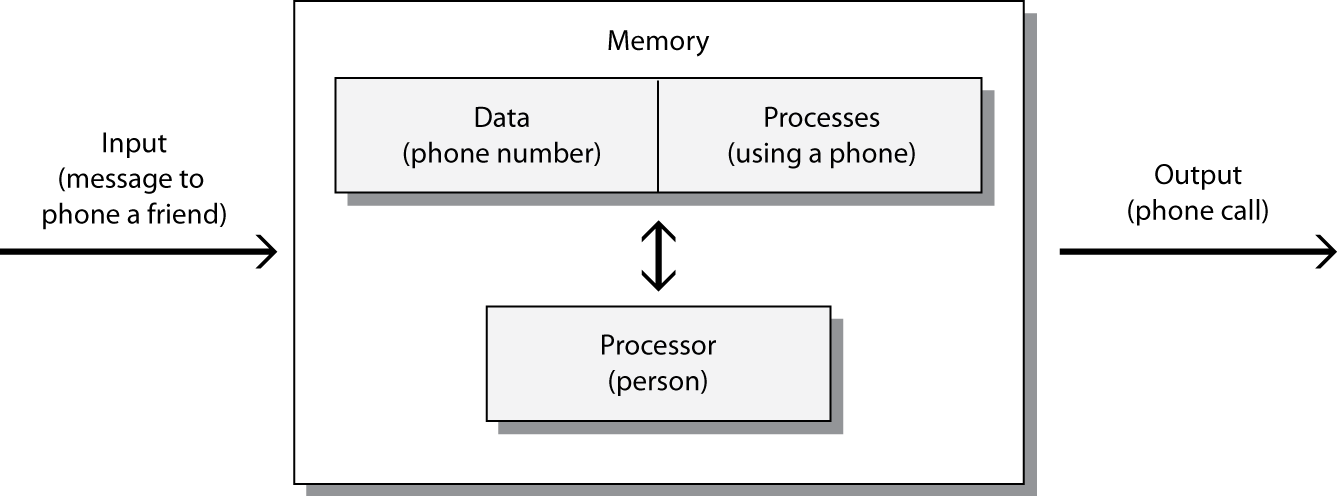
\includegraphics{Figures/Section 1/Simon-Newell.png}

To understand this model, consider a person arriving on a flight who has
agreed to meet a fellow traveler in the terminal. She receives a text
message to meet her friend at B27. The message is input to her human
information processing system. She retrieves the process for
interpreting the message (i.e., decoding that B27 means terminal B and
gate 27) and finds the terminal and gate. The person then walks to the
terminal and gate, the output. Sometimes these processes are so well
ingrained in our memory that we never think about retrieving them. We
just do them automatically.

Human information processing systems are easily overloaded. Our memory
is limited, and our ability to process data is restricted; thus we use a
variety of external tools to extend and augment our capacities. A
contacts app is an instance of external data memory. A recipe, a
description of the process for preparing food, is an example of external
process memory. Smartphones are now the external processor of choice
that we use to augment our limited processing capacity.

The original model of human information processing can be extended to
include external memory, for storing data and processes, and external
processors, for executing processes.

\textbf{\emph{Missing this image}}

This model of augmented human information processing translates directly
to an organizational setting. Organizations collect inputs from the
environment: market research, customer complaints, and competitor
actions. They process these data and produce outputs: sales campaigns,
new products, price changes, and so on. The following figure gives an
example of how an organization might process data. As a result of some
market research (input), a marketing analyst (an internal processor)
retrieves sales data (data) and does a sales forecast (process). The
analyst also requests a marketing consultant (an external processor) to
analyze (process) some demographic reports (data) before deciding to
launch a new sales campaign (output).

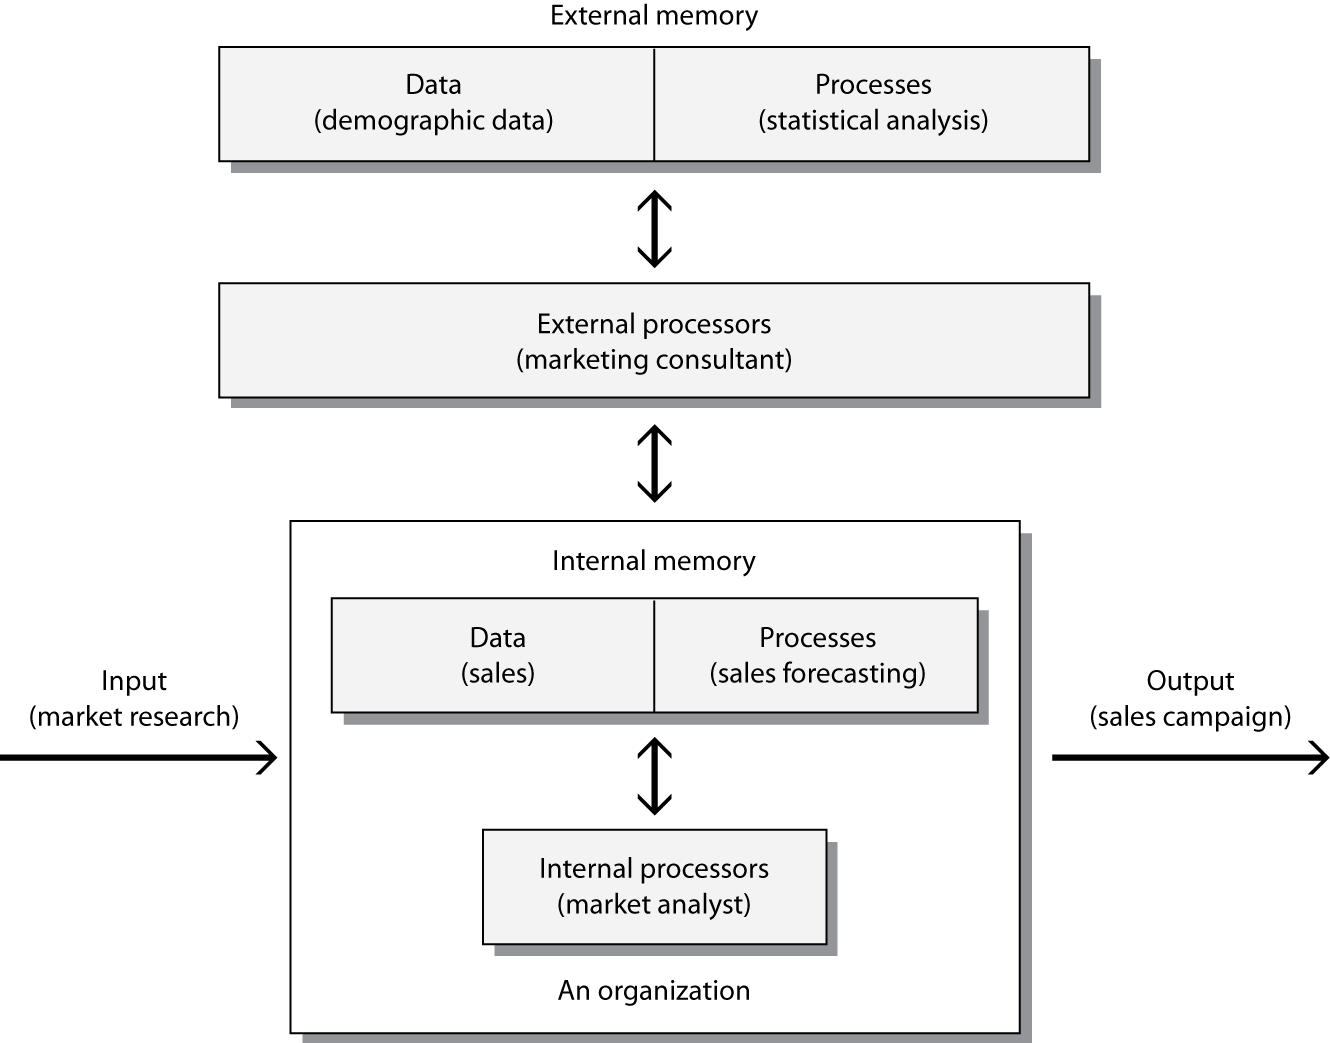
\includegraphics{Figures/Section 1/org info processing.png}

An organization's memory comes in a variety of forms, as you will see in
Chapter 1. This memory also can be divided into data and processes. The
data part may contain information about customers. The process portion
may store details of how to handle a customer order. Organizations use a
variety of processors to handle data, including people and computers.
Organizations also rely on external sources to extend their information
processing capacity. For example, a business may use a specialist credit
agency to check a customer's creditworthiness, or an engineering firm
may use a cloud computing service for structural analysis of a bridge.
Viewed this way, the augmented human information processing model
becomes a pattern for an organizational information processing system.

This book focuses on the data side of organizational memory. While it is
primarily concerned with data stored within the organization, there is
also coverage of data in external memory. The process side of
organizational memory is typically covered in a systems analysis and
design or a business process management course.

\newpage

\hypertarget{managing-data}{%
\section{Managing Data}\label{managing-data}}

\begin{quote}
\emph{All the value of this company is in its people. If you burned down
all our plants, and we just kept our people and our information files,
we should soon be as strong as ever.}

Thomas Watson, Jr., former chairman of IBM\footnote{Quinn, J. B. (1994). Appraising intellectual assets. *The
  McKinsey Quarterly*(2), 90-96.}
\end{quote}

\hypertarget{learning-objectives}{%
\subsection*{Learning objectives}\label{learning-objectives}}
\addcontentsline{toc}{subsection}{Learning objectives}

Students completing this chapter will

\begin{itemize}
\item
  understand the key concepts of data management;
\item
  recognize that there are many components of an organization's
  memory;
\item
  understand the problems with existing data management systems;
\item
  realize that successful data management requires an integrated
  understanding of organizational behavior and information technology.
\end{itemize}

\hypertarget{introduction}{%
\subsection*{Introduction}\label{introduction}}
\addcontentsline{toc}{subsection}{Introduction}

Imagine what would happen to a bank that forgot who owed it money or a
magazine that lost the names and addresses of its subscribers. Both
would soon be in serious difficulty, if not out of business.
Organizations have data management systems to record the myriad of
details necessary for transacting business and making informed
decisions. Since the birth of agriculture, societies and organizations
have recorded data. The system may be as simple as carving a notch in a
stick to keep a tally, or as intricate as modern database technology. A
memory system can be as personal as a to-do list or as public as a
library.

The management of organizational data, generally known as data
management, requires skills in designing, using, and managing the memory
systems of modern organizations. It requires multiple perspectives. Data
managers need to see the organization as a social system and to
understand data management technology. The integration of these views,
the socio-technical perspective, is a prerequisite for successful data
management.

Individuals also need to manage data. You undoubtedly are more familiar
with individual memory management systems. They provide a convenient way
of introducing some of the key concepts of data management.

\hypertarget{individual-data-management}{%
\subsection*{Individual data management}\label{individual-data-management}}
\addcontentsline{toc}{subsection}{Individual data management}

As humans, we are well aware of our limited capacity to remember many
things. The brain, our internal memory, can get overloaded with too much
detail, and its memory decays with time. We store a few things
internally: our cell phone number, where we last parked our car, and
faces of people we have met recently. We use external memory to keep
track of those many things we would like to remember. External memory
comes in a variety of forms.

On our smartphones, we have calendars to remind us of meetings and
project deadlines. We have a contact app to record the addresses and
phone numbers of those we contact frequently. We use to-do lists to
remind us of the things we must do today or this week. The interesting
thing about these aides-mémoire is that each has a unique way of storing
data and supporting its rapid retrieval.

Calendars come in many shapes and forms, but they are all based on the
same organizing principle. A set amount of space is allocated for each
day of the year, and the spaces are organized in date and time order,
which supports rapid retrieval. Some calendars have added features to
speed up access. For example, electronic calendars usually have a button
to select today's data.

\emph{A calendar}

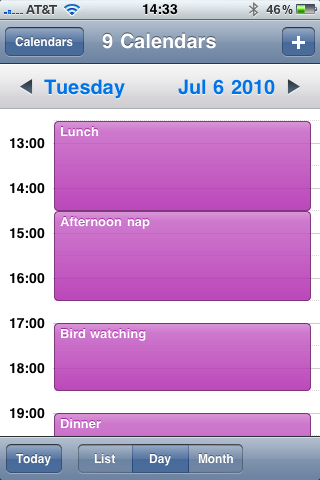
\includegraphics{Figures/Chapter 1/calendar.png}

Address books also have a standard format. They typically contain
predefined spaces for storing address details (e.g., name, company,
phone, and email). Access is often supported by a set of buttons for
each letter of the alphabet and a search engine.

\emph{An address book}

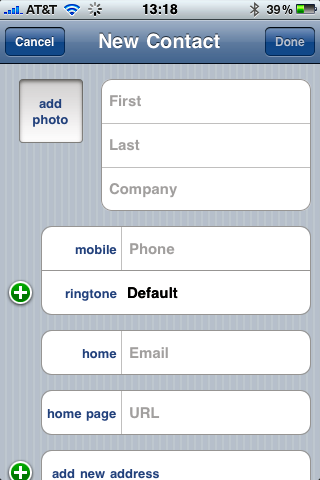
\includegraphics{Figures/Chapter 1/address book.png}

The structure of to-do lists tends to be fairly standard. They are often
set up in list format with a small left-hand margin. The idea is to
enter each item to be done on the right side of the screen. The left
side is used to check or mark those tasks that have been completed. The
beauty of the check method is that you can quickly scan the left side to
identify incomplete tasks.

\emph{A to-do or reminder list}

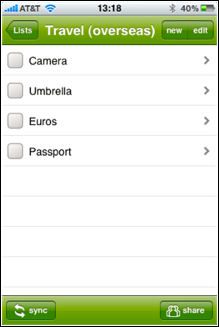
\includegraphics[width=3.33333in,height=\textheight]{Figures/Chapter 1/todo list new.png}

Many people use some form of the individual memory systems just
described. They are typically included in the suite of standard
applications for a smart phone.

These three examples of individual memory systems illustrate some
features common to all data management systems:

\begin{itemize}
\item
  There is a storage medium. Data are stored electronically in each
  case.
\item
  There is a structure for storing data. For instance, the address
  book has labeled spaces for entering pertinent data.
\item
  The interface organized for rapid data entry and retrieval. A
  calendar is stored in date and time sequence so that the data space
  for any appointment for a particular day can be found quickly.
\item
  The selection of a data management system frequently requires a
  trade-off decision. In these examples, the trade-off is screen
  dimensions versus the amount of data that can be seen without
  scrolling. For example, you will notice the address book screen is
  truncated and will need to be scrolled to see full address details.
\end{itemize}

\begin{quote}
❓\emph{Skill builder}

Smart phones have dramatically changed individual data management. We
now have calendars, address books, to-do lists, and many more apps
literally in our hands. What individual data are still difficult to
manage? What might be the characteristics of an app for these data?
\end{quote}

There are differences between internal and external memories. Our
internal memory is small, fast, and convenient (our brain is always with
us---well, most of the time). External memory is often slower to
reference and not always as convenient. The two systems are
interconnected. We rely on our internal memory to access external
memory. Our internal memory and our brain's processing skills manage the
use of external memories. For example, we depend on our internal memory
to recall how to use our smartphone and its apps. Again, we see some
trade-offs. Ideally, we would like to store everything in our fast and
convenient internal memory, but its limited capacity means that we are
forced to use external memory for many items.

\hypertarget{organizational-data-management}{%
\subsection*{Organizational data management}\label{organizational-data-management}}
\addcontentsline{toc}{subsection}{Organizational data management}

Organizations, like people, need to remember many things. If you look
around any office, you will see examples of the apparatus of
organizational memory: people, bookshelves, planning boards, and
computers. The same principles found in individual memory systems apply
to an organization's data management systems.

There is a storage medium. In the case of computers, the storage medium
varies. Small files might be stored on a USB drive and large, archival
files on a magnetic disk. The chapter \emph{Data Structure and Storage}
discusses electronic storage media in more detail.

A table is a common structure for storing data. For example, if we want
to store details of customers, we can set up a table with each row
containing individual details of a customer and each column containing
data on a particular feature (e.g., customer code).

Storage devices are organized for rapid data entry and retrieval. Time
is the manager's enemy: too many things to be done in too little time.
Customers expect rapid responses to their questions and quick processing
of their transactions. Rapid data access is a key goal of nearly all
data management systems, but it always comes at a price. Fast access
memories cost more, so there is nearly always a trade-off between access
speed and cost.

As you will see, selecting \emph{how} and \emph{where} to store organizational
data frequently involves a trade-off. Data managers need to know and
understand what the compromises entail. They must know the key questions
to ask when evaluating choices.

When we move from individual to organizational memory, some other
factors come into play. To understand these factors, we need to review
the different types of information systems. The automation of routine
business transactions was the earliest application of information
technology to business. A transaction processing system (TPS) handles
common business tasks such as accounting, inventory, purchasing, and
sales. The realization that the data collected by these systems could be
sorted, summarized, and rearranged gave birth to the notion of a
management information system (MIS). Furthermore, it was recognized that
when internal data captured by a TPS is combined with appropriate
external data, the raw material is available for a decision support
system (DSS). Online analytical processing (OLAP), data mining, business
intelligence (BI), and machine learning are techniques analyzing data
captured by business transactions and gathered from other sources (these
systems are covered in detail in Chapter 14). The purpose of each of
these systems is described in the following table and their
interrelationship can be understood by examining the information systems
cycle.

\emph{Types of information systems}

\begin{longtable}[]{@{}
  >{\raggedright\arraybackslash}p{(\columnwidth - 4\tabcolsep) * \real{0.04}}
  >{\raggedright\arraybackslash}p{(\columnwidth - 4\tabcolsep) * \real{0.22}}
  >{\raggedright\arraybackslash}p{(\columnwidth - 4\tabcolsep) * \real{0.74}}@{}}
\toprule
& Type of in formation system & System's purpose \\
\midrule
\endhead
TPS & Tr ansaction p rocessing system & Collect and store data from routine transactions \\
MIS & M anagement in formation system & Convert data from a TPS into information for planning, controlling, and managing an organization \\
DSS & Decision support system & Support managerial decision making by providing models for processing and analyzing data \\
BI & Business int elligence & Gather, store, and analyze data to improve decision making \\
OLAP & Online a nalytical p rocessing & Provide a multidimensional view of data \\
& Data mining & Use of statistical analysis and artificial intelligence techniques to identify hidden relationships in data \\
& Machine learning & Using software to make decisions or recommendations traditionally made by humans. \\
\bottomrule
\end{longtable}

\hypertarget{the-information-systems-cycle}{%
\subsubsection*{The information systems cycle}\label{the-information-systems-cycle}}
\addcontentsline{toc}{subsubsection}{The information systems cycle}

The various systems and technologies found in an organization are linked
in a cycle. The routine ongoing business of the organization is
processed by TPSs, the systems that handle the present. Data collected
by TPSs are stored in databases, a record of the past, the history of
the organization and its interaction with those with whom it conducts
business. These data are converted into information by analysts using a
variety of software (e.g., a DSS). These technologies are used by the
organization to prepare for the future (e.g., sales in Finland have
expanded, so we will build a new service center in Helsinki). The
business systems created to prepare for the future determine the
transactions the company will process and the data that will be
collected, and the process continues. The entire cycle is driven by
people using technology (e.g., a customer booking a hotel room via a Web
browser).

\emph{The information systems cycle}

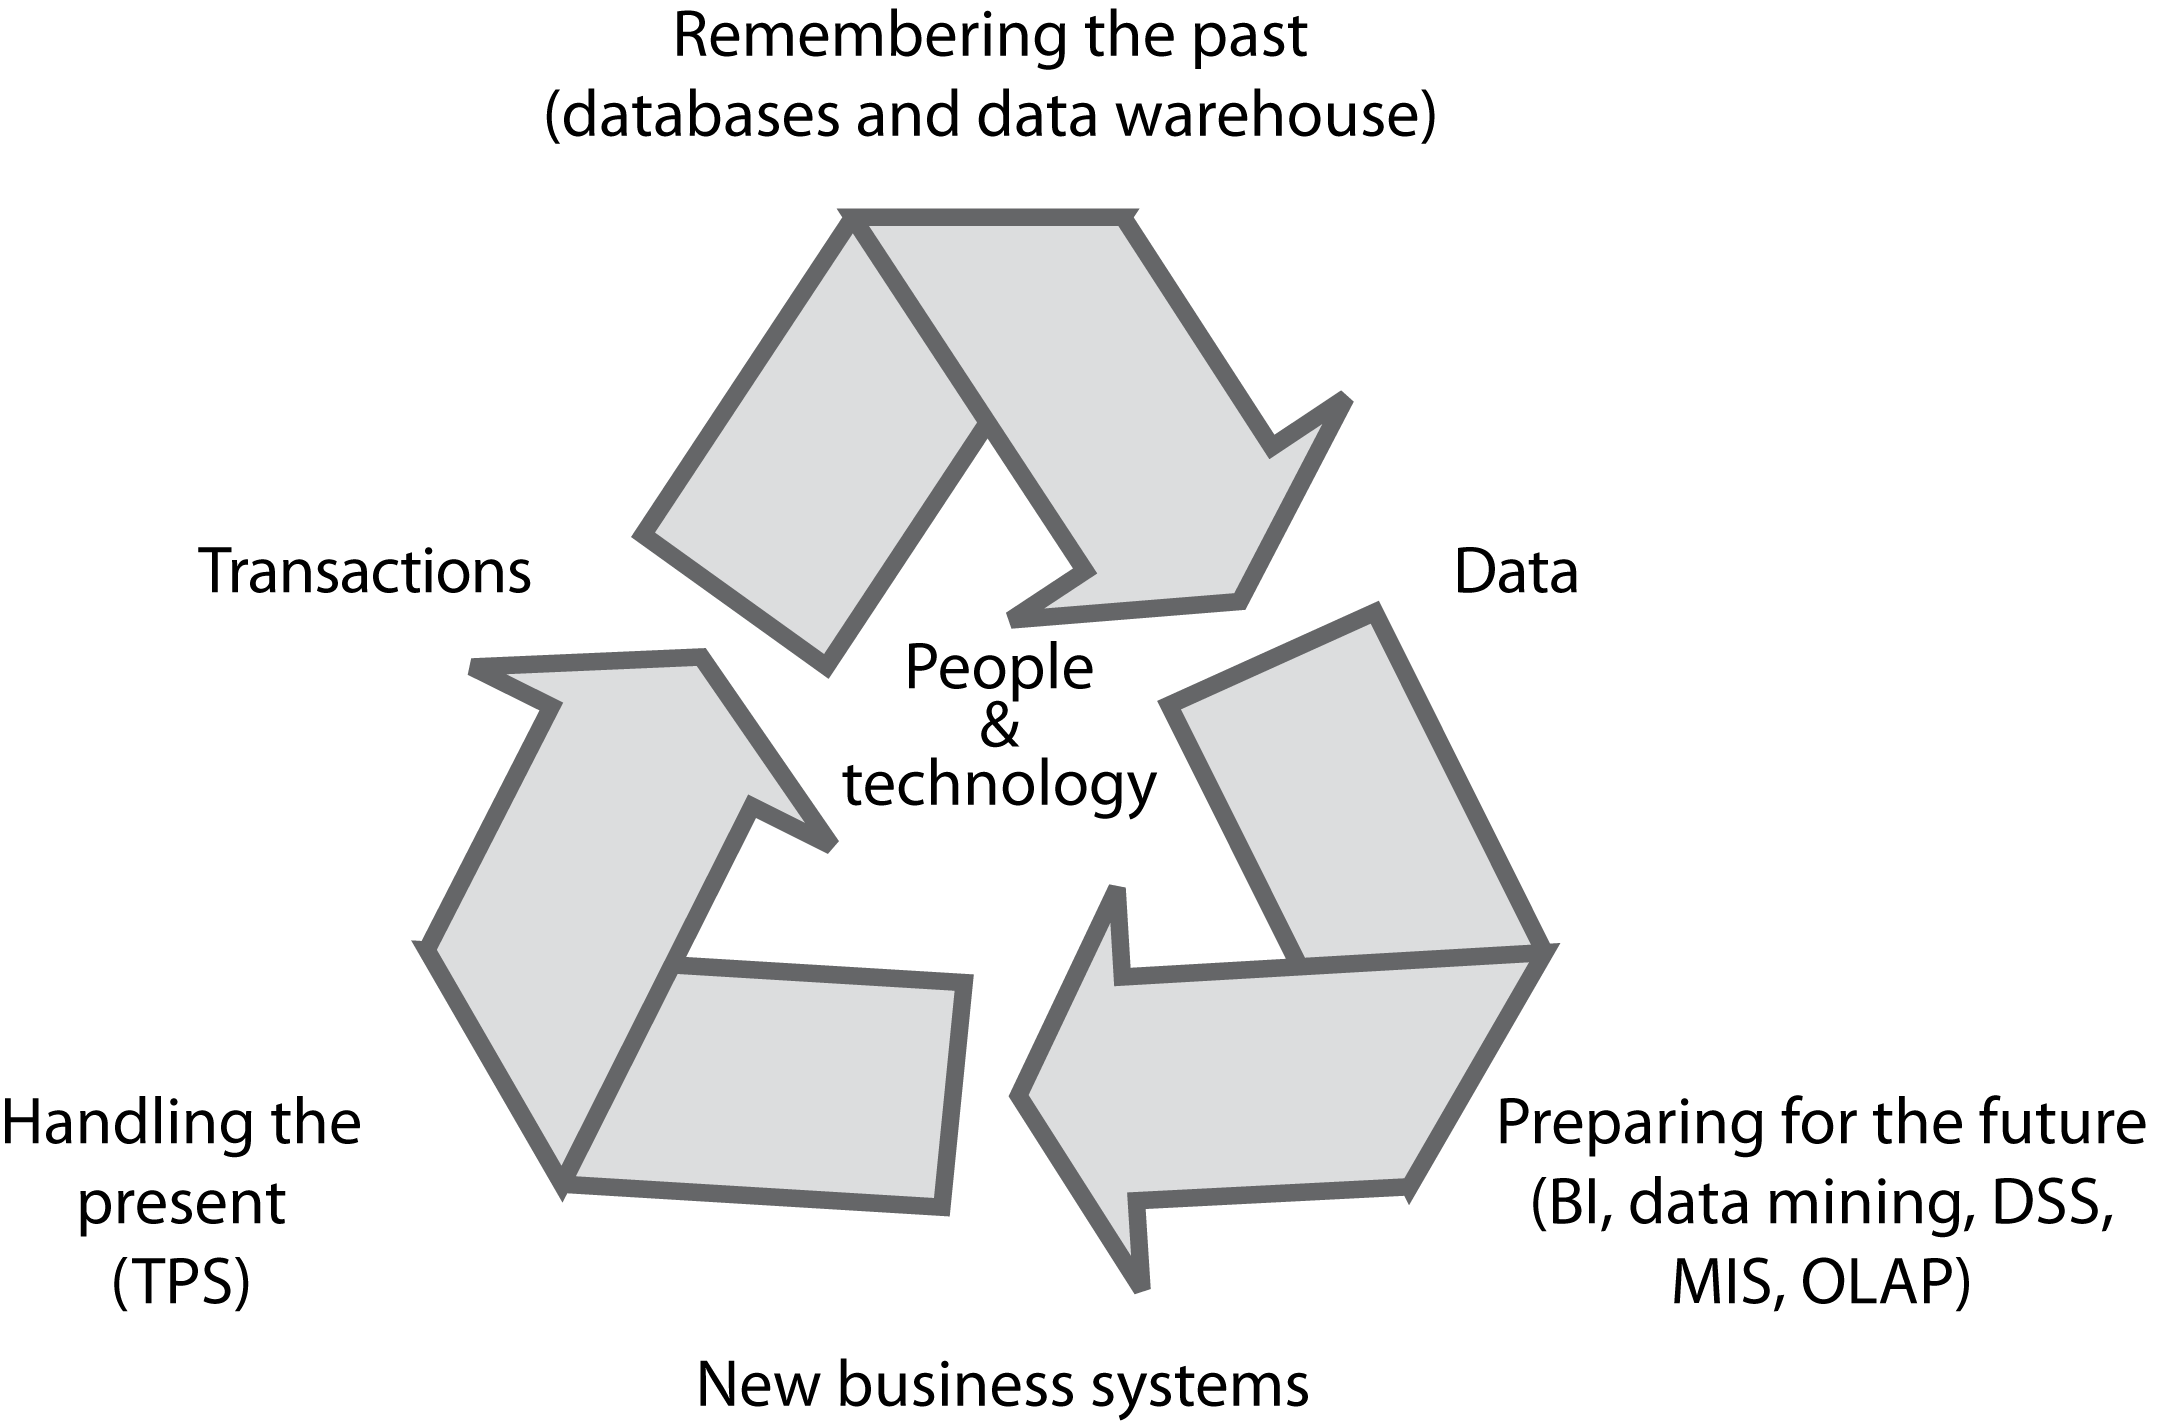
\includegraphics{Figures/Chapter 1/IS cycle.png}

Decision making, or preparing for the future, is the central activity of
modern organizations. Today's organizations are busy turning out goods,
services, and decisions. Knowledge and information workers, over half of
the U.S. labor force, produce the bulk of GDP. Many of these people are
decision makers. Their success, and their organization's as well,
depends on the quality of their decisions.

Industrial society is a producer of goods, and the hallmark of success
is product quality. Japanese manufacturers convincingly demonstrated
that focusing on product quality is the key to market leadership and
profitability. The methods and the philosophy of quality gurus, such as
W. Edwards Deming, have been internationally recognized and adopted by
many providers of goods and services. We are now in the information age
as is evidenced by the key consumer products of the times, such as smart
phones, tablets, and wearables. These are all information appliances,
and they are supported by a host of information services. For example,
consider how Apple connects together its various devices and services
through cloud-based systems. For example, a person can buy an electronic
book from Apple's store to read with the iBooks app on an iPhone or
iPad.

In the information society, which is based on innovation, knowledge, and
services, the key determinant of success has shifted from product
quality to decision quality. In the turbulent environment of global
business, successful organizations are those able to quickly make
high-quality decisions about what customers will buy, how much they will
pay, and how to deliver a high-quality experience with a minimum of
fuss. Companies are very dependent on information systems to create
value for their customers.

\hypertarget{desirable-attributes-of-data}{%
\subsubsection*{Desirable attributes of data}\label{desirable-attributes-of-data}}
\addcontentsline{toc}{subsubsection}{Desirable attributes of data}

Once we realize the critical importance of data to organizations, we can
recognize some desirable attributes of data.

\emph{Desirable attributes of data}

\begin{longtable}[]{@{}ll@{}}
\toprule
Shareable & Readily accessed by more than one person at a time \\
\midrule
\endhead
Transportable & Easily moved to a decision maker \\
Secure & Protected from destruction and unauthorized use \\
Accurate & Reliable, precise records \\
Timely & Current and up-to-date \\
Relevant & Appropriate to the decision \\
\bottomrule
\end{longtable}

\hypertarget{shareable}{%
\paragraph*{Shareable}\label{shareable}}
\addcontentsline{toc}{paragraph}{Shareable}

Organizations contain many decision makers. There are occasions when
more than one person will require access to the same data at the same
time. For example, in a large bank it would not be uncommon for two
customer representatives simultaneously to want data on the latest rate
for a three-year certificate of deposit. As data become more volatile,
shareability becomes more of a problem. Consider a restaurant. The
permanent menu is printed, today's special might be displayed on a
blackboard, and the waiter tells you what is no longer available.

\hypertarget{transportable}{%
\paragraph*{Transportable}\label{transportable}}
\addcontentsline{toc}{paragraph}{Transportable}

Data should be transportable from their storage location to the decision
maker. Technologies that transport data have a long history. Homing
pigeons were used to relay messages by the Egyptians and Persians 3,000
years ago. The telephone revolutionized business and social life because
it rapidly transmitted voice data. Computers have changed the nature of
many aspects of business because they enable the transport of text,
visuals, voice and video.

Today, transportability is more than just getting data to a decision
maker's desk. It means getting product availability data to a
salesperson in a client's office or advising a delivery driver, en
route, of address details for an urgent parcel pickup. The general
notion is that decision makers should have access to relevant data
whenever and wherever required, although many organizations are still
some way from reaching this target.

\hypertarget{secure}{%
\paragraph*{Secure}\label{secure}}
\addcontentsline{toc}{paragraph}{Secure}

In an information society, organizations value data as a resource. As
you have already learned, data support day-to-day business transactions
and decision making. Because the forgetful organization will soon be out
of business, organizations are very vigilant in protecting their data.
There are a number of actions that organizations take to protect data
against loss, sabotage, and theft. A common approach is to duplicate
data and store the copy, or copies, at other locations. This technique
is popular for data stored in computer systems. Access to data is often
restricted through the use of physical barriers (e.g., a vault) or
electronic barriers (e.g., a password). Another approach, which is
popular with firms that employ knowledge workers, is a noncompete
contract. For example, some software companies legally restrain computer
programmers from working for a competitor for two years after they
leave, hoping to prevent the transfer of valuable data, in the form of
the programmer's knowledge of software, to competitors.

\hypertarget{accurate}{%
\paragraph*{Accurate}\label{accurate}}
\addcontentsline{toc}{paragraph}{Accurate}

You probably recall friends who excel in exams because of their good
memories. Similarly, organizations with an accurate memory will do
better than their less precise competitors. Organizations need to
remember many details precisely. For example, an airline needs accurate
data to predict the demand for each of its flights. The quality of
decision making will drop dramatically if managers use a data management
system riddled with errors.

Polluted data threatens a firm's profitability. One study suggests that
missing, wrong, and otherwise bad data cost U.S. firms billions of
dollars annually. The consequences of bad data include improper billing,
cost overruns, delivery delays, and product recalls. Because data
accuracy is so critical, organizations need to be watchful when
capturing data---the point at which data accuracy is most vulnerable.

\hypertarget{timely}{%
\paragraph*{Timely}\label{timely}}
\addcontentsline{toc}{paragraph}{Timely}

The value of a collection of data is often determined by its age. You
can fantasize about how rich you would be if you knew tomorrow's stock
prices. Although decision makers are most interested in current data,
the required currency of data can vary with the task. Operational
managers often want real-time data. They want to tap the pulse of the
production line so that they can react quickly to machine breakdowns or
quality slippages. In contrast, strategic planners might be content with
data that are months old because they are more concerned with detecting
long-term trends.

\hypertarget{relevant}{%
\paragraph*{Relevant}\label{relevant}}
\addcontentsline{toc}{paragraph}{Relevant}

Organizations must maintain data that are relevant to transaction
processing and decision making. In processing a credit card application,
the most relevant data might be the customer's credit history, current
employment status, and income level. Hair color would be irrelevant.
When assessing the success of a new product line, a marketing manager
probably wants an aggregate report of sales by marketing region. A
voluminous report detailing every sale would be irrelevant. Data are
relevant when they pertain directly to the decision and are aggregated
appropriately.

Relevance is a key concern in designing a data management system.
Clients have to decide what should be stored because it is pertinent now
or could have future relevance. Of course, identifying data that might
be relevant in the future is difficult, and there is a tendency to
accumulate too much. Relevance is also an important consideration when
extracting and processing data from a data management system. Provided
the germane data are available, query languages can be used to aggregate
data appropriately.

In the final years of the twentieth century, organizations started to
share much of their data, both high and low volatility, via the Web.
This move increased shareability, timeliness, and availability, and it
has lowered the cost of distributing data.

In summary, a data management system for maintaining an organization's
memory supports transaction processing, remembering the past, and
decision making. Its contents must be shareable, secure, and accurate.
Ideally, the clients of a data management system must be able to get
timely and relevant data when and where required. A major challenge for
data management professionals is to create data management systems that
meet these criteria. Unfortunately, many existing systems fail in this
regard, though we can understand some of the reasons why by reviewing
the components of existing organizational memory systems.

\hypertarget{components-of-organizational-memory}{%
\subsubsection*{Components of organizational memory}\label{components-of-organizational-memory}}
\addcontentsline{toc}{subsubsection}{Components of organizational memory}

An organization's memory resides on a variety of media in a variety of
ways. It is in people, standard operating procedures, roles,
organizational culture, physical storage equipment, and electronic
devices. It is scattered around the organization like pieces of a jigsaw
puzzle designed by a berserk artist. The pieces don't fit together, they
sometimes overlap, there are gaps, and there are no edge pieces to
define the boundaries. Organizations struggle to design structures and
use data management technology to link some of the pieces. To understand
the complexity of this wicked puzzle, we need to examine some of the
pieces. Data managers have a particular need to understand the different
forms of organizational memory because their activities often influence
a number of the components.

\emph{Components of organizational memory}

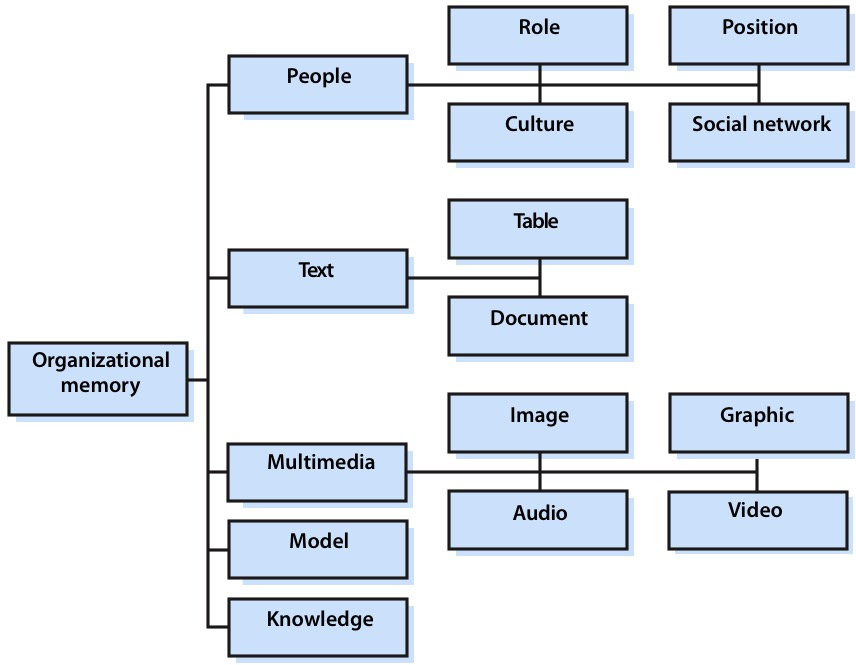
\includegraphics{Figures/Chapter 1/org memory components.jpg}

\hypertarget{people}{%
\paragraph*{People}\label{people}}
\addcontentsline{toc}{paragraph}{People}

People are the linchpin of an organization's memory. They recall prior
decisions and business actions. They create, maintain, evolve, and use
data management systems. They are the major component of an
organization's memory because they know how to use many of the other
components. People extract data from the various elements of
organizational memory to provide as complete a picture of a situation as
possible.

Each person in an organization has a role and a position in the
hierarchy. Role and position are both devices for remembering how the
organization functions and how to process data. By labeling people
(e.g., Chief Information Officer) and placing their names on an
organizational chart, the organization creates another form of
organizational memory.

Organizational culture is the shared beliefs, values, attitudes, and
norms that influence the behavior and expectations of each person in an
organization. As a long-lived and stable memory system, culture
determines acceptable behavior and influences decision making.

People develop skills for doing their particular job---learning what to
do, how to do it, and who can help them get things done. For example,
they might discover someone in employee benefits who can handle
personnel problems or a contact in a software company who can answer
questions promptly. These social networks, which often take years to
develop, are used to make things happen and to learn about the business
environment. Despite their high value, they are rarely documented, at
least not beyond an address book, and they are typically lost when a
person leaves an organization.

\textbf{Conversations} are an important method for knowledge workers to
create, modify, and share organizational memory and to build
relationships and social networks. Discussions with customers are a key
device for learning how to improve an organization's products and
services and learning about competitors. The \textbf{\emph{conversational
company}} can detect change faster and react more rapidly. The
telephone, instant message, e-mail, coffee machine, cocktail hour, and
cafeteria are all devices for promoting conversation and creating
networks. Some firms deliberately create structures for supporting
dialog to make the people component of organizational memory more
effective.

Standard operating procedures exist for many organizational tasks.
Processing a credit application, selecting a marketing trainee, and
preparing a departmental budget are typical procedures that are clearly
defined by many organizations. They are described on Web pages, computer
programs, and job specifications. They are the way an organization
remembers how to perform routine activities.

Successful people learn how to use organizational memory. They learn
what data are stored where, how to retrieve them, and how to put them
together. In promoting a new product, a salesperson might send the
prospect a package containing some brochures and an email of a product
review in a trade journal, and supply the phone number and e-mail
address of the firm's technical expert for that product. People's recall
of how to use organizational memory is the core component of
organizational memory. Academics call this \textbf{metamemory}; people in
business call it \emph{\textbf{l}earning the ropes}. New employees spend a great
deal of time building their metamemory so that they can use
organizational memory effectively. Without this knowledge,
organizational memory has little value.

\hypertarget{tables}{%
\paragraph*{Tables}\label{tables}}
\addcontentsline{toc}{paragraph}{Tables}

A table is a common form of storing organizational data. The following
table shows a price list in tabular form. Often, the first row defines
the meaning of data in subsequent rows.

\emph{A price list}

\begin{longtable}[]{@{}ll@{}}
\toprule
Product & Price \\
\midrule
\endhead
Pocket knife--Nile & 4.5 \\
Compass & 10 \\
Geopositioning system & 500 \\
Map measure & 4.9 \\
\bottomrule
\end{longtable}

A table is a general form that describes a variety of other structures
used to store data. Computer-based files are tables or can be
transformed into tables; the same is true for general ledgers,
worksheets, and spreadsheets. Accounting systems make frequent use of
tables. As you will discover in the next section, the table is the
central structure of the relational database model.

Data stored in tables typically have certain characteristics:

\begin{itemize}
\item
  Data in one column are of the same type. For example, each cell of
  the column headed ``Price'' contains a number. (Of course, the
  exception is the first row of each column, which contains the title
  of the column.)
\item
  Data are limited by the width of the available space.
\end{itemize}

Rapid searching is one of the prime advantages of a table. For example,
if the price list is sorted by product name, you can quickly find the
price of any product.

Tables are a common form of storing organizational data because their
structure is readily understood. People learn to read and build tables
in the early years of their schooling. Also, a great deal of the data
that organizations want to remember can be stored in tabular form.

\hypertarget{documents}{%
\paragraph*{Documents}\label{documents}}
\addcontentsline{toc}{paragraph}{Documents}

A \textbf{document}---of which reports, manuals, brochures, and memos are
examples---is a common medium for storing organizational data. Although
documents may be subdivided into chapters, sections, paragraphs, and
sentences, they lack the regularity and discipline of a table. Each row
of a table has the same number of columns, but each paragraph of a
document does not have the same number of sentences.

Most documents are now stored electronically. Because of the widespread
use of word processing, text files are a common means of storing
documents. Typically, such files are read sequentially like a book.
Although there is support for limited searching of the text, such as
finding the next occurrence of a specified text string, text files are
usually processed linearly.

Hypertext, the familiar linking technology of the Web, supports
nonlinear document processing. A hypertext document has built-in
linkages between sections of text that permit the reader to jump quickly
from one part to another. As a result, readers can find data they
require more rapidly.

Although hypertext is certainly more reader-friendly than a flat,
sequential text file, it takes time and expertise to establish the links
between the various parts of the text and to other documents. Someone
familiar with the topic has to decide what should be linked and then
establish these links. While it takes the author more time to prepare a
document this way, the payoff is the speed at which readers of the
document can find what they want.

\hypertarget{multimedia}{%
\paragraph*{Multimedia}\label{multimedia}}
\addcontentsline{toc}{paragraph}{Multimedia}

Many Web sites display multimedia objects, such as sound and video
clips. Automotive company Web sites have video clips of cars, music
outlets provide sound clips of new releases, and clothing companies have
online catalogs displaying photos of their latest products. Maintaining
a Web site, because of the many multimedia objects that some sites
contain, has become a significant data management problem for some
organizations. Consider the different types of data that a news outfit
such as the British Broadcasting Corporation (BBC) has to store to
provide a timely, informative, and engaging Web site.

\hypertarget{images}{%
\paragraph*{Images}\label{images}}
\addcontentsline{toc}{paragraph}{Images}

Images are visual data: photographs and sketches. Image banks are
maintained for several reasons. \emph{First\textbf{,}} images are widely used for
identification and security. Police departments keep fingerprints and
mug shots. \emph{Second}, images are used as evidence. Highly valuable items
such as paintings and jewelry often are photographed for insurance
records. \emph{Third}, images are used for advertising and promotional
campaigns, and organizations need to maintain records of material used
in these ventures. Image archiving and retrieval are essential for
mail-order companies, which often produce several photo-laden catalogs
every year. \emph{Fourth}, some organizations specialize in selling images
and maintain extensive libraries of clip art and photographs.

\hypertarget{graphics}{%
\paragraph*{Graphics}\label{graphics}}
\addcontentsline{toc}{paragraph}{Graphics}

Maps and engineering drawings are examples of electronically stored
graphics. An organization might maintain a map of sales territories and
customers. Manufacturers have extensive libraries of engineering
drawings that define the products they produce. Graphics often contain a
high level of detail. An engineering drawing will define the dimensions
of all parts and may refer to other drawings for finer detail about any
components.

A graphic differs from an image in that it contains explicitly embedded
data. Consider the difference between an engineering plan for a widget
and a photograph of the same item. An engineering plan shows dimensional
data and may describe the composition of the various components. The
embedded data are used to manufacture the widget. A photograph of a
widget does not have embedded data and contains insufficient data to
manufacture the product. An industrial spy will receive far more for an
engineering plan than for a photograph of a widget.

A geographic information systems \textbf{(}GIS\textbf{)} is a specialized
graphical storage system for geographic data. The underlying structure
of a GIS is a map on which data are displayed. A power company can use a
GIS to store and display data about its electricity grid and the
location of transformers. Using a pointing device such as a mouse, an
engineer can click on a transformer's location to display a window of
data about the transformer (e.g., type, capacity, installation date, and
repair history). GISs have found widespread use in governments and
organizations that have geographically dispersed resources.

\hypertarget{audio}{%
\paragraph*{Audio}\label{audio}}
\addcontentsline{toc}{paragraph}{Audio}

News organizations, such as National Public Radio (NPR), provide audio
versions of their new stories for replay. Some firms conduct a great
deal of their business by phone. In many cases, it is important to
maintain a record of the conversation between the customer and the
firm's representative. The Royal Hong Kong Jockey Club, which covers
horse racing gambling in Hong Kong, records all conversations between
its operators and customers. Phone calls are stored on a highly
specialized voice recorder, which records the time of the call and other
data necessary for rapid retrieval. In the case of a customer dispute,
an operator can play back the original conversation.

\hypertarget{video}{%
\paragraph*{Video}\label{video}}
\addcontentsline{toc}{paragraph}{Video}

A video clip can give a potential customer additional detail that cannot
be readily conveyed by text or a still image. Consequently, some auto
companies use video and virtual reality to promote their cars. On a
visit to Toyota's Web site, you can view video clips of the latest
models or rotate an image to view a car from multiple angles.

\hypertarget{models}{%
\paragraph*{Models}\label{models}}
\addcontentsline{toc}{paragraph}{Models}

Organizations build mathematical models to describe their business.
These models, usually placed in the broader category of DSS, are then
used to analyze existing problems and forecast future business
conditions. A mathematical model can often produce substantial benefits
to the organization.

\hypertarget{knowledge}{%
\paragraph*{Knowledge}\label{knowledge}}
\addcontentsline{toc}{paragraph}{Knowledge}

Organizations build systems to capture the knowledge of their
experienced decision makers and problem solvers. This expertise is
typically represented as a set of rules, semantic nets, and frames in a
knowledge base, another form of organizational memory.

\hypertarget{decisions}{%
\paragraph*{Decisions}\label{decisions}}
\addcontentsline{toc}{paragraph}{Decisions}

Decision making is the central activity of modern organizations. Very
few organizations, however, have a formal system for recording
decisions. Most keep the minutes of meetings, but these are often very
brief and record only a meeting's outcome. Because they do not record
details such as the objectives, criteria, assumptions, and alternatives
that were considered prior to making a decision, there is no formal
audit trail for decision making. As a result, most organizations rely on
humans to remember the circumstances and details of prior decisions.

\hypertarget{specialized-memories}{%
\paragraph*{Specialized memories}\label{specialized-memories}}
\addcontentsline{toc}{paragraph}{Specialized memories}

Because of the particular nature of their business, some organizations
maintain memories rarely found elsewhere. Perfume companies, for
instance, maintain a library of scents, and paint manufacturers and dye
makers catalog colors.

\hypertarget{components-of-organizational-memory-1}{%
\subsubsection*{Components of organizational memory}\label{components-of-organizational-memory-1}}
\addcontentsline{toc}{subsubsection}{Components of organizational memory}

Organizations are not limited to their own memory stores. There are
firms whose business is to store data for resale to other organizations.
Such businesses have existed for many years and are growing as the
importance of data in a postindustrial society expands. U.S. lawyers can
use document management services to access the laws and court decisions
of all 50 American states and the U.S. federal government. Similar legal
data services exist in many other nations. There is a range of other
services that provide news, financial, business, scientific, and medical
data.

\hypertarget{problems-with-data-management-systems}{%
\subsection*{Problems with data management systems}\label{problems-with-data-management-systems}}
\addcontentsline{toc}{subsection}{Problems with data management systems}

Successful management of data is a critical skill for nearly every
organization. Yet few have gained complete mastery, and there are a
variety of problems that typically afflict data management in most
firms.

\emph{Problems with organizational data management systems}

\begin{longtable}[]{@{}
  >{\raggedright\arraybackslash}p{(\columnwidth - 2\tabcolsep) * \real{0.26}}
  >{\raggedright\arraybackslash}p{(\columnwidth - 2\tabcolsep) * \real{0.74}}@{}}
\toprule
Redundancy & Same data are stored in different systems \\
\midrule
\endhead
Lack of data control & Data are poorly managed \\
Poor interface & Data are difficult to access \\
Delays & There are frequently delays following requests for reports \\
Lack of reality & Data management systems do not reflect the complexity of the real world \\
Lack of data integration & Data are dispersed across different systems \\
\bottomrule
\end{longtable}

\hypertarget{redundancy}{%
\subsubsection*{Redundancy}\label{redundancy}}
\addcontentsline{toc}{subsubsection}{Redundancy}

In many cases, data management systems have grown haphazardly. As a
result, it is often the situation that the same data are stored in
several different memories. The classic example is a customer's address,
which might be stored in the sales reporting system, accounts receivable
system, and the salesperson's address book. The danger is that when the
customer changes address, the alteration is not recorded in all systems.
Data redundancy causes additional work because the same item must be
entered several times. Redundancy causes confusion when what is
supposedly the same item has different values.

\hypertarget{lack-of-data-control}{%
\subsubsection*{Lack of data control}\label{lack-of-data-control}}
\addcontentsline{toc}{subsubsection}{Lack of data control}

Allied with the redundancy problem is poor data control. Although data
are an important organizational resource, they frequently do not receive
the same degree of management attention as other important
organizational resources, such as people and money. Organizations have a
personnel department to manage human resources and a treasury to handle
cash. The IS department looks after data captured by the computer
systems it operates, but there are many other data stores scattered
around the organization. Data are stored everywhere in the organization
(e.g., on personal computers and departmental servers), but there is a
general lack of data management. This lack is particularly surprising,
since many pundits claim that data are a key competitive resource.

\hypertarget{poor-interface}{%
\subsubsection*{Poor interface}\label{poor-interface}}
\addcontentsline{toc}{subsubsection}{Poor interface}

Too frequently, the potential clients of data management systems have
been deterred by an unfriendly interface. The computer interface for
accessing a data store is sometimes difficult to remember for the
occasional inquirer. People become frustrated and give up because their
queries are rejected and error messages are unintelligible.

\hypertarget{delays}{%
\subsubsection*{Delays}\label{delays}}
\addcontentsline{toc}{subsubsection}{Delays}

Globalization and technology have accelerated the pace of business in
recent years. Managers must make more decisions more rapidly. They
cannot afford to wait for programmers to write special-purpose programs
to retrieve data and format reports. They expect their questions to be
answered rapidly, often within an hour and sometimes more quickly.
Managers, or their support personnel, need query languages that provide
rapid access to the data they need, in a format that they want.

\hypertarget{lack-of-reality}{%
\subsubsection*{Lack of reality}\label{lack-of-reality}}
\addcontentsline{toc}{subsubsection}{Lack of reality}

Organizational data stores must reflect the reality and complexity of
the real world. Consider a typical bank customer who might have a
personal checking account, mortgage account, credit card account, and
some certificates of deposit. When a customer requests an overdraft
extension, the bank officer needs full details of the customer's
relationship with the bank to make an informed decision. If customer
data are scattered across unrelated data stores, then these data are not
easily found, and in some cases important data might be overlooked. The
request for full customer details is reasonable and realistic, and the
bank officer should expect to be able to enter a single query to obtain
it. Unfortunately, this is not always the case, because data management
systems do not always reflect reality.

In this example, the reality is that the personal checking, mortgage,
and credit card accounts, and certificates of deposit all belong to one
customer. If the bank's data management system does not record this
relationship, then it does not mimic reality. This makes it impossible
to retrieve a single customer's data with a single query.

A data management system must meet the decision making needs of
managers, who must be able to request both routine and ad hoc reports.
To do so effectively, a data management system must reflect the
complexity of the real world. If it does not store required
organizational data or record a real-world relationship between data
elements, then some managerial queries might not be answerable quickly.

\hypertarget{lack-of-data-integration}{%
\subsubsection*{Lack of data integration}\label{lack-of-data-integration}}
\addcontentsline{toc}{subsubsection}{Lack of data integration}

There is a general lack of data integration in most organizations. Not
only are data dispersed in different forms of organizational memory
(e.g., files and image stores), but even within one storage format there
is often a lack of integration. For example, many organizations maintain
file systems that are not integrated. Appropriate files in the
accounting system may not be linked to the production system.

This lack of integration will be a continuing problem for most
organizations for two important reasons. \textbf{\emph{First,}} earlier computer
systems might not have been integrated because of the limitations of
available technology. Organizations created simple file systems to
support a particular function. Many of these systems are still in use.
\textbf{\emph{Second}}, integration is a long-term goal. As new systems are
developed and old ones rewritten, organizations can evolve integrated
systems. It would be too costly and disruptive to try to solve the data
integration problem in one step.

Many data management problems can be solved with present technology.
Data modeling and relational database technology, topics covered in
Section 2, help overcome many of the current problems.

\hypertarget{a-brief-history-of-data-management-systems}{%
\subsection*{A brief history of data management systems}\label{a-brief-history-of-data-management-systems}}
\addcontentsline{toc}{subsection}{A brief history of data management systems}

Data management is not a new organizational concern. It is an old
problem that has become more significant, important, and critical
because of the emergence of data as a critical resource for effective
performance in the modern economy. Organizations have always needed to
manage their data so that they could remember a wide variety of facts
necessary to conduct their affairs. The recent history of computer-based
data management systems is depicted in the following figure.

\emph{Data management systems timeline}

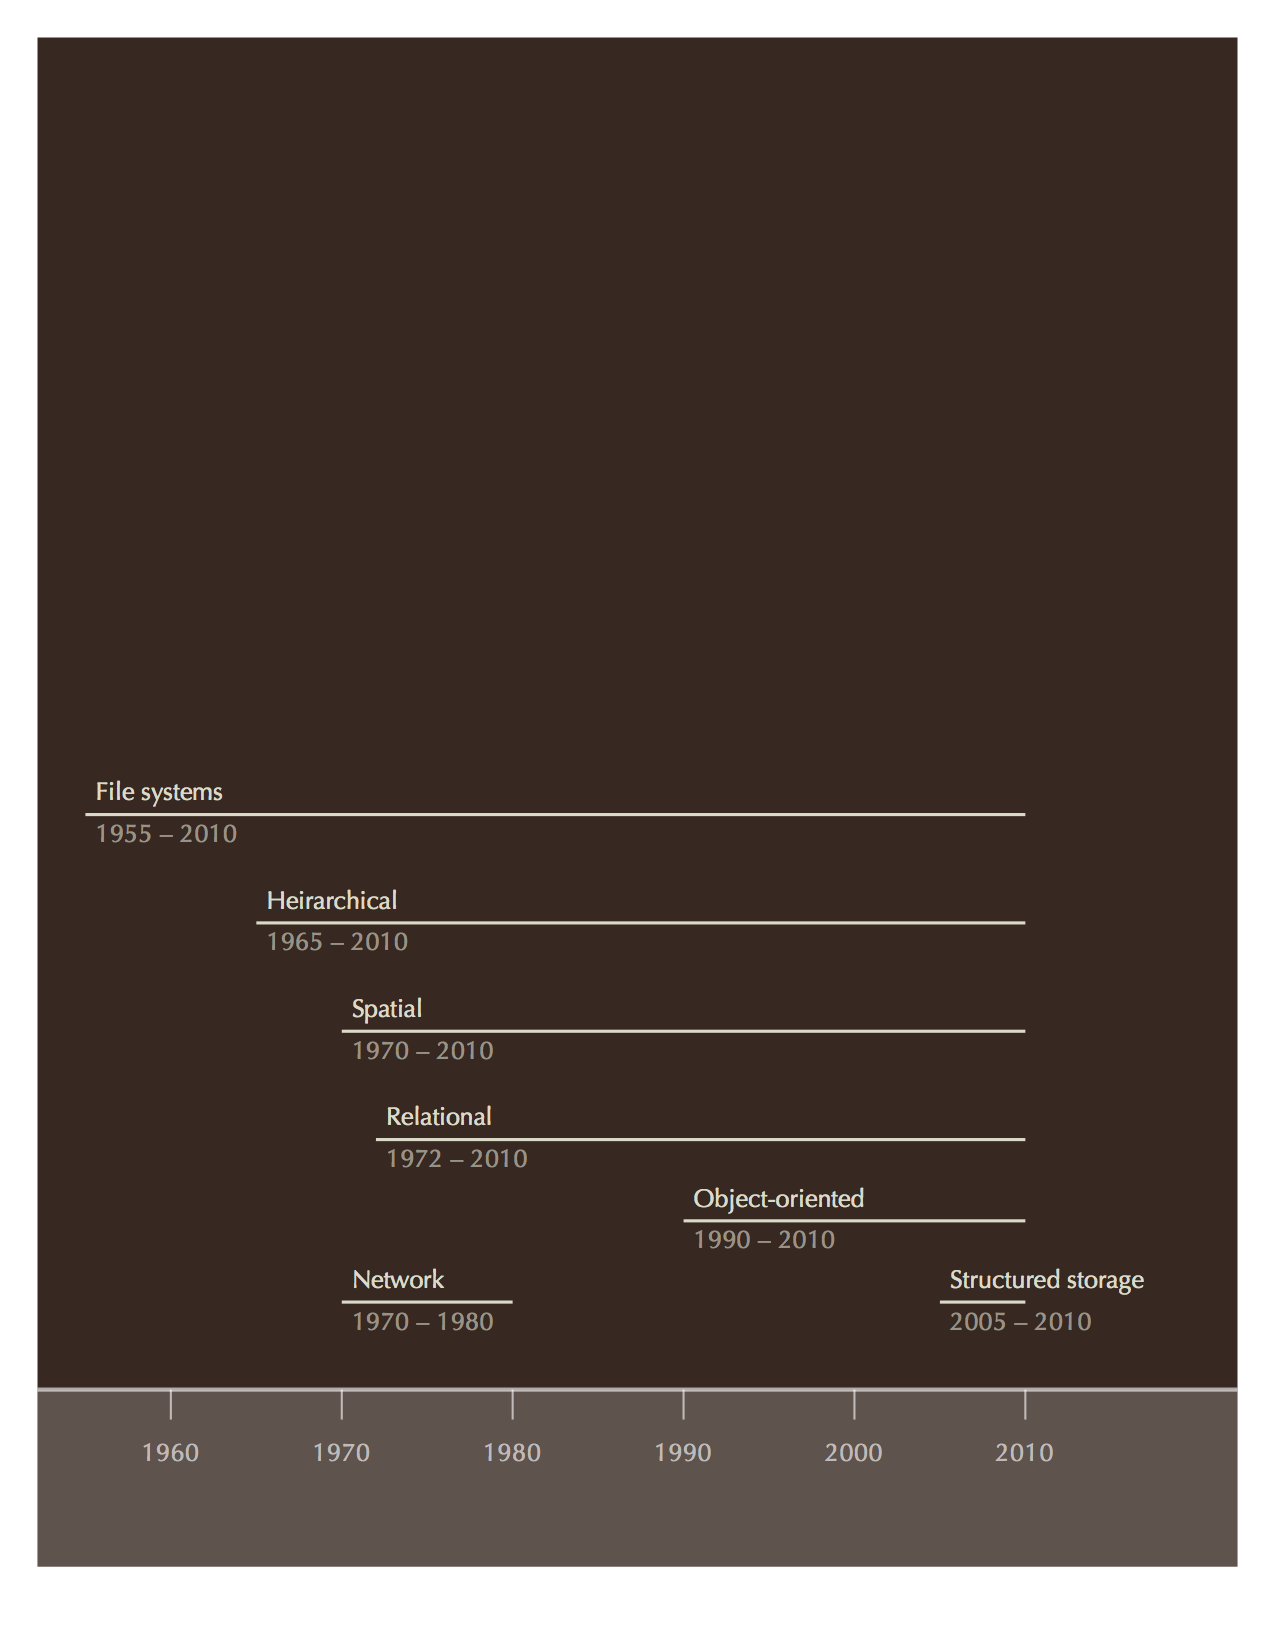
\includegraphics{Figures/Chapter 1/timeline2.png}

File systems were the earliest form of data management. Limited by the
sequential nature of magnetic tape technology, it was very difficult to
integrate data from different files. The advent of magnetic disk
technology in the mid-1950s stimulated development of integrated file
systems, and the hierarchical database management system (DBMS) emerged
in the 1960s, followed some years later by the network DBMS. The spatial
database, or geographic information system (GIS), appeared around 1970.
Until the mid-1990s, the hierarchical DBMS, mainly in the form of IBM's
DL/I product, was the predominant technology for managing data. It has
now been replaced by the relational DBMS, a concept first discussed by
Edgar Frank Codd in an academic paper in 1970 but not commercially
available until the mid-1970s. In the late 1980s, the notion of an
object-oriented DBMS, primed by the ideas of object-oriented
programming, emerged as a solution to situations not handled well by the
relational DBMS. Also around this time, the idea of modeling a database
as a graph was introduced. Towards the end of the 20th century, XML was
developed for exchanging data between computers, and it can also be used
as a data store as you will learn in section 3. More recently,
tdistributed files system, such as Hadoop, have emerged as alternative
models for data management. Other recent data management systems include
graph and NoSQL databases. While these are beyond the scope of an
introductory data management text, if you decided to pursue a career in
data management you should learn about their advantages and the
applications to which they are well-suited. For example, graph databases
are a good fit for the analysis of social networks.

This book concentrates on the relational model, currently the most
widely used data management system. As mentioned, Section 2 is devoted
to the development of the necessary skills for designing and using a
relational database.

\hypertarget{data-information-and-knowledge}{%
\subsection*{Data, information, and knowledge}\label{data-information-and-knowledge}}
\addcontentsline{toc}{subsection}{Data, information, and knowledge}

Often the terms \textbf{\emph{data}} and \textbf{\emph{information}} are used
interchangeably, but they are distinctly different. Data are raw,
unsummarized, and unanalyzed facts. Information is data that have been
processed into a meaningful form.

A list of a supermarket's daily receipts is data, but it is not
information, because it is too detailed to be very useful. A summary of
the data that gives daily departmental totals is information, because
the store manager can use the report to monitor store performance. The
same report might be data for a regional manager, because it is too
detailed for meaningful decision making at the regional level.
Information for a regional manager might be a weekly report of sales by
department for each supermarket.

Data are always data, but one person's information can be another
person's data. Information that is meaningful to one person can be too
detailed for another. A manager's notion of information can change
quickly, however. When a problem is identified, a manager might request
finer levels of detail to diagnose the problem's cause. Thus, what was
previously data suddenly becomes information because it helps solve the
problem. When the problem is solved, the information reverts to data.
There is a need for information systems that let managers customize the
processing of data so that they always get information. As their needs
change, they need to be able to adjust the detail of the reports they
receive.

Knowledge is the capacity to use information. The education and
experience that managers accumulate provide them with the expertise to
make sense of the information they receive. Knowledge means that
managers can interpret information and use it in decision making. In
addition, knowledge is the capacity to recognize what information would
be useful for making decisions. For example, a sales manager might know
that requesting a report of profitability by product line is useful when
she has to decide whether to employ a new product manager. Thus, when a
new information system is delivered, managers need to be taught what
information the system can deliver and what that information means.

The relationship between data, information, and knowledge is depicted in
the following figure. A knowledgeable person requests information to
support decision making. To fulfill the request, data are converted into
information. Personal knowledge is then applied to interpret the
requested information and reach a conclusion. Of course, the cycle can
be repeated several times if more information is needed before a
decision can be made. Notice how knowledge is essential for grasping
what information to request and interpreting that information in terms
of the required decision.

\emph{The relationship between data, information, and knowledge}

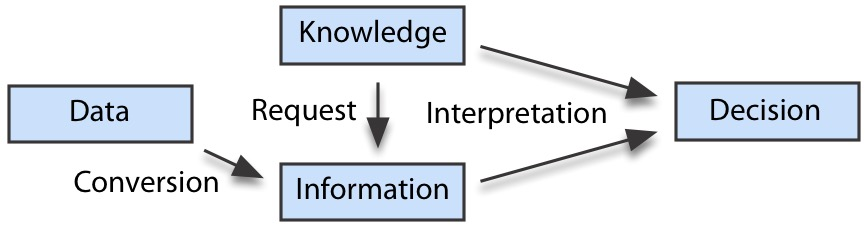
\includegraphics{Figures/Chapter 1/data-info-know.jpg}

\hypertarget{the-challenge}{%
\subsection*{The challenge}\label{the-challenge}}
\addcontentsline{toc}{subsection}{The challenge}

A major challenge facing organizations is to make effective use of the
data currently stored in their diverse data management systems. This
challenge exists because these various systems are not integrated and
many potential clients not only lack the training to access the systems
but often are unaware what data exist. Before data managers can begin to
address this problem, however, they must understand how organizational
memories are used. In particular, they need to understand the
relationship between information and managerial decision making. Data
management is not a new problem. It has existed since the early days of
civilization and will be an enduring problem for organizations and
societies.

\hypertarget{summary}{%
\subsection*{Summary}\label{summary}}
\addcontentsline{toc}{subsection}{Summary}

Organizations must maintain a memory to process transactions and make
decisions. Organizational data should be shareable, transportable,
secure, and accurate, and provide timely, relevant information. The
essential components are people (the most important), text, multimedia
data, models, and knowledge. A wide variety of technologies can be used
to manage data. External memories enlarge the range of data available to
an organization. Data management systems often have some major
shortcomings: redundancy, poor data control, poor interfaces, long lead
times for query resolution, an inability to supply answers for questions
posed by managers, and poor data integration. Data are raw facts;
information is data processed into a meaningful form. Knowledge is the
capacity to use information.

\begin{longtable}[]{@{}ll@{}}
\toprule
Key terms and concepts & \\
\midrule
\endhead
Data & Internal memory \\
Database management system (DBMS) & Knowledge \\
Data management & Machine learning \\
Data mining & Management information system (MIS) \\
Data security & Metamemory \\
Decision making & Online analytical processing (OLAP) \\
Decision quality & Organizational culture \\
Decision support system (DSS) & Organizational memory \\
External memory & Standard operating procedures \\
Geographic information system (GIS) & Tables \\
Information & Transaction processing system (TPS) \\
\bottomrule
\end{longtable}

\hypertarget{references-and-additional-readings}{%
\subsubsection*{References and additional readings}\label{references-and-additional-readings}}
\addcontentsline{toc}{subsubsection}{References and additional readings}

Davenport, T. H. (1998). Putting the enterprise into the enterprise
system. \emph{Harvard Business Review}, 76(4), 121-131.

\hypertarget{exercises}{%
\subsubsection*{Exercises}\label{exercises}}
\addcontentsline{toc}{subsubsection}{Exercises}

\begin{enumerate}
\def\labelenumi{\arabic{enumi}.}
\item
  What are the major differences between internal and external memory?
\item
  What is the difference between the things you remember and the
  things you record on your computer?
\item
  What features are common to most individual memory systems?
\item
  What do you think organizations did before computers were invented?
\item
  Discuss the memory systems you use. How do they improve your
  performance? What are the shortcomings of your existing systems? How
  can you improve them?
\item
  Describe the most ``organized'' person you know. Why is that person so
  organized? Why haven't you adopted some of the same methods? Why do
  you think people differ in the extent to which they are organized?
\item
  Think about the last time you enrolled in a class. What data do you
  think were recorded for this transaction?
\item
  What roles do people play in organizational memory?
\item
  What do you think is the most important attribute of organizational
  memory? Justify your answer.
\item
  What is the difference between transaction processing and decision
  making?
\item
  When are data relevant?
\item
  Give some examples of specialized memories.
\item
  How can you measure the quality of a decision?
\item
  What is organizational culture? Can you name some organizations that
  have a distinctive culture?
\item
  What is hypertext? How does it differ from linear text? Why might
  hypertext be useful in an organizational memory system?
\item
  What is imaging? What are the characteristics of applications well
  suited for imaging?
\item
  What is an external memory? Why do organizations use external
  memories instead of building internal memories?
\item
  What is the common name used to refer to systems that help
  organizations remember knowledge?
\item
  What is a DSS? What is its role in organizational memory?
\item
  What are the major shortcomings of many data management systems?
  Which do you think is the most significant shortcoming?
\item
  What is the relationship between data, information, and knowledge?
\item
  Estimate how much data Netflix requires to store its many movies.
\item
  Using the Web, find some stories about firms using data management
  systems. You might enter keywords such as ``database'' and ``business
  analytics'' and access the sites of publications such as
  \href{http://www.computerworld.com/}{\underline{Computerworld}}. Identify the
  purpose of each system. How does the system improve organizational
  performance? What are the attributes of the technology that make it
  useful? Describe any trade-offs the organization might have made.
  Identify other organizations in which the same technology might be
  applied.
\item
  Make a list of the organizational memory systems identified in this
  chapter. Interview several people working in organizations. Ask them
  to indicate which organizational memory systems they use. Ask which
  system is most important and why. Write up your findings and your
  conclusion.
\end{enumerate}

\newpage

\hypertarget{information}{%
\section{Information}\label{information}}

\begin{quote}
\emph{Effective information management must begin by thinking about how
people use information---not with how people use machines.}

Davenport, T. H. (1994). Saving IT's soul: human-centered information
management. \emph{Harvard Business Review,} 72(2), 119-131.
\end{quote}

\hypertarget{learning-objectives-1}{%
\subsection*{Learning objectives}\label{learning-objectives-1}}
\addcontentsline{toc}{subsection}{Learning objectives}

Students completing this chapter will

\begin{itemize}
\item
  understand the importance of information to society and
  organizations;
\item
  be able to describe the various roles of information in
  organizational change;
\item
  be able to distinguish between soft and hard information;
\item
  know how managers use information;
\item
  be able to describe the characteristics of common information
  delivery systems;
\item
  distinguish the different types of knowledge.
\end{itemize}

\hypertarget{introduction-1}{%
\subsection*{Introduction}\label{introduction-1}}
\addcontentsline{toc}{subsection}{Introduction}

There are three characteristics of the early decades of the twenty-first
century: global warming, high-velocity global change, and the emerging
power of information organizations.\footnote{In mid 2017, the five most valuable public companies were Apple,
  Google, Amazon, Microsoft, and Facebook. Furthermore, they are
  concentrated on the west coast of the U.S. in either Silicon Valley
  or Seattle.} The need to create a sustainable
civilization, the globalization of business, and the rise of China as a
major economic power are major forces contributing to mass change.
Organizations are undergoing large-scale restructuring as they attempt
to reposition themselves to survive the threats and exploit the
opportunities presented by these changes.

In the last few years, some very powerful and highly profitable
information-based organizations have emerged. Apple and MS vie to be the
world's largest company in terms of market value. Leveraging the iPhone
and IOS, Apple has shown the power of information services to change an
industry. Google has become a well-known global brand as it fulfills its
mission ``to organize the world's information and make it universally
accessible and useful.'' Amazon is disrupting traditional retail.
Facebook has digitized our social world, and Microsoft has dominated the
office environment for decades. We gain further insights into the value
of information by considering its role in civilization.

\hypertarget{a-historical-perspective}{%
\subsection*{A historical perspective}\label{a-historical-perspective}}
\addcontentsline{toc}{subsection}{A historical perspective}

Humans have been collecting data to manage their affairs for several
thousand years. In 3000 BCE, Mesopotamians recorded inventory details in
cuneiform, an early script. Today's society transmits Exabytes of data
every day as billions of people and millions of organizations manage
their affairs. The dominant issue facing each type of economy has
changed over time, and the collection and use of data has changed to
reflect these concerns, as shown in the following table.

\emph{Societal focus}

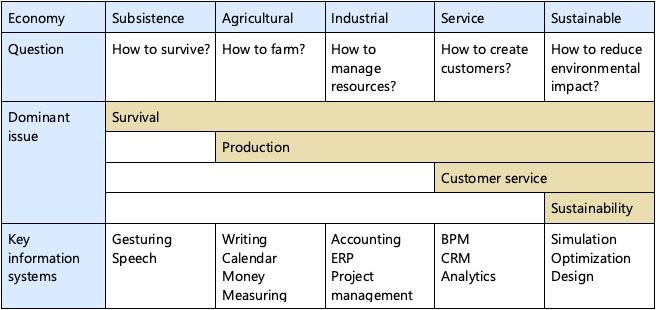
\includegraphics{Figures/Chapter 2/societal focus.png}

Agrarian society was concerned with productive farming, and an important
issue was when to plant crops. Ancient Egypt, for example, based its
calendar on the flooding of the Nile. The focus shifted during the
industrial era to management of resources (e.g., raw materials, labor,
logistics). Accounting, ERP, and project management became key
information systems for managing resources. In the current service
economy, the focus has shifted to customer creation. There is an
oversupply of many consumer products (e.g., cars) and companies compete
to identify services and product features that will attract customers.
They are concerned with determining what types of customers to recruit
and finding out what they want. As a result, we have seen the rise of
business analytics and customer relationship management (CRM) to address
this dominant issue. As well as creating customers, firms need to serve
those already recruited. High quality service often requires frequent
and reliable execution of multiple processes during manifold encounters
with customers by a firm's many customer facing employees (e.g., a fast
food store, an airline, a hospital). Consequently, business process
management (BPM) has grown in importance since the mid 1990s when there
was a surge of interest in business process reengineering.

We are in transition to a new era, sustainability, where attention
shifts to assessing environmental impact because, after several
centuries of industrialization, atmospheric CO\textsubscript{2} levels have become
alarmingly high. We are also reaching the limits of the planet's
resources as its population now exceeds seven billion people. As a
result, a new class of application is emerging, such as environmental
management systems and UPS's telematics project.\footnote{Watson, R. T., Boudreau, M.-C., Li, S., \& Levis, J. (2010).
  Telematics at UPS: En route to Energy Informatics. MISQ Executive,
  9(1), 1-11.} These new systems
will also include, for example, support for understanding environmental
impact through simulation of energy consuming and production systems,
optimization of energy systems, and design of low impact production and
customer service systems. Notice that dominant issues don't disappear
but rather aggregate in layers, so tomorrow's business will be concerned
with survival, production, customer service, and sustainability. As a
result, a firm's need for data never diminishes, and each new layer
creates another set of data needs. The flood will not subside and for
most firms the data flow will need to grow significantly to meet the new
challenge of sustainability.

A constant across all of these economies is organizational memory, or in
its larger form, social memory. Writing and paper manufacturing
developed about the same time as agricultural societies. Limited writing
systems appeared about 30,000 years ago. Full writing systems, which
have evolved in the last 5,000 years, made possible the technological
transfer that enabled humanity to move from hunting and gathering to
farming. Writing enables the recording of knowledge, and information can
accumulate from one generation to the next. Before writing, knowledge
was confined by the limits of human memory.

There is a need for a technology that can store knowledge for extended
periods and support transport of written information. Storage medium has
advanced from clay tablets (4000 BCE), papyrus (3500 BCE), and parchment
(2000 BCE) to paper (100 CE.). Written knowledge gained great impetus
from Johannes Gutenberg, whose achievement was a printing system
involving movable metal type, ink, paper, and press. In less than 50
years, printing technology diffused throughout most of Europe. In the
last century, a range of new storage media appeared (e.g., photographic,
magnetic, and optical).

Organizational memories emerged with the development of large
organizations such as governments, armies, churches, and trading
companies. The growth of organizations during the industrial revolution
saw a massive increase in the number and size of organizational
memories. This escalation continued throughout the twentieth century.

The Internet has demonstrated that we now live in a borderless world.
There is a free flow of information, investment, and industry across
borders. Customers ignore national boundaries to buy products and
services. In the borderless information age, the old ways of creating
wealth have been displaced by intelligence, marketing, global reach, and
education. Excelling in the management of data, information, and
knowledge has become a prerequisite to corporate and national wealth.

\emph{Wealth creation}

\begin{longtable}[]{@{}ll@{}}
\toprule
The old & The new \\
\midrule
\endhead
Military power & Intelligence \\
Natural resources & Marketing \\
Population & Global reach \\
Industry & Education \\
\bottomrule
\end{longtable}

This brief history shows the increasing importance of information.
Civilization was facilitated by the discovery of means for recording and
disseminating information. In our current society, organizations are the
predominant keepers and transmitters of information.

\hypertarget{a-brief-history-of-information-systems}{%
\subsection*{A brief history of information systems}\label{a-brief-history-of-information-systems}}
\addcontentsline{toc}{subsection}{A brief history of information systems}

Information systems has three significant eras. In the first era,
information work was transported to the computer. For instance, a
punched card deck was physically transported to a computer center, the
information was processed, and the output physically returned to the
worker as a printout.

\emph{Information systems eras}

\begin{longtable}[]{@{}
  >{\raggedright\arraybackslash}p{(\columnwidth - 8\tabcolsep) * \real{0.07}}
  >{\raggedright\arraybackslash}p{(\columnwidth - 8\tabcolsep) * \real{0.18}}
  >{\raggedright\arraybackslash}p{(\columnwidth - 8\tabcolsep) * \real{0.18}}
  >{\raggedright\arraybackslash}p{(\columnwidth - 8\tabcolsep) * \real{0.18}}
  >{\raggedright\arraybackslash}p{(\columnwidth - 8\tabcolsep) * \real{0.18}}@{}}
\toprule
E
ra & Focus & Period & Technology & Networks \\
\midrule
\endhead
1 & Take
i
nformation
work to
the
computer & 1950s ---
mid-1970s & Batch & Few data
networks \\
2 & Take
i
nformation
work to
the
employee & \begin{minipage}[t]{\linewidth}\raggedright
\hypertarget{mid-1970s}{%
\subsection{Mid-1970s}\label{mid-1970s}}

mid-1990s
\end{minipage} & H
ost/termin
al

Cli
ent/server & Spread of
private
networks \\
3 & Take
i
nformation
work to
the
customer
and other
st
akeholders & \begin{minipage}[t]{\linewidth}\raggedright
\hypertarget{mid-1990s}{%
\subsection{Mid-1990s}\label{mid-1990s}}

present
\end{minipage} & Brow
ser/server & \vtop{\hbox{\strut Public
networks}\hbox{\strut (Internet)}} \\
\bottomrule
\end{longtable}

In the second era, private networks were used to take information work
to the employee. Initially, these were time-sharing and host/terminal
systems. IS departments were concerned primarily with creating systems
for use by an organization's employees when interacting with customers
(e.g., a hotel reservation system used by call center employees) or for
the employees of another business to transact with the organization
(e.g., clerks in a hospital ordering supplies).

Era 3 starts with the appearance of the Web browser in the mid-1990s.
The browser, which can be used on the public and global Internet,
permits organizations to take information and information work to
customers and other stakeholders. Now, the customer undertakes work
previously done by the organization (e.g., making an airline
reservation).

The scale and complexity of era 3 is at least an order of magnitude
greater than that of era 2. Nearly every company has far more customers
than employees. For example, UPS, with an annual investment of more than
\$1 billion in information technology and over 400,000 employees, is one
of the world's largest employers. However, there are 11 million
customers, over 25 times the number of employees, who are today
electronically connected to UPS.

Era 3 introduced direct electronic links between a firm and its
stakeholders, such as investors and citizens. In the earlier eras,
intermediaries often communicated with stakeholders on behalf of the
firm (e.g., a press release to the news media). These messages could be
filtered and edited, or sometimes possibly ignored, by intermediaries.
Now, organizations can communicate directly with their stakeholders via
the Web, e-mail, social media. Internet technologies offer firms a
chance to rethink their goals vis-à-vis each stakeholder class and to
use Internet technology to pursue these goals.

This brief history leads to the conclusion that the value IS creates is
determined by whom an organization can reach, how it can reach them, and
where and when it can reach them.

\begin{itemize}
\item
  \textbf{Whom}. Whom an organization can contact determines whom it can
  influence, inform, or transfer work to. For example, if a hotel can
  be contacted electronically by its customers, it can promote online
  reservations (transfer work to customers), and reduce its costs.
\item
  \textbf{How}. How an organization reaches a stakeholder determines the
  potential success of the interaction. The higher the bandwidth of
  the connection, the richer the message (e.g., using video instead of
  text), the greater the amount of information that can be conveyed,
  and the more information work that can be transferred.
\item
  \textbf{Where}. Value is created when customers get information directly
  related to their current location (e.g., a navigation system) and
  what local services they want to consume (e.g., the nearest Italian
  restaurant).
\item
  \textbf{When}. When a firm delivers a service to a client can greatly
  determine its value. Stockbrokers, for instance, who can inform
  clients immediately of critical corporate news or stock market
  movements are likely to get more business.
\end{itemize}

\hypertarget{information-characteristics}{%
\subsection*{Information characteristics}\label{information-characteristics}}
\addcontentsline{toc}{subsection}{Information characteristics}

Three useful concepts for describing information are hardness, richness,
and class. Information hardness is a subjective measure of the accuracy
and reliability of an item of information. Information richness
describes the concept that information can be rich or lean depending on
the information delivery medium. Information class groups types of
information by their key features.

\hypertarget{information-hardness}{%
\subsection*{Information hardness}\label{information-hardness}}
\addcontentsline{toc}{subsection}{Information hardness}

In 1812, the Austrian mineralogist Friedrich Mohs proposed a scale of
hardness, in order of increasing relative hardness, based on 10 common
minerals. Each mineral can scratch those with the same or a lower
number, but cannot scratch higher-numbered minerals.

A similar approach can be used to describe information. Market
information, such as the current price of gold, is the hardest because
it is measured extremely accurately. There is no ambiguity, and its
measurement is highly reliable. In contrast, the softest information,
which comes from unidentified sources, is rife with uncertainty.

\emph{An information hardness scale}

\begin{longtable}[]{@{}
  >{\raggedright\arraybackslash}p{(\columnwidth - 4\tabcolsep) * \real{0.15}}
  >{\centering\arraybackslash}p{(\columnwidth - 4\tabcolsep) * \real{0.10}}
  >{\raggedright\arraybackslash}p{(\columnwidth - 4\tabcolsep) * \real{0.68}}@{}}
\toprule
Mineral & S
cale & Data \\
\midrule
\endhead
Talc & 1 & Unidentified source---rumors, gossip, and
hearsay \\
Gypsum & 2 & Identified non-expert source---opinions,
feelings, and ideas \\
Calcite & 3 & Identified expert source---predictions,
speculations, forecasts, and estimates \\
Fluorite & 4 & Unsworn testimony---explanations,
justifications, assessments, and
interpretations \\
Apatite & 5 & Sworn testimony---explanations,
justifications, assessments, and
interpretations \\
Or
thoclase & 6 & Budgets, formal plans \\
Quartz & 7 & News reports, non-financial data, industry
statistics, and surveys \\
Topaz & 8 & Unaudited financial statements, and government
statistics \\
Corundum & 9 & Audited financial statements \\
Diamond & 1 0 & Stock exchange and commodity market data \\
\bottomrule
\end{longtable}

Audited financial statements are in the corundum zone. They are measured
according to standard rules (known as ``generally accepted accounting
principles'') that are promulgated by national accounting societies.
External auditors monitor the application of these standards, although
there is generally some leeway in their application and sometimes
multiple standards for the same item. The use of different accounting
principles can lead to different profit and loss statements. As a
result, the information in audited financial statements has some degree
of uncertainty.

There are degrees of hardness within accounting systems. The hardest
data are counts, such as units sold or customers served. These are
primary measures of organizational performance. Secondary measures, such
as dollar sales and market share, are derived from counts. Managers vary
in their preference for primary and secondary measures. Operational
managers opt for counts for measuring productivity because they are
uncontaminated by price changes and currency fluctuations. Senior
managers, because their focus is on financial performance, select
secondary measures.

The scratch test provides a convenient and reliable method of assessing
the hardness of a mineral. Unfortunately, there is no scratch test for
information. Managers must rely on their judgment to assess information
hardness.

Although managers want hard information, there are many cases when it is
not available. They compensate by seeking information from several
different sources. Although this approach introduces redundancy, this is
precisely what the manager seeks. Relatively consistent information from
different sources is reassuring.

\hypertarget{information-richness}{%
\subsection*{Information richness}\label{information-richness}}
\addcontentsline{toc}{subsection}{Information richness}

Information can be described as rich or lean. It is richest when
delivered face-to-face. Conversation permits immediate feedback for
verification of meaning. You can always stop the other speaker and ask,
``What do you mean?'' Face-to-face information delivery is rich because
you see the speaker's body language, hear the tone of voice, and natural
language is used. A numeric document is the leanest form of information.
There is no opportunity for questions, no additional information from
body movements and vocal tone. The information richness of some
communication media is shown in the following table.

\emph{Information richness and communication media}\footnote{\emph{Daft, R. L., \& Lengel, R. H. (1986). Organizational information
  requirements, media richness, and structural design. Management
  Science}, 32(5), 554-571.}

\begin{longtable}[]{@{}
  >{\raggedright\arraybackslash}p{(\columnwidth - 8\tabcolsep) * \real{0.17}}
  >{\raggedright\arraybackslash}p{(\columnwidth - 8\tabcolsep) * \real{0.17}}
  >{\raggedright\arraybackslash}p{(\columnwidth - 8\tabcolsep) * \real{0.17}}
  >{\raggedright\arraybackslash}p{(\columnwidth - 8\tabcolsep) * \real{0.22}}
  >{\raggedright\arraybackslash}p{(\columnwidth - 8\tabcolsep) * \real{0.17}}@{}}
\toprule
Richest & & & & Leanest \\
\midrule
\endhead
Fac
e-to-face & Telephone & Personal
documents & Impersonal
written
documents & Numeric
documents \\
\bottomrule
\end{longtable}

Managers seek rich information when they are trying to resolve
equivocality or ambiguity. It means that managers cannot make sense of a
situation because they arrive at multiple, conflicting interpretations
of the information. An example of an equivocal situation is a class
assignment where some of the instructions are missing and others are
contradictory (of course, this example is an extremely rare event).

Equivocal situations cannot be resolved by collecting more information,
because managers are uncertain about what questions to ask and often a
clear answer is not possible. Managers reduce equivocality by sharing
their interpretations of the available information and reaching a
collective understanding of what the information means. By exchanging
opinions and recalling their experiences, they try to make sense of an
ambiguous situation.

Many of the situations that managers face each day involve a high degree
of equivocality. Formal organizational memories, such as databases, are
not much help, because the information they provide is lean. Many
managers rely far more on talking with colleagues and using informal
organizational memories such as social networks.

Data management is almost exclusively concerned with administering the
formal information systems that deliver lean information. Although this
is their proper role, data managers must realize that they can deliver
only a portion of the data required by decision makers.

\hypertarget{information-classes}{%
\subsection*{Information classes}\label{information-classes}}
\addcontentsline{toc}{subsection}{Information classes}

Information can be grouped into four classes: content, form, behavior,
and action. Until recently, most organizational information fell into
the first category.

\emph{Information classes}

\begin{longtable}[]{@{}
  >{\raggedright\arraybackslash}p{(\columnwidth - 2\tabcolsep) * \real{0.15}}
  >{\raggedright\arraybackslash}p{(\columnwidth - 2\tabcolsep) * \real{0.83}}@{}}
\toprule
Class & Description \\
\midrule
\endhead
Content & Quantity, location, and types of items \\
Form & Shape and composition of an object \\
Behavior & Simulation of a physical object \\
Action & Creation of action (e.g., industrial robots) \\
\bottomrule
\end{longtable}

Content information records details about quantity, location, and types
of items. It tends to be historical in nature and is traditionally the
class of information collected and stored by organizations. The content
information of a car would describe its model number, color, price,
options, horsepower, and so forth. Hundreds of bytes of data may be
required to record the full content information of a car. Typically,
content data are captured by a TPS.

Form information describes the shape and composition of an object. For
example, the form information of a car would define the dimensions and
composition of every component in the car. Millions of bytes of data are
needed to store the form of a car. CAD/CAM systems are used to create
and store form information.

Behavior information is used to predict the behavior of a physical
object using simulation techniques, which typically require form
information as input. Massive numbers of calculations per second are
required to simulate behavior. For example, simulating the flight of a
new aircraft design may require trillions of computations. Behavior
information is often presented visually because the vast volume of data
generated cannot be easily processed by humans in other formats.

Action information enables the instantaneous creation of sophisticated
action. Industrial robots take action information and manufacture parts,
weld car bodies, or transport items. Antilock brakes are an example of
action information in use.

\hypertarget{information-and-organizational-change}{%
\subsection*{Information and organizational change}\label{information-and-organizational-change}}
\addcontentsline{toc}{subsection}{Information and organizational change}

Organizations are goal-directed. They undergo continual change as they
use their resources, people, technology, and financial assets to reach
some future desired outcome. Goals are often clearly stated, such as to
make a profit of \$100 million, win a football championship, or decrease
the government deficit by 25 percent in five years. Goals are often not
easily achieved, however, and organizations continually seek information
that supports goal attainment. The information they seek falls into
three categories: goal setting, gap, and change.

\emph{Organizational information categories}

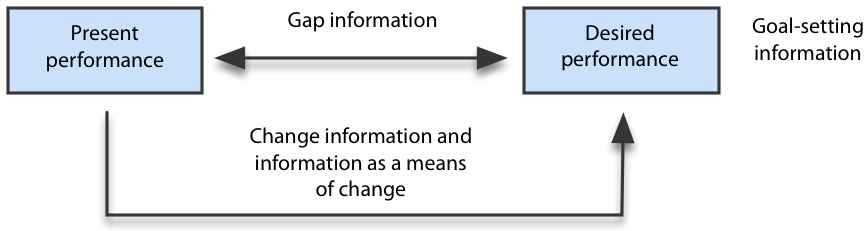
\includegraphics{Figures/Chapter 2/gap model.jpg}

The emergence of an information society also means that information
provides dual possibilities for change. Information is used to plan
change, and information is a medium for change.

\hypertarget{goal-setting-information}{%
\subsection*{Goal-setting information}\label{goal-setting-information}}
\addcontentsline{toc}{subsection}{Goal-setting information}

Organizations set goals or levels of desired performance. Managers need
information to establish goals that are challenging but realistic. A
common approach is to take the previous goal and stretch it. For
example, a company with a 15 percent return on investment (ROI) might
set the new goal at 17 percent ROI. This technique is known as
``anchoring and adjusting.'' Prior performance is used as a basis for
setting the new performance standards. The problem with anchoring and
adjusting is that it promotes incremental improvement rather than
radical change because internal information is used to set performance
standards. Some organizations have turned to external information and
are using benchmarking as a source of information for goal setting.

\hypertarget{planning}{%
\subsubsection*{Planning}\label{planning}}
\addcontentsline{toc}{subsubsection}{Planning}

Planning is an important task for senior managers. To set the direction
for the company, they need information about consumers' potential
demands and social, economic, technical, and political conditions. They
use this information to determine the opportunities and threats facing
the organization, thus permitting them to take advantage of
opportunities and avoid threats.

Most of the information for long-term planning comes from sources
external to the company. There are think tanks that analyze trends and
publish reports on future conditions. Journal articles and books can be
important sources of information about future events. There also will be
a demand for some internal information to identify trends in costs and
revenues. Major planning decisions, such as building a new plant, will
be based on an analysis of internal data (use of existing capacity) and
external data (projected customer demand).

\hypertarget{benchmarking}{%
\subsubsection*{Benchmarking}\label{benchmarking}}
\addcontentsline{toc}{subsubsection}{Benchmarking}

Benchmarking establishes goals based on best industry practices. It is
founded on the Japanese concept of \emph{dantotsu}, striving to be the best
of the best. Benchmarking is externally directed. Information is sought
on those companies, regardless of industry, that demonstrate outstanding
performance in the areas to be benchmarked. Their methods are studied,
documented, and used to set goals and redesign existing practices for
superior performance.

Other forms of external information, such as demographic trends,
economic forecasts, and competitors' actions can be used in goal
setting. External information is valuable because it can force an
organization to go beyond incremental goal setting.

Organizations need information to identify feasible, motivating, and
challenging goals. Once these goals have been established, they need
information on the extent to which these goals have been attained.

\hypertarget{gap-information}{%
\subsection*{Gap information}\label{gap-information}}
\addcontentsline{toc}{subsection}{Gap information}

Because goals are meant to be challenging, there is often a gap between
actual and desired performance. Organizations use a number of mechanisms
to detect a gap and gain some idea of its size. Problem identification
and scorekeeping are two principal methods of providing gap information.

\hypertarget{problem-identification}{%
\subsubsection*{Problem identification}\label{problem-identification}}
\addcontentsline{toc}{subsubsection}{Problem identification}

Business conditions are continually changing because of competitors'
actions, trends in consumer demand, and government actions. Often these
changes are reflected in a gap between expectations and present
performance. This gap is known as a problem.

To identify problems, managers use exception reports, which are
generated only when conditions vary from the established goal or
standard. Once a potential problem has been identified, managers collect
additional information to confirm that a problem really exists. Once
management has been alerted, the information delivery system needs to
shift into high gear. Managers will request rapid delivery of ad hoc
reports from a variety of sources. The ideal organizational memory
system can adapt smoothly to deliver appropriate information quickly.

\hypertarget{scorekeeping}{%
\subsubsection*{Scorekeeping}\label{scorekeeping}}
\addcontentsline{toc}{subsubsection}{Scorekeeping}

Keeping track of the score provides gap information. Managers ask many
questions: How many items did we make yesterday? What were the sales
last week? Has our market share increased in the last year? They
establish measurement systems to track variables that indicate whether
organizational performance is on target. Keeping score is important;
managers need to measure in order to manage. Also, measurement lets
people know what is important. Once a manager starts to measure
something, subordinates surmise that this variable must be important and
pay more attention to the factors that influence it.

There are many aspects of the score that a manager can measure. The
overwhelming variety of potentially available information is illustrated
by the sales output information that a sales manager could track. Sales
input information (e.g., number of service calls) can also be measured,
and there is qualitative information to be considered. Because of time
constraints, most managers are forced to limit their attention to 10 or
fewer key variables singled out by the critical success factors (CSF)
method.\footnote{Rockart, J.F. (1982). The changing role of the information systems
  executive: a critical success factors perspective. \emph{Sloan Management
  Review}, 24(1), 3-13.} Scorekeeping information is usually fairly stable.

\emph{Sales output tracking information}

\begin{longtable}[]{@{}
  >{\raggedright\arraybackslash}p{(\columnwidth - 2\tabcolsep) * \real{0.21}}
  >{\raggedright\arraybackslash}p{(\columnwidth - 2\tabcolsep) * \real{0.78}}@{}}
\toprule
Category & Example \\
\midrule
\endhead
Orders & Number of current customers \\
& Average order size \\
& Batting average (orders to calls) \\
Sales volume & Dollar sales volume \\
& Unit sales volume \\
& By customer type \\
& By product category \\
& Translated to market share \\
& Quota achieved \\
Margins & Gross margin \\
& Net profit \\
& By customer type \\
& By product \\
Customers & Number of new accounts \\
& Number of lost accounts \\
& Percentage of accounts sold \\
& Number of accounts overdue \\
& Dollar value of receivables \\
& Collections of receivables \\
\bottomrule
\end{longtable}

\hypertarget{change-information}{%
\subsection*{Change information}\label{change-information}}
\addcontentsline{toc}{subsection}{Change information}

Accurate change information is very valuable because it enables managers
to predict the outcome of various actions to close a gap with some
certainty. Unfortunately, change information is usually not very
precise, and there are many variables that can influence the effect of
any planned change. Nevertheless, organizations spend a great deal of
time collecting information to support problem solving and planning.

\hypertarget{problem-solution}{%
\subsection*{Problem solution}\label{problem-solution}}
\addcontentsline{toc}{subsection}{Problem solution}

Once a concern has been identified, a manager seeks to find its cause. A
decrease in sales could be the result of competitors introducing a new
product, an economic downturn, an ineffective advertising campaign, or
many other reasons. Data can be collected to test each of these possible
causes. Additional data are usually required to support analysis of each
alternative. For example, if the sales decrease has been caused by an
economic recession, the manager might use a decision support system
(DSS) to analyze the effect of a price decrease or a range of
promotional activities.

\hypertarget{information-as-a-means-of-change}{%
\subsection*{Information as a means of change}\label{information-as-a-means-of-change}}
\addcontentsline{toc}{subsection}{Information as a means of change}

The emergence of an information society means that information can be
used as a means of changing an organization's performance. Corporations
can create information-based products and services, adding information
to products, and using information to enhance existing performance or
gain a competitive advantage. Further insights into the use of
information as a change agent are gained by examining marketing,
customer service, and empowerment.

\hypertarget{marketing}{%
\subsection*{Marketing}\label{marketing}}
\addcontentsline{toc}{subsection}{Marketing}

Marketing is a key strategy for changing organizational performance by
increasing sales. Information has become an important component in
marketing. Airlines and retailers have established frequent flyer and
buyer programs to encourage customer loyalty and gain more information
about customers. These systems are heavily dependent on database
technology because of the massive volume of data that must be stored.
Indeed, without database technology, some marketing strategies could
never be implemented.

Database technology offers the opportunity to change the very nature of
communications with customers. Broadcast media have been the traditional
approach to communication. Advertisements are aired on television,
placed in magazines, or displayed on a Web site. Database technology can
be used to address customers directly. No longer just a mailing list,
today's database is a memory of customer relationships, a record of
every message and response between the firm and a customer. Some
companies keep track of customers' preferences and customize
advertisements to their needs. Leading online retailers now send
customers only those emails for products for which they estimate there
is a high probability of a purchase. For example, a customer with a
history of buying jazz music is sent an email promoting jazz recordings
instead of one featuring classical music.

The Web has significantly enhanced the value of database technology.
Many firms now use a combination of a Web site and a DBMS to market
products and service customers.

\hypertarget{customer-service}{%
\subsection*{Customer Service}\label{customer-service}}
\addcontentsline{toc}{subsection}{Customer Service}

Many American business leaders rank customer service as their most
important goal for organizational success. Many of the developed
economies are service driven. In the United States, services account for
nearly 80 percent of the GNP and most of the new jobs. Many companies
now compete for customers by offering superior customer service.
Information is frequently a key to this improved service.

\begin{quote}
❓\emph{Skill builder}

For many businesses, information is the key to high-quality customer
service. Thus, some firms use information, and thus customer service,
as a key differentiating factor, while others might compete on price.
Compare the electronics component of Web sites Amazon and Walmart. How
do they use price and information to compete? What are the
implications for data management if a firm uses information to
compete?
\end{quote}

\hypertarget{empowerment}{%
\subsection*{Empowerment}\label{empowerment}}
\addcontentsline{toc}{subsection}{Empowerment}

Empowerment means giving employees greater freedom to make decisions.
More precisely, it is sharing with frontline employees

\begin{itemize}
\item
  information about the organization's performance;
\item
  rewards based on the organization's performance;
\item
  knowledge and information that enable employees to understand and
  contribute to organizational performance;
\item
  power to make decisions that influence organizational direction and
  performance.
\end{itemize}

Notice that information features prominently in the process. A critical
component is giving employees access to the information they need to
perform their tasks with a high degree of independence and discretion.
Information is empowerment. By linking employees to organizational
memory, data managers play a pivotal role in empowering people.
Empowerment can contribute to organizational performance by increasing
the quality of products and services. Together, empowerment and
information are mechanisms of planned change.

\hypertarget{information-and-managerial-work}{%
\subsection*{Information and managerial work}\label{information-and-managerial-work}}
\addcontentsline{toc}{subsection}{Information and managerial work}

Because managers frequently use data management systems in their normal
activities as a source of information about change and as a means of
implementing change, it is crucial for systems designers to understand
how managers work. Failure to take account of managerial behavior can
result in a system that is technically sound but rarely used because it
does not fit the social system.

Studies over several decades reveal a very consistent pattern:
Managerial work is very fragmented. Managers spend an average of 10
minutes on any task, and their day is organized into brief periods of
concentrated attention to a variety of tasks. They work unrelentingly
and are frequently interrupted by unexpected disturbances. Managers are
action oriented and rely on intuition and judgment far more than
contemplative analysis of information.

Managers strongly prefer oral communication. They spend a great deal of
time conversing directly or by telephone. Managers use interpersonal
communication to establish networks, which they later use as a source of
information and a way to make things happen. The continual flow of
verbal information helps them make sense of events and lets them feel
the organizational pulse.

Managers rarely use formal reporting systems. They do not spend their
time analyzing computer reports or querying databases but resort to
formal reports to confirm impressions, should interpersonal
communications suggest there is a problem. Even when managers are
provided with a purpose-built, ultra-friendly executive information
system, their behavior changes very little. They may access a few
screens during the day, but oral communication is still their preferred
method of data gathering and dissemination.

\hypertarget{managers-information-requirements}{%
\subsection*{Managers' information requirements}\label{managers-information-requirements}}
\addcontentsline{toc}{subsection}{Managers' information requirements}

Managers have certain requirements of the information they receive.
These expectations should shape a data management system's content and
how data are processed.

Managers expect to receive information that is useful for their current
task under existing business conditions. Unfortunately, managerial tasks
can change rapidly. The interlinked, global, economic environment is
highly turbulent. Since managers' expectations are not stable, the
information delivery system must be sufficiently flexible to meet
changing requirements.

Managers' demands for information vary with their perception of its
hardness; they require only one source that scores 10 on the information
hardness scale. The Nikkei Index at the close of today's market is the
same whether you read it in the \emph{Asian Wall Street Journal} or \emph{The
Western Australian} or hear it on CNN. As perceived hardness decreases,
managers demand more information, hoping to resolve uncertainty and gain
a more accurate assessment of the situation. When the reliability of a
source is questionable, managers seek confirmation from other sources.
If a number of different sources provide consistent information, a
manager gains confidence in the information's accuracy.

\emph{Relationship of perceived information hardness to volume of information
requested}

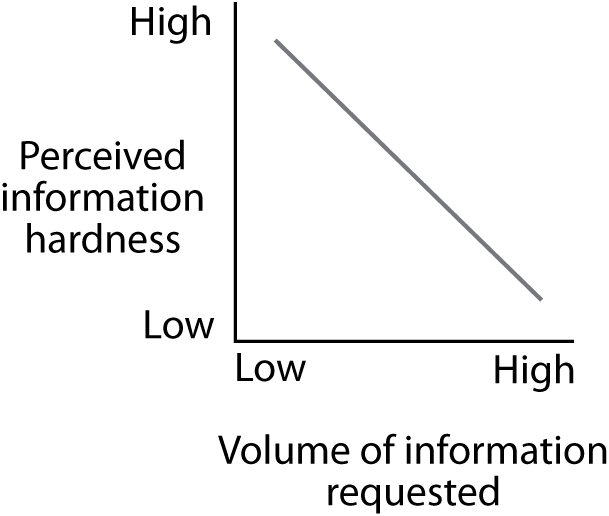
\includegraphics[width=3.16667in,height=\textheight]{Figures/Chapter 2/hardness-volume tradeoff.png}

It is not unusual, therefore, to have a manager seek information from a
database, a conversation with a subordinate, and a contact in another
organization. If a manager gets essentially the same information from
each source, she or he has the confirmation sought. This means each data
management system should be designed to minimize redundancy, but
different components of organizational memory can supply overlapping
information.

\hypertarget{managers-needs-for-information-vary-accordingly-with-responsibilities}{%
\subsection*{Managers' needs for information vary accordingly with responsibilities}\label{managers-needs-for-information-vary-accordingly-with-responsibilities}}
\addcontentsline{toc}{subsection}{Managers' needs for information vary accordingly with responsibilities}

Operational managers need detailed, short-term information to deal with
well-defined problems in areas such as sales, service, and production.
This information comes almost exclusively from internal sources that
report recent performance in the manager's area. A sales manager may get
weekly reports of sales by each direct report.

As managers move up the organizational hierarchy, their information
needs both expand and contract. They become responsible for a wider
range of activities and are charged with planning the future of the
organization, which requires information from external sources on
long-term economic, demographic, political, and social trends. Despite
this long-term focus, top-level managers also monitor short-term,
operational performance. In this instance, they need less detail and
more summary and exception reports on a small number of key indicators.
To avoid information overload as new layers of information needs are
added, the level of detail on the old layers naturally must decline, as
illustrated in the following figure.

\emph{Management level and information need}

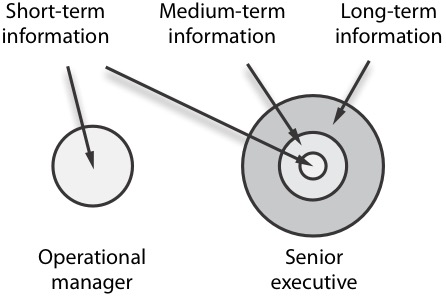
\includegraphics{Figures/Chapter 2/onion model.jpg}

\hypertarget{information-satisficing}{%
\subsection*{Information satisficing}\label{information-satisficing}}
\addcontentsline{toc}{subsection}{Information satisficing}

Because managers face making many decisions in a short period, most do
not have the time or resources to collect and interpret all the
information they need to make the best decision. Consequently, they are
often forced to satisfice. That is, they accept the first satisfactory
decision they discover. They also satisfice in their information search,
collecting only enough information to make a satisfactory decision.

Ultimately, information satisficing leads to lower-quality decision
making. If, however, information systems can accelerate delivery and
processing of the right information, then managers should be able to
move beyond selecting the first satisfactory decision to selecting the
best of several satisfactory decisions.

\hypertarget{information-delivery-systems}{%
\subsection*{Information delivery systems}\label{information-delivery-systems}}
\addcontentsline{toc}{subsection}{Information delivery systems}

Most organizations have a variety of delivery systems to provide
information to managers. Developed over many years, these systems are
integrated, usually via a Web site, to give managers better access to
information. There are two aspects to information delivery. First, there
is a need for software that accesses an organizational memory, extracts
the required data, and formats it for presentation. We can use the
categories of organizational memories introduced in Chapter 1 to
describe the software side of information delivery systems. The second
aspect of delivery is the hardware that gets information from a computer
to the manager.

\emph{Information delivery systems software}

\begin{longtable}[]{@{}
  >{\raggedright\arraybackslash}p{(\columnwidth - 2\tabcolsep) * \real{0.33}}
  >{\raggedright\arraybackslash}p{(\columnwidth - 2\tabcolsep) * \real{0.65}}@{}}
\toprule
Organizational memory & Delivery systems \\
\midrule
\endhead
People & Conversation \\
& E-mail \\
& Meeting \\
& Report \\
& Groupware \\
Files & Management information system (MIS) \\
Documents & Web browser \\
& E-mail attachment \\
Images & Image processing system (IPS) \\
Graphics & Computer aided design (CAD) \\
& Geographic information system (GIS) \\
Voice & Voice mail \\
& Voice recording system \\
Mathematical model & Decision support system (DSS) \\
Decisions & Conversation \\
& E-mail \\
& Meeting \\
& Report \\
& Groupware \\
\bottomrule
\end{longtable}

Software is used to move data to and from organizational memory. There
is usually tight coupling between software and the format of an
organizational memory. For example, a relational database management
system can access tables but not decision-support models. This tight
coupling is particularly frustrating for managers who often want
integrated information from several organizational memories. For
example, a sales manager might expect a monthly report to include
details of recent sales (from a relational database) to be combined with
customer comments (from email messages to a customer service system). A
quick glance at the preceding table shows that there are many different
information delivery systems. We will discuss each of these briefly to
illustrate the lack of integration of organizational memories.

\hypertarget{verbal-exchange}{%
\subsubsection*{Verbal exchange}\label{verbal-exchange}}
\addcontentsline{toc}{subsubsection}{Verbal exchange}

Conversations, meetings, and oral reporting are commonly used methods of
information delivery. Indeed, managers show a strong preference for
verbal exchange as a method for gathering information. This is not
surprising because we are accustomed to oral information. This is the
way we learned for thousands of years as a preliterate culture. Only
recently have we learned to make decisions using spreadsheets and
computer reports.

\hypertarget{voice-mail}{%
\subsubsection*{Voice mail}\label{voice-mail}}
\addcontentsline{toc}{subsubsection}{Voice mail}

Voice mail is useful for people who do not want to be interrupted. It
supports asynchronous communication; that is, the two parties to the
conversation are not simultaneously connected. Voice-mail systems also
can store many prerecorded messages that can be selectively replayed
using a phone's keypad. Organizations use this feature to support
standard customer queries.

\hypertarget{electronic-mail}{%
\subsubsection*{Electronic mail}\label{electronic-mail}}
\addcontentsline{toc}{subsubsection}{Electronic mail}

Email is an important system of information delivery. It too supports
asynchronous messaging, and it is less costly than voice mail for
communication. Many documents are exchanged as attachments to email.

\hypertarget{formal-report}{%
\subsubsection*{Formal report}\label{formal-report}}
\addcontentsline{toc}{subsubsection}{Formal report}

Formal reports have a long history in organizations. Before electronic
communication, they were the main form of information delivery. They
still have a role in organizations because they are an effective method
of integrating information of varying hardness and from a variety of
organizational memories. For example, a report can contain text, tables,
graphics, and images.

Formal reports are often supplemented by a verbal presentation of the
key points in the report. Such a presentation enhances the information
delivered, because the audience has an opportunity to ask questions and
get an immediate response.

\hypertarget{meetings}{%
\subsubsection*{Meetings}\label{meetings}}
\addcontentsline{toc}{subsubsection}{Meetings}

Because managers spend 30-80 percent of their time in meetings, these
are a key source of information.

\hypertarget{groupware}{%
\subsubsection*{Groupware}\label{groupware}}
\addcontentsline{toc}{subsubsection}{Groupware}

Since meetings occupy so much managerial time and in many cases are
poorly planned and managed, organizations are looking for improvements.
Groupware is a general term applied to a range of software systems
designed to improve some aspect of group work. It is excellent for
tapping soft information and the informal side of organizational memory.

\hypertarget{management-information-system}{%
\paragraph*{Management information system}\label{management-information-system}}
\addcontentsline{toc}{paragraph}{Management information system}

Management information systems are a common method of delivering
information from data management systems. A preplanned query is often
used to extract the data. Managers who have developed some skills in
using a query language might create custom reports as needed.

Preplanned reports often contain too much or too detailed information,
because they are designed in anticipation of a manager's needs.
Customized reports do not have these shortcomings, but they are often
more expensive and time consuming because they need to be prepared by an
analyst.

\hypertarget{web}{%
\paragraph*{Web}\label{web}}
\addcontentsline{toc}{paragraph}{Web}

Word processing, desktop publishing, or HTML editors are used for
preparing documents that are disseminated by placing them on a Web
server for convenient access and sharing.

\hypertarget{image-processing-system}{%
\paragraph*{Image processing system}\label{image-processing-system}}
\addcontentsline{toc}{paragraph}{Image processing system}

An image processing system (IPS) captures data using a scanner to
digitize an image. Images in the form of letters, reports,
illustrations, and graphics have always been an important type of
organizational memory. An IPS permits these forms of information to be
captured electronically and disseminated.

\hypertarget{computer-aided-design}{%
\paragraph*{Computer-aided design}\label{computer-aided-design}}
\addcontentsline{toc}{paragraph}{Computer-aided design}

Computer-aided design (CAD) is used extensively to create graphics. For
example, engineers use CAD in product design, and architects use it for
building design. These plans are a part of organizational memory for
designers and manufacturers.

\hypertarget{geographic-information-system}{%
\paragraph*{Geographic information system}\label{geographic-information-system}}
\addcontentsline{toc}{paragraph}{Geographic information system}

Many cities uses a geographic information system (GIS) to store
graphical data about roads, utilities, and services. This information is
another form of organizational memory.

\hypertarget{decision-support-system}{%
\paragraph*{Decision support system}\label{decision-support-system}}
\addcontentsline{toc}{paragraph}{Decision support system}

A decision support system (DSS) is frequently a computer-based
mathematical model of a problem. DSS software, available in a range of
packages, permits the model and data to be retrieved and executed. Model
parameters can be varied to investigate alternatives.

\hypertarget{information-integration}{%
\subsection*{Information integration}\label{information-integration}}
\addcontentsline{toc}{subsection}{Information integration}

A fundamental problem for most organizations is that their memory is
fragmented across a wide variety of formats and technologies. Too
frequently, there is a one-to-one correspondence between an
organizational memory for a particular functional area and the software
delivery system. For example, sales information is delivered by the
sales system and production information by the production system. This
is not a very desirable situation because managers want all the
information they need, regardless of its source or format, amalgamated
into a single report.

A common solution is to develop software, such as a Web application,
that integrates information from a variety of delivery systems. An
important task of this apl is to integrate and present information from
multiple organizational memories. Recently, some organizations have
created vast integrated data stores---data warehouses--- that are
organized repositories of organizational data.

\emph{Information integration - the present situation}

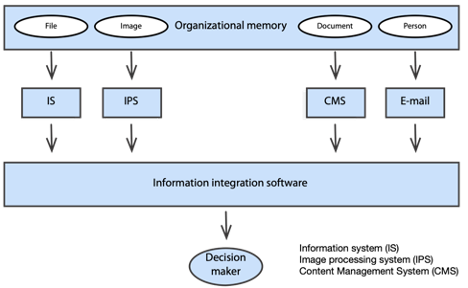
\includegraphics{Figures/Chapter 2/fragmented memory.png}

\emph{The ideal organizational memory and information delivery system}

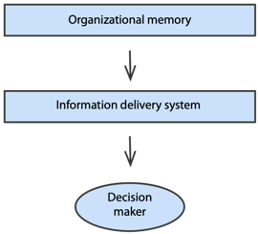
\includegraphics{Figures/Chapter 2/integrated memory.png}

\hypertarget{knowledge-1}{%
\subsection*{Knowledge}\label{knowledge-1}}
\addcontentsline{toc}{subsection}{Knowledge}

The performance of many organizations is determined more by their
cognitive capabilities and knowledge than their physical assets. A
nation's wealth is increasingly a result of the knowledge and skills of
its citizens, rather than its natural resources and industrial plants.
Currently, about 85 percent of all jobs in America and 80 percent of
those in Europe are knowledge-based.

An organization's knowledge, in order of increasing importance, is

\begin{itemize}
\item
  cognitive knowledge (know what);
\item
  advanced skills (know how);
\item
  system understanding and trained intuition (know why);
\item
  self-motivated creativity (care why).
\end{itemize}

This text illustrates the different types of knowledge. You will develop
cognitive knowledge in Section 4, when you learn about data
architectures and implementations. For example, knowing what storage
devices can be used for archival data is cognitive knowledge. Section 2,
data modeling and SQL, develops advanced skills because, upon completion
of that section, you will know how to model data and write SQL queries.
The first two chapters expand your understanding of the influence of
organizational memory on organizational performance. You need to know
why you should learn data management skills. Managers know when and why
to apply technology, whereas technicians know what to apply and how to
apply it. Finally, you are probably an IS major, and your coursework is
inculcating the values and norms of the IS profession so that you care
why problems are solved using information technology.

Organizations tend to spend more on developing cognitive skills than
they do on fostering creativity. This is, unfortunately, the wrong
priority. Returns are likely to be much greater when higher-level
knowledge skills are developed. Well-managed organizations place more
attention on creating know why and care why skills because they
recognize that knowledge is a key competitive weapon. Furthermore, these
firms have learned that knowledge grows, often very rapidly, when
shared. Knowledge is like a communication network whose potential
benefit grows exponentially as the nodes within the network grow
arithmetically. When knowledge is shared within the organization, or
with customers and suppliers, it multiplies as each person receiving
knowledge imparts it to someone else in the organization or a business
partner.

\emph{Skills values vs.~training expenditures (Quinn et al., 1996)}

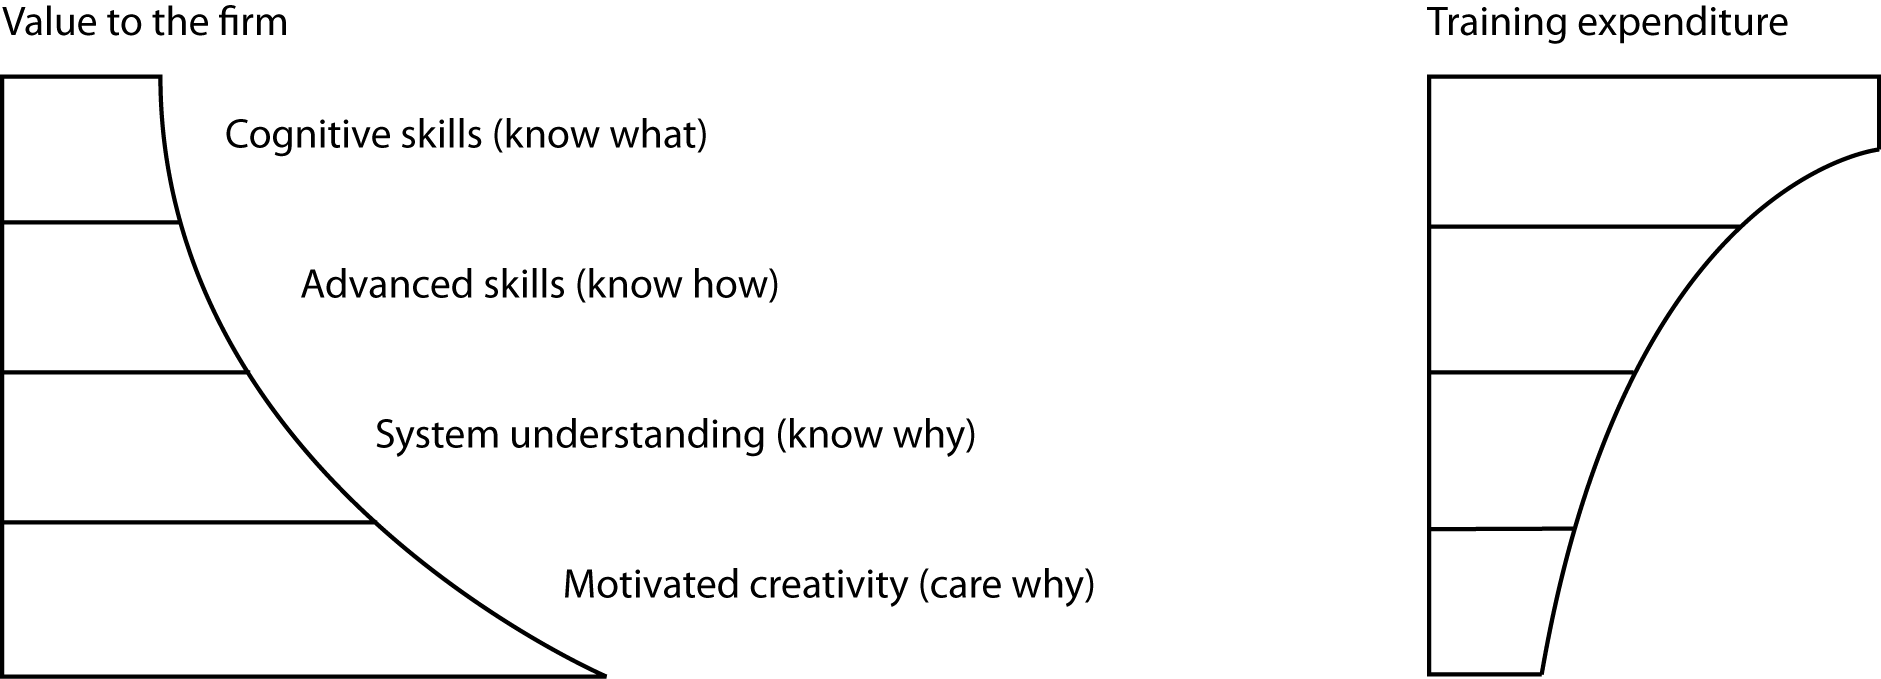
\includegraphics{Figures/Chapter 2/knowledge and training.png}

There are two types of knowledge: explicit and tacit. Explicit knowledge
is codified and transferable. This textbook is an example of explicit
knowledge. Knowledge about how to design databases has been formalized
and communicated with the intention of transferring it to you, the
reader. Tacit knowledge is personal knowledge, experience, and judgment
that is difficult to codify. It is more difficult to transfer tacit
knowledge because it resides in people's minds. Usually, the transfer of
tacit knowledge requires the sharing of experiences. In learning to
model data, the subject of the next section, you will quickly learn how
to represent an entity, because this knowledge is made explicit.
However, you will find it much harder to model data, because this skill
comes with practice. Ideally, you should develop several models under
the guidance of an experienced modeler, such as your instructor, who can
pass on his or her tacit knowledge.

\hypertarget{summary-1}{%
\subsection*{Summary}\label{summary-1}}
\addcontentsline{toc}{subsection}{Summary}

Information has become a key foundation for organizational growth. The
information society is founded on computer and communications
technology. The accumulation of knowledge requires a capacity to encode
and share information. Hard information is very exact. Soft information
is extremely imprecise. Rich information exchange occurs in face-to-face
conversation. Numeric reports are an example of lean information.
Organizations use information to set goals, determine the gap between
goals and achievements, determine actions to reach goals, and create new
products and services to enhance organizational performance. Managers
depend more on informal communication systems than on formal reporting
systems. They expect to receive information that meets their current,
ever changing needs. Operational managers need short-term information.
Senior executives require mainly long-term information but still have a
need for both short- and medium-term information. When managers face
time constraints, they collect only enough information to make a
satisfactory decision. Organizational memory should be integrated to
provide one interface to an organization's information stores.

\begin{longtable}[]{@{}ll@{}}
\toprule
Key terms and concepts & \\
\midrule
\endhead
Advanced skills (know how) & Information organization \\
Benchmarking & Information requirements \\
Change information & Information richness \\
Cognitive knowledge (know what) & Information satisficing \\
Empowerment & Information society \\
Explicit knowledge & Knowledge \\
Gap information & Managerial work \\
Global change & Organizational change \\
Goal-setting information & Phases of civilization \\
Information as a means of change & Self-motivated creativity (care why) \\
Information delivery systems & Social memory \\
Information hardness & System understanding (know why) \\
Information integration & Tacit knowledge \\
\bottomrule
\end{longtable}

\hypertarget{references-and-additional-readings-1}{%
\subsection*{References and additional readings}\label{references-and-additional-readings-1}}
\addcontentsline{toc}{subsection}{References and additional readings}

Quinn, J. B., P. Anderson, and S. Finkelstein. 1996. Leveraging
intellect. \emph{Academy of Management Executive} 10 (3):7-27.

\hypertarget{exercises-1}{%
\subsection*{Exercises}\label{exercises-1}}
\addcontentsline{toc}{subsection}{Exercises}

\begin{enumerate}
\def\labelenumi{\arabic{enumi}.}
\item
  From an information perspective, what is likely to be different
  about the customer service era compared to the forthcoming
  sustainability era?
\item
  How does an information job differ from an industrial job?
\item
  Why was the development of paper and writing systems important?
\item
  What is the difference between soft and hard information?
\item
  What is the difference between rich and lean information exchange?
\item
  What are three major types of information connected with
  organizational change?
\item
  What is benchmarking? When might a business use benchmarking?
\item
  What is gap information?
\item
  Give some examples of how information is used as a means of change.
\item
  What sorts of information do senior managers want?
\item
  Describe the differences between the way managers handle hard and
  soft information.
\item
  What is information satisficing?
\item
  Describe an incident where you used information satisficing.
\item
  Give some examples of common information delivery systems.
\item
  What is a GIS? Who might use a GIS?
\item
  Why is information integration a problem?
\item
  How ``hard'' is an exam grade?
\item
  Could you develop a test for the hardness of a piece of information?
\item
  Is very soft information worth storing in formal organizational
  memory? If not, where might you draw the line?
\item
  If you had just failed your database exam, would you use rich or
  lean media to tell a parent or spouse about the result?
\item
  Interview a businessperson to determine his or her firm's critical
  success factors (CSFs). Remember, a CSF is something the firm must
  do right to be successful. Generally a firm has about seven CSFs.
  For the firm's top three CSFs, identify the information that will
  measure whether the CSF is being achieved.
\item
  If you were managing a fast-food store, what information would you
  want to track store performance? Classify this information as
  short-, medium-, or long-term.
\item
  Interview a manager. Identify the information that person uses to
  manage the company. Classify this information as short-, medium-, or
  long-term information. Comment on your findings.
\item
  Why is organizational memory like a data warehouse? What needs to be
  done to make good use of this data warehouse?
\item
  What information are you collecting to help determine your career or
  find a job? What problems are you having collecting this
  information? Is the information mainly hard or soft?
\item
  What type of knowledge should you gain in a university class?
\item
  What type of knowledge is likely to make you most valuable?
\end{enumerate}

\newpage

\hypertarget{section-2-data-modeling-and-sql}{%
\section*{Section 2 Data Modeling and SQL}\label{section-2-data-modeling-and-sql}}
\addcontentsline{toc}{section}{Section 2 Data Modeling and SQL}

\begin{quote}
\emph{It is a capital mistake to theorize before one has data.}

Sir Arthur Conan Doyle, ``A Scandal in Bohemia,'' \emph{The Adventures of
Sherlock Holmes}, 1891
\end{quote}

The application backlog, a large number of requests for new information
systems, has been a recurring problem in many organizations for decades.
The demand for new information systems and the need to maintain existing
systems have usually outstripped available information systems skills.
The application backlog, unfortunately, is not a new problem. In the
1970s, Codd laid out a plan for improving programmer productivity and
accelerating systems development by improving the management of data.
Codd's \textbf{relational model}, designed to solve many of the shortcomings
of earlier systems, is currently the most popular database model.

This section develops two key skills---data modeling and query
formation---that are required to take advantage of the relational model.
We concentrate on the design and use of relational databases. This very
abrupt change in focus is part of the plan to give you a dual
understanding of data management. Section 1 is the managerial
perspective, whereas this section covers technical skills development.
Competent data managers are able to accommodate both views and apply
whichever (or some blend of the two) is appropriate.

In Chapter 1, many forms of organizational memory were identified, and
in this section we focus on files and their components. Thus, only the
files branch of organizational memory is detailed in the following
figure.

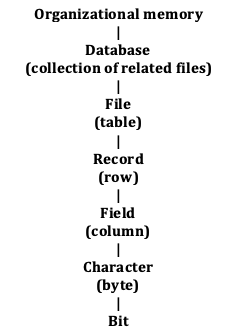
\includegraphics{Figures/Section 2/Org Memory Files.png}

A collection of related files is a \textbf{database}. Describing the
collection of files as related means that it has a common purpose (e.g.,
data about students). Sometimes files are also called tables, and there
are synonyms for some other terms (the alternative names are shown in
parentheses). Files contain \textbf{records} (or rows). Each record contains
the data for one instance of the data the file stores. For example, if
the file stores data about students, each record will contain data about
a single student. Records have \textbf{fields} (or columns) that store the
fine detail of each instance (e.g., student's first name, last name, and
date of birth). Fields are composed of \textbf{characters} (a, b, c,.., 1,
2, 3,\ldots, \%, \$, \#,\ldots, A, B, etc.). A \textbf{byte}, a unit of
storage sufficient to store a single letter (in English) or digit,
consists of a string of eight contiguous \textbf{bits} or binary digits.

The data management hierarchy stimulates three database design
questions:

\begin{itemize}
\item
  What collection of files should the database contain?
\item
  How are these files related?
\item
  What fields should each record in the file contain?
\end{itemize}

The first objective of this section is to describe data modeling, a
technique for answering the three questions. Data modeling helps you to
understand the structure and meaning of data, which is necessary before
a database can be created. Once a database has been designed, built, and
loaded with data, the aim is to deploy it to satisfy management's
requests for information. Thus, the second objective is to teach you to
query a relational database. The learning of modeling and querying will
be intertwined, making it easier to grasp the intent of database design
and to understand why data modeling is so critical to making a database
an effective tool for managerial decision making.

Chapter 3 covers modeling a single entity and querying a single-table
database. This is the simplest database that can be created. As you will
soon discover, a \textbf{data model} is a graphical description of the
components of a database. One of these components is an entity, some
feature of the real world about which data must be stored. This section
also introduces the notions of a \textbf{data definition language} (DDL),
which is used to describe a database, and a \textbf{data manipulation
language} (DML), which is used to maintain and query a database.
Subsequent chapters in this section cover advanced data modeling
concepts and querying capabilities.

\hypertarget{the-single-entity}{%
\section{The Single Entity}\label{the-single-entity}}

\begin{quote}
\emph{I want to be alone.}

Attributed to Greta Garbo
\end{quote}

\hypertarget{learning-objectives-2}{%
\subsubsection*{Learning Objectives}\label{learning-objectives-2}}
\addcontentsline{toc}{subsubsection}{Learning Objectives}

Students completing this chapter will be able to

\begin{itemize}
\item
  model a single entity;
\item
  define a single database;
\item
  write queries for a single-table database.
\end{itemize}

\hypertarget{the-relational-model}{%
\subsection*{The relational model}\label{the-relational-model}}
\addcontentsline{toc}{subsection}{The relational model}

The relational model introduced by Codd in 1970 is the most popular technology for managing large collections of data. In this chapter, the major concepts of the relational model are introduced. Extensive coverage of the relational model is left until Chapter 8, by which time you will have sufficient practical experience to appreciate fully its usefulness, value, and elegance.

A \textbf{relation}, similar to the mathematical concept of a set, is a two-dimensional table arranged in rows and columns. This is a very familiar idea. You have been using tables for many years. A \textbf{relational database} is a collection of relations, where \textbf{relation} is a mathematical term for a table. One row of a table stores details of one observation, instance, or case of an item about which facts are retained---for example, one row for details of a particular student. All the rows in a table store data about the same type of item. Thus, a database might have one table for student data and another table for class data. Similarly, each column in the table contains the same type of data. For example, the first column might record a student's identification number. A key database design question is to decide what to store in each table. What should the rows and columns contain?

In a relational database, each row must be uniquely identified. There must be a \textbf{primary key}, such as student identifier, so that a particular row can be designated. The use of unique identifiers is very common. Telephone numbers and e-mail addresses are examples of unique identifiers. Selection of the primary key, or unique identifier, is another key issue of database design.

\begin{quote}
💠 \textbf{Global legal entity identifier (LEI)}

There is no global standard for identifying legal entities across markets and jurisdictions. The need for such a standard was amplified by Lehman Brothers collapse in 2008. Lehman had 209 registered subsidiaries, legal entities, in 21 countries, and it was party to more than 900,000 derivatives contracts upon its collapse. Key stakeholders, such as financial regulators and Lehman's creditors, were unable to assess their exposure. Furthermore, others were unable to assess the possible ripple on them of the effects of the collapse because of the transitive nature of many investments (i.e., A owes B, B owes C, and C owes D).

The adoption of a global legal entity identifier (LEI), should improve financial system regulation and corporate risk management. Regulators will find it easier to monitor and analyze threats to financial stability and risk managers will be more able evaluate their companies' risks.

Source: \url{http://www.ny.frb.org/research/epr/2014/1403flem.pdf}
\end{quote}

The tables in a relational database are \textbf{connected} or \textbf{related} by means of the data in the tables. You will learn, in the next chapter, that this connection is through a pair of values---a primary key and a foreign key. Consider a table of airlines serving a city. When examining this table, you may not recognize the code of an airline, so you then go to another table to find the name of the airline. For example, if you inspect the following table, you find that AM is an international airline serving Atlanta.

\emph{International airlines serving Atlanta}

\begin{longtable}[]{@{}l@{}}
\toprule
Airline \\
\midrule
\endhead
AM \\
JL \\
KX \\
LM \\
MA \\
OS \\
RG \\
SN \\
SR \\
LH \\
LY \\
\bottomrule
\end{longtable}

If you don't know which airline has the abbreviation AM, then you need to look at the following table of airline codes to discover that AeroMexico, with code AM, serves Atlanta. The two tables are related by airline code. Later, you will discover which is the primary key and which is the foreign key.

\emph{A partial list of airline codes}

\begin{longtable}[]{@{}ll@{}}
\toprule
Code & Airline \\
\midrule
\endhead
AA & American Airlines \\
AC & Air Canada \\
AD & Lone Star Airlines \\
AE & Mandarin Airlines \\
AF & Air France \\
AG & Interprovincial Airlines \\
AI & Air India \\
AM & AeroMexico \\
AQ & Aloha Airlines \\
\bottomrule
\end{longtable}

When designing the relational model, Codd provided commands for processing multiple records at a time. His intention was to increase the productivity of programmers by moving beyond the record-at-a-time processing that is found in most programming languages. Consequently, the relational model supports set processing (multiple records-at-a-time), which is most frequently implemented as \textbf{Structured Query Language (SQL).}\footnote{Officially pronounced as ``S-Q-L,'' but often also pronounced as ``sequel''.}

The relational model separates the logical design of a database from its physical storage. This notion of \textbf{data independence} simplifies data modeling and database programming. In this section, we focus on logical database design, and now that you have had a brief introduction to the relational model, you are ready to learn data modeling.

\hypertarget{getting-started}{%
\subsection*{Getting started}\label{getting-started}}
\addcontentsline{toc}{subsection}{Getting started}

As with most construction projects, building a relational database must be preceded by a design phase. Data modeling, our design technique, is a method for creating a plan or blueprint of a database. The data model must accurately mirror real-world relationships if it is to support processing business transactions and managerial decision making.

Rather than getting bogged down with a \emph{theory first, application later} approach to database design and use, we will start with application. We will get back to theory when you have some experience in data modeling and database querying. After all, you did not learn to talk by first studying sentence formation; you just started by learning and using simple words. We start with the simplest data model, a single entity, and the simplest database, a single table, as follows.

\begin{longtable}[]{@{}llrrrr@{}}
\toprule
Firm code & Firm's name & Price & Quantity & Dividend & PE ratio \\
\midrule
\endhead
FC & Freedonia Copper & 27.5 & 10,529 & 1.84 & 16 \\
PT & Patagonian Tea & 55.25 & 12,635 & 2.50 & 10 \\
AR & Abyssinian Ruby & 31.82 & 22,010 & 1.32 & 13 \\
SLG & Sri Lankan Gold & 50.37 & 32,868 & 2.68 & 16 \\
ILZ & Indian Lead \& Zinc & 37.75 & 6,390 & 3.00 & 12 \\
BE & Burmese Elephant & 0.07 & 154,713 & 0.01 & 3 \\
BS & Bolivian Sheep & 12.75 & 231,678 & 1.78 & 11 \\
NG & Nigerian Geese & 35.00 & 12,323 & 1.68 & 10 \\
CS & Canadian Sugar & 52.78 & 4,716 & 2.50 & 15 \\
ROF & Royal Ostrich Farms & 33.75 & 1,234,923 & 3.00 & 6 \\
\bottomrule
\end{longtable}

\hypertarget{modeling-a-single-entity-database}{%
\subsection*{Modeling a single-entity database}\label{modeling-a-single-entity-database}}
\addcontentsline{toc}{subsection}{Modeling a single-entity database}

The simplest database contains information about one entity, which is some real-world thing. Some entities are physical---CUSTOMER, ORDER, and STUDENT; others are conceptual---WORK ASSIGNMENT and AUTHORSHIP. We represent an entity by a rectangle: the following figure shows a representation of the entity SHARE. The name of the entity is shown in singular form in uppercase in the top part of the rectangle.

\emph{The entity SHARE}


\includegraphics[width=1.58333in,height=\textheight]{Figures/Chapter 3/share.png}

An entity has characteristics or attributes. An \textbf{attribute} is a discrete element of data; it is not usually broken down into smaller components. Attributes identify data we want to store. Some attributes of the entity SHARE are \emph{identification code}, \emph{firm name}, \emph{price}, \emph{quantity owned}, \emph{dividend}, and \emph{price-to-earnings ratio}.\footnote{Attributes are shown in italics.} Attributes are shown below the entity's name. Notice that we refer to \emph{share price}, rather than \emph{price}, to avoid confusion if there should be another entity with an attribute called \emph{price}. Attribute names must be carefully selected so that they are self-explanatory and unique. For example, \emph{share dividend} is easily recognized as belonging to the entity SHARE.

\emph{The entity SHARE and its attributes}

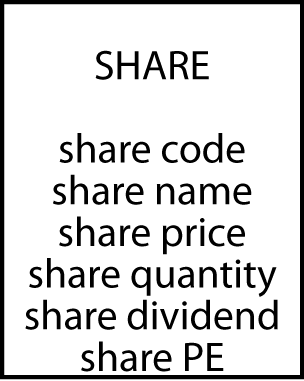
\includegraphics[width=1.58333in,height=\textheight]{Figures/Chapter 3/share with attributes.png}

An \textbf{instance} is a particular occurrence of an entity (e.g., facts about Freedonia Copper). To avoid confusion, each instance of an entity needs to be uniquely identified. Consider the case of customer billing. In most cases, a request to bill Smith \$100 cannot be accurately processed because a firm might have more than one Smith in its customer file. If a firm has carefully controlled procedures for ensuring that each customer has a unique means of identification, then a request to bill customer number 1789 \$100 can be accurately processed. An attribute or collection of attributes that uniquely identifies an instance of an entity is called an \textbf{identifier}. The identifier for the entity SHARE is \emph{share code}, a unique identifier assigned by the stock exchange.

There may be several attributes, or combinations of attributes, that are feasible identifiers for an instance of an entity. Attributes that are identifiers are prefixed by an asterisk. The following figure shows an example of a representation of an entity, its attributes, and identifier.

\emph{The entity SHARE, its attributes, and identifier}

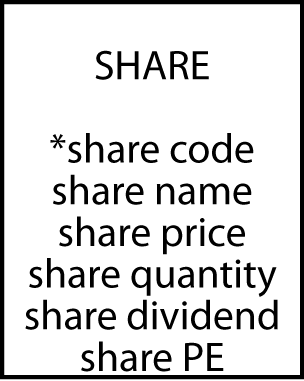
\includegraphics[width=1.58333in,height=\textheight]{Figures/Chapter 3/share with identifier.png}

Briefly, entities are things in the environment about which we wish to store information. Attributes describe an entity. An entity must have a unique identifier.

The modeling language used in this text is designed to record the essential details of a data model. The number of modeling symbols to learn is small, and they preserve all the fundamental concepts of data modeling. Since data modeling often occurs in a variety of settings, the symbols used have been selected so that they can be quickly drawn using pencil-and-paper, whiteboard, or a general-purpose drawing program. This also means that models can be quickly revised as parts can be readily erased and redrawn.

The symbols are distinct and visual clutter is minimized because only the absolutely essential information is recorded. This also makes the language easy for clients to learn so they can read and amend models.

Models can be rapidly translated to a set of tables for a relational database. More importantly, since this text implements the fundamental notions of all data modeling languages, you can quickly convert to another data modeling dialect. Data modeling is a high-level skill, and the emphasis needs to be on learning to think like a data modeler rather than on learning a modeling language. This text's goal is to get you off to a fast start.

\begin{quote}
❓\emph{Skill builder} A ship has a name, registration code, gross tonnage, and a year of construction. Ships are classified as cargo or passenger. Draw a data model for a ship.
\end{quote}

\hypertarget{creating-a-single-table-database}{%
\subsection*{Creating a single-table database}\label{creating-a-single-table-database}}
\addcontentsline{toc}{subsection}{Creating a single-table database}

The next stage is to translate the data model into a relational database. The translation rules are very direct:

\begin{itemize}
\item
  Each entity becomes a table.
\item
  The entity name becomes the table name.
\item
  Each attribute becomes a column.
\item
  The identifier becomes the primary key.
\end{itemize}

The American National Standards Institute's (ANSI) recommended language for relational database definition and manipulation is SQL, which is both a data definition language (DDL) (to define a database), a data manipulation language (DML) (to query and maintain a database), and a data control language (DCL) (to control access). SQL is a common standard for describing and querying databases and is available with many commercial relational database products, including DB2, Oracle, and Microsoft SQL Server, and open source products such as MySQL and PostgreSQL.

In this book, MySQL is the relational database for teaching SQL. Because SQL is a standard, it does not matter which implementation of the relational model you use as the SQL language is common across both the proprietary and open variants.\footnote{Now would be a good time to install the MySQL Community server \url{http:www.mysql.com/downloads/mysql/} on your computer, unless your instructor has set up a class server.} SQL uses the CREATE\footnote{SQL keywords are shown in uppercase.} statement to define a table. It is not a particularly friendly command, and most products have friendlier interfaces for defining tables. However, it is important to learn the standard, because this is the command that SQL understands. Also, a table definition interface will generate a CREATE statement for execution by SQL. Your interface interactions ultimately translate into a standard SQL command.

It is common practice to abbreviate attribute names, as is done in the following example.

\hypertarget{defining-a-table}{%
\paragraph*{Defining a table}\label{defining-a-table}}
\addcontentsline{toc}{paragraph}{Defining a table}

The CREATE command to establish a table called \texttt{share} is as follows:

\begin{Shaded}
\begin{Highlighting}[]
\KeywordTok{CREATE} \KeywordTok{TABLE} \KeywordTok{share}\NormalTok{ (}
\NormalTok{  shrcode }\DataTypeTok{CHAR}\NormalTok{(}\DecValTok{3}\NormalTok{),}
\NormalTok{  shrfirm }\DataTypeTok{VARCHAR}\NormalTok{(}\DecValTok{20}\NormalTok{) }\KeywordTok{NOT} \KeywordTok{NULL}\NormalTok{,}
\NormalTok{  shrprice }\DataTypeTok{DECIMAL}\NormalTok{(}\DecValTok{6}\NormalTok{,}\DecValTok{2}\NormalTok{),}
\NormalTok{  shrqty }\DataTypeTok{DECIMAL}\NormalTok{(}\DecValTok{8}\NormalTok{),}
\NormalTok{  shrdiv }\DataTypeTok{DECIMAL}\NormalTok{(}\DecValTok{5}\NormalTok{,}\DecValTok{2}\NormalTok{),}
\NormalTok{  shrpe }\DataTypeTok{DECIMAL}\NormalTok{(}\DecValTok{2}\NormalTok{),}
  \KeywordTok{PRIMARY} \KeywordTok{KEY}\NormalTok{ (shrcode));}
\end{Highlighting}
\end{Shaded}

The first line of the command names the table; subsequent lines describe each of its columns. The first component is the name of the column (e.g., \texttt{shrcode}). The second component is the data type (e.g., CHAR), and its length is shown in parentheses. \texttt{shrfirm} is a variable-length character field of length 20, which means it can store up to 20 characters, including spaces. The column \texttt{shrdiv} stores a decimal number that can be as large as 999.99 because its total length is 5 digits and there are 2 digits to the right of the decimal point. Some examples of allowable data types are shown in the following table. The third component (e.g., NOT NULL), which is optional, indicates any instance that cannot have null values. A column might have a null value when it is either unknown or not applicable. In the case of the share table, we specify that \texttt{shrfirm} must be defined for each instance in the database.

The final line of the CREATE statement defines \texttt{shrcode} as the primary key, the unique identifier for SHARE When a primary key is defined, the relational database management system (RDBMS) will enforce the requirement that the primary key is unique and not null. Before any row is added to the table SHARE, the RDBMS will check that the value of \texttt{shrcode} is not null and that there does not already exist a duplicate value for \texttt{shrcode} in an existing row of \texttt{share}. If either of these constraints is violated, the RDBMS will not permit the new row to be inserted. This constraint, the \textbf{entity integrity rule}, ensures that every row has a unique, non-null primary key. Allowing the primary key to take a null value would mean there could be a row of \texttt{share} that is not uniquely identified. Note that an SQL statement is terminated by a semicolon, though this is not always enforced.

SQL statements can be written in any mix of valid upper and lowercase characters. To make it easier for you to learn the syntax, this book adopts the following conventions:

\begin{itemize}
\item
  SQL keywords are in uppercase.
\item
  Table and column names are in lowercase.
\end{itemize}

There are more elaborate layout styles, but we will bypass those because it is more important at this stage to learn SQL. You should lay out your SQL statements so that they are easily read by you and others.

The following table shows some of the data types supported by most relational databases. Other implementations of the relational model may support some of these data types and additional ones. It is a good idea to review the available data types in your RDBMS before defining your first table.

\emph{Some allowable data types}

\begin{longtable}[]{@{}
  >{\raggedright\arraybackslash}p{(\columnwidth - 4\tabcolsep) * \real{0.07}}
  >{\raggedright\arraybackslash}p{(\columnwidth - 4\tabcolsep) * \real{0.17}}
  >{\raggedright\arraybackslash}p{(\columnwidth - 4\tabcolsep) * \real{0.76}}@{}}
\toprule
Category & Data type & Description \\
\midrule
\endhead
Numeric & SMALLINT & A 15-bit signed binary value \\
& INTEGER & A 31-bit signed binary value \\
& FLOAT(p) & A scientific format number of p binary digits precision \\
& DECIMAL(p,q) & A packed decimal number of p digits total length; q decimal spaces to the right of the decimal point may be specified \\
String & CHAR(n) & A fixed-length string of n characters \\
& VARCHAR(n) & A variable-length string of up to n characters \\
& TEXT & A variable-length string of up to 65,535 characters \\
Date/time & DATE & Date in the form yyyymmdd \\
& TIME & Time in the form hhmmss \\
& DATETIME & A combination of date and time in the form yyyymmdd hhmmss \\
& TIMESTAMP & A combination of date and time to the nearest microsecond \\
& TIMESTAMP WITH TIME ZONE & Same as timestamp, with the addition of an offset from universal time coordinated (UTC) of the specified time \\
Logical & BOOLEAN & A set of truth values: TRUE, FALSE, or UNKNOWN \\
\bottomrule
\end{longtable}

The CHAR and VARCHAR data types are similar but differ in the way character strings are stored and retrieved. Both can be up to 255 characters long. The length of a CHAR column is fixed to the declared length. When values are stored, they are right-padded with spaces to the specified length. When CHAR values are retrieved, trailing spaces are removed. VARCHAR columns store variable-length strings and use only as many characters as are needed to store the string. Values are not padded; instead, trailing spaces are removed. In this book, we use VARCHAR to define most character strings, unless they are short (less than five characters is a good rule-of-thumb).

\hypertarget{data-modeling-with-mysql-workbench}{%
\subsubsection*{Data modeling with MySQL Workbench}\label{data-modeling-with-mysql-workbench}}
\addcontentsline{toc}{subsubsection}{Data modeling with MySQL Workbench}

MySQL Workbench is a professional quality, open source, cross-platform tool for data modeling and SQL querying.\footnote{\url{http://wb.mysql.com/}} In this text, you will also learn some of the features of Workbench that support data modeling and using SQL. You will find it helpful to complete the MySQL Workbench tutorial on creating a data model\footnote{\url{http://dev.mysql.com/doc/workbench/en/wb-getting-started-tutorial-creating-a-model.html}} prior to further reading, as we will assume you have such proficiency.

\emph{The entity share created with MySQL Workbench}

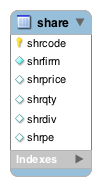
\includegraphics{Figures/Chapter 3/share-wb.png}

You will notice some differences from the data model we have created previously. Workbench automatically generates the SQL code to create the table, so when modeling you establish the names you want for tables and columns. A gold key symbol is used to indicate the identifier, which becomes the primary key. An open diamond indicates that a column can be null, whereas a closed blue diamond indicate the column must have a value, as with \texttt{shrfirm} in this case.

When specifying columns in Workbench you must also indicate the datatype. We opt to turn off the display of a column's datatype\footnote{Preferences \textgreater{} Diagram \textgreater{} Show Column Types} in a model to maintain focus on the entity.

A major advantage of using a tool such as Workbench is that it will automatically generate the CREATE statement code (Database \textgreater{} Forward Engineer \ldots) and execute the code to create the database. The Workbench tutorial will have shown you how to do this, and you should try this out for yourself by creating a database with the single \texttt{share} table.

\hypertarget{inserting-rows-into-a-table}{%
\paragraph*{Inserting rows into a table}\label{inserting-rows-into-a-table}}
\addcontentsline{toc}{paragraph}{Inserting rows into a table}

The rows of a table store instances of an entity. A particular shareholding (e.g., Freedonia Copper) is an example of an instance of the entity \texttt{share}. The SQL statement INSERT is used to add rows to a table. Although most implementations of the relational model use a spreadsheet for row insertion and you can also usually import a structured text file, the INSERT command is defined for completeness.

The following command adds one row to the table \texttt{share}:

\begin{Shaded}
\begin{Highlighting}[]
\KeywordTok{INSERT} \KeywordTok{INTO} \KeywordTok{share}
\NormalTok{  (shrcode,shrfirm,shrprice,shrqty,shrdiv,shrpe)}
  \KeywordTok{VALUES}\NormalTok{ (}\StringTok{\textquotesingle{}FC\textquotesingle{}}\NormalTok{,}\StringTok{\textquotesingle{}Freedonia Copper\textquotesingle{}}\NormalTok{,}\FloatTok{27.5}\NormalTok{,}\DecValTok{10529}\NormalTok{,}\FloatTok{1.84}\NormalTok{,}\DecValTok{16}\NormalTok{);}
\end{Highlighting}
\end{Shaded}

There is a one-to-one correspondence between a column name in the first set of parentheses and a value in the second set of parentheses. That is, \texttt{shrcode} has the value ``FC,'' \texttt{shrfirm} the value ``Freedonia Copper,'' and so on. Notice that the value of a column that stores a character string (e.g., \texttt{shrfirm}) is contained within straight quotes.

The list of field names can be omitted when values are inserted in all columns of the table in the same order as that specified in the CREATE statement, so the preceding expression could be written

\begin{Shaded}
\begin{Highlighting}[]
\KeywordTok{INSERT} \KeywordTok{INTO} \KeywordTok{share}
  \KeywordTok{VALUES}\NormalTok{ (}\StringTok{\textquotesingle{}FC\textquotesingle{}}\NormalTok{,}\StringTok{\textquotesingle{}Freedonia Copper\textquotesingle{}}\NormalTok{,}\FloatTok{27.5}\NormalTok{,}\DecValTok{10529}\NormalTok{,}\FloatTok{1.84}\NormalTok{,}\DecValTok{16}\NormalTok{);}
\end{Highlighting}
\end{Shaded}

The data for the \texttt{share} table will be used in subsequent examples. If you have ready access to a relational database, it is a good idea to now create a table and enter the data. Then you will be able to use these data to practice querying the table.

\emph{Data for share}

\begin{longtable}[]{@{}llrrrr@{}}
\toprule
Firm code & Firm's name & Price & Quantity & Dividend & PE ratio \\
\midrule
\endhead
FC & Freedonia Copper & 27.5 & 10,529 & 1.84 & 16 \\
PT & Patagonian Tea & 55.25 & 12,635 & 2.50 & 10 \\
AR & Abyssinian Ruby & 31.82 & 22,010 & 1.32 & 13 \\
SLG & Sri Lankan Gold & 50.37 & 32,868 & 2.68 & 16 \\
ILZ & Indian Lead \& Zinc & 37.75 & 6,390 & 3.00 & 12 \\
BE & Burmese Elephant & 0.07 & 154,713 & 0.01 & 3 \\
BS & Bolivian Sheep & 12.75 & 231,678 & 1.78 & 11 \\
NG & Nigerian Geese & 35.00 & 12,323 & 1.68 & 10 \\
CS & Canadian Sugar & 52.78 & 4,716 & 2.50 & 15 \\
ROF & Royal Ostrich Farms & 33.75 & 1,234,923 & 3.00 & 6 \\
\bottomrule
\end{longtable}

Notice that \texttt{shrcode},the primary key, is underlined in the preceding table. This is a convention we will use for denoting the primary key. In the relational model, an identifier becomes a primary key, a column that guarantees that each row of the table can be uniquely addressed.

MySQL Workbench offers a spreadsheet interface for entering data, as explained in the tutorial on adding data to a database.\footnote{\url{http://dev.mysql.com/doc/workbench/en/wb-getting-started-tutorial-adding-data.html}}

\emph{Inserting rows with MySQL Workbench}

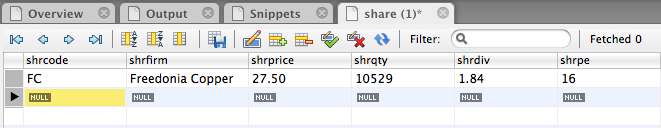
\includegraphics{Figures/Chapter 3/wb-input.png}

\begin{quote}
❓\emph{Skill builder} Create a relational database for the ship entity you modeled previously. Insert some rows.
\end{quote}

\hypertarget{querying-a-database}{%
\subsubsection*{Querying a database}\label{querying-a-database}}
\addcontentsline{toc}{subsubsection}{Querying a database}

The objective of developing a database is to make it easier to use the stored data to solve problems. Typically, a manager raises a question (e.g., How many shares have a PE ratio greater than 12?). A question or request for information, usually called a query, is then translated into a specific data manipulation or query language. The most widely used query language for relational databases is SQL. After the query has been executed, the resulting data are displayed. In the case of a relational database, the answer to a query is always a table.

There is also a query language called relational algebra, which describes a set of operations on tables. Sometimes it is useful to think of queries in terms of these operations. Where appropriate, we will introduce the corresponding relational algebra operation.

Generally we use a four-phase format for describing queries:

\begin{enumerate}
\def\labelenumi{\arabic{enumi}.}
\item
  A brief explanation of the query's purpose
\item
  The query italics, prefixed by •, and some phrasing you might expect from a manager
\item
  The SQL version of the query
\item
  The results of the query.
\end{enumerate}

\hypertarget{displaying-an-entire-table}{%
\paragraph*{Displaying an entire table}\label{displaying-an-entire-table}}
\addcontentsline{toc}{paragraph}{Displaying an entire table}

All the data in a table can be displayed using the SELECT statement. In SQL, the all part is indicated by an asterisk (*).

List all data in the share table.

\begin{Shaded}
\begin{Highlighting}[]
\KeywordTok{SELECT} \OperatorTok{*} \KeywordTok{FROM} \KeywordTok{share}\NormalTok{;}
\end{Highlighting}
\end{Shaded}

\begin{table}

\caption{\label{tab:unnamed-chunk-6}Displaying records 1 - 10}
\centering
\begin{tabular}[t]{l|l|r|r|r|r}
\hline
shrcode & shrfirm & shrprice & shrqty & shrdiv & shrpe\\
\hline
AR & Abyssinian Ruby & 31.82 & 22010 & 1.32 & 13\\
\hline
BE & Burmese Elephant & 0.07 & 154713 & 0.01 & 3\\
\hline
BS & Bolivian Sheep & 12.75 & 231678 & 1.78 & 11\\
\hline
CS & Canadian Sugar & 52.78 & 4716 & 2.50 & 15\\
\hline
FC & Freedonia Copper & 27.50 & 10529 & 1.84 & 16\\
\hline
ILZ & Indian Lead \& Zinc & 37.75 & 6390 & 3.00 & 12\\
\hline
NG & Nigerian Geese & 35.00 & 12323 & 1.68 & 10\\
\hline
PT & Patagonian Tea & 55.25 & 12635 & 2.50 & 10\\
\hline
ROF & Royal Ostrich Farms & 33.75 & 1234923 & 3.00 & 6\\
\hline
SLG & Sri Lankan Gold & 50.37 & 32868 & 2.68 & 16\\
\hline
\end{tabular}
\end{table}

\hypertarget{projectchoosing-columns}{%
\paragraph*{Project---choosing columns}\label{projectchoosing-columns}}
\addcontentsline{toc}{paragraph}{Project---choosing columns}

The relational algebra operation \textbf{project} creates a new table from the columns of an existing table. Project takes a vertical slice through a table by selecting all the values in specified columns. The projection of \texttt{share} on columns \texttt{shrfirm} and \texttt{shrpe} produces a new table with 10 rows and 2 columns. The SQL syntax for the project operation simply lists the columns to be displayed.

\emph{Report a firm's name and price-earnings ratio.}

\begin{Shaded}
\begin{Highlighting}[]
\KeywordTok{SELECT}\NormalTok{ shrfirm, shrpe }\KeywordTok{FROM} \KeywordTok{share}\NormalTok{;}
\end{Highlighting}
\end{Shaded}

\begin{table}

\caption{\label{tab:unnamed-chunk-7}Displaying records 1 - 10}
\centering
\begin{tabular}[t]{l|r}
\hline
shrfirm & shrpe\\
\hline
Abyssinian Ruby & 13\\
\hline
Burmese Elephant & 3\\
\hline
Bolivian Sheep & 11\\
\hline
Canadian Sugar & 15\\
\hline
Freedonia Copper & 16\\
\hline
Indian Lead \& Zinc & 12\\
\hline
Nigerian Geese & 10\\
\hline
Patagonian Tea & 10\\
\hline
Royal Ostrich Farms & 6\\
\hline
Sri Lankan Gold & 16\\
\hline
\end{tabular}
\end{table}

\hypertarget{restrictchoosing-rows}{%
\paragraph*{Restrict---choosing rows}\label{restrictchoosing-rows}}
\addcontentsline{toc}{paragraph}{Restrict---choosing rows}

The relational algebra operation \textbf{restrict} creates a new table from the rows of an existing table. The operation restricts the new table to those rows that satisfy a specified condition. Restrict takes all columns of an existing table but only those rows that meet the specified condition. The restriction of \texttt{share} to those rows where the PE ratio is less than 12 will give a new table with five rows and six columns. These rows are shaded.

\emph{Restriction of share}

Restrict is implemented in SQL using the WHERE clause to specify the condition on which rows are restricted.

\emph{Get all firms with a price-earnings ratio less than 12.}

\begin{Shaded}
\begin{Highlighting}[]
\KeywordTok{SELECT} \OperatorTok{*} \KeywordTok{FROM} \KeywordTok{share} \KeywordTok{WHERE}\NormalTok{ shrpe }\OperatorTok{\textless{}} \DecValTok{12}\NormalTok{;}
\end{Highlighting}
\end{Shaded}

\begin{table}

\caption{\label{tab:unnamed-chunk-8}5 records}
\centering
\begin{tabular}[t]{l|l|r|r|r|r}
\hline
shrcode & shrfirm & shrprice & shrqty & shrdiv & shrpe\\
\hline
BE & Burmese Elephant & 0.07 & 154713 & 0.01 & 3\\
\hline
BS & Bolivian Sheep & 12.75 & 231678 & 1.78 & 11\\
\hline
NG & Nigerian Geese & 35.00 & 12323 & 1.68 & 10\\
\hline
PT & Patagonian Tea & 55.25 & 12635 & 2.50 & 10\\
\hline
ROF & Royal Ostrich Farms & 33.75 & 1234923 & 3.00 & 6\\
\hline
\end{tabular}
\end{table}

In this example, we have a less than condition for the WHERE clause. All permissible comparison operators are listed below.

\begin{longtable}[]{@{}ll@{}}
\toprule
Comparison operator & Meaning \\
\midrule
\endhead
= & Equal to \\
\textless{} & Less than \\
\textless= & Less than orequal to \\
\textgreater{} & Greater than \\
\textgreater= & Greater than or equal to \\
\textless\textgreater{} & Not equal to \\
\bottomrule
\end{longtable}

In addition to the comparison operators, the BETWEEN construct is available.

a BETWEEN x AND y is equivalent to a \textgreater= x AND a \textless= y

\hypertarget{combining-project-and-restrictchoosing-rows-and-columns}{%
\paragraph*{Combining project and restrict---choosing rows and columns}\label{combining-project-and-restrictchoosing-rows-and-columns}}
\addcontentsline{toc}{paragraph}{Combining project and restrict---choosing rows and columns}

SQL permits project and restrict to be combined. A single SQL SELECT statement can specify which columns to project and which rows to restrict.

\emph{List the name, price, quantity, and dividend of each firm where the share holding is at least 100,000.}

\begin{Shaded}
\begin{Highlighting}[]
\KeywordTok{SELECT}\NormalTok{ shrfirm, shrprice, shrqty, shrdiv }\KeywordTok{FROM} \KeywordTok{share}
  \KeywordTok{WHERE}\NormalTok{ shrqty }\OperatorTok{\textgreater{}=} \DecValTok{100000}\NormalTok{;}
\end{Highlighting}
\end{Shaded}

\begin{table}

\caption{\label{tab:unnamed-chunk-9}3 records}
\centering
\begin{tabular}[t]{l|r|r|r}
\hline
shrfirm & shrprice & shrqty & shrdiv\\
\hline
Burmese Elephant & 0.07 & 154713 & 0.01\\
\hline
Bolivian Sheep & 12.75 & 231678 & 1.78\\
\hline
Royal Ostrich Farms & 33.75 & 1234923 & 3.00\\
\hline
\end{tabular}
\end{table}

\hypertarget{more-about-where}{%
\paragraph*{More about WHERE}\label{more-about-where}}
\addcontentsline{toc}{paragraph}{More about WHERE}

The WHERE clause can contain several conditions linked by AND or OR. A clause containing AND means all specified conditions must be true for a row to be selected. In the case of OR, at least one of the conditions must be true for a row to be selected.

\emph{Find all firms where the PE is 12 or higher and the share holding is less than 10,000.}

\begin{Shaded}
\begin{Highlighting}[]
\KeywordTok{SELECT} \OperatorTok{*} \KeywordTok{FROM} \KeywordTok{share}
  \KeywordTok{WHERE}\NormalTok{ shrpe }\OperatorTok{\textgreater{}=} \DecValTok{12} \KeywordTok{AND}\NormalTok{ shrqty }\OperatorTok{\textless{}} \DecValTok{10000}\NormalTok{;}
\end{Highlighting}
\end{Shaded}

\begin{table}

\caption{\label{tab:unnamed-chunk-10}2 records}
\centering
\begin{tabular}[t]{l|l|r|r|r|r}
\hline
shrcode & shrfirm & shrprice & shrqty & shrdiv & shrpe\\
\hline
CS & Canadian Sugar & 52.78 & 4716 & 2.5 & 15\\
\hline
ILZ & Indian Lead \& Zinc & 37.75 & 6390 & 3.0 & 12\\
\hline
\end{tabular}
\end{table}

\hypertarget{the-power-of-the-primary-key}{%
\paragraph*{The power of the primary key}\label{the-power-of-the-primary-key}}
\addcontentsline{toc}{paragraph}{The power of the primary key}

The purpose the primary key is to guarantee that any row in a table can be uniquely addressed. In this example, we use \texttt{shrcode} to return a single row because \texttt{shrcode} is unique for each instance of \texttt{share}. The sought code (AR) must be specified in quotes because \texttt{shrcode} was defined as a character string when the table was created.

\emph{Report firms whose code is AR.}

\begin{Shaded}
\begin{Highlighting}[]
\KeywordTok{SELECT} \OperatorTok{*} \KeywordTok{FROM} \KeywordTok{share} \KeywordTok{WHERE}\NormalTok{ shrcode }\OperatorTok{=} \StringTok{\textquotesingle{}AR\textquotesingle{}}\NormalTok{;}
\end{Highlighting}
\end{Shaded}

\begin{table}

\caption{\label{tab:unnamed-chunk-11}1 records}
\centering
\begin{tabular}[t]{l|l|r|r|r|r}
\hline
shrcode & shrfirm & shrprice & shrqty & shrdiv & shrpe\\
\hline
AR & Abyssinian Ruby & 31.82 & 22010 & 1.32 & 13\\
\hline
\end{tabular}
\end{table}

A query based on a non-primary-key column cannot guarantee that a single row is accessed, as the following illustrates.

\emph{Report firms with a dividend of 2.50.}

\begin{Shaded}
\begin{Highlighting}[]
\KeywordTok{SELECT} \OperatorTok{*} \KeywordTok{FROM} \KeywordTok{share} \KeywordTok{WHERE}\NormalTok{ shrdiv }\OperatorTok{=} \FloatTok{2.5}\NormalTok{;}
\end{Highlighting}
\end{Shaded}

\begin{table}

\caption{\label{tab:unnamed-chunk-12}2 records}
\centering
\begin{tabular}[t]{l|l|r|r|r|r}
\hline
shrcode & shrfirm & shrprice & shrqty & shrdiv & shrpe\\
\hline
CS & Canadian Sugar & 52.78 & 4716 & 2.5 & 15\\
\hline
PT & Patagonian Tea & 55.25 & 12635 & 2.5 & 10\\
\hline
\end{tabular}
\end{table}

\hypertarget{the-in-crowd}{%
\paragraph*{The IN crowd}\label{the-in-crowd}}
\addcontentsline{toc}{paragraph}{The IN crowd}

The keyword IN is used with a list to specify a set of values. IN is always paired with a column name. All rows for which a value in the specified column has a match in the list are selected. It is a simpler way of writing a series of OR statements.

\emph{Report data on firms with codes of FC, AR, or SLG.}

\begin{Shaded}
\begin{Highlighting}[]
\KeywordTok{SELECT} \OperatorTok{*} \KeywordTok{FROM} \KeywordTok{share} \KeywordTok{WHERE}\NormalTok{ shrcode }\KeywordTok{IN}\NormalTok{ (}\StringTok{\textquotesingle{}FC\textquotesingle{}}\NormalTok{,}\StringTok{\textquotesingle{}AR\textquotesingle{}}\NormalTok{,}\StringTok{\textquotesingle{}SLG\textquotesingle{}}\NormalTok{);}
\end{Highlighting}
\end{Shaded}

The foregoing query could have also been written as

\begin{Shaded}
\begin{Highlighting}[]
\KeywordTok{SELECT} \OperatorTok{*} \KeywordTok{FROM} \KeywordTok{share}
  \KeywordTok{WHERE}\NormalTok{ shrcode }\OperatorTok{=} \StringTok{\textquotesingle{}FC\textquotesingle{}} \KeywordTok{or}\NormalTok{ shrcode }\OperatorTok{=} \StringTok{\textquotesingle{}AR\textquotesingle{}} \KeywordTok{or}\NormalTok{ shrcode }\OperatorTok{=} \StringTok{\textquotesingle{}SLG\textquotesingle{}}\NormalTok{;}
\end{Highlighting}
\end{Shaded}

\begin{table}

\caption{\label{tab:unnamed-chunk-14}3 records}
\centering
\begin{tabular}[t]{l|l|r|r|r|r}
\hline
shrcode & shrfirm & shrprice & shrqty & shrdiv & shrpe\\
\hline
AR & Abyssinian Ruby & 31.82 & 22010 & 1.32 & 13\\
\hline
FC & Freedonia Copper & 27.50 & 10529 & 1.84 & 16\\
\hline
SLG & Sri Lankan Gold & 50.37 & 32868 & 2.68 & 16\\
\hline
\end{tabular}
\end{table}

\hypertarget{the-not-in-crowd}{%
\paragraph*{The NOT IN crowd}\label{the-not-in-crowd}}
\addcontentsline{toc}{paragraph}{The NOT IN crowd}

A NOT IN list is used to report instances that do not match any of the values.

\emph{Report all firms other than those with the code CS or PT.}

\begin{Shaded}
\begin{Highlighting}[]
\KeywordTok{SELECT} \OperatorTok{*} \KeywordTok{FROM} \KeywordTok{share} \KeywordTok{WHERE}\NormalTok{ shrcode }\KeywordTok{NOT} \KeywordTok{IN}\NormalTok{ (}\StringTok{\textquotesingle{}CS\textquotesingle{}}\NormalTok{,}\StringTok{\textquotesingle{}PT\textquotesingle{}}\NormalTok{);}
\end{Highlighting}
\end{Shaded}

is equivalent to

\begin{Shaded}
\begin{Highlighting}[]
\KeywordTok{SELECT} \OperatorTok{*} \KeywordTok{FROM} \KeywordTok{share} \KeywordTok{WHERE}\NormalTok{ shrcode }\OperatorTok{\textless{}\textgreater{}} \StringTok{\textquotesingle{}CS\textquotesingle{}} \KeywordTok{AND}\NormalTok{ shrcode }\OperatorTok{\textless{}\textgreater{}} \StringTok{\textquotesingle{}PT\textquotesingle{}}\NormalTok{;}
\end{Highlighting}
\end{Shaded}

\begin{table}

\caption{\label{tab:unnamed-chunk-16}8 records}
\centering
\begin{tabular}[t]{l|l|r|r|r|r}
\hline
shrcode & shrfirm & shrprice & shrqty & shrdiv & shrpe\\
\hline
AR & Abyssinian Ruby & 31.82 & 22010 & 1.32 & 13\\
\hline
BE & Burmese Elephant & 0.07 & 154713 & 0.01 & 3\\
\hline
BS & Bolivian Sheep & 12.75 & 231678 & 1.78 & 11\\
\hline
FC & Freedonia Copper & 27.50 & 10529 & 1.84 & 16\\
\hline
ILZ & Indian Lead \& Zinc & 37.75 & 6390 & 3.00 & 12\\
\hline
NG & Nigerian Geese & 35.00 & 12323 & 1.68 & 10\\
\hline
ROF & Royal Ostrich Farms & 33.75 & 1234923 & 3.00 & 6\\
\hline
SLG & Sri Lankan Gold & 50.37 & 32868 & 2.68 & 16\\
\hline
\end{tabular}
\end{table}

\begin{quote}
❓ \emph{Skill Builder}\\
List those shares where the value of the holding exceeds one million.
\end{quote}

\hypertarget{ordering-columns}{%
\paragraph*{Ordering columns}\label{ordering-columns}}
\addcontentsline{toc}{paragraph}{Ordering columns}

The order of reporting columns is identical to their order in the SQL command. For instance, compare the output of the following queries.

\begin{Shaded}
\begin{Highlighting}[]
\KeywordTok{SELECT}\NormalTok{ shrcode, shrfirm }\KeywordTok{FROM} \KeywordTok{share} \KeywordTok{WHERE}\NormalTok{ shrpe }\OperatorTok{=} \DecValTok{10}\NormalTok{;}
\end{Highlighting}
\end{Shaded}

\begin{table}

\caption{\label{tab:unnamed-chunk-17}2 records}
\centering
\begin{tabular}[t]{l|l}
\hline
shrcode & shrfirm\\
\hline
NG & Nigerian Geese\\
\hline
PT & Patagonian Tea\\
\hline
\end{tabular}
\end{table}

\begin{Shaded}
\begin{Highlighting}[]
\KeywordTok{SELECT}\NormalTok{ shrfirm, shrcode }\KeywordTok{FROM} \KeywordTok{share} \KeywordTok{WHERE}\NormalTok{ shrpe }\OperatorTok{=} \DecValTok{10}\NormalTok{;}
\end{Highlighting}
\end{Shaded}

\begin{table}

\caption{\label{tab:unnamed-chunk-18}2 records}
\centering
\begin{tabular}[t]{l|l}
\hline
shrfirm & shrcode\\
\hline
Nigerian Geese & NG\\
\hline
Patagonian Tea & PT\\
\hline
\end{tabular}
\end{table}

\hypertarget{ordering-rows}{%
\paragraph*{Ordering rows}\label{ordering-rows}}
\addcontentsline{toc}{paragraph}{Ordering rows}

People can generally process an ordered (e.g., sorted alphabetically) report faster than an unordered one. In SQL, the ORDER BY clause specifies the row order in a report. The default ordering sequence is ascending (A before B, 1 before 2). Descending is specified by adding DESC after the column name.

\emph{List all firms where PE is at least 10, and order the report in descending PE. Where PE ratios are identical, list firms in alphabetical order.}

\begin{Shaded}
\begin{Highlighting}[]
\KeywordTok{SELECT} \OperatorTok{*} \KeywordTok{FROM} \KeywordTok{share} \KeywordTok{WHERE}\NormalTok{ shrpe }\OperatorTok{\textgreater{}=} \DecValTok{10}
  \KeywordTok{ORDER} \KeywordTok{BY}\NormalTok{ shrpe }\KeywordTok{DESC}\NormalTok{, shrfirm;}
\end{Highlighting}
\end{Shaded}

\begin{table}

\caption{\label{tab:unnamed-chunk-19}8 records}
\centering
\begin{tabular}[t]{l|l|r|r|r|r}
\hline
shrcode & shrfirm & shrprice & shrqty & shrdiv & shrpe\\
\hline
FC & Freedonia Copper & 27.50 & 10529 & 1.84 & 16\\
\hline
SLG & Sri Lankan Gold & 50.37 & 32868 & 2.68 & 16\\
\hline
CS & Canadian Sugar & 52.78 & 4716 & 2.50 & 15\\
\hline
AR & Abyssinian Ruby & 31.82 & 22010 & 1.32 & 13\\
\hline
ILZ & Indian Lead \& Zinc & 37.75 & 6390 & 3.00 & 12\\
\hline
BS & Bolivian Sheep & 12.75 & 231678 & 1.78 & 11\\
\hline
NG & Nigerian Geese & 35.00 & 12323 & 1.68 & 10\\
\hline
PT & Patagonian Tea & 55.25 & 12635 & 2.50 & 10\\
\hline
\end{tabular}
\end{table}

\hypertarget{numeric-versus-character-sorting}{%
\paragraph*{Numeric versus character sorting}\label{numeric-versus-character-sorting}}
\addcontentsline{toc}{paragraph}{Numeric versus character sorting}

Numeric data in character fields (e.g., a product code) do not always sort the way you initially expect. The difference arises from the way data are stored:

\begin{itemize}
\item
  Numeric fields are right justified and have leading zeros.
\item
  Character fields are left justified and have trailing spaces.
\end{itemize}

For example, the value 1066 stored as CHAR(4) would be stored as `1066' and the value 45 would be stored as `45'. If the column containing these data is sorted in ascending order, then `1066' precedes ' 45 ' because the leftmost character `1' is less than `4'. You can avoid this problem by always storing numeric values as numeric data types (e.g., integer or decimal) or preceding numeric values with zeros when they are stored as character data. Alternatively, start numbering at 1,000 so that all values are four digits, though the best solution is to store numeric data as numbers rather than characters.

\hypertarget{derived-data}{%
\paragraph*{Derived data}\label{derived-data}}
\addcontentsline{toc}{paragraph}{Derived data}

One of the important principles of database design is to avoid redundancy. One form of redundancy is including a column in a table when these data can be derived from other columns. For example, we do not need a column for yield because it can be calculated by dividing dividend by price and multiplying by 100 to obtain the yield as a percentage. This means that the query language does the calculation when the value is required.

\emph{Get firm name, price, quantity, and firm yield.}

\begin{Shaded}
\begin{Highlighting}[]
\KeywordTok{SELECT}\NormalTok{ shrfirm, shrprice, shrqty, shrdiv}\OperatorTok{/}\NormalTok{shrprice}\OperatorTok{*}\DecValTok{100} \KeywordTok{AS}\NormalTok{ yield }\KeywordTok{FROM} \KeywordTok{share}\NormalTok{;}
\end{Highlighting}
\end{Shaded}

\begin{table}

\caption{\label{tab:unnamed-chunk-20}Displaying records 1 - 10}
\centering
\begin{tabular}[t]{l|r|r|r}
\hline
shrfirm & shrprice & shrqty & yield\\
\hline
Abyssinian Ruby & 31.82 & 22010 & 4.148334\\
\hline
Burmese Elephant & 0.07 & 154713 & 14.285714\\
\hline
Bolivian Sheep & 12.75 & 231678 & 13.960784\\
\hline
Canadian Sugar & 52.78 & 4716 & 4.736643\\
\hline
Freedonia Copper & 27.50 & 10529 & 6.690909\\
\hline
Indian Lead \& Zinc & 37.75 & 6390 & 7.947020\\
\hline
Nigerian Geese & 35.00 & 12323 & 4.800000\\
\hline
Patagonian Tea & 55.25 & 12635 & 4.524887\\
\hline
Royal Ostrich Farms & 33.75 & 1234923 & 8.888889\\
\hline
Sri Lankan Gold & 50.37 & 32868 & 5.320627\\
\hline
\end{tabular}
\end{table}

You can give the results of the calculation a column name. In this case, a good choice is \texttt{yield}. Note the use of AS to indicate the name of the column in which the results of the calculation are displayed.

In the preceding query, the keyword AS is introduced to specify an alias, or temporary name. The statement specifies that the result of the calculation is to be reported under the column heading yield. You can rename any column or specify a name for the results of an expression using an alias.

\hypertarget{aggregate-functions}{%
\paragraph*{Aggregate functions}\label{aggregate-functions}}
\addcontentsline{toc}{paragraph}{Aggregate functions}

SQL has built-in functions to enhance its retrieval power and handle many common aggregation queries, such as computing the total value of a column. Four of these functions (AVG, SUM, MIN, and MAX) work very similarly. COUNT is a little different.

\hypertarget{count}{%
\subparagraph*{COUNT}\label{count}}
\addcontentsline{toc}{subparagraph}{COUNT}

COUNT computes the number of rows in a table. Use COUNT(*) to count all rows irrespective of their content (i.e., null or not null), and use COUNT(\texttt{columnname}) to count rows without a null value for \texttt{columname}. Count can be used with a WHERE clause to specify a condition.

\emph{How many firms are there in the portfolio?}

\begin{Shaded}
\begin{Highlighting}[]
\KeywordTok{SELECT} \FunctionTok{COUNT}\NormalTok{(shrcode) }\KeywordTok{AS}\NormalTok{ investments }\KeywordTok{FROM} \KeywordTok{share}\NormalTok{;}
\end{Highlighting}
\end{Shaded}

\begin{table}

\caption{\label{tab:unnamed-chunk-21}1 records}
\centering
\begin{tabular}[t]{r}
\hline
investments\\
\hline
10\\
\hline
\end{tabular}
\end{table}

\emph{How many firms have a holding greater than 50,000?}

\begin{Shaded}
\begin{Highlighting}[]
\KeywordTok{SELECT} \FunctionTok{COUNT}\NormalTok{(shrfirm) }\KeywordTok{AS}\NormalTok{ bigholdings }\KeywordTok{FROM} \KeywordTok{share} \KeywordTok{WHERE}\NormalTok{ shrqty }\OperatorTok{\textgreater{}} \DecValTok{50000}\NormalTok{;}
\end{Highlighting}
\end{Shaded}

\begin{table}

\caption{\label{tab:unnamed-chunk-22}1 records}
\centering
\begin{tabular}[t]{r}
\hline
bigholdings\\
\hline
3\\
\hline
\end{tabular}
\end{table}

\hypertarget{avgaveraging}{%
\subparagraph*{AVG---averaging}\label{avgaveraging}}
\addcontentsline{toc}{subparagraph}{AVG---averaging}

AVG computes the average of the values in a column of numeric data. Null values in the column are not included in the calculation.

\emph{Find the average dividend.}

\begin{Shaded}
\begin{Highlighting}[]
\KeywordTok{SELECT} \FunctionTok{AVG}\NormalTok{(shrdiv) }\KeywordTok{AS}\NormalTok{ avgdiv }\KeywordTok{FROM} \KeywordTok{share}\NormalTok{;}
\end{Highlighting}
\end{Shaded}

\begin{table}

\caption{\label{tab:unnamed-chunk-23}1 records}
\centering
\begin{tabular}[t]{r}
\hline
avgdiv\\
\hline
2.031\\
\hline
\end{tabular}
\end{table}

\emph{What is the average yield for the portfolio?}

\begin{Shaded}
\begin{Highlighting}[]
\KeywordTok{SELECT} \FunctionTok{AVG}\NormalTok{(shrdiv}\OperatorTok{/}\NormalTok{shrprice}\OperatorTok{*}\DecValTok{100}\NormalTok{) }\KeywordTok{AS}\NormalTok{ avgyield }\KeywordTok{FROM} \KeywordTok{share}\NormalTok{;}
\end{Highlighting}
\end{Shaded}

\begin{table}

\caption{\label{tab:unnamed-chunk-24}1 records}
\centering
\begin{tabular}[t]{r}
\hline
avgyield\\
\hline
7.530381\\
\hline
\end{tabular}
\end{table}

\hypertarget{sum-min-and-max}{%
\subparagraph*{SUM, MIN, and MAX}\label{sum-min-and-max}}
\addcontentsline{toc}{subparagraph}{SUM, MIN, and MAX}

SUM, MIN, and MAX differ in the statistic they calculate but are used similarly to AVG. As with AVG, null values in a column are not included in the calculation. SUM computes the sum of a column of values. MIN finds the smallest value in a column; MAX finds the largest.

\hypertarget{subqueries}{%
\paragraph*{Subqueries}\label{subqueries}}
\addcontentsline{toc}{paragraph}{Subqueries}

Sometimes we need the answer to another query before we can write the query of ultimate interest. For example, to list all shares with a PE ratio greater than the portfolio average, you first must find the average PE ratio for the portfolio. You could do the query in two stages:

\begin{Shaded}
\begin{Highlighting}[]
\KeywordTok{SELECT} \FunctionTok{AVG}\NormalTok{(shrpe) }\KeywordTok{FROM} \KeywordTok{share}\NormalTok{;}
\end{Highlighting}
\end{Shaded}

and

\begin{Shaded}
\begin{Highlighting}[]
\KeywordTok{SELECT}\NormalTok{ shrfirm, shrpe }\KeywordTok{FROM} \KeywordTok{share} \KeywordTok{WHERE}\NormalTok{ shrpe }\OperatorTok{\textgreater{}}\NormalTok{ x;}
\end{Highlighting}
\end{Shaded}

where x is the value returned from the first query.

Unfortunately, the two-stage method introduces the possibility of errors. You might forget the value returned by the first query or enter it incorrectly. It also takes longer to get the results of the query. We can solve these problems by using parentheses to indicate the first query is nested within the second one. As a result, the value returned by the inner or nested subquery, the one in parentheses, is used in the outer query. In the following example, the nested query returns 11.20, which is then automatically substituted in the outer query.

\emph{Report all firms with a PE ratio greater than the average for the portfolio.}

\begin{Shaded}
\begin{Highlighting}[]
\KeywordTok{SELECT}\NormalTok{ shrfirm, shrpe }\KeywordTok{FROM} \KeywordTok{share}
  \KeywordTok{WHERE}\NormalTok{ shrpe }\OperatorTok{\textgreater{}}\NormalTok{ (}\KeywordTok{SELECT} \FunctionTok{AVG}\NormalTok{(shrpe) }\KeywordTok{FROM} \KeywordTok{share}\NormalTok{);}
\end{Highlighting}
\end{Shaded}

\begin{table}

\caption{\label{tab:unnamed-chunk-27}5 records}
\centering
\begin{tabular}[t]{l|r}
\hline
shrfirm & shrpe\\
\hline
Abyssinian Ruby & 13\\
\hline
Canadian Sugar & 15\\
\hline
Freedonia Copper & 16\\
\hline
Indian Lead \& Zinc & 12\\
\hline
Sri Lankan Gold & 16\\
\hline
\end{tabular}
\end{table}

\begin{quote}
⚠️ The preceding query is often mistakenly written as\\
SELECT shrfirm, shrpe from share WHERE shrpe \textgreater{} avg(shrpe);
\end{quote}

\begin{quote}
❓\emph{Skill builder}\\
Find the name of the firm for which the value of the holding is greatest.
\end{quote}

\hypertarget{regular-expressionpattern-matching}{%
\paragraph*{Regular expression---pattern matching}\label{regular-expressionpattern-matching}}
\addcontentsline{toc}{paragraph}{Regular expression---pattern matching}

Regular expression is a concise and powerful method for searching for a specified pattern in a nominated column. Regular expression processing is supported by languages such as Java, R, and PHP. In this chapter, we introduce a few typical regular expressions and will continue developing your knowledge of this feature in the next chapter.

\hypertarget{search-for-a-string}{%
\subparagraph*{Search for a string}\label{search-for-a-string}}
\addcontentsline{toc}{subparagraph}{Search for a string}

\emph{List all firms containing `Ruby' in their name.}

\begin{Shaded}
\begin{Highlighting}[]
\KeywordTok{SELECT}\NormalTok{ shrfirm }\KeywordTok{FROM} \KeywordTok{share} \KeywordTok{WHERE}\NormalTok{ shrfirm REGEXP }\StringTok{\textquotesingle{}Ruby\textquotesingle{}}\NormalTok{;}
\end{Highlighting}
\end{Shaded}

\begin{table}

\caption{\label{tab:unnamed-chunk-28}1 records}
\centering
\begin{tabular}[t]{l}
\hline
shrfirm\\
\hline
Abyssinian Ruby\\
\hline
\end{tabular}
\end{table}

\hypertarget{search-for-alternative-strings}{%
\subparagraph*{Search for alternative strings}\label{search-for-alternative-strings}}
\addcontentsline{toc}{subparagraph}{Search for alternative strings}

In some situations you want to find columns that contain more than one string. In this case, we use the alternation symbol `\textbar{}' to indicate the alternatives being sought. For example, a\textbar b finds `a' or `b'.

\emph{List the firms containing gold or zinc in their name, irrespective of case.}

\begin{Shaded}
\begin{Highlighting}[]
\KeywordTok{SELECT}\NormalTok{ shrfirm }\KeywordTok{FROM} \KeywordTok{share} \KeywordTok{WHERE}\NormalTok{ shrfirm REGEXP }\StringTok{\textquotesingle{}gold|zinc|Gold|Zinc\textquotesingle{}}\NormalTok{;}
\end{Highlighting}
\end{Shaded}

\begin{table}

\caption{\label{tab:unnamed-chunk-29}2 records}
\centering
\begin{tabular}[t]{l}
\hline
shrfirm\\
\hline
Indian Lead \& Zinc\\
\hline
Sri Lankan Gold\\
\hline
\end{tabular}
\end{table}

\hypertarget{search-for-a-beginning-string}{%
\subparagraph*{Search for a beginning string}\label{search-for-a-beginning-string}}
\addcontentsline{toc}{subparagraph}{Search for a beginning string}

If you are interested in finding a value in a column that starts with a particular character string, then use \^{} to indicate this option.

\emph{List the firms whose name begins with Sri.}

\begin{Shaded}
\begin{Highlighting}[]
\KeywordTok{SELECT}\NormalTok{ shrfirm }\KeywordTok{FROM} \KeywordTok{share} \KeywordTok{WHERE}\NormalTok{ shrfirm REGEXP }\StringTok{\textquotesingle{}\^{}Sri\textquotesingle{}}\NormalTok{;}
\end{Highlighting}
\end{Shaded}

\begin{table}

\caption{\label{tab:unnamed-chunk-30}1 records}
\centering
\begin{tabular}[t]{l}
\hline
shrfirm\\
\hline
Sri Lankan Gold\\
\hline
\end{tabular}
\end{table}

\hypertarget{search-for-an-ending-string}{%
\subparagraph*{Search for an ending string}\label{search-for-an-ending-string}}
\addcontentsline{toc}{subparagraph}{Search for an ending string}

If you are interested in finding if a value in a column ends with a particular character string, then use \$ to indicate this option.

\emph{List the firms whose name ends with Geese.}

\begin{Shaded}
\begin{Highlighting}[]
\KeywordTok{SELECT}\NormalTok{ shrfirm }\KeywordTok{FROM} \KeywordTok{share} \KeywordTok{WHERE}\NormalTok{ shrfirm REGEXP }\StringTok{\textquotesingle{}Geese$\textquotesingle{}}\NormalTok{;}
\end{Highlighting}
\end{Shaded}

\begin{table}

\caption{\label{tab:unnamed-chunk-31}1 records}
\centering
\begin{tabular}[t]{l}
\hline
shrfirm\\
\hline
Nigerian Geese\\
\hline
\end{tabular}
\end{table}

\begin{quote}
❓\emph{Skill builder}
\end{quote}

\begin{quote}
List the firms containing ``ian'' in their name.
\end{quote}

\hypertarget{distincteliminating-duplicate-rows}{%
\paragraph*{DISTINCT---eliminating duplicate rows}\label{distincteliminating-duplicate-rows}}
\addcontentsline{toc}{paragraph}{DISTINCT---eliminating duplicate rows}

The DISTINCT clause is used to eliminate duplicate rows. It can be used with column functions or before a column name. When used with a column function, it ignores duplicate values.

\emph{Report the different values of the PE ratio.}

\begin{Shaded}
\begin{Highlighting}[]
\KeywordTok{SELECT} \KeywordTok{DISTINCT}\NormalTok{ shrpe }\KeywordTok{FROM} \KeywordTok{share}\NormalTok{;}
\end{Highlighting}
\end{Shaded}

\begin{table}

\caption{\label{tab:unnamed-chunk-32}8 records}
\centering
\begin{tabular}[t]{r}
\hline
shrpe\\
\hline
13\\
\hline
3\\
\hline
11\\
\hline
15\\
\hline
16\\
\hline
12\\
\hline
10\\
\hline
6\\
\hline
\end{tabular}
\end{table}

\emph{Find the number of different PE ratios.}

\begin{Shaded}
\begin{Highlighting}[]
\KeywordTok{SELECT} \FunctionTok{COUNT}\NormalTok{(}\KeywordTok{DISTINCT}\NormalTok{ shrpe) }\KeywordTok{as} \StringTok{\textquotesingle{}Different PEs\textquotesingle{}} \KeywordTok{FROM} \KeywordTok{share}\NormalTok{;}
\end{Highlighting}
\end{Shaded}

\begin{table}

\caption{\label{tab:unnamed-chunk-33}1 records}
\centering
\begin{tabular}[t]{r}
\hline
Different PEs\\
\hline
8\\
\hline
\end{tabular}
\end{table}

When used before a column name, DISTINCT prevents the selection of duplicate rows. Notice a slightly different use of the keyword AS. In this case, because the alias includes a space, the entire alias is enclosed in straight quotes.

\hypertarget{delete}{%
\paragraph*{DELETE}\label{delete}}
\addcontentsline{toc}{paragraph}{DELETE}

Rows in a table can be deleted using the DELETE clause in an SQL statement. DELETE is typically used with a WHERE clause to specify the rows to be deleted. If there is no WHERE clause, all rows are deleted.

\emph{Erase the data for Burmese Elephant. All the shares have been sold.}

\begin{Shaded}
\begin{Highlighting}[]
\KeywordTok{DELETE} \KeywordTok{FROM} \KeywordTok{share} \KeywordTok{WHERE}\NormalTok{ shrfirm }\OperatorTok{=} \StringTok{\textquotesingle{}Burmese Elephant\textquotesingle{}}\NormalTok{;}
\end{Highlighting}
\end{Shaded}

In the preceding statement, \texttt{shrfirm} is used to indicate the row to be deleted.

\hypertarget{update}{%
\paragraph*{UPDATE}\label{update}}
\addcontentsline{toc}{paragraph}{UPDATE}

Rows can be modified using SQL's UPDATE clause, which is used with a WHERE clause to specify the rows to be updated.

\emph{Change the share price of FC to 31.50.}

\begin{Shaded}
\begin{Highlighting}[]
\KeywordTok{UPDATE} \KeywordTok{share} \KeywordTok{SET}\NormalTok{ shrprice }\OperatorTok{=} \FloatTok{31.50} \KeywordTok{WHERE}\NormalTok{ shrcode }\OperatorTok{=} \StringTok{\textquotesingle{}FC\textquotesingle{}}\NormalTok{;}
\end{Highlighting}
\end{Shaded}

\emph{Increase the total number of shares for Nigerian Geese by 10\% because of the recent bonus issue.}

\begin{Shaded}
\begin{Highlighting}[]
\KeywordTok{UPDATE} \KeywordTok{share} \KeywordTok{SET}\NormalTok{ shrqty }\OperatorTok{=}\NormalTok{ shrqty}\OperatorTok{*}\FloatTok{1.1} \KeywordTok{WHERE}\NormalTok{ shrfirm }\OperatorTok{=} \StringTok{\textquotesingle{}Nigerian Geese\textquotesingle{}}\NormalTok{;}
\end{Highlighting}
\end{Shaded}

\hypertarget{quotes}{%
\paragraph*{Quotes}\label{quotes}}
\addcontentsline{toc}{paragraph}{Quotes}

There are three types of quotes that you can typically use with SQL. Double and single quotes are equivalent and can be used interchangeably. Note that single and double quotes must be straight rather than curly, and the back quote is to the left of the 1 key.

\begin{longtable}[]{@{}ll@{}}
\toprule
Type of quote & Representation \\
\midrule
\endhead
Single & \textbf{'} \\
Double & \textbf{"} \\
Back & \textbf{`} \\
\bottomrule
\end{longtable}

The following SQL illustrates the use of three types of quotes to find a person with a last name of O'Hara and where the column names are \texttt{person\ first} and \texttt{person\ last}.

\begin{Shaded}
\begin{Highlighting}[]
\KeywordTok{SELECT}\NormalTok{ \textasciigrave{}person first\textasciigrave{} }\KeywordTok{FROM}\NormalTok{ person }\KeywordTok{WHERE}\NormalTok{ \textasciigrave{}person last\textasciigrave{} }\OperatorTok{=} \OtherTok{"O\textquotesingle{}Hara"}\NormalTok{;}
\end{Highlighting}
\end{Shaded}

\begin{table}

\caption{\label{tab:unnamed-chunk-37}1 records}
\centering
\begin{tabular}[t]{l}
\hline
person first\\
\hline
Sheila\\
\hline
\end{tabular}
\end{table}

\hypertarget{debriefing}{%
\paragraph*{Debriefing}\label{debriefing}}
\addcontentsline{toc}{paragraph}{Debriefing}

Now that you have learned how to model a single entity, create a table, and specify queries, you are on the way to mastering the fundamental skills of database design, implementation, and use. Remember, planning occurs before action. A data model is a plan for a database. The action side of a database is inserting rows and running queries.

\hypertarget{summary-2}{%
\subsection*{Summary}\label{summary-2}}
\addcontentsline{toc}{subsection}{Summary}

The relational database model is an effective means of representing real-world relationships. Data modeling is used to determine what data must be stored and how data are related. An entity is something in the environment. An entity has attributes, which describe it, and an identifier, which uniquely distinguishes an instance of an entity. Every entity must have a unique identifier. A relational database consists of tables with rows and columns. A data model is readily translated into a relational database. The SQL statement CREATE is used to define a table. Rows are added to a table using INSERT. In SQL, queries are written using the SELECT statement. Project (choosing columns) and restrict (choosing rows) are common table operations. The WHERE clause is used to specify row selection criteria. WHERE can be combined with IN and NOT IN, which specify values for a single column. The rows of a report are sorted using the ORDER BY clause. Arithmetic expressions can appear in SQL statements, and SQL has built-in functions for common arithmetic operations. A subquery is a query within a query. Regular expressions are used to find string patterns within character strings. Duplicate rows are eliminated with the DISTINCT clause. Rows can be erased using DELETE or modified with UPDATE.

\hypertarget{key-terms-and-concepts}{%
\subsection*{Key terms and concepts}\label{key-terms-and-concepts}}
\addcontentsline{toc}{subsection}{Key terms and concepts}

\begin{longtable}[]{@{}ll@{}}
\toprule
& \\
\midrule
\endhead
Alias & Instance \\
AS & MAX \\
Attribute & MIN \\
AVG & NOT IN \\
Column & ORDER BY \\
COUNT & Primary key \\
CREATE & Project \\
Data modeling & Relational database \\
Data type & Restrict \\
Database & Row \\
DELETE & SELECT \\
DISTINCT & SQL \\
Entity & Subquery \\
Entity integrity rule & SUM \\
Identifier & Table \\
IN & UPDATE \\
INSERT & WHERE \\
\bottomrule
\end{longtable}

\hypertarget{exercises-2}{%
\subsection*{Exercises}\label{exercises-2}}
\addcontentsline{toc}{subsection}{Exercises}

\begin{enumerate}
\def\labelenumi{\arabic{enumi}.}
\item
  Draw data models for the following entities. In each case, make certain that you show the attributes and identifiers. Also, create a relational database and insert some rows for each of the models.

  \begin{enumerate}
  \def\labelenumii{\alph{enumii}.}
  \item
    Aircraft: An aircraft has a manufacturer, model number, call sign (e.g., N123D), payload, and a year of construction. Aircraft are classified as civilian or military.
  \item
    Car: A car has a manufacturer, range name, and style code (e.g., a Honda Accord DX, where Honda is the manufacturer, Accord is the range, and DX is the style). A car also has a vehicle identification code, registration code, and color.
  \item
    Restaurant: A restaurant has an address, seating capacity, phone number, and style of food (e.g., French, Russian, Chinese).
  \item
    Cow: A dairy cow has a name, date of birth, breed (e.g., Holstein), and a numbered plastic ear tag.
  \end{enumerate}
\item
  Do the following queries using SQL:

  \begin{enumerate}
  \def\labelenumii{\alph{enumii}.}
  \item
    List a share's name and its code.
  \item
    List full details for all shares with a price less than \$1.
  \item
    List the names and prices of all shares with a price of at least \$10.
  \item
    Create a report showing firm name, share price, share holding, and total value of shares held. (Value of shares held is price times quantity.)
  \item
    List the names of all shares with a yield exceeding 5 percent.
  \item
    Report the total dividend payment of Patagonian Tea. (The total dividend payment is dividend times quantity.)
  \item
    Find all shares where the price is less than 20 times the dividend.
  \item
    Find the share(s) with the minimum yield.
  \item
    Find the total value of all shares with a PE ratio \textgreater{} 10.
  \item
    Find the share(s) with the maximum total dividend payment.
  \item
    Find the value of the holdings in Abyssinian Ruby and Sri Lankan Gold.
  \item
    Find the yield of all firms except Bolivian Sheep and Canadian Sugar.
  \item
    Find the total value of the portfolio.
  \item
    List firm name and value in descending order of value.
  \item
    List shares with a firm name containing ``Gold.''
  \item
    Find shares with a code starting with ``B.''
  \end{enumerate}
\item
  Run the following queries and explain the differences in output. Write each query as a manager might state it.

  \begin{enumerate}
  \def\labelenumii{\alph{enumii}.}
  \item
    SELECT shrfirm FROM share WHERE shrfirm NOT REGEXP `s';
  \item
    SELECT shrfirm FROM share WHERE shrfirm NOT REGEXP `S';
  \item
    SELECT shrfirm FROM share WHERE shrfirm NOT REGEXP `s\textbar S';
  \item
    SELECT shrfirm FROM share WHERE shrfirm NOT REGEXP `\^{}S';
  \item
    SELECT shrfirm FROM share WHERE shrfirm NOT REGEXP `s\$';
  \end{enumerate}
\item
  A weekly newspaper, sold at supermarket checkouts, frequently reports stories of aliens visiting Earth and taking humans on short trips. Sometimes a captured human sees Elvis commanding the spaceship. To keep track of all these reports, the newspaper has created the following data model.
\end{enumerate}

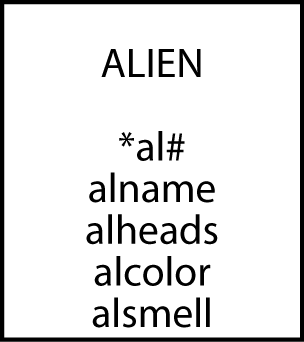
\includegraphics[width=1.58333in,height=\textheight]{Figures/Chapter 3/alien entity.png}

The paper has also supplied some data for the last few sightings and asked you to create the database, add details of these aliens, and answer the following queries:

\begin{verbatim}
a.  What's the average number of heads of an alien?

a.  Which alien has the most heads?

b.  Are there any aliens with a double o in their names?

c.  How many aliens are chartreuse?

d.  Report details of all aliens sorted by smell and color.
\end{verbatim}

\begin{enumerate}
\def\labelenumi{\arabic{enumi}.}
\setcounter{enumi}{4}
\item
  Eduardo, a bibliophile, has a collection of several hundred books. Being a little disorganized, he has his books scattered around his den. They are piled on the floor, some are in bookcases, and others sit on top of his desk. Because he has so many books, he finds it difficult to remember what he has, and sometimes he cannot find the book he wants. Eduardo has a simple personal computer file system that is fine for a single entity or file. He has decided that he would like to list each book by author(s)' name and type of book (e.g., literature, travel, reference). Draw a data model for this problem, create a single entity table, and write some SQL queries.

  \begin{enumerate}
  \def\labelenumii{\alph{enumii}.}
  \item
    How do you identify each instance of a book? (It might help to look at a few books.)
  \item
    How should Eduardo physically organize his books to permit fast retrieval of a particular one?
  \item
    Are there any shortcomings with the data model you have created?
  \end{enumerate}
\item
  What is an identifier? Why does a data model have an identifier?
\item
  What are entities?
\item
  What is the entity integrity rule?
\end{enumerate}

\hypertarget{the-one-to-many-relationship}{%
\section{The One-to-Many Relationship}\label{the-one-to-many-relationship}}

\begin{quote}
\emph{Cow of many---well milked and badly fed.}

Spanish proverb
\end{quote}

\hypertarget{learning-objectives-3}{%
\subsubsection*{Learning Objectives}\label{learning-objectives-3}}
\addcontentsline{toc}{subsubsection}{Learning Objectives}

Students completing this chapter will be able to

\begin{itemize}
\item
  model a one-to-many relationship between two entities;
\item
  define a database with a one-to-many relationship;
\item
  write queries for a database with a one-to-many relationship.
\end{itemize}

\hypertarget{relationships}{%
\subsection*{Relationships}\label{relationships}}
\addcontentsline{toc}{subsection}{Relationships}

Entities are not isolated; they are related to other entities. When we
move beyond the single entity, we need to identify the relationships
between entities to accurately represent the real world. Consider the
case where a person's stocks are listed in different countries. We now
need to introduce an entity called NATION. We now have two entities,
STOCK and NATION. Consider the relationship between them. A NATION can
have many listed stocks. A stock, in this case, is listed in only one
nation. There is a 1:m (one-to-many) relationship between NATION and
STOCK.

A 1:m relationship between two entities is depicted by a line connecting
the two with a crow's foot at the many end of the relationship. The
following figure shows the 1:m relationship between NATION and STOCK.
This can be read as: ``a nation can have many stocks, but a stock belongs
to only one nation.'' The entity NATION is identified by \emph{nation code}
and has attributes \emph{nation name} and \emph{exchange rate}.

\emph{A 1:m relationship between NATION and STOCK}

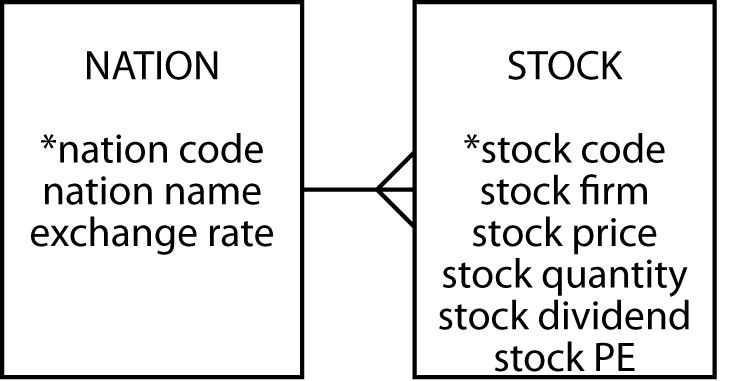
\includegraphics[width=3.91667in,height=\textheight]{Figures/Chapter 4/nation-stock.png}

The 1:m relationship occurs frequently in business situations. Sometimes
it occurs in a tree or hierarchical fashion. Consider a very
hierarchical firm. It has many divisions, but a division belongs to only
one firm. A division has many departments, but a department belongs to
only one division. A department has many sections, but a section belongs
to only one department.

\emph{A series of 1:m relationships}

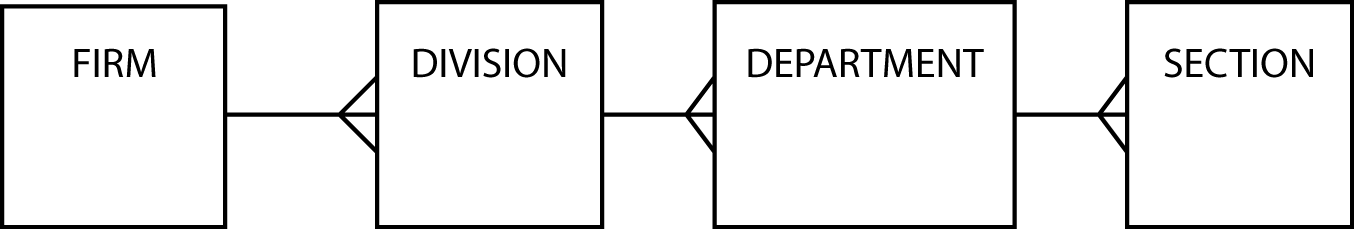
\includegraphics{Figures/Chapter 4/hierarchy.png}

\hypertarget{why-did-we-create-an-additional-entity}{%
\subsubsection*{Why did we create an additional entity?}\label{why-did-we-create-an-additional-entity}}
\addcontentsline{toc}{subsubsection}{Why did we create an additional entity?}

Another approach to adding data about listing nation and exchange rate
is to add two attributes to STOCK: \emph{nation name} and \emph{exchange rate}. At
first glance, this seems a very workable solution; however, this will
introduce considerable redundancy, as the following table illustrates.

\emph{The table stock with additional columns}

\begin{longtable}[]{@{}llllllll@{}}
\toprule
\underline{stkcode} & stkfirm & stkprice & stkqty & stkdiv & stkpe & natname & exchrate \\
\midrule
\endhead
FC & Freedonia Copper & 27.5 & 10529 & 1.84 & 16 & United Kingdom & 1 \\
PT & Patagonian Tea & 55.25 & 12635 & 2.5 & 10 & United Kingdom & 1 \\
AR & Abyssinian Ruby & 31.82 & 22010 & 1.32 & 13 & United Kingdom & 1 \\
SLG & Sri Lankan Gold & 50.37 & 32868 & 2.68 & 16 & United Kingdom & 1 \\
ILZ & Indian Lead \& Zinc & 37.75 & 6390 & 3 & 12 & United Kingdom & 1 \\
BE & Burmese Elephant & 0.07 & 154713 & 0.01 & 3 & United Kingdom & 1 \\
BS & Bolivian Sheep & 12.75 & 231678 & 1.78 & 11 & United Kingdom & 1 \\
NG & Nigerian Geese & 35 & 12323 & 1.68 & 10 & United Kingdom & 1 \\
CS & Canadian Sugar & 52.78 & 4716 & 2.5 & 15 & United Kingdom & 1 \\
ROF & Royal Ostrich Farms & 33.75 & 1234923 & 3 & 6 & United Kingdom & 1 \\
MG & Minnesota Gold & 53.87 & 816122 & 1 & 25 & USA & 0.67 \\
GP & Georgia Peach & 2.35 & 387333 & 0.2 & 5 & USA & 0.67 \\
NE & Narembeen Emu & 12.34 & 45619 & 1 & 8 & Australia & 0.46 \\
QD & Queensland Diamond & 6.73 & 89251 & 0.5 & 7 & Australia & 0.46 \\
IR & Indooroopilly Ruby & 15.92 & 56147 & 0.5 & 20 & Australia & 0.46 \\
BD & Bombay Duck & 25.55 & 167382 & 1 & 12 & India & 0.0228 \\
\bottomrule
\end{longtable}

The exact same nation name and \emph{e}xchange rate data pair occurs 10 times
for stocks listed in the United Kingdom. Redundancy presents problems
when we want to insert, delete, or update data. These problems,
generally known as \textbf{update anomalies}, occur with these three basic
operations.

\hypertarget{insert-anomalies}{%
\paragraph*{Insert anomalies}\label{insert-anomalies}}
\addcontentsline{toc}{paragraph}{Insert anomalies}

We cannot insert a fact about a nation's exchange rate unless we first
buy a stock that is listed in that nation. Consider the case where we
want to keep a record of France's exchange rate and we have no French
stocks. We cannot skirt this problem by putting in a null entry for
stock details because stkcode, the primary key, would be null, and this
is not allowed. If we have a separate table for facts about a nation,
then we can easily add new nations without having to buy stocks. This is
particularly useful when other parts of the organization, say
International Trading, also need access to exchange rates for many
nations.

\hypertarget{delete-anomalies}{%
\paragraph*{Delete anomalies}\label{delete-anomalies}}
\addcontentsline{toc}{paragraph}{Delete anomalies}

If we delete data about a particular stock, we might also lose a fact
about exchange rates. For example, if we delete details of Bombay Duck,
we also erase the Indian exchange rate.

\hypertarget{update-anomalies}{%
\paragraph*{Update anomalies}\label{update-anomalies}}
\addcontentsline{toc}{paragraph}{Update anomalies}

Exchange rates are volatile. Most companies need to update them every
day. What happens when the Australian exchange rate changes? Every row
in stock with nation = `Australia' will have to be updated. In a large
portfolio, many rows will be changed. There is also the danger of
someone forgetting to update all the instances of the nation and
exchange rate pair. As a result, there could be two exchange rates for
the one nation. If exchange rate is stored in nation, however, only one
change is necessary, there is no redundancy, and there is no danger of
inconsistent exchange rates.

\hypertarget{creating-a-database-with-a-1m-relationship}{%
\subsection*{Creating a database with a 1:m relationship}\label{creating-a-database-with-a-1m-relationship}}
\addcontentsline{toc}{subsection}{Creating a database with a 1:m relationship}

As before, each entity becomes a table in a relational database, the
entity name becomes the table name, each attribute becomes a column, and
each identifier becomes a primary key. The 1:m relationship is mapped by
adding a column to the entity at the many end of the relationship. The
additional column contains the identifier of the one end of the
relationship.

Consider the relationship between the entities STOCK and NATION. The
database has two tables: \texttt{stock} and \texttt{nation.} The table stock has an
additional column, natcode, which contains the primary key of nation. If
natcode is not stored in \texttt{stock}, then there is no way of knowing the
identity of the nation where the \texttt{stock} is listed.

\emph{A relational database with tables nation and stock}

\begin{longtable}[]{@{}llll@{}}
\toprule
nation & & & \\
\midrule
\endhead
\underline{natcode} & natname & exchrate & \\
AUS & Australia & 0.46 & \\
IND & India & 0.0228 & \\
UK & United Kingdom & 1 & \\
USA & United States & 0.67 & → \\
\bottomrule
\end{longtable}

\begin{longtable}[]{@{}llllllll@{}}
\toprule
stock & & & & & & & \\
\midrule
\endhead
\underline{stkcode} & stkfirm & stkprice & stkqty & stkdiv & stkpe & \emph{natcode} & \\
FC & Freedonia Copper & 27.5 & 10,529 & 1.84 & 16 & UK & \\
PT & Patagonian Tea & 55.25 & 12,635 & 2.5 & 10 & UK & \\
AR & Abyssinian Ruby & 31.82 & 22,010 & 1.32 & 13 & UK & \\
SLG & Sri Lankan Gold & 50.37 & 32,868 & 2.68 & 16 & UK & \\
ILZ & Indian Lead \& Zinc & 37.75 & 6,390 & 3 & 12 & UK & \\
BE & Burmese Elephant & 0.07 & 154,713 & 0.01 & 3 & UK & \\
BS & Bolivian Sheep & 12.75 & 231,678 & 1.78 & 11 & UK & \\
NG & Nigerian Geese & 35 & 12,323 & 1.68 & 10 & UK & \\
CS & Canadian Sugar & 52.78 & 4,716 & 2.5 & 15 & UK & \\
ROF & Royal Ostrich Farms & 33.75 & 1,234,923 & 3 & 6 & UK & \\
MG & Minnesota Gold & 53.87 & 816,122 & 1 & 25 & USA & ← \\
GP & Georgia Peach & 2.35 & 387,333 & 0.2 & 5 & USA & ← \\
NE & Narembeen Emu & 12.34 & 45,619 & 1 & 8 & AUS & \\
QD & Queensland Diamond & 6.73 & 89,251 & 0.5 & 7 & AUS & \\
IR & Indooroopilly Ruby & 15.92 & 56,147 & 0.5 & 20 & AUS & \\
BD & Bombay Duck & 25.55 & 167,382 & 1 & 12 & IND & \\
\bottomrule
\end{longtable}

Notice that \texttt{natcode} appears in both the \texttt{stock} and \texttt{nation} tables.
In \texttt{nation}, \texttt{natcode} is the primary key; it is unique for each
instance of \texttt{nation.} In table \texttt{stock}, \texttt{natcode} is a \textbf{foreign key}
because it is the primary key of \texttt{nation}, the one end of the 1:m
relationship. The column \texttt{natcode} is a foreign key in \texttt{stock} because
it is a primary key in \texttt{nation}. A matched primary key--foreign key pair
is the method for recording the 1:m relationship between the two tables.
This method of representing a relationship is illustrated using shading
and arrows for the two USA stocks. In the \texttt{stock} table, \texttt{natcode} is
italicized to indicate that it is a foreign key. This method, like
underlining a primary key, is a useful reminder.

Although the same name has been used for the primary key and the foreign
key in this example, it is not mandatory. The two columns can have
different names, and in some cases you are forced to use different
names. When possible, we find it convenient to use identical column
names to help us remember that the tables are related. To distinguish
between columns with identical names, they must by \textbf{qualified} by
prefixing the table name. In this case, use \texttt{nation.natcode} and
\texttt{stock.natcode.} Thus, \texttt{nation.natcode} refers to the \texttt{natcode} column
in the table \texttt{nation.}

Although a nation can have many stocks, it is not mandatory to have any.
That is, in data modeling terminology, many can be zero, one, or more,
but it is mandatory to have a value for \texttt{natcode} in \texttt{nation} for every
value of \texttt{natcode} in \texttt{stock}. This requirement, known as the
\textbf{referential integrity constraint}, maintains the accuracy of a
database. Its application means that every foreign key in a table has an
identical primary key in that same table or another table. In this
example, it means that for every value of \texttt{natcode} in \texttt{stock}, there is
a corresponding entry in \texttt{nation}. As a result, a primary key row must
be created before its corresponding foreign key row. In other words,
details for a \texttt{nation} must be added before any data about its listed
stocks are entered.

Every foreign key must have a matching primary key (referential
integrity rule), and every primary key must be non-null (entity
integrity rule). A foreign key cannot be null when a relationship is
mandatory, as in the case where a stock must belong to a nation. If a
relationship is optional (a person can have a boss), then a foreign key
can be null (i.e., a person is the head of the organization, and thus
has no boss). The ideas of mandatory and optional will be discussed
later in this book.

Why is the foreign key in the table at the ``many'' end of the
relationship? Because each instance of \texttt{stock} is associated with
exactly one instance of \texttt{nation}. The rule is that a \texttt{stock} must be
listed in one, and only one, nation. Thus, the foreign key field is
single-valued when it is at the ``many'' end of a relationship. The
foreign key is not at the ``one'' end of the relationship because each
instance of nation can be associated with more than one instance of
\texttt{stock}, and this implies a multivalued foreign key. The relational
model does not support multivalued fields.

Using SQL, the two tables are defined in a similar manner to the way we
created a single table in Chapter 3. Here are the SQL statements:

\begin{Shaded}
\begin{Highlighting}[]
\KeywordTok{CREATE} \KeywordTok{TABLE}\NormalTok{ nation (}
\NormalTok{  natcode }\DataTypeTok{CHAR}\NormalTok{(}\DecValTok{3}\NormalTok{),}
\NormalTok{  natname }\DataTypeTok{VARCHAR}\NormalTok{(}\DecValTok{20}\NormalTok{),}
\NormalTok{  exchrate }\DataTypeTok{DECIMAL}\NormalTok{(}\DecValTok{9}\NormalTok{,}\DecValTok{5}\NormalTok{),}
  \KeywordTok{PRIMARY} \KeywordTok{KEY}\NormalTok{(natcode));}
\end{Highlighting}
\end{Shaded}

\begin{Shaded}
\begin{Highlighting}[]
\KeywordTok{CREATE} \KeywordTok{TABLE}\NormalTok{ stock (}
\NormalTok{  stkcode }\DataTypeTok{CHAR}\NormalTok{(}\DecValTok{3}\NormalTok{),}
\NormalTok{  stkfirm }\DataTypeTok{VARCHAR}\NormalTok{(}\DecValTok{20}\NormalTok{),}
\NormalTok{  stkprice }\DataTypeTok{DECIMAL}\NormalTok{(}\DecValTok{6}\NormalTok{,}\DecValTok{2}\NormalTok{),}
\NormalTok{  stkqty }\DataTypeTok{DECIMAL}\NormalTok{(}\DecValTok{8}\NormalTok{),}
\NormalTok{  stkdiv }\DataTypeTok{DECIMAL}\NormalTok{(}\DecValTok{5}\NormalTok{,}\DecValTok{2}\NormalTok{),}
\NormalTok{  stkpe }\DataTypeTok{DECIMAL}\NormalTok{(}\DecValTok{5}\NormalTok{),}
\NormalTok{  natcode }\DataTypeTok{CHAR}\NormalTok{(}\DecValTok{3}\NormalTok{),}
  \KeywordTok{PRIMARY} \KeywordTok{KEY}\NormalTok{(stkcode),}
  \KeywordTok{CONSTRAINT}\NormalTok{ fk\_has\_nation }\KeywordTok{FOREIGN} \KeywordTok{KEY}\NormalTok{(natcode)}
  \KeywordTok{REFERENCES}\NormalTok{ nation(natcode) }\KeywordTok{ON} \KeywordTok{DELETE} \KeywordTok{RESTRICT}\NormalTok{);}
\end{Highlighting}
\end{Shaded}

Notice that the definition of \texttt{stock} includes an additional phrase to
specify the foreign key and the referential integrity constraint. The
CONSTRAINT clause defines the column or columns in the table being
created that constitute the foreign key. A referential integrity
constraint can be named, and in this case, the constraint's name is
\texttt{fk\_has\_nation}. The foreign key is the column \texttt{natcode} in STOCK, and
it references the primary key of \texttt{nation}, which is \texttt{natcode}.

The ON DELETE clause specifies what processing should occur if an
attempt is made to delete a row in \texttt{nation} with a primary key that is a
foreign key in \texttt{stock}. In this case, the ON DELETE clause specifies
that it is not permissible (the meaning of RESTRICT) to delete a primary
key row in \texttt{nation} while a corresponding foreign key in \texttt{stock} exists.
In other words, the system will not execute the delete. You must first
delete all corresponding rows in \texttt{stock} before attempting to delete the
row containing the primary key. ON DELETE is the default clause for most
RDBMSs, so we will dispense with specifying it for future foreign key
constraints.

Observe that both the primary and foreign keys are defined as CHAR(3).
The relational model requires that a primary key--foreign key pair have
the same data type and are the same length.

\begin{quote}
❓\emph{Skill builder}

The university architect has asked you to develop a data model to
record details of the campus buildings. A building can have many
rooms, but a room can be in only one building. Buildings have names,
and rooms have a size and purpose (e.g., lecture, laboratory,
seminar). Draw a data model for this situation and create the matching
relational database.
\end{quote}

\hypertarget{mysql-workbench}{%
\subsubsection*{MySQL Workbench}\label{mysql-workbench}}
\addcontentsline{toc}{subsubsection}{MySQL Workbench}

In Workbench, a 1:m relationship is represented in a similar manner to
the method you have just learned. Also, note that the foreign key is
shown in the entity at the many end with a red diamond. We omit the
foreign key when data modeling because it can be inferred. You will
observe some additional symbols on the line between the two entities,
and these will be explained later, but take note of the crow's foot
indicating the 1:m relationship between nation and stock. Because
Workbench can generate automatically the SQL to create the tables,\textsuperscript{11}
we use lowercase table names and abbreviated column names.

\emph{Specifying a 1:m relationship in MySQL Workbench}

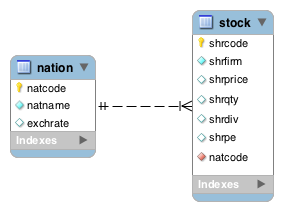
\includegraphics{Figures/Chapter 4/wb-stock-nation.png}

\hypertarget{querying-a-two-table-database}{%
\subsection*{Querying a two-table database}\label{querying-a-two-table-database}}
\addcontentsline{toc}{subsection}{Querying a two-table database}

A two-table database offers the opportunity to learn more SQL and
another relational algebra operation: join.

\hypertarget{join}{%
\subsubsection*{Join}\label{join}}
\addcontentsline{toc}{subsubsection}{Join}

Join creates a new table from two existing tables by matching on a
column common to both tables. Usually, the common column is a primary
key--foreign key pair: The primary key of one table is matched with the
foreign key of another table. Join is frequently used to get the data
for a query into a single row. Consider the tables \texttt{nation} and \texttt{stock}.
If we want to calculate the value---in British pounds---of a stock, we
multiply stock price by stock quantity and then exchange rate. To find
the appropriate exchange rate for a stock, get its \texttt{natcode} from stock
and then find the exchange rate in the matching row in \texttt{nation}, the one
with the same value for \texttt{natcode}. For example, to calculate the value
of Georgia Peach, which has \texttt{natcode} = `US', find the row in \texttt{nation}
that also has \texttt{natcode} = `US'. In this case, the stock's value is
2.35*387333*0.67 = £609,855.81.

Calculation of stock value is very easy once a join is used to get the
three values in one row. The SQL command for joining the two tables is:

\begin{Shaded}
\begin{Highlighting}[]
\KeywordTok{SELECT} \OperatorTok{*} \KeywordTok{FROM}\NormalTok{ stock }\KeywordTok{JOIN}\NormalTok{ nation}
    \KeywordTok{ON}\NormalTok{ stock.natcode }\OperatorTok{=}\NormalTok{ nation.natcode;}
\end{Highlighting}
\end{Shaded}

\begin{table}

\caption{\label{tab:unnamed-chunk-40}Displaying records 1 - 10}
\centering
\begin{tabular}[t]{l|l|r|r|r|r|l|l|l|r}
\hline
stkcode & stkfirm & stkprice & stkqty & stkdiv & stkpe & natcode & natcode & natname & exchrate\\
\hline
IR & Indooroopilly Ruby & 15.92 & 56147 & 0.50 & 20 & AUS & AUS & Australia & 0.4600\\
\hline
NE & Narembeen Emu & 12.34 & 45619 & 1.00 & 8 & AUS & AUS & Australia & 0.4600\\
\hline
QD & Queensland Diamond & 6.73 & 89251 & 0.50 & 7 & AUS & AUS & Australia & 0.4600\\
\hline
BD & Bombay Duck & 25.55 & 167382 & 1.00 & 12 & IND & IND & India & 0.0228\\
\hline
AR & Abyssinian Ruby & 31.82 & 22010 & 1.32 & 13 & UK & UK & United Kingdom & 1.0000\\
\hline
BE & Burmese Elephant & 0.07 & 154713 & 0.01 & 3 & UK & UK & United Kingdom & 1.0000\\
\hline
BS & Bolivian Sheep & 12.75 & 231678 & 1.78 & 11 & UK & UK & United Kingdom & 1.0000\\
\hline
CS & Canadian Sugar & 52.78 & 4716 & 2.50 & 15 & UK & UK & United Kingdom & 1.0000\\
\hline
FC & Freedonia Copper & 27.50 & 10529 & 1.84 & 16 & UK & UK & United Kingdom & 1.0000\\
\hline
ILZ & Indian Lead \& Zinc & 37.75 & 6390 & 3.00 & 12 & UK & UK & United Kingdom & 1.0000\\
\hline
\end{tabular}
\end{table}

\emph{The join of stock and nation}

The columns \texttt{stkprice} and \texttt{stkdiv} record values in the country's
currency. Thus, the price of Bombay Duck is 25.55 Indian rupees. To find
the value in U.K. pounds (GPB), multiply the price by 0.0228, because
one rupee is worth 0.0228 GPB. The value of one share of Bombay Duck in
U.S. dollars (USD) is 25.55*0.0228/0.67 because one USD is worth 0.67
GBP.

There are several things to notice about the SQL command and the result:

\begin{itemize}
\item
  To avoid confusion because \texttt{natcode} is a column name in both stock
  and nation, it needs to be qualified. If \texttt{natcode} is not qualified,
  the system will reject the query because it cannot distinguish
  between the two columns titled \texttt{natcode}.
\item
  The new table has the \texttt{natcode} column replicated. Both are called
  \texttt{natcode}. The naming convention for the replicated column varies
  with the RDBMS. The columns, for example, should be labeled
  \texttt{stock.natcode} and \texttt{nation.natcode}.
\item
  The SQL command specifies the names of the tables to be joined, the
  columns to be used for matching, and the condition for the match
  (equality in this case).
\item
  The number of columns in the new table is the sum of the columns in
  the two tables.
\item
  The stock value calculation is now easily specified in an SQL
  command because all the data are in one row.
\end{itemize}

Remember that during data modeling we created two entities, STOCK and
NATION, and defined the relationship between them. We showed that if the
data were stored in one table, there could be updating problems. Now,
with a join, we have combined these data. So why separate the data only
to put them back together later? There are two reasons. First, we want
to avoid update anomalies. Second, as you will discover, we do not join
the same tables every time.

Join comes in several flavors. The matching condition can be =, \textless\textgreater,
\textless=, \textless, \textgreater=, and \textgreater. This generalized version is called a \textbf{theta
join}. Generally, when people refer to a join, they mean an equijoin,
when the matching condition is equality.

\emph{In an alphabetical list of employees, how many appear before Clare?}

\begin{Shaded}
\begin{Highlighting}[]
\KeywordTok{SELECT} \FunctionTok{count}\NormalTok{(}\OperatorTok{*}\NormalTok{) }\KeywordTok{FROM}\NormalTok{ emp A }\KeywordTok{JOIN}\NormalTok{ emp B}
  \KeywordTok{ON}\NormalTok{ A.empfname }\OperatorTok{\textgreater{}}\NormalTok{ B.empfname}
  \KeywordTok{WHERE}\NormalTok{ A.empfname }\OperatorTok{=} \OtherTok{"Clare"}
\end{Highlighting}
\end{Shaded}

\begin{table}

\caption{\label{tab:unnamed-chunk-41}1 records}
\centering
\begin{tabular}[t]{r}
\hline
count(*)\\
\hline
3\\
\hline
\end{tabular}
\end{table}

A join can be combined with other SQL commands.

\emph{Report the value of each stockholding in UK pounds. Sort the report by
nation and firm.}

\begin{Shaded}
\begin{Highlighting}[]
\KeywordTok{SELECT}\NormalTok{ natname, stkfirm, stkprice, stkqty, exchrate,}
\NormalTok{    stkprice}\OperatorTok{*}\NormalTok{stkqty}\OperatorTok{*}\NormalTok{exchrate }\KeywordTok{as}\NormalTok{ stkvalue}
        \KeywordTok{FROM}\NormalTok{ stock }\KeywordTok{JOIN}\NormalTok{ nation}
            \KeywordTok{ON}\NormalTok{ stock.natcode }\OperatorTok{=}\NormalTok{ nation.natcode}
                \KeywordTok{ORDER} \KeywordTok{BY}\NormalTok{ natname, stkfirm;}
\end{Highlighting}
\end{Shaded}

\begin{table}

\caption{\label{tab:unnamed-chunk-42}Displaying records 1 - 10}
\centering
\begin{tabular}[t]{l|l|r|r|r|r}
\hline
natname & stkfirm & stkprice & stkqty & exchrate & stkvalue\\
\hline
Australia & Indooroopilly Ruby & 15.92 & 56147 & 0.4600 & 411175.71\\
\hline
Australia & Narembeen Emu & 12.34 & 45619 & 0.4600 & 258951.69\\
\hline
Australia & Queensland Diamond & 6.73 & 89251 & 0.4600 & 276303.25\\
\hline
India & Bombay Duck & 25.55 & 167382 & 0.0228 & 97506.71\\
\hline
United Kingdom & Abyssinian Ruby & 31.82 & 22010 & 1.0000 & 700358.20\\
\hline
United Kingdom & Bolivian Sheep & 12.75 & 231678 & 1.0000 & 2953894.50\\
\hline
United Kingdom & Burmese Elephant & 0.07 & 154713 & 1.0000 & 10829.91\\
\hline
United Kingdom & Canadian Sugar & 52.78 & 4716 & 1.0000 & 248910.48\\
\hline
United Kingdom & Freedonia Copper & 27.50 & 10529 & 1.0000 & 289547.50\\
\hline
United Kingdom & Indian Lead \& Zinc & 37.75 & 6390 & 1.0000 & 241222.50\\
\hline
\end{tabular}
\end{table}

\hypertarget{control-break-reporting}{%
\subsubsection*{Control break reporting}\label{control-break-reporting}}
\addcontentsline{toc}{subsubsection}{Control break reporting}

The purpose of a join is to collect the necessary data for a report.
When two tables in a 1:m relationship are joined, the report will
contain repetitive data. If you re-examine the report from the previous
join, you will see that \texttt{nation} and \texttt{exchrate} are often repeated
because the same values apply to many stocks. A more appropriate format
is shown in the following figure, an example of a \textbf{control break
report}.

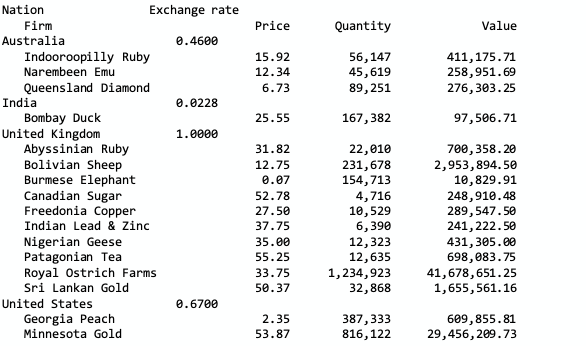
\includegraphics{Figures/Chapter 4/cbr.png}

A control break report recognizes that the values in a particular column
or columns seldom change. In this case, \texttt{natname} and \texttt{exchrate} are
often the same from one row to the next, so it makes sense to report
these data only when they change. The report is also easier to read. The
column \texttt{natname} is known as a \emph{control field}. Notice that there are
four groups of data, because \texttt{natname} has four different values.

Many RDBMS packages have report-writing languages to facilitate creating
a control break report. These languages typically support summary
reporting for each group of rows having the same value for the control
field(s). A table must usually be sorted on the control break field(s)
before the report is created.

\hypertarget{group-byreporting-by-groups}{%
\paragraph*{GROUP BY---reporting by groups}\label{group-byreporting-by-groups}}
\addcontentsline{toc}{paragraph}{GROUP BY---reporting by groups}

The GROUP BY clause is an elementary form of control break reporting. It
permits grouping of rows that have the same value for a specified column
or columns, and it produces one row for each different value of the
grouping column(s).

\emph{Report by nation the total value of stockholdings.}

\begin{Shaded}
\begin{Highlighting}[]
\KeywordTok{SELECT}\NormalTok{ natname, }\FunctionTok{sum}\NormalTok{(stkprice}\OperatorTok{*}\NormalTok{stkqty}\OperatorTok{*}\NormalTok{exchrate) }\KeywordTok{as}\NormalTok{ stkvalue}
    \KeywordTok{FROM}\NormalTok{ stock }\KeywordTok{JOIN}\NormalTok{ nation }\KeywordTok{ON}\NormalTok{ stock.natcode }\OperatorTok{=}\NormalTok{ nation.natcode}
        \KeywordTok{GROUP} \KeywordTok{BY}\NormalTok{ natname;}
\end{Highlighting}
\end{Shaded}

\begin{table}

\caption{\label{tab:unnamed-chunk-43}4 records}
\centering
\begin{tabular}[t]{l|r}
\hline
natname & stkvalue\\
\hline
Australia & 946430.65\\
\hline
India & 97506.71\\
\hline
United Kingdom & 48908364.25\\
\hline
United States & 30066065.54\\
\hline
\end{tabular}
\end{table}

SQL's built-in functions (COUNT, SUM, AVERAGE, MIN, and MAX) can be used
with the GROUP BY clause. They are applied to a group of rows having the
same value for a specified column. You can specify more than one
function in a SELECT statement. For example, we can compute total value
and number of different stocks and group by nation using:

\emph{Report the number of stocks and their total value by nation.}

\begin{Shaded}
\begin{Highlighting}[]
\KeywordTok{SELECT}\NormalTok{ natname, }\FunctionTok{COUNT}\NormalTok{(}\OperatorTok{*}\NormalTok{), }\FunctionTok{SUM}\NormalTok{(stkprice}\OperatorTok{*}\NormalTok{stkqty}\OperatorTok{*}\NormalTok{exchrate) }\KeywordTok{AS}\NormalTok{ stkvalue}
    \KeywordTok{FROM}\NormalTok{ stock }\KeywordTok{JOIN}\NormalTok{ nation }\KeywordTok{ON}\NormalTok{ stock.natcode }\OperatorTok{=}\NormalTok{ nation.natcode}
        \KeywordTok{GROUP} \KeywordTok{BY}\NormalTok{ natname;}
\end{Highlighting}
\end{Shaded}

\begin{table}

\caption{\label{tab:unnamed-chunk-44}4 records}
\centering
\begin{tabular}[t]{l|r|r}
\hline
natname & COUNT(*) & stkvalue\\
\hline
Australia & 3 & 946430.65\\
\hline
India & 1 & 97506.71\\
\hline
United Kingdom & 10 & 48908364.25\\
\hline
United States & 2 & 30066065.54\\
\hline
\end{tabular}
\end{table}

You can group by more than one column name; however, all column names
appearing in the SELECT clause must be associated with a built-in
function or be in a GROUP BY clause.

\emph{List stocks by nation, and for each nation show the number of stocks
for each PE ratio and the total value of those stock holdings in UK
pounds.}

\begin{Shaded}
\begin{Highlighting}[]
\KeywordTok{SELECT}\NormalTok{ natname,stkpe,}\FunctionTok{COUNT}\NormalTok{(}\OperatorTok{*}\NormalTok{),}
    \FunctionTok{SUM}\NormalTok{(stkprice}\OperatorTok{*}\NormalTok{stkqty}\OperatorTok{*}\NormalTok{exchrate) }\KeywordTok{AS}\NormalTok{ stkvalue}
        \KeywordTok{FROM}\NormalTok{ stock }\KeywordTok{JOIN}\NormalTok{ nation }\KeywordTok{ON}\NormalTok{ stock.natcode }\OperatorTok{=}\NormalTok{ nation.natcode}
            \KeywordTok{GROUP} \KeywordTok{BY}\NormalTok{ natname, stkpe;}
\end{Highlighting}
\end{Shaded}

\begin{table}

\caption{\label{tab:unnamed-chunk-45}Displaying records 1 - 10}
\centering
\begin{tabular}[t]{l|r|r|r}
\hline
natname & stkpe & COUNT(*) & stkvalue\\
\hline
Australia & 20 & 1 & 411175.71\\
\hline
Australia & 8 & 1 & 258951.69\\
\hline
Australia & 7 & 1 & 276303.25\\
\hline
India & 12 & 1 & 97506.71\\
\hline
United Kingdom & 13 & 1 & 700358.20\\
\hline
United Kingdom & 3 & 1 & 10829.91\\
\hline
United Kingdom & 11 & 1 & 2953894.50\\
\hline
United Kingdom & 15 & 1 & 248910.48\\
\hline
United Kingdom & 16 & 2 & 1945108.66\\
\hline
United Kingdom & 12 & 1 & 241222.50\\
\hline
\end{tabular}
\end{table}

In this example, stocks are grouped by both \texttt{natname} and \texttt{stkpe}. In
most cases, there is only one stock for each pair of \texttt{natname} and
\texttt{stkpe}; however, there are two situations (U.K. stocks with PEs of 10
and 16) where details of multiple stocks are grouped into one report
line. Examining the values in the COUNT column helps you to identify
these stocks.

\hypertarget{havingthe-where-clause-of-groups}{%
\paragraph*{HAVING---the WHERE clause of groups}\label{havingthe-where-clause-of-groups}}
\addcontentsline{toc}{paragraph}{HAVING---the WHERE clause of groups}

HAVING does in the GROUP BY what the WHERE clause does in a SELECT. It
restricts the number of groups reported, whereas WHERE restricts the
number of rows reported. Used with built-in functions, HAVING is always
preceded by GROUP BY and is always followed by a function (SUM, AVG,
MAX, MIN, or COUNT).

\emph{Report the total value of stocks for nations with two or more listed
stocks.}

\begin{Shaded}
\begin{Highlighting}[]
\KeywordTok{SELECT}\NormalTok{ natname, }\FunctionTok{SUM}\NormalTok{(stkprice}\OperatorTok{*}\NormalTok{stkqty}\OperatorTok{*}\NormalTok{exchrate) }\KeywordTok{AS}\NormalTok{ stkvalue}
    \KeywordTok{FROM}\NormalTok{ stock }\KeywordTok{JOIN}\NormalTok{ nation }\KeywordTok{ON}\NormalTok{ stock.natcode }\OperatorTok{=}\NormalTok{ nation.natcode}
        \KeywordTok{GROUP} \KeywordTok{BY}\NormalTok{ natname}
            \KeywordTok{HAVING} \FunctionTok{COUNT}\NormalTok{(}\OperatorTok{*}\NormalTok{) }\OperatorTok{\textgreater{}=} \DecValTok{2}\NormalTok{;}
\end{Highlighting}
\end{Shaded}

\begin{table}

\caption{\label{tab:unnamed-chunk-46}3 records}
\centering
\begin{tabular}[t]{l|r}
\hline
natname & stkvalue\\
\hline
Australia & 946430.6\\
\hline
United Kingdom & 48908364.2\\
\hline
United States & 30066065.5\\
\hline
\end{tabular}
\end{table}

\begin{quote}
❓\emph{Skill builder}

Report by nation the total value of dividends.
\end{quote}

\hypertarget{regular-expressionpattern-matching-1}{%
\subsubsection*{Regular expression---pattern matching}\label{regular-expressionpattern-matching-1}}
\addcontentsline{toc}{subsubsection}{Regular expression---pattern matching}

Regular expression was introduced in the previous chapter, and we will
now continue to learn some more of its features.

\hypertarget{search-for-a-string-not-containing-specified-characters}{%
\paragraph*{Search for a string not containing specified characters}\label{search-for-a-string-not-containing-specified-characters}}
\addcontentsline{toc}{paragraph}{Search for a string not containing specified characters}

The \^{} (carat) is the symbol for NOT. It is used when we want to find a
string not containing a character in one or more specified strings. For
example, \[\^a-f\] means any character not in the set containing a, b,
c, d, e, or f.

\emph{List the names of nations with non-alphabetic characters in their
names}

\begin{Shaded}
\begin{Highlighting}[]
\KeywordTok{SELECT}\NormalTok{ natname }\KeywordTok{FROM}\NormalTok{ nation }\KeywordTok{WHERE}\NormalTok{ natname REGEXP }\StringTok{\textquotesingle{}[\^{}a{-}z|A{-}Z]\textquotesingle{}}
\end{Highlighting}
\end{Shaded}

\begin{table}

\caption{\label{tab:unnamed-chunk-47}2 records}
\centering
\begin{tabular}[t]{l}
\hline
natname\\
\hline
United Kingdom\\
\hline
United States\\
\hline
\end{tabular}
\end{table}

Notice that the nations reported have a space in their name, which is a
character not in the range a-z and not in A-Z.

\hypertarget{search-for-string-containing-a-repeated-pattern-or-repetition}{%
\paragraph*{Search for string containing a repeated pattern or repetition}\label{search-for-string-containing-a-repeated-pattern-or-repetition}}
\addcontentsline{toc}{paragraph}{Search for string containing a repeated pattern or repetition}

A pair of curly brackets is used to denote the repetition factor for a
pattern. For example, \{n\} means repeat a specified pattern n times.

\emph{List the names of firms with a double `e'.}

\begin{Shaded}
\begin{Highlighting}[]
\KeywordTok{SELECT}\NormalTok{ stkfirm }\KeywordTok{FROM}\NormalTok{ stock }\KeywordTok{WHERE}\NormalTok{ stkfirm REGEXP }\StringTok{\textquotesingle{}[e]\{2\}\textquotesingle{}}\NormalTok{;}
\end{Highlighting}
\end{Shaded}

\begin{table}

\caption{\label{tab:unnamed-chunk-48}5 records}
\centering
\begin{tabular}[t]{l}
\hline
stkfirm\\
\hline
Bolivian Sheep\\
\hline
Freedonia Copper\\
\hline
Narembeen Emu\\
\hline
Nigerian Geese\\
\hline
Queensland Diamond\\
\hline
\end{tabular}
\end{table}

\hypertarget{search-combining-alternation-and-repetition}{%
\paragraph*{Search combining alternation and repetition}\label{search-combining-alternation-and-repetition}}
\addcontentsline{toc}{paragraph}{Search combining alternation and repetition}

Regular expressions becomes very powerful when you combine several of
the basic capabilities into a single search expression.

\emph{List the names of firms with a double `s' or a double `n'.}

\begin{Shaded}
\begin{Highlighting}[]
\KeywordTok{SELECT}\NormalTok{ stkfirm }\KeywordTok{FROM}\NormalTok{ stock }\KeywordTok{WHERE}\NormalTok{ stkfirm REGEXP }\StringTok{\textquotesingle{}[s]\{2\}|[n]\{2\}\textquotesingle{}}\NormalTok{;}
\end{Highlighting}
\end{Shaded}

\begin{table}

\caption{\label{tab:unnamed-chunk-49}2 records}
\centering
\begin{tabular}[t]{l}
\hline
stkfirm\\
\hline
Abyssinian Ruby\\
\hline
Minnesota Gold\\
\hline
\end{tabular}
\end{table}

\hypertarget{search-for-multiple-versions-of-a-string}{%
\paragraph*{Search for multiple versions of a string}\label{search-for-multiple-versions-of-a-string}}
\addcontentsline{toc}{paragraph}{Search for multiple versions of a string}

If you are interested in find a string containing several specified
string, you can use the square brackets to indicate the sought strings.
For example, \[ea\] means any character from the set containing e and a.

\emph{List the names of firms with names that include `inia' or `onia'.}

\begin{Shaded}
\begin{Highlighting}[]
\KeywordTok{SELECT}\NormalTok{ stkfirm }\KeywordTok{FROM}\NormalTok{ stock }\KeywordTok{WHERE}\NormalTok{ stkfirm REGEXP }\StringTok{\textquotesingle{}[io]nia\textquotesingle{}}\NormalTok{;}
\end{Highlighting}
\end{Shaded}

\begin{table}

\caption{\label{tab:unnamed-chunk-50}3 records}
\centering
\begin{tabular}[t]{l}
\hline
stkfirm\\
\hline
Abyssinian Ruby\\
\hline
Freedonia Copper\\
\hline
Patagonian Tea\\
\hline
\end{tabular}
\end{table}

\hypertarget{search-for-a-string-in-a-particular-position}{%
\paragraph*{Search for a string in a particular position}\label{search-for-a-string-in-a-particular-position}}
\addcontentsline{toc}{paragraph}{Search for a string in a particular position}

Sometimes you might be interested in identifying a string with a
character in a particular position.

\emph{Find firms with `t' as the third letter of their name.}

\begin{Shaded}
\begin{Highlighting}[]
\KeywordTok{SELECT}\NormalTok{ stkfirm }\KeywordTok{FROM}\NormalTok{ stock }\KeywordTok{WHERE}\NormalTok{ stkfirm REGEXP }\StringTok{\textquotesingle{}\^{}(.)\{2\}t\textquotesingle{}}\NormalTok{;}
\end{Highlighting}
\end{Shaded}

\begin{table}

\caption{\label{tab:unnamed-chunk-51}1 records}
\centering
\begin{tabular}[t]{l}
\hline
stkfirm\\
\hline
Patagonian Tea\\
\hline
\end{tabular}
\end{table}

The regular expression has three elements:

\begin{itemize}
\item
  \^{} indicates start searching at the beginning of the string;
\item
  (.)\{2\} specifies that anything is acceptable for the next two
  characters;
\item
  t indicates what the next character, the third, must be.
\end{itemize}

You have seen a few of the features of a very powerful tool. To learn
more about regular expressions, see regexlib.com,\textsuperscript{12} which contains a
library of regular expressions and a feature for finding expressions to
solve specific problems. Check out the regular expression for checking
whether a character string is a valid email address.

\hypertarget{subqueries-1}{%
\subsubsection*{Subqueries}\label{subqueries-1}}
\addcontentsline{toc}{subsubsection}{Subqueries}

A subquery, or nested SELECT, is a SELECT nested within another SELECT.
A subquery can be used to return a list of values subsequently searched
with an IN clause.

\emph{Report the names of all Australian stocks.}

\begin{Shaded}
\begin{Highlighting}[]
\KeywordTok{SELECT}\NormalTok{ stkfirm }\KeywordTok{FROM}\NormalTok{ stock}
    \KeywordTok{WHERE}\NormalTok{ natcode }\KeywordTok{IN}
\NormalTok{        (}\KeywordTok{SELECT}\NormalTok{ natcode }\KeywordTok{FROM}\NormalTok{ nation}
            \KeywordTok{WHERE}\NormalTok{ natname }\OperatorTok{=} \StringTok{\textquotesingle{}Australia\textquotesingle{}}\NormalTok{);}
\end{Highlighting}
\end{Shaded}

\begin{table}

\caption{\label{tab:unnamed-chunk-52}3 records}
\centering
\begin{tabular}[t]{l}
\hline
stkfirm\\
\hline
Indooroopilly Ruby\\
\hline
Narembeen Emu\\
\hline
Queensland Diamond\\
\hline
\end{tabular}
\end{table}

Conceptually, the subquery is evaluated first. It returns a list of
values for natcode (`AUS') so that the query then is the same as:

\begin{Shaded}
\begin{Highlighting}[]
\KeywordTok{SELECT}\NormalTok{ stkfirm }\KeywordTok{FROM}\NormalTok{ stock}
    \KeywordTok{WHERE}\NormalTok{ natcode }\KeywordTok{IN}\NormalTok{ (}\StringTok{\textquotesingle{}AUS\textquotesingle{}}\NormalTok{);}
\end{Highlighting}
\end{Shaded}

When discussing subqueries, sometimes a subquery is also called an
\textbf{inner query}. The term \textbf{outer query} is applied to the SQL
preceding the inner query. In this case, the outer and inner queries
are:

\begin{longtable}[]{@{}
  >{\raggedright\arraybackslash}p{(\columnwidth - 2\tabcolsep) * \real{0.19}}
  >{\raggedright\arraybackslash}p{(\columnwidth - 2\tabcolsep) * \real{0.44}}@{}}
\toprule
\endhead
Outer query & SELECT stkfirm FROM stock

WHERE natcode IN \\
Inner query & (SELECT natcode FROM nation

WHERE natname = `Australia'); \\
\bottomrule
\end{longtable}

Note that in this case we do not have to qualify \texttt{natcode}. There is no
identity crisis, because \texttt{natcode} in the inner query is implicitly
qualified as \texttt{nation.natcode} and \texttt{natcode} in the outer query is
understood to be \texttt{stock.natcode}.

This query also can be run as a join by writing:

\begin{Shaded}
\begin{Highlighting}[]
\KeywordTok{SELECT}\NormalTok{ stkfirm }\KeywordTok{FROM}\NormalTok{ stock }\KeywordTok{JOIN}\NormalTok{ nation}
    \KeywordTok{ON}\NormalTok{ stock.natcode }\OperatorTok{=}\NormalTok{ nation.natcode}
    \KeywordTok{AND}\NormalTok{ natname }\OperatorTok{=} \StringTok{\textquotesingle{}Australia\textquotesingle{}}\NormalTok{;}
\end{Highlighting}
\end{Shaded}

\hypertarget{correlated-subquery}{%
\paragraph*{Correlated subquery}\label{correlated-subquery}}
\addcontentsline{toc}{paragraph}{Correlated subquery}

In a correlated subquery, the subquery cannot be evaluated independently
of the outer query. It depends on the outer query for the values it
needs to resolve the inner query. The subquery is evaluated for each
value passed to it by the outer query. An example illustrates when you
might use a correlated subquery and how it operates.

\emph{Find those stocks where the quantity is greater than the average for
that country.}

An approach to this query is to examine the rows of stock one a time,
and each time compare the quantity of stock to the average for that
country. This means that for each row, the subquery must receive the
outer query's country code so it can compute the average for that
country.

\begin{Shaded}
\begin{Highlighting}[]
\KeywordTok{SELECT}\NormalTok{ natname, stkfirm, stkqty }\KeywordTok{FROM}\NormalTok{ stock }\KeywordTok{JOIN}\NormalTok{ nation}
    \KeywordTok{ON}\NormalTok{ stock.natcode }\OperatorTok{=}\NormalTok{ nation.natcode}
    \KeywordTok{WHERE}\NormalTok{ stkqty }\OperatorTok{\textgreater{}} 
\NormalTok{        (}\KeywordTok{SELECT} \FunctionTok{avg}\NormalTok{(stkqty) }\KeywordTok{FROM}\NormalTok{ stock}
            \KeywordTok{WHERE}\NormalTok{ stock.natcode }\OperatorTok{=}\NormalTok{ nation.natcode);}
\end{Highlighting}
\end{Shaded}

\begin{table}

\caption{\label{tab:unnamed-chunk-55}4 records}
\centering
\begin{tabular}[t]{l|l|r}
\hline
natname & stkfirm & stkqty\\
\hline
Australia & Queensland Diamond & 89251\\
\hline
United Kingdom & Bolivian Sheep & 231678\\
\hline
United Kingdom & Royal Ostrich Farms & 1234923\\
\hline
United States & Minnesota Gold & 816122\\
\hline
\end{tabular}
\end{table}

Conceptually, think of this query as stepping through the join of
\texttt{stock} and \texttt{nation} one row at a time and executing the subquery each
time. The first row has \texttt{natcode} = `AUS' so the subquery becomes

\begin{Shaded}
\begin{Highlighting}[]
\KeywordTok{SELECT} \FunctionTok{AVG}\NormalTok{(stkqty) }\KeywordTok{FROM}\NormalTok{ stock}
    \KeywordTok{WHERE}\NormalTok{ stock.natcode }\OperatorTok{=} \StringTok{\textquotesingle{}AUS\textquotesingle{}}\NormalTok{;}
\end{Highlighting}
\end{Shaded}

Since the average stock quantity for Australian stocks is 63,672.33, the
first row in the join, Narembeen Emu, is not reported. Neither is the
second row reported, but the third is.

The term \textbf{correlated subquery} is used because the inner query's
execution depends on receiving a value for a variable (\texttt{nation.natcode}
in this instance) from the outer query. Thus, the inner query of the
correlated subquery cannot be evaluated once and for all. It must be
evaluated repeatedly---once for each value of the variable received from
the outer query. In this respect, a correlated subquery is different
from a subquery, where the inner query needs to be evaluated only once.
The requirement to compare each row of a table against a function (e.g.,
average or count) for some rows of a column is usually a clue that you
need to write a correlated subquery.

\begin{quote}
❓\emph{Skill builder}

Why are no Indian stocks reported in the correlated subquery example?
How would you change the query to report an Indian stock?\\
Report only the three stocks with the largest quantities (i.e., do the
query without using ORDER BY).
\end{quote}

\hypertarget{viewsvirtual-tables}{%
\subsubsection*{Views---virtual tables}\label{viewsvirtual-tables}}
\addcontentsline{toc}{subsubsection}{Views---virtual tables}

You might have noticed that in these examples we repeated the join and
stock value calculation for each query. Ideally, we should do this once,
store the result, and be able to use it with other queries. We can do so
if we create a \textbf{\emph{view}}, a virtual table. A view does not physically
exist as stored data; it is an imaginary table constructed from existing
tables as required. You can treat a view as if it were a table and write
SQL to query it.

A view contains selected columns from one or more tables. The selected
columns can be renamed and rearranged. New columns based on arithmetic
expressions can be created. GROUP BY can also be used when creating a
view. Remember, a view contains no actual data. It is a virtual table.

This SQL command does the join, calculates stock value, and saves the
result as a view:

\begin{Shaded}
\begin{Highlighting}[]
\KeywordTok{CREATE} \KeywordTok{VIEW}\NormalTok{ stkvalue}
\NormalTok{    (nation, firm, price, qty, exchrate, }\FunctionTok{value}\NormalTok{)}
    \KeywordTok{AS} \KeywordTok{SELECT}\NormalTok{ natname, stkfirm, stkprice, stkqty, exchrate,}
\NormalTok{        stkprice}\OperatorTok{*}\NormalTok{stkqty}\OperatorTok{*}\NormalTok{exchrate}
            \KeywordTok{FROM}\NormalTok{ stock }\KeywordTok{JOIN}\NormalTok{ nation}
            \KeywordTok{ON}\NormalTok{ stock.natcode }\OperatorTok{=}\NormalTok{ nation.natcode;}
\end{Highlighting}
\end{Shaded}

There are several things to notice about creating a view:

\begin{itemize}
\item
  The six names enclosed by parentheses are the column names for the
  view.
\item
  There is a one-to-one correspondence between the names in
  parentheses and the names or expressions in the SELECT clause. Thus
  the view column named \texttt{value} contains the result of the arithmetic
  expression \texttt{stkprice}*\texttt{stkqty}*\texttt{exchrate}.
\end{itemize}

A view can be used in a query, such as:

\emph{Find stocks with a value greater than £100,000.}

\begin{Shaded}
\begin{Highlighting}[]
\KeywordTok{SELECT}\NormalTok{ nation, firm, }\FunctionTok{value} \KeywordTok{FROM}\NormalTok{ stkvalue }\KeywordTok{WHERE} \FunctionTok{value} \OperatorTok{\textgreater{}} \DecValTok{100000}\NormalTok{;}
\end{Highlighting}
\end{Shaded}

\begin{table}

\caption{\label{tab:unnamed-chunk-58}Displaying records 1 - 10}
\centering
\begin{tabular}[t]{l|l|r}
\hline
nation & firm & value\\
\hline
Australia & Indooroopilly Ruby & 411175.7\\
\hline
Australia & Narembeen Emu & 258951.7\\
\hline
Australia & Queensland Diamond & 276303.2\\
\hline
United Kingdom & Abyssinian Ruby & 700358.2\\
\hline
United Kingdom & Bolivian Sheep & 2953894.5\\
\hline
United Kingdom & Canadian Sugar & 248910.5\\
\hline
United Kingdom & Freedonia Copper & 289547.5\\
\hline
United Kingdom & Indian Lead \& Zinc & 241222.5\\
\hline
United Kingdom & Nigerian Geese & 431305.0\\
\hline
United Kingdom & Patagonian Tea & 698083.8\\
\hline
\end{tabular}
\end{table}

There are two main reasons for creating a view. \emph{First\textbf{,}} as we have
seen, query writing can be simplified. If you find that you are
frequently writing the same section of code for a variety of queries,
then isolate the common section and put it in a view. This means that
you will usually create a view when a fact, such as stock value, is
derived from other facts in the table.

The \emph{second} reason is to restrict access to certain columns or rows.
For example, the person who updates \texttt{stock} could be given a view that
excludes \texttt{stkqty}. In this case, changes in stock prices could be
updated without revealing confidential information, such as the value of
the stock portfolio.

\begin{quote}
❓\emph{Skill builder}

How could you use a view to solve the following query that was used
when discussing the correlated subquery? \textbar{} \emph{Find those stocks where
the quantity is greater than the average for that country.}
\end{quote}

\hypertarget{summary-3}{%
\subsection*{Summary}\label{summary-3}}
\addcontentsline{toc}{subsection}{Summary}

Entities are related to other entities by relationships. The 1:m
(one-to-many) relationship occurs frequently in data models. An
additional entity is required to represent a 1:m relationship to avoid
update anomalies. In a relational database, a 1:m relationship is
represented by an additional column, the foreign key, in the table at
the many end of the relationship. The referential integrity constraint
insists that a foreign key must always exist as a primary key in a
table. A foreign key constraint is specified in a CREATE statement.

Join creates a new table from two existing tables by matching on a
column common to both tables. Often the common column is a primary
key--foreign key combination. A theta-join can have matching conditions
of =, \textless\textgreater, \textless=, \textless, \textgreater=, and \textgreater. An equijoin describes the situation
where the matching condition is equality. The GROUP BY clause is used to
create an elementary control break report. The HAVING clause of GROUP BY
is like the WHERE clause of SELECT. A subquery, which has a SELECT
statement within another SELECT statement, causes two SELECT statements
to be executed---one for the inner query and one for the outer query. A
correlated subquery is executed as many times as there are rows selected
by the outer query. A view is a virtual table that is created when
required. Views can simplify report writing and restrict access to
specified columns or rows.

\hypertarget{key-terms-and-concepts-1}{%
\subsection*{Key terms and concepts}\label{key-terms-and-concepts-1}}
\addcontentsline{toc}{subsection}{Key terms and concepts}

\begin{longtable}[]{@{}ll@{}}
\toprule
& \\
\midrule
\endhead
Constraint & JOIN \\
Control break reporting & One-to-many (1:m) relationship \\
Correlated subquery & Referential integrity \\
Delete anomalies & Relationship \\
Equijoin & Theta-join \\
Foreign key & Update anomalies \\
GROUP BY & Views \\
HAVING & Virtual table \\
Insert anomalies & \\
\bottomrule
\end{longtable}

\hypertarget{exercises-3}{%
\subsection*{Exercises}\label{exercises-3}}
\addcontentsline{toc}{subsection}{Exercises}

\begin{enumerate}
\def\labelenumi{\arabic{enumi}.}
\item
  Draw data models for the following situations. In each case, make
  certain that you show the attributes and feasible identifiers:

  \begin{enumerate}
  \def\labelenumii{\alph{enumii}.}
  \item
    A farmer can have many cows, but a cow belongs to only one
    farmer.
  \item
    A university has many students, and a student can attend at most
    one university.
  \item
    An aircraft can have many passengers, but a passenger can be on
    only one flight at a time.
  \item
    A nation can have many states and a state many cities.
  \item
    An art researcher has asked you to design a database to record
    details of artists and the museums in which their paintings are
    displayed. For each painting, the researcher wants to know the
    size of the canvas, year painted, title, and style. The
    nationality, date of birth, and death of each artist must be
    recorded. For each museum, record details of its location and
    specialty, if it has one.
  \end{enumerate}
\item
  Report all values in British pounds:

  \begin{enumerate}
  \def\labelenumii{\alph{enumii}.}
  \item
    Report the value of stocks listed in Australia.
  \item
    Report the dividend payment of all stocks.
  \item
    Report the total dividend payment by nation.
  \item
    Create a view containing nation, firm, price, quantity, exchange
    rate, value, and yield.
  \item
    Report the average yield by nation.
  \item
    Report the minimum and maximum yield for each nation.
  \item
    Report the nations where the average yield of stocks exceeds the
    average yield of all stocks.
  \end{enumerate}
\item
  How would you change the queries in exercise 4-2 if you were
  required to report the values in American dollars, Australian
  dollars, or Indian rupees?
\item
  What is a foreign key and what role does it serve?
\item
  What is the referential integrity constraint? Why should it be
  enforced?
\item
  Kisha, against the advice of her friends, is simultaneously studying
  data management and Shakespearean drama. She thought the two
  subjects would be an interesting contrast. However, the classes are
  very demanding and often enter her midsummer dreams. Last night, she
  dreamed that William Shakespeare wanted her to draw a data model. He
  explained, before she woke up in a cold sweat, that a play had many
  characters but the same character never appeared in more than one
  play. ``Methinks,'' he said, ``the same name may have appeareth more
  than the once, but 'twas always a person of a different ilk.'' He
  then, she hazily recollects, went on to spout about the quality of
  data dropping like the gentle rain. Draw a data model to keep old
  Bill quiet and help Kisha get some sleep.
\item
  An orchestra has four broad classes of instruments (strings,
  woodwinds, brass, and percussion). Each class contains musicians who
  play different instruments. For example, the strings section of a
  full symphony orchestra contains 2 harps, 16 to 18 first violins, 14
  to 16 second violins, 12 violas, 10 cellos, and 8 double basses. A
  city has asked you to develop a database to store details of the
  musicians in its three orchestras. All the musicians are specialists
  and play only one instrument for one orchestra.
\end{enumerate}

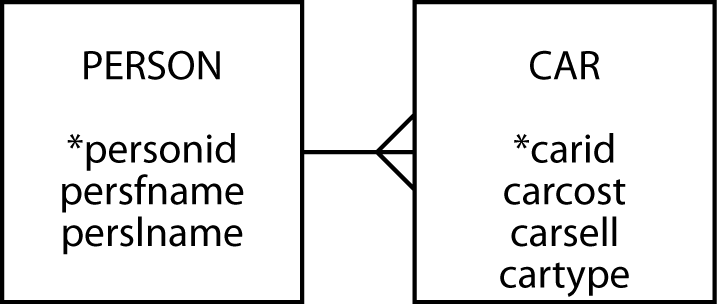
\includegraphics[width=3.48958in,height=\textheight]{Figures/Chapter 4/person-car.png}

\begin{enumerate}
\def\labelenumi{\arabic{enumi}.}
\setcounter{enumi}{7}
\item
  Answer the following queries based on the following database for a
  car dealer:

  \begin{enumerate}
  \def\labelenumii{\alph{enumii}.}
  \item
    What is the personid of Sheila O'Hara?
  \item
    List sales personnel sorted by last name and within last name,
    first name.
  \item
    List details of the sales made by Bruce Bush.
  \item
    List details of all sales showing the gross profit (selling
    price minus cost price).
  \item
    Report the number of cars sold of each type.
  \item
    What is the average selling price of cars sold by Sue Lim?
  \item
    Report details of all sales where the gross profit is less than
    the average.
  \item
    What was the maximum selling price of any car?
  \item
    What is the total gross profit?
  \item
    Report the gross profit made by each salesperson who sold at
    least three cars.
  \item
    Create a view containing all the details in the car table and
    the gross profit
  \end{enumerate}
\item
  Find stocks where the third or fourth letter in their name is an
  `m'.
\item
  An electricity supply company needs a database to record details of
  solar panels installed on its customers' homes so it can estimate
  how much solar energy will be generated based on the forecast level
  of solar radiation for each house's location. A solar panel has an
  area, measured in square meters, and an efficiency expressed as a
  percentage (e.g., 22\% efficiency means that 22\% of the incident
  solar energy is converted into electrical energy). Create a data
  model. How will you identify each customer and each panel?
\end{enumerate}

\hypertarget{the-many-to-many-relationship}{%
\section{The Many-to-Many Relationship}\label{the-many-to-many-relationship}}

\begin{quote}
\emph{Fearful concatenation of circumstances.}

Daniel Webster
\end{quote}

\hypertarget{learning-objectives-4}{%
\subsubsection*{Learning objectives}\label{learning-objectives-4}}
\addcontentsline{toc}{subsubsection}{Learning objectives}

Students completing this chapter will be able to

\begin{itemize}
\item
  model a many-to-many relationship between two entities;
\item
  define a database with a many-to-many relationship;
\item
  write queries for a database with a many-to-many relationship.
\end{itemize}

\hypertarget{the-many-to-many-relationship-1}{%
\subsection*{The many-to-many relationship}\label{the-many-to-many-relationship-1}}
\addcontentsline{toc}{subsection}{The many-to-many relationship}

Consider the case when items are sold. We can immediately identify two entities: SALE and ITEM. A sale can contain many items, and an item can appear in many sales. We are not saying the same item can be sold many times, but the particular type of item (e.g., a compass) can be sold many times; thus we have a many-to-many (m:m) relationship between SALE and ITEM. When we have an m:m relationship, we create a third entity to link the entities through two 1:m relationships. Usually, it is fairly easy to name this third entity. In this case, this third entity, typically known as an \textbf{associative entity}, is called LINE ITEM. A typical old style sales form lists the items purchased by a customer. Each of the lines appearing on the order form is generally known in retailing as a line item, which links an item and a sale.

\emph{A sales form} 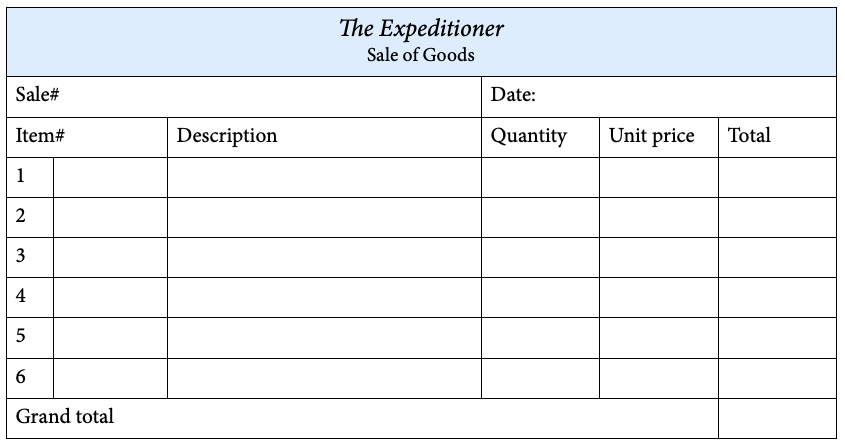
\includegraphics{Figures/Chapter 5/sales form.png}

The representation of this m:m relationship is shown. We say many-to-many because there are two relationships---an ITEM is related to many SALEs, and a SALE is related to many ITEMs. This data model can also be read as: ``a sale has many line items, but a line item refers to only one sale. Similarly, an item can appear as many line items, but a line item references only one item.''

\emph{An m:m relationship between SALE and ITEM}

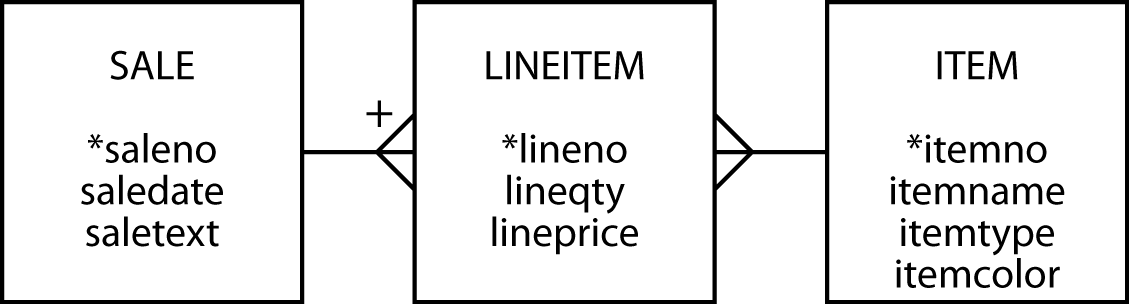
\includegraphics[width=5.89583in,height=\textheight]{Figures/Chapter 5/sale-item.png}

The entity SALE is identified by \emph{saleno} and has the attributes \emph{saledate} and \emph{saletext} (a brief comment on the customer---soft information). LINEITEM is partially identified by \emph{lineno} and has attributes \emph{lineqty} (the number of units sold) and \emph{lineprice} (the unit selling price for this sale). ITEM is identified by \emph{itemno} and has attributes \emph{itemname}, \emph{itemtype} (e.g., clothing, equipment, navigation aids, furniture, and so on), and \emph{itemcolor}.

If you look carefully at the m:m relationship figure, you will notice that there is a plus sign (+) above the crow's foot at the ``many'' end of the 1:m relationship between SALE and LINEITEM. This plus sign provides information about the identifier of LINEITEM. As you know, every entity must have a unique identifier. A sales order is a series of rows or lines, and \emph{lineno} is unique only within a particular order. If we just use \emph{lineno} as the identifier, we cannot guarantee that every instance of LINEITEM is unique. If we use \emph{saleno} and \emph{lineno} together, however, we have a unique identifier for every instance of LINEITEM. Identifier \emph{saleno} is unique for every sale, and \emph{lineno} is unique within any sale. The plus indicates that LINEITEM's unique identifier is the concatenation of \emph{saleno} and \emph{lineno}. The order of concatenation does not matter.

LINEITEM is termed a \textbf{weak entity} because it relies on another entity for its existence and identification.

\hypertarget{mysql-workbench-1}{%
\subsubsection*{MySQL Workbench}\label{mysql-workbench-1}}
\addcontentsline{toc}{subsubsection}{MySQL Workbench}

Workbench automatically creates an associative entity for an m:m relationship and populates it with a composite primary key based on concatenating the primary keys of the two entities forming the m:m relationship. \emph{First}, draw the two tables and enter their respective primary keys and columns. \emph{Second}, select the m:m symbol and connect the two tables through clicking on one and dragging to the second and releasing. You can then modify the associative entity as required, such as changing its primary key. The capability to automatically create an associative entity for an m:m relationship is a very useful Workbench feature.

\emph{An m:m relationship with Workbench}

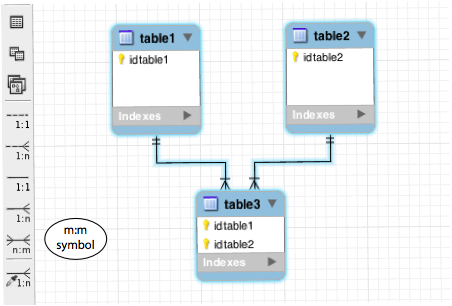
\includegraphics{Figures/Chapter 5/m-m-wb.png}

Workbench distinguishes between two types of relationships. An \textbf{identifying relationship}, shown by a solid line, is used when the entity at the many end of the relationship is a weak entity and needs the identifier of the one end of the relationship to uniquely identify an instance of the relationship, as in LINEITEM. An identifying relationship corresponds to the + sign associated with a crow's foot. The other type of relationship, shown by a dashed line, is known as a \emph{non-identifying} relationship. The mapping between the type of relationship and the representation (i.e., dashed or solid line) is arbitrary and thus not always easily recalled. We think that using a + on the crow's foot is a better way of denoting weak entities.

When the relationship between SALE and ITEM is drawn in Workbench, as shown in the following figure, there are two things to notice. \emph{First}, the table, lineitem, maps the associative entity generated for the m:m relationship. \emph{Second}, lineitem has an identifying relationship with sale and a non-identifying relationship with item.

\emph{An m:m relationship between SALE and ITEM in MySQL Workbench}

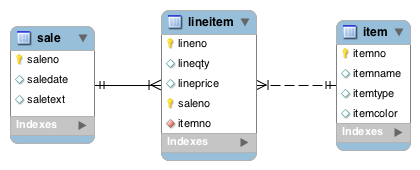
\includegraphics{Figures/Chapter 5/sale-item-wb.png}

\hypertarget{why-did-we-create-a-third-entity}{%
\subsubsection*{Why did we create a third entity?}\label{why-did-we-create-a-third-entity}}
\addcontentsline{toc}{subsubsection}{Why did we create a third entity?}

When we have an m:m relationship, we create an associative entity to store data about the relationship. In this case, we have to store data about the items sold. We cannot store the data with SALE because a sale can have many items, and an instance of an entity stores only single-value facts. Similarly, we cannot store data with ITEM because an item can appear in many sales. Since we cannot store data in SALE or ITEM, we must create another entity to store data about the m:m relationship.

You might find it useful to think of the m:m relationship as two 1:m relationships. An item can appear on many line item listings, and a line item entry refers to only one item. A sale has many line items, and each line item entry refers to only one sale.

\begin{quote}
\textbf{\emph{Social Security number is notunique!}}

Two girls named Sarah Lee Ferguson were born on May 3, 1959. The U.S. government considered them one and the same and issued both the same Social Security number (SSN), a nine-digit identifier of U.S. residents. Now Sarah Lee Ferguson Boles and Sarah Lee Ferguson Johnson share the same SSN.\footnote{``Two women share a name, birthday, and S.S. number!'' Athens Daily News, January 29 1990, 7A. Also, see \textgreater{} \url{https://www.computerworld.com/article/3004659/a-tale-of-two-women-same-birthday-same-social-security-number-same-big-data-mess.html}}

Mrs.~Boles became aware of her SSN twin in 1987 when the Internal Revenue Service claimed there was a discrepancy in her reported income Because SSN is widely used as an attribute or identifier in many computer systems, Mrs.~Boles encountered other incidents of mistaken identity. Some of Mrs.~Johnson's purchases appeared on Mrs.~Boles' credit reports.

In late 1989, the Social Security Administration notified Mrs.~Boles that her original number was given to her in error and she had to provide evidence of her age, identity, and citizenship to get a new number. When Mrs.~Boles got her new SSN, it is likely she had to also get a new driver's license and establish a new credit history.
\end{quote}

\hypertarget{creating-a-relational-database-with-an-mm-relationship}{%
\subsection*{Creating a relational database with an m:m relationship}\label{creating-a-relational-database-with-an-mm-relationship}}
\addcontentsline{toc}{subsection}{Creating a relational database with an m:m relationship}

As before, each entity becomes a table in a relational database, the entity name becomes the table name, each attribute becomes a column, and each identifier becomes a primary key. Remember, a 1:m relationship is mapped by adding a column to the entity of the many end of the relationship. The new column contains the identifier of the one end of the relationship.

Conversion of the foregoing data model results in the three tables following. Note the one-to-one correspondence between attributes and columns for sale and item. Observe the lineitem has two additional columns, saleno and itemno. Both of these columns are foreign keys in lineitem (remember the use of italics to signify foreign keys). Two foreign keys are required to record the two 1:m relationships. Notice in lineitem that saleno is both part of the primary key and a foreign key.

\emph{Tables sale, lineitem, and item}

\begin{longtable}[]{@{}lll@{}}
\toprule
\underline{saleno} & saledate & saletext \\
\midrule
\endhead
1 & 2020-01-15 & Scruffy Australian---called himself Bruce. \\
2 & 2020-01-15 & Man. Rather fond of hats. \\
3 & 2020-01-15 & Woman. Planning to row Atlantic---lengthwise! \\
4 & 2020-01-15 & Man. Trip to New York---thinks NY is a jungle! \\
5 & 2020-01-16 & Expedition leader for African safari. \\
\bottomrule
\end{longtable}

\begin{longtable}[]{@{}lrrrr@{}}
\toprule
\underline{lineno} & lineqty & lineprice & \underline{\emph{saleno}} & \emph{itemno} \\
\midrule
\endhead
1 & 1 & 4.50 & 1 & 2 \\
1 & 1 & 25.00 & 2 & 6 \\
2 & 1 & 20.00 & 2 & 16 \\
3 & 1 & 25.00 & 2 & 19 \\
4 & 1 & 2.25 & 2 & 2 \\
1 & 1 & 500.00 & 3 & 4 \\
2 & 1 & 2.25 & 3 & 2 \\
1 & 1 & 500.00 & 4 & 4 \\
2 & 1 & 65.00 & 4 & 9 \\
3 & 1 & 60.00 & 4 & 13 \\
4 & 1 & 75.00 & 4 & 14 \\
5 & 1 & 10.00 & 4 & 3 \\
6 & 1 & 2.25 & 4 & 2 \\
1 & 50 & 36.00 & 5 & 10 \\
2 & 50 & 40.50 & 5 & 11 \\
3 & 8 & 153.00 & 5 & 12 \\
4 & 1 & 60.00 & 5 & 13 \\
5 & 1 & 0.00 & 5 & 2 \\
\bottomrule
\end{longtable}

\begin{longtable}[]{@{}llll@{}}
\toprule
\underline{itemno} & itemname & itemtype & itemcolor \\
\midrule
\endhead
1 & Pocket knife---Nile & E & Brown \\
2 & Pocket knife---Avon & E & Brown \\
3 & Compass & N & --- \\
4 & Geopositioning system & N & --- \\
5 & Map measure & N & --- \\
6 & Hat---Polar Explorer & C & Red \\
7 & Hat---Polar Explorer & C & White \\
8 & Boots---snake proof & C & Green \\
9 & Boots---snake proof & C & Black \\
10 & Safari chair & F & Khaki \\
11 & Hammock & F & Khaki \\
12 & Tent---8 person & F & Khaki \\
13 & Tent---2 person & F & Khaki \\
14 & Safari cooking kit & E & --- \\
15 & Pith helmet & C & Khaki \\
16 & Pith helmet & C & White \\
17 & Map case & N & Brown \\
18 & Sextant & N & --- \\
19 & Stetson & C & Black \\
20 & Stetson & C & Brown \\
\bottomrule
\end{longtable}

The SQL commands to create the three tables are as follows:

\begin{Shaded}
\begin{Highlighting}[]
\KeywordTok{CREATE} \KeywordTok{TABLE}\NormalTok{ sale (}
\NormalTok{    saleno      }\DataTypeTok{INTEGER}\NormalTok{,}
\NormalTok{    saledate        }\DataTypeTok{DATE} \KeywordTok{NOT} \KeywordTok{NULL}\NormalTok{,}
\NormalTok{    saletext        }\DataTypeTok{VARCHAR}\NormalTok{(}\DecValTok{50}\NormalTok{),}
      \KeywordTok{PRIMARY} \KeywordTok{KEY}\NormalTok{(saleno));}
\end{Highlighting}
\end{Shaded}

\begin{Shaded}
\begin{Highlighting}[]
\KeywordTok{CREATE} \KeywordTok{TABLE}\NormalTok{ item (}
\NormalTok{    itemno      }\DataTypeTok{INTEGER}\NormalTok{,}
\NormalTok{    itemname        }\DataTypeTok{VARCHAR}\NormalTok{(}\DecValTok{30}\NormalTok{) }\KeywordTok{NOT} \KeywordTok{NULL}\NormalTok{,}
\NormalTok{    itemtype        }\DataTypeTok{CHAR}\NormalTok{(}\DecValTok{1}\NormalTok{) }\KeywordTok{NOT} \KeywordTok{NULL}\NormalTok{,}
\NormalTok{    itemcolor       }\DataTypeTok{VARCHAR}\NormalTok{(}\DecValTok{10}\NormalTok{),}
        \KeywordTok{PRIMARY} \KeywordTok{KEY}\NormalTok{(itemno));}
\end{Highlighting}
\end{Shaded}

\begin{Shaded}
\begin{Highlighting}[]
\KeywordTok{CREATE} \KeywordTok{TABLE}\NormalTok{ lineitem (}
\NormalTok{    lineno      }\DataTypeTok{INTEGER}\NormalTok{,}
\NormalTok{    lineqty     }\DataTypeTok{INTEGER} \KeywordTok{NOT} \KeywordTok{NULL}\NormalTok{,}
\NormalTok{    lineprice       }\DataTypeTok{DECIMAL}\NormalTok{(}\DecValTok{7}\NormalTok{,}\DecValTok{2}\NormalTok{) }\KeywordTok{NOT} \KeywordTok{NULL}\NormalTok{,}
\NormalTok{    saleno      }\DataTypeTok{INTEGER}\NormalTok{,}
\NormalTok{    itemno      }\DataTypeTok{INTEGER}\NormalTok{,}
        \KeywordTok{PRIMARY} \KeywordTok{KEY}\NormalTok{(lineno,saleno),}
        \KeywordTok{CONSTRAINT}\NormalTok{ fk\_has\_sale }\KeywordTok{FOREIGN} \KeywordTok{KEY}\NormalTok{(saleno)}
            \KeywordTok{REFERENCES}\NormalTok{ sale(saleno),}
        \KeywordTok{CONSTRAINT}\NormalTok{ fk\_has\_item }\KeywordTok{FOREIGN} \KeywordTok{KEY}\NormalTok{(itemno)}
            \KeywordTok{REFERENCES}\NormalTok{ item(itemno));}
\end{Highlighting}
\end{Shaded}

Although the \texttt{sale} and \texttt{item} tables are created in a similar fashion to previous examples, there are two things to note about the definition of \texttt{lineitem}. \emph{First,} the primary key is a composite of \texttt{lineno} and \texttt{saleno}, because together they uniquely identify an instance of \texttt{lineitem}. \emph{Second}, there are two foreign keys, because \texttt{lineno} is at the ``many'' end of two 1: m relationships.

\begin{quote}
❓\emph{Skill builder}

A hamburger shop makes several types of hamburgers, and the same type of ingredient can be used with several types of hamburgers. This does not literally mean the same piece of lettuce is used many times, but lettuce is used with several types of hamburgers. Draw the data model for this situation. What is a good name for the associative entity?
\end{quote}

\hypertarget{querying-an-mm-relationship}{%
\subsection*{Querying an m:m relationship}\label{querying-an-mm-relationship}}
\addcontentsline{toc}{subsection}{Querying an m:m relationship}

\hypertarget{a-three-table-join}{%
\subsubsection*{A three-table join}\label{a-three-table-join}}
\addcontentsline{toc}{subsubsection}{A three-table join}

The join operation can be easily extended from two tables to three or more merely by specifying the tables to be joined and the matching conditions. For example:

\begin{Shaded}
\begin{Highlighting}[]
\KeywordTok{SELECT} \OperatorTok{*} \KeywordTok{FROM}\NormalTok{ sale }\KeywordTok{JOIN}\NormalTok{ lineitem }
    \KeywordTok{ON}\NormalTok{ sale.saleno }\OperatorTok{=}\NormalTok{ lineitem.saleno}
    \KeywordTok{JOIN}\NormalTok{ item}
    \KeywordTok{ON}\NormalTok{ item.itemno }\OperatorTok{=}\NormalTok{ lineitem.itemno;}
\end{Highlighting}
\end{Shaded}

There are two matching conditions: one for \texttt{sale} and \texttt{lineitem} (\texttt{sale.saleno} = \texttt{lineitem.saleno}) and one for the item and \texttt{lineitem} tables (\texttt{item.itemno} = \texttt{lineitem.itemno}). The table \texttt{lineitem} is the link between \texttt{sale} and \texttt{item} and must be referenced in both matching conditions.

You can tailor the join to be more precise and report some columns rather than all.

\emph{List the name, quantity, price, and value of items sold on January 16, 2011.}

\begin{Shaded}
\begin{Highlighting}[]
\KeywordTok{SELECT}\NormalTok{ itemname, lineqty, lineprice, lineqty}\OperatorTok{*}\NormalTok{lineprice }\KeywordTok{AS}\NormalTok{ total}
    \KeywordTok{FROM}\NormalTok{ sale, lineitem, item}
        \KeywordTok{WHERE}\NormalTok{ lineitem.saleno }\OperatorTok{=}\NormalTok{ sale.saleno}
        \KeywordTok{AND}\NormalTok{ item.itemno }\OperatorTok{=}\NormalTok{ lineitem.itemno}
        \KeywordTok{AND}\NormalTok{ saledate }\OperatorTok{=} \StringTok{\textquotesingle{}2011{-}01{-}16\textquotesingle{}}\NormalTok{;}
\end{Highlighting}
\end{Shaded}

\begin{table}

\caption{\label{tab:unnamed-chunk-63}5 records}
\centering
\begin{tabular}[t]{l|r|r|r}
\hline
itemname & lineqty & lineprice & total\\
\hline
Safari chair & 50 & 36.0 & 1800\\
\hline
Hammock & 50 & 40.5 & 2025\\
\hline
Tent - 8 person & 8 & 153.0 & 1224\\
\hline
Tent - 2 person & 1 & 60.0 & 60\\
\hline
Pocket knife - Avon & 1 & 0.0 & 0\\
\hline
\end{tabular}
\end{table}

\hypertarget{existsdoes-a-value-exist}{%
\subsubsection*{EXISTS---does a value exist}\label{existsdoes-a-value-exist}}
\addcontentsline{toc}{subsubsection}{EXISTS---does a value exist}

EXISTS is used in a WHERE clause to test whether a table contains at least one row satisfying a specified condition. It returns the value \textbf{true} if and only if some row satisfies the condition; otherwise it returns \textbf{false}. EXISTS represents the \textbf{existential quantifier} of formal logic. The best way to get a feel for EXISTS is to examine a query.

\emph{Report all clothing items (type ``C'') for which a sale is recorded.}

\begin{Shaded}
\begin{Highlighting}[]
\KeywordTok{SELECT}\NormalTok{ itemname, itemcolor }\KeywordTok{FROM}\NormalTok{ item}
    \KeywordTok{WHERE}\NormalTok{ itemtype }\OperatorTok{=} \StringTok{\textquotesingle{}C\textquotesingle{}}
    \KeywordTok{AND} \KeywordTok{EXISTS}\NormalTok{ (}\KeywordTok{SELECT} \OperatorTok{*} \KeywordTok{FROM}\NormalTok{ lineitem}
        \KeywordTok{WHERE}\NormalTok{ lineitem.itemno }\OperatorTok{=}\NormalTok{ item.itemno);}
\end{Highlighting}
\end{Shaded}

\begin{table}

\caption{\label{tab:unnamed-chunk-64}4 records}
\centering
\begin{tabular}[t]{l|l}
\hline
itemname & itemcolor\\
\hline
Hat - Polar explorer & Red\\
\hline
Boots - snake proof & Black\\
\hline
Pith helmet & White\\
\hline
Stetson & Black\\
\hline
\end{tabular}
\end{table}

Conceptually, we can think of this query as evaluating the subquery for each row of item. The first item with itemtype = `C', Hat---Polar Explorer (red), in item has itemno = 6. Thus, the query becomes

\begin{Shaded}
\begin{Highlighting}[]
\KeywordTok{SELECT}\NormalTok{ itemname, itemcolor }\KeywordTok{FROM}\NormalTok{ item}
    \KeywordTok{WHERE}\NormalTok{ itemtype }\OperatorTok{=} \StringTok{\textquotesingle{}C\textquotesingle{}}
    \KeywordTok{AND} \KeywordTok{EXISTS}\NormalTok{ (}\KeywordTok{SELECT} \OperatorTok{*} \KeywordTok{FROM}\NormalTok{ lineitem}
        \KeywordTok{WHERE}\NormalTok{ lineitem.itemno }\OperatorTok{=} \DecValTok{6}\NormalTok{);}
\end{Highlighting}
\end{Shaded}

Because there is at least one row in \texttt{lineitem} with \texttt{itemno} = 6, the subquery returns \emph{true}. The item has been sold and should be reported. The second clothing item, Hat---Polar Explorer (white), in \texttt{item} has \texttt{itemno} = 7. There are no rows in \texttt{lineitem} with \texttt{itemno} = 7, so the subquery returns \emph{false}. That item has not been sold and should not be reported.

You can also think of the query as, ``Select clothing items for which a sale exists.'' Remember, for EXISTS to return \emph{true}, there needs to be only one row for which the condition is \emph{true}.

\hypertarget{not-existsselect-a-value-if-it-does-not-exist}{%
\subsubsection*{NOT EXISTS---select a value if it does not exist}\label{not-existsselect-a-value-if-it-does-not-exist}}
\addcontentsline{toc}{subsubsection}{NOT EXISTS---select a value if it does not exist}

NOT EXISTS is the negative of EXISTS. It is used in a WHERE clause to test whether all rows in a table fail to satisfy a specified condition. It returns the value \emph{true} if there are no rows satisfying the condition; otherwise it returns \emph{false}.

\emph{Report all clothing items that have not been sold.}

\begin{Shaded}
\begin{Highlighting}[]
\KeywordTok{SELECT}\NormalTok{ itemname, itemcolor }\KeywordTok{FROM}\NormalTok{ item}
    \KeywordTok{WHERE}\NormalTok{ itemtype }\OperatorTok{=} \StringTok{\textquotesingle{}C\textquotesingle{}}
    \KeywordTok{AND} \KeywordTok{NOT} \KeywordTok{EXISTS}
\NormalTok{        (}\KeywordTok{SELECT} \OperatorTok{*} \KeywordTok{FROM}\NormalTok{ lineitem}
            \KeywordTok{WHERE}\NormalTok{ item.itemno }\OperatorTok{=}\NormalTok{ lineitem.itemno);}
\end{Highlighting}
\end{Shaded}

\begin{table}

\caption{\label{tab:unnamed-chunk-66}4 records}
\centering
\begin{tabular}[t]{l|l}
\hline
itemname & itemcolor\\
\hline
Hat - Polar explorer & White\\
\hline
Boots - snake proof & Green\\
\hline
Pith helmet & Khaki\\
\hline
Stetson & Brown\\
\hline
\end{tabular}
\end{table}

You can also think of the query as, ``Select clothing items for which no sales exist.'' Also remember, for NOT EXISTS to return \emph{true}, no rows should satisfy the condition.

\begin{quote}
❓\emph{Skill builder}

Report all red items that have not been sold. Write the query twice, once using EXISTS and once without EXISTS.
\end{quote}

\hypertarget{divide-and-be-conquered}{%
\subsubsection*{Divide (and be conquered)}\label{divide-and-be-conquered}}
\addcontentsline{toc}{subsubsection}{Divide (and be conquered)}

In addition to the existential quantifier that you have already encountered, formal logic has a \textbf{universal quantifier} known as \textbf{forall} that is necessary for queries such as

Find the items that have appeared in all sales.

If a universal quantifier were supported by SQL, this query could be phrased as, ``Select item names where \emph{forall} sales there \emph{exists} a \texttt{lineitem} row recording that this item was sold.'' A quick inspection of the first set of tables shows that one item satisfies this condition (\texttt{itemno} = 2).

While SQL does not directly support the universal quantifier, formal logic shows that \emph{forall} can be expressed using EXISTS. The query becomes, ``Find items such that there does not exist a sale in which this item does not appear.'' The equivalent SQL expression is

\begin{Shaded}
\begin{Highlighting}[]
\KeywordTok{SELECT}\NormalTok{ itemno, itemname }\KeywordTok{FROM}\NormalTok{ item}
    \KeywordTok{WHERE} \KeywordTok{NOT} \KeywordTok{EXISTS}
\NormalTok{        (}\KeywordTok{SELECT} \OperatorTok{*} \KeywordTok{FROM}\NormalTok{ sale}
            \KeywordTok{WHERE} \KeywordTok{NOT} \KeywordTok{EXISTS}
\NormalTok{                (}\KeywordTok{SELECT} \OperatorTok{*} \KeywordTok{FROM}\NormalTok{ lineitem}
                    \KeywordTok{WHERE}\NormalTok{ lineitem.itemno }\OperatorTok{=}\NormalTok{ item.itemno}
                    \KeywordTok{AND}\NormalTok{ lineitem.saleno }\OperatorTok{=}\NormalTok{ sale.saleno));}
\end{Highlighting}
\end{Shaded}

\begin{table}

\caption{\label{tab:unnamed-chunk-67}1 records}
\centering
\begin{tabular}[t]{r|l}
\hline
itemno & itemname\\
\hline
2 & Pocket knife - Avon\\
\hline
\end{tabular}
\end{table}

If you are interested in learning the inner workings of the preceding SQL for divide, see the additional material for Chapter 5 on the book's Web site.

Relational algebra (Chapter 9) has the divide operation, which makes divide queries easy to write. Be careful: Not all queries containing the word \emph{all} are divides. With experience, you will learn to recognize and conquer divide.

To save the tedium of formulating this query from scratch, we have developed a template for dealing with these sorts of queries. Divide queries typically occur with m:m relationships.

\emph{A template for divide}

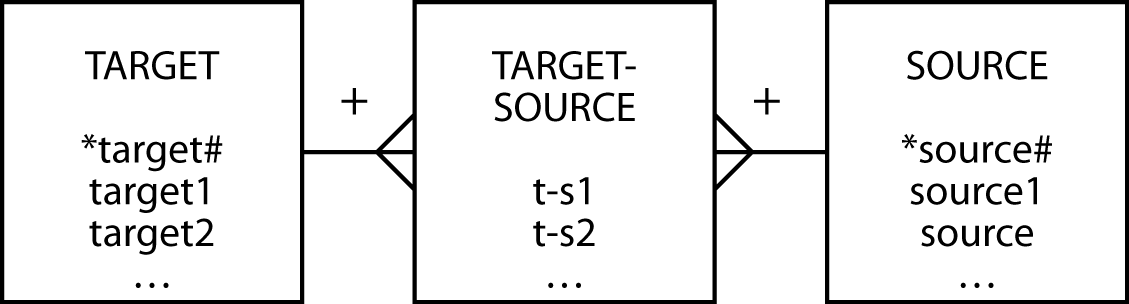
\includegraphics[width=5.89583in,height=\textheight]{Figures/Chapter 5/divide template.png}

An appropriate generic query and template SQL command are

\emph{Find the target1 that have appeared in all sources.}

\begin{Shaded}
\begin{Highlighting}[]
\KeywordTok{SELECT}\NormalTok{ target1 }\KeywordTok{FROM}\NormalTok{ target}
    \KeywordTok{WHERE} \KeywordTok{NOT} \KeywordTok{EXISTS}
\NormalTok{        (}\KeywordTok{SELECT} \OperatorTok{*} \KeywordTok{FROM} \KeywordTok{source}
            \KeywordTok{WHERE} \KeywordTok{NOT} \KeywordTok{EXISTS}
\NormalTok{                (}\KeywordTok{SELECT} \OperatorTok{*} \KeywordTok{FROM}\NormalTok{ target}\OperatorTok{{-}}\KeywordTok{source}
                    \KeywordTok{WHERE}\NormalTok{ target}\OperatorTok{{-}}\KeywordTok{source}\NormalTok{.target\# }\OperatorTok{=}\NormalTok{ target.target\#}
                    \KeywordTok{AND}\NormalTok{ target}\OperatorTok{{-}}\KeywordTok{source}\NormalTok{.source\# }\OperatorTok{=} \KeywordTok{source}\NormalTok{.source\#));}
\end{Highlighting}
\end{Shaded}

\begin{quote}
❓\emph{Skill builder}

Find the brown items that have appeared in all sales.
\end{quote}

\hypertarget{beyond-the-great-divide}{%
\subsubsection*{Beyond the great divide}\label{beyond-the-great-divide}}
\addcontentsline{toc}{subsubsection}{Beyond the great divide}

Divide proves troublesome to most people because of the double negative---we just don't think that way. If divide sends your neurons into knots, then try the following approach.

The query ``Find the items that have appeared in all sales'' can be rephrased as ``Find the items for which the number of sales that include this item is equal to the total number of sales.'' This is an easier query to write than ``Find items such that there does not exist a sale in which this item does not appear.'' The rephrased query has two parts. \emph{First\textbf{,}} determine the total number of sales. Here we mean distinct sales (i.e., the number of rows with a distinct value for saleno). The SQL is

\begin{Shaded}
\begin{Highlighting}[]
\KeywordTok{SELECT} \FunctionTok{COUNT}\NormalTok{ (}\KeywordTok{DISTINCT}\NormalTok{ saleno) }\KeywordTok{FROM}\NormalTok{ sale;}
\end{Highlighting}
\end{Shaded}

\emph{Second}, group the items sold by \texttt{itemno} and \texttt{itemname} and use a HAVING clause with COUNT to calculate the number of sales in which the item has occurred. Forcing the count in the HAVING clause to equal the result of the first query, which becomes an inner query, results in a list of items appearing in all sales.

\begin{Shaded}
\begin{Highlighting}[]
\KeywordTok{SELECT}\NormalTok{ item.itemno, item.itemname}
    \KeywordTok{FROM}\NormalTok{ item }\KeywordTok{JOIN}\NormalTok{ lineitem}
        \KeywordTok{ON}\NormalTok{ item.itemno }\OperatorTok{=}\NormalTok{ lineitem.itemno}
            \KeywordTok{GROUP} \KeywordTok{BY}\NormalTok{ item.itemno, item.itemname}
                \KeywordTok{HAVING} \FunctionTok{COUNT}\NormalTok{(}\KeywordTok{DISTINCT}\NormalTok{ saleno)}
                    \OperatorTok{=}\NormalTok{ (}\KeywordTok{SELECT} \FunctionTok{COUNT}\NormalTok{(}\KeywordTok{DISTINCT}\NormalTok{ saleno) }\KeywordTok{FROM}\NormalTok{ sale);}
\end{Highlighting}
\end{Shaded}

\hypertarget{set-operations}{%
\subsubsection*{Set operations}\label{set-operations}}
\addcontentsline{toc}{subsubsection}{Set operations}

Set operators are useful for combining the values derived from two or more SQL queries. The UNION operation is equivalent to \emph{or}, and INTERSECT is equivalent to \emph{and}.

\emph{List items that were sold on January 16, 2011, or are brown.}

Resolution of this query requires two tables: one to report items sold on January 16, 2011, and one to report the brown items. UNION (i.e., or) then combines the results of the tables, including \emph{any} rows in both tables and excluding duplicate rows.

\begin{Shaded}
\begin{Highlighting}[]
\KeywordTok{SELECT}\NormalTok{ itemname }\KeywordTok{FROM}\NormalTok{ item }\KeywordTok{JOIN}\NormalTok{ lineitem}
    \KeywordTok{ON}\NormalTok{ item.itemno }\OperatorTok{=}\NormalTok{ lineitem.itemno}
    \KeywordTok{JOIN}\NormalTok{ sale}
    \KeywordTok{ON}\NormalTok{ lineitem.saleno }\OperatorTok{=}\NormalTok{ sale.saleno}
    \KeywordTok{WHERE}\NormalTok{ saledate }\OperatorTok{=} \StringTok{\textquotesingle{}2011{-}01{-}16\textquotesingle{}}
\KeywordTok{UNION}
    \KeywordTok{SELECT}\NormalTok{ itemname }\KeywordTok{FROM}\NormalTok{ item }\KeywordTok{WHERE}\NormalTok{ itemcolor }\OperatorTok{=} \StringTok{\textquotesingle{}Brown\textquotesingle{}}\NormalTok{;}
\end{Highlighting}
\end{Shaded}

\begin{table}

\caption{\label{tab:unnamed-chunk-71}8 records}
\centering
\begin{tabular}[t]{l}
\hline
itemname\\
\hline
Safari chair\\
\hline
Hammock\\
\hline
Tent - 8 person\\
\hline
Tent - 2 person\\
\hline
Pocket knife - Avon\\
\hline
Pocket knife - Nile\\
\hline
Map case\\
\hline
Stetson\\
\hline
\end{tabular}
\end{table}

\emph{List items that were sold on January 16, 2011, and are brown.}

This query uses the same two tables as the previous query. In this case, INTERSECT (i.e., and) then combines the results of the tables including \textbf{\emph{only}} rows in both tables and excluding duplicates.\footnote{MySQL does not support INTERSECT. Use another AND in the WHERE statement.~}

\begin{Shaded}
\begin{Highlighting}[]
\KeywordTok{SELECT}\NormalTok{ itemname }\KeywordTok{FROM}\NormalTok{ item }\KeywordTok{JOIN}\NormalTok{ lineitem}
    \KeywordTok{ON}\NormalTok{ item.itemno }\OperatorTok{=}\NormalTok{ lineitem.itemno}
    \KeywordTok{JOIN}\NormalTok{ sale}
    \KeywordTok{ON}\NormalTok{ lineitem.saleno }\OperatorTok{=}\NormalTok{ sale.saleno}
    \KeywordTok{WHERE}\NormalTok{ saledate }\OperatorTok{=} \StringTok{\textquotesingle{}2011{-}01{-}16\textquotesingle{}}
\KeywordTok{INTERSECT}
    \KeywordTok{SELECT}\NormalTok{ itemname }\KeywordTok{FROM}\NormalTok{ item }\KeywordTok{WHERE}\NormalTok{ itemcolor }\OperatorTok{=} \StringTok{\textquotesingle{}Brown\textquotesingle{}}\NormalTok{;}
\end{Highlighting}
\end{Shaded}

\begin{quote}
❓\emph{Skill builder}

List the items that contain the words ``Hat'', ``Helmet'', or ``Stetson'' in their names
\end{quote}

\hypertarget{summary-4}{%
\subsection*{Summary}\label{summary-4}}
\addcontentsline{toc}{subsection}{Summary}

There can be a many-to-many (m:m) relationship between entities, which is represented by creating an associative entity and two 1:m relationships. An associative entity stores data about an m:m relationship. The join operation can be extended from two tables to three or more tables. EXISTS tests whether a table has at least one row that meets a specified condition. NOT EXISTS tests whether all rows in a table do not satisfy a specified condition. Both EXISTS and NOT EXISTS can return \emph{true} or \emph{false}. The relational operation divide, also known as \emph{forall}, can be translated into a double negative. It is represented in SQL by a query containing two NOT EXISTS statements. Set operations enable the results of queries to be combined.

\hypertarget{key-terms-and-concepts-2}{%
\subsection*{Key terms and concepts}\label{key-terms-and-concepts-2}}
\addcontentsline{toc}{subsection}{Key terms and concepts}

\begin{longtable}[]{@{}ll@{}}
\toprule
& \\
\midrule
\endhead
Associative entity & Many-to-many (m:m) relationship \\
Divide & NOT EXISTS \\
Existential quantifier & UNION \\
EXISTS & Universal quantifier \\
INTERSECT & \\
\bottomrule
\end{longtable}

\hypertarget{exercises-4}{%
\subsection*{Exercises}\label{exercises-4}}
\addcontentsline{toc}{subsection}{Exercises}

\begin{enumerate}
\def\labelenumi{\arabic{enumi}.}
\item
  Draw data models for the following situations. In each case, think about the names you give each entity:

  \begin{enumerate}
  \def\labelenumii{\alph{enumii}.}
  \item
    Farmers can own cows or share cows with other farmers.
  \item
    A track and field meet can have many competitors, and a competitor can participate in more than one event.
  \item
    A patient can have many physicians, and a physician can have many patients.
  \item
    A student can attend more than one class, and the same class can have many students.
  \item
    \emph{The Marathoner}, a monthly magazine, regularly reports the performance of professional marathon runners. It has asked you to design a database to record the details of all major marathons (e.g., Boston, London, and Paris). Professional marathon runners compete in several races each year. A race may have thousands of competitors, but only about 200 or so are professional runners, the ones \emph{The Marathoner} tracks. For each race, the magazine reports a runner's time and finishing position and some personal details such as name, gender, and age.
  \end{enumerate}
\item
  The data model shown was designed by a golf statistician. Write SQL statements to create the corresponding relational database.
\end{enumerate}

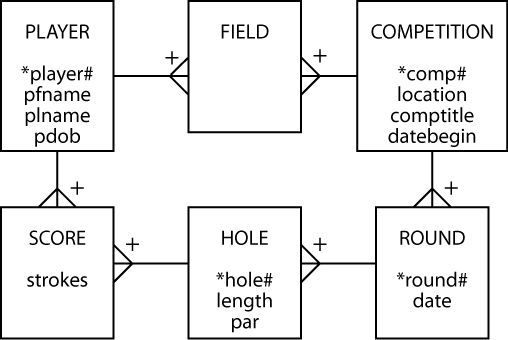
\includegraphics[width=5.44792in,height=\textheight]{Figures/Chapter 5/golf.png}

\begin{enumerate}
\def\labelenumi{\arabic{enumi}.}
\setcounter{enumi}{2}
\item
  Write the following SQL queries for the database described in this chapter:

  \begin{enumerate}
  \def\labelenumii{\alph{enumii}.}
  \item
    List the names of items for which the quantity sold is greater than one for any sale.
  \item
    Compute the total value of sales for each item by date.
  \item
    Report all items of type ``F'' that have been sold.
  \item
    List all items of type ``F'' that have not been sold.
  \item
    Compute the total value of each sale.
  \end{enumerate}
\item
  Why do you have to create a third entity when you have an m:m relationship?
\item
  What does a plus sign near a relationship arc mean?
\item
  How does EXISTS differ from other clauses in an SQL statement?
\item
  Answer the following queries based on the described relational database.

  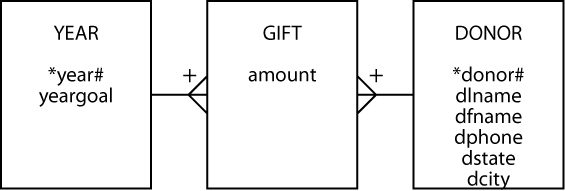
\includegraphics[width=4.61458in,height=\textheight]{Figures/Chapter 5/gift.png}

  \begin{enumerate}
  \def\labelenumii{\alph{enumii}.}
  \item
    List the phone numbers of donors Hays and Jefts.
  \item
    How many donors are there in the donor table?
  \item
    How many people made donations in 1999?
  \item
    What is the name of the person who made the largest donation in 1999?
  \item
    What was the total amount donated in 2000?
  \item
    List the donors who have made a donation every year.
  \item
    List the donors whose average donation is more than twice the average donation of all donors.
  \item
    List the total amount given by each person across all years; sort the report by the donor's name.
  \item
    Report the total donations in 2001 by state.
  \item
    In which years did the total donated exceed the goal for the year?
  \end{enumerate}
\item
  The following table records data found on the side of a breakfast cereal carton. Use these data as a guide to develop a data model to record nutrition facts for a meal. In this case, a meal is a cup of cereal and 1/2 cup of skim milk.
\end{enumerate}

\begin{longtable}[]{@{}
  >{\raggedright\arraybackslash}p{(\columnwidth - 4\tabcolsep) * \real{0.47}}
  >{\raggedright\arraybackslash}p{(\columnwidth - 4\tabcolsep) * \real{0.12}}
  >{\raggedright\arraybackslash}p{(\columnwidth - 4\tabcolsep) * \real{0.39}}@{}}
\toprule
\textbf{Nutrition facts}

Serving size 1 cup (30g)

Servings per container about 17 & & \\
\midrule
\endhead
Amount per serving & Cereal & with 1/2 cup of skim milk \\
Calories & 110 & 150 \\
Calories from Fat & 10 & 10 \\
& & \% Daily Value \\
Total Fat 1g & 1\% & 2\% \\
Saturated Fat 0g & 0\% & 0\% \\
Polyunsaturated Fat 0g & & \\
Monounsaturated Fat 0g & & \\
Cholesterol 0mg & 0\% & 1\% \\
Sodium 220mg & 9\% & 12\% \\
Potassium 105 mg & 3\% & 9\% \\
Total Carbohydrate 24g & 8\% & 10\% \\
Dietary Fiber 3g & 13\% & 13\% \\
Sugars 4g & & \\
Other Carbohydrate 17g & & \\
Protein 3g & & \\
Vitamin A & 10\% & 15\% \\
Vitamin C & 10\% & 10\% \\
Calcium & 2\% & 15\% \\
Iron & 45\% & 45\% \\
Vitamin D & 10\% & 25\% \\
Thiamin & 50\% & 50\% \\
Riboflavin & 50\% & 50\% \\
Niacin & 50\% & 50\% \\
Vitamin B12 & 50\% & 60\% \\
Phosphorus & 10\% & 20\% \\
Magnesium & 8\% & 10\% \\
Zinc & 50\% & 50\% \\
Copper & 4\% & 4\% \\
\bottomrule
\end{longtable}

\hypertarget{one-to-one-and-recursive-relationships}{%
\section{One-to-One and Recursive Relationships}\label{one-to-one-and-recursive-relationships}}

\begin{quote}
\emph{Self-reflection is the school of wisdom.}

Baltasar Gracián, \emph{The Art of Worldly Wisdom}, 1647
\end{quote}

\hypertarget{learning-objectives-5}{%
\subsection*{Learning objectives}\label{learning-objectives-5}}
\addcontentsline{toc}{subsection}{Learning objectives}

Students completing this chapter will be able to

\begin{itemize}
\item
  model one-to-one and recursive relationships;
\item
  define a database with one-to-one and recursive relationships;
\item
  write queries for a database with one-to-one and recursive
  relationships.
\end{itemize}

An organizational chart, as shown in the following diagram, can be
modeled with several relationships.

\emph{The Expeditioner's organizational chart}

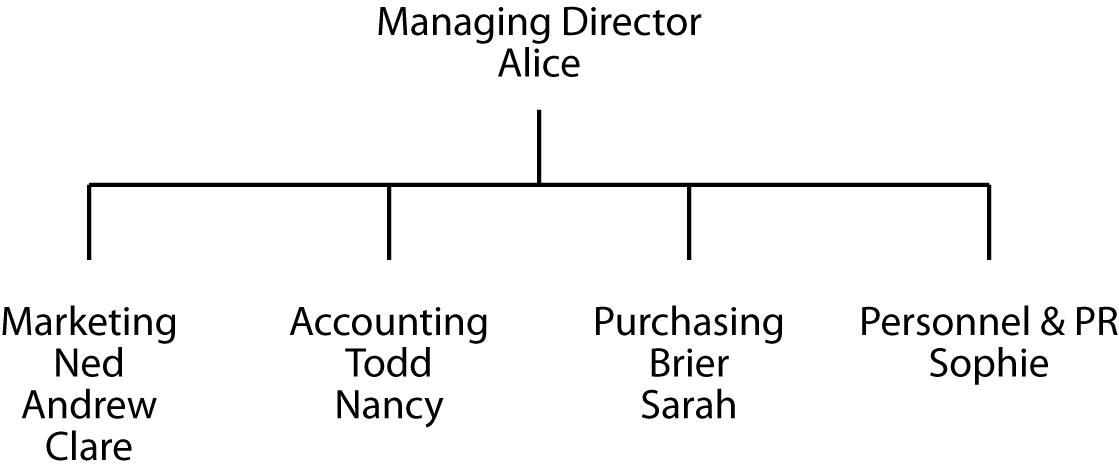
\includegraphics[width=4.95833in,height=\textheight]{Figures/Chapter 6/org chart.png}

\hypertarget{modeling-a-one-to-one-relationship}{%
\subsection*{Modeling a one-to-one relationship}\label{modeling-a-one-to-one-relationship}}
\addcontentsline{toc}{subsection}{Modeling a one-to-one relationship}

Initially, the organization chart appears to record two relationships.
\emph{First\textbf{,}} a department has one or more employees, and an employee
belongs to one department. \emph{Second}, a department has one boss, and a
person is boss of only one department. That is, boss is a 1:1
relationship between DEPT and EMP. The data model for this situation is
shown.

\emph{A data model illustrating a 1:m and 1:1 relationship}

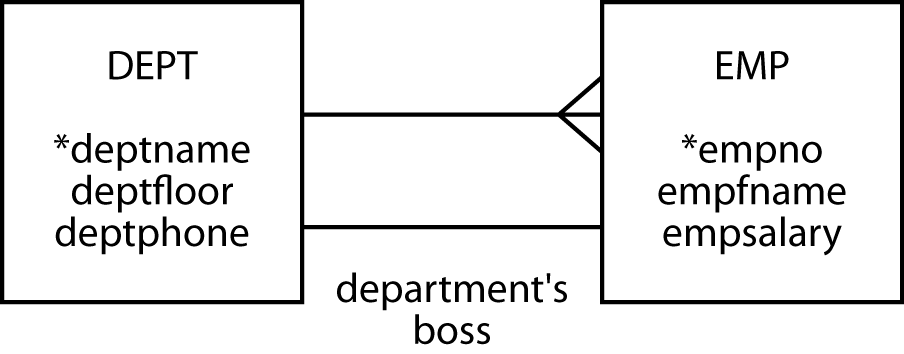
\includegraphics[width=4.70833in,height=\textheight]{Figures/Chapter 6/1-and-1.png}

\emph{MySQL Workbench version of a 1:m and 1:1 relationship}

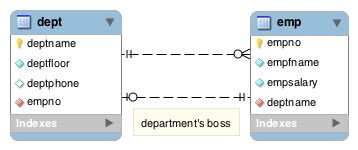
\includegraphics{Figures/Chapter 6/1-1-wb.png}

As a general rule, the 1:1 relationship is labeled to avoid confusion
because the meaning of such a relationship cannot always be inferred.
This label is called a \textbf{relationship descriptor}. The 1:m relationship
between DEPT and EMP is not labeled because its meaning is readily
understood by reading the model. Use a relationship descriptor when
there is more than one relationship between entities or when the meaning
of the relationship is not readily inferred from the model.

If we think about this problem, we realize there is more to boss than
just a department. People also have a boss. Thus, Alice is the boss of
all the other employees. In this case, we are mainly interested in who
directly bosses someone else. So, Alice is the direct boss of Ned, Todd,
Brier, and Sophie. We need to record the person-boss relationship as
well as the department-boss relationship.

The person-boss relationship is a \textbf{recursive 1:m relationship} because
it is a relationship between employees---an employee has one boss and a
boss can have many employees. The data model is shown in the following
figure.

\emph{A data model illustrating a recursive 1:m relationship}

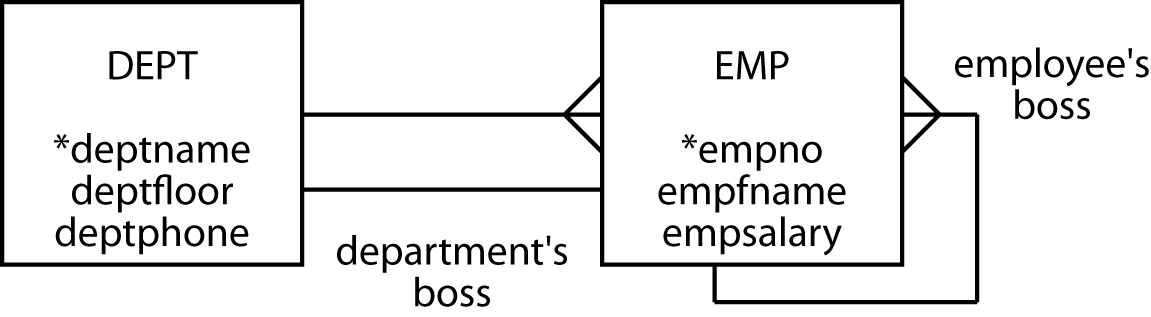
\includegraphics[width=5.67708in,height=\textheight]{Figures/Chapter 6/recursive-1-and-m.png}

\emph{MySQL Workbench version of a recursive 1:m relationship}

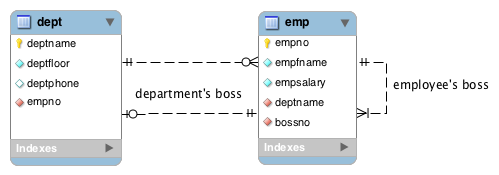
\includegraphics{Figures/Chapter 6/recursive-1-and-m-wb.png}

It is a good idea to label the recursive relationship, because its
meaning is often not obvious from the data model.

\hypertarget{mapping-a-one-to-one-relationship}{%
\subsection*{Mapping a one-to-one relationship}\label{mapping-a-one-to-one-relationship}}
\addcontentsline{toc}{subsection}{Mapping a one-to-one relationship}

Since mapping a 1:1 relationship follows the same rules as for any other
data model, the major consideration is where to place the foreign
key(s). There are three alternatives:

\begin{enumerate}
\def\labelenumi{\arabic{enumi}.}
\item
  Put the foreign key in dept.\\
  Doing so means that every instance of dept will record the empno of
  the employee who is boss. Because it is mandatory that all
  departments, in this case have a boss, the foreign key will always
  be non-null.
\item
  Put the foreign key in emp.\\
  Choosing this alternative means that every instance of emp should
  record deptname of the department this employee bosses. Since many
  employees are not bosses, the value of the foreign key column will
  generally be null.
\item
  Put a foreign key in both dept and emp.\\
  The consequence of putting a foreign key in both tables in the 1:1
  relationship is the combination of points 1 and 2.
\end{enumerate}

The best approach is to put the foreign key in dept, because it is
mandatory for each department to have a boss, and the foreign key will
always be non-null.

\hypertarget{mapping-a-recursive-one-to-many-relationship}{%
\subsection*{Mapping a recursive one-to-many relationship}\label{mapping-a-recursive-one-to-many-relationship}}
\addcontentsline{toc}{subsection}{Mapping a recursive one-to-many relationship}

A recursive 1:m relationship is mapped like a standard 1:m relationship.
An additional column, for the foreign key, is created for the entity at
the ``many'' end of the relationship. Of course, in this case the ``one''
and ``many'' ends are the same entity, so an additional column is added to
\texttt{emp}. This column contains the key \texttt{empno} of the ``one'' end of the
relationship. Since \texttt{empno} is already used as a column name, a
different name needs to be selected. In this case, it makes sense to
call the foreign key column \texttt{bossno} because it stores the boss's
employee number.

The mapping of the data model is shown in the following table. Note that
\texttt{deptname} becomes a column in \texttt{emp}, the ``many'' end of the 1:m
relationship, and \texttt{empno} becomes a foreign key in \texttt{dept}, an end of the
1:1 relationship.

\emph{The tables dept and emp}

\begin{longtable}[]{@{}lccc@{}}
\toprule
\underline{deptname} & deptfloor & deptphone & \emph{empno} \\
\midrule
\endhead
Management & 5 & 2001 & 1 \\
Marketing & 1 & 2002 & 2 \\
Accounting & 4 & 2003 & 5 \\
Purchasing & 4 & 2004 & 7 \\
Personnel \& PR & 1 & 2005 & 9 \\
\bottomrule
\end{longtable}

\begin{longtable}[]{@{}clrlc@{}}
\toprule
\underline{empno} & empfname & empsalary & deptname & bossno \\
\midrule
\endhead
1 & \emph{Alice} & 75000 & \emph{Management} & \\
2 & \emph{Ned} & 45000 & \emph{Marketing} & 1 \\
3 & \emph{Andrew} & 25000 & \emph{Marketing} & 2 \\
4 & \emph{Clare} & 22000 & \emph{Marketing} & 2 \\
5 & \emph{Todd} & 38000 & \emph{Accounting} & 1 \\
6 & \emph{Nancy} & 22000 & \emph{Accounting} & 5 \\
7 & \emph{Brier} & 43000 & \emph{Purchasing} & 1 \\
8 & \emph{Sarah} & 56000 & \emph{Purchasing} & 7 \\
9 & \emph{Sophie} & 35000 & \emph{Personnel \& PR} & 1 \\
\bottomrule
\end{longtable}

If you examine \texttt{emp}, you will see that the boss of the employee with
\texttt{empno} = 2 (Ned) has \texttt{bossno} = 1. You can then look up the row in
\texttt{emp} with \texttt{empno} = 1 to find that Ned's boss is Alice. This ``double
lookup'' is frequently used when manually interrogating a table that
represents a recursive relationship. Soon you will discover how this is
handled with SQL.

Here is the SQL to create the two tables:

\begin{Shaded}
\begin{Highlighting}[]
\KeywordTok{CREATE} \KeywordTok{TABLE}\NormalTok{ dept (}
\NormalTok{    deptname        }\DataTypeTok{VARCHAR}\NormalTok{(}\DecValTok{15}\NormalTok{),}
\NormalTok{    deptfloor       }\DataTypeTok{SMALLINT} \KeywordTok{NOT} \KeywordTok{NULL}\NormalTok{,}
\NormalTok{    deptphone       }\DataTypeTok{SMALLINT} \KeywordTok{NOT} \KeywordTok{NULL}\NormalTok{,}
\NormalTok{    empno           }\DataTypeTok{SMALLINT} \KeywordTok{NOT} \KeywordTok{NULL}\NormalTok{,}
    \KeywordTok{PRIMARY} \KeywordTok{KEY}\NormalTok{(deptname));}
\end{Highlighting}
\end{Shaded}

\begin{Shaded}
\begin{Highlighting}[]
\KeywordTok{CREATE} \KeywordTok{TABLE}\NormalTok{ emp (}
\NormalTok{    empno           }\DataTypeTok{SMALLINT}\NormalTok{,}
\NormalTok{    empfname        }\DataTypeTok{VARCHAR}\NormalTok{(}\DecValTok{10}\NormalTok{),}
\NormalTok{    empsalary       }\DataTypeTok{DECIMAL}\NormalTok{(}\DecValTok{7}\NormalTok{,}\DecValTok{0}\NormalTok{),}
\NormalTok{    deptname        }\DataTypeTok{VARCHAR}\NormalTok{(}\DecValTok{15}\NormalTok{),}
\NormalTok{    bossno          }\DataTypeTok{SMALLINT}\NormalTok{,}
    \KeywordTok{PRIMARY} \KeywordTok{KEY}\NormalTok{(empno),}
    \KeywordTok{CONSTRAINT}\NormalTok{ fk\_belong\_dept }\KeywordTok{FOREIGN} \KeywordTok{KEY}\NormalTok{(deptname) }
        \KeywordTok{REFERENCES}\NormalTok{ dept(deptname),}
    \KeywordTok{CONSTRAINT}\NormalTok{ fk\_has\_boss }\KeywordTok{FOREIGN} \KeywordTok{KEY}\NormalTok{(bossno) }
        \KeywordTok{REFERENCES}\NormalTok{ emp(empno));}
\end{Highlighting}
\end{Shaded}

You will notice that there is no foreign key definition for \texttt{empno} in
\texttt{dept} (the 1:1 department's boss relationship). Why? Observe that
\texttt{deptname} is a foreign key in \texttt{emp}. If we make \texttt{empno} a foreign key
in \texttt{dept}, then we have a \emph{deadly embrace}. A new department cannot be
added to the \texttt{dept} table until there is a boss for that department
(i.e., there is a person in the \texttt{emp} table with the \texttt{empno} of the
boss); however, the other constraint states that an employee cannot be
added to the \texttt{emp} table unless there is a department to which that
person is assigned. If we have both foreign key constraints, we cannot
add a new department until we have added a boss, and we cannot add a
boss until we have added a department for that person. Nothing, under
these circumstances, can happen if both foreign key constraints are in
place. Thus, only one of them is specified.

In the case of the recursive employee relationship, we can create a
constraint to ensure that \texttt{bossno} exists for each employee, except of
course the person, Alice, who is top of the pyramid. This form of
constraint is known as a \textbf{self-referential} foreign key. However, we
must make certain that the first person inserted into \texttt{emp} is Alice.
The following statements illustrate that we must always insert a
person's boss before we insert the person.

\begin{Shaded}
\begin{Highlighting}[]
\KeywordTok{INSERT} \KeywordTok{INTO}\NormalTok{ emp (empno, empfname, empsalary, deptname) }\KeywordTok{VALUES}\NormalTok{ (}\DecValTok{1}\NormalTok{,}\StringTok{\textquotesingle{}Alice\textquotesingle{}}\NormalTok{,}\DecValTok{75000}\NormalTok{,}\StringTok{\textquotesingle{}Management\textquotesingle{}}\NormalTok{);}
\KeywordTok{INSERT} \KeywordTok{INTO}\NormalTok{ emp }\KeywordTok{VALUES}\NormalTok{ (}\DecValTok{2}\NormalTok{,}\StringTok{\textquotesingle{}Ned\textquotesingle{}}\NormalTok{,}\DecValTok{45000}\NormalTok{,}\StringTok{\textquotesingle{}Marketing\textquotesingle{}}\NormalTok{,}\DecValTok{1}\NormalTok{);}
\KeywordTok{INSERT} \KeywordTok{INTO}\NormalTok{ emp }\KeywordTok{VALUES}\NormalTok{ (}\DecValTok{3}\NormalTok{,}\StringTok{\textquotesingle{}Andrew\textquotesingle{}}\NormalTok{,}\DecValTok{25000}\NormalTok{,}\StringTok{\textquotesingle{}Marketing\textquotesingle{}}\NormalTok{,}\DecValTok{2}\NormalTok{);}
\KeywordTok{INSERT} \KeywordTok{INTO}\NormalTok{ emp }\KeywordTok{VALUES}\NormalTok{ (}\DecValTok{4}\NormalTok{,}\StringTok{\textquotesingle{}Clare\textquotesingle{}}\NormalTok{,}\DecValTok{22000}\NormalTok{,}\StringTok{\textquotesingle{}Marketing\textquotesingle{}}\NormalTok{,}\DecValTok{2}\NormalTok{);}
\KeywordTok{INSERT} \KeywordTok{INTO}\NormalTok{ emp }\KeywordTok{VALUES}\NormalTok{ (}\DecValTok{5}\NormalTok{,}\StringTok{\textquotesingle{}Todd\textquotesingle{}}\NormalTok{,}\DecValTok{38000}\NormalTok{,}\StringTok{\textquotesingle{}Accounting\textquotesingle{}}\NormalTok{,}\DecValTok{1}\NormalTok{);}
\KeywordTok{INSERT} \KeywordTok{INTO}\NormalTok{ emp }\KeywordTok{VALUES}\NormalTok{ (}\DecValTok{6}\NormalTok{,}\StringTok{\textquotesingle{}Nancy\textquotesingle{}}\NormalTok{,}\DecValTok{22000}\NormalTok{,}\StringTok{\textquotesingle{}Accounting\textquotesingle{}}\NormalTok{,}\DecValTok{5}\NormalTok{);}
\KeywordTok{INSERT} \KeywordTok{INTO}\NormalTok{ emp }\KeywordTok{VALUES}\NormalTok{ (}\DecValTok{7}\NormalTok{,}\StringTok{\textquotesingle{}Brier\textquotesingle{}}\NormalTok{,}\DecValTok{43000}\NormalTok{,}\StringTok{\textquotesingle{}Purchasing\textquotesingle{}}\NormalTok{,}\DecValTok{1}\NormalTok{);}
\KeywordTok{INSERT} \KeywordTok{INTO}\NormalTok{ emp }\KeywordTok{VALUES}\NormalTok{ (}\DecValTok{8}\NormalTok{,}\StringTok{\textquotesingle{}Sarah\textquotesingle{}}\NormalTok{,}\DecValTok{56000}\NormalTok{,}\StringTok{\textquotesingle{}Purchasing\textquotesingle{}}\NormalTok{,}\DecValTok{7}\NormalTok{);}
\KeywordTok{INSERT} \KeywordTok{INTO}\NormalTok{ emp }\KeywordTok{VALUES}\NormalTok{ (}\DecValTok{9}\NormalTok{,}\StringTok{\textquotesingle{}Sophie\textquotesingle{}}\NormalTok{,}\DecValTok{35000}\NormalTok{,}\StringTok{\textquotesingle{}Personnel\textquotesingle{}}\NormalTok{,}\DecValTok{1}\NormalTok{);}
\end{Highlighting}
\end{Shaded}

In more complex modeling situations, such as when there are multiple
relationships between a pair of entities, use of a FOREIGN KEY clause
may result in a deadlock. Always consider the consequences of using a
FOREIGN KEY clause before applying it.

\begin{quote}
❓\emph{Skill builder} A consulting company has assigned each of its
employees to a specialist group (e.g., database management). Each
specialist group has a team leader. When employees join the company,
they are assigned a mentor for the first year. One person might mentor
several employees, but an employee has at most one mentor.
\end{quote}

\hypertarget{querying-a-one-to-one-relationship}{%
\subsection*{Querying a one-to-one relationship}\label{querying-a-one-to-one-relationship}}
\addcontentsline{toc}{subsection}{Querying a one-to-one relationship}

Querying a 1:1 relationship presents no special difficulties but does
allow us to see additional SQL features.

\emph{List the salary of each department's boss.}

\begin{Shaded}
\begin{Highlighting}[]
\KeywordTok{SELECT}\NormalTok{ empfname, deptname, empsalary }\KeywordTok{FROM}\NormalTok{ emp}
    \KeywordTok{WHERE}\NormalTok{ empno }\KeywordTok{IN}\NormalTok{ (}\KeywordTok{SELECT}\NormalTok{ empno }\KeywordTok{FROM}\NormalTok{ dept);}
\end{Highlighting}
\end{Shaded}

or

\begin{Shaded}
\begin{Highlighting}[]
\KeywordTok{SELECT}\NormalTok{ empfname, dept.deptname, empsalary}
    \KeywordTok{FROM}\NormalTok{ emp }\KeywordTok{JOIN}\NormalTok{ dept}
        \KeywordTok{ON}\NormalTok{ dept.empno }\OperatorTok{=}\NormalTok{ emp.empno;}
\end{Highlighting}
\end{Shaded}

\begin{table}

\caption{\label{tab:unnamed-chunk-77}5 records}
\centering
\begin{tabular}[t]{l|l|r}
\hline
empfname & deptname & empsalary\\
\hline
Todd & Accounting & 38000\\
\hline
Alice & Management & 75000\\
\hline
Ned & Marketing & 45000\\
\hline
Sophie & Personnel & 35000\\
\hline
Brier & Purchasing & 43000\\
\hline
\end{tabular}
\end{table}

\hypertarget{querying-a-recursive-1m-relationship}{%
\subsection*{Querying a recursive 1:m relationship}\label{querying-a-recursive-1m-relationship}}
\addcontentsline{toc}{subsection}{Querying a recursive 1:m relationship}

Querying a recursive relationship is puzzling until you realize that you
can join a table to itself by creating two copies of the table. In SQL,
you use the WITH clause, also known as the \emph{common table expression
(CTE)} to create a temporary copy, a \textbf{table alias.} First, use WITH to
define two aliases, \texttt{wrk} and \texttt{boss} for \texttt{emp}. Table aliases are
required so that SQL can distinguish which copy of the table is
referenced. To demonstrate:

\emph{Find the salary of Nancy's boss.}

First, use WITH to define two aliases, \texttt{wrk} and \texttt{boss} for \texttt{emp}.

\begin{Shaded}
\begin{Highlighting}[]
\KeywordTok{WITH}
\NormalTok{wrk }\KeywordTok{AS}\NormalTok{ (}\KeywordTok{SELECT} \OperatorTok{*} \KeywordTok{FROM}\NormalTok{ emp), }
\NormalTok{boss }\KeywordTok{AS}\NormalTok{ (}\KeywordTok{SELECT} \OperatorTok{*} \KeywordTok{FROM}\NormalTok{ emp) }
\KeywordTok{SELECT}\NormalTok{ wrk.empfname, wrk.empsalary,boss.empfname, boss.empsalary}
    \KeywordTok{FROM}\NormalTok{ wrk }\KeywordTok{JOIN}\NormalTok{ boss }
        \KeywordTok{ON}\NormalTok{ wrk.bossno }\OperatorTok{=}\NormalTok{ boss.empno}
        \KeywordTok{WHERE}\NormalTok{ wrk.empfname }\OperatorTok{=} \StringTok{\textquotesingle{}Nancy\textquotesingle{}}\NormalTok{;}
\end{Highlighting}
\end{Shaded}

Many queries are solved by getting all the data you need to answer the
request in one row. In this case, the query is easy to answer once the
data for Nancy and her boss are in the one row. Thus, think of this
query as joining two copies of the table \texttt{emp} to get the worker and her
boss's data in one row. Notice that there is a qualifier (\texttt{wrk} and
\texttt{boss}) for each copy of the table to distinguish between them. It helps
to use a qualifier that makes sense. In this case, the \texttt{wrk} and \texttt{boss}
qualifiers can be thought of as referring to the worker and boss tables,
respectively. You can understand how the query works by examining the
following table illustrating the self-join.

\begin{longtable}[]{@{}clrlcclrlc@{}}
\toprule
wrk & & & & & boss & & & & \\
\midrule
\endhead
empno & empfname & empsalary & deptname & bossno & empno & empfname & empsalary & deptname & bossno \\
2 & Ned & 45000 & Marketing & 1 & 1 & Alice & 75000 & Management & \\
3 & Andrew & 25000 & Marketing & 2 & 2 & Ned & 45000 & Marketing & 1 \\
4 & Clare & 22000 & Marketing & 2 & 2 & Ned & 45000 & Marketing & 1 \\
5 & Todd & 38000 & Accounting & 1 & 1 & Alice & 75000 & Management & \\
6 & Nancy & 22000 & Accounting & 5 & 5 & Todd & 38000 & Accounting & 1 \\
7 & Brier & 43000 & Purchasing & 1 & 1 & Alice & 75000 & Management & \\
8 & Sarah & 56000 & Purchasing & 7 & 7 & Brier & 43000 & Purchasing & 1 \\
9 & Sophie & 35000 & Personnel \& PR & 1 & 1 & Alice & 75000 & Management & \\
\bottomrule
\end{longtable}

The result of the SQL query is now quite clear once we apply the WHERE
clause (see the highlighted row in the preceding table):

\begin{Shaded}
\begin{Highlighting}[]
\KeywordTok{WITH}
\NormalTok{wrk }\KeywordTok{AS}\NormalTok{ (}\KeywordTok{SELECT} \OperatorTok{*} \KeywordTok{FROM}\NormalTok{ emp), }
\NormalTok{boss }\KeywordTok{AS}\NormalTok{ (}\KeywordTok{SELECT} \OperatorTok{*} \KeywordTok{FROM}\NormalTok{ emp) }
\KeywordTok{SELECT}\NormalTok{ wrk.empfname, wrk.empsalary,boss.empfname, boss.empsalary}
    \KeywordTok{FROM}\NormalTok{ wrk }\KeywordTok{JOIN}\NormalTok{ boss }
        \KeywordTok{ON}\NormalTok{ wrk.bossno }\OperatorTok{=}\NormalTok{ boss.empno}
        \KeywordTok{WHERE}\NormalTok{ wrk.empfname }\OperatorTok{=} \StringTok{\textquotesingle{}Nancy\textquotesingle{}}\NormalTok{;}
\end{Highlighting}
\end{Shaded}

\begin{table}

\caption{\label{tab:unnamed-chunk-79}1 records}
\centering
\begin{tabular}[t]{l|r|l|r}
\hline
empfname & empsalary & empfname & empsalary\\
\hline
Nancy & 22000 & Todd & 38000\\
\hline
\end{tabular}
\end{table}

\emph{Find the names of employees who earn more than their boss.}

This would be very easy if the employee and boss data were in the same
row. We could simply compare the salaries of the two people. To get the
data in the one row, we repeat the self-join with a different WHERE
condition. The result is as follows:

\begin{Shaded}
\begin{Highlighting}[]
\KeywordTok{WITH}
\NormalTok{wrk }\KeywordTok{AS}\NormalTok{ (}\KeywordTok{SELECT} \OperatorTok{*} \KeywordTok{FROM}\NormalTok{ emp), }
\NormalTok{boss }\KeywordTok{AS}\NormalTok{ (}\KeywordTok{SELECT} \OperatorTok{*} \KeywordTok{FROM}\NormalTok{ emp) }
\KeywordTok{SELECT}\NormalTok{ wrk.empfname }\KeywordTok{FROM}\NormalTok{ wrk }\KeywordTok{JOIN}\NormalTok{ boss }
        \KeywordTok{ON}\NormalTok{ wrk.bossno }\OperatorTok{=}\NormalTok{ boss.empno}
        \KeywordTok{WHERE}\NormalTok{ wrk.empsalary }\OperatorTok{\textgreater{}}\NormalTok{ boss.empsalary;}
\end{Highlighting}
\end{Shaded}

\begin{table}

\caption{\label{tab:unnamed-chunk-80}1 records}
\centering
\begin{tabular}[t]{l}
\hline
empfname\\
\hline
Sarah\\
\hline
\end{tabular}
\end{table}

\begin{quote}
❓\emph{Skill builder}

Find the name of Sophie's boss.
\end{quote}

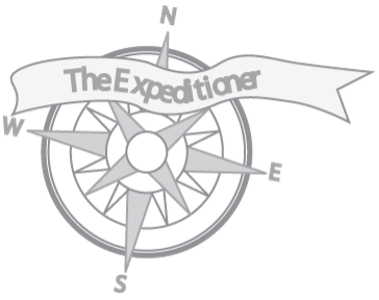
\includegraphics[width=1.97917in,height=\textheight]{Figures/Chapter 1/expeditioner.png}

Alice has found several histories of The Expeditioner from a variety of
eras. Because many expeditions they outfitted were conducted under royal
patronage, it was not uncommon for these histories to refer to British
monarchs. Alice could remember very little about British history, let
alone when various kings and queens reigned. This sounded like another
database problem. She would ask Ned to create a database that recorded
details of each monarch. She thought it also would be useful to record
details of royal succession.

\hypertarget{modeling-a-recursive-one-to-one-relationship}{%
\subsection*{Modeling a recursive one-to-one relationship}\label{modeling-a-recursive-one-to-one-relationship}}
\addcontentsline{toc}{subsection}{Modeling a recursive one-to-one relationship}

The British monarchy can be represented by a simple one-entity model. A
monarch has one direct successor and one direct predecessor. The
sequencing of monarchs can be modeled by a recursive 1:1 relationship,
shown in the following figure.

\emph{A data model illustrating a recursive 1:1 relationship}

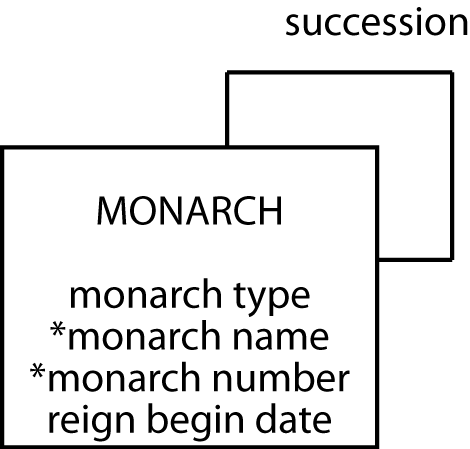
\includegraphics[width=2.45833in,height=\textheight]{Figures/Chapter 6/recursive-1-and-1.png}

\emph{MySQL Workbench version of a recursive 1:1 relationship}

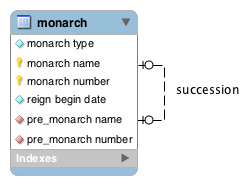
\includegraphics{Figures/Chapter 6/recursive-1-and-1-wb.png}

\hypertarget{mapping-a-recursive-one-to-one-relationship}{%
\subsection*{Mapping a recursive one-to-one relationship}\label{mapping-a-recursive-one-to-one-relationship}}
\addcontentsline{toc}{subsection}{Mapping a recursive one-to-one relationship}

The recursive 1:1 relationship is mapped by adding a foreign key to
\texttt{monarch}. You can add a foreign key to represent either the successor
or predecessor relationship. In this case, for no particular reason, the
preceding relationship is selected. Because each instance of a monarch
is identified by a composite key, two columns are added to \texttt{monarch} for
the foreign key. Data for recent monarchs are shown in the following
table.

\emph{The table monarch}

\begin{longtable}[]{@{}llcllc@{}}
\toprule
montype & monname & monnum & rgnbeg & premonname & premonnum \\
\midrule
\endhead
King & William & IV & 1830/6/26 & & \\
Queen & Victoria & I & 1837/6/20 & William & IV \\
King & Edward & VII & 1901/1/22 & Victoria & I \\
King & George & V & 1910/5/6 & Edward & VII \\
King & Edward & VIII & 1936/1/20 & George & V \\
King & George & VI & 1936/12/11 & Edward & VIII \\
Queen & Elizabeth & II & 1952/02/06 & George & VI \\
\bottomrule
\end{longtable}

The SQL statements to create the table are very straightforward.

\begin{Shaded}
\begin{Highlighting}[]
\KeywordTok{CREATE} \KeywordTok{TABLE}\NormalTok{ monarch (}
\NormalTok{    montype     }\DataTypeTok{CHAR}\NormalTok{(}\DecValTok{5}\NormalTok{) }\KeywordTok{NOT} \KeywordTok{NULL}\NormalTok{,}
\NormalTok{    monname     }\DataTypeTok{VARCHAR}\NormalTok{(}\DecValTok{15}\NormalTok{),}
\NormalTok{    monnum          }\DataTypeTok{VARCHAR}\NormalTok{(}\DecValTok{5}\NormalTok{),}
\NormalTok{    rgnbeg          }\DataTypeTok{DATE}\NormalTok{,}
\NormalTok{    premonname      }\DataTypeTok{VARCHAR}\NormalTok{(}\DecValTok{15}\NormalTok{),}
\NormalTok{    premonnum       }\DataTypeTok{VARCHAR}\NormalTok{(}\DecValTok{5}\NormalTok{),}
    \KeywordTok{PRIMARY} \KeywordTok{KEY}\NormalTok{(monname,monnum),}
    \KeywordTok{CONSTRAINT}\NormalTok{ fk\_monarch }\KeywordTok{FOREIGN} \KeywordTok{KEY}\NormalTok{ (premonname, premonnum)}
        \KeywordTok{REFERENCES}\NormalTok{ monarch(monname, monnum);}
\end{Highlighting}
\end{Shaded}

Because the 1:1 relationship is recursive, you cannot insert Queen
Victoria without first inserting King William IV. What you can do is
first insert King William, without any reference to the preceding
monarch (i.e., a null foreign key). The following code illustrates the
order of record insertion so that the referential integrity constraint
is obeyed.

\begin{Shaded}
\begin{Highlighting}[]
\KeywordTok{INSERT} \KeywordTok{INTO}\NormalTok{ MONARCH (montype,monname, monnum,rgnbeg) }\KeywordTok{VALUES}\NormalTok{ (}\StringTok{\textquotesingle{}King\textquotesingle{}}\NormalTok{,}\StringTok{\textquotesingle{}William\textquotesingle{}}\NormalTok{,}\StringTok{\textquotesingle{}IV\textquotesingle{}}\NormalTok{,}\StringTok{\textquotesingle{}1830{-}06{-}26\textquotesingle{}}\NormalTok{);}
\KeywordTok{INSERT} \KeywordTok{INTO}\NormalTok{ MONARCH }\KeywordTok{VALUES}\NormalTok{ (}\StringTok{\textquotesingle{}Queen\textquotesingle{}}\NormalTok{,}\StringTok{\textquotesingle{}Victoria\textquotesingle{}}\NormalTok{,}\StringTok{\textquotesingle{}I\textquotesingle{}}\NormalTok{,}\StringTok{\textquotesingle{}1837{-}06{-}20\textquotesingle{}}\NormalTok{,}\StringTok{\textquotesingle{}William\textquotesingle{}}\NormalTok{,}\StringTok{\textquotesingle{}IV\textquotesingle{}}\NormalTok{);}
\KeywordTok{INSERT} \KeywordTok{INTO}\NormalTok{ MONARCH }\KeywordTok{VALUES}\NormalTok{ (}\StringTok{\textquotesingle{}King\textquotesingle{}}\NormalTok{,}\StringTok{\textquotesingle{}Edward\textquotesingle{}}\NormalTok{,}\StringTok{\textquotesingle{}VII\textquotesingle{}}\NormalTok{,}\StringTok{\textquotesingle{}1901{-}01{-}22\textquotesingle{}}\NormalTok{,}\StringTok{\textquotesingle{}Victoria\textquotesingle{}}\NormalTok{,}\StringTok{\textquotesingle{}I\textquotesingle{}}\NormalTok{);}
\KeywordTok{INSERT} \KeywordTok{INTO}\NormalTok{ MONARCH }\KeywordTok{VALUES}\NormalTok{ (}\StringTok{\textquotesingle{}King\textquotesingle{}}\NormalTok{,}\StringTok{\textquotesingle{}George\textquotesingle{}}\NormalTok{,}\StringTok{\textquotesingle{}V\textquotesingle{}}\NormalTok{,}\StringTok{\textquotesingle{}1910{-}05{-}06\textquotesingle{}}\NormalTok{,}\StringTok{\textquotesingle{}Edward\textquotesingle{}}\NormalTok{,}\StringTok{\textquotesingle{}VII\textquotesingle{}}\NormalTok{);}
\KeywordTok{INSERT} \KeywordTok{INTO}\NormalTok{ MONARCH }\KeywordTok{VALUES}\NormalTok{ (}\StringTok{\textquotesingle{}King\textquotesingle{}}\NormalTok{,}\StringTok{\textquotesingle{}Edward\textquotesingle{}}\NormalTok{,}\StringTok{\textquotesingle{}VIII\textquotesingle{}}\NormalTok{,}\StringTok{\textquotesingle{}1936{-}01{-}20\textquotesingle{}}\NormalTok{,}\StringTok{\textquotesingle{}George\textquotesingle{}}\NormalTok{,}\StringTok{\textquotesingle{}V\textquotesingle{}}\NormalTok{);}
\KeywordTok{INSERT} \KeywordTok{INTO}\NormalTok{ MONARCH }\KeywordTok{VALUES}\NormalTok{(}\StringTok{\textquotesingle{}King\textquotesingle{}}\NormalTok{,}\StringTok{\textquotesingle{}George\textquotesingle{}}\NormalTok{,}\StringTok{\textquotesingle{}VI\textquotesingle{}}\NormalTok{,}\StringTok{\textquotesingle{}1936{-}12{-}11\textquotesingle{}}\NormalTok{,}\StringTok{\textquotesingle{}Edward\textquotesingle{}}\NormalTok{,}\StringTok{\textquotesingle{}VIII\textquotesingle{}}\NormalTok{);}
\KeywordTok{INSERT} \KeywordTok{INTO}\NormalTok{ MONARCH }\KeywordTok{VALUES}\NormalTok{(}\StringTok{\textquotesingle{}Queen\textquotesingle{}}\NormalTok{,}\StringTok{\textquotesingle{}Elizabeth\textquotesingle{}}\NormalTok{,}\StringTok{\textquotesingle{}II\textquotesingle{}}\NormalTok{,}\StringTok{\textquotesingle{}1952{-}02{-}06\textquotesingle{}}\NormalTok{,}\StringTok{\textquotesingle{}George\textquotesingle{}}\NormalTok{,}\StringTok{\textquotesingle{}VI\textquotesingle{}}\NormalTok{);}
\end{Highlighting}
\end{Shaded}

\begin{quote}
❓\emph{Skill builder}

In a competitive bridge competition, the same pair of players play
together for the entire tournament. Draw a data model to record
details of all the players and the pairs of players.ß
\end{quote}

\hypertarget{querying-a-recursive-one-to-one-relationship}{%
\subsection*{Querying a recursive one-to-one relationship}\label{querying-a-recursive-one-to-one-relationship}}
\addcontentsline{toc}{subsection}{Querying a recursive one-to-one relationship}

Some queries on the monarch table demonstrate querying a recursive 1:1
relationship.

\emph{Who preceded Elizabeth II?}

\begin{Shaded}
\begin{Highlighting}[]
\KeywordTok{SELECT}\NormalTok{ premonname, premonnum }\KeywordTok{FROM}\NormalTok{ monarch}
    \KeywordTok{WHERE}\NormalTok{ monname }\OperatorTok{=} \StringTok{\textquotesingle{}Elizabeth\textquotesingle{}} \KeywordTok{and}\NormalTok{ monnum }\OperatorTok{=} \StringTok{\textquotesingle{}II\textquotesingle{}}\NormalTok{;}
\end{Highlighting}
\end{Shaded}

\begin{table}

\caption{\label{tab:unnamed-chunk-83}1 records}
\centering
\begin{tabular}[t]{l|l}
\hline
premonname & premonnum\\
\hline
George & VI\\
\hline
\end{tabular}
\end{table}

This is simple because all the data are in one row. A more complex query
is:

\emph{Was Elizabeth II's predecessor a king or queen?}

\begin{Shaded}
\begin{Highlighting}[]
\KeywordTok{WITH}
\NormalTok{cur }\KeywordTok{AS}\NormalTok{ (}\KeywordTok{SELECT} \OperatorTok{*} \KeywordTok{FROM}\NormalTok{ monarch), }
\NormalTok{pre }\KeywordTok{AS}\NormalTok{ (}\KeywordTok{SELECT} \OperatorTok{*} \KeywordTok{FROM}\NormalTok{ monarch) }
\KeywordTok{SELECT}\NormalTok{ pre.montype }\KeywordTok{FROM}\NormalTok{ cur }\KeywordTok{JOIN}\NormalTok{  pre}
    \KeywordTok{ON}\NormalTok{ cur.premonname }\OperatorTok{=}\NormalTok{ pre.monname }\KeywordTok{AND}\NormalTok{ cur.premonnum }\OperatorTok{=}\NormalTok{ pre.monnum}
    \KeywordTok{WHERE}\NormalTok{ cur.monname }\OperatorTok{=} \StringTok{\textquotesingle{}Elizabeth\textquotesingle{}}
    \KeywordTok{AND}\NormalTok{ cur.monnum }\OperatorTok{=} \StringTok{\textquotesingle{}II\textquotesingle{}}\NormalTok{;}
\end{Highlighting}
\end{Shaded}

\begin{table}

\caption{\label{tab:unnamed-chunk-84}1 records}
\centering
\begin{tabular}[t]{l}
\hline
montype\\
\hline
King\\
\hline
\end{tabular}
\end{table}

Notice in the preceding query how to specify the ON clause when you have
a composite key.

This is very similar to the query to find the salary of Nancy's boss.
The \texttt{monarch} table is joined with itself to create a row that contains
all the details to answer the query.

\emph{List the kings and queens of England in ascending chronological order.}

\begin{Shaded}
\begin{Highlighting}[]
\KeywordTok{SELECT}\NormalTok{ montype, monname, monnum, rgnbeg}
    \KeywordTok{FROM}\NormalTok{ monarch }\KeywordTok{ORDER} \KeywordTok{BY}\NormalTok{ rgnbeg;}
\end{Highlighting}
\end{Shaded}

\begin{table}

\caption{\label{tab:unnamed-chunk-85}7 records}
\centering
\begin{tabular}[t]{l|l|l|l}
\hline
montype & monname & monnum & rgnbeg\\
\hline
King & William & IV & 1830-06-26\\
\hline
Queen & Victoria & I & 1837-06-20\\
\hline
King & Edward & VII & 1901-01-22\\
\hline
King & George & V & 1910-05-06\\
\hline
King & Edward & VIII & 1936-01-20\\
\hline
King & George & VI & 1936-12-11\\
\hline
Queen & Elizabeth & II & 1952-02-06\\
\hline
\end{tabular}
\end{table}

This is a simple query because \texttt{rgnbeg} is like a ranking column. It
would not be enough to store just the year in \texttt{rgnbeg}, because two
kings started their reigns in 1936; hence, the full date is required.

\begin{quote}
❓\emph{Skill builder}

Who succeeded Queen Victoria?
\end{quote}

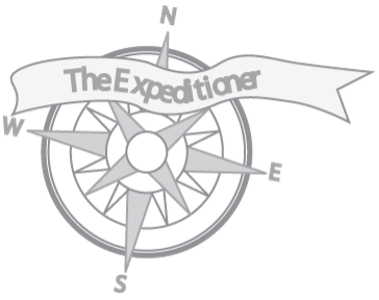
\includegraphics[width=1.97917in,height=\textheight]{Figures/Chapter 1/expeditioner.png}

Of course, Alice soon had another project for Ned. The Expeditioner
keeps a wide range of products that are sometimes assembled into kits to
make other products. For example, the animal photography kit is made up
of eight items that The Expeditioner also sells separately. In addition,
some kits became part of much larger kits. The animal photography kit is
included as one of 45 items in the East African Safari package. All of
the various items are considered products, and each has its own product
code. Ned was now required to create a product database that would keep
track of all the items in The Expeditioner's stock.

\hypertarget{modeling-a-recursive-many-to-many-relationship}{%
\subsection*{Modeling a recursive many-to-many relationship}\label{modeling-a-recursive-many-to-many-relationship}}
\addcontentsline{toc}{subsection}{Modeling a recursive many-to-many relationship}

The assembly of products to create other products is very common in
business. Manufacturing even has a special term to describe it: a bill
of materials. The data model is relatively simple once you realize that
a product can appear as part of many other products and can be composed
of many other products; that is, we have a recursive many-to-many (m:m)
relationship for product. As usual, we turn an m:m relationship into two
one-to-many (1:m) relationships. Thus, we get the data model displayed
in the following figure.

\emph{A data model illustrating a recursive m:m relationship}

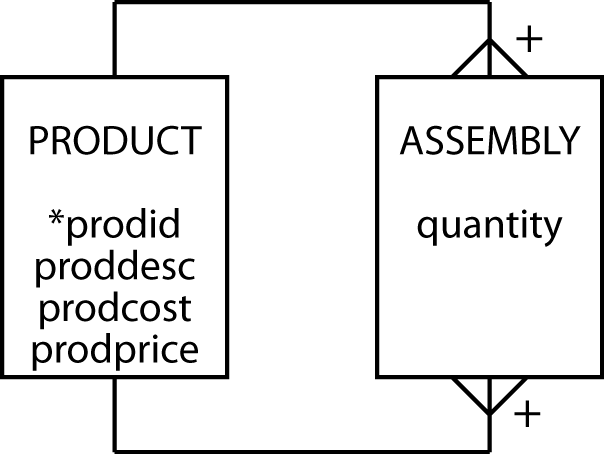
\includegraphics[width=3.14583in,height=\textheight]{Figures/Chapter 6/recursive-m-and-m.png}

\emph{MySQL Workbench version of a recursive m:m relationship}

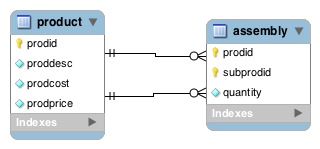
\includegraphics{Figures/Chapter 6/recursive-m-and-m-wb.png}

\emph{Tables product and assembly}

\begin{longtable}[]{@{}rlrr@{}}
\toprule
\underline{prodid} & proddesc & prodcost & prodprice \\
\midrule
\endhead
1000 & Animal photography kit & & 725 \\
101 & Camera & 150 & 300 \\
102 & Camera case & 10 & 15 \\
103 & 70-210 zoom lens & 125 & 200 \\
104 & 28-85 zoom lens & 115 & 185 \\
105 & Photographer's vest & 25 & 40 \\
106 & Lens cleaning cloth & 1 & 1.25 \\
107 & Tripod & 35 & 45 \\
108 & 16 GB SDHC memory card & 30 & 37 \\
\bottomrule
\end{longtable}

\begin{longtable}[]{@{}rrr@{}}
\toprule
quantity & \underline{\emph{prodid}} & \underline{\emph{subprodid}} \\
\midrule
\endhead
1 & 1000 & 101 \\
1 & 1000 & 102 \\
1 & 1000 & 103 \\
1 & 1000 & 104 \\
1 & 1000 & 105 \\
2 & 1000 & 106 \\
1 & 1000 & 107 \\
10 & 1000 & 108 \\
\bottomrule
\end{longtable}

\hypertarget{mapping-a-recursive-many-to-many-relationship}{%
\subsection*{Mapping a recursive many-to-many relationship}\label{mapping-a-recursive-many-to-many-relationship}}
\addcontentsline{toc}{subsection}{Mapping a recursive many-to-many relationship}

Mapping follows the same procedure described previously, producing the
two tables shown below. The SQL statements to create the tables are
shown next. Observe that \texttt{assembly} has a composite key, and there are
two foreign key constraints.

\begin{Shaded}
\begin{Highlighting}[]
\KeywordTok{CREATE} \KeywordTok{TABLE}\NormalTok{ product (}
\NormalTok{    prodid          }\DataTypeTok{INTEGER}\NormalTok{,}
\NormalTok{    proddesc        }\DataTypeTok{VARCHAR}\NormalTok{(}\DecValTok{30}\NormalTok{),}
\NormalTok{    prodcost        }\DataTypeTok{DECIMAL}\NormalTok{(}\DecValTok{9}\NormalTok{,}\DecValTok{2}\NormalTok{),}
\NormalTok{    prodprice       }\DataTypeTok{DECIMAL}\NormalTok{(}\DecValTok{9}\NormalTok{,}\DecValTok{2}\NormalTok{),}
        \KeywordTok{PRIMARY} \KeywordTok{KEY}\NormalTok{(prodid));}
\end{Highlighting}
\end{Shaded}

\begin{Shaded}
\begin{Highlighting}[]
\KeywordTok{CREATE} \KeywordTok{TABLE}\NormalTok{ assembly (}
\NormalTok{    quantity        }\DataTypeTok{INTEGER} \KeywordTok{NOT} \KeywordTok{NULL}\NormalTok{,}
\NormalTok{    prodid          }\DataTypeTok{INTEGER}\NormalTok{,}
\NormalTok{    subprodid       }\DataTypeTok{INTEGER}\NormalTok{,}
        \KeywordTok{PRIMARY} \KeywordTok{KEY}\NormalTok{(prodid, subprodid),}
        \KeywordTok{CONSTRAINT}\NormalTok{ fk\_assembly\_product }\KeywordTok{FOREIGN} \KeywordTok{KEY}\NormalTok{(prodid)}
            \KeywordTok{REFERENCES}\NormalTok{ product(prodid),}
        \KeywordTok{CONSTRAINT}\NormalTok{ fk\_assembly\_subproduct }\KeywordTok{FOREIGN} \KeywordTok{KEY}\NormalTok{(subprodid)}
            \KeywordTok{REFERENCES}\NormalTok{ product(prodid));}
\end{Highlighting}
\end{Shaded}

\begin{quote}
❓\emph{Skill builder}

An army is broken up into many administrative units (e.g., army,
brigade, platoon). A unit can contain many other units (e.g., a
regiment contains two or more battalions), and a unit can be part of a
larger unit (e.g., a squad is a member of a platoon). Draw a data
model for this situation.\\
\#\# Querying a recursive many-to-many relationship \{-\}
\end{quote}

\emph{List the product identifier of each component of the animal photography
kit.}

\begin{Shaded}
\begin{Highlighting}[]
\KeywordTok{SELECT}\NormalTok{ subprodid }\KeywordTok{FROM}\NormalTok{ product }\KeywordTok{JOIN}\NormalTok{ assembly}
    \KeywordTok{ON}\NormalTok{ product.prodid }\OperatorTok{=}\NormalTok{ assembly.prodid}
    \KeywordTok{WHERE}\NormalTok{ proddesc }\OperatorTok{=} \StringTok{\textquotesingle{}Animal photography kit\textquotesingle{}}\NormalTok{;}
\end{Highlighting}
\end{Shaded}

\begin{table}

\caption{\label{tab:unnamed-chunk-88}8 records}
\centering
\begin{tabular}[t]{l}
\hline
subprodid\\
\hline
101\\
\hline
102\\
\hline
103\\
\hline
104\\
\hline
105\\
\hline
106\\
\hline
107\\
\hline
108\\
\hline
\end{tabular}
\end{table}

Why are the values for \texttt{subprodid} listed in no apparent order?
Remember, there is no implied ordering of rows in a table, and it is
quite possible, as this example illustrates, for the rows to have what
appears to be an unusual ordering. If you want to order rows, use the
ORDER BY clause.

\emph{List the product description and cost of each component of the animal
photography kit.}

\begin{Shaded}
\begin{Highlighting}[]
\KeywordTok{SELECT}\NormalTok{ proddesc, prodcost }\KeywordTok{FROM}\NormalTok{ product}
    \KeywordTok{WHERE}\NormalTok{ prodid }\KeywordTok{IN}
\NormalTok{        (}\KeywordTok{SELECT}\NormalTok{ subprodid }\KeywordTok{FROM}\NormalTok{ product }\KeywordTok{JOIN}\NormalTok{ assembly}
                \KeywordTok{ON}\NormalTok{ product.prodid }\OperatorTok{=}\NormalTok{ assembly.prodid}
                \KeywordTok{WHERE}\NormalTok{ proddesc }\OperatorTok{=} \StringTok{\textquotesingle{}Animal photography kit\textquotesingle{}}\NormalTok{);}
\end{Highlighting}
\end{Shaded}

In this case, first determine the \texttt{prodid} of those products in the
animal photography kit (the inner query), and then report the
description of these products. Alternatively, a three-way join can be
done using two copies of \texttt{product}.

\begin{Shaded}
\begin{Highlighting}[]
\KeywordTok{WITH}
\NormalTok{a }\KeywordTok{AS}\NormalTok{ (}\KeywordTok{SELECT} \OperatorTok{*} \KeywordTok{FROM}\NormalTok{ product), }
\NormalTok{b }\KeywordTok{AS}\NormalTok{ (}\KeywordTok{SELECT} \OperatorTok{*} \KeywordTok{FROM}\NormalTok{ product) }
\KeywordTok{SELECT}\NormalTok{ b.proddesc, b.prodcost }\KeywordTok{FROM}\NormalTok{ a }\KeywordTok{JOIN}\NormalTok{ assembly}
        \KeywordTok{ON}\NormalTok{ a.prodid }\OperatorTok{=}\NormalTok{ assembly.prodid}
        \KeywordTok{JOIN}\NormalTok{ b}
        \KeywordTok{ON}\NormalTok{ assembly.subprodid }\OperatorTok{=}\NormalTok{ b.prodid}
        \KeywordTok{WHERE}\NormalTok{ a.proddesc }\OperatorTok{=} \StringTok{\textquotesingle{}Animal photography kit\textquotesingle{}}\NormalTok{;}
\end{Highlighting}
\end{Shaded}

\begin{table}

\caption{\label{tab:unnamed-chunk-90}8 records}
\centering
\begin{tabular}[t]{l|r}
\hline
proddesc & prodcost\\
\hline
35mm camera & 150.00\\
\hline
Camera case & 10.00\\
\hline
70-210 zoom lens & 125.00\\
\hline
28-85 zoom lens & 115.00\\
\hline
Photographers vest & 25.00\\
\hline
Lens cleaning cloth & 1.00\\
\hline
Tripod & 35.00\\
\hline
24/100 ASA 35mm color neg film & 0.85\\
\hline
\end{tabular}
\end{table}

\begin{quote}
❓\emph{Skill builder}

How many lens cleaning cloths are there in the animal photography kit?
\end{quote}

\hypertarget{summary-5}{%
\subsection*{Summary}\label{summary-5}}
\addcontentsline{toc}{subsection}{Summary}

Relationships can be one-to-one and recursive. A recursive relationship
is within a single entity rather than between entities. Recursive
relationships are mapped to the relational model in the same way as
other relationships. A self-referential foreign key constraint permits a
foreign key reference to a key within the same table. Resolution of
queries involving recursive relationships often requires a table to be
joined with itself. Recursive many-to-many relationships occur in
business in the form of a bill of materials.

\hypertarget{key-terms-and-concepts-3}{%
\subsection*{Key terms and concepts}\label{key-terms-and-concepts-3}}
\addcontentsline{toc}{subsection}{Key terms and concepts}

\begin{longtable}[]{@{}ll@{}}
\toprule
& \\
\midrule
\endhead
JOIN & Relationship \\
One-to-many (1:m) relationship & Relationship descriptor \\
One-to-one (1:1) relationship & Self-join \\
Recursive 1:1 relationship & Self-referential foreign key \\
Recursive 1:m relationship & Theta-join \\
Recursive m:m relationship & Update anomalies \\
Recursive relationship & Views \\
Referential integrity & Virtual table \\
\bottomrule
\end{longtable}

\hypertarget{exercise}{%
\subsection*{Exercise}\label{exercise}}
\addcontentsline{toc}{subsection}{Exercise}

\begin{enumerate}
\def\labelenumi{\arabic{enumi}.}
\item
  Draw data models for the following two problems:

  \begin{enumerate}
  \def\labelenumii{\alph{enumii}.}
  \item
    \begin{enumerate}
    \def\labelenumiii{(\roman{enumiii})}
    \item
      A dairy farmer, who is also a part-time cartoonist, has
      several herds of cows. He has assigned each cow to a
      particular herd. In each herd, the farmer has one cow that
      is his favorite---often that cow is featured in a cartoon.\\
    \item
      A few malcontents in each herd, mainly those who feel they
      should have appeared in the cartoon, disagree with the
      farmer's choice of a favorite cow, whom they disparagingly
      refer to as the sacred cow. As a result, each herd now has
      elected a herd leader.
    \end{enumerate}
  \item
    The originator of a pyramid marketing scheme has a system for
    selling ethnic jewelry. The pyramid has three levels---gold,
    silver, and bronze. New associates join the pyramid at the
    bronze level. They contribute 30 percent of the revenue of their
    sales of jewelry to the silver chief in charge of their clan. In
    turn, silver chiefs contribute 30 percent of what they receive
    from bronze associates to the gold master in command of their
    tribe. Finally, gold masters pass on 30 percent of what they
    receive to the originator of the scheme.
  \item
    The legion, the basic combat unit of the ancient Roman army,
    contained 3,000 to 6,000 men, consisting primarily of heavy
    infantry (hoplites), supported by light infantry (velites), and
    sometimes by cavalry. The hoplites were drawn up in three lines.
    The hastati (youngest men) were in the first, the principes
    (seasoned troops) in the second, and the triarii (oldest men)
    behind them, reinforced by velites. Each line was divided into
    10 maniples, consisting of two centuries (60 to 80 men per
    century) each. Each legion had a commander, and a century was
    commanded by a centurion. Julius Caesar, through one of his
    Californian channelers, has asked you to design a database to
    maintain details of soldiers. Of course, Julius is a little
    forgetful at times, and he has not supplied the titles of the
    officers who command maniples, lines, and hoplites, but he
    expects that you can handle this lack of fine detail.
  \item
    A travel agency is frequently asked questions about tourist
    destinations. For example, customers want to know details of the
    climate for a particular month, the population of the city, and
    other geographic facts. Sometimes they request the flying time
    and distance between two cities. The manager has asked you to
    create a database to maintain these facts.
  \item
    The Center for the Study of World Trade keeps track of trade
    treaties between nations. For each treaty, it records details of
    the countries signing the treaty and where and when it was
    signed.
  \item
    Design a database to store details about U.S. presidents and
    their terms in office. Also, record details of their date and
    place of birth, gender, and political party affiliation (e.g.,
    Caluthumpian Progress Party). You are required to record the
    sequence of presidents so that the predecessor and successor of
    any president can be identified. How will you model the case of
    Grover Cleveland, who served nonconsecutive terms as president?
    Is it feasible that political party affiliation may change? If
    so, how will you handle it?
  \item
    The IS department of a large organization makes extensive use of
    software modules. New applications are built, where possible,
    from existing modules. Software modules can also contain other
    modules. The IS manager realizes that she now needs a database
    to keep track of which modules are used in which applications or
    other modules. (Hint: It is helpful to think of an application
    as a module.)
  \item
    Data modeling is finally getting to you. Last night you dreamed
    you were asked by Noah to design a database to store data about
    the animals on the ark. All you can remember from Sunday school
    is the bit about the animals entering the ark two-by-two, so you
    thought you should check the real thing.\\
    Take with you seven pairs of every kind of clean animal, a male
    and its mate, and two of every kind of unclean animal, a male
    and its mate, and also seven pair of every kind of bird, male
    and female. Genesis 7:2\\
    Next time Noah disturbs your sleep, you want to be ready. So,
    draw a data model and make certain you record the two-by-two
    relationship.
  \end{enumerate}
\item
  Write SQL to answer the following queries using the DEPT and EMP
  tables described in this chapter:

  \begin{enumerate}
  \def\labelenumii{\alph{enumii}.}
  \item
    Find the departments where all the employees earn less than
    their boss.
  \item
    Find the names of employees who are in the same department as
    their boss (as an employee).
  \item
    List the departments having an average salary greater than
    \$25,000.
  \item
    List the departments where the average salary of the employees,
    excluding the boss, is greater than \$25,000.
  \item
    List the names and manager of the employees of the Marketing
    department who have a salary greater than \$25,000.
  \item
    List the names of the employees who earn more than any employee
    in the Marketing department.
  \end{enumerate}
\item
  Write SQL to answer the following queries using the monarch table
  described in this chapter:

  \begin{enumerate}
  \def\labelenumii{\alph{enumii}.}
  \item
    Who succeeded Victoria I?
  \item
    How many days did Victoria I reign?
  \item
    How many kings are there in the table?
  \item
    Which monarch had the shortest reign?
  \end{enumerate}
\item
  Write SQL to answer the following queries using the product and
  assembly tables:

  \begin{enumerate}
  \def\labelenumii{\alph{enumii}.}
  \item
    How many different items are there in the animal photography
    kit?
  \item
    What is the most expensive item in the animal photography kit?
  \item
    What is the total cost of the components of the animal
    photography kit?
  \item
    Compute the total quantity for each of the items required to
    assemble 15 animal photography kits.
  \end{enumerate}
\end{enumerate}

\hypertarget{data-modeling}{%
\section{Data Modeling}\label{data-modeling}}

\begin{quote}
\emph{Man is a knot, a web, a mesh into which relationships are tied. Only
those relationships matter.}

Antoine de Saint-Exupéry in \emph{Flight to Arras}
\end{quote}

\hypertarget{learning-objectives-6}{%
\subsubsection*{Learning objectives}\label{learning-objectives-6}}
\addcontentsline{toc}{subsubsection}{Learning objectives}

Students completing this chapter will be able to create a well-formed,
high-fidelity data model.

\hypertarget{modeling}{%
\subsection*{Modeling}\label{modeling}}
\addcontentsline{toc}{subsection}{Modeling}

Modeling is widely used within business to learn about organizational
problems and design solutions. To understand where data modeling fits
within the broader context, it is useful to review the full range of
modeling activities. The types of modeling methods follow the 5W-H model
of journalism.\footnote{~Roberto Franzosi, ``On Quantitative Narrative
  Analysis,'' in Varieties of Narrative Analysis, ed.~James A. Holstein
  and Jaber F. Gubrium (SAGE Publications, Inc., 2012), 75--96.}

\emph{A broad perspective on modeling}

\begin{longtable}[]{@{}lllll@{}}
\toprule
& & \textbf{Scope} & \textbf{Model} & \textbf{Technology} \\
\midrule
\endhead
\textbf{Motivation} & Why & Goals & Business plan canvas & Groupware \\
\textbf{People} & Who & Business units & Organization chart & System interface \\
\textbf{Time} & When & Key events & PERT chart & Scheduling \\
\textbf{Data} & What & Key entities & Data model & Relational database \\
\textbf{Network} & Where & Locations & Logistics network & System architecture \\
\textbf{Function} & How & Key processes & Process model & Application software \\
\bottomrule
\end{longtable}

Modeling occurs at multiple levels. At the highest level, an
organization needs to determine the scope of its business by identifying
the major elements of its environment, such as its goals, business
units, where it operates, and critical events, entities, and processes.
At the top level, textual models are frequently used. For example, an
organization might list its major goals and business processes. A map
will be typically used to display where the business operates.

Once senior managers have clarified the scope of a business, models can
be constructed for each of the major elements. Goals will be converted
into a business plan, business units will be shown on an organizational
chart, and so on. The key elements, from an IS perspective, are data and
process modeling, which are typically covered in the core courses of an
IS program.

Technology, the final stage, converts models into operational systems to
support the organization. Many organizations rely extensively on e-mail
and Web technology for communicating business decisions. People connect
to systems through an interface, such as a Web browser. Ensuring that
events occur at the right time is managed by scheduling software. This
could be implemented with operating system procedures that schedule the
execution of applications. In some database management systems (DBMSs),
triggers can be established. A \textbf{trigger} is a database procedure that
is automatically executed when some event is recognized. For example,
U.S. banks are required to report all deposits exceeding USD 10,000, and
a trigger could be coded for this event.

Data models are typically converted into relational databases, and
process models become computer programs. Thus, you can see that data
modeling is one element of a comprehensive modeling activity that is
often required to design business systems. When a business undergoes a
major change, such as a reengineering project, many dimensions can be
altered, and it may be appropriate to rethink many elements of the
business, starting with its goals. Because such major change is very
disruptive and costly, it occurs less frequently. It is more likely that
data modeling is conducted as a stand-alone activity or part of process
modeling to create a new business application.

\hypertarget{data-modeling-1}{%
\subsection*{Data modeling}\label{data-modeling-1}}
\addcontentsline{toc}{subsection}{Data modeling}

You were introduced to the basic building blocks of data modeling in the
earlier chapters of this section. Now it is time to learn how to
assemble blocks to build a data model. Data modeling is a method for
determining what data and relationships should be stored in the
database. It is also a way of communicating a database design.

The goal of data modeling is to identify the facts that must be stored
in a database. A data model is not concerned with how the data will be
stored. This is the concern of those who implement the database. A data
model is not concerned with how the data will be processed. This is the
province of process modeling. The goal is to create a data model that is
an accurate representation of data needs and real-world data
relationships.

Building a data model is a partnership between a client, a
representative of the eventual owners of the database, and a designer.
Of course, there can be a team of clients and designers. For simplicity,
we assume there is one client and one designer.

Drawing a data model is an iterative process of trial and revision. A
data model is a working document that will change as you learn more
about the client's needs and world. Your early versions are likely to be
quite different from the final product. Use a product such as MySQL
Workbench for drawing and revising a data model.

\hypertarget{the-building-blocks}{%
\subsection*{The building blocks}\label{the-building-blocks}}
\addcontentsline{toc}{subsection}{The building blocks}

The purpose of a database is to store data about things, which can
include facts (e.g., an exchange rate), plans (e.g., scheduled
production of two-person tents for June), estimates (e.g., forecast of
demand for smart phones), and a variety of other data. A data model
describes these things and their relationships with other things using
four components: entity, attribute, relationship, and identifier.

\hypertarget{entity}{%
\subsubsection*{Entity}\label{entity}}
\addcontentsline{toc}{subsubsection}{Entity}

The entity is the basic building block of a data model. an entity is a
thing about which data should be stored, something we need to describe.
Each entity in a data model has a unique name that we write in singular
form. Why singular? Because we want to emphasize that an entity
describes an instance of a thing. Thus, we previously used the word
SHARE to define an entity because it describes each instance of a share
rather than shares in general.

We have already introduced the convention that an entity is represented
by a rectangle, and the name of the entity is shown in uppercase
letters, as follows.

\emph{The entity SHARE}


\includegraphics[width=1.58333in,height=\textheight]{Figures/Chapter 3/share.png}

A large data model might contain over a 1,000 entities. A database can
easily contain hundreds of millions of instances (rows) for any one
entity (table). Imagine the number of instances in a national tax
department's database.

How do you begin to identify entities? One approach is to underline any
\emph{nouns} in the system proposal or provided documentation. Most nouns are
possible entities, and underlining ensures that you do not overlook any
potential entities. Start by selecting an entity that seems central to
the problem. If you were designing a student database, you might start
with the student. Once you have picked a central entity, describe it.
Then move to the others.

\hypertarget{attribute}{%
\subsubsection*{Attribute}\label{attribute}}
\addcontentsline{toc}{subsubsection}{Attribute}

An attribute describes an entity. When an entity has been identified,
the next step is to determine its attributes, that is, the data that
should be kept to describe fully the entity. An attribute name is
singular and unique within the data model. You may need to use a
modifier to make an attribute name unique (e.g., ``hire date'' and ``sale
date'' rather than just ``date'').

Our convention is that the name of an attribute is recorded in lowercase
letters within the entity rectangle. The following figure illustrates
that SHARE has attributes \emph{share code, share name, share price, share
quantity, share dividend,} and \emph{share PE}. Notice the frequent use of
the modifier ``share''. It is possible that other entities in the database
might also have a price and quantity, so we use a modifier to create
unique attribute names. Note also that \emph{share cod}e is the identifier.

\emph{The entity SHARE with its attributes}

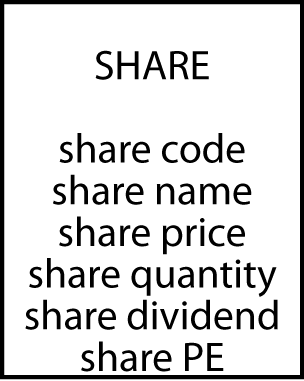
\includegraphics[width=1.58333in,height=\textheight]{Figures/Chapter 3/share with attributes.png}

Defining attributes generally takes considerable discussion with the
client. You should include any attribute that is likely to be required
for present or future decision making, but don't get carried away. Avoid
storing unnecessary data. For example, to describe the entity STUDENT
you usually record date of birth, but it is unlikely that you would
store height. If you were describing an entity PATIENT, on the other
hand, it might be necessary to record height, because that is sometimes
relevant to medical decision making.

An attribute has a single value, which may be null. Multiple values are
not allowed. If you need to store multiple values, it is a signal that
you have a one-to-many (1:m) relationship and need to define another
entity.

\hypertarget{relationship}{%
\subsubsection*{Relationship}\label{relationship}}
\addcontentsline{toc}{subsubsection}{Relationship}

Entities are related to other entities. If there were no relationships
between entities, there would be no need for a data model and no need
for a relational database. A simple, flat file (a single-entity
database) would be sufficient. A relationship is binary. It describes a
linkage between two entities and is represented by a line between them.

Because a relationship is binary, strictly speaking it has two
relationship descriptors, one for each entity. Each relationship
descriptor has a degree stating how many instances of the other entity
may be related to each instance of the described entity. Consider the
entities STOCK and NATION and their 1:m relationship (see the following
figure). We have two relationship descriptors: \emph{stocks of nation} for
NATION and \emph{nation of stock} for STOCK. The relationship descriptor
\emph{stocks of nation} has a degree of m because a nation may have zero or
more listed stocks. The relationship descriptor \emph{nation of stock} has a
degree of 1 because a stock is listed in at most one nation. To reduce
data model clutter, where necessary for clarification, we will use a
single label for the pair of relationship descriptors. Experience shows
this approach captures the meaning of the relationship and improves
readability.

\emph{A 1:m relationship between STOCK and NATION}

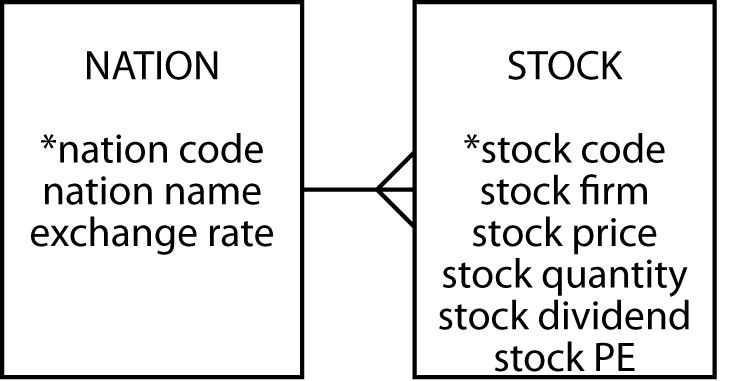
\includegraphics[width=3.89583in,height=\textheight]{Figures/Chapter 4/nation-stock.png}

Because the meaning of relationships frequently can be inferred, there
is no need to label every one; however, each additional relationship
between two entities should be labeled to clarify meaning. Also, it is a
good idea to label one-to-one (1:1) relationships, because the meaning
of the relationship is not always obvious.

Consider the fragment in the following figure. The descriptors of the
1:m relationship can be inferred as a firm has employees and an employee
belongs to a firm. the 1:1 relationship is clarified by labeling the 1:1
relationship as firm's boss.

\emph{Relationship labeling}

\includegraphics{Figures/Chapter 7/relationship labeling.png}

\hypertarget{identifier}{%
\subsubsection*{Identifier}\label{identifier}}
\addcontentsline{toc}{subsubsection}{Identifier}

An identifier uniquely distinguishes an instance of an entity. An
identifier can be one or more attributes and may include the identifier
of a related entity. When a related entity's identifier is part of an
identifier, a plus sign is placed on the line closest to the entity
being identified. In the following figure, an instance of the entity
LINEITEM is identified by the composite of \emph{lineno} and \emph{saleno}, the
identifier of SALE. The value \emph{lineno} does not uniquely identify an
instance of LINEITEM, because it is simply a number that appears on the
sales form. Thus, the identifier must include \emph{saleno} (the identifier
of SALE). So, any instance of LINEITEM is uniquely identified by the
composite \emph{saleno} and \emph{lineno}.

\emph{A related entity's identifier as part of the identifier}

\includegraphics[width=5.84375in,height=\textheight]{Figures/Chapter 5/sale-item.png}

Occasionally, there will be several possible identifiers, and these are
each given a different symbol. Our convention is to prefix an identifier
with an asterisk (*). If there are multiple identifiers, use other
symbols such as \#, !, or \&. Be careful: If you have too many possible
identifiers, your model will look like comic book swearing. In most
cases, you will have only one identifier.

No part of an identifier can be null. If this were permitted, there
would be no guarantee that the other parts of the identifier were
sufficiently unique to distinguish all instances in the database.

\hypertarget{data-model-quality}{%
\subsection*{Data model quality}\label{data-model-quality}}
\addcontentsline{toc}{subsection}{Data model quality}

There are two criteria for judging the quality of a data model. It must
be well-formed and have high fidelity.

\hypertarget{a-well-formed-data-model}{%
\subsubsection*{A well-formed data model}\label{a-well-formed-data-model}}
\addcontentsline{toc}{subsubsection}{A well-formed data model}

A well-formed data model clearly communicates information to the client.
Being well-formed means the construction rules have been obeyed. There
is no ambiguity; all entities are named, and all entities have
identifiers. If identifiers are missing, the client may make incorrect
inferences about the data model. All relationships are recorded using
the proper notation and labeled whenever there is a possibility of
confusion.

\emph{Characteristics of a well-formed data model}

\begin{longtable}[]{@{}l@{}}
\toprule
All construction rules are obeyed. \\
\midrule
\endhead
There is no ambiguity. \\
All entities are named. \\
Every entity has an identifier. \\
All relationships are represented, using the correct notation. \\
Relationships are labeled to avoid misunderstanding. \\
All attributes of each entity are listed. \\
All attribute names are meaningful and unique. \\
\bottomrule
\end{longtable}

All the attributes of an entity are listed because missing attributes
create two types of problems. \emph{First\textbf{,}} it is unclear what data will
be stored about each instance. \emph{Second}, the data model may be missing
some relationships. Attributes that can have multiple values become
entities. It is only by listing all of an entity's attributes during
data modeling that these additional entities are recognized.

In a well-formed data model, all attribute names are meaningful and
unique. The names of entities, identifiers, attributes, and
relationships must be meaningful to the client because they are describe
the client's world. Indeed, in nearly all cases they are the client's
everyday names. Take care in selecting words because they are critical
to communicating meaning. The acid test for comprehension is to get the
client to read the data model to other potential users. Names need to be
unique to avoid confusion.

\hypertarget{a-high-fidelity-image}{%
\subsubsection*{A high-fidelity image}\label{a-high-fidelity-image}}
\addcontentsline{toc}{subsubsection}{A high-fidelity image}

Music lovers aspire to own a high-fidelity stereo system---one that
faithfully reproduces the original performance with minimal or no
distortion. A data model is a high-fidelity image when it faithfully
describes the world it is supposed to represent. All relationships are
recorded and are of the correct degree. There are no compromises or
distortions. If the real-world relationship is many-to-many (m:m), then
so is the relationship shown in the data model. a well-formed,
high-fidelity data model is complete, understandable, accurate, and
syntactically correct.

\hypertarget{quality-improvement}{%
\subsection*{Quality improvement}\label{quality-improvement}}
\addcontentsline{toc}{subsection}{Quality improvement}

A data model is an evolving representation. Each change should be an
incremental improvement in quality. Occasionally, you will find a major
quality problem at the data model's core and have to change the model
considerably.

\hypertarget{detail-and-context}{%
\subsubsection*{Detail and context}\label{detail-and-context}}
\addcontentsline{toc}{subsubsection}{Detail and context}

The quality of a data model can be determined only by understanding the
context in which it will be used. Consider the data model (see the
following figure) used in Chapter 4 to discuss the 1:m relationship.
This fragment says a nation has many stocks. Is that really what we want
to represent? Stocks are listed on a stock exchange, and a nation may
have several stock exchanges. For example, the U.S. has the New York
Stock Exchange and NASDAQ. Furthermore, some foreign stocks are listed
on the New York Stock Exchange. If this is the world we have to
describe, the data model is likely to differ from that shown in the
figure. Try drawing the revised data model.

\emph{A 1:m relationship between STOCK and NATION}

\includegraphics[width=3.89583in,height=\textheight]{Figures/Chapter 4/nation-stock.png}

As you can see, the data model in the following figure is quite
different from the initial data model of preceding figure. Which one is
better? They both can be valid models; it just depends on the world you
are trying to represent and possible future queries. In the first case,
the purpose was to determine the value of a portfolio. There was no
interest in on which exchange stocks were listed or their home exchange.
So the first model has high fidelity for the described situation.

The second data model would be appropriate if the client needed to know
the home exchange of stocks and their price on the various exchanges
where they were listed. The second data model is an improvement on the
first if it incorporates the additional facts and relationships
required. If it does not, then the additional detail is not worth the
extra cost.

\emph{Revised NATION-STOCK data}

\includegraphics{Figures/Chapter 7/revised NATION-STOCK.png}

\hypertarget{a-lesson-in-pure-geography}{%
\subsubsection*{A lesson in pure geography}\label{a-lesson-in-pure-geography}}
\addcontentsline{toc}{subsubsection}{A lesson in pure geography}

A data model must be an accurate representation of the world you want to
model. The data model must account for all the exceptions---there should
be no impurities. Let's say you want to establish a database to store
details of the world's cities. You might start with the data model
depicted in the following figure.

\emph{A world's cities data model}

\includegraphics[width=5.625in,height=\textheight]{Figures/Chapter 7/geography.png}

Before looking more closely at the data model, let's clarify the meaning
of \emph{unittype}. Because most countries are divided into administrative
units that are variously called states, provinces, territories, and so
forth, \emph{unittype} indicates the type of administrative unit (e.g.,
state). How many errors can you find in the initial data model?

Problems and solutions for the initial world's cities data model

\begin{longtable}[]{@{}
  >{\raggedright\arraybackslash}p{(\columnwidth - 4\tabcolsep) * \real{0.17}}
  >{\raggedright\arraybackslash}p{(\columnwidth - 4\tabcolsep) * \real{0.40}}
  >{\raggedright\arraybackslash}p{(\columnwidth - 4\tabcolsep) * \real{0.40}}@{}}
\toprule
& Problem & Solution \\
\midrule
\endhead
1 & City names are not unique.
There is an Athens in
Greece and the U.S. has an
Athens in Georgia,
Alabama, Ohio,
Pennsylvania, Tennessee,
and Texas. & To identify a city
uniquely, you need to
specify its administrative
unit and country. Add a
plus sign to the crow's
feet between CITY and
ADMIN UNIT and between
ADMIN UNIT and NATION. \\
2 & Administrative unit names
are not necessarily
unique. There used to be a
Georgia in the old
U.S.S.R., and there is a
Georgia in the U.S. There
is no guarantee that
administrative unit names
will always be unique. & To identify an
administrative unit
uniquely, you also need to
know the country in which
it is found. Add a plus
sign to the crow's foot
between ADMIN UNIT and
NATION. \\
3 & There is an unlabeled 1:1
relationship between CITY
and ADMIN UNIT and CITY
and NATION. What do these
mean? They are supposed to
indicate that an
administrative unit has a
capital, and a nation has
a capital. & Label relationships (e.g.,
national capital city). \\
4 & The assumption is that a
nation has only one
capital, but there are
exceptions. South Africa
has three capitals: Cape
Town (legislative),
Pretoria (administrative),
and Bloemfontein
(judicial). You need only
one exception to lower the
fidelity of a data model
significantly. & Change the relationship
between NATION and CITY to
1:m. Add an attribute
natcaptype to CITY to
distinguish between types
of capitals. \\
5 & The assumption is that an
administrative unit has
only one capital, but
there are exceptions. At
one point, Chandigarh was
the capital of two Indian
states, Punjab and
Haryana. The Indian state
of Jammu \& Kashmir has two
capitals: Jammu (summer)
and Srinagar (winter). & Change the relationship
between ADMIN UNIT and
CITY to m:m by creating an
associative entity and
include a distinguishing
attribute of unitcaptype. \\
6 & Some values can be
derived. National
population, natpop, and
area, natarea, are the sum
of the regional
populations, regpop, and
areas, regarea,
respectively. The same
rule does not apply to
regions and cities because
not everyone lives in a
city. & Remove the attributes
natpop and natarea from
NATION. \\
\bottomrule
\end{longtable}

\emph{A revised world's cities data model}

\includegraphics{Figures/Chapter 7/geography revised.png}

This geography lesson demonstrates how you often start with a simple
model of low fidelity. By additional thinking about relationships and
consideration of exceptions, you gradually create a high-fidelity data
model.

\begin{quote}
❓\textbf{Skill builder} Write SQL to determine which administrative units
have two capitals and which have a shared capital.
\end{quote}

\hypertarget{family-matters}{%
\subsubsection*{Family matters}\label{family-matters}}
\addcontentsline{toc}{subsubsection}{Family matters}

Families can be very complicated. It can be tricky to keep track of all
those relations---maybe you need a relational database (this is the
worst joke in the book; they improve after this). We start with a very
limited view of marriage and gradually ease the restrictions to
demonstrate how any and all aspects of a relationship can be modeled. An
initial fragment of the data model is shown in the following figure.
There are several things to notice about it.

\emph{A man-woman data model}

\includegraphics[width=5.48958in,height=\textheight]{Figures/Chapter 7/marriage-1.png}

\begin{enumerate}
\def\labelenumi{\arabic{enumi}.}
\item
  There is a 1:1 relationship between man and woman. The labels
  indicate that this relationship is marriage, but there is no
  indication of the marriage date. We are left to infer that the data
  model records the current marriage.
\item
  MAN and WOMAN have the same attributes. A prefix is used to make
  them unique. Both have an identifier (\emph{id}, in the United States
  this would probably be a Social Security number), date of birth
  (\emph{dob}), first name (\emph{fname}), other names (\emph{oname}), and last name
  (\emph{name}).
\item
  Other names (\emph{oname}) looks like a multivalued attribute, which is
  not allowed. Should \emph{oname} be single or multivalue? This is a
  tricky decision. It depends on how these data will be used. If
  queries such as ``find all men whose other names include Herbert'' are
  likely, then a person's other names---kept as a separate entity that
  has a 1:m relationship for MAN and WOMAN---must be established. That
  is, a man or woman can have one or more other names. However, if you
  just want to store the data for completeness and retrieve it in its
  entirety, then \emph{oname} is fine. It is just a text string. The key
  question to ask is, ``What is the lowest level of detail possibly
  required for future queries?'' Also, remember that SQL's REGEXP
  clause can be used to search for values within a text string.
\end{enumerate}

The use of a prefix to distinguish attribute names in different entities
suggests you should consider combining the entities. In this case, we
could combine the entities MAN and WOMAN to create an entity called
PERSON. Usually when entities are combined, you have to create a new
attribute to distinguish between the different types. In this example,
the attribute \emph{gender} is added. We can also generalize the relationship
label to \emph{spouse}. The revised data model appears in the following
figure.

\emph{A PERSON data model}

\includegraphics[width=2.67708in,height=\textheight]{Figures/Chapter 7/marriage-2.png}

Now for a bit of marriage counseling. Marriage normally is a
relationship between two people. Is that so? Well, some societies permit
polygyny (one man can have many wives), others allow polyandry (one
woman can have many husbands), and some permit same-sex marriages. So
marriage, if we consider all the possibilities, is an m:m relationship
between people, and partner might be a better choice than spouse for
labeling the relationship Also, a person can be married more than once.
To distinguish between different marriages, we really need to record the
start and end date of each relationship and who was involved.

\emph{A marriage data model}

\includegraphics[width=3.75in,height=\textheight]{Figures/Chapter 7/marriage-3.png}

Marriage is an m:m relationship between two persons. It has attributes
\emph{begindate} and \emph{enddate}. An instance of marriage is uniquely
identified by a composite identifier: the two spouse identifiers and
\emph{begindate}. This means any marriage is uniquely identified by the
composite of two person identifiers and the beginning date of the
marriage. We need \emph{begindate} as part of the identifier because the same
couple might have more than one marriage (e.g., get divorced and remarry
each other later). Furthermore, we can safely assume that it is
impossible for a couple to get married, divorced, and remarried all on
the one day. \emph{Begindate} and \emph{enddate} can be used to determine the
current state of a marriage. If \emph{enddate} is null, the marriage is
current; otherwise, the couple has divorced.

This data model assumes a couple goes through some formal process to get
married or divorced, and there is an official date for both of these
events. What happens if they just gradually drift into cohabitation, and
there is no official beginning date? Think about it. (The data model
problem, that is---not cohabitation!) Many countries recognize this
situation as a common-law marriage, so the data model needs to recognize
it. The present data model cannot handle this situation because
\emph{begindate} cannot be null---it is an identifier. Instead, a new
identifier is needed, and \emph{begindate} should become an attribute.

Two new attributes can handle a common-law marriage. \emph{Marriageno} can
count the number of times a couple has been married to each other. In
the majority of cases, \emph{marriageno} will be 1. \emph{Marriagestatus} can
record whether a marriage is current or ended. Now we have a data model
that can also handle common-law marriages. This is also a high-quality
data model in that the client does not have to remember to examine
\emph{enddate} to determine a marriage's current status. It is easier to
remember to examine \emph{marriagestatus} to check status. Also, we can allow
a couple to be married, divorced, and remarried as many times as they
like on the one day---which means we can now use the database in Las
Vegas.

\emph{A revised marriage data model}

\includegraphics[width=3.75in,height=\textheight]{Figures/Chapter 7/marriage-4.png}

All right, now that we have the couple successfully married, we need to
start thinking about children. A marriage has zero or more children, and
let's start with the assumption a child belongs to only one marriage.
Therefore, we have a 1:m relationship between marriage and person to
represent the children of a marriage.

\emph{A marriage with children data model}

\includegraphics[width=4.53125in,height=\textheight]{Figures/Chapter 7/marriage-5.png}

You might want to consider how the model would change to handle
single-parent families, adopted children, and other aspects of human
relationships.

\begin{quote}
❓\textbf{Skill builder} The International Commission for Border Resolution
Disputes requires a database to record details of which countries have
common borders. Design the database. Incidentally, which country
borders the most other countries?
\end{quote}

\hypertarget{whens-a-book-not-a-book}{%
\subsubsection*{When's a book not a book?}\label{whens-a-book-not-a-book}}
\addcontentsline{toc}{subsubsection}{When's a book not a book?}

Sometimes we have to rethink our ideas of physical objects. Consider a
data model for a library.

\emph{A library data model fragment}

\includegraphics{Figures/Chapter 7/library-1.png}

The preceding fragment assumes that a person borrows a book. What
happens if the library has two copies of the book? Do we add an
attribute to BOOK called \emph{copy number}? No, because we would introduce
redundancy by repeating the same information for each book. What you
need to recognize is that in the realm of data modeling, a book is not
really a physical thing, but the copy is, because it is what you borrow.

\emph{A revised library data model fragment}

\includegraphics{Figures/Chapter 7/library-2.png}

As you can see, a book has many copies, and a copy is of one book. A
book can be identified by \emph{callno}, which is usually a Library of
Congress number or Dewey number. A copy is identified by a \emph{bookno}.
This is a unique number allocated by the library to the copy of the
book. If you look in a library book, you will generally find it pasted
on the inside back cover and shown in numeric and bar code format.
Notice that it is called \emph{book number} despite the fact that it really
identifies a copy of a book. This is because most people, including
librarians, think of the copy as a book.

The International Standard Book Number (ISBN) uniquely identifies any
instance of a book (not copy). Although it sounds like a potential
identifier for BOOK, it is not. ISBNs were introduced in the second half
of the twentieth century, and books published before then do not have an
ISBN.

\hypertarget{a-history-lesson}{%
\subsubsection*{A history lesson}\label{a-history-lesson}}
\addcontentsline{toc}{subsubsection}{A history lesson}

Many organizations maintain historical data (e.g., a person's job
history or a student's enrollment record). A data model can depict
historical data relationships just as readily as current data
relationships.

Consider the case of an employee who works for a firm that consists of
divisions (e.g., production) and departments (e.g., quality control).
The firm contains many departments, but a department belongs to only one
division. At any one time, an employee belongs to only one department.

\emph{Employment history---take 1}

\includegraphics{Figures/Chapter 7/history-1.png}

The fragment in the figure can be amended to keep track of the divisions
and departments in which a person works. While employed with a firm, a
person can work in more than one department. Since a department can have
many employees, we have an m:m relationship between DEPARTMENT and
EMPLOYEE. We might call the resulting associative entity POSITION.

\emph{Employment history---take 2}

\includegraphics{Figures/Chapter 7/history-2.png}

The revised fragment records employee work history. Note that any
instance of POSITION is identified by \emph{begdate} and the identifiers for
EMPLOYEE and DEPARTMENT. The fragment is typical of what happens when
you move from just keeping current data to recording history. A 1:m
becomes an m:m relationship to record history.

People who work get paid. How do we keep track of an employee's pay
data? An employee has many pay slips, but a pay slip belongs to one
employee. When you look at a pay slip, you will find it contains many
items: gross pay and a series of deductions for tax, medical insurance,
and so on. Think of a pay slip as containing many lines, analogous to a
sales form. Now look at the revised data model.

\emph{Employment history---take 3}

\includegraphics{Figures/Chapter 7/history-3.png}

Typically, an amount shown on a pay slip is identified by a short text
field (e.g., gross pay). PAYSLIPLINE contains an attribute \emph{psltype} to
identify the text that should accompany an amount, but where is the
text? When dealing with codes like \emph{psltype} and their associated text,
the fidelity of a data model is improved by creating a separate entity,
PSLTEXT, for the code and its text.

\emph{Employment history---take 4}

\includegraphics{Figures/Chapter 7/history-4.png}

\hypertarget{a-muxe9nage-uxe0-trois-for-entities}{%
\subsubsection*{A ménage à trois for entities}\label{a-muxe9nage-uxe0-trois-for-entities}}
\addcontentsline{toc}{subsubsection}{A ménage à trois for entities}

Consider aircraft leasing. A plane is leased to an airline for a
specific period. When a lease expires, the plane can be leased to
another airline. So, an aircraft can be leased many times, and an
airline can lease many aircraft. Furthermore, there is an agent
responsible for handling each deal. An agent can lease many aircraft and
deal with many airlines. Over time, an airline will deal with many
agents. When an agent reaches a deal with an airline to lease a
particular aircraft, you have a transaction. If you analyze the aircraft
leasing business, you discover there are three m:m relationships. You
might think of these as three separate relationships.

\emph{An aircraft-airline-agent data model}

\includegraphics{Figures/Chapter 7/airline.png}

The problem with three separate m:m relationships is that it is unclear
where to store data about the lease. Is it stored in AIRLINE-AIRCRAFT?
If you store the information there, what do you do about recording the
agent who closed the deal? After you read the fine print and do some
more thinking, you discover that a lease is the association of these
three entities in an m:m relationship.

\emph{A revised aircraft-airline-agent data model}

\includegraphics{Figures/Chapter 7/airline revised.png}

\begin{quote}
❓\textbf{Skill builder} Horse racing is a popular sport in some parts of
the world. A horse\\
competes in at most one race on a course at a particular date. Over
time, a horse can compete in many races on many courses. A horse's
rider is called a jockey, and a jockey can ride many horses and a
horse can have many jockeys. Of course, there is only ever one jockey
riding a horse at a particular time. Courses vary in their features,
such as the length of the course and the type of surface (e.g., dirt
or grass). Design a database to keep track of the results of horse
races.
\end{quote}

\hypertarget{project-managementplanning-and-doing}{%
\subsubsection*{Project management---planning and doing}\label{project-managementplanning-and-doing}}
\addcontentsline{toc}{subsubsection}{Project management---planning and doing}

Project management involves both planned and actual data. A project is
divided into a number of activities that use resources. Planning
includes estimation of the resources to be consumed. When a project is
being executed, managers keep track of the resources used to monitor
progress and keep the project on budget. Planning data may not be as
detailed as actual data and is typically fairly broad, such as an
estimate of the number of hours that an activity will take. Actual data
will be more detailed because they are usually collected by getting
those assigned to the project to log a daily account of how they spent
their time. Also, resources used on a project are allocated to a
particular activity. For the purposes of this data model, we will focus
only on recording time and nothing else.

\emph{A project management data model}

\includegraphics{Figures/Chapter 7/planning.png}

Notice that \emph{planned hours} is an attribute of ACTIVITY, and \emph{actual
hours} is an attribute of DAILY WORK. The hours spent on an activity are
derived by summing \emph{actual hours} in the associated DAILY WORK entity.
This is a high-fidelity data model if planning is done at the activity
level and employees submit daily worksheets. Planning can be done in
greater detail, however, if planners indicate how many hours of each day
each employee should spend on a project.

\emph{A revised project management data model}

\includegraphics{Figures/Chapter 7/planning revised.png}

Now you see that \emph{planned hours} and \emph{actual hours} are both attributes
of DAILY WORK. The message of this example, therefore, is not to assume
that planned and actual data have the same level of detail, but do not
be surprised if they do.

\hypertarget{cardinality}{%
\subsubsection*{Cardinality}\label{cardinality}}
\addcontentsline{toc}{subsubsection}{Cardinality}

Some data modeling languages are quite precise in specifying the
cardinality, or multiplicity, of a relationship. Thus, in a 1:m
relationship, you might see additional information on the diagram. For
example, the ``many'' end of the relationship might contain notation (such
as 0,n) to indicate zero or more instances of the entity at the ``many''
end of the relationship.

\emph{Cardinality and modality options}

\begin{longtable}[]{@{}
  >{\raggedright\arraybackslash}p{(\columnwidth - 4\tabcolsep) * \real{0.15}}
  >{\raggedright\arraybackslash}p{(\columnwidth - 4\tabcolsep) * \real{0.15}}
  >{\raggedright\arraybackslash}p{(\columnwidth - 4\tabcolsep) * \real{0.67}}@{}}
\toprule
C ardin
ality & Mo dal
ity & Meaning \\
\midrule
\endhead
0,1 & Op tio
nal & There can be zero or one instance of the
entity relative to the other entity. \\
0,n & & There can be zero or many instances of the
entity relative to the other entity. \\
1,1 & Man dat
ory & There is exactly one instance of the entity
relative to the other entity. \\
1,n & & The entity must have at least one and can
have many instances relative to the other
entity. \\
\bottomrule
\end{longtable}

The data modeling method of this text, as you now realize, has taken a
broad approach to cardinality (is it 1:1 or 1:m?). We have not been
concerned with greater precision (is it 0,1 or 1,1?), because the focus
has been on acquiring basic data modeling skills. Once you know how to
model, you can add more detail. When learning to model, too much detail
and too much terminology can get in the way of mastering this difficult
skill. Also, it is far easier to sketch models on a whiteboard or paper
when you have less to draw. Once you switch to a data modeling tool,
then adding cardinality precision is easier and appropriate.

\emph{Modality}

Modality, also known as optionality, specifies whether an instance of an
entity must participate in a relationship. Cardinality indicates the
range of instances of an entity participating in a relationship, while
modality defines the minimum number of instances. Cardinality and
modality are linked, as shown in the table above. If an entity is
optional, the minimum cardinality will be 0, and if mandatory, the
minimum cardinality is 1.

By asking the question, ``Does an occurrence of this entity require an
occurrence of the other entity?'' you can assess whether an entity is
mandatory. The usual practice is to use ``O'' for optional and place it
near the entity that is optional. Mandatory relationships are often
indicated by a short line (or bar) at right angles to the relationship
between the entities.

In the following figure, it is mandatory for an instance of STOCK to
have an instance of NATION, and optional for an instance of NATION to
have an instance of STOCK, which means we can record details of a nation
for which stocks have not yet been purchased. During conversion of the
data model to a relational database, the mandatory requirement (i.e.,
each stock must have a nation) is enforced by the foreign key
constraint.

\emph{1:m relationship showing modality}

\includegraphics{Figures/Chapter 7/nation-stock-modal.png}

Now consider an example of an m:m relationship. A SALE can have many
LINEITEMs, and a LINEITEM has only one SALE. An instance of LINEITEM
must be related to an instance of SALE, otherwise it can't exist.
Similarly, it is mandatory for an instance of SALE to have an instance
of LINEITEM, because it makes no sense to have a sale without any items
being sold.

In a relational database, the foreign key constraint handles the
mandatory relationship between instances of LINEITEM and SALE, The
mandatory requirement between SALE and LINEITEM has to be built into the
processing logic of the application that processes a sales transaction.
Basic business logic requires that a sale include some items, so a sales
transaction creates one instance of SALE and multiple instances of
LINEITEM. It does not make sense to have a sale that does not sell
something.

\emph{An m:m relationship showing modality}

\includegraphics{Figures/Chapter 7/m-and-m-modality.png}

The relationship between ITEM and LINEITEM is similar in structure to
that of NATION and STOCK, which we saw in the previous example. An
instance of a LINEITEM has a mandatory requirement for an instance of
ITEM. An instance of an ITEM can exist without the need for an instance
of a LINEITEM (i.e., the items that have not been sold).

We gain further understanding of modality by considering a 1:1
relationship. We focus attention on the 1:1 because the 1:m relationship
has been covered. The 1:1 implies that it is mandatory for an instance
of DEPT to be related to one instance of EMP (i.e., a department must
have a person who is the boss), and an instance of EMP is optionally
related to one instance of DEPT (i.e., an employee can be a boss, but
not all employees are departmental bosses).

\emph{A 1:1 relationship showing modality}

\includegraphics{Figures/Chapter 7/1-and-1-modality.png}

Earlier, when deciding where to store the foreign key for the 1:1
relationship, we settled on placing the foreign key in DEPT, because all
departments have a boss. Now we have a rule. The foreign key goes with
the entity for which the relationship is mandatory. When specifying the
create statements, you will need to be aware of the chicken-and-egg
connection between DEPT and EMP. We cannot insert an employee in EMP
unless we know that person's department, and we cannot insert a
department unless we have already inserted the boss for that department
in EMP. We can get around this problem by using a \textbf{deferrable foreign
key constraint}, but at this point we don't know enough about
transaction processing to discuss this approach.

Let's now consider recursive relationships. The following figure shows a
recursive 1:m between employees, representing that one employee can be
the boss of many other employees and a person has one boss. It is
optional that a person is a boss, and optional that everyone has a boss,
mainly because there has to be one person who is the boss of everyone.
However, we can get around this one exception by inserting employees in
a particular order. By inserting the biggest boss first, we effectively
make it mandatory that all employees have a boss. Nevertheless, data
models cover every situation and exception, so we still show the
relationship as optional.

\emph{1:m recursive with modality}

\includegraphics{Figures/Chapter 7/rec-1-and-m-modality.png}

We rely again on the British monarchy. This time we use it to illustrate
modality with a 1:1 recursive relationship. As the following figure
shows, it is optional for a monarch to have a successor. We are not
talking about the end of a monarchy, but rather how we address the data
modeling issue of not knowing who succeeds the current monarch.
Similarly, there must be a monarch who did not succeed someone (i.e.,
the first king or queen). Thus, both ends of the succession relationship
have optional modality.

\emph{1:1 recursive with modality}

\includegraphics{Figures/Chapter 7/rec-1-and-1-modality.png}

Finally, in our exploration of modality, we examine the m:m recursive.
The model indicates that it is optional for a product to have components
and optional for a product to be a component in other products. However,
every assembly must have associated products.

\emph{m:m recursive with modality}

\includegraphics{Figures/Chapter 7/rec-m-and-m-modality.png}

\hypertarget{summary-6}{%
\paragraph*{Summary}\label{summary-6}}
\addcontentsline{toc}{paragraph}{Summary}

Modality adds additional information to a data model, and once you have
grasped the fundamental ideas of entities and relationships, it is quite
straightforward to consider whether a relationship is optional or
mandatory. When a relationship is mandatory, you need to consider what
constraint you can add to a table's definition to enforce the
relationship. As we have seen, in some cases the foreign key constraint
handles mandatory relationships. In other cases, the logic for enforcing
a requirement will be built into the application.

\hypertarget{entity-types}{%
\subsubsection*{Entity types}\label{entity-types}}
\addcontentsline{toc}{subsubsection}{Entity types}

A data model contains different kinds of entities, which are
distinguished by the format of their identifiers. Labeling each of these
entities by type will help you to determine what questions to ask.

\hypertarget{independent-entity}{%
\paragraph*{Independent entity}\label{independent-entity}}
\addcontentsline{toc}{paragraph}{Independent entity}

An independent entity is often central to a data model and foremost in
the client's mind. Independent entities are frequently the starting
points of a data model. Remember that in the investment database, the
independent entities are STOCK and NATION. Independent entities
typically have clearly distinguishable names because they occur so
frequently in the client's world. In addition, they usually have a
single identifier, such as \emph{stock code} or \emph{nation code}.

Independent entities are often connected to other independent entities
in a 1:m or m:m relationship. The data model in the following figure
shows two independent entities linked in a 1:m relationship.

\emph{NATION and STOCK---independent entities}

\includegraphics[width=3.85417in,height=\textheight]{Figures/Chapter 4/nation-stock.png}

\hypertarget{weak-or-dependent-entity}{%
\paragraph*{Weak or dependent entity}\label{weak-or-dependent-entity}}
\addcontentsline{toc}{paragraph}{Weak or dependent entity}

A weak entity (also known as a dependent entity) relies on another
entity for its existence and identification. It is recognized by a plus
on the weak entity's end of the relationship. CITY cannot exist without
REGION. A CITY is uniquely identified by \emph{cityname} and \emph{regname}. If
the composite identifier becomes unwieldy, creating an arbitrary
identifier (e.g., cityno) will change the weak entity into an
independent one.

\emph{CITY---a weak entity}

\includegraphics[width=3.75in,height=\textheight]{Figures/Chapter 7/region-city.png}

\hypertarget{associative-entity}{%
\paragraph*{Associative entity}\label{associative-entity}}
\addcontentsline{toc}{paragraph}{Associative entity}

Associative entities are by-products of m:m relationships. They are
typically found between independent entities. Associative entities
sometimes have obvious names because they occur in the real world. For
instance, the associative entity for the m:m relationship between
DEPARTMENT and EMPLOYEE is usually called POSITION. If the associative
entity does not have a common name, the two entity names are generally
hyphenated (e.g., DEPARTMENT-EMPLOYEE). Always search for the
appropriate name, because it will improve the quality of the data model.
Hyphenated names are a last resort.

\emph{POSITION is an associative entity}

\includegraphics{Figures/Chapter 7/history-2.png}

Associative entities can show either the current or the historic
relationship between two entities. If an associative entity's only
identifiers are the two related entities' identifiers, then it records
the current relationship between the entities. If the associative entity
has some time measure (e.g., date or hour) as a partial identifier, then
it records the history of the relationship. Whenever you find an
associative entity, ask the client whether the history of the
relationship should be recorded.

Creating a single, arbitrary identifier for an associative entity will
change it to an independent one. This is likely to happen if the
associative entity becomes central to an application. For example, if a
personnel department does a lot of work with POSITION, it may find it
more expedient to give it a separate identifier (e.g., \emph{position
number}).

\hypertarget{aggregate-entity}{%
\paragraph*{Aggregate entity}\label{aggregate-entity}}
\addcontentsline{toc}{paragraph}{Aggregate entity}

An aggregate entity is created when several different entities have
similar attributes that are distinguished by a preceding or following
modifier to keep their names unique. For example, because components of
an address might occur in several entities (e.g., CUSTOMER and
SUPPLIER), an aggregate address entity can be created to store details
of all addresses. Aggregate entities usually become independent
entities. In this case, we could use \emph{address number} to identify an
instance of address uniquely.

\hypertarget{subordinate-entity}{%
\paragraph*{Subordinate entity}\label{subordinate-entity}}
\addcontentsline{toc}{paragraph}{Subordinate entity}

A subordinate entity stores data about an entity that can vary among
instances. A subordinate entity is useful when an entity consists of
mutually exclusive classes that have different descriptions. The farm
animal database shown in the following figure indicates that the farmer
requires different data for sheep and horses. Notice that each of the
subordinate entities is identified by the related entity's identifier.
You could avoid subordinate entities by placing all the attributes in
ANIMAL, but then you make it incumbent on the client to remember which
attributes apply to horses and which to sheep. This becomes an important
issue for null fields. For example, is the attribute \emph{hay consumption}
null because it does not apply to sheep, or is it null because the value
is unknown?

\emph{SHEEP and HORSE are subordinate entities}

\includegraphics[width=3.75in,height=\textheight]{Figures/Chapter 7/animal.png}

If a subordinate entity becomes important, it is likely to evolve into
an independent entity. The framing of a problem often determines whether
subordinate entities are created. Stating the problem as, ``a farmer has
many animals, and these animals can be horses or sheep,'' might lead to
the creation of subordinate entities. Alternatively, saying that ``a
farmer has many sheep and horses'' might lead to setting up SHEEP and
HORSE as independent entities.

\hypertarget{generalization-and-aggregation}{%
\subsubsection*{Generalization and aggregation}\label{generalization-and-aggregation}}
\addcontentsline{toc}{subsubsection}{Generalization and aggregation}

Generalization and aggregation are common ideas in many modeling
languages, particularly object-oriented modeling languages such as the
Unified Modeling Language (UML), which we will use in this section.

\hypertarget{generalization}{%
\paragraph*{Generalization}\label{generalization}}
\addcontentsline{toc}{paragraph}{Generalization}

A generalization is a relationship between a more general element and a
more specific element. In the following figure, the general element is
\emph{animal}, and the specific elements are \emph{sheep} and \emph{horse}. A horse is
a subtype of animal. A generalization is often called an ``is a''
relationship because the subtype element is a member of the
generalization.

A generalization is directly mapped to the relational model with one
table for each entity. For each of the subtype entities (i.e., SHEEP and
HORSE), the primary key is that of the supertype entity (i.e., ANIMAL).
You must also make this column a foreign key so that a subtype cannot be
inserted without the presence of the matching supertype. A
generalization is represented by a series of 1:1 relationships to weak
entities.

\emph{A generalization hierarchy in UML}

\includegraphics[width=4.16667in,height=\textheight]{Figures/Chapter 7/generalizationanimal.png}

\hypertarget{aggregation}{%
\subsubsection*{Aggregation}\label{aggregation}}
\addcontentsline{toc}{subsubsection}{Aggregation}

Aggregation is a part-whole relationship between two entities. Common
phrases used to describe an aggregation are ``consists of,'' ``contains,''
and ``is part of.'' The following figure shows an aggregation where a herd
consists of many cows. Cows can be removed or added, but it is still a
herd. An open diamond next to the whole denotes an aggregation. In data
modeling terms, there is a 1:m relationship between herd and cow.

\emph{An aggregation in UML and data modeling}

\includegraphics{Figures/Chapter 7/aggregate.png}

There are two special types of aggregation: shared and composition. With
\textbf{shared aggregation}, one entity owns another entity, but other
entities can own that entity as well. A sample shared aggregation is
displayed in the following figure, which shows that a class has many
students, and a student can be a member of many classes. Students, the
parts in this case, can be part of many classes. An open diamond next to
the whole denotes a shared aggregation, which we represent in data
modeling as an m:m relationship.

\emph{Shared aggregation in UML and data modeling}

\includegraphics{Figures/Chapter 7/sharedaggregate.png}

In a \textbf{composition aggregation,} one entity exclusively owns the other
entity. A solid diamond at the whole end of the relationship denotes
composition aggregation. The appropriate data model is a weak entity, as
shown in the following figure.

\emph{Composition aggregation in UML and data modeling}

\includegraphics{Figures/Chapter 7/compaggregate.png}

\hypertarget{data-modeling-hints}{%
\subsubsection*{Data modeling hints}\label{data-modeling-hints}}
\addcontentsline{toc}{subsubsection}{Data modeling hints}

A high-fidelity data model takes time to develop. The client must
explain the problem fully so that the database designer can understand
the client's requirements and translate them into a data model. Data
modeling is like prototyping; the database designer gradually creates a
model of the database as a result of interaction with the client. Some
issues will frequently arise in this progressive creation, and the
following hints should help you resolve many of the common problems you
will encounter.

\hypertarget{the-rise-and-fall-of-a-data-model}{%
\subsubsection*{The rise and fall of a data model}\label{the-rise-and-fall-of-a-data-model}}
\addcontentsline{toc}{subsubsection}{The rise and fall of a data model}

Expect your data model to both expand and contract. Your initial data
model will expand as you extend the boundaries of the application. You
will discover some attributes will evolve into entities, and some 1:m
relationships will become m:m relationships. It will grow because you
will add entities, attributes, and relationships to allow for
exceptions. Your data model will grow because you are representing the
complexity of the real world. Do not try to constrain growth. Let the
data model be as large as is necessary. As a rough rule, expect your
final data model to grow to about two to three times the number of
entities of your initial data model.

Expect your data model to contract as you generalize structures. The
following fragment is typical of the models produced by novice data
modelers. It can be reduced by recognizing that PAINTING, SCULPTURE, and
CERAMIC are all types of art. A more general entity, ART, could be used
to represent the same data. Of course, it would need an additional
attribute to distinguish the different types of art recordings.

\includegraphics{Figures/Chapter 7/art collection.png}

\emph{The shrunken data model}

\includegraphics[width=1.58333in,height=\textheight]{Figures/Chapter 7/art collection revised.png}

As you discover new entities, your data model will grow. As you
generalize, your data model will shrink.

\hypertarget{identifier-1}{%
\subsubsection*{Identifier}\label{identifier-1}}
\addcontentsline{toc}{subsubsection}{Identifier}

If there is no obvious simple identifier, invent one. The simplest is a
meaningless code (e.g., \emph{person number} or \emph{order number}). If you
create an identifier, you can also guarantee its uniqueness.

Don't overwork an identifier. The worst case we have seen is a
22-character product code used by a plastics company that supposedly not
only uniquely identified an item but told you its color, its
manufacturing process, and type of plastic used to make it! Color,
manufacturing process, and type of plastic are all attributes. This
product code was unwieldy. Data entry error rates were extremely high,
and very few people could remember how to decipher the code.

An identifier has to do only one thing: uniquely identify every instance
of the entity. Sometimes trying to make it do double, or even triple,
duty only creates more work for the client.

\hypertarget{position-and-order}{%
\subsubsection*{Position and order}\label{position-and-order}}
\addcontentsline{toc}{subsubsection}{Position and order}

There is no ordering in a data model. Entities can appear anywhere. You
will usually find a central entity near the middle of the data model
only because you tend to start with prominent entities (e.g., starting
with STUDENT when modeling a student information system). What really
matters is that you identify all relevant entities.

Attributes are in no order. You find that you will tend to list them as
they are identified. For readability, it is a good idea to list some
attributes sequentially. For example, first name, other names, and last
name are usually together. This is not necessary, but it speeds up
verification of a data model's completeness.

Instances are also assumed to have no ordering. There is no first
instance, next instance, or last instance. If you must recognize a
particular order, create an attribute to record the order. For example,
if ranking of potential investment projects must be recorded, include an
attribute (\emph{projrank}) to store this data. This does not mean the
instances will be stored in \emph{projrank} order, but it does allow you to
use the ORDER BY clause of SQL to report the projects in rank order.

If you need to store details of a precedence relationship (i.e., there
is an ordering of instances and a need to know the successor and
predecessor of any instance), then use a 1:1 recursive relationship.

\emph{Using an attribute to record an ordering of instances}

\includegraphics[width=2.44792in,height=\textheight]{Figures/Chapter 6/recursive-1-and-1.png}

\hypertarget{attributes-and-consistency}{%
\subsubsection*{Attributes and consistency}\label{attributes-and-consistency}}
\addcontentsline{toc}{subsubsection}{Attributes and consistency}

Attributes must be consistent, retaining the same meaning for every
instance. An example of an inconsistent attribute would be an attribute
\emph{stock info} that contains a stock's PE ratio or its ROI (return on
investment). Another attribute, say \emph{stock info code}, is required to
decipher which meaning applies to any particular instance. The code
could be ``1'' for PE and ``2'' for ROI. If one attribute determines the
meaning of another, you have inconsistency. Writing SQL queries will be
extremely challenging because inconsistent data increases query
complexity. It is better to create separate attributes for PE and ROI.

\hypertarget{names-and-addresses}{%
\subsubsection*{Names and addresses}\label{names-and-addresses}}
\addcontentsline{toc}{subsubsection}{Names and addresses}

An attribute is the smallest piece of data that will conceivably form
part of a query. If an attribute has segments (e.g., a person's name),
determine whether these could form part of a query. If so, then make
them separate attributes and reapply the query test. When you apply the
query test to \emph{person name}, you will usually decide to create three
attributes: \emph{\textbf{f}irst name}, \emph{other names}, and \emph{last name}.

What about titles? There are two sorts of modifier titles: preceding
titles (e.g., Mr., Mrs., Ms., and Dr.) and following titles (e.g., Jr.
and III). These should be separate attributes, especially if you have
divided \emph{name} into separate attributes.

Addresses seem to cause more concern than names because they are more
variant. Business addresses tend to be the most complicated, and foreign
addresses add a few more twists. The data model fragment in the
following figure works in most cases.

\emph{Handling addresses}

\includegraphics{Figures/Chapter 7/address.png}

Common features of every address are city, state (province in Canada,
county in Eire), postal code (ZIP code in the United States), and
nation. Some of these can be null. For example, Singapore does not have
any units corresponding to states. In the United States, city and state
can be derived from the zip code, but this is not necessarily true for
other countries. Furthermore, even if this were true for every nation,
you would need a different derivation rule for each country, which is a
complexity you might want to avoid. If there is a lifetime guarantee
that every address in the database will be for one country, then examine
the possibility of reducing redundancy by just storing post code.

Notice that the problem of multiple address lines is represented by a
1:m relationship. An address line is a text string that appears as one
line of an address. There is often a set sequence in which these are
displayed. The attribute \emph{address rank} records this order.

How do you address students? First names may be all right for class, but
it is not adequate enough for student records. Students typically have
multiple addresses: a home address, a school address, and maybe a summer
address. The following data model fragment shows how to handle this
situation. Any instance of ADDRESS LINE is identified by the composite
of \emph{studentid\textbf{,} addresstype}, and \emph{address rank}.

\emph{Students with multiple addresses}

\includegraphics{Figures/Chapter 7/address-multiple.png}

The identifier \emph{address type} is used to distinguish among the different
types of addresses. The same data model fragment works in situations
where a business has different mailing and shipping addresses.

When data modeling, can you take a shortcut with names and addresses? It
is time consuming to write out all the components of name and address.
It creates clutter and does not add much fidelity. Our practical advice
is to do two things. \emph{First\textbf{,}} create a policy for all names and
addresses (e.g., all names will be stored as three parts: first name,
other names, last name). \emph{Second}, use shorthand forms of attributes for
names and addresses when they obey the policy. So from now on, we will
sometimes use name and address as attributes with the understanding that
when the database is created, the parts will become separate columns.

\hypertarget{single-instance-entities}{%
\subsubsection*{Single-instance entities}\label{single-instance-entities}}
\addcontentsline{toc}{subsubsection}{Single-instance entities}

Do not be afraid of creating an entity with a single instance. Consider
the data model fragment in the following figure which describes a single
fast-food chain. Because the data model describes only one firm, the
entity FIRM will have only one instance. The inclusion of this single
instance entity permits facts about the firm to be maintained.
Furthermore, it provides flexibility for expansion. If two fast-food
chains combine, the data model needs no amendment.

\emph{FIRM---a single-instance entity}

\includegraphics{Figures/Chapter 7/single instance (firm).png}

\hypertarget{picking-words}{%
\subsubsection*{Picking words}\label{picking-words}}
\addcontentsline{toc}{subsubsection}{Picking words}

Words are very important. They are all we have to make ourselves
understood. Let the client choose the words, because the data model
belongs to the client and describes the client's world. If you try to
impose your words on the client, you are likely to create a
misunderstanding.

\hypertarget{synonyms}{%
\subsubsection*{Synonyms}\label{synonyms}}
\addcontentsline{toc}{subsubsection}{Synonyms}

Synonyms are words that have the same meaning. For example, task,
assignment, and project might all refer to the same real-world object.
One of these terms, maybe the one in most common use, needs to be
selected for naming the entity. Clients need to be told the official
name for the entity and encouraged to adopt this term for describing it.
Alternatively, create views that enable clients to use their own term.
Synonyms are not a technical problem. It is a social problem of getting
clients to agree on one word.

\hypertarget{homonyms}{%
\subsubsection*{Homonyms}\label{homonyms}}
\addcontentsline{toc}{subsubsection}{Homonyms}

Homonyms are words that sound the same but have different meanings.
Homonyms can create real confusion. \emph{Sale date} is a classic example. In
business it can have several meanings. To the salespeople, it might be
the day that the customer shakes hands and says, ``We have a deal.'' For
the lawyers, it is could be the day when the contract is signed, and for
production, it might be the day the customer takes delivery. In this
case, the solution is reasonably obvious; redefine \emph{sale date} to be
separate terms for each area (e.g., \emph{sales date}, \emph{contract date}, and
\emph{delivery date} for sales, legal, and production departments,
respectively).

Homonyms cause real confusion when clients do not realize that they are
using the same word for different entities or attributes. Hunt down
homonyms by asking lots of questions and querying a range of clients.

\hypertarget{exception-hunting}{%
\subsubsection*{Exception hunting}\label{exception-hunting}}
\addcontentsline{toc}{subsubsection}{Exception hunting}

Go hunting for exceptions. Keep asking the client questions such as

\begin{itemize}
\item
  Is it always like this?
\item
  Would there be any situations where this could be an m:m
  relationship?
\item
  Have there ever been any exceptions?
\item
  Are things likely to change in the future?
\end{itemize}

Always probe for exceptions and look for them in the examples the client
uses. Redesigning the data model to handle exceptions increases
fidelity.

\hypertarget{relationship-labeling}{%
\subsubsection*{Relationship labeling}\label{relationship-labeling}}
\addcontentsline{toc}{subsubsection}{Relationship labeling}

Relationship labeling clutters a data model. In most cases, labels can
be correctly inferred, so use labels only when there is a possibility of
ambiguity.

\hypertarget{keeping-the-data-model-in-shape}{%
\subsubsection*{Keeping the data model in shape}\label{keeping-the-data-model-in-shape}}
\addcontentsline{toc}{subsubsection}{Keeping the data model in shape}

As you add to a data model, maintain fidelity. Do not add entities
without also completing details of the identifier and attributes. By
keeping the data model well formed, you avoid ambiguity, which
frequently leads to miscommunication.

\hypertarget{used-entities}{%
\subsubsection*{Used entities}\label{used-entities}}
\addcontentsline{toc}{subsubsection}{Used entities}

Would you buy a used data model? Certainly, because a used data model is
more likely to have higher fidelity than a brand new one. A used data
model has been subjected to much scrutiny and revision and should be a
more accurate representation of the real world.

\hypertarget{meaningful-identifiers}{%
\subsection*{Meaningful identifiers}\label{meaningful-identifiers}}
\addcontentsline{toc}{subsection}{Meaningful identifiers}

An identifier is said to be meaningful when some attributes of the
entity can be inferred from the identifier's value (e.g., a code of B78
for an item informs a clerk that the item is black). The word
``meaningful'' in everyday speech usually connotes something desirable,
but many data managers agree that meaningful identifiers or codes create
problems. While avoiding meaningful identifiers is generally accepted as
good data management practice, they are still widely used. After a short
description of some examples of meaningful identifiers, this section
discusses the pros and cons of meaningful identifiers.

The invoice number ``12dec0001'' is a meaningful identifier. The first
five positions indicate in which period the invoice was generated. The
last four digits of the invoice number have a meaning. The 0001
indicates it was the first invoice sent in December. In addition, e-mail
addresses, like \href{mailto:mvdpas@bizzo.nl}{\underline{mvdpas@bizzo.nl}}, have
a meaning.

When coding a person's gender, some systems use the codes ``m'' and ``f''
and others ``1'' and ``2.'' The pair (m, f) is meaningful, but (1, 2) is not
and puts the onus on the user to remember the meaning. The codes ``m'' and
``f''' are derived from the reality that they represent. They are the
first letters of the words male and female. The ``1'' and ``2'' are not
abstracted from reality, and therefore they do not have an intuitive
meaning.

However, if you want to set an international standard suitable for many
languages, then you need to revert to numeric codes, because ``m'' and ``f''
are not the first letters in all languages for male and female,
respectively. Thus the English version of the International Organization
for Standardization (ISO) information interchange standard for the
representation of human sexes (ISO 5218) states:

\emph{No significance is to be placed on the fact that ``Male'' is coded ``1''
and ``Female'' is coded ``2.'' This standard was developed based upon
predominant practices of the countries involved and does not convey any
meaning of importance, ranking or any other basis that could imply
discrimination.}

In determining whether an identifier is meaningful, one can look at the
way new values of that identifier are generated. If the creation takes
place on the basis of characteristics that appear in reality, the
identifier is meaningful. That is why the identifier of the invoice
``12dec0002,'' which is the identifier assigned to the second invoice
generated in December 2012, is meaningful. It is also why the e-mail
address \href{mailto:rwatson@terry.uga.edu}{\underline{rwatson@terry.uga.edu}} is
meaningful.

Meaningful identifiers clearly have some advantages and disadvantages,
and these are now considered.

\emph{Advantages and disadvantages of meaningful identifiers}

\begin{longtable}[]{@{}
  >{\raggedright\arraybackslash}p{(\columnwidth - 2\tabcolsep) * \real{0.43}}
  >{\raggedright\arraybackslash}p{(\columnwidth - 2\tabcolsep) * \real{0.33}}@{}}
\toprule
Advantages & Disadvantages \\
\midrule
\endhead
Recognizable and
rememberable

Administrative simplicity & Identifier exhaustion

Reality changes

Loss of
meaningfulness \\
\bottomrule
\end{longtable}

\hypertarget{advantages-of-meaningful-identifiers}{%
\subsubsection*{Advantages of meaningful identifiers}\label{advantages-of-meaningful-identifiers}}
\addcontentsline{toc}{subsubsection}{Advantages of meaningful identifiers}

\hypertarget{recognizable-and-rememberable}{%
\paragraph*{Recognizable and rememberable}\label{recognizable-and-rememberable}}
\addcontentsline{toc}{paragraph}{Recognizable and rememberable}

People can often recognize and remember the significance of meaningful
identifiers. If, for example, someone receives an e-mail from
\href{mailto:rwatson@terry.uga.edu}{\underline{rwatson@terry.uga.edu}}, this
person can probably deduce the sender's name and workplace. If a
manufacturer, for instance, uses the last two digits of its furniture
code to indicate the color (e.g., 08 = beech), employees can then
quickly determine the color of a packed piece of furniture. Of course,
the firm could also show the color of the furniture on the label, in
which case customers, who are most unlikely to know the coding scheme,
can quickly determine the color of the enclosed product.

\hypertarget{administrative-simplicity}{%
\paragraph*{Administrative simplicity}\label{administrative-simplicity}}
\addcontentsline{toc}{paragraph}{Administrative simplicity}

By using meaningful identifiers, administration can be relatively easily
decentralized. Administering e-mail addresses, for instance, can be
handled at the domain level. This way, one can avoid the process of
synchronizing with other domains whenever a new e-mail address is
created.

A second example is the EAN (European article number), the bar code on
European products. Issuing EANs can be administered per country, since
each country has a unique number in the EAN. When issuing a new number,
a country need only issue a code that is not yet in use in that country.
The method of contacting all countries to ask whether an EAN has already
been issued is time consuming and open to error. On the other hand,
creating a central database of issued EAN codes is an option. If every
issuer of EAN codes can access such a database, alignment among
countries is created and duplicates are prevented.

\hypertarget{disadvantages-of-meaningful-identifiers}{%
\subsubsection*{Disadvantages of meaningful identifiers}\label{disadvantages-of-meaningful-identifiers}}
\addcontentsline{toc}{subsubsection}{Disadvantages of meaningful identifiers}

\hypertarget{identifier-exhaustion}{%
\paragraph*{Identifier exhaustion}\label{identifier-exhaustion}}
\addcontentsline{toc}{paragraph}{Identifier exhaustion}

Suppose a company with a six-digit item identifier decides to use the
first three digits to specify the product group (e.g., stationery)
uniquely. Within this group, the remaining three digits are used to
define the item (e.g., yellow lined pad). As a consequence, only one
thousand items can be specified per product group. This problem remains
even when some numbers in a specific product group, or even when entire
product groups, are not used.

Consider the case when product group ``010'' is exhausted and is
supplemented by the still unused product group code ``940.'' What seems to
be a simple quick fix causes problems, because a particular product
group is not uniquely identified by a single identifier. Clients have to
remember there is an exception.

A real-world example of identifier exhaustion is a holding company that
identifies its subsidiaries by using a code, where the first character
is the first letter of the subsidiary's name. When the holding company
acquired its seventh subsidiary, the meaningfulness of the coding system
failed. The newly acquired subsidiary name started with the same letter
as one of the existing subsidiaries. The system had already run out of
identifiers.

When existing identifiers have to be converted because of exhaustion,
printed codes on labels, packages, shelves, and catalogs will have to be
redone. Recoding is an expensive process and should be avoided.

Exhaustion is not only a problem with meaningful identifiers. It can
happen with non-meaningful identifiers. The problem is that meaningful
identifier systems tend to exhaust sooner. To avoid identifier
exhaustion and maintain meaningful identifiers, some designers increase
identifier lengths (e.g., four digits for product group).

\hypertarget{reality-changes}{%
\paragraph*{Reality changes}\label{reality-changes}}
\addcontentsline{toc}{paragraph}{Reality changes}

The second problem of meaningful identifiers is that the reality they
record changes. For example, a company changes its name. The College of
Business at the University of Georgia was renamed the Terry College of
Business. E-mail addresses changed (e.g.,
\href{mailto:rwatson@cba.uga.edu}{\underline{rwatson@cba.uga.edu}} became
\href{mailto:rwatson@terry.uga.edu}{\underline{rwatson@terry.uga.edu}}). An
identifier can remain meaningful over a long period only if the
meaningful part rarely or never changes.

Non-meaningful identifiers avoid reality changes. Consider the case of
most telephone billing systems, which use an account ID to identify a
customer rather than a telephone number. This means a customer can
change telephone numbers without causing any coding problems because
telephone number is not the unique identifier of each customer.

\hypertarget{a-meaningful-identifier-can-lose-its-meaningfulness}{%
\paragraph*{A meaningful identifier can lose its meaningfulness}\label{a-meaningful-identifier-can-lose-its-meaningfulness}}
\addcontentsline{toc}{paragraph}{A meaningful identifier can lose its meaningfulness}

Consider the problems that can occur with the identifier that records
both the color and the material of an article. Chipboard with a beech
wood veneer is coded BW. A black product, on the other hand, is coded
BL. Problems arise whenever there is an overlap between these
characteristics. What happens with a product that is finished with a
black veneer on beech wood? Should the code be BW or BL? What about a
black-painted product that is made out of beech wood? Maybe a new code,
BB for black beech wood, is required. There will always be employees and
customers who do not know the meaning of these not-so-meaningful
identifiers and attribute the wrong meaning to them.

\hypertarget{the-solutionnon-meaningful-identifiers}{%
\subsubsection*{The solution---non-meaningful identifiers}\label{the-solutionnon-meaningful-identifiers}}
\addcontentsline{toc}{subsubsection}{The solution---non-meaningful identifiers}

Most people are initially inclined to try to make identifiers
meaningful. There is a sense that something is lost by using a simple
numeric to identify a product or customer. Nothing, however, is lost and
much is gained. Non-meaningful identifiers serve their sole purpose
well---to identify an entity uniquely. Attributes are used to describe
the characteristics of the entity (e.g., color, type of wood). A clear
distinction between the role of identifiers and attributes creates fewer
data management problems now and in the future.

\begin{longtable}[]{@{}
  >{\raggedright\arraybackslash}p{(\columnwidth - 0\tabcolsep) * \real{0.97}}@{}}
\toprule
\endhead
\begin{minipage}[t]{\linewidth}\raggedright
\emph{Vehicle identification}

In most countries, every road vehicle is uniquely identified. The
Vehicle Identification Number (VIN) was originally described in ISO
Standard 3779 in February 1977 and last revised in 1983. It is
designed to identify motor vehicles, trailers, motorcycles, and
mopeds. A VIN is 17 characters, A through Z and 0 through 9.

The European Union and the United States have different
implementations of the standard. The U.S. VIN is divided into four
parts

\begin{itemize}
\item
  World Manufacturer's Identification (WMI) - three characters
\item
  Vehicle Description Section (VDS) - five characters
\item
  Check digit
\item
  Vehicle Identification Section (VIS) - eight characters
\end{itemize}

When decoded, a VIN specifies the country and year of manufacture;
make, model, and serial number; assembly plant; and even some
equipment specifications.

VINs are normally located in several locations on a car, but the
most common places are in the door frame of the front doors, on the
engine itself, around the steering wheel, or on the dash near the
window.

What do you think of the VIN as a method of vehicle identification?
How do you reconcile it with the recommendation to use meaningless
identifiers? If you were consulted on a new VIN system, what would
advise?
\end{minipage} \\
\bottomrule
\end{longtable}

\hypertarget{the-seven-habits-of-highly-effective-data-modelers}{%
\subsection*{The seven habits of highly effective data modelers}\label{the-seven-habits-of-highly-effective-data-modelers}}
\addcontentsline{toc}{subsection}{The seven habits of highly effective data modelers}

There is often a large gap between the performance of \emph{average} and
\emph{expert} data modelers. An insight into the characteristics that make
some data modelers more skillful than others should improve your data
modeling capabilities.

\hypertarget{immerse}{%
\subsubsection*{Immerse}\label{immerse}}
\addcontentsline{toc}{subsubsection}{Immerse}

Find out what the client wants by immersing yourself in the task
environment. Spend some time following the client around and participate
in daily business. Firsthand experience of the problem will give you a
greater understanding of the client's requirements. Observe, ask
questions, reflect, and talk to a wide variety of people (e.g.,
managers, operations personnel, customers, and suppliers). The more you
learn about the problem, the better equipped you are to create a
high-fidelity data model.

\hypertarget{challenge}{%
\subsubsection*{Challenge}\label{challenge}}
\addcontentsline{toc}{subsubsection}{Challenge}

Challenge existing assumptions; dig out the exceptions. Test the
boundaries of the data model. Try to think about the business problem
from different perspectives (e.g., how might the industry leader tackle
this problem?). Run a brainstorming session with the client to stimulate
the search for breakthrough solutions.

\hypertarget{generalize}{%
\subsubsection*{Generalize}\label{generalize}}
\addcontentsline{toc}{subsubsection}{Generalize}

Reduce the number of entities whenever possible by using generalized
structures (remember the Art Collection model) to simplify the data
model. Simpler data models are usually easier to understand and less
costly to implement. Expert data modelers can see beyond surface
differences to discern the underlying similarities of seemingly
different entities.

\hypertarget{test}{%
\subsubsection*{Test}\label{test}}
\addcontentsline{toc}{subsubsection}{Test}

Test the data model by reading it to yourself and several people
intimately familiar with the problem. Test both directions of every
relationship (e.g., a farmer has many cows and a cow belongs to only one
farmer). Build a prototype so that the client can experiment and learn
with a concrete model. Testing is very important because it costs very
little to fix a data model but a great deal to repair a system based on
an incorrect data model.

\hypertarget{limit}{%
\subsubsection*{Limit}\label{limit}}
\addcontentsline{toc}{subsubsection}{Limit}

Set reasonable limits to the time and scope of data modeling. Don't let
the data modeling phase continue forever. Discover the boundaries early
in the project and stick to these unless there are compelling reasons to
extend the project. Too many projects are allowed to expand because it
is easier to say \emph{yes} than \emph{no}. In the long run, however, you do the
client a disservice by promising too much and extending the life of the
project. Determine the core entities and attributes that will solve most
of the problems, and confine the data model to this core. Keep sight of
the time and budget constraints of the project.

\hypertarget{integrate}{%
\subsubsection*{Integrate}\label{integrate}}
\addcontentsline{toc}{subsubsection}{Integrate}

Step back and reflect on how your project fits with the organization's
information architecture. Integrate with existing systems where feasible
and avoid duplication. How does your data model fit with the corporate
data model and those of other projects? Can you use part of an existing
data model? A skilled data modeler has to see both the fine-grained
detail of a project data model and the big picture of the corporate data
resource.

\hypertarget{complete}{%
\subsubsection*{Complete}\label{complete}}
\addcontentsline{toc}{subsubsection}{Complete}

Good data modelers don't leave data models ill-defined. All entities,
attributes, and relationships are carefully defined, ambiguities are
resolved, and exceptions are handled. Because the full value of a data
model is realized only when the system is complete, the data modeler
should stay involved with the project until the system is implemented.
The data modeler, who generally gets involved in the project from its
earliest days, can provide continuity through the various phases and
ensure the system solves the problem.

\hypertarget{summary-7}{%
\subsection*{Summary}\label{summary-7}}
\addcontentsline{toc}{subsection}{Summary}

Data modeling is both a technique for modeling data and its
relationships and a graphical representation of a database. It
communicates a database's design. The goal is to identify the facts that
must be stored in a database. Building a data model is a partnership
between a client, a representative of the eventual owners of the
database, and a designer. The building blocks are an entity, attribute,
identifier, and relationship. A well-formed data model, which means the
construction rules have been obeyed, clearly communicates information to
the client. A high-fidelity data model faithfully describes the world it
represents.

A data model is an evolving representation. Each change should be an
incremental improvement in quality. The quality of a data model can be
determined only by understanding the context in which it will be used. A
data model can model historical data relationships just as readily as
current ones. Cardinality specifies the precise multiplicity of a
relationship. Modality indicates whether a relationship is optional or
mandatory. The five different types of entities are independent,
dependent, associative, aggregate, and subordinate. Expect a data model
to expand and contract. A data model has no ordering. Introduce an
attribute if ordering is required. An attribute must have the same
meaning for every instance. An attribute is the smallest piece of data
that will conceivably form part of a query. Synonyms are words that have
the same meaning; homonyms are words that sound the same but have
different meanings. Identifiers should generally have no meaning. Highly
effective data modelers immerse, challenge, generalize, test, limit,
integrate, and complete.

\hypertarget{key-terms-and-concepts-4}{%
\subsection*{Key terms and concepts}\label{key-terms-and-concepts-4}}
\addcontentsline{toc}{subsection}{Key terms and concepts}

\begin{longtable}[]{@{}ll@{}}
\toprule
& \\
\midrule
\endhead
Aggregate entity & Homonym \\
Aggregation & Identifier \\
Associative entity & Independent entity \\
Attribute & Instance \\
Cardinality & Mandatory \\
Composite aggregation & Modality \\
Data model & Modeling \\
Data model quality & Optional \\
Dependent entity & Relationship \\
Determinant & Relationship descriptor \\
Domain & Relationship label \\
Entity & Shared aggregation \\
Generalization & Synonym \\
High-fidelity image & \\
\bottomrule
\end{longtable}

\hypertarget{references-and-additional-readings-2}{%
\subsection*{References and additional readings}\label{references-and-additional-readings-2}}
\addcontentsline{toc}{subsection}{References and additional readings}

Carlis, J. V. 1991. \emph{Logical data structures}. Minneapolis, MN:
University of Minnesota.

Hammer, M. 1990. Reengineering work: Don't automate, obliterate.
\emph{Harvard Business Review} 68 (4):104--112.

\hypertarget{exercises-5}{%
\subsection*{Exercises}\label{exercises-5}}
\addcontentsline{toc}{subsection}{Exercises}

\hypertarget{short-answers}{%
\subsubsection*{Short answers}\label{short-answers}}
\addcontentsline{toc}{subsubsection}{Short answers}

\begin{enumerate}
\def\labelenumi{\arabic{enumi}.}
\item
  What is data modeling?
\item
  What is a useful technique for identifying entities in a written
  description of a data modeling problem?
\item
  When do you label relationships?
\item
  When is a data model well formed, and when is it high-fidelity?
\item
  How do you handle exceptions when data modeling?
\item
  Describe the different types of entities.
\item
  Why might a data model grow?
\item
  Why might a data model contract?
\item
  How do you indicate ordering of instances in a data model?
\item
  What is the difference between a synonym and a homonym?
\end{enumerate}

\hypertarget{data-modeling-2}{%
\subsubsection*{Data modeling}\label{data-modeling-2}}
\addcontentsline{toc}{subsubsection}{Data modeling}

Create a data model from the following narratives, which are sometimes
intentionally incomplete. You will have to make some assumptions. Make
certain you state these alongside your data model. Define the
identifier(s) and attributes of each entity.

\begin{enumerate}
\def\labelenumi{\arabic{enumi}.}
\item
  The president of a book wholesaler has told you that she wants
  information about publishers, authors, and books.
\item
  A university has many subject areas (e.g., MIS, Romance languages).
  Professors teach in only one subject area, but the same subject area
  can have many professors. Professors can teach many different
  courses in their subject area. An offering of a course (e.g., Data
  Management 457, French 101) is taught by only one professor at a
  particular time.
\item
  Kids'n'Vans retails minivans for a number of manufacturers. Each
  manufacturer offers several models of its minivan (e.g., SE, LE,
  GT). Each model comes with a standard set of equipment (e.g., the
  Acme SE comes with wheels, seats, and an engine). Minivans can have
  a variety of additional equipment or accessories (radio,
  air-conditioning, automatic transmission, airbag, etc.), but not all
  accessories are available for all minivans (e.g., not all
  manufacturers offer a driver's side airbag). Some sets of
  accessories are sold as packages (e.g., the luxury package might
  include stereo, six speakers, cocktail bar, and twin overhead
  foxtails).
\item
  Steve operates a cinema chain and has given you the following
  information:\\
  ``I have many cinemas. Each cinema can have multiple theaters. Movies
  are shown throughout the day starting at 11 a.m. and finishing at 1
  a.m. Each movie is given a two-hour time slot. We never show a movie
  in more than one theater at a time, but we do shift movies among
  theaters because seating capacity varies. I am interested in knowing
  how many people, classified by adults and children, attended each
  showing of a movie. I vary ticket prices by movie and time slot. For
  instance, Lassie Get Lost is 50 cents for everyone at 11 a.m. but is
  75 cents at 11 p.m.''
\item
  A university gymnastics team can have as many as 10 gymnasts. The
  team competes many times during the season. A meet can have one or
  more opponents and consists of four events: vault, uneven bars,
  beam, and floor routine. A gymnast can participate in all or some of
  these events though the team is limited to five participants in any
  event.
\item
  A famous Greek shipping magnate, Stell, owns many container ships.
  Containers are collected at one port and delivered to another port.
  Customers pay a negotiated fee for the delivery of each container.
  Each ship has a sailing schedule that lists the ports the ship will
  visit over the next six months. The schedule shows the expected
  arrival and departure dates. The daily charge for use of each port
  is also recorded.
\item
  A medical center employs several physicians. A physician can see
  many patients, and a patient can be seen by many physicians, though
  not always on the one visit. On any particular visit, a patient may
  be diagnosed to have one or more illnesses.
\item
  A telephone company offers a 10 percent discount to any customer who
  phones another person who is also a customer of the company. To be
  eligible for the discount, the pairing of the two phone numbers must
  be registered with the telephone company. Furthermore, for billing
  purposes, the company records both phone numbers, start time, end
  time, and date of call.
\item
  Global Trading (GT), Inc.~is a conglomerate. It buys and sells
  businesses frequently and has difficulty keeping track of what
  strategic business units (SBUs) it owns, in what nations it
  operates, and what markets it serves. For example, the CEO was
  recently surprised to find that GT owns 25 percent of Dundee's Wild
  Adventures, headquartered in Zaire, that has subsidiaries operating
  tours of Australia, Zaire, and New York. You have been commissioned
  to design a database to keep track of GT's businesses. The CEO has
  provided you with the following information:\\
  ~\\
  SBUs are headquartered in one country, not necessarily the United
  States. Each SBU has subsidiaries or foreign agents, depending on
  local legal requirements, in a number of countries. Each subsidiary
  or foreign agent operates in only one country but can operate in
  more than one market. GT uses the standard industrial code (SIC) to
  identify a market (e.g., newspaper publishing). The SIC is a unique
  four-digit code.\\
  ~\\
  While foreign agents operate as separate legal entities, GT needs to
  know in what countries and markets they operate. On the other hand,
  subsidiaries are fully or partly owned by GT, and it is important
  for GT to know who are the other owners of any subsidiary and what
  percentage of the subsidiary they own. It is not unusual for a
  corporation to have shares in several of GT's subsidiary companies
  and for several corporations to own a portion of a subsidiary.
  Multiple ownership can also occur at the SBU level.
\item
  A real estate investment company owns many shopping malls. Each mall
  contains many shops. To encourage rental of its shops, the company
  gives a negotiated discount to retailers who have shops in more than
  one mall. Each shop generates an income stream that can vary from
  month to month because rental is based on a flat rental charge and a
  negotiated percentage of sales revenue. Also, each shop has monthly
  expenses for scheduled and unscheduled maintenance. The company uses
  the data to compute its monthly net income per square meter for each
  shop and for ad hoc querying.
\item
  Draw a data model for the following table taken from a magazine that
  evaluates consumer goods. The reports follow a standard fashion of
  listing a brand and model, price, overall score, and then an
  evaluation of a series of attributes, which can vary with the
  product. For example, the sample table evaluates stereo systems. A
  table for evaluating microwave ovens would have a similar layout,
  but different features would be reported (e.g., cooking quality).
\end{enumerate}

\begin{longtable}[]{@{}
  >{\raggedright\arraybackslash}p{(\columnwidth - 14\tabcolsep) * \real{0.10}}
  >{\raggedright\arraybackslash}p{(\columnwidth - 14\tabcolsep) * \real{0.10}}
  >{\raggedright\arraybackslash}p{(\columnwidth - 14\tabcolsep) * \real{0.10}}
  >{\raggedright\arraybackslash}p{(\columnwidth - 14\tabcolsep) * \real{0.10}}
  >{\raggedright\arraybackslash}p{(\columnwidth - 14\tabcolsep) * \real{0.10}}
  >{\raggedright\arraybackslash}p{(\columnwidth - 14\tabcolsep) * \real{0.10}}
  >{\raggedright\arraybackslash}p{(\columnwidth - 14\tabcolsep) * \real{0.10}}
  >{\raggedright\arraybackslash}p{(\columnwidth - 14\tabcolsep) * \real{0.10}}@{}}
\toprule
B
rand
and
m
odel & Pr
ice & \vtop{\hbox{\strut Ove
r
all}\hbox{\strut s
core}} & \vtop{\hbox{\strut S
o
und}\hbox{\strut q u
a
lity}} & \vtop{\hbox{\strut Tap
ing}\hbox{\strut qua
lity}} & \vtop{\hbox{\strut FM}\hbox{\strut t
u
ning}} & \vtop{\hbox{\strut CD}\hbox{\strut ha n
d
ling}} & E
ase

of
use \\
\midrule
\endhead
Phi
l
lips
SC-
A
K103 & 140 & 62 & Very
good & Good & Very
good & Exc
e
l
lent & F
air \\
Pana
s
onic
M
C-50 & 215 & 55 & Good & Good & Very
good & Very
good & G
ood \\
Rio
G300 & 165 & 38 & Good & Good & Fair & Very
good & P
oor \\
\bottomrule
\end{longtable}

\begin{enumerate}
\def\labelenumi{\arabic{enumi}.}
\setcounter{enumi}{11}
\tightlist
\item
  Draw a data model for the following freight table taken from a mail
  order catalog.
\end{enumerate}

\begin{longtable}[]{@{}
  >{\raggedright\arraybackslash}p{(\columnwidth - 6\tabcolsep) * \real{0.25}}
  >{\raggedright\arraybackslash}p{(\columnwidth - 6\tabcolsep) * \real{0.24}}
  >{\raggedright\arraybackslash}p{(\columnwidth - 6\tabcolsep) * \real{0.25}}
  >{\raggedright\arraybackslash}p{(\columnwidth - 6\tabcolsep) * \real{0.25}}@{}}
\toprule
Merchandise

subtotals & Regular
delivery

7--10 days & Rush delivery

4--5 business
days & Express
delivery

1--2 business
days \\
\midrule
\endhead
Up to \$30.00 & \$4.95 & \$9.95 & \$12.45 \\
\$
30.01--\$65.00 & \$6.95 & \$11.95 & \$15.45 \\
\$6
5.01--\$125.00 & \$8.95 & \$13.95 & \$20.45 \\
\$125.01+ & \$9.95 & \$15.95 & \$25.45 \\
\bottomrule
\end{longtable}

\hypertarget{reference-1-basic-structures}{%
\section*{Reference 1: Basic Structures}\label{reference-1-basic-structures}}
\addcontentsline{toc}{section}{Reference 1: Basic Structures}

\begin{quote}
\emph{Few things are harder to put up with than the annoyance of a good
example.}

Mark Twain, \emph{Pudd'nhead Wilson}, 1894
\end{quote}

Every data model is composed of the same basic structures. This is a
major advantage because you can focus on a small part of a full data
model without being concerned about the rest of it. As a result,
translation to a relational database is very easy because you
systematically translate each basic structure. This section describes
each of the basic structures and shows how they are mapped to a
relational database. Because the mapping is shown as a diagram and SQL
CREATE statements, you might use this section frequently when first
learning data modeling.

\hypertarget{one-entity}{%
\subsection*{One entity}\label{one-entity}}
\addcontentsline{toc}{subsection}{One entity}

\hypertarget{no-relationships}{%
\subsubsection*{No relationships}\label{no-relationships}}
\addcontentsline{toc}{subsubsection}{No relationships}

The unrelated entity was introduced in Chapter 3. This is simply a flat
file, and the mapping is very simple. Although it is unlikely that you
will have a data model with a single entity, it is covered for
completeness.

\includegraphics[width=1.58333in,height=\textheight]{Figures/Reference 1/r1-person.png}

\begin{Shaded}
\begin{Highlighting}[]
\KeywordTok{CREATE} \KeywordTok{TABLE}\NormalTok{ person (}
\NormalTok{    personid        }\DataTypeTok{INTEGER}\NormalTok{,}
\NormalTok{    attribute1      … ,}
\NormalTok{    attribute2      … ,}
\NormalTok{    …}
        \KeywordTok{PRIMARY} \KeywordTok{KEY}\NormalTok{(personid));}
\end{Highlighting}
\end{Shaded}

\hypertarget{a-11-recursive-relationship}{%
\subsubsection*{A 1:1 recursive relationship}\label{a-11-recursive-relationship}}
\addcontentsline{toc}{subsubsection}{A 1:1 recursive relationship}

A recursive one-to-one (1:1) relationship is used to describe situations
like current marriage. In most countries, a person can legally have zero
or one current spouse. The relationship should be labeled to avoid
misunderstandings. Mapping to the relational database requires that the
identifier of the one end of the relationship becomes a foreign key. It
does not matter which one you select. Notice that when \texttt{personid} is
used as a foreign key, it must be given a different column name---in
this case \texttt{partner}---because two columns in the same table cannot have
the same name. The foreign key constraint is not defined, because this
constraint cannot refer to the table being created.

\includegraphics[width=2.67708in,height=\textheight]{Figures/Reference 1/r1-person-1-1.png}

\begin{Shaded}
\begin{Highlighting}[]
\KeywordTok{CREATE} \KeywordTok{TABLE}\NormalTok{ person (}
\NormalTok{    personid        }\DataTypeTok{INTEGER}\NormalTok{,}
\NormalTok{    attribute1      … ,}
\NormalTok{    attribute2      … ,}
\NormalTok{    …}
\NormalTok{    partner     }\DataTypeTok{INTEGER}\NormalTok{,}
        \KeywordTok{PRIMARY} \KeywordTok{KEY}\NormalTok{(personid));}
\end{Highlighting}
\end{Shaded}

\hypertarget{a-recursive-1m-relationship}{%
\subsubsection*{A recursive 1:m relationship}\label{a-recursive-1m-relationship}}
\addcontentsline{toc}{subsubsection}{A recursive 1:m relationship}

A recursive one-to-many (1:m) relationship describes situations like
fatherhood or motherhood. The following figure maps fatherhood. A father
may have many biological children, but a child has only one biological
father. The relationship is mapped like any other 1:m relationship. The
identifier of the one end becomes a foreign key in the many end. Again,
we must rename the identifier when it becomes a foreign key in the same
table. Also, again the foreign key constraint is not defined because it
cannot refer to the table being created.

\includegraphics[width=3.25in,height=\textheight]{Figures/Reference 1/r1-person-1-m.png}

\begin{Shaded}
\begin{Highlighting}[]
\KeywordTok{CREATE} \KeywordTok{TABLE}\NormalTok{ person (}
\NormalTok{    personid        }\DataTypeTok{INTEGER}\NormalTok{,}
\NormalTok{    Attribute1      … ,}
\NormalTok{    Attribute2      … ,}
\NormalTok{    …}
\NormalTok{    father      }\DataTypeTok{INTEGER}\NormalTok{,}
        \KeywordTok{PRIMARY} \KeywordTok{KEY}\NormalTok{(personid));}
\end{Highlighting}
\end{Shaded}

It is possible to have more than one 1:m recursive relationship. For
example, details of a mother-child relationship would be represented in
the same manner and result in the data model having a second 1:m
recursive relationship. The mapping to the relational model would result
in an additional column to contain a foreign key \texttt{mother}, the
\texttt{personid} of a person's mother.

\hypertarget{a-recursive-mm-relationship}{%
\subsubsection*{A recursive m:m relationship}\label{a-recursive-mm-relationship}}
\addcontentsline{toc}{subsubsection}{A recursive m:m relationship}

A recursive many-to-many (m:m) relationship can describe a situation
such as friendship. A person can have many friends and be a friend to
many persons. As with m:m relationships between a pair of entities, we
convert this relationship to two 1:m relationships and create an
associative entity.

The resulting entity friendship has a composite primary key based on the
identifier of person, which in effect means the two components are based
on \emph{personid}. To distinguish between them, the columns are called
\texttt{personid1} and \texttt{personid2}, so you can think of friendship as a pair of
\emph{personids}. You will see the same pattern occurring with other m:m
recursive relationships. Notice both person identifiers are independent
foreign keys, because they are used to map the two 1:m relationships
between person and friendship.

\includegraphics[width=3.72917in,height=\textheight]{Figures/Reference 1/r1-person-m-m.png}

\begin{Shaded}
\begin{Highlighting}[]
\KeywordTok{CREATE} \KeywordTok{TABLE}\NormalTok{ person (}
\NormalTok{    personid        }\DataTypeTok{INTEGER}\NormalTok{,}
\NormalTok{    Attribute1      … ,}
\NormalTok{    attribute2      … ,}
\NormalTok{    …}
        \KeywordTok{PRIMARY} \KeywordTok{KEY}\NormalTok{(personid));}
\end{Highlighting}
\end{Shaded}

\begin{Shaded}
\begin{Highlighting}[]
\KeywordTok{CREATE} \KeywordTok{TABLE}\NormalTok{ friendship (}
\NormalTok{    personid1       }\DataTypeTok{INTEGER}\NormalTok{,}
\NormalTok{    personid2       }\DataTypeTok{INTEGER}\NormalTok{,}
\NormalTok{    attribute3      … ,}
\NormalTok{    attribute4      … ,}
\NormalTok{    …}
        \KeywordTok{PRIMARY} \KeywordTok{KEY}\NormalTok{(personid1,personid2),}
        \KeywordTok{CONSTRAINT}\NormalTok{ fk\_friendship\_person1}
            \KeywordTok{FOREIGN} \KeywordTok{KEY}\NormalTok{(personid1) }\KeywordTok{REFERENCES}\NormalTok{ person(personid),}
        \KeywordTok{CONSTRAINT}\NormalTok{ fk\_friendship\_person2}
            \KeywordTok{FOREIGN} \KeywordTok{KEY}\NormalTok{(personid2) }\KeywordTok{REFERENCES}\NormalTok{ person(personid));}
\end{Highlighting}
\end{Shaded}

A single entity can have multiple m:m recursive relationships.
Relationships such as enmity (not enemyship) and siblinghood are m:m
recursive on person. The approach to recording these relationships is
the same as that outlined previously.

\hypertarget{two-entities}{%
\subsection*{Two entities}\label{two-entities}}
\addcontentsline{toc}{subsection}{Two entities}

\hypertarget{no-relationship}{%
\subsubsection*{No relationship}\label{no-relationship}}
\addcontentsline{toc}{subsubsection}{No relationship}

When there is no relationship between two entities, the client has
decided there is no need to record a relationship between the two
entities. When you are reading the data model with the client, be sure
that you check whether this assumption is correct both now and for the
foreseeable future. When there is no relationship between two entities,
map them each as you would a single entity with no relationships.

\hypertarget{a-11-relationship}{%
\subsubsection*{A 1:1 relationship}\label{a-11-relationship}}
\addcontentsline{toc}{subsubsection}{A 1:1 relationship}

A 1:1 relationship sometimes occurs in parallel with a 1:m relationship
between two entities. It signifies some instances of an entity that have
an additional role. For example, a department has many employees (the
1:m relationship), and a department has one boss (the 1:1). The data
model fragment shown in the following figure represents the 1:1
relationship.

\includegraphics[width=5.20833in,height=\textheight]{Figures/Reference 1/r1-dept-emp.png}

The guideline, as explained in Chapter 6, is to map the relationship to
the relational model by placing the foreign key at the mandatory
relationship side of the relationship. In this case, we place the
foreign key in \texttt{department} because each department must have an
employee who is the boss.

\begin{Shaded}
\begin{Highlighting}[]
\KeywordTok{CREATE} \KeywordTok{TABLE}\NormalTok{ employee (}
\NormalTok{    empid       }\DataTypeTok{INTEGER}\NormalTok{,}
\NormalTok{    empattrib1      … ,}
\NormalTok{    empattrib2      … ,}
\NormalTok{    …}
        \KeywordTok{PRIMARY} \KeywordTok{KEY}\NormalTok{(empid));}
\end{Highlighting}
\end{Shaded}

\begin{Shaded}
\begin{Highlighting}[]
\KeywordTok{CREATE} \KeywordTok{TABLE}\NormalTok{ department (}
\NormalTok{    deptid      }\DataTypeTok{CHAR}\NormalTok{(}\DecValTok{3}\NormalTok{),}
\NormalTok{    deptattrib1     … ,}
\NormalTok{    deptattrib2     … ,}
\NormalTok{    …}
\NormalTok{    bossid }\DataTypeTok{INTEGER}\NormalTok{,}
        \KeywordTok{PRIMARY} \KeywordTok{KEY}\NormalTok{(deptid),}
        \KeywordTok{CONSTRAINT}\NormalTok{ fk\_department\_employee}
            \KeywordTok{FOREIGN} \KeywordTok{KEY}\NormalTok{(bossid) }\KeywordTok{REFERENCES}\NormalTok{ employee(empid));}
\end{Highlighting}
\end{Shaded}

\hypertarget{a-1m-relationship}{%
\subsubsection*{A 1:m relationship}\label{a-1m-relationship}}
\addcontentsline{toc}{subsubsection}{A 1:m relationship}

The 1:m relationship is possibly the easiest to understand and map. The
mapping to the relational model is very simple. The primary key of the
``one'' end becomes a foreign key in the ``many'' end.

\includegraphics[width=4.16667in,height=\textheight]{Figures/Chapter 4/nation-stock.png}

\begin{Shaded}
\begin{Highlighting}[]
\KeywordTok{CREATE} \KeywordTok{TABLE}\NormalTok{ nation (}
\NormalTok{    natcode     }\DataTypeTok{CHAR}\NormalTok{(}\DecValTok{3}\NormalTok{),}
\NormalTok{    natname     }\DataTypeTok{VARCHAR}\NormalTok{(}\DecValTok{20}\NormalTok{),}
\NormalTok{    exchrate        }\DataTypeTok{DECIMAL}\NormalTok{(}\DecValTok{9}\NormalTok{,}\DecValTok{5}\NormalTok{),}
        \KeywordTok{PRIMARY} \KeywordTok{KEY}\NormalTok{(natcode));}
\end{Highlighting}
\end{Shaded}

\begin{Shaded}
\begin{Highlighting}[]
\KeywordTok{CREATE} \KeywordTok{TABLE}\NormalTok{ stock (}
\NormalTok{    stkcode     }\DataTypeTok{CHAR}\NormalTok{(}\DecValTok{3}\NormalTok{),}
\NormalTok{    stkfirm     }\DataTypeTok{VARCHAR}\NormalTok{(}\DecValTok{20}\NormalTok{),}
\NormalTok{    stkprice        }\DataTypeTok{DECIMAL}\NormalTok{(}\DecValTok{6}\NormalTok{,}\DecValTok{2}\NormalTok{),}
\NormalTok{    stkqty      }\DataTypeTok{DECIMAL}\NormalTok{(}\DecValTok{8}\NormalTok{),}
\NormalTok{    stkdiv      }\DataTypeTok{DECIMAL}\NormalTok{(}\DecValTok{5}\NormalTok{,}\DecValTok{2}\NormalTok{),}
\NormalTok{    stkpe           }\DataTypeTok{DECIMAL}\NormalTok{(}\DecValTok{5}\NormalTok{),}
\NormalTok{    natcode     }\DataTypeTok{CHAR}\NormalTok{(}\DecValTok{3}\NormalTok{),}
        \KeywordTok{PRIMARY} \KeywordTok{KEY}\NormalTok{(stkcode),}
        \KeywordTok{CONSTRAINT}\NormalTok{ fk\_stock\_nation}
            \KeywordTok{FOREIGN} \KeywordTok{KEY}\NormalTok{(natcode) }\KeywordTok{REFERENCES}\NormalTok{ nation(natcode));}
\end{Highlighting}
\end{Shaded}

\hypertarget{an-mm-relationship}{%
\subsubsection*{An m:m relationship}\label{an-mm-relationship}}
\addcontentsline{toc}{subsubsection}{An m:m relationship}

An m:m relationship is transformed into two 1:m relationships. The
mapping is then a twofold application of the 1:m rule.

\includegraphics[width=6.25in,height=\textheight]{Figures/Reference 1/r1-book-copy-borrow.png}

The \texttt{book} and \texttt{borrower} tables must be created first because \texttt{copy}
contains foreign key constraints that refer to \texttt{book} and \texttt{borrower}.
The column \texttt{borrowerid} can be null because a book need not be borrowed;
if it's sitting on the shelf, there is no borrower.

\begin{Shaded}
\begin{Highlighting}[]
\KeywordTok{CREATE} \KeywordTok{TABLE}\NormalTok{ book (}
\NormalTok{    callno      }\DataTypeTok{VARCHAR}\NormalTok{(}\DecValTok{12}\NormalTok{),}
\NormalTok{    isbn            … ,}
\NormalTok{    booktitle       … ,}
\NormalTok{    …}
        \KeywordTok{PRIMARY} \KeywordTok{KEY}\NormalTok{(callno));}
\end{Highlighting}
\end{Shaded}

\begin{Shaded}
\begin{Highlighting}[]
\KeywordTok{CREATE} \KeywordTok{TABLE}\NormalTok{ borrower (}
\NormalTok{    borrowerid      }\DataTypeTok{INTEGER}\NormalTok{,}
\NormalTok{        …}
        \KeywordTok{PRIMARY} \KeywordTok{KEY}\NormalTok{(borrowerid));}
\end{Highlighting}
\end{Shaded}

\begin{Shaded}
\begin{Highlighting}[]
\KeywordTok{CREATE} \KeywordTok{TABLE} \KeywordTok{copy}\NormalTok{ (}
\NormalTok{    bookno          }\DataTypeTok{INTEGER}\NormalTok{,}
\NormalTok{    duedate     }\DataTypeTok{DATE}\NormalTok{,}
\NormalTok{    … }
\NormalTok{    callno          }\DataTypeTok{VARCHAR}\NormalTok{(}\DecValTok{12}\NormalTok{),}
\NormalTok{    borrowerid      }\DataTypeTok{INTEGER}\NormalTok{,}
        \KeywordTok{PRIMARY} \KeywordTok{KEY}\NormalTok{(bookno),}
        \KeywordTok{CONSTRAINT}\NormalTok{ fk\_copy\_book}
            \KeywordTok{FOREIGN} \KeywordTok{KEY}\NormalTok{(callno) }\KeywordTok{REFERENCES}\NormalTok{ book(callno),}
        \KeywordTok{CONSTRAINT}\NormalTok{ fk\_copy\_borrower}
            \KeywordTok{FOREIGN} \KeywordTok{KEY}\NormalTok{ (borrowerid) }\KeywordTok{REFERENCES}\NormalTok{ borrower(borrowerid));}
\end{Highlighting}
\end{Shaded}

\hypertarget{another-entitys-identifier-as-part-of-the-identifier}{%
\subsection*{Another entity's identifier as part of the identifier}\label{another-entitys-identifier-as-part-of-the-identifier}}
\addcontentsline{toc}{subsection}{Another entity's identifier as part of the identifier}

Using one entity's identifier as part of another entity's identifier
tends to cause the most problems for novice data modelers. (One entity's
identifier is part of another identifier when there is a plus sign on an
arc. The plus is almost always at the crow's foot end of a 1:m
relationship.) Tables are formed by applying the following rule: The
primary key of the table at the other end of the relationship becomes
both a foreign key and part of the primary key in the table at the plus
end. The application of this rule is shown for several common data model
fragments.

\hypertarget{a-weak-or-dependent-entity}{%
\subsubsection*{A weak or dependent entity}\label{a-weak-or-dependent-entity}}
\addcontentsline{toc}{subsubsection}{A weak or dependent entity}

In the following figure, \emph{regname} is part of the identifier (signified
by the plus near the crow's foot) and a foreign key of city (because of
the 1:m between region and city).

\includegraphics[width=3.75in,height=\textheight]{Figures/Chapter 7/region-city.png}

\begin{Shaded}
\begin{Highlighting}[]
\KeywordTok{CREATE} \KeywordTok{TABLE}\NormalTok{ region (}
\NormalTok{    regname     }\DataTypeTok{VARCHAR}\NormalTok{(}\DecValTok{20}\NormalTok{),}
\NormalTok{    regtype     …,}
\NormalTok{    regpop       …,}
\NormalTok{    regarea      …,}
\NormalTok{        … }
        \KeywordTok{PRIMARY} \KeywordTok{KEY}\NormalTok{(regname));}
\end{Highlighting}
\end{Shaded}

\begin{Shaded}
\begin{Highlighting}[]
\KeywordTok{CREATE} \KeywordTok{TABLE}\NormalTok{ city (}
\NormalTok{    cityname        }\DataTypeTok{VARCHAR}\NormalTok{(}\DecValTok{20}\NormalTok{),}
\NormalTok{    citypop     … ,}
\NormalTok{    cityarea        … ,}
\NormalTok{    …}
\NormalTok{    regname     }\DataTypeTok{VARCHAR}\NormalTok{(}\DecValTok{20}\NormalTok{),}
        \KeywordTok{PRIMARY} \KeywordTok{KEY}\NormalTok{(cityname,regname),  }
        \KeywordTok{CONSTRAINT}\NormalTok{ fk\_city\_region}
            \KeywordTok{FOREIGN} \KeywordTok{KEY}\NormalTok{(regname) }\KeywordTok{REFERENCES}\NormalTok{ region(regname));}
\end{Highlighting}
\end{Shaded}

\hypertarget{an-associative-entity}{%
\subsubsection*{An associative entity}\label{an-associative-entity}}
\addcontentsline{toc}{subsubsection}{An associative entity}

In the following figure, observe that cityname and firmname are both
part of the primary key (signified by the plus near the crow's foot) and
foreign keys (because of the two 1:m relationships) of store.

\includegraphics[width=6.25in,height=\textheight]{Figures/Reference 1/r1-city-store-firm.png}

\begin{Shaded}
\begin{Highlighting}[]
\KeywordTok{CREATE} \KeywordTok{TABLE}\NormalTok{ city (}
\NormalTok{    cityname        }\DataTypeTok{VARCHAR}\NormalTok{(}\DecValTok{20}\NormalTok{),}
\NormalTok{    … }
        \KeywordTok{PRIMARY} \KeywordTok{KEY}\NormalTok{(cityname));}
\end{Highlighting}
\end{Shaded}

\begin{Shaded}
\begin{Highlighting}[]
\KeywordTok{CREATE} \KeywordTok{TABLE}\NormalTok{ firm }
\NormalTok{    firmname        }\DataTypeTok{VARCHAR}\NormalTok{(}\DecValTok{15}\NormalTok{),}
\NormalTok{    firmstreet      … ,}
\NormalTok{    firmzip     … ,}
\NormalTok{    …}
        \KeywordTok{PRIMARY} \KeywordTok{KEY}\NormalTok{(firmname));}
\end{Highlighting}
\end{Shaded}

\begin{Shaded}
\begin{Highlighting}[]
\KeywordTok{CREATE} \KeywordTok{TABLE} \KeywordTok{store}\NormalTok{ (}
\NormalTok{    storestreet }\DataTypeTok{VARCHAR}\NormalTok{(}\DecValTok{30}\NormalTok{), }
\NormalTok{    storezip        … ,}
\NormalTok{    …}
\NormalTok{    cityname        }\DataTypeTok{VARCHAR}\NormalTok{(}\DecValTok{20}\NormalTok{),}
\NormalTok{    firmname        }\DataTypeTok{VARCHAR}\NormalTok{(}\DecValTok{15}\NormalTok{),}
        \KeywordTok{PRIMARY} \KeywordTok{KEY}\NormalTok{(storestreet,cityname,firmname),}
        \KeywordTok{CONSTRAINT}\NormalTok{ fk\_store\_city}
            \KeywordTok{FOREIGN} \KeywordTok{KEY}\NormalTok{(cityname) }\KeywordTok{REFERENCES}\NormalTok{ city(cityname),}
        \KeywordTok{CONSTRAINT}\NormalTok{ fk\_store\_firm }
            \KeywordTok{FOREIGN} \KeywordTok{KEY}\NormalTok{(firmname) }\KeywordTok{REFERENCES}\NormalTok{ firm(firmname));}
\end{Highlighting}
\end{Shaded}

\hypertarget{a-tree-structure}{%
\subsubsection*{A tree structure}\label{a-tree-structure}}
\addcontentsline{toc}{subsubsection}{A tree structure}

The interesting feature of the following figure is the primary key.
Notice that the primary key of a lower level of the tree is a composite
of its partial identifier and the primary key of the immediate higher
level. The primary key of department is a composite of deptname,
divname, and firmname. Novice modelers often forget to make this
translation.

\includegraphics{Figures/Reference 1/r1-tree.png}

\begin{Shaded}
\begin{Highlighting}[]
\KeywordTok{CREATE} \KeywordTok{TABLE}\NormalTok{ firm (}
\NormalTok{    firmname        }\DataTypeTok{VARCHAR}\NormalTok{(}\DecValTok{15}\NormalTok{),}
\NormalTok{    … }
        \KeywordTok{PRIMARY} \KeywordTok{KEY}\NormalTok{(firmname));}
\end{Highlighting}
\end{Shaded}

\begin{Shaded}
\begin{Highlighting}[]
\KeywordTok{CREATE} \KeywordTok{TABLE}\NormalTok{ division (}
\NormalTok{    divname     }\DataTypeTok{VARCHAR}\NormalTok{(}\DecValTok{15}\NormalTok{),}
\NormalTok{    …}
\NormalTok{    firmname        }\DataTypeTok{VARCHAR}\NormalTok{(}\DecValTok{15}\NormalTok{),}
        \KeywordTok{PRIMARY} \KeywordTok{KEY}\NormalTok{(firmname,divname),}
        \KeywordTok{CONSTRAINT}\NormalTok{ fk\_division\_firm }
            \KeywordTok{FOREIGN} \KeywordTok{KEY}\NormalTok{(firmname) }\KeywordTok{REFERENCES}\NormalTok{ firm(firmname));}
\end{Highlighting}
\end{Shaded}

\begin{Shaded}
\begin{Highlighting}[]
\KeywordTok{CREATE} \KeywordTok{TABLE}\NormalTok{ department (}
\NormalTok{    deptname        }\DataTypeTok{VARCHAR}\NormalTok{(}\DecValTok{15}\NormalTok{), }
\NormalTok{    … }
\NormalTok{    divname     }\DataTypeTok{VARCHAR}\NormalTok{(}\DecValTok{15}\NormalTok{),}
\NormalTok{    firmname        }\DataTypeTok{VARCHAR}\NormalTok{(}\DecValTok{15}\NormalTok{),}
        \KeywordTok{PRIMARY} \KeywordTok{KEY}\NormalTok{(firmname,divname,deptname),}
        \KeywordTok{CONSTRAINT}\NormalTok{ fk\_department\_division}
            \KeywordTok{FOREIGN} \KeywordTok{KEY}\NormalTok{ (firmname,divname) }
                \KeywordTok{REFERENCES}\NormalTok{ division(firmname,divname));}
\end{Highlighting}
\end{Shaded}

\begin{Shaded}
\begin{Highlighting}[]
\KeywordTok{CREATE} \KeywordTok{TABLE}\NormalTok{ section (}
\NormalTok{    sectionid       }\DataTypeTok{VARCHAR}\NormalTok{(}\DecValTok{15}\NormalTok{), }
\NormalTok{    … }
\NormalTok{    divname     }\DataTypeTok{VARCHAR}\NormalTok{(}\DecValTok{15}\NormalTok{),}
\NormalTok{    firmname        }\DataTypeTok{VARCHAR}\NormalTok{(}\DecValTok{15}\NormalTok{),}
\NormalTok{    deptname        }\DataTypeTok{VARCHAR}\NormalTok{(}\DecValTok{15}\NormalTok{),}
        \KeywordTok{PRIMARY} \KeywordTok{KEY}\NormalTok{(firmname,divname,deptname,sectionid),}
        \KeywordTok{CONSTRAINT}\NormalTok{ fk\_department\_department}
            \KeywordTok{FOREIGN} \KeywordTok{KEY}\NormalTok{ (firmname,divname,deptname) }
                \KeywordTok{REFERENCES}\NormalTok{ department(firmname,divname,deptname));}
\end{Highlighting}
\end{Shaded}

\hypertarget{another-approach-to-a-tree-structure}{%
\paragraph*{Another approach to a tree structure}\label{another-approach-to-a-tree-structure}}
\addcontentsline{toc}{paragraph}{Another approach to a tree structure}

A more general approach to modeling a tree structure is to recognize
that it is a series of 1:m recursive relationships. Thus, it can be
modeled as follows. This model is identical in structure to that of
recursive 1:m reviewed earlier in this chapter and converted to a table
in the same manner. Notice that we label the relationship \emph{superunit},
and this would be a good choice of name for the foreign key.

\includegraphics{Figures/Reference 1/r1-flextree.png}

\hypertarget{exercises-6}{%
\subsection*{Exercises}\label{exercises-6}}
\addcontentsline{toc}{subsection}{Exercises}

Write the SQL CREATE statements for the following data models.

\begin{enumerate}
\def\labelenumi{\arabic{enumi}.}
\tightlist
\item
\end{enumerate}

\includegraphics{Figures/Chapter 7/revised NATION-STOCK.png}

\begin{enumerate}
\def\labelenumi{\arabic{enumi}.}
\setcounter{enumi}{1}
\tightlist
\item
\end{enumerate}

\includegraphics{Figures/Chapter 7/geography revised.png}

\begin{enumerate}
\def\labelenumi{\arabic{enumi}.}
\setcounter{enumi}{2}
\tightlist
\item
\end{enumerate}

\includegraphics[width=4.47917in,height=\textheight]{Figures/Chapter 7/marriage-5.png}

\begin{enumerate}
\def\labelenumi{\arabic{enumi}.}
\setcounter{enumi}{3}
\tightlist
\item
\end{enumerate}

\includegraphics[width=6.25in,height=\textheight]{Figures/Chapter 7/airline revised.png}

\begin{enumerate}
\def\labelenumi{\arabic{enumi}.}
\setcounter{enumi}{4}
\tightlist
\item
  Under what circumstances might you use choose a fixed tree over a
  1:m recursive data model?
\end{enumerate}

\hypertarget{normalization-and-other-data-modeling-methods}{%
\section{Normalization and Other Data Modeling Methods}\label{normalization-and-other-data-modeling-methods}}

\begin{quote}
\emph{There are many paths to the top of the mountain, but the view is
always the same.}

Chinese Proverb
\end{quote}

\hypertarget{learning-objectives-7}{%
\subsubsection*{Learning objectives}\label{learning-objectives-7}}
\addcontentsline{toc}{subsubsection}{Learning objectives}

Students completing this chapter will

\begin{itemize}
\item
  understand the process of normalization;
\item
  be able to distinguish between different normal forms;
\item
  recognize that different data modeling approaches, while they differ
  in representation methods, are essentially identical.
\end{itemize}

\hypertarget{introduction-2}{%
\subsubsection*{Introduction}\label{introduction-2}}
\addcontentsline{toc}{subsubsection}{Introduction}

There are often many ways to solve a problem, and different methods
frequently produce essentially the same solution. When this is the case,
the goal is to find the most efficient path. We believe that data
modeling, as you have learned in the preceding chapters, is an efficient
and easily learned approach to database design. There are, however,
other paths to consider. One of these methods, normalization, was the
initial approach to database design. It was developed as part of the
theoretical foundation of the relational data model. It is useful to
understand the key concepts of normalization because they advance your
understanding of the relational model. Experience and research indicate,
however, that normalization is more difficult to master than data
modeling.

Data modeling first emerged as entity-relationship (E-R) modeling in a
paper by Peter Pin-Shan Chen. He introduced two key database design
concepts:

\begin{itemize}
\item
  Identify entities and the relationships between them.
\item
  A graphical representation improves design communication.
\end{itemize}

Chen's core concepts spawned many species of data modeling. To give you
an appreciation of the variation in data modeling approaches, we briefly
review, later in this chapter, Chen's E-R approach and IDEF1X, an
approach used by the Department of Defense.

\hypertarget{normalization}{%
\subsection*{Normalization}\label{normalization}}
\addcontentsline{toc}{subsection}{Normalization}

Normalization is a method for increasing the quality of database design.
It is also a theoretical base for defining the properties of relations.
The theory gradually developed to create an understanding of the
desirable properties of a relation. The goal of normalization is
identical to that of data modeling---a high-fidelity design. The need
for normalization seems to have arisen from the conversion of prior file
systems into database format. Often, analysts started with the old file
design and used normalization to design the new database. Now, designers
are more likely to start with a clean slate and use data modeling.

Normal forms can be arrived at in several ways. The recommended approach
is data modeling, as experience strongly indicates people find it is an
easier path to high quality database design. If the principles of data
modeling are followed faithfully, then the outcome should be a
high-fidelity model and a normalized database. In other words, if you
model data correctly, you create a normalized design. Nevertheless,
modeling mistakes can occur, and normalization is a useful crosscheck
for ensuring the soundness of a data model. Normalization also provides
a theoretical underpinning to data modeling.

Normalization gradually converts a file design into normal form by the
successive application of rules to move the design from first to fifth
normal form. Before we look at these steps, it is useful to learn about
functional dependency.

\hypertarget{functional-dependency}{%
\subsubsection*{Functional dependency}\label{functional-dependency}}
\addcontentsline{toc}{subsubsection}{Functional dependency}

A functional dependency is a relationship between attributes in an
entity. It simply means that one or more attributes determine the value
of another. For example, given a stock's code, you can determine its
current PE ratio. In other words, PE ratio is functionally dependent on
stock code. In addition, stock name, stock price, stock quantity, and
stock dividend are functionally dependent on stock code. The notation
for indicating that stock code functionally determines stock name is

stock code → stock name

An identifier functionally determines all the attributes in an entity.
That is, if we know the value of stock code, then we can determine the
value of stock name, stock price, and so on.

Formulae, such as yield = stock dividend/stock price*100, are a form of
functional dependency. In this case, we have

(stock dividend, stock price) → yield

This is an example of \textbf{full functional dependency} because yield can
be determined only from both attributes.

An attribute, or set of attributes, that fully functionally determines
another attribute is called a \textbf{determinant}. Thus, stock code is a
determinant because it fully functionally determines stock PE. An
identifier, usually called a key when discussing normalization, is a
determinant. Unlike a key, a determinant need not be unique. For
example, a university could have a simple fee structure where
undergraduate courses are \$5000 and graduate courses are \$7500. Thus,
course type → fee. Since there are many undergraduate and graduate
courses, course type is not unique for all records.

There are situations where a given value determines multiple values.
This \textbf{multidetermination} property is denoted as A → → B and reads ``A
multidetermines B.'' For instance, a department multidetermines a course.
If you know the department, you can determine the set of courses it
offers. \textbf{Multivalued dependency} means that functional dependencies
are multivalued.

Functional dependency is a property of a relation's data. We cannot
determine functional dependency from the names of attributes or the
current values. Sometimes, examination of a relation's data will
indicate that a functional dependency does not exist, but it is by
understanding the relationships between data elements we can determine
functional dependency.

Functional dependency is a theoretical avenue for understanding
relationships between attributes. If we have two attributes, say A and
B, then three relations are possible, as shown in the following table.

\emph{Functional dependencies of two attributes}

\begin{longtable}[]{@{}lll@{}}
\toprule
\textbf{\emph{Relationship}} & \textbf{\emph{Functional dependency}} & \textbf{\emph{Relationship}} \\
\midrule
\endhead
They determine each other & A → B and B → A & 1:1 \\
One determines the other & A → B & 1:m \\
They do not determine each other & A not→ B and B not→A & m:m \\
\bottomrule
\end{longtable}

\hypertarget{one-to-one-attribute-relationship}{%
\paragraph*{One-to-one attribute relationship}\label{one-to-one-attribute-relationship}}
\addcontentsline{toc}{paragraph}{One-to-one attribute relationship}

Consider two attributes that determine each other (A → B and B → A), for
instance a country's code and its name. Using the example of
Switzerland, there is a one-to-one (1:1) relationship between CH and
Switzerland: CH → Switzerland and Switzerland → CH. When two attributes
have a 1:1 relationship, they must occur together in at least one table
in a database so that their equivalence is a recorded fact.

\hypertarget{one-to-many-attribute-relationship}{%
\paragraph*{One-to-many attribute relationship}\label{one-to-many-attribute-relationship}}
\addcontentsline{toc}{paragraph}{One-to-many attribute relationship}

Examine the situation where one attribute determines another (i.e., A→
B), but the reverse is not true (i.e., A not→ B), as is the case with
country name and its currency unit. If you know a country's name, you
can determine its currency, but if you know the currency unit (e.g., the
euro), you cannot always determine the country (e.g., both Italy and
Portugal use the euro). As a result, if A and B occur in the same table,
then A must be the key. In our example, country name would be the key,
and currency unit would be a nonkey column.

\hypertarget{many-to-many-attribute-relationship}{%
\paragraph*{Many-to-many attribute relationship}\label{many-to-many-attribute-relationship}}
\addcontentsline{toc}{paragraph}{Many-to-many attribute relationship}

The final case to investigate is when neither attribute determines the
other (i.e., A not→ B and B not→A). The relationship between country
name and language is many-to-many (m:m). For example, Belgium has two
languages (French and Flemish), and French is spoken in many countries.
To record the m:m relationship between these attributes, a table
containing both attributes as a composite key is required. This is
essentially the associative entity created during data modeling, when
there is an m:m relationship between entities.

As you can understand from the preceding discussion, functional
dependency is an explicit form of presenting some of the ideas you
gained implicitly in earlier chapters on data modeling. The next step is
to delve into another theoretical concept underlying the relational
model: normal forms.

\hypertarget{normal-forms}{%
\subsubsection*{Normal forms}\label{normal-forms}}
\addcontentsline{toc}{subsubsection}{Normal forms}

Normal forms describe a classification of relations. Initial work by
Codd identified first (1NF), second (2NF), and third (3NF) normal forms.
Later researchers added Boyce-Codd (BCNF), fourth (4NF), and fifth (5NF)
normal forms. Normal forms are nested like a set of Russian dolls, with
the innermost doll, 1NF, contained within all other normal forms. The
hierarchy of normal forms is 5NF, 4NF, BCNF, 3NF, 2NF, and 1NF. Thus,
5NF is the outermost doll.

A new normal form, domain-key normal form (DK/NF), appeared in 1981.
When a relation is in DK/NF, there are no modification anomalies.
Conversely, any relation that is free of anomalies must be in DK/NF. The
difficult part is discovering how to convert a relation to DK/NF.

\hypertarget{first-normal-form}{%
\subsubsection*{First normal form}\label{first-normal-form}}
\addcontentsline{toc}{subsubsection}{First normal form}

\emph{A relation is in first normal form if and only if all columns are
single-valued.} In other words, 1NF states that all occurrences of a row
must have the same number of columns. In data modeling terms, this means
that an attribute must have a single value. An attribute that can have
multiple values must be represented as a one-to-many (1:m) relationship.
At a minimum, a data model will be in 1NF, because all attributes of an
entity are required to be single-valued.

\hypertarget{second-normal-form}{%
\subsubsection*{Second normal form}\label{second-normal-form}}
\addcontentsline{toc}{subsubsection}{Second normal form}

Second normal form is violated when a nonkey column is dependent on only
a component of the primary key. This can also be stated as \emph{a relation
is in second normal form if and only if it is in first normal form, and
all nonkey columns are dependent on the key}.

Consider the following table. The primary key of \texttt{order} is a composite
of \texttt{itemno} and \texttt{customerid}. The problem is that \texttt{customer-credit} is a
fact about \texttt{customerid} (part of the composite key) rather than the full
key (\texttt{itemno+customerid}), or in other words, it is not fully
functionally dependent on the primary key. An insert anomaly arises when
you try to add a new customer to order. You cannot add a customer until
that person places an order, because until then you have no value for
item number, and part of the primary key will be null. Clearly, this is
neither an acceptable business practice nor an acceptable data
management procedure.

Analyzing this problem, you realize an item can be in many orders, and a
customer can order many items---an m:m relationship. By drawing the data
model in the following figure, you realize that \emph{customer-credit} is an
attribute of \texttt{customer}, and you get the correct relational mapping.

\emph{Second normal form violation}

\begin{longtable}[]{@{}llll@{}}
\toprule
\underline{itemno} & \underline{customerid} & quantity & customer-credit \\
\midrule
\endhead
12 & 57 & 25 & OK \\
34 & 679 & 3 & POOR \\
\bottomrule
\end{longtable}

\emph{Resolving second normal form violation}

\includegraphics[width=6.26042in,height=\textheight]{Figures/Chapter 8/2NF.png}

\hypertarget{third-normal-form}{%
\subsubsection*{Third normal form}\label{third-normal-form}}
\addcontentsline{toc}{subsubsection}{Third normal form}

Third normal form is violated when a nonkey column is a fact about
another nonkey column. Alternatively, \emph{a relation is in third normal
form if and only if it is in second normal form and has no transitive
dependencies.}

The problem in the following table is that \texttt{exchange\ rate} is a fact
about \texttt{nation}, a nonkey field. In the language of functional
dependency, \texttt{exchange\ rate} is not fully functionally dependent on
\texttt{stockcode}, the primary key.

The functional dependencies are \texttt{stockcode} → \texttt{nation} →
\texttt{exchange\ rate}. In other words, \texttt{exchange\ rate} is transitively
dependent on STOCK, since \texttt{exchange\ rate} is dependent on \texttt{nation}, and
\texttt{nation} is dependent on \texttt{stockcode}. The fundamental problem becomes
very apparent when you try to add a new nation to the \texttt{stock} table.
Until you buy at least one stock for that nation, you cannot insert the
nation, because you do not have a primary key. Similarly, if you delete
MG from the \texttt{stock} table, details of the USA exchange rate are lost.
There are modification anomalies.

When you think about the data relationships, you realize that a nation
has many stocks and a stock belongs to only one nation. Now the data
model and relational map can be created readily .

\emph{Third normal form violation}

\begin{longtable}[]{@{}lll@{}}
\toprule
\underline{stockcode} & nation & exchange rate \\
\midrule
\endhead
MG & USA & 0.67 \\
IR & AUS & 0.46 \\
\bottomrule
\end{longtable}

\emph{Resolving third normal form violation}

\includegraphics[width=3.85417in,height=\textheight]{Figures/Chapter 4/nation-stock.png}

\begin{quote}
❓\emph{Skill builder} You have been given a spreadsheet that contains
details of invoices. The\\
column headers for the spreadsheet are \emph{date}, \emph{invoice number},
\emph{invoice amount}, \emph{invoice tax}, \emph{invoice total}, \emph{cust number},
\emph{custname}, \emph{cust street}, \emph{cust city}, \emph{cust state}, \emph{cust postal
code}, \emph{cust nation}, \emph{product code}, \emph{product price}, \emph{product
quantity}, \emph{salesrep number}, \emph{salesrep first name}, \emph{salesrep last
name}, \emph{salesrep district}, \emph{district name}, and \emph{district size}.
Normalize this spreadsheet so that it can be converted to a
high-fidelity relational database.
\end{quote}

\hypertarget{boyce-codd-normal-form}{%
\subsubsection*{Boyce-Codd normal form}\label{boyce-codd-normal-form}}
\addcontentsline{toc}{subsubsection}{Boyce-Codd normal form}

The original definition of 3NF did not cover a situation that, although
rare, can occur. So Boyce-Codd normal form, a stronger version of 3NF,
was developed. BCNF is necessary because 3NF does not cover the cases
when

\begin{itemize}
\item
  A relation has multiple candidate keys.
\item
  Those candidate keys are composite.
\item
  The candidate keys overlap because they have at least one column in
  common.
\end{itemize}

Before considering an example, \textbf{candidate key} needs to be defined.
Earlier we introduced the idea that an entity could have more than one
potential unique identifier. These identifiers become candidate keys
when the data model is mapped to a relational database. One of these
candidates is selected as the primary key.

Consider the following case from a management consulting firm. A client
can have many types of problems (e.g., finance, personnel), and the same
problem type can be an issue for many clients. Consultants specialize
and advise on only one problem type, but several consultants can advise
on one problem type. A consultant advises a client. Furthermore, for
each problem type, the client is advised by only one consultant. If you
did not use data modeling, you might be tempted to create the following
table.

\emph{Boyce-Codd normal form violation}

\begin{longtable}[]{@{}lll@{}}
\toprule
\underline{client} & \underline{probtype} & consultant \\
\midrule
\endhead
Alpha & Marketing & Gomez \\
Alpha & Production & Raginiski \\
\bottomrule
\end{longtable}

The column \texttt{client} cannot be the primary key because a client can have
several problem types; however, a client is advised by only one
consultant for a specific problem type, so the composite key
\texttt{client+probtype} determines \texttt{consultant}. Also, because a consultant
handles only one type of problem, the composite key \texttt{client+consultant}
determines \texttt{probtype}. So, both of these composites are candidate keys.
Either one can be selected as the primary key, and in this case
\texttt{client+probtype} was selected. Notice that all the previously stated
conditions are satisfied---there are multiple, composite candidate keys
that overlap. This means the table is 3NF, but not BCNF. This can be
easily verified by considering what happens if the firm adds a new
consultant. A new consultant cannot be added until there is a
client---an insertion anomaly. The problem is that \texttt{consultant} is a
determinant, \texttt{consultant}→\texttt{probtype}, but is not a candidate key. In
terms of the phrasing used earlier, the problem is that part of the key
column is a fact about a nonkey column. The precise definition is \emph{a
relation is in Boyce-Codd normal form if and only if every determinant
is a candidate key}.

This problem is avoided by creating the correct data model and then
mapping to a relational model.

\emph{Resolving Boyce-Codd normal form violation}

\includegraphics[width=6.25in,height=\textheight]{Figures/Chapter 8/BCNF.png}

\hypertarget{fourth-normal-form}{%
\subsubsection*{Fourth normal form}\label{fourth-normal-form}}
\addcontentsline{toc}{subsubsection}{Fourth normal form}

Fourth normal form requires that a row should not contain two or more
independent multivalued facts about an entity. This requirement is more
readily understood after investigating an example.

Consider students who play sports and study subjects. One way of
representing this information is shown in the following table. Consider
the consequence of trying to insert a student who did not play a sport.
Sport would be null, and this is not permissible because part of the
composite primary key would then be null---a violation of the entity
integrity rule. You cannot add a new student until you know her sport
and her subject. Modification anomalies are very apparent.

\emph{Fourth normal form violation}

\begin{longtable}[]{@{}llll@{}}
\toprule
\underline{studentid} & \underline{sport} & \underline{subject} & \ldots{} \\
\midrule
\endhead
50 & Football & English & \ldots{} \\
50 & Football & Music & \ldots{} \\
50 & Tennis & Botany & \ldots{} \\
50 & Karate & Botany & \ldots{} \\
\bottomrule
\end{longtable}

This table is not in 4NF because sport and subject are independent
multivalued facts about a student. There is no relationship between
sport and subject. There is an indirect connection because sport and
subject are associated with a student. In other words, a student can
play many sports, and the same sport can be played by many students---a
many-to-many (m:m) relationship between student and sport. Similarly,
there is an m:m relationship between student and subject. It makes no
sense to store information about a student's sports and subjects in the
same table because sport and subject are not related. The problem arises
because sport and subject are multivalued dependencies of student. The
solution is to convert multivalued dependencies to functional
dependencies. More formally, \emph{a relation is in fourth normal form if it
is in Boyce-Codd normal form and all multivalued dependencies on the
relation are functional dependencies.} A data model sorts out this
problem, and note that the correct relational mapping requires five
tables.

\emph{Resolving fourth normal form violation}

\includegraphics[width=6.25in,height=\textheight]{Figures/Chapter 8/4NF.png}

\hypertarget{fifth-normal-form}{%
\subsubsection*{Fifth normal form}\label{fifth-normal-form}}
\addcontentsline{toc}{subsubsection}{Fifth normal form}

Fifth normal form deals with the case where a table can be reconstructed
from other tables. The reconstruction approach is preferred, because it
means less redundancy and fewer maintenance problems.

A consultants, firms, and skills problem is used to illustrate the
concept of 5NF. The problem is that consultants provide skills to one or
more firms and firms can use many consultants; a consultant has many
skills and a skill can be used by many firms; and a firm can have a need
for many skills and the same skill can be required by many firms. The
data model for this problem has the ménage-à-trois structure which was
introduced in Chapter 7.

\emph{The CONSULTANT-FIRM-SKILL data model without a rule}

\includegraphics[width=6.25in,height=\textheight]{Figures/Chapter 8/5NF-1.png}

The relational mapping of the three-way relationships results in four
tables, with the associative entity ASSIGNMENT mapping shown in the
following table.

\emph{Relation table assignment}

\begin{longtable}[]{@{}lll@{}}
\toprule
\underline{consultid} & \underline{firmid} & \underline{skilldesc} \\
\midrule
\endhead
Tan & IBM & Database \\
Tan & Apple & Data comm \\
\bottomrule
\end{longtable}

The table is in 5NF because the combination of all three columns is
required to identify which consultants supply which firms with which
skills. For example, we see that Tan advises IBM on database and Apple
on data communications. The data in this table cannot be reconstructed
from other tables.

The preceding table is not in 5NF \emph{if there is a rule of the following
form}: If a consultant has a certain skill (e.g., database) and has a
contract with a firm that requires that skill (e.g., IBM), then the
consultant advises that firm on that skill (i.e., he advises IBM on
database). Notice that this rule means we can infer a relationship, and
we no longer need the combination of the three columns. As a result, we
break the single three-entity m:m relationship into three two-entity m:m
relationships. Revised data model after the introduction of the rule

\includegraphics[width=6.25in,height=\textheight]{Figures/Chapter 8/5NF-2.png}

Further understanding of 5NF is gained by examining the relational
tables resulting from these three associative entities. Notice the names
given to each of the associative entities. The table \texttt{contract} records
data about the firms a consultant advises; \texttt{advise} describes the skills
a consultant has; and \texttt{require} stores data about the types of skills
each firm requires. To help understand this problem, examine the three
tables below.

\emph{Relational table contract}

\begin{longtable}[]{@{}ll@{}}
\toprule
\underline{consultid} & \underline{firmid} \\
\midrule
\endhead
Gonzales & Apple \\
Gonzales & IBM \\
Gonzales & NEC \\
Tan & IBM \\
Tan & NEC \\
Wood & Apple \\
\bottomrule
\end{longtable}

\emph{Relational table advise}

\begin{longtable}[]{@{}ll@{}}
\toprule
\underline{consultid} & \underline{skilldesc} \\
\midrule
\endhead
Gonzales & Database \\
Gonzales & Data comm \\
Gonzales & Groupware \\
Tan & Database \\
Tan & Data comm \\
Wood & Data comm \\
\bottomrule
\end{longtable}

\emph{Relational table require}

\begin{longtable}[]{@{}ll@{}}
\toprule
\underline{firmid} & \underline{skilldesc} \\
\midrule
\endhead
IBM & Data comm \\
IBM & Groupware \\
NEC & Data comm \\
NEC & Database \\
NEC & Groupware \\
Apple & Data comm \\
\bottomrule
\end{longtable}

Consider joining \texttt{contract} and \texttt{advise}, the result of which we call
\texttt{could\ advise} because it lists skills the consultant could provide if
the firm required them. For example, Tan has skills in database and data
communications, and Tan has a contract with IBM. If IBM requires
database skills, Tan can handle it. We need to look at require to
determine whether IBM requires advice on database; it does not.

\emph{Relational table could advise}

\begin{longtable}[]{@{}lll@{}}
\toprule
\underline{consultid} & \underline{firmid} & \underline{skilldesc} \\
\midrule
\endhead
Gonzales & Apple & Database \\
Gonzales & Apple & Data comm \\
Gonzales & Apple & Groupware \\
Gonzales & IBM & Database \\
Gonzales & IBM & Data comm \\
Gonzales & IBM & Groupware \\
Gonzales & NEC & Database \\
Gonzales & NEC & Data comm \\
Gonzales & NEC & Groupware \\
Tan & IBM & Database \\
Tan & IBM & Data comm \\
Tan & NEC & Database \\
Tan & NEC & Data comm \\
Wood & Apple & Data comm \\
\bottomrule
\end{longtable}

\emph{Relational table can advise}

The join of \texttt{could\ advise} with \texttt{require} gives details of a firm's
skill needs that a consultant can provide. The table \texttt{can\ advise} is
constructed by directly joining \texttt{contract}, \texttt{advise}, and \texttt{require}.
Because we can construct \texttt{can\ advise} from three other tables, the data
are in 5NF.

\begin{longtable}[]{@{}lll@{}}
\toprule
\underline{consultid} & \underline{firmid} & \underline{skilldesc} \\
\midrule
\endhead
Gonzales & IBM & Data comm \\
Gonzales & IBM & Groupware \\
Gonzales & NEC & Database \\
Gonzales & NEC & Data comm \\
Gonzales & NEC & Groupware \\
Tan & IBM & Data comm \\
Tan & NEC & Database \\
Tan & NEC & Data comm \\
Wood & Apple & Data comm \\
\bottomrule
\end{longtable}

Since data are stored in three separate tables, updating is easier.
Consider the case where IBM requires database skills. We only need to
add one row to require to record this fact. In the case of can advise,
we would have to add two rows, one for Gonzales and one for Tan.

Now we can give 5NF a more precise definition: \emph{A relation is in fifth
normal form if and only if every join dependency of the relation is a
consequence of the candidate keys of the relation.}

Up to this point, data modeling has enabled you to easily avoid
normalization problems. Fifth normal form introduces a complication,
however. How can you tell when to use a single three-way associative
entity or three two-way associative entities? If there is a constraint
or rule that is applied to the relationships between entities, consider
the possibility of three two-way associative entities. Question the
client carefully whenever you find a ménage-à-trois. Check to see that
there are no rules or special conditions.

\hypertarget{domain-key-normal-form}{%
\subsubsection*{Domain-key normal form}\label{domain-key-normal-form}}
\addcontentsline{toc}{subsubsection}{Domain-key normal form}

The definition of DK/NF builds on three terms: key, constraint, and
domain. You already know a key is a unique identifier. A \textbf{constraint}
is a rule governing attribute values. It must be sufficiently
well-defined so that its truth can be readily evaluated. Referential
integrity constraints, functional dependencies, and data validation
rules are examples of constraints. A \textbf{domain} is a set of all values
of the same data type. With the help of these terms, the concept of
DK/NF is easily stated. \emph{A relation is in domain-key normal form if and
only if every constraint on the relation is a logical consequence of the
domain constraints and the key constraints that apply to the relation}.

Note that DK/NF does not involve ideas of dependency; it just relies on
the concepts of key, constraint, and domain. The problem with DK/NF is
that while it is conceptually simple, no algorithm has been developed
for converting relations to DK/NF. Hence, database designers must rely
on their skills to create relations that are in DK/NF.

\hypertarget{conclusion}{%
\subsubsection*{Conclusion}\label{conclusion}}
\addcontentsline{toc}{subsubsection}{Conclusion}

Normalization provides designers with a theoretical basis for
understanding what they are doing when modeling data. It also alerts
them to be aware of problems that they might not ordinarily detect when
modeling. For example, 5NF cautions designers to investigate situations
carefully (i.e., look for special rules), when their data model contains
a ménage-à-trois.

\hypertarget{other-data-modeling-methods}{%
\subsection*{Other data modeling methods}\label{other-data-modeling-methods}}
\addcontentsline{toc}{subsection}{Other data modeling methods}

As mentioned previously, there are many species of data modeling. Here
we consider two methods.

\hypertarget{the-e-r-model}{%
\subsubsection*{The E-R model}\label{the-e-r-model}}
\addcontentsline{toc}{subsubsection}{The E-R model}

One of the most widely known data modeling methods is the E-R model
developed by Chen. There is no standard for the E-R model, and it has
been extended and modified in a number of ways.

As the following figure shows, an E-R model looks like the data models
with which you are now familiar. Entities are shown by rectangles, and
relationships are depicted by diamonds within which the cardinality of
the relationship is indicated (e.g., there is a 1:m relationship between
NATION and STOCK EXCHANGE). Cardinality can be 1:1, 1:m (conventionally
shown as 1:N in E-R diagrams), and m:m (shown as M:N). Recursive
relationships are also readily modeled. One important difference is that
an m:m relationship is not shown as an associative entity; thus the
database designer must convert this relationship to a table.

\emph{An E-R diagram}

\includegraphics{Figures/Chapter 8/E-R.png}

Attributes are shown as ellipses connected to the entity or relationship
to which they belong (e.g., \emph{stock name} is an attribute of STOCK).
Relationships are named, and the name is shown above or below the
relationship symbol. For example, LISTING is the name of the m:m
relationship between STOCK and STOCK EXCHANGE. The method of recording
attributes consumes space, particularly for large data models. It is
more efficient to record attributes within an entity rectangle, as in
the data modeling method you have learned.

\begin{quote}
❓\emph{Skill builder}

Ken is a tour guide for trips that can last several weeks. He has
requested a database that will enable him to keep track of the people
who have been on the various tours he has led. He wants to be able to
record his comments about some of his clients to remind him of extra
attention he might need to pay to them on a future trip (e.g., Bill
tends to get lost, Daisy has problems getting along with others). Some
times people travel with a partner, and Ken wants to record this in
his database.

Design a database using MySQL Workbench. Experiment with Object
Notation and Relationship Notation (options of the Model tab) to get a
feel for different forms of representing data models.
\end{quote}

\hypertarget{conclusion-1}{%
\subsubsection*{Conclusion}\label{conclusion-1}}
\addcontentsline{toc}{subsubsection}{Conclusion}

The underlying concepts of different data modeling methods are very
similar. They all have the same goal: improving the quality of database
design. They share common concepts, such as entity and relationship
mapping. We have adopted an approach that is simple and effective. The
method can be learned rapidly, novice users can create high-quality
models, and it is similar to the representation style of MySQL
Workbench. Also, if you have learned one data modeling method, you can
quickly adapt to the nuances of other methods.

\hypertarget{summary-8}{%
\subsection*{Summary}\label{summary-8}}
\addcontentsline{toc}{subsection}{Summary}

Normalization gradually converts a file design into normal form by
successive application of rules to move the design from first to fifth
normal form. Functional dependency means that one or more attributes
determine the value of another. An attribute, or set of attributes, that
fully functionally determines another attribute is called a
\emph{determinant}. First normal form states that all occurrences of a row
must have the same number of columns. Second normal form is violated
when a nonkey column is a fact about a component of the prime key. Third
normal form is violated when a nonkey column is a fact about another
nonkey column. Boyce-Codd normal form is a stronger version of third
normal form. Fourth normal form requires that a row should not contain
two or more independent multivalued facts about an entity. Fifth normal
form deals with the case where a table can be reconstructed from data in
other tables. Fifth normal form arises when there are special rules or
conditions. A high-fidelity data model will be of high normal form.

One of the most widely known methods of data modeling is the E-R model.
The basic concepts of most data modeling methods are very similar. All
aim to improve database design.

\hypertarget{key-terms-and-concepts-5}{%
\subsection*{Key terms and concepts}\label{key-terms-and-concepts-5}}
\addcontentsline{toc}{subsection}{Key terms and concepts}

\begin{longtable}[]{@{}ll@{}}
\toprule
& \\
\midrule
\endhead
Alternate key & Functional dependency \\
Boyce-Codd normal form (BCNF) & Generalization hierarchy \\
Constraint & Inversion entry \\
Data model & Many-to-many attribute relationship \\
Determinant & Multidetermination \\
Domain & Multivalued dependency \\
Domain-key normal form (DK/NF) & Normalization \\
Entity & One-to-many attribute relationship \\
Entity-relationship (E-R) model & One-to-one attribute relationship \\
Fifth normal form (5NF) & Relationship \\
First normal form (1NF) & Second normal form (2NF) \\
Fourth normal form (1NF) & Third normal form (3NF) \\
Full functional dependency & \\
\bottomrule
\end{longtable}

\hypertarget{references-and-additional-readings-3}{%
\subsection*{References and additional readings}\label{references-and-additional-readings-3}}
\addcontentsline{toc}{subsection}{References and additional readings}

Chen, P. 1976. The entity-relationship model---toward a unified view of
data. \emph{ACM Transactions on Database Systems} 1 (1):9--36.

Kent, W. 1983. A simple guide to five normal forms in relational
database theory. \emph{Communications of the ACM 26 (2): 120-125.}

\hypertarget{exercises-7}{%
\subsection*{Exercises}\label{exercises-7}}
\addcontentsline{toc}{subsection}{Exercises}

\hypertarget{short-answers-1}{%
\subsubsection*{Short answers}\label{short-answers-1}}
\addcontentsline{toc}{subsubsection}{Short answers}

\begin{enumerate}
\def\labelenumi{\arabic{enumi}.}
\item
  What is normalization, and what is its goal?
\item
  How does DK/NF differ from earlier normal forms?
\item
  How does E-R differ from the data modeling method of this text?
\end{enumerate}

\hypertarget{normalization-and-data-modeling}{%
\subsubsection*{Normalization and data modeling}\label{normalization-and-data-modeling}}
\addcontentsline{toc}{subsubsection}{Normalization and data modeling}

Using normalization or E-R create data models from the following
narratives, which are sometimes intentionally incomplete. You will have
to make some assumptions. Make certain you state these assumptions
alongside your data model. Define the identifier(s) and attributes of
each entity.

\begin{enumerate}
\def\labelenumi{\arabic{enumi}.}
\item
  The president of a book wholesaler has told you that she wants
  information about publishers, authors, and books.
\item
  A university has many subject areas (e.g., MIS, Romance languages).
  Professors teach in only one subject area, but the same subject area
  can have many professors. Professors can teach many different
  courses in their subject area. An offering of a course (e.g., Data
  Management 457, French 101) is taught by only one professor at a
  particular time.
\item
  Kids'n'Vans retails minivans for a number of manufacturers. Each
  manufacturer offers several models of its minivan (e.g., SE, LE,
  GT). Each model comes with a standard set of equipment (e.g., the
  Acme SE comes with wheels, seats, and an engine). Minivans can have
  a variety of additional equipment or accessories (radio, air
  conditioning, automatic transmission, airbag, etc.), but not all
  accessories are available for all minivans (e.g., not all
  manufacturers offer a driver's side airbag). Some sets of
  accessories are sold as packages (e.g., the luxury package might
  include stereo, six speakers, cocktail bar, and twin overhead
  foxtails).
\item
  Steve operates a cinema chain and has given you the following
  information:\\
  ``I have many cinemas. Each cinema can have multiple theaters. Movies
  are shown throughout the day starting at 11 a.m. and finishing at 1
  a.m. Each movie is given a two-hour time slot. We never show a movie
  in more than one theater at a time, but we do shift movies among
  theaters because seating capacity varies. I am interested in knowing
  how many people, classified by adults and children, attended each
  showing of a movie. I vary ticket prices by movie and time slot. For
  instance, \emph{Lassie Get Lost} is 50 cents for everyone at 11 a.m. but
  is 75 cents at 11 p.m.''
\item
  A telephone company offers a 10 percent discount to any customer who
  phones another person who is also a customer of the company. To be
  eligible for the discount, the pairing of the two phone numbers must
  be registered with the telephone company. Furthermore, for billing
  purposes, the company records both phone numbers, start time, end
  time, and date of call.
\end{enumerate}

\hypertarget{the-relational-model-and-relational-algebra}{%
\section{The Relational Model and Relational Algebra}\label{the-relational-model-and-relational-algebra}}

\begin{quote}
\emph{Nothing is so practical as a good theory}.

K. Lewin, 1945
\end{quote}

\hypertarget{learning-objectives-8}{%
\subsubsection*{Learning objectives}\label{learning-objectives-8}}
\addcontentsline{toc}{subsubsection}{Learning objectives}

Students completing this chapter will

\begin{itemize}
\item
  know the structures of the relational model;
\item
  understand relational algebra commands;
\item
  be able to determine whether a DBMS is completely relational.
\end{itemize}

\hypertarget{background}{%
\subsubsection*{Background}\label{background}}
\addcontentsline{toc}{subsubsection}{Background}

The relational model, developed as a result of recognized shortcomings
of hierarchical and network DBMSs, was introduced by Codd in 1970. As
the major developer, Codd believed that a sound theoretical model would
solve most practical problems that could potentially arise.

In another article, Codd expounds the case for adopting the relational
over earlier database models. There is a threefold thrust to his
argument. \emph{First\textbf{,}} earlier models force the programmer to code at a
low level of structural detail. As a result, application programs are
more complex and take longer to write and debug. \emph{Second}, no commands
are provided for processing multiple records at one time. Earlier models
do not provide the set-processing capability of the relational model.
The set-processing feature means that queries can be more concisely
expressed. \emph{Third}, the relational model, through a query language such
as structured query language (SQL), recognizes the clients' need to make
ad hoc queries. The relational model and SQL permits an IS department to
respond rapidly to unanticipated requests. It can also mean that
analysts can write their own queries. Thus, Codd's assertion that the
relational model is a practical tool for increasing the productivity of
IS departments is well founded.

The productivity increase arises from three of the objectives that drove
Codd's research. The \emph{first} was to provide a clearly delineated
boundary between the logical and physical aspects of database
management. Programming should be divorced from considerations of the
physical representation of data. Codd labels this the \textbf{data
independence objective}. The \emph{second} objective was to create a simple
model that is readily understood by a wide range of analysts and
programmers. This \textbf{communicability objective} promotes effective and
efficient communication between clients and IS personnel. The \emph{third}
objective was to increase processing capabilities from record-at-a-time
to multiple-records-at-a-time---the \textbf{set-processing objective}.
Achievement of these objectives means fewer lines of code are required
to write an application program, and there is less ambiguity in
client-analyst communication.

The relational model has three major components:

\begin{itemize}
\item
  Data structures
\item
  Integrity rules
\item
  Operators used to retrieve, derive, or modify data
\end{itemize}

\hypertarget{data-structures}{%
\subsection*{Data structures}\label{data-structures}}
\addcontentsline{toc}{subsection}{Data structures}

Like most theories, the relational model is based on some key structures
or concepts. We need to understand these in order to understand the
theory.

\hypertarget{domain}{%
\subsubsection*{Domain}\label{domain}}
\addcontentsline{toc}{subsubsection}{Domain}

A domain is a set of values all of the same data type. For example, the
domain of nation name is the set of all possible nation names. The
domain of all stock prices is the set of all currency values in, say,
the range \$0 to \$10,000,000. You can think of a domain as all the
legal values of an attribute.

In specifying a domain, you need to think about the smallest unit of
data for an attribute defined on that domain. In Chapter 8, we discussed
how a candidate attribute should be examined to see whether it should be
segmented (e.g., we divide name into first name, other name, and last
name, and maybe more). While it is unlikely that name will be a domain,
it is likely that there will be a domain for first name, last name, and
so on. Thus, a domain contains values that are in their \emph{atomic} state;
they cannot be decomposed further.

The practical value of a domain is to define what comparisons are
permissible. Only attributes drawn from the same domain should be
compared; otherwise it is a bit like comparing bananas and strawberries.
For example, it makes no sense to compare a stock's PE ratio to its
price. They do not measure the same thing; they belong to different
domains. Although the domain concept is useful, it is rarely supported
by relational model implementations.

\hypertarget{relations}{%
\subsubsection*{Relations}\label{relations}}
\addcontentsline{toc}{subsubsection}{Relations}

A relation is a table of \emph{n} columns (or \emph{attributes}) and \emph{m} rows (or
\emph{tuples}). Each column has a unique name, and all the values in a column
are drawn from the same domain. Each row of the relation is uniquely
identified. The order of columns and rows is immaterial.

The \textbf{cardinality} of a relation is its number of rows. The \textbf{degree}
of a relation is the number of columns. For example, the relation nation
(see the following figure) is of degree 3 and has a cardinality of 4.
Because the cardinality of a relation changes every time a row is added
or deleted, you can expect cardinality to change frequently. The degree
changes if a column is added to a relation, but in terms of relational
theory, it is considered to be a new relation. So, only a relation's
cardinality changes.

A relational database with tables nation and stock

\begin{longtable}[]{@{}llll@{}}
\toprule
\underline{natcode} & natname & exchrate & \\
\midrule
\endhead
AUS & Australia & 0.46 & \\
IND & India & 0.0228 & \\
UK & United Kingdom & 1 & \\
USA & United States & 0.67 & → \\
\bottomrule
\end{longtable}

\begin{longtable}[]{@{}llllllll@{}}
\toprule
\underline{stkcode} & stkfirm & stkprice & stkqty & stkdiv & stkpe & natcode & \\
\midrule
\endhead
FC & Freedonia Copper & 27.5 & 10,529 & 1.84 & 16 & UK & \\
PT & Patagonian Tea & 55.25 & 12,635 & 2.5 & 10 & UK & \\
AR & Abyssinian Ruby & 31.82 & 22,010 & 1.32 & 13 & UK & \\
SLG & Sri Lankan Gold & 50.37 & 32,868 & 2.68 & 16 & UK & \\
ILZ & Indian Lead \& Zinc & 37.75 & 6,390 & 3 & 12 & UK & \\
BE & Burmese Elephant & 0.07 & 154,713 & 0.01 & 3 & UK & \\
BS & Bolivian Sheep & 12.75 & 231,678 & 1.78 & 11 & UK & \\
NG & Nigerian Geese & 35 & 12,323 & 1.68 & 10 & UK & \\
CS & Canadian Sugar & 52.78 & 4,716 & 2.5 & 15 & UK & \\
ROF & Royal Ostrich Farms & 33.75 & 1,234,923 & 3 & 6 & UK & \\
MG & Minnesota Gold & 53.87 & 816,122 & 1 & 25 & USA & ← \\
GP & Georgia Peach & 2.35 & 387,333 & 0.2 & 5 & USA & ← \\
NE & Narembeen Emu & 12.34 & 45,619 & 1 & 8 & AUS & \\
QD & Queensland Diamond & 6.73 & 89,251 & 0.5 & 7 & AUS & \\
IR & Indooroopilly Ruby & 15.92 & 56,147 & 0.5 & 20 & AUS & \\
BD & Bombay Duck & 25.55 & 167,382 & 1 & 12 & IN & \\
\bottomrule
\end{longtable}

\hypertarget{relational-database}{%
\subsubsection*{Relational database}\label{relational-database}}
\addcontentsline{toc}{subsubsection}{Relational database}

A relational database is a collection of relations or tables. The
distinguishing feature of the relational model, when compared to the
hierarchical and network models, is that there are no explicit linkages
between tables. Tables are linked by common columns drawn on the same
domain; thus, the portfolio database (see the preceding tables) consists
of tables \texttt{stock} and \texttt{nation}. The 1:m relationship between the two
tables is represented by the column \texttt{natcode} that is common to both
tables. Note that the two columns need not have the same name, but they
must be drawn on the same domain so that comparison is possible. In the
case of an m:m relationship, while a new table must be created to
represent the relationship, the principle of linking tables through
common columns on the same domain remains in force.

\hypertarget{primary-key}{%
\subsubsection*{Primary key}\label{primary-key}}
\addcontentsline{toc}{subsubsection}{Primary key}

A relation's primary key is its unique identifier; for example, the
primary key of \texttt{nation} is \texttt{natcode}. As you already know, a primary key
can be a composite of several columns. The primary key guarantees that
each row of a relation can be uniquely addressed.

\hypertarget{candidate-key}{%
\subsubsection*{Candidate key}\label{candidate-key}}
\addcontentsline{toc}{subsubsection}{Candidate key}

In some situations, there may be several attributes, known as candidate
keys, that are potential primary keys. Column \texttt{natcode} is unique in the
\texttt{nation} relation, for example. We also can be fairly certain that two
nations will not have the same name. Therefore, \texttt{nation} has multiple
candidate keys: \texttt{natcode} and \texttt{natname}.

\hypertarget{alternate-key}{%
\subsubsection*{Alternate key}\label{alternate-key}}
\addcontentsline{toc}{subsubsection}{Alternate key}

When there are multiple candidate keys, one is chosen as the primary
key, and the remainder are known as alternate keys. In this case, we
selected \texttt{natcode} as the primary key, and \texttt{natname} is an alternate
key.

\hypertarget{foreign-key}{%
\subsubsection*{Foreign key}\label{foreign-key}}
\addcontentsline{toc}{subsubsection}{Foreign key}

The foreign key is an important concept of the relational model. It is
the way relationships are represented and can be thought of as the glue
that holds a set of tables together to form a relational database. A
foreign key is an attribute (possibly composite) of a relation that is
also a primary key of a relation. The foreign key and primary key may be
in different relations or the same relation, but both keys must be drawn
from the same domain.

\hypertarget{integrity-rules}{%
\subsection*{Integrity rules}\label{integrity-rules}}
\addcontentsline{toc}{subsection}{Integrity rules}

The integrity section of the relational model consists of two rules. The
\textbf{entity integrity rule} ensures that each instance of an entity
described by a relation is identifiable in some way. Its implementation
means that each row in a relation can be uniquely distinguished. The
rule is

\emph{No component of the primary key of a relation may be null.}

Null in this case means that the component cannot be undefined or
unknown; it must have a value. Notice that the rule says ``component of a
primary key.'' This means every part of the primary key must be known. If
a part cannot be defined, it implies that the particular entity it
describes cannot be defined. In practical terms, it means you cannot add
a nation to \texttt{nation} unless you also define a value for \texttt{natcode}.

The definition of a foreign key implies that there is a corresponding
primary key. The \textbf{referential integrity rule} ensures that this is the
case. It states

\emph{A database must not contain any unmatched foreign key values.}

Simply, this rule means that you cannot define a foreign key without
first defining its matching primary key. In practical terms, it would
mean you could not add a Canadian stock to the \texttt{stock} relation without
first creating a row in \texttt{nation} for Canada.

Notice that the concepts of foreign key and referential integrity are
intertwined. There is not much sense in having foreign keys without
having the referential integrity rule. Permitting a foreign key without
a corresponding primary key means the relationship cannot be determined.
Note that the referential integrity rule does not imply a foreign key
cannot be null. There can be circumstances where a relationship does not
exist for a particular instance, in which case the foreign key is null.

\hypertarget{manipulation-languages}{%
\subsection*{Manipulation languages}\label{manipulation-languages}}
\addcontentsline{toc}{subsection}{Manipulation languages}

There are four approaches to manipulating relational tables, and you are
already familiar with SQL. Query-by-example (QBE), which describes a
general class of graphical interfaces to a relational database to make
it easier to write queries, is also commonly used. Less widely used
manipulation languages are relational algebra and relational calculus.
These languages are briefly discussed, with some attention given to
relational algebra in the next section and SQL in the following chapter.

\textbf{Query-by-example (QBE)} is not a standard, and each vendor implements
the idea differently. The general principle is to enable those with
limited SQL skills to interrogate a relational database. Thus, the
analyst might select tables and columns using drag and drop or by
clicking a button. The following screen shot shows the QBE interface to
LibreOffice, which is very similar to that of MS Access. It shows
selection of the \texttt{stock} table and two of its columns, as well as a
criterion for \texttt{stkqty}. QBE commands are translated to SQL prior to
execution, and many systems allow you to view the generated SQL. This
can be handy. You can use QBE to generate a portion of the SQL for a
complex query and then edit the generated code to fine-tune the query.

\emph{Query-by-example with LibreOffice}

\includegraphics{Figures/Chapter 9/query-by-example.png}

\textbf{Relational algebra} has a set of operations similar to traditional
algebra (e.g., add and multiply) for manipulating tables. Although
relational algebra can be used to resolve queries, it is seldom
employed, because it requires you to specify both what you want and how
to get it. That is, you have to specify the operations on each table.
This makes relational algebra more difficult to use than SQL, where the
focus is on specifying what is wanted.

\textbf{Relational calculus} overcomes some of the shortcomings of relational
algebra by concentrating on what is required. In other words, there is
less need to specify how the query will operate. Relational calculus is
classified as a nonprocedural language, because you do not have to be
overly concerned with the procedures by which a result is determined.

Unfortunately, relational calculus can be difficult to learn, and as a
result, language designers developed \textbf{SQL} and \textbf{QBE}, which are
nonprocedural and more readily mastered. You have already gained some
skills in SQL. Although QBE is generally easier to use than SQL, IS
professionals need to master SQL for two reasons. \emph{First\textbf{,}} SQL is
frequently embedded in other programming languages, a feature not
available with QBE. \emph{Second}, it is very difficult, or impossible, to
express some queries in QBE (e.g., divide). Because SQL is important, it
is the focus of the next chapter.

\hypertarget{relational-algebra}{%
\subsubsection*{Relational algebra}\label{relational-algebra}}
\addcontentsline{toc}{subsubsection}{Relational algebra}

The relational model includes a set of operations, known as relational
algebra, for manipulating relations. Relational algebra is a standard
for judging data retrieval languages. If a retrieval language, such as
SQL, can be used to express every relational algebra operator, it is
said to be \textbf{relationally complete}.

\emph{Relational algebra operators}

\begin{longtable}[]{@{}
  >{\raggedright\arraybackslash}p{(\columnwidth - 2\tabcolsep) * \real{0.15}}
  >{\raggedright\arraybackslash}p{(\columnwidth - 2\tabcolsep) * \real{0.83}}@{}}
\toprule
Operator & Description \\
\midrule
\endhead
Restrict & Creates a new table from specified rows of an existing
table \\
Project & Creates a new table from specified columns of an existing
table \\
Product & Creates a new table from all the possible combinations of
rows of two existing tables \\
Union & Creates a new table containing rows appearing in one or
both tables of two existing tables \\
I
ntersect & Creates a new table containing rows appearing in both
tables of two existing tables \\
Di
fference & Creates a new table containing rows appearing in one
table but not in the other of two existing tables \\
Join & Creates a new table containing all possible combinations
of rows of two existing tables satisfying the join
condition \\
Divide & Creates a new table containing \emph{x\textsubscript{i}} such that the pair
(\emph{x}\textsubscript{i}, \emph{y}\textsubscript{i}) exists in the first table for every
\emph{y\textsubscript{i}} in the second table \\
\bottomrule
\end{longtable}

There are eight relational algebra operations that can be used with
either one or two relations to create a new relation. The assignment
operator (:=) indicates the name of the new relation. The relational
algebra statement to create relation A, the union of relations B and C,
is expressed as

\texttt{A\ :=\ B\ UNION\ C}

Before we begin our discussion of each of the eight operators, note that
the first two, restrict and project, operate on a single relation and
the rest require two relations.

\hypertarget{restrict}{%
\subsubsection*{Restrict}\label{restrict}}
\addcontentsline{toc}{subsubsection}{Restrict}

Restrict extracts specified rows from a single relation. As the shaded
rows in the following figure depict, restrict takes a horizontal slice
through a relation.

\emph{Relational operation restrict---a horizontal slice}

\includegraphics{Figures/Chapter 9/shadowed-rows.png}

The relational algebra command to create the new relation using restrict
is

\begin{Shaded}
\begin{Highlighting}[]
\NormalTok{tablename }\KeywordTok{WHERE}\NormalTok{ column1 theta column2}
\end{Highlighting}
\end{Shaded}

or

\begin{Shaded}
\begin{Highlighting}[]
\NormalTok{tablename }\KeywordTok{WHERE}\NormalTok{ column1 theta literal}
\end{Highlighting}
\end{Shaded}

where theta can be =, \textless\textgreater, \textgreater, \textgreater=, \textless, or \textless=.

For example, the following relational algebra command creates a new
table from stock containing all rows with a nation code of `US':

\begin{Shaded}
\begin{Highlighting}[]
\NormalTok{usstock }\OperatorTok{:=}\NormalTok{ stock }\KeywordTok{WHERE}\NormalTok{ natcode }\OperatorTok{=} \StringTok{\textquotesingle{}US\textquotesingle{}}
\end{Highlighting}
\end{Shaded}

\hypertarget{project}{%
\subsubsection*{Project}\label{project}}
\addcontentsline{toc}{subsubsection}{Project}

Project extracts specified columns from a table. As the following figure
shows, project takes a vertical slice through a table.

\emph{Relational operator project---a vertical slice}

\includegraphics{Figures/Chapter 9/shadowed-columns.png}

The relational algebra command to create the new relation using project
is

\begin{Shaded}
\begin{Highlighting}[]
\NormalTok{tablename [columnname, }\OperatorTok{..}\NormalTok{.]}
\end{Highlighting}
\end{Shaded}

So, in order to create a new table from nation that contains the
nation's name and its exchange rate, for example, you would use this
relational algebra command:

\begin{Shaded}
\begin{Highlighting}[]
\NormalTok{rates }\OperatorTok{:=}\NormalTok{ nation\textbackslash{}[natname, exchrate\textbackslash{}]}
\end{Highlighting}
\end{Shaded}

\hypertarget{product}{%
\subsubsection*{Product}\label{product}}
\addcontentsline{toc}{subsubsection}{Product}

Product creates a new relation from all possible combinations of rows in
two other relations. It is sometimes called TIMES or MULTIPLY. The
relational command to create the product of two tables is

\begin{Shaded}
\begin{Highlighting}[]
\NormalTok{tablename1 TIMES tablename2}
\end{Highlighting}
\end{Shaded}

The operation of product is illustrated in the following figure, which
shows the result of A TIMES B.

\emph{Relational operator product}

\begin{longtable}[]{@{}llllll@{}}
\toprule
A & & & B & & \\
\midrule
\endhead
V & W & & X & Y & Z \\
v\textsubscript{1} & w\textsubscript{1} & & x\textsubscript{1} & y\textsubscript{1} & z\textsubscript{1} \\
v\textsubscript{2} & w\textsubscript{2} & & x\textsubscript{2} & y\textsubscript{2} & z\textsubscript{2} \\
v\textsubscript{3} & w\textsubscript{3} & & & & \\
\bottomrule
\end{longtable}

A TIMES B

\begin{longtable}[]{@{}lllll@{}}
\toprule
V & W & X & Y & Z \\
\midrule
\endhead
v\textsubscript{1} & w\textsubscript{1} & x\textsubscript{1} & y\textsubscript{1} & z\textsubscript{1} \\
v\textsubscript{1} & w\textsubscript{1} & x\textsubscript{2} & y\textsubscript{2} & z\textsubscript{2} \\
v\textsubscript{2} & w\textsubscript{2} & x\textsubscript{1} & y\textsubscript{1} & z\textsubscript{1} \\
v\textsubscript{2} & w\textsubscript{2} & x\textsubscript{2} & y\textsubscript{2} & z\textsubscript{2} \\
v\textsubscript{3} & w\textsubscript{3} & x\textsubscript{1} & y\textsubscript{1} & z\textsubscript{1} \\
v\textsubscript{3} & w\textsubscript{3} & x\textsubscript{2} & y\textsubscript{2} & z\textsubscript{2} \\
\bottomrule
\end{longtable}

\hypertarget{union}{%
\subsubsection*{Union}\label{union}}
\addcontentsline{toc}{subsubsection}{Union}

The union of two relations is a new relation containing all rows
appearing in one or both relations. The two relations must be \textbf{union
compatible,} which means they have the same column names, in the same
order, and drawn on the same domains. Duplicate rows are automatically
eliminated---they must be, or the relational model is no longer
satisfied. The relational command to create the union of two tables is

\begin{Shaded}
\begin{Highlighting}[]
\NormalTok{tablename1 }\KeywordTok{UNION}\NormalTok{ tablename2}
\end{Highlighting}
\end{Shaded}

Union is illustrated in the following figure. Notice that corresponding
columns in tables A and B have the same names. While the sum of the
number of rows in relations A and B is five, the union contains four
rows, because one row (x\textsubscript{2}, y\textsubscript{2} ) is common to both relations.

\emph{Relational operator union}

\begin{longtable}[]{@{}lllll@{}}
\toprule
A & & & B & \\
\midrule
\endhead
X & Y & & X & Y \\
x\textsubscript{1} & y\textsubscript{1} & & x\textsubscript{2} & y\textsubscript{2} \\
x\textsubscript{2} & y\textsubscript{2} & & x\textsubscript{4} & y\textsubscript{4} \\
x\textsubscript{3} & y\textsubscript{3} & & & \\
\bottomrule
\end{longtable}

A UNION B

\begin{longtable}[]{@{}ll@{}}
\toprule
X & Y \\
\midrule
\endhead
x\textsubscript{1} & y\textsubscript{1} \\
x\textsubscript{2} & y\textsubscript{2} \\
x\textsubscript{3} & y\textsubscript{3} \\
x\textsubscript{4} & y\textsubscript{4} \\
\bottomrule
\end{longtable}

\hypertarget{intersect}{%
\subsubsection*{Intersect}\label{intersect}}
\addcontentsline{toc}{subsubsection}{Intersect}

The intersection of two relations is a new relation containing all rows
appearing in both relations. The two relations must be union compatible.
The relational command to create the intersection of two tables is

\begin{Shaded}
\begin{Highlighting}[]
\NormalTok{tablename1 }\KeywordTok{INTERSECT}\NormalTok{ tablename2}
\end{Highlighting}
\end{Shaded}

The result of A INTERSECT B is one row, because only one row (x\textsubscript{2},
\emph{y}\textsubscript{2}) is common to both relations A and B.

\emph{Relational operator intersect}

\begin{longtable}[]{@{}lllll@{}}
\toprule
A & & & B & \\
\midrule
\endhead
X & Y & & X & Y \\
x\textsubscript{1} & y\textsubscript{1} & & x\textsubscript{2} & y\textsubscript{2} \\
x\textsubscript{2} & y\textsubscript{2} & & x\textsubscript{4} & y\textsubscript{4} \\
x\textsubscript{3} & y\textsubscript{3} & & & \\
\bottomrule
\end{longtable}

A INTERSECT B

\begin{longtable}[]{@{}ll@{}}
\toprule
X & Y \\
\midrule
\endhead
x\textsubscript{2} & y\textsubscript{2} \\
\bottomrule
\end{longtable}

\hypertarget{difference}{%
\subsubsection*{Difference}\label{difference}}
\addcontentsline{toc}{subsubsection}{Difference}

The difference between two relations is a new relation containing all
rows appearing in the first relation but not in the second. The two
relations must be \textbf{union} \textbf{compatible}. The relational command to
create the difference between two tables is

\begin{Shaded}
\begin{Highlighting}[]
\NormalTok{tablename1 }\KeywordTok{MINUS}\NormalTok{ tablename2}
\end{Highlighting}
\end{Shaded}

The result of A MINUS B is two rows (see the following figure). Both of
these rows are in relation A but not in relation B. The row containing
(x1, y2) appears in both A and B and thus is not in A MINUS B.

\emph{Relational operator difference}

\begin{longtable}[]{@{}lllll@{}}
\toprule
A & & & B & \\
\midrule
\endhead
X & Y & & X & Y \\
x\textsubscript{1} & y\textsubscript{1} & & x\textsubscript{2} & y\textsubscript{2} \\
x\textsubscript{2} & y\textsubscript{2} & & x\textsubscript{4} & y\textsubscript{4} \\
x\textsubscript{3} & y\textsubscript{3} & & & \\
\bottomrule
\end{longtable}

A MINUS B

\begin{longtable}[]{@{}ll@{}}
\toprule
X & Y \\
\midrule
\endhead
x\textsubscript{1} & y\textsubscript{1} \\
x\textsubscript{3} & y\textsubscript{3} \\
\bottomrule
\end{longtable}

\hypertarget{join-1}{%
\subsubsection*{Join}\label{join-1}}
\addcontentsline{toc}{subsubsection}{Join}

Join creates a new relation from two relations for all combinations of
rows satisfying the join condition. The general format of join is

\begin{Shaded}
\begin{Highlighting}[]
\NormalTok{tablename1 }\KeywordTok{JOIN}\NormalTok{ tablename2 }\KeywordTok{WHERE}\NormalTok{ tablename1.columnname1 theta}
\NormalTok{    tablename2.columnname2}
\end{Highlighting}
\end{Shaded}

where theta can be =, \textless\textgreater, \textgreater, \textgreater=, \textless, or \textless=.

The following figure illustrates A JOIN B WHERE W = Z, which is an
equijoin because theta is an equals sign. Tables A and B are matched
when values in columns W and Z in each relation are equal. The matching
columns should be drawn from the same domain. You can also think of join
as a product followed by restrict on the resulting relation. So the join
can be written

\begin{Shaded}
\begin{Highlighting}[]
\NormalTok{(A TIMES B) }\KeywordTok{WHERE}\NormalTok{ W theta Z}
\end{Highlighting}
\end{Shaded}

\emph{Relational operator join}

\begin{longtable}[]{@{}llllll@{}}
\toprule
A & & & B & & \\
\midrule
\endhead
V & W & & X & Y & Z \\
v\textsubscript{1} & wz\textsubscript{1} & & x\textsubscript{1} & y\textsubscript{1} & wz\textsubscript{1} \\
v\textsubscript{2} & wz\textsubscript{2} & & x\textsubscript{2} & y\textsubscript{2} & wz\textsubscript{2} \\
v\textsubscript{3} & wz\textsubscript{3} & & & & \\
\bottomrule
\end{longtable}

A EQUIJOIN B

\begin{longtable}[]{@{}lllll@{}}
\toprule
V & W & X & Y & Z \\
\midrule
\endhead
v\textsubscript{1} & wz\textsubscript{1} & x\textsubscript{1} & y\textsubscript{1} & wz\textsubscript{1} \\
v\textsubscript{3} & wz\textsubscript{3} & x\textsubscript{2} & y\textsubscript{2} & wz\textsubscript{3} \\
\bottomrule
\end{longtable}

\hypertarget{divide}{%
\subsubsection*{Divide}\label{divide}}
\addcontentsline{toc}{subsubsection}{Divide}

Divide is the hardest relational operator to understand. Divide requires
that A and B have a set of attributes, in this case Y, that are common
to both relations. Conceptually, A divided by B asks the question, ``Is
there a value in the X column of A (e.g., x\textsubscript{1}) that has a value in the
Y column of A for every value of y in the Y column of B?'' Look first at
B, where the Y column has values y\textsubscript{1} and y\textsubscript{2}. When you examine the X
column of A, you find there are rows (x\textsubscript{1}, y\textsubscript{1}) and (x\textsubscript{1}, y\textsubscript{2}). That
is, for x\textsubscript{1}, there is a value in the Y column of A for every value of y
in the Y column of B. Thus, the result of the division is a new relation
with a single row and column containing the value x\textsubscript{1}.

\emph{Relational operator divide}

\begin{longtable}[]{@{}llll@{}}
\toprule
A & & & B \\
\midrule
\endhead
X & Y & & Y \\
x\textsubscript{1} & y\textsubscript{1} & & y\textsubscript{1} \\
x\textsubscript{1} & y\textsubscript{3} & & y\textsubscript{2} \\
x\textsubscript{1} & y\textsubscript{2} & & \\
x\textsubscript{2} & y\textsubscript{1} & & \\
x\textsubscript{3} & y\textsubscript{3} & & \\
\bottomrule
\end{longtable}

A DIVIDE B

\begin{longtable}[]{@{}l@{}}
\toprule
X \\
\midrule
\endhead
x\textsubscript{1} \\
\bottomrule
\end{longtable}

\hypertarget{querying-with-relational-algebra}{%
\subsubsection*{Querying with relational algebra}\label{querying-with-relational-algebra}}
\addcontentsline{toc}{subsubsection}{Querying with relational algebra}

A few queries will give you a taste of how you might use relational
algebra. To assist in understanding these queries, the answer is
expressed, side-by-side, in both relational algebra (on the left) and
SQL (on the right).

\emph{List all data in share.}

A very simple report of all columns in the table share.

\begin{longtable}[]{@{}ll@{}}
\toprule
Relational & SQL \\
\midrule
\endhead
share & SELECT * FROM share \\
\bottomrule
\end{longtable}

\emph{Report a firm's name and price-earnings ratio.}

A projection of two columns from \texttt{share}.

\begin{longtable}[]{@{}ll@{}}
\toprule
Relational & SQL \\
\midrule
\endhead
share {[}shrfirm, shrpe{]} & SELECT shrfirm, shrpe FROM share \\
\bottomrule
\end{longtable}

\emph{Get all shares with a price-earnings ratio less than 12.}

A restriction of \texttt{share} on column \texttt{shrpe}.

\begin{longtable}[]{@{}ll@{}}
\toprule
Relational & SQL \\
\midrule
\endhead
share WHERE shrpe \textless{} 12 & SELECT * FROM share \\
& WHERE shrpe \textless{} 12 \\
\bottomrule
\end{longtable}

\emph{List details of firms where the share holding is at least 100,000.}

A restriction and projection combined. Notice that the restriction is
expressed within parentheses.

\begin{longtable}[]{@{}ll@{}}
\toprule
Relational & SQL \\
\midrule
\endhead
(share WHERE shrqty \textgreater= 100000) & SELECT shrfirm, shrprice, shrqty, shrdiv \\
{[}shrfirm, shrprice, shrqty, shrdiv{]} & FROM share \\
& \\
\bottomrule
\end{longtable}

\emph{Find all shares where the PE is 12 or higher and the share holding is
less than 10,000.}

Intersect is used with two restrictions to identify shares satisfying
both conditions.

\begin{longtable}[]{@{}ll@{}}
\toprule
Relational & SQL \\
\midrule
\endhead
(share WHERE shrpe \textgreater= 12) & SELECT * FROM share WHERE shrpe \textgreater= 12 \\
INTERSECT & AND \\
(share WHERE shrqty \textless{} 10000) & shrqty \textless{} 10000 \\
\bottomrule
\end{longtable}

\begin{quote}
❓\emph{Skill builder} Write relational algebra statements for the following
queries:

Report a firm's name and dividend.

Find the names of firms where the holding is greater than 10,000.
\end{quote}

\hypertarget{a-primitive-set-of-relational-operators}{%
\subsection*{A primitive set of relational operators}\label{a-primitive-set-of-relational-operators}}
\addcontentsline{toc}{subsection}{A primitive set of relational operators}

The full set of eight relational operators is not required. As you have
already seen, JOIN can be defined in terms of product and restrict.
Intersection and divide can also be defined in terms of other commands.
Indeed, only five operators are required: restrict, project, product,
union, and difference. These five are known as \emph{primitives} because
these are the minimal set of relational operators. None of the primitive
operators can be defined in terms of the other operators. The following
table illustrates how each primitive can be expressed as an SQL command,
which implies that SQL is relationally complete.

\emph{Comparison of relational algebra primitive operators and SQL}

\begin{longtable}[]{@{}
  >{\raggedright\arraybackslash}p{(\columnwidth - 4\tabcolsep) * \real{0.31}}
  >{\raggedright\arraybackslash}p{(\columnwidth - 4\tabcolsep) * \real{0.31}}
  >{\raggedright\arraybackslash}p{(\columnwidth - 4\tabcolsep) * \real{0.31}}@{}}
\toprule
\textbf{Operator} \textbar{} ** & Relational \textbar{} \textbf{S
algebra} \textbar{} & QL*** \\
\midrule
\endhead
Restrict & A WHERE condition & SELECT * FROM A
WHERE condition \\
Project & A {[}X{]} & SELECT X FROM A \\
Product & A TIMES B & SELECT * from A, B \\
Union & A UNION B & SELECT * FROM A
UNION SELECT *
FROM B \\
Difference & A MINUS B & SELECT * FROM A
WHERE NOT EXISTS
(SELECT * FROM B
WHERE
A.X = B.X AND A.Y =
B.Y AND \ldots* \\
\bottomrule
\end{longtable}

\begin{itemize}
\tightlist
\item
  Essentially where all columns of A are equal to all columns of B
\end{itemize}

\hypertarget{a-fully-relational-database}{%
\subsection*{A fully relational database}\label{a-fully-relational-database}}
\addcontentsline{toc}{subsection}{A fully relational database}

The three components of a relational database system are structures
(domains and relations), integrity rules (primary and foreign keys), and
a manipulation language (relational algebra). A \textbf{fully relational
database} system provides complete support for each of these
components. Many commercial systems support SQL but do not provide
support for domains. Such systems are not fully relational but are
relationally complete.

In 1985, Codd established the 12 commandments of relational database
systems (see the following table). In addition to providing some
insights into Codd's thinking about the management of data, these rules
can also be used to judge how well a database fits the relational model.
The major impetus for these rules was uncertainty in the marketplace
about the meaning of ``relational DBMS.'' Codd's rules are a checklist for
establishing the completeness of a relational DBMS. They also provide a
short summary of the major features of the relational DBMS.

\emph{Codd's rules for a relational DBMS}

\begin{longtable}[]{@{}l@{}}
\toprule
Rules \\
\midrule
\endhead
The information rule \\
The guaranteed access rule \\
Systematic treatment of null values \\
Active online catalog of the relational model \\
The comprehensive data sublanguage rule \\
The view updating rule \\
High-level insert, update, and delete \\
Physical data independence \\
Logical data independence \\
Integrity independence \\
Distribution independence \\
The nonsubversion rule \\
\bottomrule
\end{longtable}

\hypertarget{the-information-rule}{%
\paragraph*{The information rule}\label{the-information-rule}}
\addcontentsline{toc}{paragraph}{The information rule}

There is only one logical representation of data in a database. All data
must appear to be stored as values in a table.

\hypertarget{the-guaranteed-access-rule}{%
\paragraph*{The guaranteed access rule}\label{the-guaranteed-access-rule}}
\addcontentsline{toc}{paragraph}{The guaranteed access rule}

Every value in a database must be addressable by specifying its table
name, column name, and the primary key of the row in which it is stored.

\hypertarget{systematic-treatment-of-null-values}{%
\paragraph*{Systematic treatment of null values}\label{systematic-treatment-of-null-values}}
\addcontentsline{toc}{paragraph}{Systematic treatment of null values}

There must be a distinct representation for unknown or inappropriate
data. This must be unique and independent of data type. The DBMS should
handle null data in a systematic way. For example, a zero or a blank
cannot be used to represent a null. This is one of the more troublesome
areas because null can have several meanings (e.g., missing or
inappropriate).

\hypertarget{active-online-catalog-of-the-relational-model}{%
\paragraph*{Active online catalog of the relational model}\label{active-online-catalog-of-the-relational-model}}
\addcontentsline{toc}{paragraph}{Active online catalog of the relational model}

There should be an online catalog that describes the relational model.
Authorized users should be able to access this catalog using the DBMS's
query language (e.g., SQL).

\hypertarget{the-comprehensive-data-sublanguage-rule}{%
\paragraph*{The comprehensive data sublanguage rule}\label{the-comprehensive-data-sublanguage-rule}}
\addcontentsline{toc}{paragraph}{The comprehensive data sublanguage rule}

There must be a relational language that supports data definition, data
manipulation, security and integrity constraints, and transaction
processing operations. Furthermore, this language must support both
interactive querying and application programming and be expressible in
text format. SQL fits these requirements.

\hypertarget{the-view-updating-rule}{%
\paragraph*{The view updating rule}\label{the-view-updating-rule}}
\addcontentsline{toc}{paragraph}{The view updating rule}

The DBMS must be able to update any view that is theoretically
updatable.

\hypertarget{high-level-insert-update-and-delete}{%
\paragraph*{High-level insert, update, and delete}\label{high-level-insert-update-and-delete}}
\addcontentsline{toc}{paragraph}{High-level insert, update, and delete}

The system must support set-at-a-time operations. For example, multiple
rows must be updatable with a single command.

\hypertarget{physical-data-independence}{%
\paragraph*{Physical data independence}\label{physical-data-independence}}
\addcontentsline{toc}{paragraph}{Physical data independence}

Changes to storage representation or access methods will not affect
application programs. For example, application programs should remain
unimpaired even if a database is moved to a different storage device or
an index is created for a table.

\hypertarget{logical-data-independence}{%
\paragraph*{Logical data independence}\label{logical-data-independence}}
\addcontentsline{toc}{paragraph}{Logical data independence}

Information-preserving changes to base tables will not affect
application programs. For instance, no applications should be affected
when a new table is added to a database.

\hypertarget{integrity-independence}{%
\paragraph*{Integrity independence}\label{integrity-independence}}
\addcontentsline{toc}{paragraph}{Integrity independence}

Integrity constraints should be part of a database's definition rather
than embedded within application programs. It must be possible to change
these constraints without affecting any existing application programs.

\hypertarget{distribution-independence}{%
\paragraph*{Distribution independence}\label{distribution-independence}}
\addcontentsline{toc}{paragraph}{Distribution independence}

Introduction of a distributed DBMS or redistribution of existing
distributed data should have no impact on existing applications.

\hypertarget{the-nonsubversion-rule}{%
\paragraph*{The nonsubversion rule}\label{the-nonsubversion-rule}}
\addcontentsline{toc}{paragraph}{The nonsubversion rule}

It must not be possible to use a record-at-a-time interface to subvert
security or integrity constraints. You should not be able, for example,
to write a Java program with embedded SQL commands to bypass security
features.

Codd issued an additional higher-level rule, rule 0, which states that a
relational DBMS must be able to manage databases entirely through its
relational capacities. In other words, a DBMS is either totally
relational or it is not relational.

\hypertarget{summary-9}{%
\subsection*{Summary}\label{summary-9}}
\addcontentsline{toc}{subsection}{Summary}

The relational model developed as a result of recognized shortcomings of
hierarchical and network DBMSs. Codd created a strong theoretical base
for the relational model. Three objectives drove relational database
research: data independence, communicability, and set processing. The
relational model has domain structures, integrity rules, and operators
used to retrieve, derive, or modify data. A domain is a set of values
all of the same data type. The practical value of a domain is to define
what comparisons are permissible. A relation is a table of \emph{n} columns
and \emph{m} rows. The cardinality of a relation is its number of rows. The
degree of a relation is the number of columns.

A relational database is a collection of relations. The distinguishing
feature of the relational model is that there are no explicit linkages
between tables. A relation's primary key is its unique identifier. When
there are multiple candidates for the primary key, one is chosen as the
primary key and the remainder are known as alternate keys. The foreign
key is the way relationships are represented and can be thought of as
the glue that binds a set of tables together to form a relational
database. The purpose of the entity integrity rule is to ensure that
each entity described by a relation is identifiable in some way. The
referential integrity rule ensures that you cannot define a foreign key
without first defining its matching primary key.

The relational model includes a set of operations, known as relational
algebra, for manipulating relations. There are eight operations that can
be used with either one or two relations to create a new relation. These
operations are restrict, project, product, union, intersect, difference,
join, and divide. Only five operators, known as primitives, are required
to define all eight relational operations. An SQL statement can be
translated to relational algebra and vice versa. If a retrieval language
can be used to express every relational algebra operator, it is said to
be relationally complete. A fully relational database system provides
complete support for domains, integrity rules, and a manipulation
language. Codd set forth 12 rules that can be used to judge how well a
database fits the relational model. He also added rule 0---a DBMS is
either totally relational or it is not relational.

\hypertarget{key-terms-and-concepts-6}{%
\subsection*{Key terms and concepts}\label{key-terms-and-concepts-6}}
\addcontentsline{toc}{subsection}{Key terms and concepts}

\begin{longtable}[]{@{}ll@{}}
\toprule
& \\
\midrule
\endhead
Alternate key & Join \\
Candidate key & Logical data independence \\
Cardinality & Nonsubversion rule \\
Catalog & Null \\
Communicability objective & Operators \\
Data independence & Physical data independence \\
Data structures & Primary key \\
Data sublanguage rule & Product \\
Degree & Project \\
Difference & Query-by-example (QBE) \\
Distribution independence & Referential integrity \\
Divide & Relational algebra \\
Domain & Relational calculus \\
Entity integrity & Set processing objective \\
Foreign key & Relational database \\
Fully relational database & Relational model \\
Guaranteed access rule & Relationally complete \\
Information rule & Relations \\
Integrity independence & Restrict \\
Integrity rules & Union \\
Intersect & View updating rule \\
\bottomrule
\end{longtable}

\hypertarget{references-and-additional-readings-4}{%
\subsection*{References and additional readings}\label{references-and-additional-readings-4}}
\addcontentsline{toc}{subsection}{References and additional readings}

Codd, E. F. 1982. Relational database: A practical foundation for
productivity. \emph{Communications of the ACM} 25 (2):109--117.

\hypertarget{exercises-8}{%
\subsection*{Exercises}\label{exercises-8}}
\addcontentsline{toc}{subsection}{Exercises}

\begin{enumerate}
\def\labelenumi{\arabic{enumi}.}
\item
  What reasons does Codd give for adopting the relational model?
\item
  What are the major components of the relational model?
\item
  What is a domain? Why is it useful?
\item
  What are the meanings of cardinality and degree?
\item
  What is a simple relational database?
\item
  What is the difference between a primary key and an alternate key?
\item
  Why do we need an entity integrity rule and a referential integrity
  rule?
\item
  What is the meaning of ``union compatible''? Which relational
  operations require union compatibility?
\item
  What is meant by the term ``a primitive set of operations''?
\item
  What is a fully relational database?
\item
  How well does OpenOffice's database satisfy Codd's rules.
\item
  Use relational algebra with the given data model to solve the
  following queries:

  \includegraphics{Figures/Chapter 5/gift.png}

  \begin{enumerate}
  \def\labelenumii{\alph{enumii}.}
  \item
    List all donors.
  \item
    List the first and last names of all donors.
  \item
    List the phone numbers of donors Hays and Jefts.
  \item
    List the amount given by each donor for each year.
  \item
    List the donors who have made a donation every year.
  \item
    List the names of donors who live in Georgia or North Carolina.
  \item
    List the names of donors whose last name is Watson and who live
    in Athens, GA.
  \end{enumerate}
\end{enumerate}

\hypertarget{cluster-computing}{%
\section{Cluster computing}\label{cluster-computing}}

\begin{quote}
\emph{Let us change our traditional attitude to the construction of
programs: Instead of imagining that our main task is to instruct a
computer what to do, let us concentrate rather on explaining to humans
what we want the computer to do}

Donald E. Knuth, \emph{Literate Programming}, 1984
\end{quote}

\hypertarget{learning-objectives-9}{%
\subsubsection*{Learning objectives}\label{learning-objectives-9}}
\addcontentsline{toc}{subsubsection}{Learning objectives}

Students completing this chapter will:

\begin{itemize}
\item
  Understand the paradigm shift in decision-oriented data processing;
\item
  Understand the principles of cluster computing
\end{itemize}

\hypertarget{a-paradigm-shift}{%
\subsection*{A paradigm shift}\label{a-paradigm-shift}}
\addcontentsline{toc}{subsection}{A paradigm shift}

There is much talk of big data, and much of it is not very informative.
Rather a lot of big talk but not much smart talk. Big data is not just
about greater variety and volumes of data at higher velocity, which is
certainly occurring. The more important issue is the paradigm shift in
data processing so that large volumes of data can be handled in a timely
manner to support decision making. The foundations of this new model is
the shift to cluster computing, which means using large numbers of
commodity processors for massively parallel computing.

We start by considering what is different between the old and new
paradigms for decision data analysis. Note that we are not considering
transaction processing, for which the relational model is a sound
solution. Rather, we are interested in the processing of very large
volumes of data at a time, and the relational model was not designed for
this purpose. It is suited for handling transactions, which typically
involve only a few records. The multidimensional database (MDDB) is the
``old'' approach for large datasets and cluster compute is the ``new.''

Another difference is the way data are handled. The old approach is to
store data on a high speed disk drive and load it into computer memory
for processing. To speed up processing, the data might be moved to
multiple computers to enable parallel processing and the results merged
into a single file. Because data files are typically much larger than
programs, moving data from disks to computers is time consuming. Also,
high performance disk storage devices are expensive. The new method is
to spread a large data file across multiple commodity computers,
possibly using HDFS, and then send each computer a copy of the program
to run in parallel. The results from the individual jobs are then
merged. While data still need to be moved to be processed, they are
moved across a high speed data channel within a computer rather than the
lower speed cables of a storage network.

\begin{longtable}[]{@{}ll@{}}
\toprule
Old & New \\
\midrule
\endhead
Data to the program & Program to the data \\
Mutable data & Immutable data \\
Special purpose hardware & Commodity hardware \\
\bottomrule
\end{longtable}

\hypertarget{the-drivers}{%
\subsection*{The drivers}\label{the-drivers}}
\addcontentsline{toc}{subsection}{The drivers}

Exploring the drivers promoting the paradigm shift is a good starting
point for understanding this important change in data management. First,
you will recall that you learned in Chapter 1 that decision making is
the central organizational activity. Furthermore, because data-driven
decision making increases organizational performance, many executives
are now demanding data analytics to support their decision making.

Second, as we also explained in Chapter 1, there is a societal shift in
dominant logic as we collectively recognize that we need to focus on
reducing environmental degradation and carbon emissions. Service and
sustainability dominant logics are both data intensive. Customer service
decisions are increasingly based on the analysis of large volumes of
operational and social data. Sustainability oriented decisions also
require large volumes of operational data, which are combined with
environmental data collected by massive sensor networks to support
decision making that reduces an organization's environmental impact.

Third, the world is in the midst of a massive data generating digital
transformation. Large volumes of data are collected about the operation
on an aircraft's jet engines, how gamers play massively online games,
how people interact in social media space, and the operation of cell
phone networks, for example. The digital transformation of life and work
is creating a bits and bytes tsunami.

\hypertarget{the-bottleneck-and-its-solution}{%
\subsection*{The bottleneck and its solution}\label{the-bottleneck-and-its-solution}}
\addcontentsline{toc}{subsection}{The bottleneck and its solution}

In a highly connected and competitive world, speedy high quality
decisions can be a competitive advantage. However, large data sets can
take some time and expense to process, and so as more data are
collected, there is a the danger that decision making will gradually
slow down and its quality lowered. Data analytics becomes a bottleneck
when the conversion of data to information is too slow. Second, decision
quality is lowered when there is a dearth of skills for determining what
data should be converted to information and interpreting the resulting
conversion. We capture these problems in the elaboration of a diagram
that was introduced in Chapter 1, which now illustrates the causes of
the conversion, request, and interpretation bottlenecks.

\emph{Data analytics bottleneck}

\includegraphics{Figures/Chapter 18/bottleneck.png}

The people skills problem is being addressed by the many universities
that have added graduate courses in data analytics. The \textbf{Lambda
Architecture}\footnote{Marz, N., \& Warren, J. (2012). \emph{Big Data}:
  Manning Publications.} is a proposed general solution to
the speed and cost problem.

\hypertarget{lambda-architecture}{%
\subsection*{Lambda Architecture}\label{lambda-architecture}}
\addcontentsline{toc}{subsection}{Lambda Architecture}

We will now consider the three layers of the Lambda Architecture: batch,
speed, and serving.

\hypertarget{the-batch-layer}{%
\subsubsection*{The batch layer}\label{the-batch-layer}}
\addcontentsline{toc}{subsubsection}{The batch layer}

Batch computing describes the situation where a computer works on one or
more large tasks with minimal interruption. Because early computers were
highly expensive and businesses operated at a different tempo, batch
computing was common in the early days of information systems. The
efficiency gains of batch computing mainly come from uninterrupted
sequential file processing. The computer spends less time waiting for
data to be retrieved from disks, particularly with HDFS where files are
in 64Mb chunks. Batch computing is very efficient, though not timely,
and the Lambda Architecture takes advantage of this efficiency.

The batch layer is used to precompute queries by running them with the
most recent version of the dataset. The precomputed results are saved
and can then be used as required. For example, a supermarket chain might
want to know how often each pair of products appears in each shopper's
basket for each day for each store. These data might help it to set
cross-promotional activities within a store (e.g., a joint special on
steak and mashed potatoes). The batch program could precompute the count
of joint sales for each pair of items for each day for each store in a
given date range. This highly summarized data could then be used for
queries about customers' baskets (e.g., how many customers purchased
both shrimp and grits in the last week in all Georgia stores?). The
batch layer works with a dataset essentially consisting of every
supermarket receipt because this is the record of a customer's basket.
This dataset is also stored by the batch layer. Hadoop is well-suited
for handling the batch layer, as you will see later, but it is not the
only option.

New data are appended to the master dataset to preserve is immutability,
so that it remains a complete record of transactions for a particular
domain (e.g., all receipts). These incremental data are processed the
next time the batch process is restarted.

The batch layer can be processing several batches simultaneously. It
typically keeps recomputing batch views using the latest dataset every
few hours or maybe overnight.

\hypertarget{the-serving-layer}{%
\subsubsection*{The serving layer}\label{the-serving-layer}}
\addcontentsline{toc}{subsubsection}{The serving layer}

The serving layer processes views computed by the batch layer so they
can be queried. Because the batch layer produces a flat file, the
serving layer indexes it for random access. The serving layer also
replaces the old batch output with the latest indexed batch view when it
is received from the batch layer. In a typical Lambda Architecture
system, there might be several or more hours between batch updates.

The combination of the batch and serving layers provides for efficient
reporting, but it means that any queries on the files generated by the
batch layer might be several or more hours old. We have efficiency but
not timeliness, for which we need the speed layer.

\hypertarget{speed-layer}{%
\subsubsection*{Speed layer}\label{speed-layer}}
\addcontentsline{toc}{subsubsection}{Speed layer}

Once a batch recompute has started running, all newly collected data
cannot be part of the resulting batch report. The purpose of the speed
layer is to process incremental data as they arrive so they can be
merged with the latest batch data report to give current results.
Because the speed layer modifies the results as each chunk of data
(e.g., a transaction) is received, the merge of the batch and speed
layer computations can be used to create real-time reports.

\emph{Merging speed and serving layer results to create a report (source:
(Marz and Warren 2012))}

\includegraphics{Figures/Chapter 18/merge-speed-serving.png}

\hypertarget{putting-the-layers-together}{%
\subsubsection*{Putting the layers together}\label{putting-the-layers-together}}
\addcontentsline{toc}{subsubsection}{Putting the layers together}

We now examine the process in detail.

Assume batch\textsubscript{n-1} has just been processed.

\begin{enumerate}
\def\labelenumi{\arabic{enumi}.}
\item
  During the processing of batch\textsubscript{n-1}, increment\textsubscript{n-1} was created from
  the records received. The combination of these two data sets creates
  batch\textsubscript{n}.
\item
  As the data for increment\textsubscript{n-1} were received, speed layer
  (Sresults\textsubscript{n-1}) were dynamically recomputed.
\item
  A current report can be created by combining speed layer and batch
  layer results (i.e., Sresults\textsubscript{n-1} and Bresults\textsubscript{n-1}).
\end{enumerate}

Now, assume batch computation resumes with batch\textsubscript{n}.

\begin{enumerate}
\def\labelenumi{\arabic{enumi}.}
\item
  Sresults\textsubscript{n} are computed from the data collected (increment\textsubscript{n})
  while batch\textsubscript{n} is being processing.
\item
  Current reports are based on Bresults\textsubscript{n-1}, Sresults\textsubscript{n-1}, and
  Sresults\textsubscript{n}.
\item
  At the end of processing batch\textsubscript{n}, Sresults\textsubscript{n-1} can be discarded
  because Bresults\textsubscript{n} includes all the data from batch\textsubscript{n-1} and
  increment\textsubscript{n-1.}
\end{enumerate}

\emph{The preparation of a real-time report using batch and speed layer
results when processing batch\textsubscript{n}}

\includegraphics{Figures/Chapter 18/batch-and-speed.png}

In summary, the batch layer pre-computes reports using all the currently
available data. The serving layer indexes the results of the batch
layers and creates views that are the foundation for rapid responses to
queries. The speed layer does incremental updates as data are received.
Queries are handled by merging data from the serving and speed layers.

\emph{Lambda Architecture (source: (Marz and Warren 2012))}

\includegraphics{Figures/Chapter 18/lambda.png}

\hypertarget{benefits-of-the-lambda-architecture}{%
\subsubsection*{Benefits of the Lambda Architecture}\label{benefits-of-the-lambda-architecture}}
\addcontentsline{toc}{subsubsection}{Benefits of the Lambda Architecture}

The Lambda Architecture provides some important advantages for
processing large datasets, and these are now considered.

\hypertarget{robust-and-fault-tolerant}{%
\paragraph*{Robust and fault-tolerant}\label{robust-and-fault-tolerant}}
\addcontentsline{toc}{paragraph}{Robust and fault-tolerant}

Programming for batch processing is relatively simple and also it can
easily be restarted if there is a problem. Replication of the batch
layer dataset across computers increases fault tolerance. If a block is
unreadable, the batch processor can shift to the identical block on
another node in the cluster. Also, the redundancy intrinsic to a
distributed file system and distributed processors provides
fault-tolerance.

The speed layer is the complex component of the Lambda Architecture.
Because complexity is isolated to this layer, it does not impact other
layers. In addition, since the speed layer produced temporary results,
these can be discarded in the event of an error. Eventually the system
will right itself when the batch layer produces a new set of results,
though intermediate reports might be a little out of date.

\hypertarget{low-latency-reads-and-updates}{%
\paragraph*{Low latency reads and updates}\label{low-latency-reads-and-updates}}
\addcontentsline{toc}{paragraph}{Low latency reads and updates}

The speed layer overcomes the long delays associated with batch
processing. Real-time reporting is possible through the combination of
batch and speed layer outputs.

\hypertarget{scalable}{%
\paragraph*{Scalable}\label{scalable}}
\addcontentsline{toc}{paragraph}{Scalable}

Scalability is achieved using a distributed file system and distributed
processors. To scale, new computers are added.

\hypertarget{support-a-wide-variety-of-applications}{%
\paragraph*{Support a wide variety of applications}\label{support-a-wide-variety-of-applications}}
\addcontentsline{toc}{paragraph}{Support a wide variety of applications}

The general architecture can support reporting for a wide variety of
situations.

\hypertarget{extensible}{%
\paragraph*{Extensible}\label{extensible}}
\addcontentsline{toc}{paragraph}{Extensible}

New data types can be added to the master dataset or new master datasets
created. Furthermore, new computations can be added to the batch and
speed layers to create new views.

\hypertarget{ad-hoc-queries}{%
\paragraph*{Ad hoc queries}\label{ad-hoc-queries}}
\addcontentsline{toc}{paragraph}{Ad hoc queries}

On the fly queries can be run on the output of the batch layer provided
the required data are available in a view.

\hypertarget{minimal-maintenance}{%
\paragraph*{Minimal maintenance}\label{minimal-maintenance}}
\addcontentsline{toc}{paragraph}{Minimal maintenance}

The batch and serving layers are relatively simple programs because they
don't deal with random updates or writes. Simple code requires less
maintenance.

\hypertarget{debuggable}{%
\paragraph*{Debuggable}\label{debuggable}}
\addcontentsline{toc}{paragraph}{Debuggable}

Batch programs are easier to debug because you can have a clear link
between the input and output. Data immutability means that debugging is
easier because no records have been overwritten during batch processing.

\hypertarget{relational-and-lambda-architectures}{%
\subsubsection*{Relational and Lambda Architectures}\label{relational-and-lambda-architectures}}
\addcontentsline{toc}{subsubsection}{Relational and Lambda Architectures}

Relational technology supports both transaction processing and data
analytics. As a result, it needs to be more complex than the Lambda
Architecture. Separating out data analytics from transaction processing
simplifies the supporting technology and makes it suitable for handling
large volumes of data efficiently. Relational systems can continue to
support transaction processing and, as a byproduct, produce data that
are fed to Lambda Architecture based business analytics.

\hypertarget{hadoop}{%
\subsection*{Hadoop}\label{hadoop}}
\addcontentsline{toc}{subsection}{Hadoop}

Hadoop, an Apache project,\footnote{\href{http://hadoop.apache.org}{\underline{http://hadoop.apache.org}}} supports distributed
processing of large data sets across a cluster of computers. A Hadoop
cluster consists of many standard processors, nodes, with associated
main memory and disks. They are connected by Ethernet or switches so
they can pass data from node to node. Hadoop is highly scalable and
reliable. It is a suitable technology for the batch layer of the Lambda
architecture. Hadoop is a foundation for data analytics, machine
learning, search ranking, email anti-spam, ad optimization, and other
areas of applications which are constantly emerging.

A market analysis projects that the Hadoop market is growing at 58\% per
year.\footnote{\href{https://www.marketanalysis.com/?p=279}{\underline{https://www.marketanalysis.com/?p=279}}
  (Hadoop Market Forecast 2017-2022, May 2017)} It also asserts that, ``Hadoop is the only
cost-sensible and scalable open source alternative to commercially
available Big Data management packages. It also becomes an integral part
of almost any commercially available Big Data solution and de-facto
industry standard for business intelligence (BI).''

\hypertarget{hadoop-distributed-file-system-hdfs}{%
\subsubsection*{Hadoop distributed file system (HDFS)}\label{hadoop-distributed-file-system-hdfs}}
\addcontentsline{toc}{subsubsection}{Hadoop distributed file system (HDFS)}

HDFS is a highly scalable, fault-toleration, distributed file system.
When a file is uploaded to HDFS, it is split into fixed sized blocks of
at least 64MB. Blocks are replicated across nodes to support parallel
processing and provide fault tolerance. As the following diagram
illustrates, an original file when written to HDFS is broken into
multiple large blocks that are spread across multiple nodes. HDFS
provides a set of functions for converting a file to and from HDFS
format and handling HDFS.

\emph{Splitting of file across a HDFS cluster.}

\includegraphics{Figures/Chapter 18/splitting-cluster.png}

On each node, blocks are stored sequentially to minimize disk head
movement. Blocks are grouped into files, and all files for a dataset are
grouped into a single folder. As part of the simplification to support
batch processing, there is no random access to records and new data are
added as a new file.

Scalability is facilitated by the addition of new nodes, which means
adding a few more pieces of inexpensive commodity hardware to the
cluster. Appending new data as files on the cluster also supports
scalability.

HDFS also supports partitioning of data into folders for processing at
the folder level. For example, you might want all employment related
data in a single folder.

\hypertarget{spark}{%
\subsection*{Spark}\label{spark}}
\addcontentsline{toc}{subsection}{Spark}

Spark is an Apache project\footnote{\href{https://spark.apache.org}{\underline{https://spark.apache.org}}} for cluster computing
that was initiated at the University of California Berkeley and later
transferred to Apache as an open source project. Spark's distributed
file system, resilient distributed dataset (RDD), has similar
characteristics to HDFS. Spark can also interface with HDFS and other
distributed file systems. For testing and development, Spark has a local
mode, that can work with a local file system.

Spark includes several component, including Spark SQL for SQL-type
queries, Spark streaming for real-time analysis of event data as it is
received, and a machine learning (ML) library. This library is designed
for in-memory processing and is approximately 10 times faster than
disk-based equivalent approaches. Distributed graph processing is
implemented using GraphX.

\hypertarget{computation-with-spark}{%
\subsubsection*{Computation with Spark}\label{computation-with-spark}}
\addcontentsline{toc}{subsubsection}{Computation with Spark}

Spark applications can be written in Java, Scala, Python, and R. In our
case, we will use the sparklyr,\footnote{\href{http://spark.rstudio.com}{\underline{http://spark.rstudio.com}}} an R interface to
Spark. This package provides a simple, easy to use set of commands for
exposing the distributed processing power of Spark to those familiar
with R. In particular, it supports dplyr for data manipulation of Spark
datasets and access to Sparks ML library.

Before starting with sparklyr, you need to check that you have latest
version of Java on your machine.\footnote{\href{https://www.java.com/en/download/help/version_manual.xml}{\underline{https://www.java.com/en/download/help/version\_manual.xml}}} Use RStudio to
install sparklyr. For developing and testing on your computer, install a
local version of Spark.

\begin{Shaded}
\begin{Highlighting}[]
\FunctionTok{library}\NormalTok{(sparklyr)}
\FunctionTok{spark\_install}\NormalTok{(}\AttributeTok{version=}\StringTok{\textquotesingle{}2.4\textquotesingle{}}\NormalTok{)}
\end{Highlighting}
\end{Shaded}

Use the \texttt{spark\_connect} function to connect to Spark either locally or
on a remote Spark cluster. The following code shows how to specify local
Spark connection (sc).

\begin{Shaded}
\begin{Highlighting}[]
\FunctionTok{library}\NormalTok{(sparklyr)}
\NormalTok{sc }\OtherTok{\textless{}{-}} \FunctionTok{spark\_connect}\NormalTok{(}\AttributeTok{master =} \StringTok{"local"}\NormalTok{)}
\end{Highlighting}
\end{Shaded}

\hypertarget{tabulation}{%
\subsubsection*{Tabulation}\label{tabulation}}
\addcontentsline{toc}{subsubsection}{Tabulation}

In this example, we have a list of average monthly temperatures for New
York's Central Park\footnote{\href{http://www.erh.noaa.gov/okx/climate/records/monthannualtemp.html}{\underline{http://www.erh.noaa.gov/okx/climate/records/monthannualtemp.html}}} and we want to determine how
often each particular temperature occurred. R

Average monthly temperatures since 1869 are read, and the temperature
rounded to an integer for the convenience of tabulation.

\begin{Shaded}
\begin{Highlighting}[]
\FunctionTok{library}\NormalTok{(dplyr)}
\FunctionTok{library}\NormalTok{(readr)}
\NormalTok{url }\OtherTok{\textless{}{-}}  \StringTok{"http://www.richardtwatson.com/data/centralparktemps.txt"}
\NormalTok{t }\OtherTok{\textless{}{-}} \FunctionTok{read\_delim}\NormalTok{(url, }\AttributeTok{delim=}\StringTok{\textquotesingle{},\textquotesingle{}}\NormalTok{)}
\CommentTok{\# tabulate frequencies for temperature}
\NormalTok{t }\SpecialCharTok{\%\textgreater{}\%} 
  \FunctionTok{mutate}\NormalTok{(}\AttributeTok{Fahrenheit =} \FunctionTok{round}\NormalTok{(temperature,}\DecValTok{0}\NormalTok{)) }\SpecialCharTok{\%\textgreater{}\%} 
  \FunctionTok{group\_by}\NormalTok{(Fahrenheit) }\SpecialCharTok{\%\textgreater{}\%}
  \FunctionTok{summarize}\NormalTok{(}\AttributeTok{Frequency =} \FunctionTok{n}\NormalTok{())}
\end{Highlighting}
\end{Shaded}

\hypertarget{spark-1}{%
\paragraph*{Spark}\label{spark-1}}
\addcontentsline{toc}{paragraph}{Spark}

By using dplyr in the prior R code, we can copy and paste and add a few
commands for the Spark implementation. The major differences are the
creation of a Spark connection (sc) and copying the R tibble to Spark
with copy-to. Also, note that you need to sort the resulting tibble,
which is not required in regular R.

\begin{Shaded}
\begin{Highlighting}[]
\FunctionTok{library}\NormalTok{(dplyr)}
\FunctionTok{library}\NormalTok{(readr)}
\FunctionTok{spark\_install}\NormalTok{(}\AttributeTok{version=}\StringTok{\textquotesingle{}2.4\textquotesingle{}}\NormalTok{)}
\NormalTok{sc }\OtherTok{\textless{}{-}} \FunctionTok{spark\_connect}\NormalTok{(}\AttributeTok{master =} \StringTok{"local"}\NormalTok{, }\AttributeTok{spark\_home=}\FunctionTok{spark\_home\_dir}\NormalTok{(}\AttributeTok{version =} \StringTok{\textquotesingle{}2.4\textquotesingle{}}\NormalTok{))}
\NormalTok{url }\OtherTok{\textless{}{-}}  \StringTok{"http://www.richardtwatson.com/data/centralparktemps.txt"}
\NormalTok{t }\OtherTok{\textless{}{-}} \FunctionTok{read\_delim}\NormalTok{(url, }\AttributeTok{delim=}\StringTok{\textquotesingle{},\textquotesingle{}}\NormalTok{)}
\NormalTok{t\_tbl }\OtherTok{\textless{}{-}} \FunctionTok{copy\_to}\NormalTok{(sc,t)}
\NormalTok{t\_tbl }\SpecialCharTok{\%\textgreater{}\%} 
  \FunctionTok{mutate}\NormalTok{(}\AttributeTok{Fahrenheit =} \FunctionTok{round}\NormalTok{(temperature,}\DecValTok{0}\NormalTok{)) }\SpecialCharTok{\%\textgreater{}\%} 
  \FunctionTok{group\_by}\NormalTok{(Fahrenheit) }\SpecialCharTok{\%\textgreater{}\%}
  \FunctionTok{summarize}\NormalTok{(}\AttributeTok{Frequency =} \FunctionTok{n}\NormalTok{()) }\SpecialCharTok{\%\textgreater{}\%}
  \FunctionTok{arrange}\NormalTok{(Fahrenheit)}
\end{Highlighting}
\end{Shaded}

It you observe the two sets of output carefully, you will note that the
results are not identical. It is because rounding can vary across
systems. The IEEE Standard for Floating-Point Arithmetic (IEEE
754)\footnote{\href{https://en.wikipedia.org/wiki/IEEE_floating_point}{\underline{https://en.wikipedia.org/wiki/IEEE\_floating\_point}}} states on rounding, ``if the number falls
midway it is rounded to the nearest value with an even (zero) least
significant bit.'' Compare the results for round(12.5,0) and
round(13.5,0). R follows the IEEE standard, but Spark apparently does
not.

\begin{quote}
❓\emph{Skill builder} Aedo the tabulation example with temperatures in
Celsius.
\end{quote}

\hypertarget{basic-statistics-with-spark}{%
\subsubsection*{Basic statistics with Spark}\label{basic-statistics-with-spark}}
\addcontentsline{toc}{subsubsection}{Basic statistics with Spark}

We now take the same temperature dataset and calculate mean, min, and
max monthly average temperatures for each year and put the results in a
single file.

\hypertarget{r}{%
\paragraph*{R}\label{r}}
\addcontentsline{toc}{paragraph}{R}

\begin{Shaded}
\begin{Highlighting}[]
\FunctionTok{library}\NormalTok{(dplyr)}
\FunctionTok{library}\NormalTok{(readr)}
\NormalTok{url }\OtherTok{\textless{}{-}}  \StringTok{"http://www.richardtwatson.com/data/centralparktemps.txt"}
\NormalTok{t }\OtherTok{\textless{}{-}} \FunctionTok{read\_delim}\NormalTok{(url, }\AttributeTok{delim=}\StringTok{\textquotesingle{},\textquotesingle{}}\NormalTok{)}
\CommentTok{\# report minimum, mean, and maximum by year}
\NormalTok{t }\SpecialCharTok{\%\textgreater{}\%} 
  \FunctionTok{group\_by}\NormalTok{(year) }\SpecialCharTok{\%\textgreater{}\%}
  \FunctionTok{summarize}\NormalTok{(}\AttributeTok{Min=}\FunctionTok{min}\NormalTok{(temperature),}
            \AttributeTok{Mean =} \FunctionTok{round}\NormalTok{(}\FunctionTok{mean}\NormalTok{(temperature),}\DecValTok{1}\NormalTok{), }
            \AttributeTok{Max =} \FunctionTok{max}\NormalTok{(temperature))}
\end{Highlighting}
\end{Shaded}

\hypertarget{spark-2}{%
\paragraph*{Spark}\label{spark-2}}
\addcontentsline{toc}{paragraph}{Spark}

Again, the use of dplyr makes the conversion to Spark simple.

\begin{Shaded}
\begin{Highlighting}[]
\FunctionTok{library}\NormalTok{(sparklyr)}
\FunctionTok{library}\NormalTok{(tidyverse)}
\FunctionTok{spark\_install}\NormalTok{(}\AttributeTok{version=}\StringTok{\textquotesingle{}2.4\textquotesingle{}}\NormalTok{)}
\NormalTok{sc }\OtherTok{\textless{}{-}} \FunctionTok{spark\_connect}\NormalTok{(}\AttributeTok{master =} \StringTok{"local"}\NormalTok{, }\AttributeTok{spark\_home=}\FunctionTok{spark\_home\_dir}\NormalTok{(}\AttributeTok{version =} \StringTok{\textquotesingle{}2.4\textquotesingle{}}\NormalTok{))}
\NormalTok{url }\OtherTok{\textless{}{-}}  \StringTok{"http://www.richardtwatson.com/data/centralparktemps.txt"}
\NormalTok{t }\OtherTok{\textless{}{-}} \FunctionTok{read\_delim}\NormalTok{(url, }\AttributeTok{delim=}\StringTok{\textquotesingle{},\textquotesingle{}}\NormalTok{)}
\NormalTok{t\_tbl }\OtherTok{\textless{}{-}} \FunctionTok{copy\_to}\NormalTok{(sc,t)}
\CommentTok{\# report minimum, mean, and maximum by year}
\CommentTok{\# note that sparkly gives a warning if you do not specify how to handle missing values}
\NormalTok{t\_tbl }\SpecialCharTok{\%\textgreater{}\%} 
  \FunctionTok{group\_by}\NormalTok{(year) }\SpecialCharTok{\%\textgreater{}\%}
  \FunctionTok{summarize}\NormalTok{(}\AttributeTok{Min=}\FunctionTok{min}\NormalTok{(temperature, }\AttributeTok{na.rm =}\NormalTok{ T), }
            \AttributeTok{Mean =} \FunctionTok{round}\NormalTok{(}\FunctionTok{mean}\NormalTok{(temperature, }\AttributeTok{na.rm =}\NormalTok{ T),}\DecValTok{1}\NormalTok{), }
            \AttributeTok{Max =} \FunctionTok{max}\NormalTok{(temperature, }\AttributeTok{na.rm =}\NormalTok{ T)) }\SpecialCharTok{\%\textgreater{}\%}
  \FunctionTok{arrange}\NormalTok{(year)}
\end{Highlighting}
\end{Shaded}

\begin{quote}
❓\emph{Skill builder} A file\footnote{\href{http://people.terry.uga.edu/rwatson/data/electricityprices2010_14.csv}{http://www.richardtwatson.com/data/electricityprices.csv}} of electricity costs for
a major city contains a timestamp and cost separated by a comma.
Compute the minimum, mean, and maximum costs.
\end{quote}

\hypertarget{summary-10}{%
\subsection*{Summary}\label{summary-10}}
\addcontentsline{toc}{subsection}{Summary}

Big data is a paradigm shift to new file structures, such as HDFS and
RDD, and algorithms for the parallel processing of large volumes of
data. The new file structure approach is to spread a large data file
across multiple commodity computers and then send each computer a copy
of the program to run in parallel. The drivers of the transformation are
the need for high quality data-driven decisions, a societal shift in
dominant logic, and digital transformation. The speed and cost of
converting data to information is a critical bottleneck as is a dearth
of skills for determining what data should be converted to information
and interpreting the resulting conversion. The people skills problem is
being addressed by universities' graduate courses in data analytics. The
Lambda Architecture, a solution for handling the speed and cost problem,
consists of three layers: speed, serving, and batch. The batch layer is
used to precompute queries by running them with the most recent version
of the dataset. The serving layer processes views computed by the batch
layer so they can be queried. The purpose of the speed layer is to
process incremental data as they arrive so they can be merged with the
latest batch data report to give current results. The Lambda
Architecture provides some important advantages for processing large
datasets. Relational systems can continue to support transaction
processing and, as a byproduct, produce data that are fed to Lambda
Architecture based business analytics.

Hadoop supports distributed processing of large data sets across a
cluster of computers. A Hadoop cluster consists of many standard
processors, nodes, with associated main memory and disks. HDFS is a
highly scalable, fault-toleration, distributed file system. Spark is a
distributed computing method for scalable and fault-tolerant cluster
computation.

\hypertarget{key-terms-and-concepts-7}{%
\subsubsection*{Key terms and concepts}\label{key-terms-and-concepts-7}}
\addcontentsline{toc}{subsubsection}{Key terms and concepts}

\begin{longtable}[]{@{}ll@{}}
\toprule
& \\
\midrule
\endhead
Batch layer & Lambda Architecture \\
Bottleneck & Parallelism \\
Cluster computing & Serving layer \\
Hadoop & Spark \\
HDFS & Speed layer \\
Immutable data & \\
\bottomrule
\end{longtable}

\hypertarget{references-and-additional-readings-5}{%
\paragraph*{References and additional readings}\label{references-and-additional-readings-5}}
\addcontentsline{toc}{paragraph}{References and additional readings}

Lam, C. (2010). \emph{Hadoop in action}: Manning Publications Co.

Marz, N., \& Warren, J. (2012). \emph{Big Data}: Manning Publications.

\hypertarget{exercises-9}{%
\subsubsection*{Exercises}\label{exercises-9}}
\addcontentsline{toc}{subsubsection}{Exercises}

\begin{enumerate}
\def\labelenumi{\arabic{enumi}.}
\item
  Write Spark code for the following situations.

  \begin{enumerate}
  \def\labelenumii{\alph{enumii}.}
  \item
    Compute the square and cube of the numbers in the range 1 to 25.
    Display the results in a data frame.
  \item
    Using the average monthly temperatures for New York's Central
    Park, compute the maximum, mean, and average temperature in
    Celsius for each month.
  \item
    Using the average monthly temperatures for New York's Central
    Park, compute the max, mean, and min for August. You will need
    to use subsetting, as discussed in this chapter.
  \item
    Using the electricity price data, compute the average hourly
    cost.
  \item
    Read the national GDP file,\footnote{\url{http://www.richardtwatson.com/data/GDP.csv}} which records
    GDP in millions, and count how many countries have a GDP greater
    than or less than 10,000 million.
  \end{enumerate}
\end{enumerate}

\hypertarget{dashboards}{%
\section{Dashboards}\label{dashboards}}

\begin{quote}
\emph{I think, aesthetically, car design is so interesting - the
dashboards, the steering wheels, and the beauty of the mechanics. I
don't know how any of it works, I don't want to know, but it's
inspirational.}

Paloma Picasso, designer, 2013\footnote{\url{http://articles.latimes.com/2013/apr/18/news/la-paloma-picasso-discusses-new-olive-leaf-collection-for-tiffany-co-20130418}}
\end{quote}

\hypertarget{learning-objectives-10}{%
\subsubsection*{Learning objectives}\label{learning-objectives-10}}
\addcontentsline{toc}{subsubsection}{Learning objectives}

Students completing this chapter will:

\begin{itemize}
\item
  Understand the purpose of dashboards;
\item
  Be able to use the R package shinydashboard to create a dashboard.
\end{itemize}

\hypertarget{the-value-of-dashboards}{%
\subsection*{The value of dashboards}\label{the-value-of-dashboards}}
\addcontentsline{toc}{subsection}{The value of dashboards}

A dashboard is a web page or mobile app screen designed to present
important information, primarily visual format, that can be quickly and
easily comprehended. Dashboards are often used to show the current
status, such as the weather app you have on your smart phone. Sometimes,
a dashboard can also show historical data as a means of trying to
identify long term trends. Key economic indicators for the last decade
or so might be shown graphically to help strategic planners identify
major shifts in economic activity. In a world overflowing with data,
dashboards are an information system for summarizing and presenting key
data. They can be very useful for maintaining situation awareness, by
providing information about key environmental measures of the current
situation and possible future developments.

A dashboard typically has a header, sidebar and body

\hypertarget{header}{%
\subsubsection*{Header}\label{header}}
\addcontentsline{toc}{subsubsection}{Header}

There is a header across the top of a page indicating the purpose of the
dashboard, and additional facts about the content, such as the creator.
A search engine is a common element of a header. A header can also
contain tabs to various sources of information or reports (e.g., social
media or Fortune 1000 companies).

\hypertarget{sidebar}{%
\subsubsection*{Sidebar}\label{sidebar}}
\addcontentsline{toc}{subsubsection}{Sidebar}

A sidebar usually contains features that enable the body of the report
to be customized to the viewer's needs. There might be filters to
fine-tune what is displayed. Alternatively, there can be links to select
information on a particular topic. In the following example, the sidebar
contains some high level summary data, such as the number of documents
in a category.

\hypertarget{body}{%
\subsubsection*{Body}\label{body}}
\addcontentsline{toc}{subsubsection}{Body}

The body of a dashboard contains the information selected via a sidebar.
It can contained multiple panes, as shown in the following example, that
display information in a variety of ways. The body of the following
dashboard contains four types of visuals (a multiple time series graph,
a donut style pie chart, a map, and a relationship network). It also
shows a list of documents satisfying the specified criteria and a word
cloud of these documents.

I encourage you to visit the ecoresearch.net dashboard. It is an
exemplar and will give you some idea of the diversity of ways in which
information can be presented and the power of a dashboard to inform.

\emph{A dashboard
\textless{}\href{http://www.ecoresearch.net/climate/}{\underline{http://www.ecoresearch.net/climate/}}\textgreater{}}

\includegraphics{Figures/Chapter 19/climate-dashboard.png}

\hypertarget{designing-a-dashboard}{%
\subsubsection*{Designing a dashboard}\label{designing-a-dashboard}}
\addcontentsline{toc}{subsubsection}{Designing a dashboard}

The purpose of a dashboard is to communicate, so the first step is to
work with the client to determine the key performance indicators (KPIs),
visuals, or text that should be on the dashboard. Your client will have
some ideas as to what is required, and by asking good questions and
prototyping, you can clarify needs.

You will need to establish that high quality data sources are available
for conversion into the required information. If data are not available,
you will have to work with other IS professionals to establish them, or
you might conclude that it is infeasible to try to meet some
requirements. You should keep the client informed as you work through
the process of resolving data source issues. Importantly, you should
make the client aware of any data quality problems. Sometimes your
client might have to settle for less than desirable data quality in
order to get some idea of directional swings.

Try several ways of visualizing data to learn what suits the client. The
ggvis package works well with shinydashboard, the dashboard package we
will learn. Also, other R packages, such as dygraphs, can be deployed
for graphing time series, a frequent dashboard element for showing
trends and turning points. Where possible, use interactivity to enable
the client to customize as required (e.g., let the client select the
period of a time series).

Design for ease of navigation and information retrieval. Simplicity
should generally be preferred to complexity. Try to get chunks of
information that should be viewed at the same time on the same page, and
put other collections of cohesive information on separate tabs.

Use colors consistently and in accord with general practice. For
example, red is the standard color for danger, so a red information box
should contain only data that indicate a key problem (e.g., a machine
not working or a major drop in a KPI). Consistency in color usage can
support rapid scanning of a dashboard to identify the attention
demanding situations.

Study dashboards that are considered as exhibiting leading business
practices or are acknowledged as exemplars. Adopt or imitate the
features that work well.

Build a prototype as soon as you have a reasonable idea of what you
think is required and release it to your client. This will enable the
client to learn what is possible and for you to get a deeper
understanding of the needs. Learn from the response to the prototype,
redesign, and release version 2. Continue this process for a couple of
iterations until the dashboard is accepted.

\hypertarget{dashboards-with-r}{%
\subsubsection*{Dashboards with R}\label{dashboards-with-r}}
\addcontentsline{toc}{subsubsection}{Dashboards with R}

R requires two packages, shiny and shinydashboard, to create a
dashboard. Also, you must use RStudio to run your R script. Shiny is a R
package for building interactive web applications in R. It was
contributed to the R project by RStudio. It does not require knowledge
of traditional web development tools such as HTML, CSS, or JavaScript.
Shinydashboard uses Shiny to create dashboards, but you you don't need
to learn Shiny. Some \href{http://www.apple.com}{\underline{examples}} of
dashboards built with shinydashboard will give you an idea of what is
feasible.

\hypertarget{the-basics}{%
\paragraph*{The basics}\label{the-basics}}
\addcontentsline{toc}{paragraph}{The basics}

In keeping with the style of this book, we will start by creating a
minimalist dashboard without any content. There are three elements:
header, sidebar, and body. It this case, they are all null. Together,
these three elements create the UI (user interface) of a dashboard page.
The dynamic side of the page, the server, is also null. A dashboard is a
Shiny app, and the final line of code runs the application.

A UI script defines the layout and appearance of dashboard's web page.
The server script contains commands to run the dashboard app and to make
a page dynamic.

\begin{Shaded}
\begin{Highlighting}[]
\FunctionTok{library}\NormalTok{(shiny)}
\FunctionTok{library}\NormalTok{(shinydashboard)}
\NormalTok{header }\OtherTok{\textless{}{-}} \FunctionTok{dashboardHeader}\NormalTok{()}
\NormalTok{sidebar }\OtherTok{\textless{}{-}} \FunctionTok{dashboardSidebar}\NormalTok{()}
\NormalTok{body }\OtherTok{\textless{}{-}} \FunctionTok{dashboardBody}\NormalTok{()}
\NormalTok{ui }\OtherTok{\textless{}{-}} \FunctionTok{dashboardPage}\NormalTok{(header,sidebar,body)}
\NormalTok{server }\OtherTok{\textless{}{-}} \ControlFlowTok{function}\NormalTok{(input, output) \{\}}
\FunctionTok{shinyApp}\NormalTok{(ui, server)}
\end{Highlighting}
\end{Shaded}

When you select all the code and run it, a new browser window will open
and display a blank dashboard.

\includegraphics{Figures/Chapter 19/dashboard-1.png}

When you inspect some shinydashboard code, you will sometimes see a
different format in which commands are deeply embedded in other
commands. The following code illustrates this approach. I suggest you
avoid it because it is harder to debug such code, especially when you
are a novice.

\begin{Shaded}
\begin{Highlighting}[]
\FunctionTok{library}\NormalTok{(shiny)}
\FunctionTok{library}\NormalTok{(shinydashboard)}
\NormalTok{ui }\OtherTok{\textless{}{-}} \FunctionTok{dashboardPage}\NormalTok{(}
  \FunctionTok{dashboardHeader}\NormalTok{(),}
  \FunctionTok{dashboardSidebar}\NormalTok{(),}
  \FunctionTok{dashboardBody}\NormalTok{()}
\NormalTok{)}
\NormalTok{server }\OtherTok{\textless{}{-}} \ControlFlowTok{function}\NormalTok{(input, output) \{\}}
\FunctionTok{shinyApp}\NormalTok{(ui, server)}
\end{Highlighting}
\end{Shaded}

\hypertarget{terminating-a-dashboard}{%
\paragraph*{Terminating a dashboard}\label{terminating-a-dashboard}}
\addcontentsline{toc}{paragraph}{Terminating a dashboard}

A dashboard is meant to be a dynamic web page that is updated when
refreshed or when some element of the page is clicked on. It remains
active until terminated. This means that when you want to test a new
version of a dashboard or run another one, you must first stop the
current one. You will need to click the stop icon on the console's top
left to terminate a dashboard and close its web page.

\hypertarget{a-header-and-a-body}{%
\paragraph*{A header and a body}\label{a-header-and-a-body}}
\addcontentsline{toc}{paragraph}{A header and a body}

We now add some content to a basic dashboard by giving it a header and a
body. This page reports the share price of Apple, which has the stock
exchange symbol of AAPL. The getQuote function\footnote{\textsuperscript{getQuote~returns~a~dataframe,~containing~eight~values~:Trade~Time,~Last,~Change,~\%~Change,~Open,~High,~Low,~Volume.~For~example,~getQuote(`AAPL')\$`\%~Change`~returns~the~percentage~change~in~price~since~the~daily~opening~price.}} of the
\href{https://cran.r-project.org/web/packages/quantmod/index.html}{\underline{quantmod}}
package returns the latest price, with about a two hour delay, every
time the page is opened or refreshed. Notice the use of paste to
concatenate a title and value.

\begin{Shaded}
\begin{Highlighting}[]
\FunctionTok{library}\NormalTok{(shiny)}
\FunctionTok{library}\NormalTok{(shinydashboard)}
\FunctionTok{library}\NormalTok{(quantmod)}
\NormalTok{header }\OtherTok{\textless{}{-}} \FunctionTok{dashboardHeader}\NormalTok{(}\AttributeTok{title =} \StringTok{\textquotesingle{}Apple stock watch\textquotesingle{}}\NormalTok{)}
\NormalTok{sidebar }\OtherTok{\textless{}{-}} \FunctionTok{dashboardSidebar}\NormalTok{()}
\NormalTok{body }\OtherTok{\textless{}{-}} \FunctionTok{dashboardBody}\NormalTok{(}\FunctionTok{paste}\NormalTok{(}\StringTok{\textquotesingle{}Latest price \textquotesingle{}}\NormalTok{,}\FunctionTok{getQuote}\NormalTok{(}\StringTok{\textquotesingle{}AAPL\textquotesingle{}}\NormalTok{)}\SpecialCharTok{$}\NormalTok{Last))}
\NormalTok{ui }\OtherTok{\textless{}{-}} \FunctionTok{dashboardPage}\NormalTok{(header,sidebar,body)}
\NormalTok{server }\OtherTok{\textless{}{-}} \ControlFlowTok{function}\NormalTok{(input, output) \{\}}
\FunctionTok{shinyApp}\NormalTok{(ui, server)}
\end{Highlighting}
\end{Shaded}

\includegraphics{Figures/Chapter 19/dashboard-2.png}

\hypertarget{boxes-and-rows}{%
\paragraph*{Boxes and rows}\label{boxes-and-rows}}
\addcontentsline{toc}{paragraph}{Boxes and rows}

Boxes are the building blocks of a dashboard, and they can be assembled
into rows or columns. The fluidRow function is used to place boxes into
rows and columns. The following code illustrates the use of fluidRow.

\begin{Shaded}
\begin{Highlighting}[]
\FunctionTok{library}\NormalTok{(shiny)}
\FunctionTok{library}\NormalTok{(shinydashboard)}
\FunctionTok{library}\NormalTok{(quantmod)}
\NormalTok{header }\OtherTok{\textless{}{-}} \FunctionTok{dashboardHeader}\NormalTok{(}\AttributeTok{title =} \StringTok{\textquotesingle{}Apple stock watch\textquotesingle{}}\NormalTok{)}
\NormalTok{sidebar }\OtherTok{\textless{}{-}} \FunctionTok{dashboardSidebar}\NormalTok{()}
\NormalTok{boxLatest }\OtherTok{\textless{}{-}} \FunctionTok{box}\NormalTok{(}\AttributeTok{title =} \StringTok{\textquotesingle{}Latest price: \textquotesingle{}}\NormalTok{,}\FunctionTok{getQuote}\NormalTok{(}\StringTok{\textquotesingle{}AAPL\textquotesingle{}}\NormalTok{)}\SpecialCharTok{$}\NormalTok{Last, }\AttributeTok{background =} \StringTok{\textquotesingle{}blue\textquotesingle{}}\NormalTok{ )}
\NormalTok{boxChange }\OtherTok{\textless{}{-}}  \FunctionTok{box}\NormalTok{(}\AttributeTok{title =} \StringTok{\textquotesingle{}Change \textquotesingle{}}\NormalTok{,}\FunctionTok{getQuote}\NormalTok{(}\StringTok{\textquotesingle{}AAPL\textquotesingle{}}\NormalTok{)}\SpecialCharTok{$}\NormalTok{Change, }\AttributeTok{background =} \StringTok{\textquotesingle{}red\textquotesingle{}}\NormalTok{ )}
\NormalTok{row }\OtherTok{\textless{}{-}} \FunctionTok{fluidRow}\NormalTok{(boxLatest,boxChange)}
\NormalTok{body }\OtherTok{\textless{}{-}} \FunctionTok{dashboardBody}\NormalTok{(row)}
\NormalTok{ui }\OtherTok{\textless{}{-}} \FunctionTok{dashboardPage}\NormalTok{(header,sidebar,body)}
\NormalTok{server }\OtherTok{\textless{}{-}} \ControlFlowTok{function}\NormalTok{(input, output) \{\}}
\FunctionTok{shinyApp}\NormalTok{(ui, server)}
\end{Highlighting}
\end{Shaded}

\includegraphics{Figures/Chapter 19/dashboard-3.png}

\begin{quote}
❓\emph{Skill builder} Add three more boxes (e.g., high price) to the dashboard just created.
\end{quote}

\hypertarget{multicolumn-layout}{%
\paragraph*{Multicolumn layout}\label{multicolumn-layout}}
\addcontentsline{toc}{paragraph}{Multicolumn layout}

Shinydashboard is based on dividing up the breadth of a web page into 12
units, assuming it is wide enough. Thus, a box with width = 6 will take
up half a page. The tops of the boxes in each row will be aligned, but
the bottoms may not be because of the volume of data they contain. The
fluidRows function ensures that a row's elements appear on the same
line, if the browser has adequate width.

You can also specify that boxes are placed in columns. The column
function defines how much horizontal space, within the 12-unit width
grid, each element should occupy.

In the following code, note how:

\begin{itemize}
\item
  a background for a box is defined (e.g., background=`navy');
\item
  five boxes are organized into two columns (rows \textless- fluidRow(col1,col2));
\item
  volume of shares traded is formatted with commas (formatC(getQuote('AAPL')\$Volume,big.mark=',').
\end{itemize}

\begin{Shaded}
\begin{Highlighting}[]
\FunctionTok{library}\NormalTok{(shiny)}
\FunctionTok{library}\NormalTok{(shinydashboard)}
\FunctionTok{library}\NormalTok{(quantmod)}
\NormalTok{header }\OtherTok{\textless{}{-}} \FunctionTok{dashboardHeader}\NormalTok{(}\AttributeTok{title =} \StringTok{\textquotesingle{}Apple stock watch\textquotesingle{}}\NormalTok{)}
\NormalTok{sidebar }\OtherTok{\textless{}{-}} \FunctionTok{dashboardSidebar}\NormalTok{()}
\NormalTok{boxLast }\OtherTok{\textless{}{-}}  \FunctionTok{box}\NormalTok{(}\AttributeTok{title =} \StringTok{\textquotesingle{}Latest\textquotesingle{}}\NormalTok{, }\AttributeTok{width=}\ConstantTok{NULL}\NormalTok{, }\FunctionTok{getQuote}\NormalTok{(}\StringTok{\textquotesingle{}AAPL\textquotesingle{}}\NormalTok{)}\SpecialCharTok{$}\NormalTok{Last, }\AttributeTok{background=}\StringTok{\textquotesingle{}navy\textquotesingle{}}\NormalTok{)}
\NormalTok{boxHigh }\OtherTok{\textless{}{-}}  \FunctionTok{box}\NormalTok{(}\AttributeTok{title =} \StringTok{\textquotesingle{}High\textquotesingle{}}\NormalTok{, }\AttributeTok{width=}\ConstantTok{NULL}\NormalTok{, }\FunctionTok{getQuote}\NormalTok{(}\StringTok{\textquotesingle{}AAPL\textquotesingle{}}\NormalTok{)}\SpecialCharTok{$}\NormalTok{High , }\AttributeTok{background=}\StringTok{\textquotesingle{}light{-}blue\textquotesingle{}}\NormalTok{)}
\NormalTok{boxVolume }\OtherTok{\textless{}{-}} \FunctionTok{box}\NormalTok{(}\AttributeTok{title =} \StringTok{\textquotesingle{}Volume\textquotesingle{}}\NormalTok{, }\AttributeTok{width=}\ConstantTok{NULL}\NormalTok{, }\FunctionTok{formatC}\NormalTok{(}\FunctionTok{getQuote}\NormalTok{(}\StringTok{\textquotesingle{}AAPL\textquotesingle{}}\NormalTok{)}\SpecialCharTok{$}\NormalTok{Volume,}\AttributeTok{big.mark=}\StringTok{\textquotesingle{},\textquotesingle{}}\NormalTok{), }\AttributeTok{background=}\StringTok{\textquotesingle{}aqua\textquotesingle{}}\NormalTok{)}
\NormalTok{boxChange }\OtherTok{\textless{}{-}}  \FunctionTok{box}\NormalTok{(}\AttributeTok{title =} \StringTok{\textquotesingle{}Change\textquotesingle{}}\NormalTok{, }\AttributeTok{width=}\ConstantTok{NULL}\NormalTok{, }\FunctionTok{getQuote}\NormalTok{(}\StringTok{\textquotesingle{}AAPL\textquotesingle{}}\NormalTok{)}\SpecialCharTok{$}\NormalTok{Change, }\AttributeTok{background=}\StringTok{\textquotesingle{}light{-}blue\textquotesingle{}}\NormalTok{)}
\NormalTok{boxLow }\OtherTok{\textless{}{-}}  \FunctionTok{box}\NormalTok{(}\AttributeTok{title =} \StringTok{\textquotesingle{}Low\textquotesingle{}}\NormalTok{, }\AttributeTok{width=}\ConstantTok{NULL}\NormalTok{, }\FunctionTok{getQuote}\NormalTok{(}\StringTok{\textquotesingle{}AAPL\textquotesingle{}}\NormalTok{)}\SpecialCharTok{$}\NormalTok{Low, }\AttributeTok{background=}\StringTok{\textquotesingle{}light{-}blue\textquotesingle{}}\NormalTok{)}
\NormalTok{col1 }\OtherTok{\textless{}{-}}  \FunctionTok{column}\NormalTok{(}\AttributeTok{width =} \DecValTok{4}\NormalTok{,boxLast,boxHigh,boxVolume)}
\NormalTok{col2 }\OtherTok{\textless{}{-}}  \FunctionTok{column}\NormalTok{(}\AttributeTok{width =} \DecValTok{4}\NormalTok{,boxChange,boxLow)}
\NormalTok{rows }\OtherTok{\textless{}{-}} \FunctionTok{fluidRow}\NormalTok{(col1,col2)}
\NormalTok{body }\OtherTok{\textless{}{-}} \FunctionTok{dashboardBody}\NormalTok{(rows)}
\NormalTok{ui }\OtherTok{\textless{}{-}} \FunctionTok{dashboardPage}\NormalTok{(header,sidebar,body)}
\NormalTok{server }\OtherTok{\textless{}{-}} \ControlFlowTok{function}\NormalTok{(input, output) \{\}}
\FunctionTok{shinyApp}\NormalTok{(ui, server)}
\end{Highlighting}
\end{Shaded}

\includegraphics{Figures/Chapter 19/dashboard-4.png}

\hypertarget{sidebar-1}{%
\paragraph*{Sidebar}\label{sidebar-1}}
\addcontentsline{toc}{paragraph}{Sidebar}

A sidebar is typically used to enable quick navigation of a dashboard's
features. It can contain layers of menus, and by clicking on a menu link
or icon, the dashboard can display different content in the body area.

A library of icons is available
(\href{http://fontawesome.io/icons/}{\underline{Font-Awesome}} and
\href{http://www.apple.com}{\underline{Glyphicons}}) for use in the
creation of a dashboard.

\begin{Shaded}
\begin{Highlighting}[]
\FunctionTok{library}\NormalTok{(shiny)}
\FunctionTok{library}\NormalTok{(shinydashboard)}
\FunctionTok{library}\NormalTok{(quantmod)}
\NormalTok{header }\OtherTok{\textless{}{-}}  \FunctionTok{dashboardHeader}\NormalTok{(}\AttributeTok{title =} \StringTok{\textquotesingle{}Stock watch\textquotesingle{}}\NormalTok{)}
\NormalTok{menuApple }\OtherTok{\textless{}{-}}  \FunctionTok{menuItem}\NormalTok{(}\StringTok{"Apple"}\NormalTok{, }\AttributeTok{tabName =} \StringTok{"Apple"}\NormalTok{, }\AttributeTok{icon =} \FunctionTok{icon}\NormalTok{(}\StringTok{"dashboard"}\NormalTok{))}
\NormalTok{menuGoogle }\OtherTok{\textless{}{-}} \FunctionTok{menuItem}\NormalTok{(}\StringTok{"Google"}\NormalTok{, }\AttributeTok{tabName =} \StringTok{"Google"}\NormalTok{, }\AttributeTok{icon =} \FunctionTok{icon}\NormalTok{(}\StringTok{"dashboard"}\NormalTok{))}
\NormalTok{sidebar }\OtherTok{\textless{}{-}}  \FunctionTok{dashboardSidebar}\NormalTok{(}\FunctionTok{sidebarMenu}\NormalTok{(menuApple, menuGoogle))}
\NormalTok{tabApple }\OtherTok{\textless{}{-}}  \FunctionTok{tabItem}\NormalTok{(}\AttributeTok{tabName =} \StringTok{"Apple"}\NormalTok{, }\FunctionTok{getQuote}\NormalTok{(}\StringTok{\textquotesingle{}AAPL\textquotesingle{}}\NormalTok{)}\SpecialCharTok{$}\NormalTok{Last)}
\NormalTok{tabGoogle }\OtherTok{\textless{}{-}}  \FunctionTok{tabItem}\NormalTok{(}\AttributeTok{tabName =} \StringTok{"Google"}\NormalTok{, }\FunctionTok{getQuote}\NormalTok{(}\StringTok{\textquotesingle{}GOOG\textquotesingle{}}\NormalTok{)}\SpecialCharTok{$}\NormalTok{Last)}
\NormalTok{tabs }\OtherTok{\textless{}{-}}  \FunctionTok{tabItems}\NormalTok{(tabApple,tabGoogle)}
\NormalTok{body }\OtherTok{\textless{}{-}}  \FunctionTok{dashboardBody}\NormalTok{(tabs)}
\NormalTok{ui }\OtherTok{\textless{}{-}} \FunctionTok{dashboardPage}\NormalTok{(header, sidebar, body)}
\NormalTok{server }\OtherTok{\textless{}{-}} \ControlFlowTok{function}\NormalTok{(input, output) \{\}}
\FunctionTok{shinyApp}\NormalTok{(ui, server)}
\end{Highlighting}
\end{Shaded}

For the following dashboard, by clicking on Apple, you get its latest
share price, and similarly for Google.

\includegraphics{Figures/Chapter 19/dashboard-5.png}

\hypertarget{infobox}{%
\paragraph*{Infobox}\label{infobox}}
\addcontentsline{toc}{paragraph}{Infobox}

An infobox is often used to display a single measure, such as a KPI.

\begin{Shaded}
\begin{Highlighting}[]
\FunctionTok{library}\NormalTok{(shiny)}
\FunctionTok{library}\NormalTok{(shinydashboard)}
\FunctionTok{library}\NormalTok{(quantmod)}
\NormalTok{header }\OtherTok{\textless{}{-}} \FunctionTok{dashboardHeader}\NormalTok{(}\AttributeTok{title =} \StringTok{\textquotesingle{}Apple stock watch\textquotesingle{}}\NormalTok{)}
\NormalTok{sidebar }\OtherTok{\textless{}{-}} \FunctionTok{dashboardSidebar}\NormalTok{()}
\NormalTok{infoLatest }\OtherTok{\textless{}{-}} \FunctionTok{infoBox}\NormalTok{(}\AttributeTok{title =} \StringTok{\textquotesingle{}Latest\textquotesingle{}}\NormalTok{, }\FunctionTok{icon}\NormalTok{(}\StringTok{\textquotesingle{}dollar\textquotesingle{}}\NormalTok{), }\FunctionTok{getQuote}\NormalTok{(}\StringTok{\textquotesingle{}AAPL\textquotesingle{}}\NormalTok{)}\SpecialCharTok{$}\NormalTok{Last, }\AttributeTok{color=}\StringTok{\textquotesingle{}red\textquotesingle{}}\NormalTok{)}
\NormalTok{infoChange }\OtherTok{\textless{}{-}} \FunctionTok{infoBox}\NormalTok{(}\AttributeTok{title =} \StringTok{\textquotesingle{}Web site\textquotesingle{}}\NormalTok{, }\FunctionTok{icon}\NormalTok{(}\StringTok{\textquotesingle{}apple\textquotesingle{}}\NormalTok{),}\AttributeTok{href=}\StringTok{\textquotesingle{}http://investor.apple.com\textquotesingle{}}\NormalTok{, }\AttributeTok{color=}\StringTok{\textquotesingle{}purple\textquotesingle{}}\NormalTok{)}
\NormalTok{row }\OtherTok{\textless{}{-}} \FunctionTok{fluidRow}\NormalTok{(}\AttributeTok{width=}\DecValTok{4}\NormalTok{,infoLatest,infoChange)}
\NormalTok{body }\OtherTok{\textless{}{-}} \FunctionTok{dashboardBody}\NormalTok{(row)}
\NormalTok{ui }\OtherTok{\textless{}{-}} \FunctionTok{dashboardPage}\NormalTok{(header,sidebar,body)}
\NormalTok{server }\OtherTok{\textless{}{-}} \ControlFlowTok{function}\NormalTok{(input, output) \{\}}
\FunctionTok{shinyApp}\NormalTok{(ui, server)}\ErrorTok{)}
\end{Highlighting}
\end{Shaded}

The following dashboard shows the latest price for Apple's shares. By
clicking on the purple infobox, you access Apple investors' web site.

\includegraphics{Figures/Chapter 19/dashboard-6.png}

\hypertarget{dynamic-dashboards}{%
\paragraph*{Dynamic dashboards}\label{dynamic-dashboards}}
\addcontentsline{toc}{paragraph}{Dynamic dashboards}

Dashboards are more useful when they give managers access to determine
what is presented. The server function supports dynamic dashboards and
executes when a dashboard is opened or refreshed.

The following basic dashboard illustrates how a server function is
specified and how it communicates with the user interface. Using the
time series graphing package, dygraphs, it creates a dashboard showing
the closing price for Apple. Key points to note:

\begin{itemize}
\item
  The ui function indicates that it wants to create a graph with the code
  \texttt{dygraphOutput(\textquotesingle{}apple\textquotesingle{})}.
\item
  The server executes \texttt{output\$apple\ \textless{}-\ renderDygraph(\{dygraph(Cl(get(getSymbols(\textquotesingle{}AAPL\textquotesingle{}))))\})}
  to produce the graph.
\item
  The linkage between the UI and the server functions is through the
  highlighted code, as shown in the preceding two bullets and the
  following code block.
\item
  The text parameter of \texttt{dynagraphOutput()} in the UI function must match the text following \texttt{output\$} in the server function.
\item
  The data to be graphed are retrieved with the Cl function of the quantmod package.\footnote{\textsuperscript{The~quantmod~function~getSymbols('X')~returns~an~time~series~object~named~X.~The~get~function~retrieves~the~name~of~the~object~and~passes~it~to~the~Cl~function~and~then~the~time~series~is~graphed~by~dygraph.~The~code~is~a~bit~complicated,~but~necessary~to~generalize~it~for~use~with~an~interactive~dashboard.}}
\end{itemize}

\begin{Shaded}
\begin{Highlighting}[]
\FunctionTok{library}\NormalTok{(shiny)}
\FunctionTok{library}\NormalTok{(shinydashboard)}
\FunctionTok{library}\NormalTok{(quantmod)}
\FunctionTok{library}\NormalTok{(dygraphs) }\CommentTok{\# graphic package for time series}
\NormalTok{header }\OtherTok{\textless{}{-}}  \FunctionTok{dashboardHeader}\NormalTok{(}\AttributeTok{title =} \StringTok{\textquotesingle{}Apple stock watch\textquotesingle{}}\NormalTok{)}
\NormalTok{sidebar }\OtherTok{\textless{}{-}} \FunctionTok{dashboardSidebar}\NormalTok{(}\ConstantTok{NULL}\NormalTok{)}
\NormalTok{boxPrice }\OtherTok{\textless{}{-}} \FunctionTok{box}\NormalTok{(}\AttributeTok{title=}\StringTok{\textquotesingle{}Closing share price\textquotesingle{}}\NormalTok{, }\AttributeTok{width =} \DecValTok{12}\NormalTok{, }\AttributeTok{height =} \ConstantTok{NULL}\NormalTok{, }\FunctionTok{dygraphOutput}\NormalTok{(}\StringTok{\textquotesingle{}apple\textquotesingle{}}\NormalTok{))}
\NormalTok{body }\OtherTok{\textless{}{-}}   \FunctionTok{dashboardBody}\NormalTok{(}\FunctionTok{fluidRow}\NormalTok{(boxPrice))}
\NormalTok{ui }\OtherTok{\textless{}{-}} \FunctionTok{dashboardPage}\NormalTok{(header, sidebar, body)}
\NormalTok{server }\OtherTok{\textless{}{-}} \ControlFlowTok{function}\NormalTok{(input, output) \{}
\CommentTok{\# quantmod retrieves closing price as a time series}
\NormalTok{output}\SpecialCharTok{$}\NormalTok{apple }\OtherTok{\textless{}{-}} \FunctionTok{renderDygraph}\NormalTok{(\{}\FunctionTok{dygraph}\NormalTok{(}\FunctionTok{Cl}\NormalTok{(}\FunctionTok{get}\NormalTok{(}\FunctionTok{getSymbols}\NormalTok{(}\StringTok{\textquotesingle{}AAPL\textquotesingle{}}\NormalTok{))))\})}
\NormalTok{\}}
\FunctionTok{shinyApp}\NormalTok{(ui, server)}
\end{Highlighting}
\end{Shaded}

When you create the dashboard, mouse over the points on the graph and
observe the data that are reported.

\includegraphics{Figures/Chapter 19/dashboard-7.png}

The following code illustrates how to create a dashboard that enables an
analyst to graph the closing share price for Apple, Google, or Ford.
Important variables in the code have been highlighted so you can easily
see the correspondence between the UI and server functions. Note:

\begin{itemize}
\item
  The use of a selection list to pick one of three companies
  (\texttt{selectInput("symbol",\ "Equity:",\ choices\ =\ c("Apple"\ =\ "AAPL",\ "Ford"\ =\ "F",\ "Google"\ =\ "GOOG"))}).
\item
  When an analyst selects one of the three firms, its stock exchange
  symbol (symbol) is passed to the server function.
\item
  The value of symbol is used to retrieve the time series for the
  stock and to generate the graphic (chart ) for display with
  \texttt{boxSymbol}. The symbol is also inserted into a text string (text) for display with \texttt{boxOutput}.
\end{itemize}

\begin{Shaded}
\begin{Highlighting}[]
\FunctionTok{library}\NormalTok{(shiny)}
\FunctionTok{library}\NormalTok{(shinydashboard)}
\FunctionTok{library}\NormalTok{(quantmod)}
\FunctionTok{library}\NormalTok{(dygraphs)}
\NormalTok{header }\OtherTok{\textless{}{-}}  \FunctionTok{dashboardHeader}\NormalTok{(}\AttributeTok{title =} \StringTok{\textquotesingle{}Stock watch\textquotesingle{}}\NormalTok{)}
\NormalTok{sidebar }\OtherTok{\textless{}{-}} \FunctionTok{dashboardSidebar}\NormalTok{(}\ConstantTok{NULL}\NormalTok{)}
\NormalTok{boxSymbol }\OtherTok{\textless{}{-}}  \FunctionTok{box}\NormalTok{(}\FunctionTok{selectInput}\NormalTok{(}\StringTok{"symbol"}\NormalTok{, }\StringTok{"Equity:"}\NormalTok{, }\AttributeTok{choices =} \FunctionTok{c}\NormalTok{(}\StringTok{"Apple"} \OtherTok{=} \StringTok{"AAPL"}\NormalTok{,  }\StringTok{"Ford"} \OtherTok{=} \StringTok{"F"}\NormalTok{, }\StringTok{"Google"} \OtherTok{=} \StringTok{"GOOG"}\NormalTok{), }\AttributeTok{selected =} \StringTok{\textquotesingle{}AAPL\textquotesingle{}}\NormalTok{))}
\NormalTok{boxPrice }\OtherTok{\textless{}{-}} \FunctionTok{box}\NormalTok{(}\AttributeTok{title=}\StringTok{\textquotesingle{}Closing price\textquotesingle{}}\NormalTok{, }\AttributeTok{width =} \DecValTok{12}\NormalTok{, }\AttributeTok{height =} \ConstantTok{NULL}\NormalTok{, }\FunctionTok{dygraphOutput}\NormalTok{(}\StringTok{"chart"}\NormalTok{))}
\NormalTok{boxOutput }\OtherTok{\textless{}{-}}  \FunctionTok{box}\NormalTok{(}\FunctionTok{textOutput}\NormalTok{(}\StringTok{"text"}\NormalTok{))}
\NormalTok{body }\OtherTok{\textless{}{-}}   \FunctionTok{dashboardBody}\NormalTok{(}\FunctionTok{fluidRow}\NormalTok{(boxSymbol, boxOutput, boxPrice))}
\NormalTok{ui }\OtherTok{\textless{}{-}} \FunctionTok{dashboardPage}\NormalTok{(header, sidebar, body)}
\NormalTok{server }\OtherTok{\textless{}{-}} \ControlFlowTok{function}\NormalTok{(input, output) \{}
\NormalTok{  output}\SpecialCharTok{$}\NormalTok{text }\OtherTok{\textless{}{-}} \FunctionTok{renderText}\NormalTok{(\{}
    \FunctionTok{paste}\NormalTok{(}\StringTok{"Symbol is:"}\NormalTok{,input}\SpecialCharTok{$}\NormalTok{symbol)}
\NormalTok{  \})}
\CommentTok{\# Cl in quantmod retrieves closing price as a time series}
\NormalTok{output}\SpecialCharTok{$}\NormalTok{chart }\OtherTok{\textless{}{-}} \FunctionTok{renderDygraph}\NormalTok{(\{}\FunctionTok{dygraph}\NormalTok{(}\FunctionTok{Cl}\NormalTok{(}\FunctionTok{get}\NormalTok{(input}\SpecialCharTok{$}\NormalTok{symbol)))\}) }\CommentTok{\# graph time series}
\NormalTok{\}}
\FunctionTok{shinyApp}\NormalTok{(ui, server)}
\end{Highlighting}
\end{Shaded}

The following dashboard shows the pull down list in the top left for
selecting an equity. The equity's symbol is then displayed in the top
right box, and a time series of its closing price appears in the box
occupying the entire second row.

\includegraphics{Figures/Chapter 19/dashboard-8.png}

\hypertarget{input-options}{%
\paragraph*{Input options}\label{input-options}}
\addcontentsline{toc}{paragraph}{Input options}

The preceding example illustrates the use of a selectInput function to
select an equity from a list. There are other input options available,
and these are listed in the following table.

\begin{longtable}[]{@{}ll@{}}
\toprule
Function & Purpose \\
\midrule
\endhead
checkboxInput() & Check one or more boxes \\
checkboxGroupInput() & A group of checkboxes \\
numericInput() & A spin box for numeric input \\
radioButtons() & Pick one from a set of options \\
selectInput() & Select from a drop-down text box \\
selectSlider() & Select using a slider \\
textInput() & Input text \\
\bottomrule
\end{longtable}

\begin{quote}
❓\emph{Skill builder} Using ClassicModels, build a dashboard to report total orders by value and number for a given year and month.
\end{quote}

\hypertarget{conclusion-2}{%
\subsubsection*{Conclusion}\label{conclusion-2}}
\addcontentsline{toc}{subsubsection}{Conclusion}

This chapter has introduced you to the basic structure and use of
shinydashboard. It has many options, and you will need to consult the
online
\href{http://rpackages.ianhowson.com/cran/shinydashboard/}{\underline{documentation}}
and examples to learn more about creating dashboards.

\hypertarget{summary-11}{%
\subsection*{Summary}\label{summary-11}}
\addcontentsline{toc}{subsection}{Summary}

A dashboard is a web page or mobile app screen that is designed to
present important information in an easy to comprehend and primarily
visual format. A dashboard consists of a header, sidebar, and body.
Shinydashboard is an R package based on shiny that facilitates the
creation of interactive real-time dashboards. It must be used in
conjunction with RStudio.

\begin{longtable}[]{@{}ll@{}}
\toprule
& \\
\midrule
\endhead
Body & Sidebar \\
Header & UI function \\
Server function & User-interface (ui) \\
\bottomrule
\end{longtable}

\hypertarget{references}{%
\subsubsection*{References}\label{references}}
\addcontentsline{toc}{subsubsection}{References}

Few, S. (2006). \emph{Information dashboard design}: O'Reilly.

\hypertarget{exercises-10}{%
\subsubsection*{Exercises}\label{exercises-10}}
\addcontentsline{toc}{subsubsection}{Exercises}

\begin{enumerate}
\def\labelenumi{\arabic{enumi}.}
\item
  Create a dashboard to show the current conditions and temperatures
  in both Fahrenheit and Celsius at a location. Your will need the
  \href{https://cran.r-project.org/web/packages/rwunderground/index.html}{\underline{rwunderground}}
  package and \href{https://www.wunderground.com/weather/api/d/docs}{\underline{an API
  key}}.
\item
  Revise the dashboard created in the prior exercise to allow someone
  to select from up to five cities to get the weather details for that
  city.
\item
  Extend the previous dashboard. If the temperature is about 30C
  (86F), code the server function to give both temperature boxes a red
  background, and if it is below 10C (50F) give both a blue
  background. Otherwise the color should be yellow.
\item
  Use the WDI package to access World Bank Data and create a dashboard
  for a country of your choosing. Show three or more of the most
  current measures of the state of the selected country as an
  information box.
\item
  Use the WDI package to access World Bank Data for China, India, and
  the US for three variables, (1) CO2 emissions (metric tons per
  capita), (2) Electric power consumption (kWh per capita), and (3)
  forest area (\% of land area). The corresponding WDI codes are:
  EN.ATM.CO2E.PC, EG.USE.ELEC.KH.PC, and AG.LND.FRST.ZS. Set up a
  dashboard so that a person can select the country from a pull down
  list and then the data for that country are shown in three
  infoboxes.
\item
  Use the WDI package to access World Bank Data for China, India, and
  the US for three variables, (1) CO2 emissions (metric tons per
  capita), (2) Electric power consumption (kWh per capita), and (3)
  forest area (\% of land area). The corresponding WDI codes are:
  EN.ATM.CO2E.PC, EG.USE.ELEC.KH.PC, and AG.LND.FRST.ZS. Set up a
  dashboard so that a person can select one of the three measures, and
  then the data for each country are shown in separate infoboxes.
\item
  Create a dashboard to:

  \begin{enumerate}
  \def\labelenumii{\alph{enumii}.}
  \item
    Show the conversion rate between two currencies using the quantmod
    package to retrieve exchange rates. Let a person select from one of
    five currencies using a drop down box;
  \item
    Show the value of input amount when converted one of the selected
    currencies to the other selected currency;
  \item
    Show the exchange rate between the two selected currencies over the
    last 100 days
  \end{enumerate}
\end{enumerate}

\hypertarget{section-4-managing-organizational-memory}{%
\section*{Section 4 Managing Organizational Memory}\label{section-4-managing-organizational-memory}}
\addcontentsline{toc}{section}{Section 4 Managing Organizational Memory}

\begin{quote}
\emph{Every one complains of his memory, none of his judgment.}

François Duc de La Rochefoucauld ``Sentences et Maximes,'' Morales No.~89 1678
\end{quote}

In order to manage data, you need a database architecture, a design for
the storage and processing of data. Organizations strive to find an
architecture that simultaneously achieves multiple goals:

\begin{enumerate}
\def\labelenumi{\arabic{enumi}.}
\item
  Responds in a timely manner.
\item
  Minimizes the cost of

  \begin{enumerate}
  \def\labelenumii{\alph{enumii}.}
  \item
    processing data,
  \item
    storing data,
  \item
    data delivery,
  \item
    application development.
  \end{enumerate}
\item
  Highly secure.
\end{enumerate}

The section deals with the approaches that can be used to achieve these
goals. It covers \textbf{database structure and storage} alternatives. It
provides the knowledge necessary to determine an appropriate \textbf{data
storage structure} and device for a given situation. It also addresses
the fundamental questions of where to store the data and where they
should be processed.

\textbf{Java} has become a popular choice for writing programs that operate
on multiple operating systems. Combining the interoperability of Java
with standard SQL provides software developers with an opportunity to
develop applications that can run on multiple operating systems and
multiple DBMSs, and this typically reduces the cost of application
development. Thus, for a comprehensive understanding of data management,
it is important to learn how Java and SQL interface, which is the
subject of the third chapter in this section.

As you now realize, organizational memory is an important resource
requiring management. An inaccurate memory can result in bad decisions
and poor customer service. Some aspects of organizational memory (e.g.,
chemical formulae, marketing strategy, and R\&D plans) are critical to
the well-being of an organization. The financial consequences can be
extremely significant if these memories are lost or fall into the hands
of competitors. Consequently, organizations must develop and implement
procedures for maintaining data integrity. They need policies to protect
the existence of data, maintain its quality, and ensure its
confidentiality. Some of these procedures may be embedded in
organizational memory technology, and others may be performed by data
management staff. \textbf{Data integrity} is also addressed in this section.

When organizations recognize a resource as important to their long-term
viability, they typically create a formal mechanism to manage it. For
example, most companies have a human resources department responsible
for activities such as compensation, recruiting, training, and employee
counseling. People are the major resource of nearly every company, and
the human resources department manages this resource. Similarly, the
finance department manages a company's financial assets.

In the information age, data---the raw material of information---need to
be managed. Consequently, \textbf{data administration} has become a formal
organizational structure in many enterprises. It is designed to
administer the data management and exploitation resources of an
organization.

\hypertarget{data-structure-and-storage}{%
\section{Data Structure and Storage}\label{data-structure-and-storage}}

\begin{quote}
\emph{The modern age has a false sense of superiority because it relies on
the mass of knowledge that it can use, but what is important is the
extent to which knowledge is organized and mastered.}

Goethe, 1810
\end{quote}

\hypertarget{learning-objectives-11}{%
\subsubsection*{Learning objectives}\label{learning-objectives-11}}
\addcontentsline{toc}{subsubsection}{Learning objectives}

Students completing this chapter will, for a given situation, be able
to:

\begin{itemize}
\item
  understand the implications of the data deluge;
\item
  recommend a data storage structure;
\item
  recommend a storage device.
\end{itemize}

\hypertarget{the-data-deluge}{%
\subsection*{The data deluge}\label{the-data-deluge}}
\addcontentsline{toc}{subsection}{The data deluge}

With petabytes of new data being created daily, and the volume
continuing to grow, many IS departments and storage vendors struggle to
handle this data flood. ``Big Data,'' as the deluge is colloquially known,
arises from the flow of data created by Internet searches, Web site
visits, social networking activity, streaming of videos, electronic
health care records, sensor networks, large-scale simulations, and a
host of other activities that are part of everyday business in today's
world. The deluge requires a continuing investment in the management and
storage of data.

\emph{A byte size table}

\begin{longtable}[]{@{}llll@{}}
\toprule
Abbreviation & Prefix & Factor & Equivalent to \\
\midrule
\endhead
k & kilo & 10\textsuperscript{3} & \\
M & mega & 10\textsuperscript{6} & \\
G & giga & 10\textsuperscript{9} & A digital audio recording of a symphony \\
T & tera & 10\textsuperscript{12} & \\
P & peta & 10\textsuperscript{15} & 50 percent of all books in U.S. academic libraries \\
E & exa & 10\textsuperscript{18} & 5 times all the world's printed material \\
Z & zetta & 10\textsuperscript{21} & \\
Y & yotta & 10\textsuperscript{24} & \\
\bottomrule
\end{longtable}

The following pages explore territory that is not normally the concern
of application programmers or database users. Fortunately, the
relational model keeps data structures and data access methods hidden.
Nevertheless, an overview of what happens under the hood is part of a
well-rounded education in data management and will equip you to work on
some of the problems of the data deluge.

Data structures and access methods are the province of the person
responsible for physically designing the database so that it responds in
a timely manner to both queries and maintenance operations. Of course,
there may be installations where application programmers have such
responsibilities, and in these situations you will need to know physical
database design.

\hypertarget{data-structures-1}{%
\subsection*{Data structures}\label{data-structures-1}}
\addcontentsline{toc}{subsection}{Data structures}

An in-depth consideration of the internals of database architecture
provides an understanding of the basic structures and access mechanisms
underlying the technology. As you will see, the overriding concern of
the internal level is to minimize disk access. In dealing with this
level, we will speak in terms of files, records, and fields rather than
the relational database terms of tables, rows, and columns. We do this
because the discussion extends beyond the relational model to file
structures in general.

The time required to access data on a magnetic disk, the storage device
for many databases, is relatively long compared to that for main memory.
Disk access times are measured in milliseconds (10\textsuperscript{--3}), and main
memory access times are referred to in nanoseconds (10\textsuperscript{--9}). There are
generally around five orders of magnitude difference between disk and
main memory access---it takes about 10\textsuperscript{5} times longer. This distinction
is more meaningful if placed in an everyday context; it is like asking
someone a question by phone or writing them a letter. The phone response
takes seconds, and the written response takes days.

For many business applications, slow disk drives are a bottleneck. The
computer often must wait for a disk to retrieve data before it can
continue processing a request for information. This delay means that
customers are also kept waiting. Appropriate selection of data
structures and data access methods can considerably reduce delays.
Database designers have two options: decrease disk read/write head
movement or reduce disk accesses. Before considering these options, we
need a general model of database access.

\hypertarget{database-access}{%
\subsubsection*{Database access}\label{database-access}}
\addcontentsline{toc}{subsubsection}{Database access}

A three-layer model provides a framework for thinking about minimization
of data access. This is a generic model, and a particular DBMS may
implement the approach using a different number of layers. For
simplicity, the discussion is based on retrieving a single record in a
file, although the principles also apply to the retrieval of multiple
records or an entire file.

\emph{Database access layers}

\includegraphics{Figures/Chapter 20/database-access-layers.png}

\begin{enumerate}
\def\labelenumi{\arabic{enumi}.}
\item
  The DBMS determines which record is required and passes a request to
  the file manager to retrieve a particular record in a file.
\item
  The \textbf{file manager} converts this request into the address of the
  unit of storage (usually called a page) containing the specified
  record. A \textbf{page} is the minimum amount of storage accessed at one
  time and is typically around 1--4 kbytes. A page will often contain
  several short records (e.g., 200 bytes), but a long record (e.g., 10
  kbytes) might be spread over several pages. In this example, we
  assume that records are shorter than a page.
\item
  The \textbf{disk manager} determines the physical location of the page,
  issues the retrieval instructions, and passes the page to the file
  manager.
\item
  The file manager extracts the requested record from the page and
  passes it to the DBMS.
\end{enumerate}

\hypertarget{the-disk-manager}{%
\subsubsection*{The disk manager}\label{the-disk-manager}}
\addcontentsline{toc}{subsubsection}{The disk manager}

The disk manager is that part of the operating system responsible for
physical input and output (I/O). It maintains a directory of the
location of each page on the disk with all pages identified by a unique
page number. The disk manager's main functions are to retrieve pages,
replace pages, and keep track of free pages.

Page retrieval requires the disk manager to convert the page number to a
physical address and issue the command to read the physical location.
Since a page can contain multiple records, when a record is updated, the
disk manager must retrieve the relevant page, update the appropriate
portion containing the record, and then replace the page without
changing any of the other data on it.

The disk manager thinks of the disk as a collection of uniquely numbered
pages. Some of these pages are allocated to the storage of data, and
others are unused. When additional storage space is required, the disk
manager allocates a page address from the set of unused page addresses.
When a page becomes free because a file or some records are deleted, the
disk manager moves that page's address to the unallocated set. Note, it
does not erase the data, but simply indicates the page is available to
be overwritten. This means that it is sometimes possible to read
portions of a deleted file. If you want to ensure that an old file is
truly deleted, you need to use an erase program that writes random data
to the deleted page.

\emph{Disk manager's view of the world}

\includegraphics{Figures/Chapter 20/disk-manager.png}

\hypertarget{the-file-manager}{%
\subsubsection*{The file manager}\label{the-file-manager}}
\addcontentsline{toc}{subsubsection}{The file manager}

The file manager, a level above the disk manager, is concerned with the
storage of files. It thinks of the disk as a set of stored files. Each
file has a unique file identifier, and each record within a file has a
record identifier that is unique within that file.

\emph{File manager's view of the world}

\includegraphics{Figures/Chapter 20/file-manager.png}

The file manager can

\begin{itemize}
\item
  Create a file
\item
  Delete a file
\item
  Retrieve a record from a file
\item
  Update a record in a file
\item
  Add a new record to a file
\item
  Delete a record from a file
\end{itemize}

\hypertarget{techniques-for-reducing-head-movement}{%
\subsubsection*{Techniques for reducing head movement}\label{techniques-for-reducing-head-movement}}
\addcontentsline{toc}{subsubsection}{Techniques for reducing head movement}

All disk storage devices have some common features. They have one or
more recording surfaces. Typically, a magnetic disk drive has multiple
recording surfaces, with data stored on tracks on each surface.

The key characteristics of disk storage devices that affect database
access are \textbf{rotational speed} and \textbf{access arm speed}. The rotational
speed of a magnetic disk is in the range of 3,000 to 15,000 rpm. Reading
or writing a page to disk requires moving the read/write head to the
destination track and waiting for the storage address to come under the
head. Because moving the head usually takes more time (e.g., about 9
msec) than waiting for the storage address to appear under it (e.g.,
about 4 msec), data access times can be reduced by minimizing the
movement of the read/write head or by rotating the disk faster. Since
rotational speed is set by the disk manufacturer, minimizing read/write
head movement is the only option available to database designers.

\hypertarget{cylinders}{%
\paragraph*{Cylinders}\label{cylinders}}
\addcontentsline{toc}{paragraph}{Cylinders}

Head movement is reduced by storing data that are likely to be accessed
at the same time, such as records in a file, on the same track on a
single surface. When a file is too large to fit on one track, then it
can be stored on the same track on different surfaces (i.e., one
directly above or below the current track); such a collection of tracks
is called a cylinder. The advantage of cylinder storage is that all
tracks can be accessed without moving the read/write head. When a
cylinder is full, remaining data are stored on adjacent cylinders.
Adjacent cylinders are ideal for sequential file storage because the
record retrieval pattern is predefined---the first record is read, then
the second, and so on.

\hypertarget{clustering}{%
\paragraph*{Clustering}\label{clustering}}
\addcontentsline{toc}{paragraph}{Clustering}

Cylinder storage can also be used when the record retrieval pattern has
some degree of regularity to it. Consider the following familiar data
model of the following figure. Converting this data model to a
relational database creates two tables. Conceptually, we may think of
the data in each of the tables as being stored in adjacent cylinders.
If, however, you frequently need to retrieve one row of nation and all
the corresponding rows of stock, then nation and stock rows should be
intermingled to minimize access time.

\emph{Data model for nation and stock}

\includegraphics{Figures/Chapter 4/nation-stock.png}

The term \textbf{clustering} denotes the concept that records that are
frequently used together should be physically close together on a disk.
Some DBMSs permit the database designer to specify clustering of
different files to tune the database to reduce average access times. If
usage patterns change, clustering specifications should be altered. Of
course, clustering should be totally transparent to application programs
and clients.

\hypertarget{techniques-for-reducing-disk-accesses}{%
\subsubsection*{Techniques for reducing disk accesses}\label{techniques-for-reducing-disk-accesses}}
\addcontentsline{toc}{subsubsection}{Techniques for reducing disk accesses}

Several techniques are used to accelerate retrieval by reducing disk
accesses. The ideal situation is when the required record is obtained
with a single disk access. In special circumstances, it may be possible
to create a file where the primary key can convert directly to a unique
disk address (e.g., the record with primary key 1 is stored at address
1001, the record with primary key 2 is stored at address 1002, and so
on). If possible, this method of \textbf{direct addressing} should be used
because it is the fastest form of data access; however, it is most
unusual to find such a direct mapping between the primary key and a disk
address. For example, it would not be feasible to use direct addressing
with a student file that has a Social Security number as the primary key
because so many disk addresses would be wasted. Furthermore, direct
addressing can work only for the primary key. What happens if there is a
need for rapid retrieval on another field?

In most cases, database designers use features such as indexing,
hashing, and linked lists. \textbf{Indexing}, a flexible and commonly used
method of reducing disk accesses when searching for data, centers on the
creation of a compact file containing the index field and the address of
its corresponding record. The \textbf{B-tree} is a particular form of index
structure that is widely used as the storage structure of relational
DBMSs. \textbf{Hashing} is a direct access method based on using an
arithmetic function to compute a disk address from a field within a
file. A \textbf{linked list} is a data structure that accelerates data access
by using pointers to show relationships existing between records.

\hypertarget{indexing}{%
\subsubsection*{Indexing}\label{indexing}}
\addcontentsline{toc}{subsubsection}{Indexing}

Consider the item file partially shown in the following table. Let's
assume that this file has 10,000 records and each record requires 1
kbyte, which is a page on the particular disk system used. Suppose a
common query is to request all the items of a particular type. Such a
query might be

\emph{Find all items of type E.}

Regardless of the number of records with ITEMTYPE = `E', this query will
require 10,000 disk accesses. Every record has to be retrieved and
examined to determine the value of \texttt{itemtype}. For instance, if 20
percent of the items are of type E, then 8,000 of the disk accesses are
wasted because they retrieve a record that is not required. The ideal
situation would be to retrieve only those 2,000 records that contain an
item of type E. We get closer to this ideal situation by creating a
small file containing just the value of \texttt{itemtype} for each record and
the address of the full record. This small file is called an index.

\emph{Portion of a 10,000 Record File}

\begin{longtable}[]{@{}llll@{}}
\toprule
\underline{itemno} & itemname & itemtype & itemcolor \\
\midrule
\endhead
1 & Pocket knife---Nile & E & Brown \\
2 & Pocket knife---Thames & E & Brown \\
3 & Compass & N & --- \\
4 & Geopositioning system & N & --- \\
5 & Map measure & N & --- \\
6 & Hat---polar explorer & C & Red \\
7 & Hat---polar explorer & C & White \\
8 & Boots---snake proof & C & Green \\
9 & Boots---snake proof & C & Black \\
10 & Safari chair & F & Khaki \\
\bottomrule
\end{longtable}

\emph{Part of the itemtype index}

\includegraphics{Figures/Chapter 20/index.png}

The \texttt{itemtype} index is a file. It contains 10,000 records and two
fields. There is one record in the index for each record in \texttt{item}. The
first columns contains a value of \texttt{itemtype} and the second contains a
pointer, an address, to the matching record of item. Notice that the
index is in \texttt{itemtype} sequence. Storing the index in a particular order
is another means of reducing disk accesses, as we will see shortly. The
index is quite small. One byte is required for \texttt{itemtype} and four bytes
for the pointer. So the total size of the index is 50 kbytes, which in
this case is 50 pages of disk space.

Now consider finding all records with an item type of E. One approach is
to read the entire index into memory, search it for type E items, and
then use the pointers to retrieve the required records from \texttt{item}. This
method requires 2,050 disk accesses---50 to load the index and 2,000
accesses of \texttt{item}, as there are 2,000 items of type E. Creating an
index for item results in substantial savings in disk accesses for this
example. Here, we assume that 20 percent of the records in item
contained \texttt{itemtype} = `E'. The number of disk accesses saved varies
with the proportion of records meeting the query's criteria. If there
are no records meeting the criteria, 9,950 disk accesses are avoided. At
the other extreme, when all records meet the criteria, it takes 50 extra
disk accesses to load the index.

The SQL for creating the index is

\begin{Shaded}
\begin{Highlighting}[]
\KeywordTok{CREATE} \KeywordTok{INDEX}\NormalTok{ itemtypeindx }\KeywordTok{ON}\NormalTok{ item (itemtype);}
\end{Highlighting}
\end{Shaded}

The entire index need not be read into memory. As you will see when we
discuss tree structures, we can take advantage of an index's ordering to
reduce disk accesses further. Nevertheless, the clear advantage of an
index is evident: it speeds up retrieval by reducing disk accesses. Like
many aspects of database management, however, indexes have a drawback.
Adding a record to a file without an index requires a single disk write.
Adding a record to an indexed file requires at least two, and maybe
more, disk writes, because an entry has to be added to both the file and
its index. The trade-off is between faster retrievals and slower
updates. If there are many retrievals and few updates, then opt for an
index, especially if the indexed field can have a wide variety of
values. If the file is very volatile and updates are frequent and
retrievals few, then an index may cost more disk accesses than it saves.

Indexes can be used for both sequential and direct access. Sequential
access means that records are retrieved in the sequence defined by the
values in the index. In our example, this means retrieving records in
\texttt{itemtype} sequence with a range query such as

\emph{Find all items with a type code in the range E through K.}

Direct access means records are retrieved according to one or more
specified values. A sample query requiring direct access would be

\emph{Find all items with a type code of E or N.}

Indexes are also handy for existence testing. Remember, the EXISTS
clause of SQL returns \emph{true} or \emph{false} and not a value. An index can be
searched to check whether the indexed field takes a particular value,
but there is no need to access the file because no data are returned.
The following query can be answered by an index search:

\emph{Are there any items with a code of R?}

\hypertarget{multiple-indexes}{%
\paragraph*{Multiple indexes}\label{multiple-indexes}}
\addcontentsline{toc}{paragraph}{Multiple indexes}

Multiple indexes can be created for a file. The \texttt{item} file could have
an index defined on \texttt{itemcolor} or any other field. Multiple indexes may
be used independently, as in this query:

\emph{List red items.}

or jointly, with a query such as

\emph{Find red items of type C.}

The preceding query can be solved by using the indexes for \texttt{itemtype}
and \texttt{itemcolor}.

\emph{Indexes for fields itemtype and itemcolor}

\includegraphics{Figures/Chapter 20/multiple indexes.png}

Examination of the \texttt{itemtype} index indicates that items of type C are
stored at addresses d6, d7, d8, and d9. The only red item recorded in
the \texttt{itemcolor} index is stored at address d6, and since it is the only
record satisfying the query, it is the only record that needs to be
retrieved.

Multiple indexes, as you would expect, involve a trade-off. Whenever a
record is added or updated, each index must also be updated. Savings in
disk accesses for retrieval are exchanged for additional disk accesses
in maintenance. Again, you must consider the balance between retrieval
and maintenance operations.

Indexes are not restricted to a single field. It is possible to specify
an index that is a combination of several fields. For instance, if item
type and color queries were very common, then an index based on the
concatenation of both fields could be created. As a result, such queries
could be answered with a search of a single index rather than scanning
two indexes as in the preceding example. The SQL for creating the
combined index is

\begin{Shaded}
\begin{Highlighting}[]
\KeywordTok{CREATE} \KeywordTok{INDEX}\NormalTok{ typecolorindx }\KeywordTok{ON}\NormalTok{ item (itemtype, itemcolor);}
\end{Highlighting}
\end{Shaded}

\hypertarget{sparse-indexes}{%
\paragraph*{Sparse indexes}\label{sparse-indexes}}
\addcontentsline{toc}{paragraph}{Sparse indexes}

Indexes are used to reduce disk accesses to accelerate retrieval. The
simple model of an index introduced earlier suggests that the index
contains an entry for each record of the file. If we can shrink the
index to eliminate an entry for each record, we can save more disk
accesses. Indeed, if an index is small enough, it, or key parts of it,
can be retained continuously in primary memory.

There is a physical sequence to the records in a file. Records within a
page are in a physical sequence, and pages on a disk are in a physical
sequence. A file can also have a logical sequence, the ordering of the
file on some field within a record. For instance, the item file could be
ordered on itemno. Making the physical and logical sequences correspond
is a way to save disk accesses. Remember that the item file was assumed
to have a record size of 1,024 bytes, the same size as a page, and one
record was stored per page. If we now assume the record size is 512
bytes, then two records are stored per page. Furthermore, suppose that
item is physically stored in \texttt{itemno} sequence. The index can be
compressed by storing \texttt{itemno} for the second record on each page and
that page's address.

\emph{A sparse index for item}

\includegraphics{Figures/Chapter 20/sparse index.png}

Consider the process of finding the record with ITEMNO = 7. First, the
index is scanned to find the first value for \texttt{itemno} that is greater
than or equal to 7, the entry for ITEMNO = 8. Second, the page on which
this record is stored (page p + 3) is loaded into memory. Third, the
required record is extracted from the page.

Indexes that take advantage of the physical sequencing of a file are
known as sparse or non-dense because they do not contain an entry for
every value of the indexed field. (A dense index is one that contains an
entry for every value of the indexed field.)

As you would expect, a sparse index has pros and cons. One major
advantage is that it takes less storage space and so requires fewer disk
accesses for reading. One disadvantage is that it can no longer be used
for existence tests because it does not contain a value for every record
in the file.

A file can have only one sparse index because it can have only one
physical sequence. This field on which a sparse index is based is often
called the primary key. Other indexes, which must be dense, are called
secondary indexes.

In SQL, a sparse index is created using the CLUSTER option. For example,
to define a sparse index on item the command is

\begin{Shaded}
\begin{Highlighting}[]
\KeywordTok{CREATE} \KeywordTok{INDEX}\NormalTok{ itemnoindx }\KeywordTok{ON}\NormalTok{ item (itemno) }\KeywordTok{CLUSTER}\NormalTok{;}
\end{Highlighting}
\end{Shaded}

\hypertarget{b-trees}{%
\subsubsection*{B-trees}\label{b-trees}}
\addcontentsline{toc}{subsubsection}{B-trees}

The B-tree is a particular form of index structure that is frequently
the main storage structure for relational systems. It is also the basis
for IBM's VSAM (Virtual Storage Access Method), the file structure
underlying DB2, IBM's relational database. A B-tree is an efficient
structure for both sequential and direct accessing of a file. It
consists of two parts: the sequence set and the index set.

The \textbf{sequence set} is a single-level index to the file with pointers
to the records (the vertical arrows in the lower part of the following
figure). It can be sparse or dense, but is normally dense. Entries in
the sequence set are grouped into pages, and these pages are linked
together (the horizontal arrows) so that the logical ordering of the
sequence set is the physical ordering of the file. Thus, the file can be
processed sequentially by processing the records pointed to by the first
page (records with identifiers 1, 4, and 5), the records pointed to by
the next logical page (6, 19, and 20), and so on.

\emph{Structure of a simple B-tree}

\includegraphics{Figures/Chapter 20/b-tree.png}

The \textbf{index set} is a tree-structured index to the sequence set. The
top of the index set is a single node called the \textbf{root}. In this
example, it contains two values (29 and 57) and three pointers. Records
with an identifier less than or equal to 29 are found in the left
branch, records with an identifier greater than 29 and less than or
equal to 57 are found in the middle branch, and records with an
identifier greater than 57 are found in the right branch. The three
pointers are the page numbers of the left, middle, and right branches.
The nodes at the next level have similar interpretations. The pointer to
a particular record is found by moving down the tree until a node entry
points to a value in the sequence set; this value can be used to
retrieve the record. Thus, the index set provides direct access to the
sequence set and then the data.

The index set is a B-tree. The combination of index set and sequence set
is generally known as a B+ tree (\textbf{B-plus tree}). The B-tree simplifies
the concept in two ways. \emph{First\textbf{,}} the number of data values and
pointers for any given node is not restricted to 2 and 3, respectively.
In its general form, a B-tree of order \emph{n} can have at least \emph{n} and no
more than 2\emph{n} data values. If it has \emph{k} values, the B-tree will have
\emph{k} + 1 pointers (in the example tree, nodes have two data values, \emph{k} =
2, and there are three, \emph{k} + 1 = 3, pointers). \emph{Second}, B-trees
typically have free space to permit rapid insertion of data values and
possible updating of pointers when a new record is added.

As usual, there is a trade-off with B-trees. Retrieval will be fastest
when each node occupies one page and is packed with data values and
pointers. This lack of free space will slow down the addition of new
records, however. Most implementations of the B+ tree permit a specified
portion of free space to be defined for both the index and sequence set.

\hypertarget{hashing}{%
\subsubsection*{Hashing}\label{hashing}}
\addcontentsline{toc}{subsubsection}{Hashing}

\textbf{Hashing} reduces disk accesses by allowing direct access to a file.
As you know, direct accessing via an index requires at least two or more
accesses. The index must be loaded and searched, and then the record
retrieved. For some applications, direct accessing via an index is too
slow. Hashing can reduce the number of accesses to almost one by using
the value in some field (the \textbf{hash field}, which is usually the
primary key) to compute a record's address. A \textbf{hash function} converts
the hash field into a \textbf{hash address}.

Consider the case of a university that uses the nine-digit Social
Security number (SSN) as the student key. If the university has 10,000
students, it could simply use the last four digits of the SSN as the
address. In effect, the file space is broken up into 10,000 slots with
one student record in each slot. For example, the data for the student
with SSN 417-03-4356 would be stored at address 4356. In this case, the
hash field is SSN, and the hash function is

hash address = remainder after dividing SSN by 10,000.

What about the student with SSN 532-67-4356? Unfortunately, the hashing
function will give the same address because most hashing schemes cannot
guarantee a unique hash address for every record. When two hash fields
have the same address, they are called \textbf{synonyms}, and a \textbf{collision}
is said to have occurred.

There are techniques for handling synonyms. Essentially, you store the
colliding record in an overflow area and point to it from the hash
address. Of course, more than two records can have the same hash
address, which in turn creates a synonym chain. The following figure
shows an example of hashing with a synonym chain. Three SSNs hash to the
same address. The first record (417-03-4356) is stored at the hash
address. The second record (532-67-4356) is stored in the overflow area
and is connected by a pointer to the first record. The third record
(891-55-4356) is also stored in the overflow area and connected by a
pointer from the second record. Because each record contains the full
key (SSN in this case), during retrieval the system can determine
whether it has the correct record or should follow the chain to the next
record.

\emph{An example of hashing}

\includegraphics{Figures/Chapter 20/hashing.png}

If there are no synonyms, hashing gives very fast direct retrieval,
taking only one disk access to retrieve a record. Even with a small
percentage of synonyms, retrieval via hashing is very fast. Access time
degrades, however, if there are long synonym chains.

There are a number of different approaches to defining hashing
functions. The most common method is to divide by a prime and use the
remainder as the address. Before adopting a particular hashing function,
test several functions on a representative sample of the hash field.
Compute the percentage of synonyms and the length of synonym chains for
each potential hashing function and compare the results.

Of course, hashing has trade-offs. There can be only one hashing field.
In contrast, a file can have many indexed fields. The file can no longer
be processed sequentially because its physical sequence loses any
logical meaning if the records are not in primary key sequence or are
sequenced on any other field.

\hypertarget{linked-lists}{%
\subsubsection*{Linked lists}\label{linked-lists}}
\addcontentsline{toc}{subsubsection}{Linked lists}

A \textbf{linked list} is a useful data structure for interfile clustering.
Suppose that the query, \emph{Find all stocks of country X}, is a frequent
request. Disk accesses can be reduced by storing a nation and its
corresponding stocks together in a linked list.

\emph{A linked list}

\includegraphics{Figures/Chapter 20/linked.png}

In this example, we have two files: \texttt{nation} and \texttt{stock}. Records in
\texttt{nation} are connected by pointers (e.g., the horizontal arrow between
Australia and USA). The pointers are used to maintain the nation file in
logical sequence (by nation, in this case). Each record in \texttt{nation} is
linked to its \texttt{stock} records by a forward-pointing chain. The \texttt{nation}
record for Australia points to the first \texttt{stock} record (Indooroopilly
Ruby), which points to the next (Narembeen Plum), which points to the
final record in the chain (Queensland Diamond). Notice that the last
record in this \texttt{stock} chain points to the \texttt{nation} record to which the
chain belongs (i.e., Australia). Similarly, there is a chain for the two
USA stocks. In any chain, the records are maintained in logical sequence
(by firm name, in this case).

This linked-list structure is also known as a parent/child structure.
(The parent in this case is \texttt{nation} and the child is \texttt{stock}.) Although
it is a suitable structure for representing a one-to-many (1:m)
relationship, it is possible to depict more than one parent/child
relationship. For example, stocks could be grouped into classes (e.g.,
high, medium, and low risk). A second chain linking all stocks of the
same risk class can run through the file. Interfile clustering of a
nation and its corresponding stocks will speed up access; so, the record
for the parent Australia and its three children should be stored on one
page. Similarly, all American stocks could be clustered with the USA
record and so on for all other nations.

Of course, you expect some trade-offs. What happens with a query such as
\emph{Find the country in which Minnesota Gold is listed?} There is no quick
way to find Minnesota Gold except by sequentially searching the \texttt{stock}
file until the record is found and then following the chain to the
parent nation record. This could take many disk accesses. One way to
circumvent this is to build an index or hashing scheme for \texttt{stock} so
that any record can be found directly. Building an index for the parent,
\texttt{nation}, will speed up access as well.

Linked lists come in a variety of flavors:

\begin{itemize}
\item
  Lists that have two-way pointers, both forward and backward, speed
  up deletion.
\item
  For some lists, every child record has a parent pointer. This helps
  prevent chain traversal when the query is concerned with finding the
  parent of a particular child.
\end{itemize}

\hypertarget{bitmap-index}{%
\subsubsection*{Bitmap index}\label{bitmap-index}}
\addcontentsline{toc}{subsubsection}{Bitmap index}

A \textbf{bitmap index} uses a single bit, rather than multiple bytes, to
indicate the specific value of a field. For example, instead of using
three bytes to represent \emph{red} as an item's color, the color red is
represented by a single bit. The relative position of the bit within a
string of bits is then mapped to a record address.

Conceptually, you can think of a bitmap as a matrix. The following
figure shows a bitmap containing details of an item's color and code. An
item can have three possible colors; so, three bits are required, and
two bits are needed for the two codes for the item. Thus, you can see
that, in general, \emph{n} bits are required if a field can have \emph{n} possible
values.

\emph{A bitmap index}

\begin{longtable}[]{@{}llll@{}}
\toprule
itemcode & color & code & Disk address \\
\midrule
\endhead
& Red & Green & Blue \\
:---------- & :------- & :------- & :------ \\
1001 & 0 & 0 & 1 \\
1002 & 1 & 0 & 0 \\
1003 & 1 & 0 & 0 \\
1004 & 0 & 1 & 0 \\
\bottomrule
\end{longtable}

When an item has a large number of values (i.e., \emph{n} is large), the
bitmap for that field will be very sparse, containing a large number of
zeros. Thus, a bitmap is typically useful when the value of \emph{n} is
relatively small. When is \emph{n} small or large? There is no simple answer;
rather, database designers have to simulate alternative designs and
evaluate the trade-offs.

In some situations, the bit string for a field can have multiple bits
set to \emph{on} (set to 1). A location field, for instance, may have two
bits \emph{on} to represent an item that can be found in Atlanta and New
York.

The advantage of a bitmap is that it usually requires little storage.
For example, we can recast the bitmap index as a conventional index. The
core of the bitmap in the previous figure (i.e., the cells storing data
about the color and code) requires 5 bits for each record, but the core
of the traditional index requires 9 bytes, or 72 bits, for each record.

\emph{An index}

\begin{longtable}[]{@{}
  >{\raggedright\arraybackslash}p{(\columnwidth - 6\tabcolsep) * \real{0.17}}
  >{\raggedright\arraybackslash}p{(\columnwidth - 6\tabcolsep) * \real{0.14}}
  >{\raggedright\arraybackslash}p{(\columnwidth - 6\tabcolsep) * \real{0.14}}
  >{\raggedright\arraybackslash}p{(\columnwidth - 6\tabcolsep) * \real{0.21}}@{}}
\toprule
i temcode & color

char(8) & code

char(1) & Disk address \\
\midrule
\endhead
1001 & Blue & N & d1 \\
1002 & Red & A & d2 \\
1003 & Red & A & d3 \\
1004 & Green & A & d4 \\
\bottomrule
\end{longtable}

Bitmaps can accelerate query time for complex queries.

\hypertarget{join-index}{%
\subsubsection*{Join index}\label{join-index}}
\addcontentsline{toc}{subsubsection}{Join index}

Many RDBMS queries frequently require two or more tables to be joined.
Indeed, some people refer to the RDBMS as a join machine. A join index
can be used to improve the execution speed of joins by creating indexes
based on the matching columns of tables that are highly likely to be
joined. For example, \texttt{natcode} is the common column used to join nation
and stock, and each of these tables can be indexed on \texttt{natcode}.

\emph{Indexes on natcode for nation and stock}

\begin{longtable}[]{@{}ll@{}}
\toprule
nation index & stock index \\
\midrule
\endhead
natcode & Disk address \\
:------------- & :------------- \\
UK & d1 \\
USA & d2 \\
& \\
& \\
& \\
\bottomrule
\end{longtable}

A join index is a list of the disk addresses of the rows for matching
columns. All indexes, including the join index, must be updated whenever
a row is inserted into or deleted from the \texttt{nation} or \texttt{stock} tables.
When a join of the two tables on the matching column is made, the join
index is used to retrieve only those records that will be joined. This
example demonstrates the advantage of a join index. If you think of a
join as a product with a WHERE clause, then without a join index, 10
(2*5) rows have to be retrieved, but with the join index only 5 rows
are retrieved. Join indexes can also be created for joins involving
several tables. As usual, there is a trade-off. Joins will be faster,
but insertions and deletions will be slower because of the need to
update the indexes.

\emph{Join Index}

\begin{longtable}[]{@{}ll@{}}
\toprule
join index & \\
\midrule
\endhead
nation disk address & stock disk address \\
d1 & d101 \\
d1 & d102 \\
d1 & d103 \\
d2 & d104 \\
d2 & d105 \\
\bottomrule
\end{longtable}

\hypertarget{data-coding-standards}{%
\subsection*{Data coding standards}\label{data-coding-standards}}
\addcontentsline{toc}{subsection}{Data coding standards}

The successful exchange of data between two computers requires agreement
on how information is coded. The American Standard Code for Information
Interchange (ASCII) and Unicode are two widely used data coding
standards.

\hypertarget{ascii}{%
\subsubsection*{ASCII}\label{ascii}}
\addcontentsline{toc}{subsubsection}{ASCII}

ASCII is the most common format for digital text files. In an ASCII
file, each alphabetic, numeric, or special character is represented by a
7-bit code. Thus, 128 (2\textsuperscript{7}) possible characters are defined. Because
most computers process data in eight-bit bytes or multiples thereof, an
ASCII code usually occupies one byte.

\hypertarget{unicode}{%
\subsubsection*{Unicode}\label{unicode}}
\addcontentsline{toc}{subsubsection}{Unicode}

Unicode, officially the Unicode Worldwide Character Standard, is a
system for the interchange, processing, and display of the written texts
of the diverse languages of the modern world. Unicode provides a unique
binary code for every character, no matter what the platform, program,
or language. The Unicode standard currently contains 34,168 distinct
coded characters derived from 24 supported language scripts. These
characters cover the principal written languages of the world.

Unicode provides for two encoding forms: a default 16-bit form, and a
byte (8-bit) form called UTF-8 that has been designed for ease of use
with existing ASCII-based systems. As the default encoding of HTML and
XML, Unicode is required for Internet protocols. It is implemented in
all modern operating systems and computer languages such as Java.
Unicode is the basis of software that must function globally.

\hypertarget{data-storage-devices}{%
\subsection*{Data storage devices}\label{data-storage-devices}}
\addcontentsline{toc}{subsection}{Data storage devices}

Many corporations double the amount of data they need to store every two
to three years. Thus, the selection of data storage devices is a key
consideration for data managers. When evaluating data storage options,
data managers need to consider possible uses, which include:

\begin{enumerate}
\def\labelenumi{\arabic{enumi}.}
\item
  Online data
\item
  Backup files
\item
  Archival storage
\end{enumerate}

Many systems require data to be online---continually available. Here the
prime concerns are usually access speed and capacity, because many firms
require rapid response to large volumes of data. Backup files are
required to provide security against data loss. Ideally, backup storage
is high volume capacity at low cost. Archived data may need to be stored
for many years; so the archival medium should be highly reliable, with
no data decay over extended periods, and low-cost.

In deciding what data will be stored where, database designers need to
consider a number of variables:

\begin{enumerate}
\def\labelenumi{\arabic{enumi}.}
\item
  Volume of data
\item
  Volatility of data
\item
  Required speed of access to data
\item
  Cost of data storage
\item
  Reliability of the data storage medium
\item
  Legal standing of stored data
\end{enumerate}

The design options are discussed and considered in terms of the
variables just identified. First, we review some of the options.

\hypertarget{magnetic-technology}{%
\subsubsection*{Magnetic technology}\label{magnetic-technology}}
\addcontentsline{toc}{subsubsection}{Magnetic technology}

Over USD 20 billion is spent annually on magnetic storage devices.\footnote{\href{http://www.gartner.com/it/page.jsp?id=2149415\%5D\%7B.underline\%7D\%5D(http://www.terry.uga.edu/people/rwatson/)}{\[[http://www.gartner.com/it/page.jsp?id=2149415]{.ul}\](http://www.terry.uga.edu/people/rwatson/)}} A
significant proportion of many units IS hardware budgets is consumed by
magnetic storage. Magnetic technology, the backbone of data storage for
five decades, is based on magnetization and demagnetization of spots on
a magnetic recording surface. The same spot can be magnetized and
demagnetized repeatedly. Magnetic recording materials may be coated on
rigid platters (hard disks), thin ribbons of material (magnetic tapes),
or rectangular sheets (magnetic cards).

The main advantages of magnetic technology are its relative maturity,
widespread use, and declining costs. A major disadvantage is
susceptibility to strong magnetic fields, which can corrupt data stored
on a disk. Another shortcoming is data storage life; magnetization
decays with time.

As organizations continue to convert paper to images, they need a very
long-term, unalterable storage medium for documents that could be
demanded in legal proceedings (e.g., a customer's handwritten insurance
claim or a client's completed form for a mutual fund investment).
Because data resident on magnetic media can be readily changed and decay
with time, magnetic storage is not an ideal medium for storing archival
data or legal documents.

\hypertarget{fixed-magnetic-disk}{%
\paragraph*{Fixed magnetic disk}\label{fixed-magnetic-disk}}
\addcontentsline{toc}{paragraph}{Fixed magnetic disk}

A fixed magnetic disk, also known as a hard disk drive (HDD), containing
one or more recording surfaces is permanently mounted in the disk drive
and cannot be removed. The recording surfaces and access mechanism are
assembled in a clean room and then sealed to eliminate contaminants,
making the device more reliable and permitting higher recording density
and transfer rates. Access time is typically between 4 and 10 ms, and
transfer rates can be as high as 1,300 Mbytes per second. Disk unit
capacities range from gigabytes to terabytes. Magnetic disk units are
sometimes called direct-access storage devices or \textbf{DASD} (pronounced
\emph{dasdee}).

Fixed disk is the medium of choice for most systems, from personal
computers to supercomputers. It gives rapid, direct access to large
volumes of data and is ideal for highly volatile files. The major
disadvantage of magnetic disk is the possibility of a head crash, which
destroys the disk surface and data. With the read/write head of a disk
just 15 millionths of an inch (40 millionths of a centimeter) above the
surface of the disk, there is little margin for error. Hence, it is
crucial to make backup copies of fixed disk files regularly.

\hypertarget{raid}{%
\paragraph*{RAID}\label{raid}}
\addcontentsline{toc}{paragraph}{RAID}

RAID (redundant array of independent, or inexpensive, disks) takes
advantage of the economies of scale in manufacturing disks for the
personal computing market. The cost of drives increases with their
capacity and speed. RAIDs use several cheaper drives whose total cost is
less than one high-capacity drive but have the same capacity. In
addition to lower cost, RAID offers greater data security. All RAID
levels (except level 0) can reconstruct the data on any single disk from
the data stored on the remaining disks in the array in a manner that is
quite transparent to the user.

RAID uses a combination of mirroring and striping to provide greater
data protection. When a file is written to a mirrored array, the disk
controller writes identical copies of each record to each drive in the
array. When a file is read from a mirrored array, the controller reads
alternate pages simultaneously from each of the drives. It then puts
these pages together in the correct sequence before delivering them to
the computer. Mirroring reduces data access time by approximately the
number of drives in the array because it interleaves the reading of
records. During the time a conventional disk drive takes to read one
page, a RAID system can read two or more pages (one from each drive). It
is simply a case of moving from sequential to parallel retrieval of
pages. Access times are halved for a two-drive array, quartered for a
four-drive array, and so on.

If a read error occurs on a particular disk, the controller can always
read the required page from another drive in the array because each
drive has a full copy of the file. Mirroring, which requires at least
two drives, improves response time and data security; however, it does
take considerably more space to store a file because multiple copies are
created.

\emph{Mirroring}

\includegraphics{Figures/Chapter 20/mirroring.png}

When a file is written to a striping array of three drives, for
instance, one half of the file is written to the first drive and the
second half to the second drive. The third drive is used for error
correction. A parity bit is constructed for each corresponding pair of
bits written to drives one and two, and this parity bit is written to
the third drive. A parity bit is a bit added to a chunk of data (e.g., a
byte) to ensure that the number of bits in the chunk with a value of one
is even or odd. Parity bits can be checked when a file is read to detect
data errors, and in many cases the data errors can be corrected. Parity
bits demonstrate how redundancy supports recovery.

When a file is read by a striping array, portions are retrieved from
each drive and assembled in the correct sequence by the controller. If a
read error occurs, the lost bits can be reconstructed by using the
parity data on the third drive. If a drive fails, it can be replaced and
the missing data restored on the new drive. Striping requires at least
three drives. Normally, data are written to every drive but one, and
that remaining drive is used for the parity bit. Striping gives added
data security without requiring considerably more storage, but it does
not have the same response time increase as mirroring.

\emph{Striping}

\includegraphics{Figures/Chapter 20/striping.png}

RAID subsystems are divided into seven levels, labeled 0 through 6. All
RAID levels, except level 0, have common features:

\begin{itemize}
\item
  There is a set of physical disk drives viewed by the operating
  system as a single, logical drive.
\item
  Data are distributed across corresponding physical drives.
\item
  Parity bits are used to recover data in the event of a disk failure.
\end{itemize}

Level 0 has been in use for many years. Data are broken into blocks that
are interleaved or \emph{striped} across disks. By spreading data over
multiple drives, read and write operations can occur in parallel. As a
result, I/O rates are higher, which makes level 0 ideal for I/O
intensive applications such as recording video. There is no additional
parity information and thus no data recovery when a drive failure
occurs.

Level 1 implements mirroring, as described previously. This is possibly
the most popular form of RAID because of its effectiveness for critical
nonstop applications, although high levels of data availability and I/O
rates are counteracted by higher storage costs. Another disadvantage is
that every write command must be executed twice (assuming a two-drive
array), and thus level 1 is inappropriate for applications that have a
high ratio of writes to reads.

Level 2 implements striping by interleaving blocks of data on each disk
and maintaining parity on the check disk. This is a poor choice when an
application has frequent, short random disk accesses, because every disk
in the array is accessed for each read operation. However, RAID 2
provides excellent data transfer rates for large sequential data
requests. It is therefore suitable for computer-aided drafting and
computer-aided manufacturing (CAD/CAM) and multimedia applications,
which typically use large sequential files. RAID 2 is rarely used,
however, because the same effect can be achieved with level 3 at a lower
cost.

Level 3 utilizes striping at the bit or byte level, so only one I/O
operation can be executed at a time. Compared to level 1, RAID level 3
gives lower-cost data storage at lower I/O rates and tends to be most
useful for the storage of large amounts of data, common with CAD/CAM and
imaging applications.

Level 4 uses sector-level striping; thus, only a single disk needs to be
accessed for a read request. Write requests are slower, however, because
there is only one parity drive.

Level 5, a variation of striping, reads and writes data to separate
disks independently and permits simultaneous reading and writing of
data. Data and parity are written on the same drive. Spreading parity
data evenly across several drives avoids the bottleneck that can occur
when there is only one parity drive. RAID 5 is well designed for the
high I/O rates required by transaction processing systems and servers,
particularly e-mail servers. It is the most balanced implementation of
the RAID concept in terms of price, reliability, and performance. It
requires less capacity than mirroring with level 1 and higher I/O rates
than striping with level 3, although performance can decrease with
update-intensive operations. RAID 5 is frequently found in local-area
network (LAN) environments.

\emph{RAID level 5}

\includegraphics{Figures/Chapter 20/raid-5.png}

RAID 6 takes fault tolerance to another level by enabling a RAID system
to still function when two drives fail. Using a method called double
parity, it distributes parity information across multiple drives so
that, on the fly, a disk array can be rebuild even if another drive
fails before the rebuild is complete.

RAID does have drawbacks. It often lowers a system's performance in
return for greater reliability and increased protection against data
loss. Extra disk space is required to store parity information. Extra
disk accesses are required to access and update parity information. You
should remember that RAID is not a replacement for standard backup
procedures; it is a technology for increasing the fault tolerance of
critical online systems. RAID systems offer terabytes of storage.

\hypertarget{removable-magnetic-disk}{%
\paragraph*{Removable magnetic disk}\label{removable-magnetic-disk}}
\addcontentsline{toc}{paragraph}{Removable magnetic disk}

Removable drives can be plugged into a system as required. The disk's
removability is its primary advantage, making it ideal for backup and
transport. For example, you might plug in a removable drive to the USB
port of your laptop once a day to backup its hard drive. Removable disk
is also useful when applications need not be continuously online. For
instance, the monthly payroll system can be stored on a removable drive
and mounted as required. Removable drives cost about USD 100 per
terabyte.

\hypertarget{magnetic-tape}{%
\paragraph*{Magnetic tape}\label{magnetic-tape}}
\addcontentsline{toc}{paragraph}{Magnetic tape}

A magnetic tape is a thin ribbon of plastic coated with ferric oxide.
The once commonly used nine-track 2,400-foot (730 m) tape has a capacity
of about 160 Mbytes and a data transfer rate of 2 Mbytes per second. The
designation \textbf{nine-track} means nine bits are stored across the tape (8
bits plus one parity bit). Magnetic tape was used extensively for
archiving and backup in early database systems; however, its limited
capacity and sequential nature have resulted in its replacement by other
media, such as magnetic tape cartridge.

\hypertarget{magnetic-tape-cartridges}{%
\paragraph*{Magnetic tape cartridges}\label{magnetic-tape-cartridges}}
\addcontentsline{toc}{paragraph}{Magnetic tape cartridges}

Tape cartridges, with a capacity measured in Gbytes and transfer rates
of up to 6 Mbytes per second, have replaced magnetic tape. They are the
most cost effective (from a purchase price \$/GB perspective) magnetic
recording device. Furthermore, a tape cartridge does not consume any
power when unmounted and stored in a library. Thus, the operating costs
for a tape storage archival system are much lower than an equivalent
hard disk storage system, though hard disks provide faster access to
archived data.

\hypertarget{mass-storage}{%
\paragraph*{Mass storage}\label{mass-storage}}
\addcontentsline{toc}{paragraph}{Mass storage}

There exists a variety of mass storage devices that automate
labor-intensive tape and cartridge handling. The storage medium, with a
capacity of terabytes, is typically located and mounted by a robotic
arm. Mass storage devices can currently handle hundreds of petabytes of
data. They have slow access time because of the mechanical loading of
tape storage, and it might take several minutes to load a file.

\hypertarget{solid-state-memory}{%
\subsubsection*{Solid-state memory}\label{solid-state-memory}}
\addcontentsline{toc}{subsubsection}{Solid-state memory}

A solid-state disk (SSD) connects to a computer in the same way as
regular magnetic disk drives do, but they store data on arrays of memory
chips. SSDs require lower power consumption (longer battery life) and
come in smaller sizes (smaller and lighter devices). As well, SSDs have
faster access times. However, they cost around six times as much as
equivalent size HDDs, but they declining in prices rapidly, and might be
as little as twice as costly by 2021.\footnote{\href{https://www.theregister.co.uk/2017/05/22/ssd_price_premium_over_disk_falling/}{https://www.theregister.co.uk/2017/05/22/ssd\textbackslash\_price\textbackslash\_premium\textbackslash\_over\textbackslash\_disk\textbackslash\_falling/}} SSD is rapidly becoming the
standard for laptops.

A \textbf{flash drive}, also known as a keydrive or jump drive, is a small,
removable storage device with a Universal Serial Bus (USB) connector. It
contains solid-state memory and is useful for transporting small amounts
of data. Capacity is in the range 1 to 128 Gbytes. The price for low
capacity drives is about about USD 1-2 per Gbytes.

While price is a factor, the current major drawback holding back the
adoption of SSD is the lack of manufacturing capacity for the NAND chips
used in SSDs.\footnote{\url{http://www.pcworld.com/businesscenter/article/217883/seagate_solidstate_disks_are_doomed_at_least_for_now.html}} The introduction of tablets, such as the iPad, and
smartphones is exacerbating this problem.

\hypertarget{optical-technology}{%
\subsubsection*{Optical technology}\label{optical-technology}}
\addcontentsline{toc}{subsubsection}{Optical technology}

Optical technology is a more recent development than magnetic. Its
advantages are high-storage densities, low-cost media, and direct
access. Optical storage systems work by reflecting beams of laser light
off a rotating disk with a minutely pitted surface. As the disk rotates,
the amount of light reflected back to a sensor varies, generating a
stream of ones and zeros. A tiny change in the wavelength of the laser
translates into as much as a tenfold increase in the amount of
information that can be stored. Optical technology is highly reliable
because it is not susceptible to head crashes.

There are three storage media based on optical technology: CD-ROM, DVD,
and Blu-ray. Most optical disks can reliably store records for at least
10 years under prescribed conditions of humidity and temperature. Actual
storage life may be in the region of 30 to 50 years. Optical media are
compact medium for the storage of permanent data. Measuring 12 cm (\textasciitilde{}
4.75 inches) in diameter, the size consistency often means later
generation optical readers can read earlier generation media.

\emph{Optical technology}

\begin{longtable}[]{@{}lll@{}}
\toprule
Medium & Introduced & Capacity \\
\midrule
\endhead
Compact disc (CD) & 1982 & .65 Gbytes \\
Digital versatile disc (DVD) & 1995 & 1.5-17 Gbytes \\
Blu-ray disc (BD) & 2006 & 25-50 Gbytes \\
\bottomrule
\end{longtable}

Optical media come in three types. Read-only memory (ROM) is typically
used for the large scale manufacturing of information to be distributed,
such as a music album or movie, and it will also usually incorporate
some form of digital rights management to prevent illegal copying.
Recordable (R) for write-once media can be purchased for the storing of
information that should not be alterable. Re-recordable media are
re-usable, and are a general backup and distribution medium.

\emph{Optical media options}

\begin{longtable}[]{@{}ll@{}}
\toprule
Format & Description \\
\midrule
\endhead
ROM & Read-only \\
R & Recordable or write-once \\
RW & Read/write or re-recordable \\
\bottomrule
\end{longtable}

Optical media are commonly used to distribute various types of
information. DVDs and Blu-ray have replaced CDs to distribute documents,
music, and software, though the use of optical media for information
distribution is declining because it is cheaper and faster to transmit
via the Internet. Services such as Apple's App store and Netflix are
pushing the distribution of software and movies, respectively, to the
Internet.

Data stored on read-only or write-once optical media are generally
reckoned to have the highest legal standing of any of the forms
discussed because, once written, the data cannot be altered. Thus, they
are ideal for storage of documents that potentially may be used in
court. Consequently, we are likely to see archival storage emerge as the
major use for optical technology.

\hypertarget{storage-area-networks}{%
\subsubsection*{Storage-area networks}\label{storage-area-networks}}
\addcontentsline{toc}{subsubsection}{Storage-area networks}

A storage-area network (SAN) is a high-speed network for connecting and
sharing different kinds of storage devices, such as tape libraries and
disk arrays. In the typical LAN, the storage device (usually a disk) is
closely coupled to a server and communicates through a bus connection.
Communication among storage devices occurs through servers and over the
LAN, which can lead to network congestion.

SANs support disk mirroring, backup and restore, archival and retrieval
of archived data, data migration from one storage device to another, and
the sharing of data among different servers in a network. Typically, a
SAN is part of the overall network of computing resources for an
enterprise. SANs are likely to be a critical element for supporting
e-commerce and applications requiring large volumes of data. As Storage
Area Networks (SANs) have become increasingly affordable, their use in
enterprises and even smaller businesses has become widespread.

\hypertarget{long-term-storage}{%
\subsubsection*{Long-term storage}\label{long-term-storage}}
\addcontentsline{toc}{subsubsection}{Long-term storage}

Long-term data storage has always been of concern to societies and
organizations. Some data, such as the location of toxic-waste sites,
must be stored for thousands of years. Increasingly, governments are
converting their records to electronic format. Unlike paper, magnetic
media do not show degradation until it is too late to recover the data.
Magnetic tapes can become so brittle that the magnetic coating separates
from the backing. In addition, computer hardware and software rapidly
become obsolete. The medium may be readable, but there could be no
hardware to read it and no software to decode it.

Paper, it seems, is still the best medium for long-term storage, and
research is being conducted to create extra-long-life paper that can
store information for hundreds of years. This paper, resistant to damage
from heat, cold, and magnetism, will store data in a highly compact
format but, obviously, nowhere near optical disk densities.

\emph{The life expectancy of various media at 20°C (68°F) and 40 percent
relative humidity (source: National Media Lab)}

\includegraphics{Figures/Chapter 20/storage life.png}

\hypertarget{data-compression}{%
\subsection*{Data compression}\label{data-compression}}
\addcontentsline{toc}{subsection}{Data compression}

Data compression is a method for encoding digital data so that they
require less storage space and thus less communication bandwidth. There
are two basic types of compression: lossless methods, in which no data
are lost when the files are restored to their original format, and lossy
methods, in which some data are lost when the files are decompressed.

\hypertarget{lossless-compression}{%
\subsubsection*{Lossless compression}\label{lossless-compression}}
\addcontentsline{toc}{subsubsection}{Lossless compression}

During lossless compression, the data-compression software searches for
redundant or repetitive data and encodes it. For example, a string of
100 asterisks (*) can be stored more compactly by a compression system
that records the repeated character (i.e., *) and the length of the
repetition (i.e., 100). The same principle can be applied to a photo
that contains a string of horizontal pixels of the same color. Clearly,
you want to use lossless compression with text files (e.g., a business
report or spreadsheet).

\hypertarget{lossy-compression}{%
\subsubsection*{Lossy compression}\label{lossy-compression}}
\addcontentsline{toc}{subsubsection}{Lossy compression}

Lossy compression is used for graphics, video, and audio files because
humans are often unable to detect minor data losses in these formats.
Audio files can often be compressed to 10 percent of their original size
(e.g., an MP3 version of a CD recording).

\begin{quote}
❓\emph{Skill builder} An IS department in a major public university records
the lectures for 10 of its classes for video streaming to its partner
universities in India and China. Each twice-weekly lecture runs for
1.25 hours and a semester is 15 weeks long. A video streaming expert
estimates that one minute of digital video requires 6.5 Mbytes using
MPEG-4 and Apple's QuickTime software. What is MPEG-4? Calculate how
much storage space will be required and recommend a storage device for
the department.
\end{quote}

Details of the various storage devices are summarized in the following
table. A simple three-star rating system has been used for each
device---the more stars, the better. In regard to access speed, RAID
gets more stars than DVD-RAM because it retrieves a stored record more
quickly. Similarly, optical rates three stars because it costs less per
megabyte to store data on a magneto-optical disk than on a fixed disk.
The scoring system is relative. The fact that removable disk gets two
stars for reliability does not mean it is an unreliable storage medium;
it simply means that it is not as reliable as some other media.

\emph{Relative merits of data storage devices}

\begin{longtable}[]{@{}
  >{\raggedright\arraybackslash}p{(\columnwidth - 12\tabcolsep) * \real{0.14}}
  >{\raggedright\arraybackslash}p{(\columnwidth - 12\tabcolsep) * \real{0.14}}
  >{\raggedright\arraybackslash}p{(\columnwidth - 12\tabcolsep) * \real{0.14}}
  >{\raggedright\arraybackslash}p{(\columnwidth - 12\tabcolsep) * \real{0.14}}
  >{\raggedright\arraybackslash}p{(\columnwidth - 12\tabcolsep) * \real{0.14}}
  >{\raggedright\arraybackslash}p{(\columnwidth - 12\tabcolsep) * \real{0.14}}
  >{\raggedright\arraybackslash}p{(\columnwidth - 12\tabcolsep) * \real{0.14}}@{}}
\toprule
D evice & A ccess
speed & Vo lu
me & Volat
ility & Cost
per me
g abyte & Relia b
ility & Legal
st a
nding \\
\midrule
\endhead
Solid
state & \vtop{\hbox{\strut }\hbox{\strut ***}} & * & \vtop{\hbox{\strut }\hbox{\strut ***}} & * & \vtop{\hbox{\strut }\hbox{\strut ***}} & * \\
Fixed
disk & \vtop{\hbox{\strut }\hbox{\strut ***}} & * *
* & \vtop{\hbox{\strut }\hbox{\strut ***}} & \vtop{\hbox{\strut }\hbox{\strut ***}} & ** & * \\
RAID & \vtop{\hbox{\strut }\hbox{\strut ***}} & * *
* & \vtop{\hbox{\strut }\hbox{\strut ***}} & \vtop{\hbox{\strut }\hbox{\strut ***}} & \vtop{\hbox{\strut }\hbox{\strut ***}} & * \\
R em o
vable
disk & ** & * * & \vtop{\hbox{\strut }\hbox{\strut ***}} & ** & ** & * \\
Flash m
emory & ** & * & \vtop{\hbox{\strut }\hbox{\strut ***}} & * & \vtop{\hbox{\strut }\hbox{\strut ***}} & * \\
Tape & * & * * & * & \vtop{\hbox{\strut }\hbox{\strut ***}} & ** & * \\
C ar t
ridge & ** & * *
* & * & \vtop{\hbox{\strut }\hbox{\strut ***}} & ** & * \\
Mass S
t orage & ** & * *
* & * & \vtop{\hbox{\strut }\hbox{\strut ***}} & ** & * \\
SAN & \vtop{\hbox{\strut }\hbox{\strut ***}} & * *
* & \vtop{\hbox{\strut }\hbox{\strut ***}} & \vtop{\hbox{\strut }\hbox{\strut ***}} & \vtop{\hbox{\strut }\hbox{\strut ***}} & * \\
Opt ic
a l-ROM & * & * *
* & * & \vtop{\hbox{\strut }\hbox{\strut ***}} & \vtop{\hbox{\strut }\hbox{\strut ***}} & \vtop{\hbox{\strut }\hbox{\strut ***}} \\
O pt i
cal-R & * & * *
* & * & \vtop{\hbox{\strut }\hbox{\strut ***}} & \vtop{\hbox{\strut }\hbox{\strut ***}} & ** \\
Op ti c
al-RW & * & * *
* & ** & \vtop{\hbox{\strut }\hbox{\strut ***}} & \vtop{\hbox{\strut }\hbox{\strut ***}} & * \\
\bottomrule
\end{longtable}

\emph{Legend}

\begin{longtable}[]{@{}ll@{}}
\toprule
Characteristic & More stars mean \ldots{} \\
\midrule
\endhead
Access speed & Faster access to data \\
Volume & Device more suitable for large files \\
Volatility & Device more suitable for files that change frequently \\
Cost per megabyte & Less costly form of storage \\
Reliability & Device less susceptible to an unrecoverable read error \\
Legal standing & Media more acceptable as evidence in court \\
\bottomrule
\end{longtable}

\hypertarget{conclusion-3}{%
\subsubsection*{Conclusion}\label{conclusion-3}}
\addcontentsline{toc}{subsubsection}{Conclusion}

The internal and physical aspects of database design are a key
determinant of system performance. Selection of appropriate data
structures can substantially curtail disk access and reduce response
times. In making data structure decisions, the database administrator
needs to weigh the pros and cons of each choice. Similarly, in selecting
data storage devices, the designer needs to be aware of the trade-offs.
Various devices and media have both strengths and weaknesses, and these
need to be considered.

\hypertarget{summary-12}{%
\subsection*{Summary}\label{summary-12}}
\addcontentsline{toc}{subsection}{Summary}

The data deluge is increasing the importance of data management for
organizations. It takes considerably longer to retrieve data from a hard
disk than from main memory. Appropriate selection of data structures and
data access methods can considerably reduce delays by reducing disk
accesses. The key characteristics of disk storage devices that affect
database access are rotational speed and access arm speed. Access arm
movement can be minimized by storing frequently used data on the same
track on a single surface or on the same track on different surfaces.
Records that are frequently used together should be clustered together.
Intrafile clustering applies to the records within a single file.
Interfile clustering applies to multiple files. The disk manager, the
part of the operating system responsible for physical I/O, maintains a
directory of pages. The file manager, a level above the disk manager,
contains a directory of files.

Indexes are used to speed up retrieval by reducing disk accesses. An
index is a file containing the value of the index field and the address
of its full record. The use of indexes involves a trade-off between
faster retrievals and slower updates. Indexes can be used for both
sequential and direct access. A file can have multiple indexes. A sparse
index does not contain an entry for every value of the indexed field.
The B-tree, a particular form of index structure, consists of two parts:
the sequence set and the index set. Hashing is a technique for reducing
disk accesses that allows direct access to a file. There can be only one
hashing field. A hashed file can no longer be processed sequentially
because its physical sequence has lost any logical meaning. A linked
list is a useful data structure for interfile clustering. It is a
suitable structure for representing a 1:m relationship. Pointers between
records are used to maintain a logical sequence. Lists can have forward,
backward, and parent pointers.

Systems designers have to decide what data storage devices will be used
for online data, backup files, and archival storage. In making this
decision, they must consider the volume of data, volatility of data,
required speed of access to data, cost of data storage, reliability of
the data storage medium, and the legal standing of the stored data.
Magnetic technology, the backbone of data storage for six decades, is
based on magnetization and demagnetization of spots on a magnetic
recording surface. Fixed disk, removable disk, magnetic tape, tape
cartridge, and mass storage are examples of magnetic technology. RAID
uses several cheaper drives whose total cost is less than one
high-capacity drive. RAID uses a combination of mirroring or striping to
provide greater data protection. RAID subsystems are divided into six
levels labeled 0 through 6. A storage-area network (SAN) is a high-speed
network for connecting and sharing different kinds of storage devices,
such as tape libraries and disk arrays.

Optical technology offers high storage densities, low-cost medium, and
direct access. CD, DVD, and Blu-ray are examples of optical technology.
Optical disks can reliably store records for at least 10 years and
possibly up to 30 years. Optical technology is not susceptible to head
crashes.

Data compression techniques reduce the need for storage capacity and
bandwidth. Lossless methods result in no data loss, whereas with lossy
techniques, some data are lost during compression.

\hypertarget{key-terms-and-concepts-8}{%
\subsection*{Key terms and concepts}\label{key-terms-and-concepts-8}}
\addcontentsline{toc}{subsection}{Key terms and concepts}

\begin{longtable}[]{@{}
  >{\raggedright\arraybackslash}p{(\columnwidth - 2\tabcolsep) * \real{0.33}}
  >{\raggedright\arraybackslash}p{(\columnwidth - 2\tabcolsep) * \real{0.67}}@{}}
\toprule
& \\
\midrule
\endhead
Access time & Index set \\
Archival file & Interfile clustering \\
ASCII & Internal schema \\
B-tree & Intrafile clustering \\
Backup file & Join index \\
Bitmap index & Linked list \\
Blue-ray disc (BD) & Lossless compression \\
Compact disc (CD) & Lossy compression \\
Clustering & Magnetic disk \\
Conceptual schema & Magnetic tape \\
Cylinder & Mass storage \\
Data compression & Mirroring \\
Data deluge & Page \\
Data storage device & Parity \\
Database architecture & Pointer \\
Digital versatile disc (DVD) & Redundant arrays of inexpensive or independent drives (RAID) \\
Disk manager & Sequence set \\
External schema & Solid-state disk (SSD) \\
File manager & Sparse index \\
Hash address & Storage-area network (SAN) \\
Hash field & Striping \\
Hash function & Track \\
Hashing & Unicode \\
Index & VSAM \\
\bottomrule
\end{longtable}

\hypertarget{exercises-11}{%
\subsection*{Exercises}\label{exercises-11}}
\addcontentsline{toc}{subsection}{Exercises}

\begin{enumerate}
\def\labelenumi{\arabic{enumi}.}
\item
  Why is a disk drive considered a bottleneck?
\item
  What is the difference between a record and a page?
\item
  Describe the two types of delay that can occur prior to reading a
  record from a disk. What can be done to reduce these delays?
\item
  What is clustering? What is the difference between intrafile and
  interfile clustering?
\item
  Describe the differences between a file manager and a disk manager.
\item
  What is an index?
\item
  What are the advantages and disadvantages of indexing?
\item
  Write the SQL to create an index on the column natcode in the nation
  table.
\item
  A Paris insurance firm keeps paper records of all policies and
  claims made on it. The firm now has a vault containing 100 filing
  cabinets full of forms. Because Paris rental costs are so high, the
  CEO has asked you to recommend a more compact medium for long-term
  storage of these documents. Because some insurance claims are
  contested, she is very concerned with ensuring that documents, once
  stored, cannot be altered. What would you recommend and why?
\item
  A video producer has asked for your advice on a data storage device.
  She has specified that she must be able to record video at 5 to 7
  Mbytes per second. What would you recommend and why?
\item
  A German consumer research company collects scanning data from
  supermarkets throughout central Europe. The scanned data include
  product code identifier, price, quantity purchased, time, date,
  supermarket location, and supermarket name, and in some cases where
  the supermarket has a frequent buyer plan, it collects a consumer
  identification code. It has also created a table containing details
  of the manufacturer of each product. The database contains over 500
  Tbytes of data. The data are used by market researchers in consumer
  product companies. A researcher will typically request access to a
  slice of the database (e.g., sales of all detergents) and analyze
  these data for trends and patterns. The consumer research company
  promises rapid access to its data. Its goal is to give clients
  access to requested data within one to two minutes. Once clients
  have access to the data, they expect very rapid response to queries.
  What data storage and retrieval strategy would you recommend?
\item
  A magazine subscription service has a Web site for customers to
  place orders, inquire about existing orders, or check subscription
  rates. All customers are uniquely identified by an 11-digit numeric
  code. All magazines are identified by a 2- to 4-character code. The
  company has approximately 10 million customers who subscribe to an
  average of four magazines. Subscriptions are available to 126
  magazines. Draw a data model for this situation. Decide what data
  structures you would recommend for the storage of the data. The
  management of the company prides itself on its customer service and
  strives to answer customer queries as rapidly as possible.
\item
  A firm offers a satellite-based digital radio service to the
  continental U.S. market. It broadcasts music, sports, and talk-radio
  programs from a library of 1.5 million digital audio files, which
  are sent to a satellite uplink and then beamed to car radios
  equipped to accept the service. Consumers pay \$9.95 per month to
  access 100 channels.

  \begin{enumerate}
  \def\labelenumii{\alph{enumii}.}
  \item
    Assuming the average size of a digital audio file is 5 Mbytes
    (\textasciitilde4 minutes of music), how much storage space is required?
  \item
    What storage technology would you recommend?
  \end{enumerate}
\item
  Is MP3 a lossless or lossy compression standard?
\item
  What is the data deluge? What are the implications for data
  management?
\item
  According to Wikipedia, Apple has more than 28 million songs in the
  iTunes store.\footnote{\url{http://en.wikipedia.org/wiki/ITunes_Store}} What storage technology might be a good choice for
  this library?
\end{enumerate}

\hypertarget{data-processing-architectures}{%
\section{Data Processing Architectures}\label{data-processing-architectures}}

\begin{quote}
\emph{The difficulty in life is the choice}.

George Moore, \emph{The Bending of the Bough}, 1900
\end{quote}

\hypertarget{learning-objectives-12}{%
\subsubsection*{Learning Objectives}\label{learning-objectives-12}}
\addcontentsline{toc}{subsubsection}{Learning Objectives}

Students completing this chapter will be able to

\begin{itemize}
\item
  recommend a data architecture for a given situation;
\item
  understand multi-tier client/server architecture;
\item
  discuss the fundamental principles that a hybrid architecture should
  satisfy;
\item
  demonstrate the general principles of distributed database design.
\end{itemize}

\hypertarget{architectural-choices}{%
\subsection*{Architectural choices}\label{architectural-choices}}
\addcontentsline{toc}{subsection}{Architectural choices}

In general terms, data can be stored and processed locally or remotely.
Combinations of these two options provide the basic information systems
architectures.

\emph{Basic architectures}

\includegraphics{Figures/Chapter 21/basic-architectures.png}

\hypertarget{remote-job-entry}{%
\subsection*{Remote job entry}\label{remote-job-entry}}
\addcontentsline{toc}{subsection}{Remote job entry}

In remote job entry, data are stored locally and processed remotely.
Data are sent over a network to a remote computer for processing, and
the output is returned the same way. This once fairly common form of
data processing is still used today because remote job entry can
overcome speed or memory shortcomings of a personal computer. Scientists
and engineers typically need occasional access to a supercomputer for
applications, such as simulating global climate change, that are data or
computational intensive. Supercomputers typically have the main memory
and processing power to handle such problems.

Local storage is used for several reasons. \emph{First}, it may be cheaper
than storing on a supercomputer. \emph{Second}, the analyst might be able to
do some local processing and preparation of the data before sending them
to the supercomputer. Supercomputing time can be expensive. Where
possible, local processing is used for tasks such as data entry,
validation, and reporting. \emph{Third}, local data storage might be deemed
more secure for particularly sensitive data.

\hypertarget{personal-database}{%
\subsection*{Personal database}\label{personal-database}}
\addcontentsline{toc}{subsection}{Personal database}

People can store and process their data locally when they have their own
computers. Many personal computer database systems (e.g., MS Access and
FileMaker) permit people to develop their own applications, and many
common desktop applications require local database facilities (e.g., a
calendar).

Of course, there is a downside to personal databases. \emph{First\textbf{,}} there
is a great danger of repetition and redundancy. The same application
might be developed in a slightly different way by many users. The same
data get stored on many different systems. (It is not always the same,
however, because data entry errors or maintenance inconsistencies result
in discrepancies between personal databases.) \emph{Second}, data are not
readily shared because various users are not aware of what is available
or find it inconvenient to share data. Personal databases are exactly
that; but much of the data may be of corporate value and should be
shared. \emph{Third}, data integrity procedures are often quite lax for
personal databases. People might not make regular backups, databases are
often not secured from unauthorized access, and data validation
procedures are often ignored. \emph{Fourth}, often when the employee leaves
the organization or moves to another role, the application and data are
lost because they are not documented and the organization is unaware of
their existence. \emph{Fifth}, most personal databases are poorly designed
and, in many cases, people use a spreadsheet as a poor substitute for a
database. Personal databases are clearly very important for many
organizations---when used appropriately. Data that are shared require a
different processing architecture.

\hypertarget{clientserver}{%
\subsection*{Client/server}\label{clientserver}}
\addcontentsline{toc}{subsection}{Client/server}

The client/server architecture, in which multiple computers interact in
a superior and subordinate mode, is the dominant architecture these
days. A client process initiates a request and a server responds. The
client is the dominant partner because it initiates the request to which
the server responds. Client and server processes can run on the same
computer, but generally they run on separate, linked computers. In the
three-tier client/server model, the application and database are on
separate servers.

A generic client/server architecture consists of several key components.
It usually includes a mix of operating systems, data communications
managers (usually abbreviated to DC manager), applications, clients
(e.g., browser), and database management systems. The DC manager handles
the transfer of data between clients and servers.

\emph{Three-tier client/server computing}

\includegraphics{Figures/Chapter 21/three-tier-computing.png}

The three-tier model consists of three types of systems:

\begin{itemize}
\item
  \textbf{Clients} perform presentation functions, manage the graphical
  user interface (GUI), and execute communication software that
  provides network access. In most cases, the client is an Internet
  browser, though sometimes there might be a special program, a thin
  client, running on the client machine.
\item
  \textbf{Application servers} are where the majority of the business and
  data logic are processed. They process commands sent by clients.
\item
  \textbf{Data servers} run a DBMS. They respond to requests from an
  application, in which case the application is a client. They will
  also typically provide backup and recovery services and transaction
  management control.
\end{itemize}

Under the three-tier model, the client requests a service from an
application server, and the application server requests data from a data
server. The computing environment is a complex array of clients,
application servers, and data servers. An organization can spread its
processing load across many servers. This enables it to scale up the
data processing workload more easily. For example, if a server running
several applications is overloaded, another server can be purchased and
some of the workload moved to the new server.

The client/server concept has evolved to describe a widely distributed,
data-rich, cooperative environment. This is known as the n-tier
client/server environment, which can consist of collections of servers
dedicated to applications, data, transaction management, systems
management, and other tasks. It extends the database side to incorporate
nonrelational systems, such as multidimensional databases, multimedia
databases, and legacy systems.

\emph{Evolution of client/server computing}

\begin{longtable}[]{@{}
  >{\raggedright\arraybackslash}p{(\columnwidth - 2\tabcolsep) * \real{0.17}}
  >{\raggedright\arraybackslash}p{(\columnwidth - 2\tabcolsep) * \real{0.81}}@{}}
\toprule
Arch itec
ture & Description \\
\midrule
\endhead
Two- tier & Processing is split between client and server, which
also runs the DBMS. \\
Th ree-
tier & Client does presentation, processing is done by the
server, and the DBMS is on a separate server. \\
N- tier & Client does presentation. Processing and DBMS can be
spread across multiple servers. This is a distributed
resources environment. \\
\bottomrule
\end{longtable}

The rise of n-tier client/server can be attributed to the benefits of
adopting a component-based architecture. The goal is to build quickly
scalable systems by plugging together existing components. On the client
side, the Web browser is a readily available component that makes
deployment of new systems very simple. When everyone in the corporation
has a browser installed on their personal computer, rolling out a new
application is just a case of e-mailing the URL to the people concerned.
Furthermore, the flexibility of the client/server model means that
smartphones and tablets can easily be incorporated into the system.
Thus, the client can be an app on an iPad.

On the data server side, many data management systems already exist,
either in relational format or some other data model. Middle-tier server
applications can make these data available to customers through a Web
client. For example, UPS was able to make its parcel tracking system
available via the Web, tablet, or smartphone because the database
already existed. A middle-tier was written to connect customers using a
range of devices to the database.

\begin{quote}
❓\emph{Skill builder} A European city plans to establish a fleet of
two-person hybrid cars that can be rented for short periods (e.g.,
less than a day) for one-way trips. Potential renters first register
online and then receive via the postal system a smart card that is
used to gain entry to the car and pay automatically for its rental.
The city also plans to have an online reservation system that renters
can use to find the nearest car and reserve it. Reservations can be
held for up to 30 minutes, after which time the car is released for
use by other renters. Discuss the data processing architecture that
you would recommend to support this venture. What technology would you
need to install in each car? What technology would renters need? What
features would the smart card require? Are there alternatives to a
smart card?
\end{quote}

\hypertarget{cloud-computing}{%
\subsection*{Cloud computing}\label{cloud-computing}}
\addcontentsline{toc}{subsection}{Cloud computing}

With the development of client/server computing, many organizations
created data centers to contain the host of servers they needed to meet
their information processing requirements. These so-called server farms
can run to tens of thousands of servers. Because of security concerns,
many firms are unwilling to reveal the location and size of their server
farms. Google is reputed to have hundreds of thousands of servers. Many
corporations run much smaller, but still significantly costly, data
centers. Do they really need to run these centers?

The goal of the corporate IS unit should be to create and deploy systems
that meet the operational needs of the business or give it a competitive
advantage. It can gain little advantage from managing a data center. As
a result, some organizations have turned to cloud computing, which is
the use of shared hardware and software, to meet their processing needs.
Instead of storing data and running applications on the corporate data
center, applications and data are shifted to a third party data center,
the cloud, which is accessed via the Internet. Companies can select from
among several cloud providers. For example, it might run office
applications (word processing, spreadsheet, etc.) on the Google cloud,
and customer relationship management on Amazon's cloud.

There are usually economies of scale from switching from an in-house
data center to the massive shared resources of a cloud provider, which
lowers the cost of information processing. As well, the IS unit can turn
its attention to the systems needs of the organization, without the
distraction of managing a data center.

Cloud computing vendors specialize in managing large-scale data centers.
As a result, they can lower costs in some areas that might be infeasible
for the typical corporation. For example, it is much cheaper to move
photons through fiber optics than electrons across the electricity
grid.\footnote{The further electrons are moved, the more energy is
  lost. As much as a third of the initial energy generated can be lost
  during transmission across the grid before it gets to the final
  customer.} This means that some cloud server farms are
located where energy costs are low and minimal cooling is required.
Iceland and parts of Canada are good locations for server farms because
of inexpensive hydroelectric power and a cool climate. Information can
be moved to and fro on a fiber optic network to be processed at a cloud
site and then presented on the customer's computer.

Cloud computing can be more than a way to save some data center
management costs. It has several features, or capabilities, that have
strategic implications.\footnote{This section is based on Iyer, B., \& Henderson, J.
  C. (2010). Preparing for the future: understanding the seven
  capabilities of cloud computing *MIS Executive*, 9(2), 117-131.} We start by looking at the
levels or layers of clouds.

\emph{Cloud layers}

\begin{longtable}[]{@{}
  >{\raggedright\arraybackslash}p{(\columnwidth - 4\tabcolsep) * \real{0.21}}
  >{\raggedright\arraybackslash}p{(\columnwidth - 4\tabcolsep) * \real{0.56}}
  >{\raggedright\arraybackslash}p{(\columnwidth - 4\tabcolsep) * \real{0.21}}@{}}
\toprule
Layer & Description & Example \\
\midrule
\endhead
Infras
tructure & A virtual server over which the
developer has complete control & Amazon
Elastic
Compute
Cloud (EC2) \\
Platform as
a service & A developer can build a new
application with the provided tools
and programming language & Sa
lesforce.com \\
App lication & Access to cloud applications & Google docs \\
Colla
boration & A special case of an application
cloud & Facebook \\
Service & Consulting and integration services & Appirio \\
\bottomrule
\end{longtable}

As the preceding table illustrates, there a several options for the
cloud customer. Someone looking to replace an office package installed
on each personal computer could select an offering in the Application
layer. A CIO looking to have complete control over a new application
being developed from scratch could look to the infrastructure cloud,
which also has the potential for high scalability.

Ownership is another way of looking at cloud
offerings.\footnote{Mell, P., \& Grance, T. (2009). The NIST definition
  of cloud computing: National Institute of Standards and Technology.}

\emph{Cloud ownership}

\begin{longtable}[]{@{}
  >{\raggedright\arraybackslash}p{(\columnwidth - 2\tabcolsep) * \real{0.15}}
  >{\raggedright\arraybackslash}p{(\columnwidth - 2\tabcolsep) * \real{0.83}}@{}}
\toprule
Type & Description \\
\midrule
\endhead
Public & A cloud provided to the general public by its owner \\
Private & A cloud restricted to an organization. It has many of the
same capabilities as a public cloud but provides greater
control. \\
C
ommunity & A cloud shared by several organizations to support a
community project \\
Hybrid & Multiple distinct clouds sharing a standardized or
proprietary technology that enables data and application
portability \\
\bottomrule
\end{longtable}

\hypertarget{cloud-capabilities}{%
\subsubsection*{Cloud capabilities}\label{cloud-capabilities}}
\addcontentsline{toc}{subsubsection}{Cloud capabilities}

Understanding the strategic implications of cloud computing is of more
interest than the layers and types because a cloud's seven capabilities
offer opportunities to address the five strategic challenges facing all
organizations.

\hypertarget{interface-control}{%
\paragraph*{Interface control}\label{interface-control}}
\addcontentsline{toc}{paragraph}{Interface control}

Some cloud vendors provide their customers with an opportunity to shape
the form of interaction with the cloud. Under \emph{open co-innovation}, a
cloud vendor has a very open and community-driven approach to services.
Customers and the vendor work together to determine the roadmap for
future services. Amazon follows this approach. The \emph{qualified retail}
model requires developers to acquire permission and be certified before
releasing any new application on the vendor's platform. This is the
model Apple uses with its iTunes application store. \emph{Qualified
co-innovation} involves the community in the creation and maintenance of
application programming interfaces (APIs). Third parties using the APIs,
however, must be certified before they can be listed in the vendor's
application store. This is the model salesforce.com uses. Finally, we
have the \emph{open retail} model. Application developers have some influence
on APIs and new features, and they are completely free to write any
program on top of the system. This model is favored by Microsoft.

\hypertarget{location-independence}{%
\paragraph*{Location independence}\label{location-independence}}
\addcontentsline{toc}{paragraph}{Location independence}

This capability means that data and applications can be accessed, with
appropriate permission, without needing to know the location of the
resources. This capability is particularly useful for serving customers
and employees across a wide variety of regions. There are some
challenges to location independence. Some countries restrict where data
about their citizens can be stored and who can access it.

\hypertarget{ubiquitous-access}{%
\paragraph*{Ubiquitous access}\label{ubiquitous-access}}
\addcontentsline{toc}{paragraph}{Ubiquitous access}

Ubiquity means that customers and employees can access any information
service from any platform or device via a Web browser from anywhere.
Some clouds are not accessible in all parts of the globe at this stage
because of the lack of connectivity, sufficient bandwidth, or local
restrictions on cloud computing services.

\hypertarget{sourcing-independence}{%
\paragraph*{Sourcing independence}\label{sourcing-independence}}
\addcontentsline{toc}{paragraph}{Sourcing independence}

One of the attractions of cloud computing is that computing processing
power becomes a utility. As a result, a company could change cloud
vendors easily at low cost. It is a goal rather than a reality at this
stage of cloud development.

\hypertarget{virtual-business-environments}{%
\paragraph*{Virtual business environments}\label{virtual-business-environments}}
\addcontentsline{toc}{paragraph}{Virtual business environments}

Under cloud computing, some special needs systems can be built quickly
and later abandoned. For example, in 2009 the U.S. Government had a
\emph{Cash for Clunkers} program that ran for a few months to encourage
people to trade-in their old car for a more fuel-efficient new car. This
short-lived system whose processing needs are hard to estimate is well
suited to a cloud environment. No resources need to be acquired, and
processing power can be obtained as required.

\hypertarget{addressability-and-traceability}{%
\paragraph*{Addressability and traceability}\label{addressability-and-traceability}}
\addcontentsline{toc}{paragraph}{Addressability and traceability}

Traceability enables a company to track customers and employees who use
an information service. Depending on the device accessing an information
service, a company might be able to precisely identify the person and
the location of the request. This is particularly the case with
smartphones or tablets that have a GPS capability.

\hypertarget{rapid-elasticity}{%
\paragraph*{Rapid elasticity}\label{rapid-elasticity}}
\addcontentsline{toc}{paragraph}{Rapid elasticity}

Organizations cannot always judge exactly their processing needs,
especially for new systems, such as the previously mentioned \emph{Cash for
Clunkers} program. Ideally, an organization should be able to pull on a
pool of computer processing resources that it can scale up and down as
required. It is often easier to scale up than down, as this is in the
interests of the cloud vendor.

\hypertarget{strategic-risk}{%
\subsubsection*{Strategic risk}\label{strategic-risk}}
\addcontentsline{toc}{subsubsection}{Strategic risk}

Every firm faces five strategic risks: demand, innovation, inefficiency,
scaling, and control risk.

\emph{Strategic risks}

\begin{longtable}[]{@{}ll@{}}
\toprule
Risk & Description \\
\midrule
\endhead
Demand & Fluctuating demand or market collapse \\
Inefficiency & Inability to match competitors' unit costs \\
Innovation & Not innovating as well as competitors \\
Scaling & Not scaling fast and efficiently enough to meet market growth \\
Control & Inadequate procedures for acquiring or managing resources \\
\bottomrule
\end{longtable}

We now consider how the various capabilities of cloud computing are
related to these risks which are summarized in a table following the
discussion of each risk.

\hypertarget{demand-risk}{%
\paragraph*{Demand risk}\label{demand-risk}}
\addcontentsline{toc}{paragraph}{Demand risk}

Most companies are concerned about loss of demand, and make extensive
use of marketing techniques (e.g., advertising) to maintain and grow
demand. Cloud computing can boost demand by enabling customers to access
a service wherever they might be. For example, Amazon combines
ubiquitous access to its cloud and the Kindle, its book reader, to
permit customers to download and start reading a book wherever they have
access. Addressability and traceability enable a business to learn about
customers and their needs. By mining the data collected by cloud
applications, a firm can learn the connections between the when, where,
and what of customers' wants. In the case of excessive demand, the
elasticity of cloud resources might help a company to serve higher than
expected demand.

\hypertarget{inefficiency-risk}{%
\paragraph*{Inefficiency risk}\label{inefficiency-risk}}
\addcontentsline{toc}{paragraph}{Inefficiency risk}

If a firm's cost structure is higher than its competitors, its profit
margin will be less, and it will have less money to invest in new
products and services. Cloud computing offers several opportunities to
reduce cost. First, location independence means it can use a cloud to
provide many services to customers across a large geographic region
through a single electronic service facility. Second, sourcing
independence should result in a competitive market for processing power.
Cloud providers compete in a way that a corporate data center does not,
and competition typically drives down costs. Third, the ability to
quickly create and test new applications with minimal investment in
resources avoids many of the costs of procurement, installation, and the
danger of obsolete hardware and software. Finally, ubiquitous access
means employees can work from a wide variety of locations. For example,
ubiquity enables some to work conveniently and productively from home or
on the road, and thus the organization needs smaller and fewer
buildings.

\hypertarget{innovation-risk}{%
\paragraph*{Innovation risk}\label{innovation-risk}}
\addcontentsline{toc}{paragraph}{Innovation risk}

In most industries, enterprises need to continually introduce new
products and services. Even in quite stable industries with simple
products (e.g., coal mining), process innovation is often important for
lowering costs and delivering high quality products. The ability to
modify a cloud's interface could be of relevance to innovation. Apple's
App store restrictions might push some to Android's more open model. As
mentioned in the previous section, the capability to put up and tear
down a virtual business environment quickly favors innovation because
the costs of experimenting are low. Ubiquitous access makes it easier to
engage customers and employees in product improvement. Customers use a
firm's products every day, and some reinvent them or use them in ways
the firm never anticipated. A firm that learns of these unintended uses
might identify new markets and new features that will extend sales.
Addressability and traceability also enhance a firm's ability to learn
about how, when, and where customers use electronic services and network
connected devices. Learning is the first step of innovation.

\hypertarget{scaling-risk}{%
\paragraph*{Scaling risk}\label{scaling-risk}}
\addcontentsline{toc}{paragraph}{Scaling risk}

Sometimes a new product will takeoff, and a company will struggle to
meet unexpectedly high demand. If it can't satisfy the market,
competitors will move in and capture the sales that the innovator was
unable to satisfy. In this case of digital products, a firm can use the
cloud's elasticity to quickly acquire new storage and processing
resources. It might also take advantage of sourcing independence to use
multiple clouds, another form of elasticity, to meet burgeoning demand.

\hypertarget{control-risk}{%
\paragraph*{Control risk}\label{control-risk}}
\addcontentsline{toc}{paragraph}{Control risk}

The 2008 recession clearly demonstrated the risk of inadequate controls.
In some cases, an organization acquired financial resources whose value
was uncertain. In others, companies lost track of what they owned
because of the complexity of financial instruments and the multiple
transactions involving them. A system's interface is a point of data
capture, and a well-designed interface is a control mechanism. Although
it is usually not effective at identifying falsified data, it can
require that certain elements of data are entered. Addressability and
traceability also means that the system can record who entered the data,
from which device, and when.

\emph{Cloud capabilities and strategic risks}

\begin{longtable}[]{@{}llllll@{}}
\toprule
Risk/Capability & Demand & Inefficiency & Innovation & Scaling & Control \\
\midrule
\endhead
Interface control & & & ✔ & & ✔ \\
Location independence & & ✔ & & & \\
Sourcing independence & & ✔ & & ✔ & \\
Virtual business environment & & ✔ & ✔ & & \\
Ubiquitous access & ✔ & ✔ & ✔ & & \\
Addressability and traceability & ✔ & & ✔ & & ✔ \\
Rapid elasticity & ✔ & & & ✔ & \\
\bottomrule
\end{longtable}

Most people think of cloud computing as an opportunity to lower costs by
shifting processing from the corporate data center to a third party.
More imaginative thinkers will see cloud computing as an opportunity to
gain a competitive advantage.

\hypertarget{distributed-database}{%
\subsection*{Distributed database}\label{distributed-database}}
\addcontentsline{toc}{subsection}{Distributed database}

The client/server architecture is concerned with minimizing processing
costs by distributing processing between multiple clients and servers.
Another factor in the total processing cost equation is communication.
The cost of transmitting data usually increases with distance, and there
can be substantial savings by locating a database close to those most
likely to use it. The trade-off for a distributed database is lowered
communication costs versus increased complexity. While the Internet and
fiber optics have lowered the costs of communication, for a globally
distributed organization data transmission costs can still be an issue
because many countries still lack the bandwidth found in advanced
economies.

Distributed database architecture describes the situation where a
database is in more than one location but still accessible as if it were
centrally located. For example, a multinational organization might
locate its Indonesian data in Jakarta, its Japanese data in Tokyo, and
its Australian data in Sydney. If most queries deal with the local
situation, communication costs are substantially lower than if the
database were centrally located. Furthermore, since the database is
still treated as one logical entity, queries that require access to
different physical locations can be processed. For example, the query
``Find total sales of red hats in Australia'' is likely to originate in
Australia and be processed using the Sydney part of the database. A
query of the form ``Find total sales of red hats'' is more likely to come
from a headquarters' user and is resolved by accessing each of the local
databases, though the user need not be aware of where the data are
stored because the database appears as a single logical entity.

A distributed database management system (DDBMS) is a federation of
individual DBMSs. Each site has a local DBMS and DC manager. In many
respects, each site acts semi-independently. Each site also contains
additional software that enables it to be part of the federation and act
as a single database. It is this additional software that creates the
DDBMS and enables the multiple databases to appear as one.

A DDBMS introduces a need for a data store containing details of the
entire system. Information must be kept about the structure and location
of every database, table, row, and column and their possible replicas.
The system catalog is extended to include such information. The system
catalog must also be distributed; otherwise, every request for
information would have to be routed through some central point. For
instance, if the systems catalog were stored in Tokyo, a query on Sydney
data would first have to access the Tokyo-based catalog. This would
create a bottleneck.

\hypertarget{a-hybrid-distributed-architecture}{%
\subsubsection*{A hybrid, distributed architecture}\label{a-hybrid-distributed-architecture}}
\addcontentsline{toc}{subsubsection}{A hybrid, distributed architecture}

Any organization of a reasonable size is likely to have a mix of the
data processing architectures. Databases will exist on stand-alone
personal computers, multiple client/server networks, distributed
mainframes, clouds, and so on. Architectures continue to evolve because
information technology is dynamic. Today's best solutions for data
processing can become obsolete very quickly. Yet, organizations have
invested large sums in existing systems that meet their current needs
and do not warrant replacement. As a result, organizations evolve a
hybrid architecture---a mix of the various forms. The concern of the IS
unit is how to patch this hybrid together so that clients see it as a
seamless system that readily provides needed information. In creating
this ideal system, there are some underlying key concepts that should be
observed. These fundamental principles were initially stated in terms of
a distributed database. However, they can be considered to apply broadly
to the evolving, hybrid architecture that organizations must continually
fashion.

\emph{The fundamental principles of a hybrid architecture}

\begin{longtable}[]{@{}l@{}}
\toprule
Principle \\
\midrule
\endhead
Transparency \\
No reliance on a central site \\
Local autonomy \\
Continuous operation \\
Distributed query processing \\
Distributed transaction processing \\
Fragmentation independence \\
Replication independence \\
Hardware independence \\
Operating system independence \\
Network independence \\
DBMS independence \\
\bottomrule
\end{longtable}

\hypertarget{transparency}{%
\subsubsection*{Transparency}\label{transparency}}
\addcontentsline{toc}{subsubsection}{Transparency}

The user should not have to know where data are stored nor how they are
processed. The location of data, its storage format, and access method
should be invisible to the client. The system should accept queries and
resolve them expeditiously. Of course, the system should check that the
person is authorized to access the requested data. Transparency is also
known as \textbf{location independence}---the system can be used
independently of the location of data.

\hypertarget{no-reliance-on-a-central-site}{%
\subsubsection*{No reliance on a central site}\label{no-reliance-on-a-central-site}}
\addcontentsline{toc}{subsubsection}{No reliance on a central site}

Reliance on a central site for management of a hybrid architecture
creates two major problems. \emph{First}, because all requests are routed
through the central site, bottlenecks develop during peak periods.
\emph{Second}, if the central site fails, the entire system fails. A
controlling central site is too vulnerable, and control should be
distributed throughout the system.

\hypertarget{local-autonomy}{%
\subsubsection*{Local autonomy}\label{local-autonomy}}
\addcontentsline{toc}{subsubsection}{Local autonomy}

A high degree of local autonomy avoids dependence on a central site.
Data are locally owned and managed. The local site is responsible for
the security, integrity, and storage of local data. There cannot be
absolute local autonomy because the various sites must cooperate in
order for transparency to be feasible. Cooperation always requires
relinquishing some autonomy.

\hypertarget{continuous-operation}{%
\subsubsection*{Continuous operation}\label{continuous-operation}}
\addcontentsline{toc}{subsubsection}{Continuous operation}

The system must be accessible when required. Since business is
increasingly global and clients are geographically dispersed, the system
must be continuously available. Many data centers now describe their
operations as ``24/7'' (24 hours a day and 7 days a week). Clouds must
operate continuously.

\hypertarget{distributed-query-processing}{%
\subsubsection*{Distributed query processing}\label{distributed-query-processing}}
\addcontentsline{toc}{subsubsection}{Distributed query processing}

The time taken to execute a query should be generally independent of the
location from which it is submitted. Deciding the most efficient way to
process the query is the system's responsibility, not the client's. For
example, a Sydney analyst could submit the query, ``Find sales of winter
coats in Japan.'' The system is responsible for deciding which messages
and data to send between the various sites where tables are located.

\hypertarget{distributed-transaction-processing}{%
\subsubsection*{Distributed transaction processing}\label{distributed-transaction-processing}}
\addcontentsline{toc}{subsubsection}{Distributed transaction processing}

In a hybrid system, a single transaction can require updating of
multiple files at multiple sites. The system must ensure that a
transaction is successfully executed for all sites. Partial updating of
files will cause inconsistencies.

\hypertarget{fragmentation-independence}{%
\subsubsection*{Fragmentation independence}\label{fragmentation-independence}}
\addcontentsline{toc}{subsubsection}{Fragmentation independence}

Fragmentation independence means that any table can be broken into
fragments and then stored in separate physical locations. For example,
the sales table could be fragmented so that Indonesian data are stored
in Jakarta, Japanese data in Tokyo, and so on. A fragment is any piece
of a table that can be created by applying restriction and projection
operations. Using join and union, fragments can be assembled to create
the full table. Fragmentation is the key to a distributed database.
Without fragmentation independence, data cannot be distributed.

\hypertarget{replication-independence}{%
\subsubsection*{Replication independence}\label{replication-independence}}
\addcontentsline{toc}{subsubsection}{Replication independence}

Fragmentation is good when local data are mainly processed locally, but
there are some applications that also frequently process remote data.
For example, the New York office of an international airline may need
both American (local) and European (remote) data, and its London office
may need American (remote) and European (local) data. In this case,
fragmentation into American and European data may not substantially
reduce communication costs.

Replication means that a fragment of data can be copied and physically
stored at multiple sites; thus the European fragment could be replicated
and stored in New York, and the American fragment replicated and stored
in London. As a result, applications in both New York and London will
reduce their communication costs. Of course, the trade-off is that when
a replicated fragment is updated, all copies also must be updated.
Reduced communication costs are exchanged for increased update
complexity.

Replication independence implies that replication happens behind the
scenes. The client is oblivious to replication and requires no knowledge
of this activity.

There are two major approaches to replication: synchronous or
asynchronous updates. \textbf{Synchronous replication} means all databases
are updated at the same time. Although this is ideal, it is not a simple
task and is resource intensive. \textbf{Asynchronous replication} occurs when
changes made to one database are relayed to other databases within a
certain period established by the database administrator. It does not
provide real-time updating, but it takes fewer IS resources.
Asynchronous replication is a compromise strategy for distributed DBMS
replication. When real-time updating is not absolutely necessary,
asynchronous replication can save IS resources.

\hypertarget{hardware-independence}{%
\subsubsection*{Hardware independence}\label{hardware-independence}}
\addcontentsline{toc}{subsubsection}{Hardware independence}

A hybrid architecture should support hardware from multiple suppliers
without affecting the users' capacity to query files. Hardware
independence is a long-term goal of many IS managers. With
virtualization, under which a computer can run another operating system,
hardware independence has become less of an issue. For example, a
Macintosh can run OS X (the native system), a variety of Windows
operating systems, and many variations of Linux.

\hypertarget{operating-system-independence}{%
\subsubsection*{Operating system independence}\label{operating-system-independence}}
\addcontentsline{toc}{subsubsection}{Operating system independence}

Operating system independence is another goal much sought after by IS
executives. Ideally, the various DBMSs and applications of the hybrid
system should work on a range of operating systems on a variety of
hardware. Browser-based systems are a way of providing operating system
independence.

\hypertarget{network-independence}{%
\subsubsection*{Network independence}\label{network-independence}}
\addcontentsline{toc}{subsubsection}{Network independence}

Clearly, network independence is desired by organizations that wish to
avoid the electronic shackles of being committed to any single hardware
or software supplier.

\hypertarget{dbms-independence}{%
\subsubsection*{DBMS independence}\label{dbms-independence}}
\addcontentsline{toc}{subsubsection}{DBMS independence}

The drive for independence is contagious and has been caught by the DBMS
as well. Since SQL is a standard for relational databases, organizations
may well be able to achieve DBMS independence. By settling on the
relational model as the organizational standard, ensuring that all DBMSs
installed conform to this model, and using only standard SQL, an
organization may approach DBMS independence. Nevertheless, do not forget
all those old systems from the pre-relational days---a legacy that must
be supported in a hybrid architecture.

Organizations can gain considerable DBMS independence by using Open
Database Connectivity (ODBC) technology, which was covered earlier in
the chapter on SQL. An application that uses the ODBC interface can
access any ODBC-compliant DBMS. In a distributed environment, such as an
n-tier client/server, ODBC enables application servers to access a
variety of vendors' databases on different data servers.

\hypertarget{conclusionparadise-postponed}{%
\subsubsection*{Conclusion---paradise postponed}\label{conclusionparadise-postponed}}
\addcontentsline{toc}{subsubsection}{Conclusion---paradise postponed}

For data managers, the 12 principles just outlined are ideal goals. In
the hurly-burly of everyday business, incomplete information, and an
uncertain future, data managers struggle valiantly to meet clients'
needs with a hybrid architecture that is an imperfect interpretation of
IS paradise. It is unlikely that these principles will ever be totally
achieved. They are guidelines and something to reflect on when making
the inevitable trade-offs that occur in data management.

Now that you understand the general goals of a distributed database
architecture, we will consider the major aspects of the enabling
technology. First, we will look at distributed data access methods and
then distributed database design. In keeping with our focus on the
relational model, illustrative SQL examples are used.

\hypertarget{distributed-data-access}{%
\subsection*{Distributed data access}\label{distributed-data-access}}
\addcontentsline{toc}{subsection}{Distributed data access}

When data are distributed across multiple locations, the data management
logic must be adapted to recognize multiple locations. The various types
of distributed data access methods are considered, and an example is
used to illustrate the differences between the methods.

\hypertarget{remote-request}{%
\subsubsection*{Remote request}\label{remote-request}}
\addcontentsline{toc}{subsubsection}{Remote request}

A remote request occurs when an application issues a single data request
to a single remote site. Consider the case of a branch bank requesting
data for a specific customer from the bank's central server located in
Atlanta. The SQL command specifies the name of the server (\texttt{atlserver}),
the database (\texttt{bankdb}), and the name of the table (\texttt{customer}).

\begin{Shaded}
\begin{Highlighting}[]
\KeywordTok{SELECT} \OperatorTok{*} \KeywordTok{FROM}\NormalTok{ atlserver.bankdb.customer}
    \KeywordTok{WHERE}\NormalTok{ custcode }\OperatorTok{=} \DecValTok{12345}\NormalTok{;}
\end{Highlighting}
\end{Shaded}

A remote request can extract a table from the database for processing on
the local database. For example, the Athens branch may download balance
details of customers at the beginning of each day and handle queries
locally rather than issuing a remote request. The SQL is

\begin{Shaded}
\begin{Highlighting}[]
\KeywordTok{SELECT}\NormalTok{ custcode, custbalance }\KeywordTok{FROM}\NormalTok{ atlserver.bankdb.customer}
    \KeywordTok{WHERE}\NormalTok{ custbranch }\OperatorTok{=} \StringTok{\textquotesingle{}Athens\textquotesingle{}}\NormalTok{;}
\end{Highlighting}
\end{Shaded}

\hypertarget{remote-transaction}{%
\subsubsection*{Remote transaction}\label{remote-transaction}}
\addcontentsline{toc}{subsubsection}{Remote transaction}

Multiple data requests are often necessary to execute a complete
business transaction. For example, to add a new customer account might
require inserting a row in two tables: one row for the account and
another row in the table relating a customer to the new account. A
remote transaction contains multiple data requests for a single remote
location. The following example illustrates how a branch bank creates a
new customer account on the central server:

\begin{Shaded}
\begin{Highlighting}[]
\ControlFlowTok{BEGIN} \KeywordTok{WORK}\NormalTok{;}
\KeywordTok{INSERT} \KeywordTok{INTO}\NormalTok{ atlserver.bankdb.}\KeywordTok{account}
\NormalTok{    (accnum, acctype)}
    \KeywordTok{VALUES}\NormalTok{ (}\DecValTok{789}\NormalTok{, }\StringTok{\textquotesingle{}C\textquotesingle{}}\NormalTok{);}
\KeywordTok{INSERT} \KeywordTok{INTO}\NormalTok{ atlserver.bankdb.cust\_acct}
\NormalTok{    (custnum, accnum)}
    \KeywordTok{VALUES}\NormalTok{ (}\DecValTok{123}\NormalTok{, }\DecValTok{789}\NormalTok{);}
\KeywordTok{COMMIT} \KeywordTok{WORK}\NormalTok{;}
\end{Highlighting}
\end{Shaded}

The commands BEGIN WORK and COMMIT WORK surround the SQL commands
necessary to complete the transaction. The transaction is successful
only if both SQL statements are successfully executed. If one of the SQL
statements fails, the entire transaction fails.

\hypertarget{distributed-transaction}{%
\subsubsection*{Distributed transaction}\label{distributed-transaction}}
\addcontentsline{toc}{subsubsection}{Distributed transaction}

A distributed transaction supports multiple data requests for data at
multiple locations. Each request is for data on a single server. Support
for distributed transactions permits a client to access tables on
different servers.

Consider the case of a bank that operates in the United States and
Norway and keeps details of employees on a server in the country in
which they reside. The following example illustrates a revision of the
database to record details of an employee who moves from the United
States to Norway. The transaction copies the data for the employee from
the Atlanta server to the Oslo server and then deletes the entry for
that employee on the Atlanta server.

\begin{Shaded}
\begin{Highlighting}[]
\ControlFlowTok{BEGIN} \KeywordTok{WORK}\NormalTok{;}
\KeywordTok{INSERT} \KeywordTok{INTO}\NormalTok{ osloserver.bankdb.employee}
\NormalTok{    (empcode, emplname, …)}
    \KeywordTok{SELECT}\NormalTok{ empcode, emplname, …}
        \KeywordTok{FROM}\NormalTok{ atlserver.bankdb.employee}
            \KeywordTok{WHERE}\NormalTok{ empcode }\OperatorTok{=} \DecValTok{123}\NormalTok{;}
\KeywordTok{DELETE} \KeywordTok{FROM}\NormalTok{ atlserver.bankdb.employee}
    \KeywordTok{WHERE}\NormalTok{ empcode }\OperatorTok{=} \DecValTok{123}\NormalTok{;}
\KeywordTok{COMMIT} \KeywordTok{WORK}\NormalTok{;}
\end{Highlighting}
\end{Shaded}

As in the case of the remote transaction, the transaction is successful
only if both SQL statements are successfully executed.

\hypertarget{distributed-request}{%
\subsubsection*{Distributed request}\label{distributed-request}}
\addcontentsline{toc}{subsubsection}{Distributed request}

A distributed request is the most complicated form of distributed data
access. It supports processing of multiple requests at multiple sites,
and each request can access data on multiple sites. This means that a
distributed request can handle data replicated or fragmented across
multiple servers.

Let's assume the bank has had a good year and decided to give all
employees a 15 percent bonus based on their annual salary and add USD
1,000 or NOK 7,500 to their retirement account, depending on whether the
employee is based in the United States or Norway.

\begin{Shaded}
\begin{Highlighting}[]
\ControlFlowTok{BEGIN} \KeywordTok{WORK}\NormalTok{;}
\KeywordTok{CREATE} \KeywordTok{VIEW}\NormalTok{ temp }
\NormalTok{    (empcode, empfname, emplname, empsalary)}
\KeywordTok{AS} 
    \KeywordTok{SELECT}\NormalTok{ empcode, empfname, emplname, empsalary}
        \KeywordTok{FROM}\NormalTok{ atlserver.bankdb.employee}
    \KeywordTok{UNION}
    \KeywordTok{SELECT}\NormalTok{ empcode, empfname, emplname, empsalary}
        \KeywordTok{FROM}\NormalTok{ osloserver.bankdb.employee;}
\KeywordTok{SELECT}\NormalTok{ empcode, empfname, emplname, empsalary}\OperatorTok{*}\NormalTok{.}\DecValTok{15} \KeywordTok{AS}\NormalTok{ bonus}
        \KeywordTok{FROM}\NormalTok{ temp;}
\KeywordTok{UPDATE}\NormalTok{ atlserver.bankdb.employee}
    \KeywordTok{SET}\NormalTok{ empusdretfund }\OperatorTok{=}\NormalTok{ empusdretfund }\OperatorTok{+} \DecValTok{1000}\NormalTok{;}
\KeywordTok{UPDATE}\NormalTok{ osloserver.bankdb.employee}
    \KeywordTok{SET}\NormalTok{ empkrnretfund }\OperatorTok{=}\NormalTok{ empkrnretfund }\OperatorTok{+} \DecValTok{7500}\NormalTok{;}
\KeywordTok{COMMIT} \KeywordTok{WORK}\NormalTok{;}
\end{Highlighting}
\end{Shaded}

The transaction first creates a view containing all employees by a union
on the employee tables for both locations. This view is then used to
calculate the bonus. Two SQL update commands then update the respective
retirement fund records of the U.S. and Norwegian employees. Notice that
retirement funds are recorded in U.S. dollars or Norwegian kroner.

Ideally, a distributed request should not require the application to
know where data are physically located. A DDBMS should not require the
application to specify the name of the server. So, for example, it
should be possible to write the following SQL:

\begin{Shaded}
\begin{Highlighting}[]
\KeywordTok{SELECT}\NormalTok{ empcode, empfname, emplname, empsalary}\OperatorTok{*}\NormalTok{.}\DecValTok{15} \KeywordTok{AS}\NormalTok{ bonus}
        \KeywordTok{FROM}\NormalTok{ bankdb.employee;}
\end{Highlighting}
\end{Shaded}

It is the responsibility of the DDBMS to determine where data are
stored. In other words, the DDBMS is responsible for ensuring data
location and fragmentation transparency.

\hypertarget{distributed-database-design}{%
\subsection*{Distributed database design}\label{distributed-database-design}}
\addcontentsline{toc}{subsection}{Distributed database design}

Designing a distributed database is a two-stage process. \emph{First\textbf{,}}
develop a data model using the principles discussed in Section 2.
\emph{Second}, decide how data and processing will be distributed by applying
the concepts of partitioning and replication. \textbf{Partitioning} is the
fragmentation of tables across servers. Tables can be fragmented
horizontally, vertically, or by some combination of both.
\textbf{Replication} is the duplication of tables across servers.

\hypertarget{horizontal-fragmentation}{%
\subsubsection*{Horizontal fragmentation}\label{horizontal-fragmentation}}
\addcontentsline{toc}{subsubsection}{Horizontal fragmentation}

A table is split into groups of rows when horizontally fragmented. For
example, a firm may fragment its employee table into three because it
has employees in Tokyo, Sydney, and Jakarta and store the fragment on
the appropriate DBMS server for each city.

\emph{Horizontal fragmentation}

\includegraphics{Figures/Chapter 21/frag-horizontal.png}

Three separate employee tables would be defined. Each would have a
different name (e.g., emp-syd) but exactly the same columns. To insert a
new employee, the SQL code is

\begin{Shaded}
\begin{Highlighting}[]
\KeywordTok{INSERT} \KeywordTok{INTO} \KeywordTok{TABLE}\NormalTok{ emp\_syd}
    \KeywordTok{SELECT} \OperatorTok{*} \KeywordTok{FROM}\NormalTok{ new\_emp}
        \KeywordTok{WHERE}\NormalTok{ emp\_nation }\OperatorTok{=} \StringTok{\textquotesingle{}Australia\textquotesingle{}}\NormalTok{;}
\KeywordTok{INSERT} \KeywordTok{INTO} \KeywordTok{table}\NormalTok{ emp\_tky}
    \KeywordTok{SELECT} \OperatorTok{*} \KeywordTok{FROM}\NormalTok{ new\_emp}
        \KeywordTok{WHERE}\NormalTok{ emp\_nation }\OperatorTok{=} \StringTok{\textquotesingle{}Japan\textquotesingle{}}\NormalTok{;}
\KeywordTok{INSERT} \KeywordTok{INTO} \KeywordTok{table}\NormalTok{ emp\_jak}
    \KeywordTok{SELECT} \OperatorTok{*} \KeywordTok{FROM}\NormalTok{ new\_emp}
        \KeywordTok{WHERE}\NormalTok{ emp\_nation }\OperatorTok{=} \StringTok{\textquotesingle{}Indonesia\textquotesingle{}}\NormalTok{;}
\end{Highlighting}
\end{Shaded}

\hypertarget{vertical-fragmentation}{%
\subsubsection*{Vertical fragmentation}\label{vertical-fragmentation}}
\addcontentsline{toc}{subsubsection}{Vertical fragmentation}

When vertically fragmented, a table is split into columns. For example,
a firm may fragment its employee table vertically to spread the
processing load across servers. There could be one server to handle
address lookups and another to process payroll. In this case, the
columns containing address information would be stored on one server and
payroll columns on the other server. Notice that the primary key column
(c1) must be stored on both servers; otherwise, the entity integrity
rule is violated.

\emph{Vertical fragmentation}

\includegraphics{Figures/Chapter 21/frag-vertical.png}

\hypertarget{hybrid-fragmentation}{%
\subsubsection*{Hybrid fragmentation}\label{hybrid-fragmentation}}
\addcontentsline{toc}{subsubsection}{Hybrid fragmentation}

Hybrid fragmentation is a mixture of horizontal and vertical. For
example, the employee table could be first horizontally fragmented to
distribute the data to where employees are located. Then, some of the
horizontal fragments could be vertically fragmented to split processing
across servers. Thus, if Tokyo is the corporate headquarters with many
employees, the Tokyo horizontal fragment of the employee database could
be vertically fragmented so that separate servers could handle address
and payroll processing.

Horizontal fragmentation distributes data and thus can be used to reduce
communication costs by storing data where they are most likely to be
needed. Vertical fragmentation is used to distribute data across servers
so that the processing load can be distributed. Hybrid fragmentation can
be used to distribute both data and applications across servers.

\hypertarget{replication}{%
\subsubsection*{Replication}\label{replication}}
\addcontentsline{toc}{subsubsection}{Replication}

Under replication, tables can be fully or partly replicated. \textbf{Full
replication} means that tables are duplicated at each of the sites. The
advantages of full replication are greater data integrity (because
replication is essentially mirroring) and faster processing (because it
can be done locally). However, replication is expensive because of the
need to synchronize inserts, updates, and deletes across the replicated
tables. When one table is altered, all the replicas must also be
modified. A compromise is to use \textbf{partial replication} by duplicating
the indexes only. This will increase the speed of query processing. The
index can be processed locally, and then the required rows retrieved
from the remote database.

\begin{quote}
❓\emph{Skill builder} A company supplies pharmaceuticals to sheep and
cattle stations in outback Australia. Its agents often visit remote
areas and are usually out of reach of a mobile phone network. To
advise station owners, what data management strategy would you
recommend for the company?
\end{quote}

\hypertarget{conclusion-4}{%
\subsubsection*{Conclusion}\label{conclusion-4}}
\addcontentsline{toc}{subsubsection}{Conclusion}

The two fundamental skills of data management, data modeling and data
querying, are not changed by the development of a distributed data
architecture such as client/server and the adoption of cloud computing.
Data modeling remains unchanged. A high-fidelity data model is required
regardless of where data are stored and whichever architecture is
selected. SQL can be used to query local, remote, and distributed
databases. Indeed, the adoption of client/server technology has seen a
widespread increase in the demand for SQL skills.

\hypertarget{summary-13}{%
\subsection*{Summary}\label{summary-13}}
\addcontentsline{toc}{subsection}{Summary}

Data can be stored and processed locally or remotely. Combinations of
these two options provide the basic architecture options: remote job
entry, personal database, and client/server. Many organizations are
looking to cloud computing to reduce the processing costs and to allow
them to focus on building systems. Cloud computing can also provide
organizations with a competitive advantage if they exploit its seven
capabilities to reduce one or more of the strategic risks.

Under distributed database architecture, a database is in more than one
location but still accessible as if it were centrally located. The
trade-off is lowered communication costs versus increased complexity. A
hybrid architecture is a mix of data processing architectures. The
concern of the IS department is to patch this hybrid together so that
clients see a seamless system that readily provides needed information.
The fundamental principles that a hybrid architecture should satisfy are
transparency, no reliance on a central site, local autonomy, continuous
operation, distributed query processing, distributed transaction
processing, fragmentation independence, replication independence,
hardware independence, operating system independence, network
independence, and DBMS independence.

There are four types of distributed data access. In order of complexity,
these are remote request, remote transaction, distributed transaction,
and distributed request.

Distributed database design is based on the principles of fragmentation
and replication. Horizontal fragmentation splits a table by rows and
reduces communication costs by placing data where they are likely to be
required. Vertical fragmentation splits a table by columns and spreads
the processing load across servers. Hybrid fragmentation is a
combination of horizontal and vertical fragmentation. Replication is the
duplication of identical tables at different sites. Partial replication
involves the replication of indexes. Replication speeds up local
processing at the cost of maintaining the replicas.

\hypertarget{key-terms-and-concepts-9}{%
\subsection*{Key terms and concepts}\label{key-terms-and-concepts-9}}
\addcontentsline{toc}{subsection}{Key terms and concepts}

\begin{longtable}[]{@{}ll@{}}
\toprule
& \\
\midrule
\endhead
Application server & Hybrid architecture \\
Client/server & Hybrid fragmentation \\
Cloud computing & Local autonomy \\
Continuous operation & Mainframe \\
Data communications manager (DC) & N-tier architecture \\
Data processing & Network independence \\
Data server & Personal database \\
Data storage & Remote job entry \\
Database architecture & Remote request \\
Database management system (DBMS) & Remote transaction \\
DBMS independence & Replication \\
DBMS server & Replication independence \\
Distributed data access & Server \\
Distributed database & Software independence \\
Distributed query processing & Strategic risk \\
Distributed request & Supercomputer \\
Distributed transaction & Three-tier architecture \\
Distributed transaction processing & Transaction processing monitor \\
Fragmentation independence & Transparency \\
Hardware independence & Two-tier architecture \\
Horizontal fragmentation & Vertical fragmentation \\
\bottomrule
\end{longtable}

\hypertarget{references-and-additional-readings-6}{%
\subsection*{References and additional readings}\label{references-and-additional-readings-6}}
\addcontentsline{toc}{subsection}{References and additional readings}

Child, J. (1987). Information technology, organizations, and the
response to strategic challenges. \emph{California Management Review, 30}(1),
33-50.

Iyer, B., \& Henderson, J. C. (2010). Preparing for the future:
understanding the seven capabilities of cloud computing. \emph{MIS Executive,
9}(2), 117-131.

Watson, R. T., Wynn, D., \& Boudreau, M.-C. (2005). JBoss: The evolution
of professional open source software. \emph{MISQ Executive, 4}(3), 329-341.

\hypertarget{exercises-12}{%
\subsection*{Exercises}\label{exercises-12}}
\addcontentsline{toc}{subsection}{Exercises}

\begin{enumerate}
\def\labelenumi{\arabic{enumi}.}
\item
  How does client/server differ from cloud computing?
\item
  In what situations are you likely to use remote job entry?
\item
  What are the disadvantages of personal databases?
\item
  What is a firm likely to gain when it moves from a centralized to a
  distributed database? What are the potential costs?
\item
  In terms of a hybrid architecture, what does transparency mean?
\item
  In terms of a hybrid architecture, what does fragmentation
  independence mean?
\item
  In terms of a hybrid architecture, what does DBMS independence mean?
\item
  How does ODBC support a hybrid architecture?
\item
  A university professor is about to develop a large simulation model
  for describing the global economy. The model uses data from 65
  countries to simulate alternative economic policies and their
  possible outcomes. In terms of volume, the data requirements are
  quite modest, but the mathematical model is very complex, and there
  are many equations that must be solved for each quarter the model is
  run. What data processing/data storage architecture would you
  recommend?
\item
  A multinational company has operated relatively independent
  organizations in 15 countries. The new CEO wants greater
  coordination and believes that marketing, production, and purchasing
  should be globally managed. As a result, the corporate IS department
  must work with the separate national IS departments to integrate the
  various national applications and databases. What are the
  implications for the corporate data processing and database
  architecture? What are the key facts you would like to know before
  developing an integration plan? What problems do you anticipate?
  What is your intuitive feeling about the key features of the new
  architecture?
\item
  A university wants to teach a specialized data management topic to
  its students every semester. It will take about two weeks to cover
  the topic, and during this period students will need access to a
  small high performance computing cluster on which the necessary
  software is installed. The software is Linux-based. Investigate
  three cloud computing offerings and make a recommendation as to
  which one the university should use.
\end{enumerate}

\hypertarget{sql-and-java}{%
\section{SQL and Java}\label{sql-and-java}}

\begin{quote}
\emph{The vision for Java is to be the concrete and nails that people use
to build this incredible network system that is happening all around
us.}

James Gosling, 2000
\end{quote}

\hypertarget{learning-objectives-13}{%
\subsubsection*{Learning objectives}\label{learning-objectives-13}}
\addcontentsline{toc}{subsubsection}{Learning objectives}

Students completing this chapter will be able to

\begin{itemize}
\item
  write Java program to process a parameterized SQL query;
\item
  read a CSV file and insert rows into tables;
\item
  write a program using HMTL and JavaServer Pages (JSP) to insert data
  collected by a form data into a relational database;
\item
  understand how SQL commands are used for transaction processing.
\end{itemize}

\hypertarget{introduction-3}{%
\subsubsection*{Introduction}\label{introduction-3}}
\addcontentsline{toc}{subsubsection}{Introduction}

Java is a platform-independent application development language. Its
object-oriented nature makes it easy to create and maintain software and
prototypes. These features make Java an attractive development language
for many applications, including database systems.

This chapter assumes that you have some knowledge of Java programming,
can use an integrated development environment (IDE) (e.g., BlueJ,
Eclipse, or NetBeans), and know how to use a Java library. It is also
requires some HTML skills because JavaServer Pages (JSP) are created by
embedding Java code within an HTML document. MySQL is used for all the
examples, but the fundamental principles are the same for all relational
databases. With a few changes, your program will work with another
implementation of the relational model.

\hypertarget{jdbc}{%
\subsection*{JDBC}\label{jdbc}}
\addcontentsline{toc}{subsection}{JDBC}

Java Database Connectivity (JDBC), a Java version of a portable SQL
command line interface (CLI), is modeled on Open Database Connectivity
(ODBC.) JDBC enables programmers to write Java software that is both
operating system and DBMS independent. The JDBC core, which handles 90
percent of database programming, contains seven interfaces and two
classes, which are part of the java.sql package. The purpose of each of
these is summarized in the following table.

\emph{JDBC core interfaces and classes}

\begin{longtable}[]{@{}
  >{\raggedright\arraybackslash}p{(\columnwidth - 2\tabcolsep) * \real{0.24}}
  >{\raggedright\arraybackslash}p{(\columnwidth - 2\tabcolsep) * \real{0.75}}@{}}
\toprule
Interfaces & Description \\
\midrule
\endhead
Connection & Connects an application to a database \\
Statement & A container for an SQL statement \\
Pre
paredStatement & Precompiles an SQL statement and then uses it
multiple times \\
Cal
lableStatement & Executes a stored procedure \\
ResultSet & The rows returned when a query is executed \\
Res
ultSetMetaData & The number, types, and properties of the result set \\
Classes & \\
DriverManager & Loads driver objects and creates database
connections \\
Driv
erPropertyInfo & Used by specialized clients \\
\bottomrule
\end{longtable}

For each DBMS, implementations of these interfaces are required because
they are specific to the DBMS and not part of the Java package. For
example, specific drivers are needed for MySQL, DB2, Oracle, and MS SQL.
Before using JDBC, you will need to install these interfaces for the
DBMS you plan to access. The standard practice appears to be to refer to
this set of interfaces as the driver, but the `driver' also includes
implementations of all the interfaces.

\hypertarget{java-ee}{%
\subsection*{Java EE}\label{java-ee}}
\addcontentsline{toc}{subsection}{Java EE}

Java EE (Java Platform Enterprise Edition) is a platform for
multi-tiered enterprise applications. In the typical three-tier model, a
Java EE application server sits between the client's browser and the
database server. A Java EE compliant server, of which there are a
variety, is needed to process JSP.

\hypertarget{using-sql-within-java}{%
\subsection*{Using SQL within Java}\label{using-sql-within-java}}
\addcontentsline{toc}{subsection}{Using SQL within Java}

In this section, you will need a Java integrated development environment
to execute the sample code. A good option is Eclipse,\footnote{Install \underline{Eclipse IDE for Java EE Developers}.} a widely used
open source IDE.

We now examine each of the major steps in processing an SQL query and,
in the process, create Java methods to query a database.

\hypertarget{connect-to-the-database}{%
\subsubsection*{Connect to the database}\label{connect-to-the-database}}
\addcontentsline{toc}{subsubsection}{Connect to the database}

The getConnection method of the DriverManager specifies the URL of the
database, the account identifier, and its password. You cannot assume
that connecting to the database will be trouble-free. Thus, good coding
practice requires that you detect and report any errors using Java's
try-catch structure.

You connect to a DBMS by supplying its url and the account name and
password.

\begin{Shaded}
\begin{Highlighting}[]
\ControlFlowTok{try} \OperatorTok{\{}
\NormalTok{    conn }\OperatorTok{=} \BuiltInTok{DriverManager}\OperatorTok{.}\FunctionTok{getConnection}\OperatorTok{(}\NormalTok{url}\OperatorTok{,}\NormalTok{ account}\OperatorTok{,}\NormalTok{ password}\OperatorTok{);}
\OperatorTok{\}} \ControlFlowTok{catch} \OperatorTok{(}\BuiltInTok{SQLException}\NormalTok{ error}\OperatorTok{)} \OperatorTok{\{}
    \BuiltInTok{System}\OperatorTok{.}\FunctionTok{out}\OperatorTok{.}\FunctionTok{println}\OperatorTok{(}\StringTok{"Error connecting to database: "} \OperatorTok{+}\NormalTok{ error}\OperatorTok{.}\FunctionTok{toString}\OperatorTok{());}
    \BuiltInTok{System}\OperatorTok{.}\FunctionTok{exit}\OperatorTok{(}\DecValTok{1}\OperatorTok{);}
\OperatorTok{\}}
\end{Highlighting}
\end{Shaded}

The format of the url parameter varies with the JDBC driver, and you
will need to consult the documentation for the driver. In the case of
MySQL, the possible formats are

jdbc:mysql:database

jdbc:mysql://host/database

jdbc:mysql://host:port/database

The default value for host is ``localhost'' and, for MySQL, the default
port is ``3306.''

For example:

jdbc:mysql://\href{http://www.richardtwatson.com:3306/Text}{\underline{www.richardtwatson.com:3306/Text}}

will enable connection to the database ``Text'' on the host
``\href{http://www.richardtwatson.com}{\underline{www.richardtwatson.com}}'' on port
3306.

\hypertarget{create-and-execute-an-sql-statement}{%
\subsubsection*{Create and execute an SQL statement}\label{create-and-execute-an-sql-statement}}
\addcontentsline{toc}{subsubsection}{Create and execute an SQL statement}

The prepareStatement method is invoked to produce a Statement object
(see the following code). Note that the conn in conn.prepareStatement()
refers to the connection created by the getConnection method. Parameters
are used in prepareStatement to set execution time values, with each
parameter indicated by a question mark (?). Parameters are identified by
an integer for the order in which they appear in the SQL statement. In
the following sample code, shrdiv is a parameter and is set to indiv by
stmt.setInit(1,indiv), where 1 is its identifier (i.e., the first
parameter in the SQL statement) and indiv is the parameter. The value of
indiv is received as input at run time.

The SQL query is run by the executeQuery() method of the Statement
object. The results are returned in a ResultSet object.

\emph{Create and execute an SQL statement}

\begin{Shaded}
\begin{Highlighting}[]
\ControlFlowTok{try} \OperatorTok{\{}
\NormalTok{    stmt }\OperatorTok{=}\NormalTok{ conn}\OperatorTok{.}\FunctionTok{prepareStatement}\OperatorTok{(}\StringTok{"SELECT shrfirm, shrdiv FROM shr WHERE shrdiv \textgreater{} ?"}\OperatorTok{);}
    \CommentTok{// set the value for shrdiv to indiv}
\NormalTok{    stmt}\OperatorTok{.}\FunctionTok{setInt}\OperatorTok{(}\DecValTok{1}\OperatorTok{,}\NormalTok{indiv}\OperatorTok{);}
\NormalTok{    rs }\OperatorTok{=}\NormalTok{ stmt}\OperatorTok{.}\FunctionTok{executeQuery}\OperatorTok{();}
    \OperatorTok{\}}
\ControlFlowTok{catch} \OperatorTok{(}\BuiltInTok{SQLException}\NormalTok{ error}\OperatorTok{)}
    \OperatorTok{\{}
        \BuiltInTok{System}\OperatorTok{.}\FunctionTok{out}\OperatorTok{.}\FunctionTok{println}\OperatorTok{(}\StringTok{"Error reporting from database: "}
            \OperatorTok{+}\NormalTok{ error}\OperatorTok{.}\FunctionTok{toString}\OperatorTok{());}
        \BuiltInTok{System}\OperatorTok{.}\FunctionTok{exit}\OperatorTok{(}\DecValTok{1}\OperatorTok{);}
    \OperatorTok{\}}
\end{Highlighting}
\end{Shaded}

\hypertarget{report-a-select}{%
\subsubsection*{Report a SELECT}\label{report-a-select}}
\addcontentsline{toc}{subsubsection}{Report a SELECT}

The rows in the table containing the results of the query are processed
a row at a time using the next method of the ResultSet object (see the
following code). Columns are retrieved one at a time using a get method
within a loop, where the integer value specified in the method call
refers to a column (e.g., rs.getString(1) returns the first column of
the result set as a string). The get method used depends on the type of
data returned by the query. For example, getString() gets a character
string, getInt() gets an integer, and so on.

\emph{Reporting a SELECT}

\begin{Shaded}
\begin{Highlighting}[]
\ControlFlowTok{while} \OperatorTok{(}\NormalTok{rs}\OperatorTok{.}\FunctionTok{next}\OperatorTok{())} \OperatorTok{\{}
    \BuiltInTok{String}\NormalTok{ firm }\OperatorTok{=}\NormalTok{ rs}\OperatorTok{.}\FunctionTok{getString}\OperatorTok{(}\DecValTok{1}\OperatorTok{);}
    \DataTypeTok{int}\NormalTok{ div }\OperatorTok{=}\NormalTok{ rs}\OperatorTok{.}\FunctionTok{getInt}\OperatorTok{(}\DecValTok{2}\OperatorTok{);}
    \BuiltInTok{System}\OperatorTok{.}\FunctionTok{out}\OperatorTok{.}\FunctionTok{println}\OperatorTok{(}\NormalTok{firm }\OperatorTok{+} \StringTok{" "} \OperatorTok{+}\NormalTok{ div}\OperatorTok{);}
\OperatorTok{\}}
\end{Highlighting}
\end{Shaded}

\hypertarget{inserting-a-row}{%
\subsubsection*{Inserting a row}\label{inserting-a-row}}
\addcontentsline{toc}{subsubsection}{Inserting a row}

The prepareStatement() is also used for inserting a row in a similar
manner, as the following example shows. The executeUpdate() method
performs the insert. Notice the use of try and catch to detect and
report an error during an insert.

\emph{Inserting a row}

\begin{Shaded}
\begin{Highlighting}[]
\ControlFlowTok{try} \OperatorTok{\{}
\NormalTok{    stmt }\OperatorTok{=}\NormalTok{ conn}\OperatorTok{.}\FunctionTok{prepareStatement}\OperatorTok{(}\StringTok{"INSERT INTO alien (alnum, alname) VALUES (?,?)"}\OperatorTok{);}
\NormalTok{    stmt}\OperatorTok{.}\FunctionTok{setInt}\OperatorTok{(}\DecValTok{1}\OperatorTok{,}\DecValTok{10}\OperatorTok{);}
\NormalTok{    stmt}\OperatorTok{.}\FunctionTok{setString}\OperatorTok{(}\DecValTok{2}\OperatorTok{,} \StringTok{"ET"}\OperatorTok{);}
\NormalTok{    stmt}\OperatorTok{.}\FunctionTok{executeUpdate}\OperatorTok{();}
    \OperatorTok{\}}
\ControlFlowTok{catch} \OperatorTok{(}\BuiltInTok{SQLException}\NormalTok{ error}\OperatorTok{)}
\OperatorTok{\{}
    \BuiltInTok{System}\OperatorTok{.}\FunctionTok{out}\OperatorTok{.}\FunctionTok{println}\OperatorTok{(}\StringTok{"Error inserting row into database: "}
     \OperatorTok{+}\NormalTok{ error}\OperatorTok{.}\FunctionTok{toString}\OperatorTok{());}
    \BuiltInTok{System}\OperatorTok{.}\FunctionTok{exit}\OperatorTok{(}\DecValTok{1}\OperatorTok{);}
\OperatorTok{\}}
\end{Highlighting}
\end{Shaded}

\hypertarget{release-the-statement-object}{%
\subsubsection*{Release the Statement object}\label{release-the-statement-object}}
\addcontentsline{toc}{subsubsection}{Release the Statement object}

The resources associated with the various objects created are freed as
follows:

stmt.close();

rs.close();

conn.close();

To illustrate the use of Java, a pair of programs is available. The
first, DataTest.java, creates a database connection and then calls a
method to execute and report an SQL. The second program,
DatabaseAccess.java, contains the methods called by the first. Both
programs are available on the book's web site for examination and use.

\begin{quote}
❓\emph{Skill builder}

\begin{enumerate}
\def\labelenumi{\arabic{enumi}.}
\item
  Get from this book's supporting Web site the code of
  DatabaseTest.java and DatabaseAccess.java.
\item
  Inspect the code to learn how you use SQL from within a Java
  application.
\item
  Run DatabaseTest.java with a few different values for indiv.
\item
  Make modifications to query a different table.
\end{enumerate}
\end{quote}

\hypertarget{loading-a-text-file-into-a-database}{%
\subsubsection*{Loading a text file into a database}\label{loading-a-text-file-into-a-database}}
\addcontentsline{toc}{subsubsection}{Loading a text file into a database}

Java is useful when you have a dataset that you need to load into a
database. For example, you might have set up a spreadsheet and later
realized that it would be more efficient to use a database. In this
case, you can export the spreadsheet and load the data into one or more
tables.

We will illustrate loading data from a text file into the ArtCollection
database with the following design. Notice that there different tables
for different types of art, paintings, and sculptures in this case.\footnote{The code for creating the database is online at
  \href{http://www.richardtwatson.com/dm6e/Reader/java.html\%5D\%7B.underline\%7D\%5D(http://richardtwatson.com/dm6e/Reader/java.html).}{\textless http://richardtwatson.com/dm6e/Reader/java.html\textgreater{}}
  \href{http://www.richardtwatson.com/dm6e/Reader/java.html\%5D\%7B.underline\%7D\%5D(http://richardtwatson.com/dm6e/Reader/java.html).}{.}}

\emph{ArtCollection data model}

\includegraphics{Figures/Chapter 22/ArtCollection.png}

\hypertarget{csv-file}{%
\paragraph*{CSV file}\label{csv-file}}
\addcontentsline{toc}{paragraph}{CSV file}

A comma-separated values (CSV) file\footnote{\url{http://en.wikipedia.org/wiki/Comma-separated_values}} is a common form of text file
because most spreadsheet programs offer it as an export option. There
are a variety of options available in terms of the separator for fields
(usually a comma or tab) and the use of quotation marks to denote text
fields. Usually, each record has the same number of fields. Frequently,
the first record contains names for each of the fields. Notice in the
example file that follows that a record contains details of an artist
and one piece of that person's art. As the data model specifies, these
two sets of data go into separate tables.

\emph{A CSV file}

firstName,lastName,birthyear,deathyear,nationality,title,length,breadth,year,style,medium

Edvard,Munch,1863,1944,Norwegian,The Scream,36,29,1893,Cubist,Oil

Claude,Monet,1840,1926,French,Bridge over a Pond of Water
Lilies,36,29,1899,Impressionist,Oil

Toulouse,Lautrec,1864,1901,French,Avril,55,33,1893,Impressionist,Oil

Vincent,Van Gogh,1853,1890,French,The Starry
Night,29,36,1889,Impressionist,Oil

Johannes,Vermeer,1632,1675,Dutch,Girl with a Pearl
Earring,17,15,1665,Impressionist,Oil

Salvador,Dali,1904,1989,Spanish,The Persistence of
Memory,9.5,13,1931,Surreal,Oil

Andrew,Wyeth,1917,2009,American,Christina's World
,32,47,1948,Surreal,Oil

William,Turner,1789,1862,English,The Battle of
Trafalgar,103,145,1822,Surreal,Oil

Tom,Roberts,1856,1931,Australian,Shearing the
Rams,48,72,1890,Surreal,Oil

Paul,Gauguin,1848,1903,French,Spirit of the Dead
Watching,28,36,1892,Surreal,Watercolor

Because CSV files are so widely used, there are Java libraries for
processing them. We have opted for CsvReader.\footnote{Get the Java archive from
  \url{http://sourceforge.net/projects/javacsv/}} Here is some code for
connecting to a CSV file defined by its URL. You can also connect to
text files on your personal computer.

\emph{Connecting to a CSV file}

\begin{Shaded}
\begin{Highlighting}[]
\ControlFlowTok{try} \OperatorTok{\{}
\NormalTok{    csvurl }\OperatorTok{=} \KeywordTok{new} \BuiltInTok{URL}\OperatorTok{(}\StringTok{"http://www.richardtwatson.com/data/painting.csv"}\OperatorTok{);} 
\OperatorTok{\}} \ControlFlowTok{catch} \OperatorTok{(}\BuiltInTok{IOException}\NormalTok{ error}\OperatorTok{)} \OperatorTok{\{}
    \BuiltInTok{System}\OperatorTok{.}\FunctionTok{out}\OperatorTok{.}\FunctionTok{println}\OperatorTok{(}\StringTok{"Error accessing url: "} \OperatorTok{+}\NormalTok{ error}\OperatorTok{.}\FunctionTok{toString}\OperatorTok{());}
    \BuiltInTok{System}\OperatorTok{.}\FunctionTok{exit}\OperatorTok{(}\DecValTok{1}\OperatorTok{);}
\OperatorTok{\}} 
\end{Highlighting}
\end{Shaded}

A CSV file is read a record at a time, and the required fields are
extracted for further processing. The following code illustrates how a
loop is used to read each record in a CSV file and extract some fields.
Note the following:

\begin{itemize}
\item
  The first record, the header, contains the names of each field and
  is read before the loop starts.
\item
  Field names can be used to extract each field with a get() method.
\item
  You often need to convert the input string data to another format,
  such as integer.
\item
  Methods, addArtist, and addArt are included in the loop to add
  details of an artist to the artist table and a piece of art to the
  art table.
\end{itemize}

\emph{Processing a CSV file}

\begin{Shaded}
\begin{Highlighting}[]
\ControlFlowTok{try} \OperatorTok{\{}
\NormalTok{    input }\OperatorTok{=} \KeywordTok{new} \FunctionTok{CsvReader}\OperatorTok{(}\KeywordTok{new} \BuiltInTok{InputStreamReader}\OperatorTok{(}\NormalTok{csvurl}\OperatorTok{.}\FunctionTok{openStream}\OperatorTok{()));}
\NormalTok{    input}\OperatorTok{.}\FunctionTok{readHeaders}\OperatorTok{();}
    \ControlFlowTok{while} \OperatorTok{(}\NormalTok{input}\OperatorTok{.}\FunctionTok{readRecord}\OperatorTok{())}
    \OperatorTok{\{}
    \CommentTok{// Artist}
        \BuiltInTok{String}\NormalTok{ firstName }\OperatorTok{=}\NormalTok{ input}\OperatorTok{.}\FunctionTok{get}\OperatorTok{(}\StringTok{"firstName"}\OperatorTok{);}
        \BuiltInTok{String}\NormalTok{ lastName }\OperatorTok{=}\NormalTok{ input}\OperatorTok{.}\FunctionTok{get}\OperatorTok{(}\StringTok{"lastName"}\OperatorTok{);}
        \BuiltInTok{String}\NormalTok{ nationality }\OperatorTok{=}\NormalTok{ input}\OperatorTok{.}\FunctionTok{get}\OperatorTok{(}\StringTok{"nationality"}\OperatorTok{);}
        \DataTypeTok{int}\NormalTok{ birthYear }\OperatorTok{=} \BuiltInTok{Integer}\OperatorTok{.}\FunctionTok{parseInt}\OperatorTok{(}\NormalTok{input}\OperatorTok{.}\FunctionTok{get}\OperatorTok{(}\StringTok{"birthyear"}\OperatorTok{));}
        \DataTypeTok{int}\NormalTok{ deathYear }\OperatorTok{=} \BuiltInTok{Integer}\OperatorTok{.}\FunctionTok{parseInt}\OperatorTok{(}\NormalTok{input}\OperatorTok{.}\FunctionTok{get}\OperatorTok{(}\StringTok{"deathyear"}\OperatorTok{));}
\NormalTok{        artistPK }\OperatorTok{=} \FunctionTok{addArtist}\OperatorTok{(}\NormalTok{conn}\OperatorTok{,}\NormalTok{ firstName}\OperatorTok{,}\NormalTok{ lastName}\OperatorTok{,}\NormalTok{ nationality}\OperatorTok{,}\NormalTok{ birthYear}\OperatorTok{,}\NormalTok{ deathYear}\OperatorTok{);}
        \CommentTok{// Painting}
        \BuiltInTok{String}\NormalTok{ title }\OperatorTok{=}\NormalTok{ input}\OperatorTok{.}\FunctionTok{get}\OperatorTok{(}\StringTok{"title"}\OperatorTok{);}
        \DataTypeTok{double}\NormalTok{ length }\OperatorTok{=} \BuiltInTok{Double}\OperatorTok{.}\FunctionTok{parseDouble}\OperatorTok{(}\NormalTok{input}\OperatorTok{.}\FunctionTok{get}\OperatorTok{(}\StringTok{"length"}\OperatorTok{));}
        \DataTypeTok{double}\NormalTok{ breadth }\OperatorTok{=} \BuiltInTok{Double}\OperatorTok{.}\FunctionTok{parseDouble}\OperatorTok{(}\NormalTok{input}\OperatorTok{.}\FunctionTok{get}\OperatorTok{(}\StringTok{"breadth"}\OperatorTok{));}
        \DataTypeTok{int}\NormalTok{ year }\OperatorTok{=} \BuiltInTok{Integer}\OperatorTok{.}\FunctionTok{parseInt}\OperatorTok{(}\NormalTok{input}\OperatorTok{.}\FunctionTok{get}\OperatorTok{(}\StringTok{"year"}\OperatorTok{));}
        \FunctionTok{addArt}\OperatorTok{(}\NormalTok{conn}\OperatorTok{,}\NormalTok{ title}\OperatorTok{,}\NormalTok{ length}\OperatorTok{,}\NormalTok{ breadth}\OperatorTok{,}\NormalTok{ year}\OperatorTok{,}\NormalTok{artistPK}\OperatorTok{);}
    \OperatorTok{\}}
\NormalTok{input}\OperatorTok{.}\FunctionTok{close}\OperatorTok{();}
\OperatorTok{\}} \ControlFlowTok{catch} \OperatorTok{(}\BuiltInTok{IOException}\NormalTok{ error}\OperatorTok{)} \OperatorTok{\{}
    \BuiltInTok{System}\OperatorTok{.}\FunctionTok{out}\OperatorTok{.}\FunctionTok{println}\OperatorTok{(}\StringTok{"Error reading CSV file: "} \OperatorTok{+}\NormalTok{ error}\OperatorTok{.}\FunctionTok{toString}\OperatorTok{());}
    \BuiltInTok{System}\OperatorTok{.}\FunctionTok{exit}\OperatorTok{(}\DecValTok{1}\OperatorTok{);}
\OperatorTok{\}}
\end{Highlighting}
\end{Shaded}

We now need to consider the addArtist method. Its purpose is to add a
row to the artist table. The primary key, artistID, is specified as
AUTO\_INCREMENT, which means it is set by the DBMS. Because of the 1:m
relationship between artist and art, we need to know the value of
artistID, the primary key of art, to set the foreign key for the
corresponding piece of art. We can use the following code to determine
the primary key of the last insert.

\emph{Determining the value of the primary key of the last insert}

\begin{Shaded}
\begin{Highlighting}[]
\NormalTok{rs }\OperatorTok{=}\NormalTok{ stmt}\OperatorTok{.}\FunctionTok{executeQuery}\OperatorTok{(}\StringTok{"SELECT LAST\_INSERT\_ID()"}\OperatorTok{);}
    \ControlFlowTok{if} \OperatorTok{(}\NormalTok{rs}\OperatorTok{.}\FunctionTok{next}\OperatorTok{())} \OperatorTok{\{}
\NormalTok{        autoIncKey }\OperatorTok{=}\NormalTok{ rs}\OperatorTok{.}\FunctionTok{getInt}\OperatorTok{(}\DecValTok{1}\OperatorTok{);}
    \OperatorTok{\}}
\end{Highlighting}
\end{Shaded}

The addArtist method returns the value of the primary key of the most
recent insert so that we can then use this value as the foreign key for
the related piece of art.

\begin{Shaded}
\begin{Highlighting}[]
\NormalTok{artistPK }\OperatorTok{=} \FunctionTok{addArtist}\OperatorTok{(}\NormalTok{conn}\OperatorTok{,}\NormalTok{ firstName}\OperatorTok{,}\NormalTok{ lastName}\OperatorTok{,}\NormalTok{ nationality}\OperatorTok{,}\NormalTok{ birthYear}\OperatorTok{,}\NormalTok{ deathYear}\OperatorTok{);}
\end{Highlighting}
\end{Shaded}

The call to the addArt method includes the returned value as a
parameter. That is, it passes the primary key of artist to be used as
foreign key of art.

\begin{Shaded}
\begin{Highlighting}[]
\FunctionTok{addArt}\OperatorTok{(}\NormalTok{conn}\OperatorTok{,}\NormalTok{ title}\OperatorTok{,}\NormalTok{ length}\OperatorTok{,}\NormalTok{ breadth}\OperatorTok{,}\NormalTok{ year}\OperatorTok{,}\NormalTok{artistPK}\OperatorTok{);}
\end{Highlighting}
\end{Shaded}

The Java code for the complete application is available on the book's
web site.\footnote{\url{http://richardtwatson.com/dm6e/Reader/java.html}}

\begin{quote}
❓\emph{Skill builder}

\begin{enumerate}
\def\labelenumi{\arabic{enumi}.}
\item
  Add a few sculptors and a piece of sculpture to the CSV file.
  Also, decide how you will differentiate between a painting and a
  sculpture.
\item
  Add a method to ArtCollector.java to insert an artist and that
  person's sculpture.
\item
  Run the revised program so that it adds both paintings and\\
  sculptures for various artists.
\end{enumerate}
\end{quote}

\hypertarget{javaserver-pages-jsp}{%
\subsection*{JavaServer Pages (JSP)}\label{javaserver-pages-jsp}}
\addcontentsline{toc}{subsection}{JavaServer Pages (JSP)}

Standard HTML pages are static. They contain text and graphics that
don't change unless someone recodes the page. JSP and other
technologies, such as PHP and ASP, enable you to create dynamic pages
whose content can change based to suit the goals of the person accessing
the page, the browser used, or the device on which the page is
displayed.

A JSP contains standard HTML code, the static, and JSP elements, the
dynamic. When someone requests a JSP, the server combines HTML and JSP
elements to deliver a dynamic page. JSP is also useful for server side
processing. For example, when someone submits a form, JSP elements can
be used to process the form on the server.

\hypertarget{map-collection-case}{%
\subsubsection*{Map collection case}\label{map-collection-case}}
\addcontentsline{toc}{subsubsection}{Map collection case}

The Expeditioner has added a new product line to meet the needs of its
changing clientele. It now stocks a range of maps. The firm's data
modeler has created a data model describing the situation . A map has a
scale; for example, a scale of 1:1 000 000 means that 1 unit on the map
is 1,000,000 units on the ground (or 1 cm is 10 km, and 1 inch is \textasciitilde16
miles). There are three types of maps: road, rail, and canal. Initially,
The Expeditioner decided to stock maps for only a few European
countries.

\emph{The Expeditioner's map collection data model}

\includegraphics{Figures/Chapter 22/map-collection.png}

\hypertarget{data-entry}{%
\paragraph*{Data entry}\label{data-entry}}
\addcontentsline{toc}{paragraph}{Data entry}

Once the tables have been defined, we want to insert some records. This
could be done using the insertSQL method of the Java code just created,
but it would be very tedious, as we would type insert statements for
each row (e.g., INSERT INTO map VALUES (1, 1000000, `Rail');). A better
approach is to use a HTML data entry form. An appropriate form and its
associated code follow.

\emph{Map collection data entry form}

\includegraphics{Figures/Chapter 22/data-entry.png}

\emph{Map collection data entry HTML code (index.html)}

\begin{Shaded}
\begin{Highlighting}[]
\DataTypeTok{\textless{}!DOCTYPE }\NormalTok{html PUBLIC "{-}//W3C//DTD HTML 4.01 Transitional//EN" "http://www.w3.org/TR/html4/loose.dtd"}\DataTypeTok{\textgreater{}}
\KeywordTok{\textless{}html\textgreater{}}
\KeywordTok{\textless{}head\textgreater{}}
\KeywordTok{\textless{}meta}\OtherTok{ http{-}equiv=}\StringTok{"Content{-}Type"}\OtherTok{ content=}\StringTok{"text/html; charset=ISO{-}8859{-}1"}\KeywordTok{\textgreater{}}
\KeywordTok{\textless{}title\textgreater{}}\NormalTok{Map collection}\KeywordTok{\textless{}/title\textgreater{}}
\KeywordTok{\textless{}/head\textgreater{}}
\KeywordTok{\textless{}/body\textgreater{}}
\KeywordTok{\textless{}form}\OtherTok{ name=}\StringTok{"MapInsert"}\OtherTok{ action=}\StringTok{"mapinsert.jsp"}\OtherTok{ method=}\StringTok{"post"}\KeywordTok{\textgreater{}}
    \KeywordTok{\textless{}p\textgreater{}}
        \KeywordTok{\textless{}label\textgreater{}}\NormalTok{Map identifier: }\KeywordTok{\textless{}input}\OtherTok{ type=}\StringTok{"number"}\OtherTok{ required}
\OtherTok{            pattern=}\StringTok{"[0{-}9]\{3\}"}\OtherTok{ name=}\StringTok{"mapid"}\OtherTok{ size=}\StringTok{"24"}\OtherTok{ value=}\StringTok{""}
\OtherTok{            placeholder=}\StringTok{"Enter map identifier"}\KeywordTok{\textgreater{}\textless{}/label\textgreater{}}
    \KeywordTok{\textless{}p\textgreater{}}
        \KeywordTok{\textless{}label\textgreater{}}\NormalTok{Map scale: }\KeywordTok{\textless{}input}\OtherTok{ type=}\StringTok{"number"}\OtherTok{ required}
\OtherTok{            pattern=}\StringTok{"[0{-}9]+"}\OtherTok{ min=}\StringTok{"1000"}\OtherTok{ max=}\StringTok{"100000"}\OtherTok{ step=}\StringTok{"1000"}\OtherTok{ name=}\StringTok{"mapscale"}
\OtherTok{            size=}\StringTok{"24"}\OtherTok{ value=}\StringTok{""}\OtherTok{ placeholder=}\StringTok{"Enter 1:1000 as 1000"}\KeywordTok{\textgreater{}\textless{}/label\textgreater{}}
    \KeywordTok{\textless{}p\textgreater{}}
        \KeywordTok{\textless{}label\textgreater{}}\NormalTok{Map type: }\KeywordTok{\textless{}select}\OtherTok{ name=}\StringTok{"maptype"}\OtherTok{ size=}\StringTok{"3"}
\OtherTok{            placeholder=}\StringTok{"Select type of map"}\KeywordTok{\textgreater{}\textless{}/label\textgreater{}}
    \KeywordTok{\textless{}/p\textgreater{}}
    \KeywordTok{\textless{}option}\OtherTok{ value=}\StringTok{"Bicycle"}\KeywordTok{\textgreater{}}\NormalTok{Bicycle}\KeywordTok{\textless{}/option\textgreater{}}
    \KeywordTok{\textless{}option}\OtherTok{ value=}\StringTok{"Canal"}\KeywordTok{\textgreater{}}\NormalTok{Canal}\KeywordTok{\textless{}/option\textgreater{}}
    \KeywordTok{\textless{}option}\OtherTok{ value=}\StringTok{"Rail"}\OtherTok{ selected}\KeywordTok{\textgreater{}}\NormalTok{Rail}\KeywordTok{\textless{}/option\textgreater{}}
    \KeywordTok{\textless{}option}\OtherTok{ value=}\StringTok{"Road"}\KeywordTok{\textgreater{}}\NormalTok{Road}\KeywordTok{\textless{}/option\textgreater{}}
    \KeywordTok{\textless{}/select\textgreater{}} \KeywordTok{\textless{}label\textgreater{}}\NormalTok{Countries: }\KeywordTok{\textless{}select}\OtherTok{ name=}\StringTok{"countries"}\OtherTok{ size=}\StringTok{"4"}\OtherTok{ multiple}
\OtherTok{        placeholder=}\StringTok{"Select countries"}\KeywordTok{\textgreater{}\textless{}/label\textgreater{}}
    \KeywordTok{\textless{}option}\OtherTok{ value=}\StringTok{"at"}\KeywordTok{\textgreater{}}\NormalTok{Austria}\KeywordTok{\textless{}/option\textgreater{}}
    \KeywordTok{\textless{}option}\OtherTok{ value=}\StringTok{"de"}\KeywordTok{\textgreater{}}\NormalTok{Germany}\KeywordTok{\textless{}/option\textgreater{}}
    \KeywordTok{\textless{}option}\OtherTok{ value=}\StringTok{"li"}\KeywordTok{\textgreater{}}\NormalTok{Liechtenstein}\KeywordTok{\textless{}/option\textgreater{}}
    \KeywordTok{\textless{}option}\OtherTok{ value=}\StringTok{"ch"}\KeywordTok{\textgreater{}}\NormalTok{Switzerland}\KeywordTok{\textless{}/option\textgreater{}}
    \KeywordTok{\textless{}input}\OtherTok{ type=}\StringTok{"submit"}\OtherTok{ name=}\StringTok{"submitbutton"}\OtherTok{ value=}\StringTok{"Add map"}\KeywordTok{\textgreater{}}
\KeywordTok{\textless{}/form\textgreater{}}
\KeywordTok{\textless{}/body\textgreater{}}
\KeywordTok{\textless{}/html\textgreater{}}
\end{Highlighting}
\end{Shaded}

The data entry form captures a map's identifier, scale, type, and the
number of countries covered by the map. A map identifier is of the form
M001 to M999, and a regular expression is used to validate the
input.\footnote{This is a feature of HTML5 and is not supported by older browsers.} A map scale must be numeric with a minimum of 1000 and
maximum of 100000 in increments of 1000. The type of map is selected
from the list, which is defined so that only one type can be selected.
Multiple countries can be selected by holding down an appropriate key
combination when selected from the displayed list of countries. When the
``Add map'' button is clicked, the page mapinsert.jsp is called, which is
specified in the first line of the HTML body code.

\hypertarget{passing-data-from-a-form-to-a-jsp}{%
\paragraph*{Passing data from a form to a JSP}\label{passing-data-from-a-form-to-a-jsp}}
\addcontentsline{toc}{paragraph}{Passing data from a form to a JSP}

In a form, the various entry fields are each identified by a name
specification (e.g., name=``mapid'' and name=``mapscale''). In the
corresponding JSP, which is the one defined in the form's action
statement (i.e., action=``mapinsert.jsp'') these same fields are accessed
using the getParameter method when there is a single value or
getParameterValues when there are multiple values. The following chunks
of code show corresponding form and JSP code for maptype.

\begin{Shaded}
\begin{Highlighting}[]
\KeywordTok{\textless{}label\textgreater{}}\NormalTok{Map type: }\KeywordTok{\textless{}select}\OtherTok{ name=}\StringTok{"maptype"}\OtherTok{ size=}\StringTok{"3"}
\OtherTok{            placeholder=}\StringTok{"Select type of map"}\KeywordTok{\textgreater{}\textless{}/label\textgreater{}}
\end{Highlighting}
\end{Shaded}

\begin{Shaded}
\begin{Highlighting}[]
\NormalTok{maptype }\OperatorTok{=}\NormalTok{ request}\OperatorTok{.}\FunctionTok{getParameter}\OperatorTok{(}\StringTok{"maptype"}\OperatorTok{);}
\end{Highlighting}
\end{Shaded}

\hypertarget{transaction-processing}{%
\paragraph*{Transaction processing}\label{transaction-processing}}
\addcontentsline{toc}{paragraph}{Transaction processing}

A transaction is a logical unit of work. In the case of adding a map, it
means inserting a row in map for the map and inserting one row in
mapCountry for each country on the map. All of these inserts must be
executed without failure for the entire transaction to be processed. SQL
has two commands for supporting transaction processing: COMMIT and
ROLLBACK. If no errors are detected, then the various changes made by a
transaction can be \emph{committed}. In the event of any errors during the
processing of a transaction, the database should be \emph{rolled back} to the
state prior to the transaction.

\hypertarget{autocommit}{%
\subparagraph*{Autocommit}\label{autocommit}}
\addcontentsline{toc}{subparagraph}{Autocommit}

Before processing a transaction, you need to turn off autocommit to
avoid committing each database change separately before the entire
transaction is complete. It is a good idea to set the value for
autocommit immediately after a successful database connection, which is
what you will see when you inspect the code for mapinsert.jsp. The
following code sets autocommit to false in the case where conn is the
connection object.

\begin{Shaded}
\begin{Highlighting}[]
\NormalTok{conn}\OperatorTok{.}\FunctionTok{setAutoCommit}\OperatorTok{(}\KeywordTok{false}\OperatorTok{);}
\end{Highlighting}
\end{Shaded}

\hypertarget{commit}{%
\subparagraph*{Commit}\label{commit}}
\addcontentsline{toc}{subparagraph}{Commit}

The COMMIT command is executed when all parts of a transaction have been
successfully executed. It makes the changes to the database permanent.

\begin{Shaded}
\begin{Highlighting}[]
\NormalTok{conn}\OperatorTok{.}\FunctionTok{commit}\OperatorTok{();} \CommentTok{// all inserts successful}
\end{Highlighting}
\end{Shaded}

\hypertarget{rollback}{%
\subparagraph*{Rollback}\label{rollback}}
\addcontentsline{toc}{subparagraph}{Rollback}

The ROLLBACK command is executed when any part of a transaction fails.
All changes to the database since the beginning of the transaction are
reversed, and the database is restored to its state before the
transaction commenced.

\begin{Shaded}
\begin{Highlighting}[]
\NormalTok{conn}\OperatorTok{.}\FunctionTok{rollback}\OperatorTok{();} \CommentTok{// at least one insert failed}
\end{Highlighting}
\end{Shaded}

\hypertarget{completing-the-transaction}{%
\subparagraph*{Completing the transaction}\label{completing-the-transaction}}
\addcontentsline{toc}{subparagraph}{Completing the transaction}

The final task, to commit or roll back the transaction depending on
whether errors were detected during any of the inserts, is determined by
examining transOK, which is a boolean variable set to false when any
errors are detected during a transaction.

\emph{Completing the transaction}

\begin{Shaded}
\begin{Highlighting}[]
\ControlFlowTok{if} \OperatorTok{(}\NormalTok{transOK}\OperatorTok{)} \OperatorTok{\{}
\NormalTok{    conn}\OperatorTok{.}\FunctionTok{commit}\OperatorTok{();} \CommentTok{// all inserts successful}
\OperatorTok{\}} \ControlFlowTok{else} \OperatorTok{\{}
\NormalTok{    conn}\OperatorTok{.}\FunctionTok{rollback}\OperatorTok{();} \CommentTok{// at least one insert failed}
\OperatorTok{\}}
\NormalTok{conn}\OperatorTok{.}\FunctionTok{close}\OperatorTok{();} \CommentTok{// close database}
\end{Highlighting}
\end{Shaded}

\hypertarget{putting-it-all-together}{%
\paragraph*{Putting it all together}\label{putting-it-all-together}}
\addcontentsline{toc}{paragraph}{Putting it all together}

You have now seen some of the key pieces for the event handler that
processes a transaction to add a map and the countries on that map. The
code can be downloaded from the book's Web site.\footnote{\url{http://richardtwatson.com/dm6e/Reader/java.html}}

\emph{mapinsert.jsp}

\begin{Shaded}
\begin{Highlighting}[]
\ErrorTok{\textless{}}\NormalTok{\%@ page language="java" contentType="text/html; charset=ISO{-}8859{-}1"}
\NormalTok{    pageEncoding="ISO{-}8859{-}1"\%\textgreater{}}
\DataTypeTok{\textless{}!DOCTYPE }\NormalTok{html PUBLIC "{-}//W3C//DTD HTML 4.01 Transitional//EN" "http://www.w3.org/TR/html4/loose.dtd"}\DataTypeTok{\textgreater{}}
\ErrorTok{\textless{}}\NormalTok{\%@ page import="java.util.*"\%\textgreater{}}
\ErrorTok{\textless{}}\NormalTok{\%@ page import="java.lang.*"\%\textgreater{}}
\ErrorTok{\textless{}}\NormalTok{\%@ page import="java.sql.*"\%\textgreater{}}
\KeywordTok{\textless{}html\textgreater{}}
\KeywordTok{\textless{}head\textgreater{}}
\KeywordTok{\textless{}meta}\OtherTok{ http{-}equiv=}\StringTok{"Content{-}Type"}\OtherTok{ content=}\StringTok{"text/html; charset=ISO{-}8859{-}1"}\KeywordTok{\textgreater{}}
\KeywordTok{\textless{}title\textgreater{}}\NormalTok{Map insert page}\KeywordTok{\textless{}/title\textgreater{}}
\KeywordTok{\textless{}/head\textgreater{}}
\KeywordTok{\textless{}body\textgreater{}}
    \ErrorTok{\textless{}}\NormalTok{\%}
\NormalTok{    String url;}
\NormalTok{    String jdbc = "jdbc:mysql:";}
\NormalTok{    String database = "//localhost:3306/MapCollection";}
\NormalTok{    String username = "student", password = "student";}
\NormalTok{    String mapid, maptype, countries;}
\NormalTok{    String[] country;}
\NormalTok{    int mapscale = 0;}
\NormalTok{    boolean transOK = true;}
\NormalTok{    PreparedStatement insertMap;}
\NormalTok{    PreparedStatement insertMapCountry;}
\NormalTok{    Connection conn = null; }
\NormalTok{    // make connection  }
\NormalTok{    url = jdbc + database;}
\NormalTok{    try \{}
\NormalTok{        conn = DriverManager.getConnection(url, username, password);}
\NormalTok{    \} catch (SQLException error) \{}
\NormalTok{        System.out.println("Error connecting to database: "}
\NormalTok{                    + error.toString());}
\NormalTok{        System.exit(1);}
\NormalTok{    \}}
\NormalTok{    try \{}
\NormalTok{        conn.setAutoCommit(false);}
\NormalTok{    \} catch (SQLException error) \{}
\NormalTok{        System.out.println("Error turning off autocommit"}
\NormalTok{                    + error.toString());}
\NormalTok{        System.exit(2);}
\NormalTok{    \}}
\NormalTok{    //form data}
\NormalTok{    mapid = request.getParameter("mapid");}
\NormalTok{    mapscale = Integer.parseInt(request.getParameter("mapscale"));}
\NormalTok{    maptype = request.getParameter("maptype");}
\NormalTok{    country = request.getParameterValues("countries");}
\NormalTok{    transOK = true;}
\NormalTok{    // insert the map}
\NormalTok{    try \{}
\NormalTok{        insertMap = conn.prepareStatement("INSERT INTO map (mapid, mapscale, maptype) VALUES (?,?,?)");}
\NormalTok{        insertMap.setString(1, mapid);}
\NormalTok{        insertMap.setInt(2, mapscale);}
\NormalTok{        insertMap.setString(3, maptype);}
\NormalTok{        System.out.println(insertMap);}
\NormalTok{        insertMap.executeUpdate();}
\NormalTok{        // insert the countries}
\NormalTok{        for (int loopInx = 0; loopInx }\ErrorTok{\textless{}}\NormalTok{ country.length; loopInx++) \{}
\NormalTok{            insertMapCountry = conn.prepareStatement("INSERT INTO mapCountry (mapid ,cntrycode ) VALUES (?,?)");}
\NormalTok{            insertMapCountry.setString(1, mapid);}
\NormalTok{            insertMapCountry.setString(2, country[loopInx]);}
\NormalTok{            System.out.println(insertMapCountry);}
\NormalTok{            insertMapCountry.executeUpdate();}
\NormalTok{        \}}
\NormalTok{    \} catch (SQLException error) \{}
\NormalTok{        System.out.println("Error inserting row: " + error.toString());}
\NormalTok{        transOK = false;}
\NormalTok{    \}}
\NormalTok{    if (transOK) \{}
\NormalTok{        conn.commit(); // all inserts successful}
\NormalTok{        System.out.println("Transaction commit");}
\NormalTok{    \} else \{}
\NormalTok{        conn.rollback(); // at least one insert failed}
\NormalTok{        System.out.println("Transaction rollback");}
\NormalTok{    \}}
\NormalTok{    conn.close();}
\NormalTok{    System.out.println("Database close"); // close database}
\NormalTok{    \%\textgreater{}}
\KeywordTok{\textless{}/body\textgreater{}}
\KeywordTok{\textless{}/html\textgreater{}}
\end{Highlighting}
\end{Shaded}

The code in mapinsert.jsp does the following:

\begin{enumerate}
\def\labelenumi{\arabic{enumi}.}
\item
  Creates a connection to a database
\item
  Gets the data from the map entry form
\item
  Inserts a row for a new map
\item
  Uses a loop to insert a row for each country on the map
\item
  Shows how to handle a transaction failure.
\end{enumerate}

\hypertarget{conclusion-5}{%
\subsubsection*{Conclusion}\label{conclusion-5}}
\addcontentsline{toc}{subsubsection}{Conclusion}

Java is a widely used object-oriented programming language for
developing distributed multi-tier applications. JDBC is a key technology
in this environment because it enables a Java application to interact
with various implementations of the relational database model (e.g.,
Oracle, SQL Server, MySQL). As this chapter has demonstrated, with the
help of a few examples, JDBC can be readily understood and applied.

\hypertarget{summary-14}{%
\subsection*{Summary}\label{summary-14}}
\addcontentsline{toc}{subsection}{Summary}

Java is a platform-independent application development language. JDBC
enables programs that are DBMS independent. SQL statements can be
embedded within Java programs. JSP is used to support server side
processing. COMMIT and ROLLBACK are used for transaction processing.

\hypertarget{key-terms-and-concepts-10}{%
\subsection*{Key terms and concepts}\label{key-terms-and-concepts-10}}
\addcontentsline{toc}{subsection}{Key terms and concepts}

\begin{longtable}[]{@{}ll@{}}
\toprule
& \\
\midrule
\endhead
Autocommit & Java Database Connectivity (JDBC) \\
Comma-separated values & Java Server Pages (JSP) \\
COMMIT & ROLLBACK \\
IDE & Transaction processing \\
Java & \\
\bottomrule
\end{longtable}

\hypertarget{references-and-additional-readings-7}{%
\subsection*{References and additional readings}\label{references-and-additional-readings-7}}
\addcontentsline{toc}{subsection}{References and additional readings}

Barnes, D. J., and M. Kölling. 2005. Objects first with Java : a
practical introduction using Blue J. 2nd ed.~Upper Saddle River, NJ:
Prentice Hall.

\hypertarget{exercises-13}{%
\subsection*{Exercises}\label{exercises-13}}
\addcontentsline{toc}{subsection}{Exercises}

\begin{enumerate}
\def\labelenumi{\arabic{enumi}.}
\tightlist
\item
  Write a Java program to run a parameterized query against the
  ClassicModels database. For example, you might report the sum of
  payments for a given customer's name.
\end{enumerate}

Extend ArtCollection.java so that it can handle inserting rows for
multiple pieces of art for a single artist. You will have to rethink the
structure of the CSV file and how to record multiple pieces of art from
a single artist.

\begin{enumerate}
\def\labelenumi{\arabic{enumi}.}
\setcounter{enumi}{1}
\tightlist
\item
  Write a JSP application to maintain the database defined by the
  following data model. The database keeps track of the cars sold by a
  salesperson in an automotive dealership. Your application should be
  able to add a person and the cars a person has sold. These should be
  separate transactions.
\end{enumerate}

\includegraphics{Figures/Chapter 22/person-car.png}

\hypertarget{data-integrity}{%
\section{Data Integrity}\label{data-integrity}}

\begin{quote}
\emph{Integrity without knowledge is weak and useless, and knowledge
without integrity is dangerous and dreadful.}

Samuel Johnson, \textbf{\emph{Rasselas}}, 1759
\end{quote}

\hypertarget{learning-objectives-14}{%
\subsubsection*{Learning objectives}\label{learning-objectives-14}}
\addcontentsline{toc}{subsubsection}{Learning objectives}

After completing this chapter, you will

\begin{itemize}
\item
  understand the three major data integrity outcomes;
\item
  understand the strategies for achieving each of the data integrity
  outcomes;
\item
  understand the possible threats to data integrity and how to deal
  with them;
\item
  understand the principles of transaction management;
\item
  realize that successful data management requires making data
  available and maintaining data integrity.
\end{itemize}

\includegraphics{Figures/Chapter 1/expeditioner.png}

The Expeditioner has become very dependent on its databases. The
day-to-day operations of the company would be adversely affected if the
major operational databases were lost. Indeed, The Expeditioner may not
be able to survive a major data loss. Recently, there have also been a
few minor problems with the quality and confidentiality of some of the
databases. A part-time salesperson was discovered making a query about
staff salaries. A major order was nearly lost when it was shipped to the
wrong address because the complete shipping address had not been entered
when the order was taken. The sales database had been offline for 30
minutes last Monday morning because of a disk sector read error.

The Expeditioner had spent much time and money creating an extremely
effective and efficient management system. It became clear, however,
that more attention needed to be paid to maintaining the system and
ensuring that high-quality data were continuously available to
authorized users.

\hypertarget{introduction-4}{%
\subsubsection*{Introduction}\label{introduction-4}}
\addcontentsline{toc}{subsubsection}{Introduction}

The management of data is driven by two goals: availability and
integrity. \textbf{Availability} deals with making data available to whomever
needs it, whenever and wherever he or she needs it, and in a meaningful
form. As illustrated in following figure, availability concerns the
creation, interrogation, and update of data stores. Although most of the
book, thus far, has dealt with making data available, a database is of
little use to anyone unless it has integrity. Maintaining data integrity
implies three goals:\footnote{To the author's knowledge, Gordon C. Everest was the first to
  define data integrity in terms of these three goals. See Everest, G.
  (1986). Database management: objectives, systems functions, and
  administration. New York, NY: McGraw-Hill.}

\begin{enumerate}
\def\labelenumi{\arabic{enumi}.}
\item
  Protecting existence: Data are available when needed.
\item
  Maintaining quality: Data are accurate, complete, and current.
\item
  Ensuring confidentiality: Data are accessed only by those authorized
  to do so.
\end{enumerate}

\emph{Goals of managing organizational memory}

\includegraphics{Figures/Chapter 23/goals.png}

This chapter considers the three types of strategies for maintaining
data integrity:

\begin{enumerate}
\def\labelenumi{\arabic{enumi}.}
\item
  \textbf{Legal} strategies are externally imposed laws, rules, and
  regulations. Privacy laws are an example.
\item
  \textbf{Administrative} strategies are organizational policies and
  procedures. An example is a standard operating procedure of storing
  all backup files in a locked vault.
\item
  \textbf{Technical} strategies are those incorporated in the computer
  system (e.g., database management system {[}DBMS{]}, application
  program, or operating system). An example is the inclusion of
  validation rules (e.g., NOT NULL) in a database definition that are
  used to ensure data quality when a database is updated.
\end{enumerate}

A \textbf{consistent database} is one in which all data integrity constraints
are satisfied.

Our focus is on data stored in multiuser computer databases and
technical and administrative strategies for maintaining integrity in
computer system environments., commonly referred to as \textbf{database
integrity}. More and more, organizational memories are being captured
in computerized databases. From an integrity perspective, this is a very
positive development. Computers offer some excellent mechanisms for
controlling data integrity, but this does not eliminate the need for
administrative strategies. Both administrative and technical strategies
are still needed.

Who is responsible for database integrity? Some would say the data
users, others the database administrator. Both groups are right;
database integrity is a shared responsibility, and the way it is managed
may differ across organizations. Our focus is on the tools and
strategies for maintaining data integrity, regardless of who is
responsible.

The strategies for achieving the three integrity outcomes are summarized
in the following table. We will cover procedures for protecting
existence, followed by those for maintaining integrity, and finally
those used to ensure confidentiality. Before considering each of these
goals, we need to examine the general issue of transaction management.

\emph{Strategies for maintaining database integrity}

\begin{longtable}[]{@{}
  >{\raggedright\arraybackslash}p{(\columnwidth - 2\tabcolsep) * \real{0.40}}
  >{\raggedright\arraybackslash}p{(\columnwidth - 2\tabcolsep) * \real{0.58}}@{}}
\toprule
Database integrity outcome & Strategies for achieving the outcome \\
\midrule
\endhead
Protecting existence & Isolation (preventive)

Database backup and recovery (curative) \\
Maintaining quality & Update authorization

Integrity constraints/data validation

Concurrent update control \\
Ensuring confidentiality & Access control

Encryption \\
\bottomrule
\end{longtable}

\hypertarget{transaction-management}{%
\subsection*{Transaction management}\label{transaction-management}}
\addcontentsline{toc}{subsection}{Transaction management}

Transaction management focuses on ensuring that transactions are
correctly recorded in the database. The \textbf{transaction manager} is the
element of a DBMS that processes transactions. A \textbf{transaction} is a
series of actions to be taken on the database such that they must be
entirely completed or entirely aborted. A transaction is a \textbf{logical
unit of work}. All its elements must be processed; otherwise, the
database will be incorrect. For example, with a sale of a product, the
transaction consists of at least two parts: an update to the inventory
on hand, and an update to the customer information for the items sold in
order to bill the customer later. Updating only the inventory or only
the customer information would create a database without integrity and
an inconsistent database.

Transaction managers are designed to accomplish the \textbf{ACID} (atomicity,
consistency, isolation, and durability) concept. These attributes are:

\begin{enumerate}
\def\labelenumi{\arabic{enumi}.}
\item
  \textbf{Atomicity:} If a transaction has two or more discrete pieces of
  information, either all of the pieces are committed or none are.
\item
  \textbf{Consistency:} Either a transaction creates a valid new database
  state or, if any failure occurs, the transaction manager returns the
  database to its prior state.
\item
  \textbf{Isolation:} A transaction in process and not yet committed must
  remain isolated from any other transaction.
\item
  \textbf{Durability:} Committed data are saved by the DBMS so that, in the
  event of a failure and system recovery, these data are available in
  their correct state.
\end{enumerate}

Transaction atomicity requires that all transactions are processed on an
\textbf{all-or-nothing} basis and that any collection of transactions is
\textbf{serializable}. When a transaction is executed, either all its changes
to the database are completed or none of the changes are performed. In
other words, the entire unit of work must be completed. If a transaction
is terminated before it is completed, the transaction manager must undo
the executed actions to restore the database to its state before the
transaction commenced (the consistency concept). Once a transaction is
successfully completed, it does not need to be undone. For efficiency
reasons, transactions should be no larger than necessary to ensure the
integrity of the database. For example, in an accounting system, a debit
and credit would be an appropriate transaction, because this is the
minimum amount of work needed to keep the books in balance.

Serializability relates to the execution of a set of transactions. An
interleaved execution schedule (i.e., the elements of different
transactions are intermixed) is serializable if its outcome is
equivalent to a non-interleaved (i.e., serial) schedule. Interleaved
operations are often used to increase the efficiency of computing
resources, so it is not unusual for the components of multiple
transactions to be interleaved. Interleaved transactions cause problems
when they interfere with each other and, as a result, compromise the
correctness of the database.

The ACID concept is critical to concurrent update control and recovery
after a transaction failure.

\hypertarget{concurrent-update-control}{%
\subsubsection*{Concurrent update control}\label{concurrent-update-control}}
\addcontentsline{toc}{subsubsection}{Concurrent update control}

When updating a database, most applications implicitly assume that their
actions do not interfere with any other's actions. If the DBMS is a
single-user system, then a lack of interference is guaranteed. Most
DBMSs, however, are multiuser systems, where many analysts and
applications can be accessing a given database at the same time. When
two or more transactions are allowed to update a database concurrently,
the integrity of the database is threatened. For example, multiple
agents selling airline tickets should not be able to sell the same seat
twice. Similarly, inconsistent results can be obtained by a retrieval
transaction when retrievals are being made simultaneously with updates.
This gives the appearance of a loss of database integrity. We will first
discuss the integrity problems caused by concurrent updates and then
show how to control them to ensure database quality.

\hypertarget{lost-update}{%
\paragraph*{Lost update}\label{lost-update}}
\addcontentsline{toc}{paragraph}{Lost update}

Uncontrolled concurrent updates can result in the lost-update or
phantom-record problem. To illustrate the lost-update problem, suppose
two concurrent update transactions simultaneously want to update the
same record in an inventory file. Both want to update the
quantity-on-hand field (quantity). Assume quantity has a current value
of 40. One update transaction wants to add 80 units (a delivery) to
quantity, while the other transaction wants to subtract 20 units (a
sale).

Suppose the transactions have concurrent access to the record; that is,
each transaction is able to read the record from the database before a
previous transaction has been committed. This sequence is depicted in
the following figure. Note that the first transaction, A, has not
updated the database when the second transaction, B, reads the same
record. Thus, both A and B read in a value of 40 for quantity. Both make
their calculations, then A writes the value of 120 to disk, followed by
B promptly overwriting the 120 with 20. The result is that the delivery
of 80 units, transaction A, is lost during the update process.

\emph{Lost update when concurrent accessing is allowed}

\begin{longtable}[]{@{}lllll@{}}
\toprule
Time & Action & & Database record & \\
\midrule
\endhead
& & & Part\# & Quantity \\
& & & P10 & 40 \\
T1 & App A receives message for delivery of 80 units of P10 & & & \\
T2 & App A reads the record for P10 & ← & P10 & 40 \\
T3 & App B receives message for sale of 20 units of P10 & & & \\
T4 & App B reads the record for P10 & ← & P10 & 40 \\
T5 & App A processes delivery (40 + 80 = 120) & & & \\
T6 & App A updates the record for P10 & → & P10 & 120 \\
T7 & App B processes the sale of (40 - 20 = 20) & & & \\
T8 & App B updates the record P10 & → & P10 & 20 \\
\bottomrule
\end{longtable}

Inconsistent retrievals occur when a transaction calculates some
aggregate function (e.g., sum) over a set of data while other
transactions are updating the same data. The problem is that the
retrieval may read some data before they are changed and other data
after they are changed, thereby yielding inconsistent results.

\hypertarget{the-solution-locking}{%
\paragraph*{The solution: locking}\label{the-solution-locking}}
\addcontentsline{toc}{paragraph}{The solution: locking}

To prevent lost updates and inconsistent retrieval results, the DBMS
must incorporate a resource \textbf{lock}, a basic tool of transaction
management to ensure correct transaction behavior. Any data retrieved by
one application with the intent of updating must be locked out or denied
access by other applications until the update is completed (or aborted).

There are two types of locks: \textbf{Slocks} (shared or read locks) and
\textbf{Xlocks} (exclusive or write locks). Here are some key points to
understand about these types of locks:

\begin{enumerate}
\def\labelenumi{\arabic{enumi}.}
\item
  When a transaction has a Slock on a database item, other
  transactions can issue Slocks on the same item, but there can be no
  Xlocks on that item.
\item
  Before a transaction can read a database item, it must be granted a
  Slock or Xlock on that item.
\item
  When a transaction has an Xlock on a database item, no other
  transaction can issue either a Slock or Xlock on that item.
\item
  Before a transaction can write to a database item, it must be
  granted an Xlock on that item.
\end{enumerate}

Consider the example used previously. When A accesses the record for
update, the DBMS must refuse all further accesses to that record until
transaction A is complete (i.e., an Xlock). As the following figure
shows, B's first attempt to access the record is denied until
transaction A is finished. As a result, database integrity is
maintained. Unless the DBMS controls concurrent access, a multiuser
database environment can create both data and retrieval integrity
problems.

\emph{Valid update when concurrent accessing is not allowed}

\begin{longtable}[]{@{}lllll@{}}
\toprule
Time & Action & & Database record & \\
\midrule
\endhead
& & & Part\# & Quantity \\
& & & P10 & 40 \\
T1 & App A receives message for delivery of 80 units of P10 & & & \\
T2 & App A reads the record for P10 & ← & P10 & 40 \\
T3 & App B receives message for sale of 20 units of P10 & & & \\
T4 & App B attempts to read the record for P10 & deny & P10 & 40 \\
T5 & App A process delivery (40 + 80 = 120) & & & \\
T6 & App A updates the record for P10 & → & P10 & 120 \\
T7 & App B reads the record for P10 & ← & P10 & 120 \\
T8 & App B processes the sale of (120 - 20 = 100) & & & \\
T9 & App B updates the record P10 & → & P10 & 100 \\
\bottomrule
\end{longtable}

To administer locking procedures, a DBMS requires two pieces of
information:

\begin{enumerate}
\def\labelenumi{\arabic{enumi}.}
\item
  Whether a particular transaction will update the database;
\item
  Where the transaction begins and ends.
\end{enumerate}

Usually, the data required by an update transaction are locked when the
transaction begins and then released when the transaction is completed
(i.e., committed to the database) or aborted. Locking mechanisms can
operate at different levels of \textbf{locking granularity}: database, table,
page, row, or data element. At the most precise level, a DBMS can lock
individual data elements so that different update transactions can
update different items in the same record concurrently. This approach
increases processing overhead but provides the fewest resource
conflicts. At the other end of the continuum, the DBMS can lock the
entire database for each update. If there were many update transactions
to process, this would be very unacceptable because of the long waiting
times. Locking at the record level is the most common approach taken by
DBMSs.

In most situations, applications are not concerned with locking, because
it is handled entirely by the DBMS. But in some DBMSs, choices are
provided to the programmer. These are primarily limited to programming
language interfaces.

Resource locking solves some data and retrieval integrity problems, but
it may lead to another problem, referred to as \textbf{deadlock} or the
\textbf{deadly embrace}. Deadlock is an impasse that occurs because two
applications lock certain resources, then request resources locked by
each other. The following figure illustrates a deadlock situation. Both
transactions require records 1 and 2. Transaction A first accesses
record 1 and locks it. Then transaction B accesses record 2 and locks
it. Next, B's attempt to access record 1 is denied, so the application
waits for the record to be released. Finally, A's attempt to access
record 2 is denied, so the application waits for the record to be
released. Thus, application A's update transaction is waiting for record
2 (locked by application B), and application B is waiting for record 1
(locked by application A). Unless the DBMS intervenes, both applications
will wait indefinitely.

There are two ways to resolve deadlock: prevention and resolution.
\textbf{Deadlock prevention} requires applications to lock in advance all
records they will require. Application B would have to lock both records
1 and 2 before processing the transaction. If these records are locked,
B would have to wait.

\emph{An example of deadlock}

\includegraphics{Figures/Chapter 23/deadlock.png}

The \textbf{two-phase locking protocol} is a simple approach to preventing
deadlocks. It operates on the notion that a transaction has a growing
phase followed by a shrinking phase. During the growing phase, locks can
be requested. The shrinking phase is initiated by a release statement,
which means no additional locks can be requested. A release statement
enables the program to signal to the DBMS the transition from requesting
locks to releasing locks.

Another approach to deadlock prevention is \textbf{deadlock resolution,}
whereby the DBMS detects and breaks deadlocks. The DBMS usually keeps a
resource usage matrix, which instantly reflects which applications
(e.g., update transactions) are using which resources (e.g., rows). By
scanning the matrix, the DBMS can detect deadlocks as they occur. The
DBMS then resolves the deadlock by backing out one of the deadlocked
transactions. For example, the DBMS might release application A's lock
on record 1, thus allowing application B to proceed. Any changes made by
application A up to that time (e.g., updates to record 1) would be
rolled back. Application A's transaction would be restarted when the
required resources became available.

\hypertarget{transaction-failure-and-recovery}{%
\subsubsection*{Transaction failure and recovery}\label{transaction-failure-and-recovery}}
\addcontentsline{toc}{subsubsection}{Transaction failure and recovery}

When a transaction fails, there is the danger of an inconsistent
database. Transactions can fail for a variety of reasons, including

\begin{itemize}
\item
  Program error (e.g., a logic error in the code)
\item
  Action by the transaction manager (e.g., resolution of a deadlock)
\item
  Self-abort (e.g., an error in the transaction data means it cannot
  be completed)
\item
  System failure (e.g., an operating-system bug)
\end{itemize}

If a transaction fails for any reason, then the DBMS must be able to
restore the database to a correct state. To do this, two statements are
required: an \textbf{end of transaction (EOT)} and \textbf{commit}. EOT indicates
the physical end of the transaction, the last statement. Commit, an
explicit statement, must occur in the transaction code before the EOT
statement. The only statements that should occur between commit and EOT
are database writes and lock releases.

When a transaction issues a commit, the transaction manager checks that
all the necessary write-record locks for statements following the commit
have been established. If these locks are not in place, the transaction
is terminated; otherwise, the transaction is committed, and it proceeds
to execute the database writes and release locks. Once a transaction is
committed, a system problem is the only failure to which it is
susceptible.

When a transaction fails, the transaction manager must take one of two
corrective actions:

\begin{itemize}
\item
  If the transaction has not been committed, the transaction manager
  must return the database to its state prior to the transaction. That
  is, it must perform a \textbf{rollback} of the database to its most
  recent valid state.
\item
  If the transaction has been committed, the transaction manager must
  ensure that the database is established at the correct
  post-transaction state. It must check that all write statements
  executed by the transaction and those appearing between commit and
  EOT have been applied. The DBMS may have to redo some writes.
\end{itemize}

\hypertarget{protecting-existence}{%
\subsection*{Protecting existence}\label{protecting-existence}}
\addcontentsline{toc}{subsection}{Protecting existence}

One of the three database integrity outcomes is protecting the existence
of the database---ensuring data are available when needed. Two
strategies for protecting existence are isolation and database backup
and recovery. \textbf{Isolation} is a preventive strategy that involves
administrative procedures to insulate the physical database from
destruction. Some mechanisms for doing this are keeping data in safe
places, such as in vaults or underground; having multiple installations;
or having security systems. For example, one organization keeps backup
copies of important databases on removable magnetic disks. These are
stored in a vault that is always guarded. To gain access to the vault,
employees need a badge with an encoded personal voice print. Many
companies have total-backup computer centers, which contain duplicate
databases and documentation for system operation. If something should
happen at the main center (e.g., a flood), they can be up and running at
their backup center in a few hours, or even minutes in some highly
critical situations. What isolation strategies do you use to protect the
backup medium of your personal computer? Do you make backup files?

A study of 429 disaster declarations reported to a major international
provider of disaster recovery services provides some insights as to the
frequency and effects of different IT disasters. These data cover the
period 1981--2000 and identify the most frequent disasters and
statistics on the length of the disruption.\footnote{Source: Lewis Jr, W., Watson, R. T., \& Pickren, A. (2003). An
  empirical assessment of IT disaster probabilities. Communications of
  the ACM, 46(9), 201-206.}

\emph{Most frequent IT disasters}

\begin{longtable}[]{@{}
  >{\raggedright\arraybackslash}p{(\columnwidth - 2\tabcolsep) * \real{0.11}}
  >{\raggedright\arraybackslash}p{(\columnwidth - 2\tabcolsep) * \real{0.89}}@{}}
\toprule
Category & Description \\
\midrule
\endhead
Disruptive act & Strikes and other intentional human acts, such as bombs or civil unrest, that are designed to interrupt normal organizational processes \\
Fire & Electrical or natural fires \\
IT failure & Hardware, software, or network problems \\
IT move/upgrade & Data center moves and CPU upgrades \\
Natural event & Earthquakes, hurricanes, severe weather \\
Power outage & Loss of power \\
Water leakage & Unintended escape of contained water (e.g., pipe leaks, main breaks) \\
\bottomrule
\end{longtable}

\emph{Days of disruption per year}

\begin{longtable}[]{@{}lllll@{}}
\toprule
Category & Number & Minimum & Maximum & Mean \\
\midrule
\endhead
Natural event & 122 & 0 & 85 & 6.38 \\
IT failure & 98 & 1 & 61 & 6.89 \\
Power outage & 67 & 1 & 20 & 4.94 \\
Disruptive act & 29 & 1 & 97 & 23.93 \\
Water leakage & 28 & 0 & 17 & 6.07 \\
Fire & 22 & 1 & 124 & 13.31 \\
IT move/upgrade & 14 & 1 & 204 & 20.93 \\
Environmental & 6 & 1 & 183 & 65.67 \\
Miscellaneous & 5 & 1 & 416 & 92.8 \\
IT capacity & 2 & 4 & 8 & 6 \\
Theft & 2 & 1 & 3 & 2 \\
Construction & 1 & 2 & 2 & 2 \\
Flood & 1 & 13 & 13 & 13 \\
IT user error & 1 & 1 & 1 & 1 \\
\bottomrule
\end{longtable}

\hypertarget{backup-and-recovery}{%
\subsubsection*{Backup and recovery}\label{backup-and-recovery}}
\addcontentsline{toc}{subsubsection}{Backup and recovery}

Database backup and recovery is a curative strategy to protect the
existence of a physical database and to recreate or recover the data
whenever loss or destruction occurs. The possibility of loss always
exists. The use of, and choice among, backup and recovery procedures
depends upon an assessment of the risk of loss and the cost of applying
recovery procedures. The procedures in this case are carried out by the
computer system, usually the DBMS. Data loss and damage should be
anticipated. No matter how small the probability of such events, there
should be a detailed plan for data recovery.

There are several possible causes for data loss or damage, which can be
grouped into three categories.

\hypertarget{storage-medium-destruction}{%
\paragraph*{Storage-medium destruction}\label{storage-medium-destruction}}
\addcontentsline{toc}{paragraph}{Storage-medium destruction}

In this situation, a portion or all of the database is unreadable as a
result of catastrophes such as power or air-conditioning failure, fire,
flood, theft, sabotage, and the overwriting of disks or tapes by
mistake. A more frequent cause is a disk failure. Some of the disk
blocks may be unreadable as a consequence of a read or write
malfunction, such as a head crash.

\hypertarget{abnormal-termination-of-an-update-transaction}{%
\paragraph*{Abnormal termination of an update transaction}\label{abnormal-termination-of-an-update-transaction}}
\addcontentsline{toc}{paragraph}{Abnormal termination of an update transaction}

In this case, a transaction fails part way through execution, leaving
the database partially updated. The database will be inconsistent
because it does not accurately reflect the current state of the
business. The primary causes of an abnormal termination are a
transaction error or system failure. Some operation within transaction
processing, such as division by zero, may cause it to fail. A hardware
or software failure will usually result in one or more active programs
being aborted. If these programs were updating the database, integrity
problems could result.

\hypertarget{incorrect-data-discovered}{%
\paragraph*{Incorrect data discovered}\label{incorrect-data-discovered}}
\addcontentsline{toc}{paragraph}{Incorrect data discovered}

In this situation, an update program or transaction incorrectly updated
the database. This usually happens because a logic error was not
detected during program testing.

Because most organizations rely heavily on their databases, a DBMS must
provide the following three mechanisms for restoring a database quickly
and accurately after loss or damage:

\begin{enumerate}
\def\labelenumi{\arabic{enumi}.}
\item
  \textbf{Backup facilities}, which create duplicate copies of the database
\item
  \textbf{Journaling facilities}, which provide backup copies or an audit
  trail of transactions or database changes
\item
  A \textbf{recovery facility} within the DBMS that restores the database
  to a consistent state and restarts the processing of transactions
\end{enumerate}

Before discussing each of these mechanisms in more depth, let us review
the steps involved in updating a database and how backup and journaling
facilities might be integrated into this process.

An overview of the database update process is captured in the following
figure. The process can be viewed as a series of database state changes.
The initial database, state 1, is modified by an update transaction,
such as deleting customer Jones, creating a new state (state 2). State 1
reflects the state of the organization with Jones as a customer, while
state 2 reflects the organization without this customer. Each update
transaction changes the state of the database to reflect changes in
organizational data. Periodically, the database is copied or backed up,
possibly onto a different storage medium and stored in a secure
location. The backup is made when the database is in state 2.

\emph{Database state changes as transactions are processed}

\includegraphics{Figures/Chapter 23/state-changes.png}

A more detailed illustration of database update procedures and the
incorporation of backup facilities is shown in the following figure.

\emph{Possible procedures for a database update}

\includegraphics{Figures/Chapter 23/procedures.png}

The updating of a single record is described below.

\begin{enumerate}
\def\labelenumi{\arabic{enumi}.}
\item
  The client submits an update transaction from a workstation.
\item
  The transaction is edited and validated by an application program or
  the DBMS. If it is valid, it is logged or stored in the transaction
  log or journal. A journal or log is a special database or file that
  stores information for backup and recovery.
\item
  The DBMS obtains the record to be updated.
\item
  A copy of the retrieved record is logged to the journal file. This
  copy is referred to as the \emph{before image}, because it is a copy of
  the database record before the transaction changes it.
\item
  The transaction is processed by changing the affected data items in
  the record.
\item
  The DBMS writes the updated record to the database.
\item
  A copy of the updated record is written to the journal. This copy is
  referred to as the \emph{after image}, because it is a copy of the
  database record after the transaction has updated it.
\item
  An output message tells the application that the update has been
  successfully completed.
\item
  The database is copied periodically. This backup copy reflects all
  updates to the database up to the time when the copy was made. An
  alternative strategy to periodic copying is to maintain multiple
  (usually two) complete copies of the database online and update them
  simultaneously. This technique, known as \emph{mirroring}, is discussed
  in Chapter 11.
\end{enumerate}

In order to recover from data loss or damage, it is necessary to store
backup data, such as a complete copy of the database or the necessary
data to restore the accuracy of a database. Preferably, backup data
should be stored on another medium and kept separate from the primary
database. As the description of the update process indicates, there are
several options for backup data, depending on the objective of the
backup procedure.

\emph{Backup option}

\begin{longtable}[]{@{}
  >{\raggedright\arraybackslash}p{(\columnwidth - 2\tabcolsep) * \real{0.50}}
  >{\raggedright\arraybackslash}p{(\columnwidth - 2\tabcolsep) * \real{0.50}}@{}}
\toprule
Objective & Action \\
\midrule
\endhead
Complete copy of database & Dual recording of data
(mirroring) \\
Past states of the database (also
known as database dumps) & Database backup \\
Changes to the database & Before-image log or journal

After-image log or journal \\
Transactions that caused a change
in the state of the database & Transaction log or journal \\
\bottomrule
\end{longtable}

Data stored for backup and recovery are generally some combination of
periodic database backups, transaction logs, and before- and after-image
logs. Different recovery strategies use different combinations of backup
data to recover a database.

The recovery method is highly dependent on the backup strategy. The
database administrator selects a strategy based on a trade-off between
ease of recovery from data loss or damage and the cost of performing
backup operations. For example, keeping a mirror database is more
expensive then keeping periodic database backups, but a mirroring
strategy is useful when recovery is needed very quickly, say in seconds
or minutes. An airline reservations system could use mirroring to ensure
fast and reliable recovery. In general, the cost of keeping backup data
is measured in terms of interruption of database availability (e.g.,
time the system is out of operation when a database is being restored),
storage of redundant data, and degradation of update efficiency (e.g.,
extra time taken in update processing to save before or after images).

\hypertarget{recovery-strategies}{%
\subsubsection*{Recovery strategies}\label{recovery-strategies}}
\addcontentsline{toc}{subsubsection}{Recovery strategies}

The type of recovery strategy or procedure used in a given situation
depends on the nature of the data loss, the type of backup data
available, and the sophistication of the DBMS's recovery facilities. The
following discussion outlines four major recovery strategies: switch to
a duplicate database, backward recovery or rollback, forward recovery or
roll forward, and reprocessing transactions.

The recovery procedure of switching to a duplicate database requires the
maintenance of the mirror copy. The other three strategies assume a
periodic dumping or backing up of the database. Periodic dumps may be
made on a regular schedule, triggered automatically by the DBMS, or
triggered externally by personnel. The schedule may be determined by
time (hourly, daily, weekly) or by event (the number of transactions
since the last backup).

\hypertarget{switching-to-a-duplicate-database}{%
\paragraph*{Switching to a duplicate database}\label{switching-to-a-duplicate-database}}
\addcontentsline{toc}{paragraph}{Switching to a duplicate database}

This recovery procedure requires maintaining at least two copies of the
database and updating both simultaneously. When there is a problem with
one database, access is switched to the duplicate. This strategy is
particularly useful when recovery must be accomplished in seconds or
minutes. This procedure offers good protection against certain
storage-medium destruction problems, such as disk failures, but none
against events that damage or make both databases unavailable, such as a
power failure or a faulty update program. This strategy entails
additional costs in terms of doubling online storage capacity. It can
also be implemented with dual computer processors, where each computer
updates its copy of the database. This duplexed configuration offers
greater backup protection at a greater cost.

\hypertarget{backward-recovery-or-rollback}{%
\paragraph*{Backward recovery or rollback}\label{backward-recovery-or-rollback}}
\addcontentsline{toc}{paragraph}{Backward recovery or rollback}

Backward recovery (also called rollback or rolling back) is used to back
out or undo unwanted changes to the database. For example, the database
update procedures figure shows three updates (A, B, and C) to a
database. Let's say that update B terminated abnormally, leaving the
database, now in state 3, inconsistent. What we need to do is return the
database to state 2 by applying the before images to the database. Thus,
we would perform a rollback by changing the database to state 2 with the
before images of the records updated by transaction B.

Backward recovery reverses the changes made when a transaction
abnormally terminates or produces erroneous results. To illustrate the
need for rollback, consider the example of a budget transfer of \$1,000
between two departments.

\begin{enumerate}
\def\labelenumi{\arabic{enumi}.}
\item
  The program reads the account record for Department X and subtracts
  \$1,000 from the account balance and updates the database.
\item
  The program then reads the record for Department Y and adds \$1,000
  to the account balance, but while attempting to update the database,
  the program encounters a disk error and cannot write the record.
\end{enumerate}

Now the database is inconsistent. Department X has been updated, but
Department Y has not. Thus, the transaction must be aborted and the
database recovered. The DBMS would apply the before image to Department
X to restore the account balance to its original value. The DBMS may
then restart the transaction and make another attempt to update the
database.

\hypertarget{forward-recovery-or-roll-forward}{%
\paragraph*{Forward recovery or roll forward}\label{forward-recovery-or-roll-forward}}
\addcontentsline{toc}{paragraph}{Forward recovery or roll forward}

Forward recovery (also called roll forward or bringing forward) involves
recreating a database using a prior database state. Returning to the
example in the database update procedures figure, suppose that state 4
of the database was destroyed and that we need to recover it. We would
take the last database dump or backup (state 2) and then apply the
after-image records created by update transactions B and C. This would
return the database to state 4. Thus, roll forward starts with an
earlier copy of the database, and by applying after images (the results
of good transactions), the backup copy of the database is moved forward
to a later state.

\hypertarget{reprocessing-transactions}{%
\paragraph*{Reprocessing transactions}\label{reprocessing-transactions}}
\addcontentsline{toc}{paragraph}{Reprocessing transactions}

Although similar to forward recovery, this procedure uses update
transactions instead of after images. Taking the same example shown
above, assume the database is destroyed in state 4. We would take the
last database backup (state 2) and then reprocess update transactions B
and C to return the database to state 4. The main advantage of using
this method is its simplicity. The DBMS does not need to create an
after-image journal, and there are no special restart procedures. The
one major disadvantage, however, is the length of time to reprocess
transactions. Depending on the frequency of database backups and the
time needed to get transactions into the identical sequence as previous
updates, several hours of reprocessing may be required. Processing new
transactions must be delayed until the database recovery is complete.

The following table reviews the three types of data losses and the
corresponding recovery strategies one could use. The major problem is to
recreate a database using a backup copy, a previous state of
organizational memory. Recovery is done through forward recovery,
reprocessing, or switching to a duplicate database if one is available.
With abnormal termination or incorrect data, the preferred strategy is
backward recovery, but other procedures could be used.

\emph{What to do when data loss occurs}

\begin{longtable}[]{@{}
  >{\raggedright\arraybackslash}p{(\columnwidth - 2\tabcolsep) * \real{0.50}}
  >{\raggedright\arraybackslash}p{(\columnwidth - 2\tabcolsep) * \real{0.50}}@{}}
\toprule
Problem & Recovery procedures \\
\midrule
\endhead
Storage medium destruction

(database is unreadable) & *Switch to a duplicate
database---this can be
transparent with RAID

Forward recovery

Reprocessing transactions \\
Abnormal termination of an \textbar{}
update transaction (transaction
error or system failure) & *Backward recovery

Forward recovery or reprocessing
transactions---bring forward to
the state just before termination
of the transaction \\
Incorrect data detected (database
has been incorrectly updated) & *Backward recovery

Reprocessing transactions
(excluding those from the update
program that created the
incorrect data) \\
\bottomrule
\end{longtable}

* Preferred strategy

\hypertarget{use-of-recovery-procedures}{%
\subsubsection*{Use of recovery procedures}\label{use-of-recovery-procedures}}
\addcontentsline{toc}{subsubsection}{Use of recovery procedures}

Usually the person doing a query or an update is not concerned with
backup and recovery. Database administration personnel often implement
strategies that are automatically carried out by the DBMS. ANSI has
defined standards governing SQL processing of database transactions that
relate to recovery. Transaction support is provided through the use of
the two SQL statements COMMIT and ROLLBACK. These commands are employed
when a procedural programming language such as Java is used to update a
database. They are illustrated in the chapter on SQL and Java.

\begin{quote}
❓\emph{Skill builder} An Internet bank with more than 10 million customers
has asked for your advice on developing procedures for protecting the
existence of its data. What would you recommend?
\end{quote}

\hypertarget{maintaining-data-quality}{%
\subsection*{Maintaining data quality}\label{maintaining-data-quality}}
\addcontentsline{toc}{subsection}{Maintaining data quality}

The second integrity goal is to maintain data quality, which typically
means keeping data accurate, complete, and current. \emph{Data are
high-quality if they fit their intended uses in operations, decision
making, and planning. They are fit for use if they are free of defects
and possess desired features}.\footnote{Redman, T. C. (2001). \emph{Data quality : the field guide}. Boston:
  Digital Press.} The preceding definition implicitly
recognizes that data quality is determined by the customer. It also
implies that data quality is relative to a task. Data could be
high-quality for one task and low-quality for another. The data provided
by a flight-tracking system are very useful when you are planning to
meet someone at the airport, but not particularly helpful for selecting
a vacation spot. Defect-free data are accessible, accurate, timely,
complete, and consistent with other sources. Desirable features include
relevance, comprehensiveness, appropriate level of detail,
easy-to-navigate source, high readability, and absence of ambiguity.

Poor-quality data have several detrimental effects. Customer service
decreases when there is dissatisfaction with poor and inaccurate
information or a lack of appropriate information. For many customers,
information is the heart of customer service, and they lose confidence
in firms that can't or don't provide relevant information. Bad data
interrupt information processing because they need to be corrected
before processing can continue. Poor-quality data can lead to a wrong
decision because inaccurate inferences and conclusions are made.

As we have stated previously, data quality varies with circumstances,
and the model in the following figure will help you to understand this
linkage. By considering variations in a customer's uncertainty about a
firm's products and a firm's ability to deliver consistently, we arrive
at four fundamental strategies for customer-oriented data quality.

\emph{Customer-oriented data quality strategies}

\includegraphics{Figures/Chapter 23/data-quality-strategies.png}

\textbf{Transaction processing}: When customers know what they want and firms
can deliver consistently, customers simply want fast and accurate
transactions and data confirming details of the transaction. Most
banking services fall into this category. Customers know they can
withdraw and deposit money, and banks can perform reliably.

\textbf{Expert system}: In some circumstances, customers are uncertain of
their needs. For instance, Vanguard offers personal investors a choice
from more than 150 mutual funds. Most prospective investors are confused
by such a range of choices, and Vanguard, by asking a series of
questions, helps prospective investors narrow their choices and
recommends a small subset of its funds. A firm's recommendation will
vary little over time because the characteristics of a mutual fund
(e.g., intermediate tax-exempt bond) do not change.

\textbf{Tracking}: Some firms operate in environments where they don't have a
lot of control over all the factors that affect performance. Handling
more than 2,200 take-offs and landings and over 250,000 passengers per
day,\footnote{November 2012.
  \href{http://www.atlanta-airport.com/docs/Traffic/201211.pdf\%5D\%7B.underline\%7D\%5D(http://www.atlanta-airport.com/docs/Traffic/201211.pdf)}{http://www.atlanta-airport.com/docs/Traffic/201211.pdf}} Atlanta's Hartsfield Airport becomes congested when bad
weather, such as a summer thunderstorm, slows down operations.
Passengers clearly know what they want---data on flight delays and their
consequences. They assess data quality in terms of how well data tracks
delays and notifies them of alternative travel arrangements.

\textbf{Knowledge management}: When customers are uncertain about their needs
for products delivered by firms that don't perform consistently, they
seek advice from knowledgeable people and organizations. Data quality is
judged by the soundness of the advice received. Thus, a woman wanting a
custom-built house would likely seek the advice of an architect to
select the site, design the house, and supervise its construction,
because architects are skilled in eliciting clients' needs and
knowledgeable about the building industry.

An organization's first step toward improving data quality is to
determine in which quadrant it operates so it can identify the critical
information customers expect. Of course, data quality in many situations
will be a mix of expectations. The mutual fund will be expected to
confirm fund addition and deletion transactions. However, a firm must
meet its dominant goal to attract and retain customers.

A firm will also need to consider its dominant data quality strategy for
its internal customers, and the same general principles illustrated by
the preceding figure can be applied. In the case of internal customers,
there can be varying degrees of uncertainty as to what other
organizational units can do for them, and these units will vary in their
ability to perform consistently for internal customers. For example,
consulting firms develop centers of excellence as repositories of
knowledge on a particular topic to provide their employees with a source
of expertise. These are the internal equivalent of knowledge centers for
external customers.

Once they have settled on a dominant data quality strategy,
organizations need a corporate-wide approach to data quality, just like
product and service quality. There are three generations of data
quality:

\begin{itemize}
\item
  \textbf{First generation}: Errors in existing data stores are found and
  corrected. This data cleansing is necessary when much of the data is
  captured by manual systems.
\item
  \textbf{Second generation}: Errors are prevented at the source.
  Procedures are put in place to capture high-quality data so that
  there is no need to cleanse it later. As more data are born digital,
  this approach becomes more feasible. Thus, when customers enter
  their own data or barcodes are scanned, the data should be
  higher-quality than when entered by a data-processing operator.
\item
  \textbf{Third generation}: Defects are highly unlikely. Data capture
  systems meet six-sigma standards (3.4 defects per million), and data
  quality is no longer an issue.
\end{itemize}

\begin{quote}
❓\emph{Skill builder}

\begin{enumerate}
\def\labelenumi{\arabic{enumi}.}
\item
  A consumer electronics company with a well-respected brand offers
  a wide range of products. For example, it offers nine world-band
  radios and seven televisions. What data quality strategy would you
  recommend?
\item
  What data quality focus would you recommend for a regulated
  natural gas utility?
\item
  A telephone company has problems in estimating how long it takes
  to install DSL in homes. Sometimes it takes less than an hour and
  other times much longer. Customers are given a scheduled
  appointment and many have to make special arrangements so that
  they are home when the installation person arrives. What data
  might these customers\\
  expect from the telephone company, and how would they judge data
  quality?
\end{enumerate}
\end{quote}

\hypertarget{dimensions}{%
\subsubsection*{Dimensions}\label{dimensions}}
\addcontentsline{toc}{subsubsection}{Dimensions}

The many writers on quality all agree on one thing---quality is
multidimensional. Data quality also has many facets, and these are
presented in the following table. The list also provides data managers
with a checklist for evaluating overall high-quality data. Organizations
should aim for a balanced performance across all dimensions because
failure in one area is likely to diminish overall data quality.

The dimensions of data quality

\begin{longtable}[]{@{}
  >{\raggedright\arraybackslash}p{(\columnwidth - 2\tabcolsep) * \real{0.18}}
  >{\raggedright\arraybackslash}p{(\columnwidth - 2\tabcolsep) * \real{0.82}}@{}}
\toprule
Dimension & Conditions for high-quality data \\
\midrule
\endhead
Accuracy & Data values agree with known correct values. \\
Completeness & Values for all reasonably expected attributes are available. \\
Representation consistency & Values for a particular attribute have the same representation across all tables (e.g., dates). \\
Organizational consistency & There is one organization wide table for each entity and one organization wide domain for each attribute. \\
Row consistency & The values in a row are internally consistent (e.g., a home phone number's area code is consistent with a city's location). \\
Timeliness & A value's recentness matches the needs of the most time-critical application requiring it. \\
Stewardship & Responsibility has been assigned for managing data. \\
Sharing & Data sharing is widespread across organizational units. \\
Fitness & The format and presentation of data fit each task for which they are required. \\
Interpretation & Clients correctly interpret the meaning of data elements. \\
Flexibility & The content and format of presentations can be readily altered to meet changing circumstances. \\
Precision & Data values can be conveniently formatted to the required degree of accuracy. \\
International & Data values can be displayed in the measurement unit of choice (e.g., kilometers or miles). \\
Accessibility & Authorized users can readily access data values through a variety of devices from a variety of locations. \\
Security and privacy & Data are appropriately protected from unauthorized access. \\
Continuity & The organization continues to operate in spite of major disruptive events. \\
Granularity & Data are represented at the lowest level necessary to support all uses (e.g., hourly sales). \\
Metadata & There is ready access to accurate data about data. \\
\bottomrule
\end{longtable}

\begin{quote}
❓\emph{Skill builder}

\begin{enumerate}
\def\labelenumi{\arabic{enumi}.}
\item
  What level of granularity of sales data would you recommend for an
  online retailer?
\item
  What level of data quality completeness might you expect for a
  university's student DBMS?
\end{enumerate}
\end{quote}

\hypertarget{dbms-and-data-quality}{%
\subsubsection*{DBMS and data quality}\label{dbms-and-data-quality}}
\addcontentsline{toc}{subsubsection}{DBMS and data quality}

To assist data quality, functions are needed within the DBMS to ensure
that update and insert actions are performed by authorized persons in
accordance with stated rules or integrity constraints, and that the
results are properly recorded. These functions are accomplished by
update authorization, data validation using integrity constraints, and
concurrent update control. Each of these functions is discussed in turn.

\hypertarget{update-authorization}{%
\paragraph*{Update authorization}\label{update-authorization}}
\addcontentsline{toc}{paragraph}{Update authorization}

Without proper controls, update transactions can diminish the quality of
a database. Unauthorized users could sabotage a database by entering
erroneous values. The first step is to ensure that anyone who wants to
update a database is authorized to do so. Some responsible
person---usually the database owner or database administrator---must
tell the DBMS who is permitted to initiate particular database
operations. The DBMS must then check every transaction to ensure that it
is authorized. Unauthorized access to a database exposes an organization
to many risks, including fraud and sabotage.

Update authorization is accomplished through the same access mechanism
used to protect confidentiality. We will discuss access control more
thoroughly later in this chapter. In SQL, access control is implemented
through GRANT, which gives a user a privilege, and REVOKE, which removes
a privilege. (These commands are discussed in Chapter 10.) A control
mechanism may lump all update actions into a single privilege or
separate them for greater control. In SQL, they are separated as
follows:

\begin{itemize}
\item
  UPDATE (privilege to change field values using UPDATE; this can be
  column specific)
\item
  DELETE (privilege to delete records from a table)
\item
  INSERT (privilege to insert records into a table)
\end{itemize}

Separate privileges for each of the update commands allow tighter
controls on certain update actions, such as updating a salary field or
deleting records.

\hypertarget{data-validation-using-integrity-constraints}{%
\paragraph*{Data validation using integrity constraints}\label{data-validation-using-integrity-constraints}}
\addcontentsline{toc}{paragraph}{Data validation using integrity constraints}

Once the update process has been authorized, the DBMS must ensure that a
database is accurate and complete before any updates are applied.
Consequently, the DBMS needs to be aware of any integrity constraints or
rules that apply to the data. For example, the \texttt{qdel} table in the
relational database described previously would have constraints such as

\begin{itemize}
\item
  Delivery number (\texttt{delno}) must be unique, numeric, and in the range
  1--99999.
\item
  Delivered quantity (\texttt{delqty}) must be nonzero.
\item
  Item name (\texttt{itemname}) must appear in the \texttt{qitem} table.
\item
  Supplier code (\texttt{splno}) must appear in the \texttt{qspl} table.
\end{itemize}

Once integrity constraints are specified, the DBMS must monitor or
validate all insert and update operations to ensure that they do not
violate any of the constraints or rules.

The key to updating data validation is a clear definition of valid and
invalid data. Data validation cannot be performed without integrity
constraints or rules. A person or the DBMS must know acceptable data
format, valid values, and procedures to invoke to determine validity.
All data validation is based on a prior expression of integrity
constraints.

Data validation may not always produce error-free data, however.
Sometimes integrity constraints are unknown or are not well defined. In
other cases, the DBMS does provide a convenient means for expressing and
performing validation checks.

Based on how integrity constraints have been defined, data validation
can be performed outside the DBMS by people or within the DBMS itself.
External validation is usually done by reviewing input documents before
they are entered into the system and by checking system outputs to
ensure that the database was updated correctly. Maintaining data quality
is of paramount importance, and data validation preferably should be
handled by the DBMS as much as possible rather than by the application,
which should handle the exceptions and respond to any failed data
validation checks.

Integrity constraints are usually specified as part of the database
definition supplied to the DBMS. For example, the primary-key uniqueness
and referential integrity constraints can be specified within the SQL
CREATE statement. DBMSs generally permit some constraints to be stored
as part of the database schema and are used by the DBMS to monitor all
update operations and perform appropriate data validation checks. Any
given database is likely to be subject to a very large number of
constraints, but not all of these can be automatically enforced by the
DBMS. Some will need to be handled by application programs.

The general types of constraints applied to a data item are outlined in
the following table. Not all of these necessarily would be supported by
a DBMS, and a particular database may not use all types.

\emph{Types of data items in integrity constraint}

\begin{longtable}[]{@{}
  >{\raggedright\arraybackslash}p{(\columnwidth - 4\tabcolsep) * \real{0.33}}
  >{\raggedright\arraybackslash}p{(\columnwidth - 4\tabcolsep) * \real{0.33}}
  >{\raggedright\arraybackslash}p{(\columnwidth - 4\tabcolsep) * \real{0.33}}@{}}
\toprule
Type of integrity
constraint & Explanation & Example \\
\midrule
\endhead
type & Validating a data
item value against a
specified data type & Supplier number is
numeric. \\
size & Defining and
validating the
minimum and maximum
size of a data item & Delivery number must
be at least 3 digits,
and at most 5. \\
values & Providing a list of
acceptable values for
a data item & Item colors must
match the list
provided. \\
range & Providing one or more
ranges within which
the data item must
lie & Employee numbers must
be in the range
1--100. \\
pattern & Providing a pattern
of allowable
characters that
define permissible
formats for data
values & Department phone
number must be of the
form 542-nnnn (stands
for exactly four
decimal digits). \\
procedure & Providing a procedure
to be invoked to
validate data items & A delivery must have
valid item name,
department, and
supplier values
before it can be
added to the database
(tables are checked
for valid entries). \\
Conditional & Providing one or more
conditions to apply
against data values & If item type is ``Y,''
then color is null. \\
Not null

(mandatory) & Indicating whether
the data item value
is mandatory (not
null) or optional;
the not-null option
is required for
primary keys & Employee number is
mandatory. \\
Unique & Indicating whether
stored values for
this data item must
be compared to other
values of the item
within the same table & Supplier number is
unique. \\
\bottomrule
\end{longtable}

As mentioned, integrity constraints are usually specified as part of the
database definition supplied to the DBMS. The following table contains
some typical specifications of integrity constraints for a relational
DBMS.

\begin{longtable}[]{@{}
  >{\raggedright\arraybackslash}p{(\columnwidth - 2\tabcolsep) * \real{0.50}}
  >{\raggedright\arraybackslash}p{(\columnwidth - 2\tabcolsep) * \real{0.50}}@{}}
\toprule
Examples & Explanation \\
\midrule
\endhead
CREATE TABLE stock (

stkcode CHAR(3),

\ldots,

natcode CHAR(3),

PRIMARY KEY(stkcode),

CONSTRAINT fk\_stock\_nation

FOREIGN KEY(natcode)

REFERENCES nation(natcode)

ON DELETE RESTRICT); & Column stkcode must always have 3
or fewer alphanumeric characters,
and stkcode must be unique
because it is a primary key.

Column natcode must be assigned a
value of 3 or less alphanumeric
characters and must exist as the
primary key of the nation.

Do not allow the deletion of a
row in nation while there still
exist rows in stock containing
the corresponding value of
natcode. \\
\bottomrule
\end{longtable}

Data quality control does not end with the application of integrity
constraints. Whenever an error or unusual situation is detected by the
DBMS, some form of response is required. Response rules need to be given
to the DBMS along with the integrity constraints. The responses can take
many different forms, such as abort the entire program, reject entire
update transaction, display a message and continue processing, or let
the DBMS attempt to correct the error. The response may vary depending
on the type of integrity constraint violated. If the DBMS does not allow
the specification of response rules, then it must take a default action
when an error is detected. For example, if alphabetic data are entered
in a numeric field, most DBMSs will have a default response and message
(e.g., nonnumeric data entered in numeric field). In the case of
application programs, an error code is passed to the program from the
DBMS. The program would then use this error code to execute an
error-handling procedure.

\hypertarget{ensuring-confidentiality}{%
\subsection*{Ensuring confidentiality}\label{ensuring-confidentiality}}
\addcontentsline{toc}{subsection}{Ensuring confidentiality}

Thus far, we have discussed how the first two goals of data integrity
can be accomplished: Data are available when needed (protecting
existence); data are accurate, complete, and current (maintaining
quality). This section deals with the final goal: ensuring
confidentiality or data security. Two DBMS functions---access control
and encryption---are the primary means of ensuring that the data are
accessed only by those authorized to do so. We begin by discussing an
overall model of data security.

\hypertarget{general-model-of-data-security}{%
\subsubsection*{General model of data security}\label{general-model-of-data-security}}
\addcontentsline{toc}{subsubsection}{General model of data security}

The following figure depicts the two functions for ensuring data
confidentiality: access control and encryption. Access control consists
of two basic steps---identification and authorization. Once past access
control, the user is permitted to access the database. Access control is
applied only to the established avenues of entry to a database. Clever
people, however, may be able to circumvent the controls and gain
unauthorized access. To counteract this possibility, it is often
desirable to hide the meaning of stored data by encrypting them, so that
it is impossible to interpret their meaning. Encrypted data are stored
in a transformed or coded format that can be decrypted and read only by
those with the appropriate key.

\emph{A general model of data security}

\includegraphics{Figures/Chapter 23/data-security-model.png}

Now let us walk through the figure in detail.

\begin{enumerate}
\def\labelenumi{\arabic{enumi}.}
\item
  A client must be identified and provide additional information
  required to authenticate this identification (e.g., an account name
  and password). Client profile information (e.g., a password or a
  voice print) is used to verify or authenticate a connection.
\item
  Having authenticated the client, the authorization step is initiated
  by a request (retrieve or update database). The previously stored
  client authorization rules (what data each client can access and the
  authorized actions on those data) are checked to determine whether
  the client has the right or privilege to access the requested data.
  (The previously stored client's privileges are created and
  maintained by an authorized person, database owner, or
  administrator.) A decision is made to permit or deny the execution
  of the request. If access is permitted, the transaction is processed
  against the database.
\item
  Data are encrypted before storage, and retrieved data are decrypted
  before presentation.
\end{enumerate}

\hypertarget{data-access-control}{%
\subsubsection*{Data access control}\label{data-access-control}}
\addcontentsline{toc}{subsubsection}{Data access control}

Data access control begins with identification of an organizational
entity that can access the database. Examples are individuals,
departments, groups of people, transactions, terminals, and application
programs. Valid combinations may be required, for example, a particular
person entering a certain transaction at a particular terminal. A user
identification (often called \textbf{\emph{userid}}) is the first piece of data
the DBMS receives from the subject. It may be a name or number. The user
identification enables the DBMS to locate the corresponding entry in the
stored user profiles and authorization tables (see preceding figure).

Taking this information, the DBMS goes through the process of
authentication. The system attempts to match additional information
supplied by the client with the information previously stored in the
client's profile. The system may perform multiple matches to ensure the
identity of the client (see the following table for the different
types). If all tests are successful, the DBMS assumes that the subject
is an authenticated client.

\emph{Authenticating mechanisms\textsuperscript{1}}

\begin{longtable}[]{@{}
  >{\raggedright\arraybackslash}p{(\columnwidth - 2\tabcolsep) * \real{0.52}}
  >{\raggedright\arraybackslash}p{(\columnwidth - 2\tabcolsep) * \real{0.48}}@{}}
\toprule
Class & Examples \\
\midrule
\endhead
Something a person knows: remembered information & Name, account number, password \\
Something the person has: possessed object & Badge, plastic card, key \\
Something the person is: personal characteristic & Fingerprint, voiceprint, signature, hand size \\
\bottomrule
\end{longtable}

Many systems use remembered information to control access. The problem
with such information is that it does not positively identify the
client. Passwords have been the most widely used form of access control.
If used correctly, they can be very effective. Unfortunately, people
leave them around where others can pick them up, allowing unauthorized
people to gain access to databases.

To deal with this problem, organizations are moving toward using
personal characteristics and combinations of authenticating mechanisms
to protect sensitive data. Collectively, these mechanisms can provide
even greater security. For example, access to a large firm's very
valuable marketing database requires a smart card and a fingerprint, a
combination of personal characteristic and a possessed object. The
database can be accessed through only a few terminals in specific
locations, an isolation strategy. Once the smart card test is passed,
the DBMS requests entry of other remembered information---password and
account number---before granting access.

Data access authorization is the process of permitting clients whose
identity has been authenticated to perform certain operations on certain
data objects in a shared database. The authorization process is driven
by rules incorporated into the DBMS. Authorization rules are in a table
that includes subjects, objects, actions, and constraints for a given
database. An example of such a table is shown in the following table.
Each row of the table indicates that a particular subject is authorized
to take a certain action on a database object, perhaps depending on some
constraint. For example, the last entry of the table indicates that
Brier is authorized to delete supplier records with no restrictions.

\emph{Sample authorization table}

\begin{longtable}[]{@{}llll@{}}
\toprule
Subject/Client & Action & Object & Constraint \\
\midrule
\endhead
Accounting department & Insert & Supplier table & None \\
Purchase department clerk & Insert & Supplier table & If quantity \textless{} 200 \\
Purchase department supervisor & Insert & Delivery table & If quantity \textgreater= 200 \\
Production department & Read & Delivery table & None \\
Todd & Modify & Item table & Type and color only \\
Order-processing program & Modify & Sale table & None \\
Brier & Delete & Supplier table & None \\
\bottomrule
\end{longtable}

We have already discussed subjects, but not objects, actions, and
constraints. Objects are database entities protected by the DBMS.
Examples are databases, views, files, tables, and data items. In the
preceding table, the objects are all tables. A view is another form of
security. It restricts the client's access to a database. Any data not
included in a view are unknown to the client. Although views promote
security, several persons may share a view or unauthorized persons may
gain access. Thus, a view is another object to be included in the
authorization process. Typical actions on objects are shown in the
table: read, insert, modify, and delete. Constraints are particular
rules that apply to a subject-action-object relationship.

\hypertarget{implementing-authorization-rules}{%
\paragraph*{Implementing authorization rules}\label{implementing-authorization-rules}}
\addcontentsline{toc}{paragraph}{Implementing authorization rules}

Most contemporary DBMSs do not implement the complete authorization
table shown in the table. Usually, they implement a simplified version.
The most common form is an authorization table for subjects with limited
applications of the constraint column. Let us take the granting of table
privileges, which are needed in order to authorize subjects to perform
operations on both tables and views.

\emph{Authorization commands}

\begin{longtable}[]{@{}ll@{}}
\toprule
SQL Command & Result \\
\midrule
\endhead
SELECT & Permission to retrieve data \\
UPDATE & Permission to change data; can be column specific \\
DELETE & Permission to delete records or tables \\
INSERT & Permission to add records or tables \\
\bottomrule
\end{longtable}

The GRANT and REVOKE SQL commands discussed in Chapter 10 are used to
define and delete authorization rules. Some examples:

\begin{Shaded}
\begin{Highlighting}[]
\KeywordTok{GRANT} \KeywordTok{SELECT} \KeywordTok{ON}\NormalTok{ qspl }\KeywordTok{TO}\NormalTok{ vikki;}
\KeywordTok{GRANT} \KeywordTok{SELECT}\NormalTok{, }\KeywordTok{UPDATE}\NormalTok{ (splname) }\KeywordTok{ON}\NormalTok{ qspl }\KeywordTok{TO}\NormalTok{ huang;}
\KeywordTok{GRANT} \KeywordTok{ALL} \KeywordTok{PRIVILEGES} \KeywordTok{ON}\NormalTok{ qitem }\KeywordTok{TO}\NormalTok{ vikki;}
\KeywordTok{GRANT} \KeywordTok{SELECT} \KeywordTok{ON}\NormalTok{ qitem }\KeywordTok{TO}\NormalTok{ huang;}
\end{Highlighting}
\end{Shaded}

The GRANT commands have essentially created two authorization tables,
one for Huang and the other for Vikki. These tables illustrate how most
current systems create authorization tables for subjects using a limited
set of objects (e.g., tables) and constraints.

\emph{A sample authorization table}

\begin{longtable}[]{@{}llll@{}}
\toprule
Client & Object (table) & Action & Constraint \\
\midrule
\endhead
vikki & qspl & SELECT & None \\
vikki & qitem & UPDATE & None \\
vikki & qitem & INSERT & None \\
vikki & qitem & DELETE & None \\
vikki & qitem & SELECT & None \\
huang & qspl & SELECT & None \\
huang & qspl & UPDATE & splname only \\
huang & qitem & SELECT & None \\
\bottomrule
\end{longtable}

Because authorization tables contain highly sensitive data, they must be
protected by stringent security rules and encryption. Normally, only
selected persons in data administration have authority to access and
modify them.

\hypertarget{encryption}{%
\subsubsection*{Encryption}\label{encryption}}
\addcontentsline{toc}{subsubsection}{Encryption}

Encryption techniques complement access control. As the preceding figure
illustrates, access control applies only to established avenues of
access to a database. There is always the possibility that people will
circumvent these controls and gain unauthorized access to a database. To
counteract this possibility, encryption can be used to obscure or hide
the meaning of data. Encrypted data cannot be read by an intruder unless
that person knows the method of encryption and has the key. Encryption
is any transformation applied to data that makes it difficult to extract
meaning. Encryption transforms data into cipher text or disguised
information, and decryption reconstructs the original data from cipher
text.

\textbf{Public-key encryption} is based on a pair of private and public keys.
A person's public key can be freely distributed because it is quite
separate from his or her private key. To send and receive messages,
communicators first need to create private and public keys and then
exchange their public keys. The sender encodes a message with the
intended receiver's public key, and upon receiving the message, the
receiver applies her private key. The receiver's private key, the only
one that can decode the message, must be kept secret to provide secure
message exchanging.

\emph{Public-key encryption}

\includegraphics{Figures/Chapter 23/public-key.png}

In a DBMS environment, encryption techniques can be applied to
transmitted data sent over communication lines to and from devices, or
between computers, and to all highly sensitive stored data in active
databases or their backup versions. Some DBMS products include routines
that automatically encrypt sensitive data when they are stored or
transmitted over communication channels. Other DBMS products provide
exits that allow users to code their own encryption routines. Encrypted
data may also take less storage space because they are often compressed.

\begin{quote}
❓\emph{Skill builder} A university has decided that it will e-mail students
their results at the end of each semester. What procedures would you
establish to ensure that only the designated student opened and viewed
the e-mail?
\end{quote}

\hypertarget{monitoring-activity}{%
\subsubsection*{Monitoring activity}\label{monitoring-activity}}
\addcontentsline{toc}{subsubsection}{Monitoring activity}

Sometimes no single activity will be detected as an example of misuse of
a system. However, examination of a pattern of behavior may reveal
undesirable behavior (e.g., persistent attempts to log into a system
with a variety of userids and passwords). Many systems now monitor all
activity using \textbf{audit trail analysis}. A time- and date-stamped audit
trail of all system actions (e.g., database accesses) is maintained.
This audit log is dynamically analyzed to detect unusual behavior
patterns and alert security personnel to possible misuse.

A form of misuse can occur when an authorized user violates privacy
rules by using a series of authorized queries to gain access to private
data. For example, some systems aim to protect individual privacy by
restricting authorized queries to aggregate functions (e.g., AVG and
COUNT). Since it is impossible to do non-aggregate queries, this
approach should prevent access to individual-level data, which it does
at the single-query level. However, multiple queries can be constructed
to circumvent this restriction.

Assume we know that a professor in the IS department is aged 40 to 50,
is single, and attended the University of Minnesota. Consider the
results of the following set of queries.\footnote{Adapted from Helman, P. (1994). The science of database
  management. Burr Ridge, IL: Richard D. Irwin, Inc.~p.~434}

\begin{Shaded}
\begin{Highlighting}[]
\KeywordTok{SELECT} \FunctionTok{COUNT}\NormalTok{(}\OperatorTok{*}\NormalTok{) }\KeywordTok{from}\NormalTok{ faculty}
    \KeywordTok{WHERE}\NormalTok{ dept }\OperatorTok{=} \StringTok{\textquotesingle{}MIS\textquotesingle{}}
    \KeywordTok{AND}\NormalTok{ age }\OperatorTok{\textgreater{}=} \DecValTok{40} \KeywordTok{AND}\NormalTok{ age }\OperatorTok{\textless{}=} \DecValTok{50}\NormalTok{; }
\end{Highlighting}
\end{Shaded}

\begin{longtable}[]{@{}l@{}}
\toprule
 \\
\midrule
\endhead
10 \\
\bottomrule
\end{longtable}

\begin{Shaded}
\begin{Highlighting}[]
\KeywordTok{SELECT} \FunctionTok{COUNT}\NormalTok{(}\OperatorTok{*}\NormalTok{) }\KeywordTok{FROM}\NormalTok{ faculty}
    \KeywordTok{WHERE}\NormalTok{ dept }\OperatorTok{=} \StringTok{\textquotesingle{}MIS\textquotesingle{}}
    \KeywordTok{AND}\NormalTok{ age }\OperatorTok{\textgreater{}=} \DecValTok{40} \KeywordTok{AND}\NormalTok{ age }\OperatorTok{\textless{}=} \DecValTok{50}
    \KeywordTok{AND}\NormalTok{ degree\_from }\OperatorTok{=} \StringTok{\textquotesingle{}Minnesota\textquotesingle{}}\NormalTok{; }
\end{Highlighting}
\end{Shaded}

\begin{longtable}[]{@{}l@{}}
\toprule
 \\
\midrule
\endhead
2 \\
\bottomrule
\end{longtable}

\begin{Shaded}
\begin{Highlighting}[]
\KeywordTok{SELECT} \FunctionTok{COUNT}\NormalTok{(}\OperatorTok{*}\NormalTok{) }\KeywordTok{FROM}\NormalTok{ faculty}
    \KeywordTok{WHERE} \OperatorTok{=} \StringTok{\textquotesingle{}MIS\textquotesingle{}}
    \KeywordTok{AND}\NormalTok{ age }\OperatorTok{\textgreater{}=} \DecValTok{40} \KeywordTok{AND}\NormalTok{ age }\OperatorTok{\textless{}=} \DecValTok{50}\NormalTok{;}
    \KeywordTok{AND}\NormalTok{ degree\_from }\OperatorTok{=} \StringTok{\textquotesingle{}Minnesota\textquotesingle{}}
    \KeywordTok{AND}\NormalTok{ marital\_status }\OperatorTok{=} \StringTok{\textquotesingle{}S\textquotesingle{}}\NormalTok{; }
\end{Highlighting}
\end{Shaded}

\begin{longtable}[]{@{}l@{}}
\toprule
 \\
\midrule
\endhead
1 \\
\bottomrule
\end{longtable}

\begin{Shaded}
\begin{Highlighting}[]
\KeywordTok{SELECT} \FunctionTok{AVG}\NormalTok{(salary) }\KeywordTok{FROM}\NormalTok{ faculty}
    \KeywordTok{WHERE}\NormalTok{ dept }\OperatorTok{=} \StringTok{\textquotesingle{}MIS\textquotesingle{}}
    \KeywordTok{AND}\NormalTok{ age }\OperatorTok{\textgreater{}=} \DecValTok{40} \KeywordTok{AND}\NormalTok{ age }\OperatorTok{\textless{}=} \DecValTok{50}
    \KeywordTok{AND}\NormalTok{ degree\_from }\OperatorTok{=} \StringTok{\textquotesingle{}Minnesota\textquotesingle{}}
    \KeywordTok{AND}\NormalTok{ marital\_status }\OperatorTok{=} \StringTok{\textquotesingle{}S\textquotesingle{}}\NormalTok{; }
\end{Highlighting}
\end{Shaded}

\begin{longtable}[]{@{}l@{}}
\toprule
 \\
\midrule
\endhead
85000 \\
\bottomrule
\end{longtable}

The preceding set of queries, while all at the aggregate level, enables
one to deduce the salary of the professor. This is an invasion of
privacy and counter to the spirit of the restriction queries to
aggregate functions. An audit trail should detect such \textbf{tracker
queries}, one or more authorized queries that collectively violate
privacy. One approach to preventing tracker queries is to set a lower
bound on the number of rows on which a query can report.

\hypertarget{summary-15}{%
\subsection*{Summary}\label{summary-15}}
\addcontentsline{toc}{subsection}{Summary}

The management of organizational data is driven by the joint goals of
availability and integrity. Availability deals with making data
available to whoever needs them, whenever and wherever they need them,
and in a meaningful form. Maintaining integrity implies protecting
existence, maintaining quality, and ensuring confidentiality. There are
three strategies for maintaining data integrity: legal, administrative,
and technical. A consistent database is one in which all data integrity
constraints are satisfied.

A transaction must be entirely completed or aborted before there is any
effect on the database. Transactions are processed as logical units of
work to ensure data integrity. The transaction manager is responsible
for ensuring that transactions are correctly recorded.

Concurrent update control focuses on making sure updated results are
correctly recorded in a database. To prevent loss of updates and
inconsistent retrieval results, a DBMS must incorporate a
resource-locking mechanism. Deadlock is an impasse that occurs because
two users lock certain resources, then request resources locked by each
other. Deadlock prevention requires applications to lock all required
records at the beginning of the transaction. Deadlock resolution uses
the DBMS to detect and break deadlocks.

Isolation is a preventive strategy that involves administrative
procedures to insulate the physical database from destruction. Database
backup and recovery is a curative strategy that protects an existing
database and recreates or recovers the data whenever loss or destruction
occurs. A DBMS needs to provide backup, journaling, and recovery
facilities to restore a database to a consistent state and restart the
processing of transactions. A journal or log is a special database or
file that stores information for backup and recovery. A before image is
a copy of a database record before a transaction changes the record. An
after image is a copy of a database record after a transaction has
updated the record.

In order to recover from data loss or damage, it is necessary to store
redundant, backup data. The recovery method is highly dependent on the
backup strategy. The cost of keeping backup data is measured in terms of
interruption of database availability, storage of redundant data, and
degradation of update efficiency. The four major recovery strategies are
switching to a duplicate database, backward recovery or rollback,
forward recovery or roll forward, and reprocessing transactions.
Database administration personnel often implement recovery strategies
automatically carried out by the DBMS. The SQL statements COMMIT and
ROLLBACK are used with a procedural programming language for
implementing recovery procedures.

Maintaining quality implies keeping data accurate, complete, and
current. The first step is to ensure that anyone wanting to update a
database is required to have authorization. In SQL, access control is
implemented through GRANT and REVOKE. Data validation cannot be
performed without integrity constraints or rules. Data validation can be
performed external to the DBMS by personnel or within the DBMS based on
defined integrity constraints. Because maintaining data quality is of
paramount importance, it is desirable that the DBMS handles data
validation rather than the application. Error response rules need to be
given to the DBMS along with the integrity constraints.

Two DBMS functions, access control and encryption, are the primary
mechanisms for ensuring that the data are accessed only by authorized
persons. Access control consists of identification and authorization.
Data access authorization is the process of permitting users whose
identities have been authenticated to perform certain operations on
certain data objects. Encrypted data cannot be read by an intruder
unless that person knows the method of encryption and has the key. In a
DBMS environment, encryption can be applied to data sent over
communication lines between computers and data storage devices.

Database activity is monitored to detect patterns of activity indicating
misuse of the system. An audit trail is maintained of all system
actions. A tracker query is a series of aggregate function queries
designed to reveal individual-level data.

\hypertarget{key-terms-and-concepts-11}{%
\subsection*{Key terms and concepts}\label{key-terms-and-concepts-11}}
\addcontentsline{toc}{subsection}{Key terms and concepts}

\begin{longtable}[]{@{}ll@{}}
\toprule
& \\
\midrule
\endhead
ACID & Integrity constraint \\
Administrative strategies & Isolation \\
After image & Journal \\
All-or-nothing rule & Legal strategies \\
Atomicity & Locking \\
Audit trail analysis & Maintaining quality \\
Authentication & Private key \\
Authorization & Protecting existence \\
Backup & Public-key encryption \\
Before image & Recovery \\
COMMIT & Reprocessing \\
Concurrent update control & REVOKE \\
Consistency & Roll forward \\
Data access control & ROLLBACK \\
Data availability & Rollback \\
Data quality & Serializability \\
Data security & Slock \\
Database integrity & Technical strategies \\
Deadlock prevention & Tracker query \\
Deadlock resolution & Transaction \\
Deadly embrace & Transaction atomicity \\
Decryption & Transaction manager \\
Durability & Two-phase locking protocol \\
Encryption & Validation \\
Ensuring confidentiality & Xlock \\
GRANT & \\
\bottomrule
\end{longtable}

\hypertarget{exercises-14}{%
\subsection*{Exercises}\label{exercises-14}}
\addcontentsline{toc}{subsection}{Exercises}

\begin{enumerate}
\def\labelenumi{\arabic{enumi}.}
\item
  What are the three goals of maintaining organizational memory
  integrity?
\item
  What strategies are available for maintaining data integrity?
\item
  A large corporation needs to operate its computer system
  continuously to remain viable. It currently has data centers in
  Miami and San Francisco. Do you have any advice for the CIO?
\item
  An investment company operates out of a single office in Boston. Its
  business is based on many years of high-quality service, honesty,
  and reliability. The CEO is concerned that the firm has become too
  dependent on its computer system. If some disaster should occur and
  the firm's databases were lost, its reputation for reliability would
  disappear overnight and so would many of its customers in this
  highly competitive business. What should the firm do?
\item
  What mechanisms should a DBMS provide to support backup and
  recovery?
\item
  What is the difference between a before image and an after image?
\item
  A large organization has asked you to advise on backup and recovery
  procedures for its weekly, batch payroll system. They want reliable
  recovery at the lowest cost. What would you recommend?
\item
  An online information service operates globally and prides itself on
  its uptime of 99.98 percent. What sort of backup and recovery scheme
  is this firm likely to use? Describe some of the levels of
  redundancy you would expect to find.
\item
  The information systems manager of a small manufacturing company is
  considering the backup strategy for a new production planning
  database. The database is used every evening to create a plan for
  the next day's production. As long as the production plan is
  prepared before 6 a.m. the next day, there is no impact upon plant
  efficiency. The database is currently 200 Mbytes and growing about 2
  percent per year. What backup strategy would you recommend and why?
\item
  How do backward recovery and forward recovery differ?
\item
  What are the advantages and disadvantages of reprocessing
  transactions?
\item
  When would you use ROLLBACK in an application program?
\item
  When would you use COMMIT in an application program?
\item
  Give three examples of data integrity constraints.
\item
  What is the purpose of locking?
\item
  What is the likely effect on performance between locking at a row
  compared to locking at a page?
\item
  What is a deadly embrace? How can it be avoided?
\item
  What are three types of authenticating mechanisms?
\item
  Assume that you want to discover the grade point average of a fellow
  student. You know the following details of this person. She is a
  Norwegian citizen who is majoring in IS and minoring in philosophy.
  Write one or more aggregate queries that should enable you to
  determine her GPA.
\item
  What is encryption?
\item
  What are the disadvantages of the data encryption standard (DES)?
\item
  What are the advantages of public-key encryption?
\item
  A national stock exchange requires listed companies to transmit
  quarterly reports to its computer center electronically. Recently, a
  hacker intercepted some of the transmissions and made several
  hundred thousand dollars because of advance knowledge of one firm's
  unexpectedly high quarterly profits. How could the stock exchange
  reduce the likelihood of this event?
\end{enumerate}

\hypertarget{data-administration}{%
\section{Data Administration}\label{data-administration}}

\begin{quote}
\emph{Bad administration, to be sure, can destroy good policy; but good
administration can never save bad policy.}

Adlai Stevenson, speech given in Los Angeles, September 11, 1952
\end{quote}

\hypertarget{learning-objectives-15}{%
\subsubsection*{Learning objectives}\label{learning-objectives-15}}
\addcontentsline{toc}{subsubsection}{Learning objectives}

Students completing this chapter will

\begin{itemize}
\item
  understand the role of the Chief Data Officer (CDO);
\item
  understand the importance and role of data administration;
\item
  understand how system-level data administration functions are used
  to manage a database environment successfully;
\item
  understand how project-level data administration activities support
  the development of a database system;
\item
  understand what skills data administration requires and why it needs
  a balance of people, technology, and business skills to carry out
  its roles effectively;
\item
  understand how computer-based tools can be used to support data
  administration activities;
\item
  understand the management issues involved in initiating, staffing,
  and locating data administration organizationally.
\end{itemize}

\includegraphics{Figures/Chapter 1/expeditioner.png}

The Tahiti tourist resort had been an outstanding success for The
Expeditioner. Located 40 minutes from Papeete, the capital city, on a
stretch of tropical forest and golden sand, the resort had soon become
the favorite meeting place for The Expeditioner's board. No one objected
to the long flight to French Polynesia. The destination was well worth
the journey, and The Expeditioner had historic ties to that part of the
South Pacific. Early visitors to Tahiti, James Cook and William Bligh,
had been famous customers of The Expeditioner in the eighteenth century.
Before Paul Gauguin embarked on his journey to paint scenes of Tahiti,
he had purchased supplies from L'Explorateur, now the French division of
The Expeditioner.

Although The Expeditioner is very successful, there are always problems
for the board to address. A number of board members are very concerned
by the seeming lack of control over the various database systems that
are vital to the firm's profitability. Recently, there had been a number
of incidents that had underscored the problem. Purchasing had made
several poor decisions. For example, it had ordered too many parkas for
the North American stores and had to discount them heavily to sell all
the stock. The problem was traced to poor data standards and policies
within Sales. In another case, Personnel and Marketing had been
squabbling for some time over access to the personnel database.
Personnel claimed ownership of the data and was reluctant to share data
with Marketing, which wanted access to some of the data to support its
new incentive program. In yet another incident, a new database project
for the Travel Division had been seriously delayed when it was
discovered that the Travel Division's development team was planning to
implement a system incompatible with The Expeditioner's existing
hardware and software.

After the usual exchange of greetings and a presentation of the monthly
financial report, Alice forthrightly raised the database problem. ``We
all know that we depend on information technology to manage The
Expeditioner,'' she began as she glanced at her notes on her tablet. ``The
Information Systems department does a great job running the computers,
building new systems, and providing us with excellent service, but,'' she
stressed, ``we seem to be focusing on managing the wrong things. We
should be managing what really matters: the data we need to run the
business. Data errors, internecine fighting over data, and project
delays are costly. Our present system for managing data is fragmented.
We don't have anyone or any group who manages data centrally. It is
critical that we develop an action plan for the organizational
management of data.'' Pointing to Bob, she continued, ``I have invited Bob
to brief us on data administration and present his proposal for solving
our data management problem. It's all yours, Bob.''

\hypertarget{introduction-5}{%
\subsection*{Introduction}\label{introduction-5}}
\addcontentsline{toc}{subsection}{Introduction}

In the information age, data are the lifeblood of every organization and
need to be properly managed to retain their value to the organization.
The importance of data as a key organizational resource has been
emphasized throughout this book. Data administration is the management
of organizational data stores.

Information technology permits organizations to capture, organize, and
maintain a greater variety of data. These data can be hard (e.g.,
financial or production figures) or soft (e.g., management reports,
correspondence, voice conversations, and video). If these data are to be
used in the organization, they must be managed just as diligently as
accounting information. \emph{Data administration} is the common term applied
to the task of managing organizational memory. Although common, basic
management principles apply to most kinds of organizational data stores,
the discussion in this chapter refers primarily to databases.

\hypertarget{why-manage-data}{%
\subsubsection*{Why manage data?}\label{why-manage-data}}
\addcontentsline{toc}{subsubsection}{Why manage data?}

Data are constantly generated in every act and utterance of every
stakeholder (employee, shareholder, customer, or supplier) in relation
to the organization. Some of these data are formal and structured, such
as invoices, grade sheets, or bank withdrawals. A large amount of
relatively unstructured data is generated too, such as tweets, blogs,
and Facebook comments from customers. Much of the unstructured data
generated within and outside the organizations are frequently captured
but rarely analyzed deeply.

Organization units typically begin maintaining systematic records for
data most likely to impinge on their performance. Often, different
departments or individuals maintain records for the same data. As a
result, the same data may be used in different ways by each department,
and so each of them may adopt a different system of organizing its data.
Over time, an organization accumulates a great deal of redundant data
which demands considerable, needless administrative overhead for its
maintenance. Inconsistencies may begin to emerge between the various
forms of the same data. A department may incorrectly enter some data,
which could result in embarrassment at best or a serious financial loss
for the organization at worst.

When data are fragmented across several departments or individuals, and
especially when there is personnel turnover, data may not be accessible
when most needed. This is nearly as serious a problem as not having any
data. Yet another motivation is that effective data management can
greatly simplify and assist in the identification of new information
system application development opportunities. Also, poor data management
can result in breaches of security. Valuable information may be revealed
to competitors or antagonists.

In summary, the problems arising from poor data management are:

\begin{itemize}
\item
  The same data may be represented through multiple, inconsistent
  definitions.
\item
  There may be inconsistencies among different representations.
\item
  Essential data may be missing from the database.
\item
  Data may be inaccurate or incomplete.
\item
  Some data may never be captured for the database and thus are
  effectively lost to the organization.
\item
  There may be no way of knowing how to locate data when they are
  needed.
\end{itemize}

The overall goal of data administration is to prevent the occurrence of
these problems by enabling users to access the data they need in the
format most suitable for achieving organizational goals and by ensuring
the integrity of organizational databases.

\hypertarget{the-chief-data-officer}{%
\subsection*{The Chief Data Officer}\label{the-chief-data-officer}}
\addcontentsline{toc}{subsection}{The Chief Data Officer}

Firms are increasingly recognizing the importance of data to
organizational performance, particularly with the attention given to big
data in the years following 2010. As a result, some have created the new
C-level position of Chief Data Officer (CDO), who is responsible for the
strategic management of data systems and ensuring that the organization
fully seizes data-driven opportunities to create new business, reduce
costs, and increase revenues. The CDO assists the top management team in
gaining full value from data, a key strategic asset.\footnote{This section is based on Lee, Y., Madnick, S., Wang, R., Forea,
  W., \& Zhang, H. (2014). A cubic framework for the Chief Data Officer
  (CDO): Succeeding in a world of Big Data emergence of Chief Data
  Officers. \emph{MISQ Executive}.} In 2003,
Capital One was perhaps to first firm to appoint a CDO. Other early
creators of this new executive role were Yahoo! and Microsoft Germany.
The US Federal Communications Commission (FCC) has appointed a CDO for
each of its 11 major divisions. Many firms report plans to create data
stewards and CDOs. Given the strategic nature of data for business, it
is not surprising that one study reports that 30 percent of CDOs report
to the CEO, with another 20\% reporting to the COO.

\hypertarget{cdo-role-dimensions}{%
\subsubsection*{CDO role dimensions}\label{cdo-role-dimensions}}
\addcontentsline{toc}{subsubsection}{CDO role dimensions}

Three dimensions of the CDO role have been identified and described (see
the following figure), namely, collaboration direction (inward or
outward), data management focus (traditional transaction or big data,
and value orientation (service or strategy). We now discuss each of
these dimensions.

\emph{The three dimensions of the CDO role}

\includegraphics{Figures/Chapter 24/cdo.png}

\hypertarget{inward-vs.-outward-collaboration}{%
\paragraph*{Inward vs.~outward collaboration}\label{inward-vs.-outward-collaboration}}
\addcontentsline{toc}{paragraph}{Inward vs.~outward collaboration}

A CDO can focus collaborative efforts inward or outward. An inward
emphasis might mean working with production to improve the processes for
capturing manufacturing data. An outward oriented CDO, in contrast,
might work with customers to improve the data flow between the firm and
the customer.

Inward oriented initiatives might include developing data quality
assessment methods, establishing data products standards, creating
procedures for managing metadata, and establishing data governance. The
goal is to ensure consistent data delivery and quality inside the
organization.

An outwardly-focused CDO will strive to cooperate with an organization's
external stakeholders. For example, one CDO led a program for ``global
unique product identification'' to improve collaboration with external
global partners. Another might pay attention to improving the quality of
data supplied to external partners.

\hypertarget{traditional-vs.-big-data-management-focus}{%
\paragraph*{Traditional vs.~big data management focus}\label{traditional-vs.-big-data-management-focus}}
\addcontentsline{toc}{paragraph}{Traditional vs.~big data management focus}

A CDO can stress managing traditional transactional data, which is
typically managed with a relational databases, or shift direction
towards handling expanding data volumes with new files structures, such
as Hadoop data file structure (HDFS).

Traditional data are still the foundation of many organization's
operations, and there remains in many firms a need for a CDO with a
transactional data orientation. Big data promises opportunities for
improving operations or developing new business strategies based on
analyses and insights not available from traditional data. A CDO
attending to big data can provide leadership in helping a business gain
deeper knowledge of its customers, suppliers, and so forth based on
mining large volumes of data.

\hypertarget{service-vs.-strategy-orientation}{%
\paragraph*{Service vs.~strategy orientation}\label{service-vs.-strategy-orientation}}
\addcontentsline{toc}{paragraph}{Service vs.~strategy orientation}

A CDO can stress improving services or exploring an organization's
strategic opportunities. This dimension should reflect the
organization's goals for the CDO position. If the top management team is
mainly concerned with oversight and accountability, then the CDO should
pay attention to improving existing data-related processes.
Alternatively, if the senior team actively seeks new data-driven
strategic value, then the CDO needs to be similarly aligned and might
look at how to exploit digit data streams, for example. One
strategy-directed CDO, for instance, led an initiative to identify new
information products for advancing the firm's position in the financial
industry.

\hypertarget{cdo-archetypes}{%
\subsubsection*{CDO archetypes}\label{cdo-archetypes}}
\addcontentsline{toc}{subsubsection}{CDO archetypes}

Based on the three dimensions just discussed, eight different CDO roles
can be identified, as shown in the following table.

\emph{Dimensions of CDO archetypes}

\includegraphics{Figures/Chapter 24/cdo-archetypes.png}

While eight different roles are possible, it is important to note that a
CDO might take on several of these roles as the situation changes and
the position evolves. Also, treat an archetype as a broad indicator of a
role rather than a confining specification.

\emph{CDO archetypes}

\begin{longtable}[]{@{}
  >{\raggedright\arraybackslash}p{(\columnwidth - 2\tabcolsep) * \real{0.08}}
  >{\raggedright\arraybackslash}p{(\columnwidth - 2\tabcolsep) * \real{0.92}}@{}}
\toprule
Archetype & Definition \\
\midrule
\endhead
Coordinator & Fosters internal collaboration using transactional data to support business services. \\
Reporter & Provides high quality enterprise data delivery services for external reporting. \\
Architect & Designs databases and internal business processes to create new opportunities for the organization. \\
Ambassador & Develops internal data policies to support business strategy and external collaboration using traditional data sources. \\
Analyst & Improves internal business performance by exploiting big data to provide new services. \\
Marketer & Develops relationships with external data partners and stakeholders to improve externally provided data services using big data. \\
Developer & Navigates and negotiates with internal enterprise divisions in order to create new services by exploiting big data. \\
Experimenter & Engages with external parties, such as suppliers and industry peers, to explore new, unidentified markets and products based on insights derived from big data. \\
\bottomrule
\end{longtable}

\hypertarget{management-of-the-database-environment}{%
\subsection*{Management of the database environment}\label{management-of-the-database-environment}}
\addcontentsline{toc}{subsection}{Management of the database environment}

In many large organizations, there is a formal data administration
function to manage corporate data. For those companies with a CDO, data
administration is subsumed within this function. For those without, data
administration is typically the responsibility of the CIO. The
relationship among the various components of data administration is
shown in the following figure.

\emph{Management of the database environment}

\includegraphics{Figures/Chapter 24/database-environment.png}

\hypertarget{databases}{%
\subsubsection*{Databases}\label{databases}}
\addcontentsline{toc}{subsubsection}{Databases}

A database management system (DBMS) can manage multiple databases
covering different aspects of an organization's activities. When a
database has multiple clients, it may be designed to meet all their
requirements, even though a specific person may need only a portion of
the data contained within the database. For instance, a finished-goods
database may be accessed by Production and Finance, as well as
Marketing. It may contain cost information that is accessible by
Production and Finance but not by Marketing.

\hypertarget{system-interface}{%
\subsubsection*{System interface}\label{system-interface}}
\addcontentsline{toc}{subsubsection}{System interface}

The interface consists of windows, menus, icons, and commands that
enable clients to direct the system to manipulate data. Clients may
range from casual novices, who need to be insulated from the underlying
complexity of the data, to expert application developers, who manipulate
the data using programming languages or other data-handling tools.

\hypertarget{data-dictionary}{%
\subsubsection*{Data dictionary}\label{data-dictionary}}
\addcontentsline{toc}{subsubsection}{Data dictionary}

A data dictionary is a reference repository containing \emph{metadata} (i.e.,
\emph{data about data}) that is stored in the database. Among other things,
the data dictionary contains a list of all the databases; their
component parts and detailed descriptions such as field sizes, data
types, and data validation information for data capture purposes;
authorized clients and their access privileges; and ownership details.

A data dictionary is a map of the data in organizational data stores. It
permits the data administration staff and users to document the
database, design new applications, and redesign the database if
necessary. The data dictionary/directory system (DD/DS), itself a DBMS,
is software for managing the data dictionary.

\hypertarget{external-databases}{%
\subsubsection*{External databases}\label{external-databases}}
\addcontentsline{toc}{subsubsection}{External databases}

For organizations to remain competitive in a rapidly changing
marketplace, access to data from external sources is becoming
increasingly critical. Research and development groups need access to
the latest developments in their technical fields and need to track
information such as patents filed, research reports, and new product
releases. Marketing departments need access to data on market conditions
and competitive situations as reported in various surveys and the media
in general. Financial data regarding competitors and customers are
important to senior executives. Monitoring political situations may be
critical to many business decisions, especially in the international
business arena.

Extensive external data are available electronically through information
services such as Bloomberg (financial data), Reuters (news), and
LexisNexis (legal data), various government sites,such as data.gov, or
from various Web sites. Tools are available to download external data
into internal databases, from which they may be accessed through the
same interface as for internal data.

\hypertarget{data-administration-1}{%
\subsection*{Data administration}\label{data-administration-1}}
\addcontentsline{toc}{subsection}{Data administration}

Data administration is responsible for the management of data-related
activities. There are two levels of data administration activities:
system and project.

\textbf{System-level administration} is concerned with establishing overall
policies and procedures for the management and use of data in the
organization. Formulating a data strategy and specifying an information
architecture for the organization are also system-level data
administration functions.

\textbf{Project-level administration} deals more with the specifics, such as
optimizing specific databases for operational efficiency, establishing
and implementing database access rights, creating new databases, and
monitoring database use.

In general, the system-level function takes a broader perspective of the
role played by data in achieving business objectives, while the
project-level function is more concerned with the actual mechanics of
database implementation and operation. We use the term \emph{data
administration} to refer to both functional levels.

\hypertarget{data-administration-functions-and-roles}{%
\subsubsection*{Data administration functions and roles}\label{data-administration-functions-and-roles}}
\addcontentsline{toc}{subsubsection}{Data administration functions and roles}

The functions of data administration may be accomplished through
multiple roles or job titles such as database administrator, database
developer, database consultant, and database analyst, collectively
referred to as the data administration staff. A single role could be
responsible for both system and project levels of data administration,
or responsibility may be distributed among several persons, depending on
the size of the organization, the number of database applications, and
the number of clients.

In addition, data administration could be carried out entirely in a
client department. For instance, a client could be the data steward
responsible for managing all corporate data for some critical
business-related entity or activity (e.g., a customer, a production
facility, a supplier, a division, a project, or a product) regardless of
the purpose for which the data are used.

\textbf{Data stewards} coordinate planning of the data for which they are
responsible. Tasks include data definition, quality control and
improvement, security, and access authorization. The data steward's role
is especially important today because of the emphasis on customer
satisfaction and cross-functional teams. Data stewardship seeks to align
data management with organizational strategy.

\hypertarget{database-levels}{%
\subsubsection*{Database levels}\label{database-levels}}
\addcontentsline{toc}{subsubsection}{Database levels}

Databases may be maintained at several levels of use: personal,
workgroup (e.g., project team or department), and organizational. More
clients usually results in greater complexity of both the database and
its management.

Personal databases in the form of calendars, planners, and name and
address books have existed for a long time. The availability of laptops,
tablets, and smartphones have made it convenient to maintain
synchronized electronic personal databases across multiple devices.
Behind the interface of many of these apps is a lightweight relational
database, such as SQLite.\footnote{\url{http://www.sqlite.org}}

Workgroup databases cannot be as idiosyncratic because they are shared
by many people. Managing them requires more planning and coordination to
ensure that all the various clients' needs are addressed and data
integrity is maintained. Organizational databases are the most complex
in terms of both structure and need for administration. All databases,
regardless of scope or level, require administration.

Managing a personal database is relatively simple. Typically, the owner
of the database is also its developer and administrator. Issues such as
access rights and security are settled quite easily, perhaps by locking
the computer when away from the desk. Managing workgroup databases is
more complex. Controls almost certainly will be needed to restrict
access to certain data. On the other hand, some data will need to be
available to many group members. Also, responsibility for backup and
recovery must be established. Small workgroups may jointly perform both
system- and project-level data administration activities. Meetings may
be a way to coordinate system-level data administration activities, and
project-level activities may be distributed among different workgroup
members. Larger groups may have a designated data administrator, who is
also a group member.

Managing organizational databases is typically a full-time job requiring
special skills to work with complex database environments. In large
organizations, several persons may handle data administration, each
carrying out different data administration activities. System-level data
administration activities may be carried out by a committee led by a
senior IS executive (who may be a full- or part-time data
administrator), while project-level data administration activities may
be delegated to individual data administration staff members.

\hypertarget{system-level-data-administration-functions}{%
\subsubsection*{System-level data administration functions}\label{system-level-data-administration-functions}}
\addcontentsline{toc}{subsubsection}{System-level data administration functions}

System-level data administration functions, which may be performed by
one or more persons, are summarized in the following table.

\begin{longtable}[]{@{}l@{}}
\toprule
Function \\
\midrule
\endhead
Planning \\
Developing data standards and policies \\
Defining XML data schemas \\
Maintaining data integrity \\
Resolving data conflict \\
Managing the DBMS \\
Establishing and maintaining the data dictionary \\
Selecting hardware and software \\
Managing external databases \\
Benchmarking \\
Internal marketing \\
\bottomrule
\end{longtable}

\hypertarget{planning-1}{%
\paragraph*{Planning}\label{planning-1}}
\addcontentsline{toc}{paragraph}{Planning}

Because data are a strategic corporate resource, planning is perhaps the
most critical data administration function. A key planning activity is
creating an organization's information architecture, which includes all
the major data entities and the relationships between them. It indicates
which business functions and applications access which entities. An
information architecture also may address issues such as how data will
be transmitted and where they will be stored. Since an information
architecture is an organization's overall strategy for data and
applications, it should dovetail with the organization's long-term plans
and objectives.\footnote{For more on information architecture, see Smith, H. A., Watson, R.
  T., \& Sullivan, P. (2012). Delivering Effective Enterprise
  Architecture at Chubb Insurance. \emph{MISQ Executive}. 11(2)}

\hypertarget{developing-data-standards-and-policies}{%
\paragraph*{Developing data standards and policies}\label{developing-data-standards-and-policies}}
\addcontentsline{toc}{paragraph}{Developing data standards and policies}

Whenever data are used by more than one person, there must be standards
to govern their use. Data standards become especially critical in
organizations using heterogeneous hardware and software environments.
Why could this become a problem? For historical reasons, different
departments may use different names and field sizes for the same data
item. These differences can cause confusion and misunderstanding. For
example, ``sale date'' may have different meanings for the legal
department (e.g., the date the contract was signed) and the sales
department (e.g., the date of the sales call). Furthermore, the legal
department may store data in the form \emph{yyyy-mm-dd} and the sales
department as \emph{dd-mm-yy}. Data administration's task is to develop and
publish data standards so that field names are clearly defined, and a
field's size and format are consistent across the enterprise.

Furthermore, some data items may be more important to certain
departments or divisions. For instance, customer data are often critical
to the marketing department. It is useful in such cases to appoint a
data steward from the appropriate functional area as custodian for these
data items.

Policies need to be established regarding who can access and manipulate
which data, when, and from where. For instance, should employees using
their home computers be allowed to access corporate data? If such access
is permitted, then data security and risk exposure must be considered
and adequate data safeguards implemented.

\hypertarget{defining-xml-data-schemas}{%
\paragraph*{Defining XML data schemas}\label{defining-xml-data-schemas}}
\addcontentsline{toc}{paragraph}{Defining XML data schemas}

Data administration is also often responsible for defining data schemas
for data exchange within the organization and among business partners.
Data administration is also responsible for keeping abreast of industry
schema standards so that the organization is in conformance with common
practice. Some data administrators may even work on defining a common
data schema for an industry.

\hypertarget{maintaining-data-integrity}{%
\paragraph*{Maintaining data integrity}\label{maintaining-data-integrity}}
\addcontentsline{toc}{paragraph}{Maintaining data integrity}

Data must be made available when needed, but only to authorized users.
The data management aspects of data integrity are discussed at length in
the Data Integrity chapter.

\hypertarget{resolving-data-conflict}{%
\paragraph*{Resolving data conflict}\label{resolving-data-conflict}}
\addcontentsline{toc}{paragraph}{Resolving data conflict}

Data administration involves the custodianship of data \emph{owned} or
originating in various organizational departments or functions, and
conflicts are bound to arise at some point. For instance, one department
may be concerned about a loss of security when another department is
allowed access to its data. In another instance, one group may feel that
another is contaminating a commonly used data pool because of inadequate
data validation practices. Incidents like these, and many others,
require management intervention and settlement through a formal or
informal process of discussion and negotiation in which all parties are
assured of an outcome that best meets the needs of the organization.
Data administration facilitates negotiation and mediates dispute
resolution.

\hypertarget{managing-the-dbms}{%
\paragraph*{Managing the DBMS}\label{managing-the-dbms}}
\addcontentsline{toc}{paragraph}{Managing the DBMS}

While project-level data administration is concerned more directly with
the DBMS, the performance and characteristics of the DBMS ultimately
impinge on the effectiveness of the system-level data administration
function. It is, therefore, important to monitor characteristics of the
DBMS. Over a period, benchmark statistics for different projects or
applications will need to be compiled. These statistics are especially
useful for addressing complaints regarding the performance of the DBMS,
which may then lead to design changes, tuning of the DBMS, or additional
hardware.

Database technology is rapidly advancing. For example, relational DBMSs
are continually being extended, and Hadoop offers a new approach to
handle large data processing tasks. Keeping track of developments,
evaluating their benefits, and deciding on converting to new database
environments are critical system-level data administration functions
that can have strategic implications for the corporation.

\hypertarget{establishing-and-maintaining-the-data-dictionary}{%
\paragraph*{Establishing and maintaining the data dictionary}\label{establishing-and-maintaining-the-data-dictionary}}
\addcontentsline{toc}{paragraph}{Establishing and maintaining the data dictionary}

A data dictionary is a key data administration tool that provides
details of data in the organizational database and how they are used
(e.g., by various application programs). If modifications are planned
for the database (e.g., changing the size of a column in a table), the
data dictionary helps to determine which applications will be affected
by the proposed changes.

More sophisticated data dictionary systems are closely integrated with
specific database products. They are updated automatically whenever the
structure of the underlying database is changed.

\hypertarget{selecting-hardware-and-software}{%
\paragraph*{Selecting hardware and software}\label{selecting-hardware-and-software}}
\addcontentsline{toc}{paragraph}{Selecting hardware and software}

Evaluating and selecting the appropriate hardware and software for an
organizational database are critical responsibilities with strategic
organizational implications. These are not easy tasks because of the
dynamic nature of the database industry, the continually changing
variety of available hardware and software products, and the rapid pace
of change within many organizations. Today's excellent choice might
become tomorrow's nightmare if, for instance, the vendor of a key
database component goes out of business or ceases product development.

Extensive experience and knowledge of the database software business and
technological progress in the field are essential to making effective
database hardware and software decisions. The current and future needs
of the organization need to be assessed in terms of capacity as well as
features. Relevant questions include the following:

\begin{itemize}
\item
  How many people and apps will simultaneously access the database?
\item
  Will the database need to be geographically distributed? If so, what
  is the degree to which the database will be replicated, and what is
  the nature of database replication that is supported?
\item
  What is the maximum size of the database?
\item
  How many transactions per second can the DBMS handle?
\item
  What kind of support for online transaction processing is available?
\item
  What are the initial and ongoing costs of using the product?
\item
  Can the database be extended to include new data types?
\item
  What is the extent of training required, who can provide it, and
  what are the associated costs?
\end{itemize}

DBMS selection should cover technical, operational, and financial
considerations. An organization's selection criteria are often specified
in a request for proposal (RFP). This document is sent to a short list
of potential vendors, who are invited to respond with a software or
hardware/software proposal outlining how their product or service meets
each criterion in the RFP. Discussions with current customers are
usually desirable to gain confirming evidence of a vendor's claims. The
final decision should be based on the manner and degree to which each
vendor's proposal satisfies these criteria.

\begin{quote}
❓\emph{Skill builder}A small nonprofit organization has asked for your help
in selecting a relational database management system (RDBMS) for
general-purpose management tasks. Because of budget limitations, it is
very keen to adopt an open source RDBMS. Search the Web to find at
least two open source RDBMSs, compare the two systems, and make a
recommendation to the organization.
\end{quote}

\hypertarget{benchmarking-1}{%
\paragraph*{Benchmarking}\label{benchmarking-1}}
\addcontentsline{toc}{paragraph}{Benchmarking}

Benchmarking, the comparison of alternative hardware and software
combinations, is an important step in the selection phase. Because
benchmarking is an activity performed by many IS units, the IS community
gains if there is one group that specializes in rigorous benchmarking of
a wide range of systems. The Transaction Processing Council (TPC)\footnote{\url{http://www.tpc.org}} is
the IS profession's Consumer Union. TPC has established benchmarks for a
variety of business situations.

\hypertarget{managing-external-databases}{%
\paragraph*{Managing external databases}\label{managing-external-databases}}
\addcontentsline{toc}{paragraph}{Managing external databases}

Providing access to external databases has increased the level of
complexity of data administration, which now has the additional
responsibility of identifying information services that meet existing or
potential managerial needs. Data administration must determine the
quality of such data and the means by which they can be channeled into
the organization's existing information delivery system. Costs of data
may vary among vendors. Some may charge a flat monthly or annual fee,
while others may have a usage charge. Data may arrive in a variety of
formats, and data administration may need to make them adhere to
corporate standards. Data from different vendors and sources may need to
be integrated and presented in a unified format and on common screens.

Monitoring external data sources is critical because data quality may
vary over time. Data administration must determine whether
organizational needs are continuing to be met and data quality is being
maintained. If they are not, a subscription may be canceled and an
alternative vendor sought. Security is another critical problem. When
corporate databases are connected to external communication links, there
is a threat of hackers breaking into the system and gaining unauthorized
access to confidential internal data. Also, corporate data may be
contaminated by spurious data or even by viruses entering from external
sources. Data administration must be cautious when incorporating
external data into the database.

\hypertarget{internal-marketing}{%
\paragraph*{Internal marketing}\label{internal-marketing}}
\addcontentsline{toc}{paragraph}{Internal marketing}

Because IS applications can have a major impact on organizational
performance, the IS function is becoming more proactive in initiating
the development of new applications. Many clients are not aware of what
is possible with newly emergent technologies, and hence do not see
opportunities to exploit these developments. Also, as custodian of
organizational data, data administration needs to communicate its goals
and responsibilities throughout the organization. People and departments
need to be persuaded to share data that may be of value to other parts
of the organization. There may be resistance to change when people are
asked to switch to newly set data standards. In all these instances,
data administration must be presented in a positive light to lessen
resistance to change. Data administration needs to market internally its
products and services to its customers.

\hypertarget{project-level-data-administration}{%
\subsubsection*{Project-level data administration}\label{project-level-data-administration}}
\addcontentsline{toc}{subsubsection}{Project-level data administration}

At the project level, data administration focuses on the detailed needs
of individual clients and applications. It supports the development and
use of a specific database system.

\hypertarget{systems-development-life-cycle-sdlc}{%
\subsubsection*{Systems development life cycle (SDLC)}\label{systems-development-life-cycle-sdlc}}
\addcontentsline{toc}{subsubsection}{Systems development life cycle (SDLC)}

Database development follows a fairly predictable sequence of steps or
phases similar to the systems development life cycle (SDLC) for
applications. This sequence is called the database development life
cycle (DDLC). The database and application development life cycles
together constitute the systems development life cycle (SDLC).

\emph{Systems development life cycles}

\begin{longtable}[]{@{}
  >{\raggedright\arraybackslash}p{(\columnwidth - 2\tabcolsep) * \real{0.52}}
  >{\raggedright\arraybackslash}p{(\columnwidth - 2\tabcolsep) * \real{0.48}}@{}}
\toprule
Application development life cycle (ADLC) & Database development life cycle (DDLC) \\
\midrule
\endhead
Project planning & Project planning \\
Requirements definition & Requirements definition \\
Application design & Database design \\
Application construction & \\
Application testing & Database testing \\
Application implementation & Database implementation \\
Operations & Database usage \\
Maintenance & Database evolution \\
\bottomrule
\end{longtable}

Application development involves the eight phases shown in the preceding
table. It commences with project planning which, among other things,
involves determining project feasibility and allocating the necessary
personnel and material resources for the project. This is followed by
requirements definition, which involves considerable interaction with
clients to clearly specify the system. These specifications become the
basis for a conceptual application design, which is then constructed
through program coding and tested. Once the system is thoroughly tested,
it is installed and user operations begin. Over time, changes may be
needed to upgrade or repair the system, and this is called system
maintenance.

The database development phases parallel application development. Data
administration is responsible for the DDLC. Data are the focus of
database development, rather than procedures or processes. Database
construction is folded into the testing phase because database testing
typically involves minimal effort. In systems with integrated data
dictionaries, the process of constructing the data dictionary also
creates the database shell (i.e., tables without data). While the
sequence of phases in the cycle as presented is generally followed,
there is often a number of iterations within and between steps. Data
modeling is iterative, and the final database design evolves from many
data modeling sessions. A previously unforeseen requirement may surface
during the database design phase, and this may prompt a revision of the
specifications completed in the earlier phase.

System development may proceed in three different ways:

\begin{enumerate}
\def\labelenumi{\arabic{enumi}.}
\item
  The database may be developed independently of applications,
  following only the DDLC steps.
\item
  Applications may be developed for existing databases, following only
  the ADLC steps.
\item
  Application and database development may proceed in parallel, with
  both simultaneously stepping through the ADLC and DDLC.
\end{enumerate}

Consider each of these possibilities.

Database development may proceed independently of application
development for a number of reasons. The database may be created and
later used by an application or for ad hoc queries using SQL. In another
case, an existing database may undergo changes to meet changed business
requirements. In such situations, the developer goes through the
appropriate stages of the DDLC.

Application development may proceed based on an existing database. For
instance, a personnel database may already exist to serve a set of
applications, such as payroll. This database could be used as the basis
for a new personnel benefits application, which must go through all the
phases of the ADLC.

A new system requires both application and database development.
Frequently, a new system will require creation of both a new database
and applications. For instance, a computer manufacturer may start a new
Web-based order sales division and wish to monitor its performance. The
vice-president in charge of the division may be interested in receiving
daily sales reports by product and by customer as well as a weekly
moving sales trend analysis for the prior 10 weeks. This requires both
the development of a new sales database as well as a new application for
sales reporting. Here, the ADLC and DDLC are both used to manage
development of the new system.

\hypertarget{database-development-roles}{%
\paragraph*{Database development roles}\label{database-development-roles}}
\addcontentsline{toc}{paragraph}{Database development roles}

Database development involves several roles, chiefly those of developer,
client, and data administrator. The roles and their responsibilities are
outlined in the following table.

\emph{Database development roles}

\begin{longtable}[]{@{}
  >{\raggedright\arraybackslash}p{(\columnwidth - 6\tabcolsep) * \real{0.28}}
  >{\raggedright\arraybackslash}p{(\columnwidth - 6\tabcolsep) * \real{0.26}}
  >{\raggedright\arraybackslash}p{(\columnwidth - 6\tabcolsep) * \real{0.19}}
  >{\raggedright\arraybackslash}p{(\columnwidth - 6\tabcolsep) * \real{0.22}}@{}}
\toprule
Database
development phase & Database
developer & Data
ad
ministrator & Client \\
\midrule
\endhead
Project planning & Does & Consults & Provides
information \\
Requirements
definition & Does & Consults & Provides
requirements \\
Database design & Does & \vtop{\hbox{\strut Consults}\hbox{\strut Data
integrity}} & Validates
data models \\
Database testing & System and
client testing & \vtop{\hbox{\strut Consults}\hbox{\strut Data
integrity}} & Testing \\
Database
implementation & System-related
activities & \vtop{\hbox{\strut Consults}\hbox{\strut Data
integrity}} & Client
activities \\
Database usage & Consults & \vtop{\hbox{\strut Data
integrity}\hbox{\strut monitoring}} & Uses \\
Database
evolution & Does & Change
control & \vtop{\hbox{\strut Provides
additional}\hbox{\strut requirements}} \\
\bottomrule
\end{longtable}

The database developer shoulders the bulk of the responsibility for
developing data models and implementing the database. This can be seen
in the table, where most of the cells in the database developer column
are labeled ``Does.'' The database developer does project planning,
requirements definition, database design, database testing, and database
implementation, and in addition, is responsible for database evolution.

The client's role is to establish the goals of a specific database
project, provide the database developers with access to all information
needed for project development, and review and regularly scrutinize the
developer's work.

The data administrator's prime responsibilities are implementing and
controlling, but the person also may be required to perform activities
and consult. In some situations, the database developer is not part of
the data administration staff and may be located in a client department,
or may be an analyst from an IS project team. In these cases, the data
administrator advises the developer on organizational standards and
policies as well as provides specific technical guidelines for
successful construction of a database. When the database developer is
part of the data administration staff, developer and data administration
activities may be carried out by the same person, or by the person(s)
occupying the data administration role. In all cases, the data
administrator should understand the larger business context in which the
database will be used and should be able to relate business needs to
specific technical capabilities and requirements.

\hypertarget{database-development-life-cycle-ddlc}{%
\paragraph*{Database development life cycle (DDLC)}\label{database-development-life-cycle-ddlc}}
\addcontentsline{toc}{paragraph}{Database development life cycle (DDLC)}

Previously, we discussed the various roles involved in database
development and how they may be assigned to different persons. In this
section, we will assume that administration and development are carried
out by the data administration staff, since this is the typical
situation encountered in many organizations. The activities of developer
and administrator, shown in the first two columns of the table, are
assumed to be performed by data administration staff. Now, let us
consider data administration project-level support activities in detail
. These activities are discussed in terms of the DDLC phase they
support.

\emph{Database development life cycle}

\includegraphics{Figures/Chapter 24/DDLC.png}

\hypertarget{database-project-planning}{%
\subparagraph*{Database project planning}\label{database-project-planning}}
\addcontentsline{toc}{subparagraph}{Database project planning}

Database project planning includes establishing project goals,
determining project feasibility (financial, technical, and operational),
creating an implementation plan and schedule, assigning project
responsibilities (including data stewards), and establishing standards.
All project stakeholders, including clients, senior management, and
developers, are involved in planning. They are included for their
knowledge as well as to gain their commitment to the project.

\hypertarget{requirements-definition}{%
\subparagraph*{Requirements definition}\label{requirements-definition}}
\addcontentsline{toc}{subparagraph}{Requirements definition}

During requirements definition, clients and developers establish
requirements and develop a mutual understanding of what the new system
will deliver. Data are defined and the resulting definitions stored in
the data dictionary. Requirements definition generates documentation
that should serve as an unambiguous reference for database development.
Although in theory the clients are expected to \emph{sign-off} on the
specifications and accept the developed database as is, their needs may
actually change in practice. Clients may gain a greater understanding of
their requirements and business conditions may change. Consequently, the
original specifications may require revision. In the preceding figure,
the arrows connecting phase 4 (testing) and phase 3 (design) to phase 2
(requirements definition) indicate that modeling and testing may
identify revisions to the database specification, and these amendments
are then incorporated into the design.

\hypertarget{database-design}{%
\subparagraph*{Database design}\label{database-design}}
\addcontentsline{toc}{subparagraph}{Database design}

Conceptual and internal models of the database are developed during
database design. Conceptual design, or data modeling, is discussed
extensively in Section 2 of this book. Database design should also
include specification of procedures for testing the database. Any
additional controls for ensuring data integrity are also specified. The
external model should be checked and validated by the user.

\hypertarget{database-testing}{%
\subparagraph*{Database testing}\label{database-testing}}
\addcontentsline{toc}{subparagraph}{Database testing}

Database testing requires previously developed specifications and models
to be tested using the intended DBMS. Clients are often asked to provide
operational data to support testing the database with realistic
transactions. Testing should address a number of key questions.

\begin{itemize}
\item
  Does the DBMS support all the operational and security requirements?
\item
  Is the system able to handle the expected number of transactions per
  second?
\item
  How long does it take to process a realistic mix of queries?
\end{itemize}

Testing assists in making early decisions regarding the suitability of
the selected DBMS. Another critical aspect of database testing is
verifying data integrity controls. Testing may include checking backup
and recovery procedures, access control, and data validation rules.

\hypertarget{database-implementation}{%
\subparagraph*{Database implementation}\label{database-implementation}}
\addcontentsline{toc}{subparagraph}{Database implementation}

Testing is complete when the clients and developers are extremely
confident the system meets specified needs. Data integrity controls are
implemented, operational data are loaded (including historical data, if
necessary), and database documentation is finalized. Clients are then
trained to operate the system.

\hypertarget{database-use}{%
\subparagraph*{Database use}\label{database-use}}
\addcontentsline{toc}{subparagraph}{Database use}

Clients may need considerable support as they learn and adapt to the
system. Monitoring database performance is critical to keeping them
satisfied; enables the data administrator to anticipate problems even
before the clients begin to notice and complain about them, and tune the
system to meet organizational needs; and also helps to enforce data
standards and policies during the initial stages of database
implementation.

\hypertarget{database-evolution}{%
\subparagraph*{Database evolution}\label{database-evolution}}
\addcontentsline{toc}{subparagraph}{Database evolution}

Since organizations cannot afford to stand still in today's dynamic
business environment, business needs are bound to change over time,
perhaps even after a few months. Data administration should be prepared
to meet the challenge of change. Minor changes, such as changes in
display formats, or performance improvements, may be continually
requested. These have to be attended to on an ongoing basis. Other
evolutionary changes may emerge from constant monitoring of database use
by the data administration staff. Implementing these evolutionary
changes involves repeating phases 3 to 6. Significant business changes
may merit a radical redesign of the database. Major redesign may require
repeating all phases of the DDLC.

\hypertarget{data-administration-interfaces}{%
\subsubsection*{Data administration interfaces}\label{data-administration-interfaces}}
\addcontentsline{toc}{subsubsection}{Data administration interfaces}

Data administration is increasingly a key corporate function, and it
requires the existence of established channels of communication with
various organizational groups. The key data administration interfaces
are with clients, management, development staff, and computer
operations. The central position of the data administration staff, shown
in the following figure, reflects the liaison role that it plays in
managing databases. Each of the groups has a different focus and
different terminology and jargon. Data administration should be able to
communicate effectively with all participants. For instance, operations
staff will tend to focus on technical, day-to-day issues to which
management is likely to pay less attention. These different focuses can,
and frequently do, lead to conflicting views and expectations among the
different groups. Good interpersonal skills are a must for data
administration staff in order to deal with a variety of conflict-laden
situations. Data administration, therefore, needs a balance of people,
technical, and business skills for effective execution of its tasks.

\emph{Major data administration interfaces}

\includegraphics{Figures/Chapter 24/data-interfaces.png}

Data administration probably will communicate most frequently with
computer operations and development staff, somewhat less frequently with
clients, and least frequently with management. These differences,
however, have little to do with the relative importance of communicating
with each group. The interactions between the data administration staff
and each of the four groups are discussed next.

\hypertarget{management}{%
\paragraph*{Management}\label{management}}
\addcontentsline{toc}{paragraph}{Management}

Management sets the overall business agenda for data administration,
which must ensure that its actions directly contribute to the
achievement of organizational goals. In particular, management
establishes overall policy guidelines, approves data administration
budgets, evaluates proposals, and champions major changes. For instance,
if the data administration staff is interested in introducing new
technology, management may request a formal report on the anticipated
benefits of the proposed expenditure.

Interactions between the data administration staff and management may
focus on establishing and evolving the information architecture for the
organization. In some instances, these changes may involve the
introduction of a new technology that could fundamentally transform
roles or the organization.

\hypertarget{clients}{%
\paragraph*{Clients}\label{clients}}
\addcontentsline{toc}{paragraph}{Clients}

On an ongoing basis, most clients will be less concerned with
architectural issues and will focus on their personal needs. Data
administration must determine what data should be collected and stored,
how they should be validated to ensure integrity, and in what form and
frequency they should be made available.

Typically, the data administration staff is responsible for managing the
database, while the data supplier is responsible for ensuring accuracy.
This may cause conflict, however, if there are multiple clients from
separate departments. If conflict does arise, data administration has to
arbitrate.

\hypertarget{development-staff}{%
\paragraph*{Development staff}\label{development-staff}}
\addcontentsline{toc}{paragraph}{Development staff}

Having received strategic directions from management, and after
determining clients' needs, data administration works with application
and database developers, in order to fulfill the organization's goals
for the new system. On an ongoing basis, this may consist of developing
specifications for implementation. Data administration works on an
advisory basis with systems development, providing inputs on the
database aspects. Data administration is typically responsible for
establishing standards for program and database interfaces and making
developers aware of these standards. Developers may need to be told
which commands may be used in their programs and which databases they
can access.

In many organizations, database development is part of data
administration, and it has a very direct role in database design and
implementation. In such instances, communication between data
administration and database development is within the group. In other
organizations, database development is not part of data administration,
and communication is between groups.

\hypertarget{computer-operations}{%
\paragraph*{Computer operations}\label{computer-operations}}
\addcontentsline{toc}{paragraph}{Computer operations}

The focus of computer operations is on the physical hardware,
procedures, schedules and shifts, staff assignments, physical security
of data, and execution of programs. Data administration responsibilities
include establishing and monitoring procedures for operating the
database. The data administration staff needs to establish and
communicate database backup, recovery, and archiving procedures to
computer operations. Also, the scheduling of new database and
application installations needs to be coordinated with computer
operations personnel.

Computer operations provide data administration with operational
statistics and exception reports. These data are used by data
administration to ensure that corporate database objectives are being
fulfilled.

\hypertarget{communication}{%
\paragraph*{Communication}\label{communication}}
\addcontentsline{toc}{paragraph}{Communication}

The diverse parties with which data administration communicates often
see things differently. This can lead to misunderstandings and results
in systems that fail to meet requirements. Part of the problem arises
from a difference in perspective and approaches to viewing database
technology.

Management is interested in understanding how implementing database
technology will contribute to strategic goals. In contrast, clients are
interested in how the proposed database and accompanying applications
will affect their daily work. Developers are concerned with translating
management and client needs into conceptual models and converting these
into tables and applications. Operations staff are concerned primarily
with efficient daily management of DBMS, computer hardware, and
software.

Data models can serve as a common language for bridging the varying
goals of clients, developers, management, and operational staff. A data
model can reduce the ambiguity inherent in verbal communications and
thereby ensure that overall needs are more closely met and all parties
are satisfied with the results. A data model provides a common meeting
point and language for understanding the needs of each group.

Data administration does not work in isolation. It must communicate
successfully with all its constituents in order to be successful. The
capacity to understand and correctly translate the needs of each
stakeholder group is the key to competent data administration.

\hypertarget{data-administration-tools}{%
\paragraph*{Data administration tools}\label{data-administration-tools}}
\addcontentsline{toc}{paragraph}{Data administration tools}

Several computer-based tools have emerged to support data
administration. There are five major classes of tools: data dictionary,
DBMS, performance monitoring, computer-aided software engineering
(CASE), and groupware tools. Each of these tools is now examined and its
role in supporting data administration considered. We focus on how these
tools support the DDLC. Note, however, that groupware is not shown in
the following table because it is useful in all phases of the life
cycle.

\emph{Data administration tool use during the DDLC}

\begin{longtable}[]{@{}
  >{\raggedright\arraybackslash}p{(\columnwidth - 10\tabcolsep) * \real{0.17}}
  >{\raggedright\arraybackslash}p{(\columnwidth - 10\tabcolsep) * \real{0.17}}
  >{\raggedright\arraybackslash}p{(\columnwidth - 10\tabcolsep) * \real{0.17}}
  >{\raggedright\arraybackslash}p{(\columnwidth - 10\tabcolsep) * \real{0.17}}
  >{\raggedright\arraybackslash}p{(\columnwidth - 10\tabcolsep) * \real{0.17}}
  >{\raggedright\arraybackslash}p{(\columnwidth - 10\tabcolsep) * \real{0.17}}@{}}
\toprule
& Database
developme
nt phase & Data & DBMS & \vtop{\hbox{\strut Performan
ce}\hbox{\strut monitorin
g}} & Case
tools \\
\midrule
\endhead
1 & Project
planning
tools & Dictionar
y (DD) & & & Estimatio
n \\
2 & \vtop{\hbox{\strut Requireme
nts}\hbox{\strut definitio
n}} & Document

Design
aid & & & Document

Design
aid \\
3 & Database
design & Document

Data map

Design
aid

Schema
generator & & & Document

Design
aid

Data map \\
4 & Database
testing & Data map

Design
aid

Schema
generator & Define,
create,
test,
data
integrity & Impact
analysis & Data
generator

Design
aid \\
5 & \vtop{\hbox{\strut Database}\hbox{\strut implement
ation}} & Document

Change
control & Data
integrity

Implement

Design & Monitor

Tune & \\
6 & Database
usage & Document

Data map

Schema
generator

Change
control & Provide
tools for
retrieval
and
update

Enforce
integrity
controls
and
procedure
s & Monitor

Tune & \\
7 & Database
evolution & Document

Data map

Change
control & Redefine & Impact
analysis & \\
\bottomrule
\end{longtable}

Data administration staff, clients, and computer operations all require
information about organizational databases. Ideally, such information
should be stored in one central repository. This is the role of the
DD/DS, perhaps the main data administration tool. Thus, we start our
discussion with this tool.

\hypertarget{data-dictionarydirectory-system-ddds}{%
\paragraph*{Data dictionary/directory system (DD/DS)}\label{data-dictionarydirectory-system-ddds}}
\addcontentsline{toc}{paragraph}{Data dictionary/directory system (DD/DS)}

The DD/DS, a database application that manages the data dictionary, is
an essential tool for data administration. The DD/DS is the repository
for organizational metadata, such as data definitions, relationships,
and privileges. The DBMS manages data, and the DD/DS manages data about
data. The DD/DS also uses the data dictionary to generate table
definitions or schema required by the DBMS and application programs to
access databases.

Clients and data administration can utilize the DD/DS to ask questions
about characteristics of data stored in organizational databases such as

\begin{itemize}
\item
  What are the names of all tables for which the user Todd has delete
  privileges?
\item
  Where does the data item \emph{customer number} appear or where is it
  used?
\end{itemize}

The report for the second query could include the names and tables,
transactions, reports, display screens, account names, and application
programs.

In some systems, such as a relational DBMS, the catalog, discussed in
the SQL chapter, performs some of the functions of a DD/DS, although the
catalog does not contain the same level of detail. The catalog
essentially contains data about tables, columns, and owners of tables,
whereas the DD/DS can include data about applications, forms,
transactions, and many other aspects of the system. Consequently, a
DD/DS is of greater value to data administration.

Although there is no standard format for data stored in a data
dictionary, several features are common across systems. For example, a
data dictionary for a typical relational database environment would
contain descriptions of the following:

\begin{itemize}
\item
  All columns that are defined in all tables of all databases. The
  data dictionary stores specific data characteristics such as name,
  data type, display format, internal storage format, validation
  rules, and integrity constraints. It indicates to which table a
  column belongs.
\item
  All relationships among data elements, what elements are involved,
  and characteristics of relationships, such as cardinality and
  degree.
\item
  All defined databases, including who created each database, the date
  of creation, and where the database is located.
\item
  All tables defined in all databases. The data dictionary is likely
  to store details of who created the table, the date of creation,
  primary key, and the number of columns.
\item
  All indexes defined for each of the database tables. For each of the
  indexes, the DBMS stores data such as the index name, location,
  specific index characteristics, and creation date.
\item
  All clients and their access authorizations for various databases.
\item
  All programs that access the database, including screen formats,
  report formats, application programs, and SQL queries.
\end{itemize}

A data dictionary can be useful for both systems and project level data
administration activities. The five major uses of a data dictionary are
the following:

\begin{enumerate}
\def\labelenumi{\arabic{enumi}.}
\item
  Documentation support: recording, classifying, and reporting
  metadata.
\item
  Data maps: a map of available data for data administration staff and
  users. A data map allows users to discover what data exist, what
  they mean, where they are stored, and how they are accessed.
\item
  Design aid: documenting the relationships between data entities and
  performing impact analysis.
\item
  Schema generation: automatic generation of data definition
  statements needed by software systems such as the DBMS and
  application programs.
\item
  Change control: setting and enforcing standards, evaluating the
  impact of proposed changes, and implementing amendments, such as
  adding new data items.
\end{enumerate}

\hypertarget{database-management-systems-dbmss}{%
\subsection*{Database management systems (DBMSs)}\label{database-management-systems-dbmss}}
\addcontentsline{toc}{subsection}{Database management systems (DBMSs)}

The DBMS is the primary tool for maintaining database integrity and
making data available to users. Availability means making data
accessible to whoever needs them, when and where they need them, and in
a meaningful form. Maintaining database integrity implies the
implementation of control procedures to achieve the three goals
discussed in a prior chapter: protecting existence, maintaining quality,
and ensuring confidentiality. In terms of the DDLC life cycle (see the
following figure), data administration uses, or helps others to use, the
DBMS to create and test new databases, define data integrity controls,
modify existing database definitions, and provide tools for clients to
retrieve and update databases. Since much of this book has been devoted
to DBMS functions, we limit our discussion to reviewing its role as a
data administration tool.

\hypertarget{performance-monitoring-tools}{%
\subsubsection*{Performance monitoring tools}\label{performance-monitoring-tools}}
\addcontentsline{toc}{subsubsection}{Performance monitoring tools}

Monitoring the performance of DBMS and database operations by gathering
usage statistics is essential to improving performance, enhancing
availability, and promoting database evolution. Monitoring tools are
used to collect statistics and improve database performance during the
implementation and use stages of the DDLC. Monitoring tools can also be
used to collect data to evaluate design choices during testing.

Many database factors can be monitored and a variety of statistics
gathered. Monitoring growth in the number of rows in each table can
reveal trends that are helpful in projecting future needs for physical
storage space. Database access patterns can be scrutinized to record
data such as:

\begin{itemize}
\item
  Type of function requested: query, insert, update, or delete
\item
  Response time (elapsed time from query to response)
\item
  Number of disk accesses
\item
  Identification of client
\item
  Identification of error conditions
\end{itemize}

The observed patterns help to determine performance enhancements. For
example, these statistics could be used to determine which tables or
files should be indexed. Since gathering statistics can result in some
degradation of overall performance, it should be possible to turn the
monitoring function on or off with regard to selected statistics.

\hypertarget{case-tools}{%
\subsubsection*{CASE tools}\label{case-tools}}
\addcontentsline{toc}{subsubsection}{CASE tools}

A CASE tool, as broadly defined, provides automated assistance for
systems development, maintenance, and project management activities.
Data administration may use project management tools to coordinate all
phases within the DDLC. The dictionary provided by CASE systems can be
used to supplement the DD/DS, especially where the database development
effort is part of a systems development project.

One of the most important components of a CASE tool is an extensive
dictionary that tracks all objects created by systems designers.
Database and application developers can use the CASE dictionary to store
descriptions of data elements, application processes, screens, reports,
and other relevant information. Thus, during the first three phases of
the life cycle, the CASE dictionary performs functions similar to a
DD/DS. During stages 4 and 5, data from the CASE dictionary would be
transferred, usually automatically, to the DD/DS.

\hypertarget{groupware-1}{%
\subsection*{Groupware}\label{groupware-1}}
\addcontentsline{toc}{subsection}{Groupware}

Groupware can be applied by data administration to support any of the
DDLC phases shown in the figure. Groupware supports communication among
people and thus enhances access to organizational memory residing within
humans. As pointed out, data administration interfaces with four major
groups during the DDLC: management, clients, developers, and computer
operations. Groupware supports interactions with all of these groups.

Data administration is a complex task involving a variety of
technologies and the need to interact with, and satisfy the needs of, a
diverse range of clients. Managing such a complex environment demands
the use of computer-based tools, which make data administration more
manageable and effective. Software tools, such as CASE and groupware,
can improve data administration.

\hypertarget{data-integration}{%
\subsection*{Data integration}\label{data-integration}}
\addcontentsline{toc}{subsection}{Data integration}

A common problem for many organizations is a lack of data integration,
which can manifest in a number of ways:

\begin{itemize}
\item
  Different identifiers for the same instance of an entity (e.g., the
  same product with different codes in different divisions)
\item
  The same, or what should be the same, data stored in multiple
  systems (e.g., a customer's name and address)
\item
  Data for, or related to, a key entity stored in different databases
  (e.g., a customer's transaction history and profile stored in
  different databases)
\item
  Different rules for computing the same business indicator (e.g., the
  Australian office computes net profit differently from the U.S.
  office)
\end{itemize}

In the following table, we see an example of a firm that practices data
integration. Different divisions use the same numbers for parts, the
same identifiers for customers, and have a common definition of sales
date. In contrast, the table after that shows the case of a firm where
there is a lack of data integration. The different divisions have
different identifiers for the same part and different codes for the same
customer, as well as different definitions for the sales date. Imagine
the problems this nonintegrated firm would have in trying to determine
how much it sold to each of its customers in the last six months.

\emph{Firm with data integration}

\begin{longtable}[]{@{}
  >{\raggedright\arraybackslash}p{(\columnwidth - 4\tabcolsep) * \real{0.33}}
  >{\raggedright\arraybackslash}p{(\columnwidth - 4\tabcolsep) * \real{0.33}}
  >{\raggedright\arraybackslash}p{(\columnwidth - 4\tabcolsep) * \real{0.33}}@{}}
\toprule
& Red division & Blue division \\
\midrule
\endhead
partnumber

(code for green
widget) & 27 & 27 \\
customerid

(code for UPS) & 53 & 53 \\
Definition of
salesdate & The date the customer
signs the order & The date the customer
signs the order \\
\bottomrule
\end{longtable}

\emph{Firm without data integration}

\begin{longtable}[]{@{}
  >{\raggedright\arraybackslash}p{(\columnwidth - 4\tabcolsep) * \real{0.33}}
  >{\raggedright\arraybackslash}p{(\columnwidth - 4\tabcolsep) * \real{0.33}}
  >{\raggedright\arraybackslash}p{(\columnwidth - 4\tabcolsep) * \real{0.33}}@{}}
\toprule
& Red division & Blue division \\
\midrule
\endhead
partnumber

(code for green
widget) & 27 & 10056 \\
customerid

(code for UPS) & 53 & 613 \\
Definition of
salesdate & The date the customer
signs the order & The date the customer
receives the order \\
\bottomrule
\end{longtable}

\begin{quote}
❓\emph{Skill builder} Complete the data integration lab exercise described
on the book's Web site (Lab exercises \textgreater{} Data integration).
\end{quote}

Not surprisingly, many organizations seek to increase their degree of
data integration so that they can improve the accuracy of managerial
reporting, reduce the cost of managing data, and improve customer
service by having a single view of the customer.

There are several goals of data integration:

\begin{enumerate}
\def\labelenumi{\arabic{enumi}.}
\item
  A standard meaning for all data elements within the organization
  (e.g., customer acquisition date is the date on which the customer
  first purchased a product)
\item
  A standard format for each and every data element (e.g., all dates
  are stored in the format yyyymmdd and reported in the format
  yyyy-mm-dd)
\item
  A standard coding system (e.g., female is coded ``f'' and male is
  coded ``m'')
\item
  A standard measurement system (e.g., all measurements are stored in
  metric format and reported in the client's preferred system)
\item
  A single corporate data model, or a least a single data model for
  each major business entity
\end{enumerate}

These are challenging goals for many organizations and sometimes take
years to achieve. Many organizations are still striving to achieve the
fifth, and most difficult, goal of a single corporate data model.
Sometimes, however, data integration might not be a goal worth pursuing
if the costs outweigh the benefits.

The two major factors that determine the desirable degree of data
integration between organizational units are unit interdependence and
environmental turbulence. There is a high level of interdependence
between organizational units when they affect each other's success (for
example, the output of one unit is used by the other). As a result of
the commonality of some of their goals, these units will gain from
sharing standardized information. Data integration will make it easier
for them to coordinate their activities and manage their operations.
Essentially, data integration means that they will speak a common
information language. When there is low interdependence between two
organizational units, the gains from data integration are usually
outweighed by the bureaucratic costs and delays of trying to enforce
standards. If two units have different approaches to marketing and
manufacturing, then a high level of data integration is unlikely to be
beneficial. They gain little from sharing data because they have so
little in common.

When organizational units operate in highly turbulent environments, they
need flexibility to be able to handle rapid change. They will often need
to change their information systems quickly to respond to new
competitive challenges. Forcing such units to comply with organizational
data integration standards will slow down their ability to create new
systems and thus threaten their ability to respond in a timely fashion.

Firms have three basic data integration strategies based on the level of
organizational unit interdependence and environmental turbulence. When
unit interdependence is low and environmental turbulence high, a unit
should settle for a low level of data integration, such as common
financial reporting and human resources systems. Moderate data
integration might mean going beyond the standard financial reporting and
human resources system to include a common customer database. If unit
independence is high and turbulence high, then moderate data integration
would further extend to those areas where the units overlap (e.g., if
they share a manufacturing system, this would be a target for data
integration). A high level of data integration, a desirable target when
unit interdependence is high and environmental turbulence low, means
targeting common systems for both units.

\emph{Target level of data integration between organizational units}

\begin{longtable}[]{@{}
  >{\raggedright\arraybackslash}p{(\columnwidth - 6\tabcolsep) * \real{0.22}}
  >{\raggedright\arraybackslash}p{(\columnwidth - 6\tabcolsep) * \real{0.10}}
  >{\raggedright\arraybackslash}p{(\columnwidth - 6\tabcolsep) * \real{0.32}}
  >{\raggedright\arraybackslash}p{(\columnwidth - 6\tabcolsep) * \real{0.15}}@{}}
\toprule
& & Unit interdependence & \\
\midrule
\endhead
& & Low & High \\
Environmental

turbulence & High & Low & Moderate \\
& Low & Moderate & High \\
\bottomrule
\end{longtable}

\begin{quote}
❓\emph{Skill builder}

\begin{enumerate}
\def\labelenumi{\arabic{enumi}.}
\item
  Global Electronics has nine factories in the United States and
  Asia producing components for the computer industry, and each has
  its own information systems. Although there is some
  specialization, production of any item can be moved to another
  factory, if required. What level of data integration should the
  company seek, and what systems should be targeted for integration?
\item
  European Radio, the owner of 15 FM radio stations throughout
  Europe, has just purchased an electronics retailing chain of 50
  stores in Brazil. What level of data integration should the
  company seek, and what systems should be targeted for integration?
\item
  Australian Leather operates several tanneries in Thailand, two
  leather goods manufacturing plants in Vietnam, and a chain of\\
  leather retailers in Australia and New Zealand. Recently, it
  purchased an entertainment park in Singapore. The various units
  have been assembled over the last five years, and many still
  operate their original information systems. What level of data
  integration should the company seek, and what systems should be
  targeted for integration?
\end{enumerate}
\end{quote}

\hypertarget{conclusion-6}{%
\subsection*{Conclusion}\label{conclusion-6}}
\addcontentsline{toc}{subsection}{Conclusion}

Data administration has become increasingly important for most
organizations, particularly for those for whom data-driven decision
making can significantly enhance performance. The emergence of the Chief
Data Officer is a strong indicator of the growing impact of data on the
ability of an organization to fulfill its mission. For many
organizations, it is no longer sufficient to just focus on administering
data. Rather, it is now critical for many to insert to insert data
management and exploitation into the strategic thinking of the top
management team.

\hypertarget{summary-16}{%
\subsection*{Summary}\label{summary-16}}
\addcontentsline{toc}{subsection}{Summary}

Companies are finding that data management is so critical to their
future that they need a Chief Data Officer (CDO). Eight different types
of CDO roles have been identified: coordinator, reporter, architect,
ambassador, analyst, marketer, developer, and experimenter. In practice,
a CDO is likely to shift among these roles depending on the enterprise's
needs.

Data administration is the task of managing that part of organizational
memory that involves electronically available data. Managing electronic
data stores is important because key organizational decisions are based
on data drawn from them, and it is necessary to ensure that reliable
data are available when needed. Data administration is carried out at
both the system level, which involves overall policies and alignment
with organizational goals, and the project level, where the specific
details of each database are handled. Key modules in data administration
are the DBMS, the DD/DS, user interfaces, and external databases.

Data administration is a function performed by those with assigned
organizational roles. Data administration may be carried out by a
variety of persons either within the IS department or in user
departments. Also, this function may occur at the personal, workgroup,
or organizational level.

Data administration involves communication with management, clients,
developers, and computer operations staff. It needs the cooperation of
all four groups to perform its functions effectively. Since each group
may hold very different perspectives, which could lead to conflicts and
misunderstandings, it is important for data administration staff to
possess superior communication skills. Successful data administration
requires a combination of interpersonal, technical, and business skills.

Data administration is complex, and its success partly depends on a
range of computer-based tools. Available tools include DD/DS, DBMS,
performance monitoring tools, CASE tools, and groupware.

\hypertarget{key-terms-and-concepts-12}{%
\subsection*{Key terms and concepts}\label{key-terms-and-concepts-12}}
\addcontentsline{toc}{subsection}{Key terms and concepts}

\begin{longtable}[]{@{}
  >{\raggedright\arraybackslash}p{(\columnwidth - 2\tabcolsep) * \real{0.51}}
  >{\raggedright\arraybackslash}p{(\columnwidth - 2\tabcolsep) * \real{0.47}}@{}}
\toprule
\endhead
Application development life cycle
(ADLC) & Database management system
(DBMS) \\
Benchmark & External database \\
Change agent & Groupware \\
Computer-aided software
engineering (CASE) & Matrix organization \\
Data administration & Performance monitoring \\
Data dictionary & Project-level data
administration \\
Data dictionary/directory system
(DD/DS) & Request for proposal (RFP) \\
Data integrity & System-level data
administration \\
Data steward & Systems development life cycle
(SDLC) \\
Database administrator & Transaction Processing Council
(TPC) \\
Database developer & User interface \\
Database development life cycle
(DDLC) & \\
\bottomrule
\end{longtable}

\hypertarget{references-and-additional-readings-8}{%
\subsection*{References and additional readings}\label{references-and-additional-readings-8}}
\addcontentsline{toc}{subsection}{References and additional readings}

Bostrom, R. P. 1989. Successful application of communication techniques
to improve the systems development process. \emph{Information \& Management}
16:279--295.

Goodhue, D. L., J. A. Quillard, and J. F. Rockart. 1988. Managing the
data resource: A contingency perspective. \emph{MIS Quarterly} 12
(3):373--391.

Goodhue, D. L., M. D. Wybo, and L. J. Kirsch. 1992. The impact of data
integration on the costs and benefits of information systems. \emph{MIS
Quarterly} 16 (3):293--311.

Redman, T. C. 2001. Data quality: \emph{The field guide}. Boston: Digital
Press.

\hypertarget{exercises-15}{%
\subsection*{Exercises}\label{exercises-15}}
\addcontentsline{toc}{subsection}{Exercises}

\begin{enumerate}
\def\labelenumi{\arabic{enumi}.}
\item
  Why do organizations need to manage data?
\item
  What problems can arise because of poor data administration?
\item
  What is the purpose of a data dictionary?
\item
  Do you think a data dictionary should be part of a DBMS or a
  separate package?
\item
  How does the management of external databases differ from internal
  databases?
\item
  What is the difference between system- and project-level data
  administration?
\item
  What is a data steward? What is the purpose of this role?
\item
  What is the difference between workgroups and organizational
  databases? What are the implications for data administration?
\item
  What is an information architecture?
\item
  Why do organizations need data standards? Give some examples of
  typical data items that may require standardization.
\item
  You have been asked to advise a firm on the capacity of its database
  system. Describe the procedures you would use to estimate the size
  of the database and the number of transactions per second it will
  have to handle.
\item
  Why would a company issue an RFP?
\item
  How do the roles of database developer and data administrator
  differ?
\item
  What do you think is the most critical task for the user during
  database development?
\item
  A medium-sized manufacturing company is about to establish a data
  administration group within the IS department. What software tools
  would you recommend that group acquire?
\item
  What is a stakeholder? Why should stakeholders be involved in
  database project planning?
\item
  What support do CASE tools provide for the DDLC?
\item
  How can groupware support the DDLC?
\item
  A large international corporation has typically operated in a very
  decentralized manner with regional managers having considerable
  autonomy. How would you recommend the corporation establish its data
  administration function?
\item
  Describe the personality of a successful data administration
  manager. Compare your assessment to the personality appropriate for
  a database technical adviser.
\item
  Write a job advertisement for a data administrator for your
  university.
\item
  What types of organizations are likely to have data administration
  reporting directly to the CIO?
\item
  What do you think are the most critical phases of the DDLC? Justify
  your decision.
\item
  When might application development and database development proceed
  independently?
\item
  Why is database monitoring important? What data would you ask for in
  a database monitoring report?
\end{enumerate}

\end{document}
